% wedoc.tex V1.0, 17 June 2010

\documentclass[times]{weauth}

\usepackage{moreverb}
\usepackage[eulergreek]{sansmath}
\usepackage{multirow}
\usepackage{graphicx} % for pdf, bitmapped graphics files
\usepackage{mathptmx} % assumes new font selection scheme installed
\usepackage{times} % assumes new font selection scheme installed
\usepackage{amsmath} % assumes amsmath package installed
\usepackage{amssymb}  % assumes amsmath package installed
%\usepackage{amsthm}
\usepackage{pgfplots}
\usepackage{subcaption}
\usepackage{setspace}
%\usepackage{cleveref}
\usepackage{multirow}
\usepackage{xfrac,mathtools,dsfont}

% Load and set up tikz
\usepackage{tikz}
\usetikzlibrary{positioning, plotmarks, arrows, calc, shadings, patterns,
decorations.pathreplacing, calc}

% set font for tikz
\usepackage{helvet}
\usepackage[eulergreek]{sansmath}
\pgfplotsset{
	tick label style = {font=\footnotesize\sansmath\sffamily},
	every axis label = {font=\footnotesize\sansmath\sffamily},
	label style = {font=\small\sansmath\sffamily},
	legend style = {font=\sansmath\sffamily},
	title style = {font=\small\sansmath\sffamily}
}

 
\newcommand{\be}{\begin{equation}}
\newcommand{\ee}{\end{equation}}
\newcommand{\ba}{\left [ \begin{array}}
	\newcommand{\ea}{\end{array} \right ]}
	\newcommand{\of}[1]{\!\left(#1\right)}
%\usepackage[dvips,colorlinks,bookmarksopen,bookmarksnumbered,citecolor=red,urlcolor=red]{hyperref}

\newcommand\BibTeX{{\rmfamily B\kern-.05em \textsc{i\kern-.025em b}\kern-.08em
T\kern-.1667em\lower.7ex\hbox{E}\kern-.125emX}}

\def\volumeyear{2016}
 
% \def\baselinestretch{2} % Douple Spacing for review

\begin{document} 

\runningheads{D.~Ossmann et al.}{A demonstration of the \journalabb\
class file}

\articletype{RESEARCH ARTICLE} 

%\title{Robust Control for load reduction of a Liberty Wind Turbine}
\title{ Load Reduction on a Liberty Wind Turbine with Linear Parameter-Varying Control }

\author{D. Ossmann\affil{1}, J. Theis\affil{2}, and Peter Seiler\affil{1}}

\address{\affilnum{1} Aerospace Engineering and Mechanics, University of Minnesota, USA \\
		 \affilnum{2} Institute of Control Systems, Hamburg University of Technology, Germany}


\corraddr{University of Minnesota 110 Union St SE, Minneapolis, MN 55455. E-mail: dossmann@umn.edu}

\begin{abstract}
		The increasing size of modern wind turbines also increases the structural
		loads on the turbine caused by effects like turbulences or asymmetries in
		the inflowing wind field. Consequently, the use of advanced control algorithms
		for active load reduction has become a relevant part of current wind turbine
		control systems. In this paper, an $H_\infty$-norm optimal multivariable
		control design approach for an individual blade-pitch control law is presented.
		It reduces the structural loads both on the rotating and non-rotating parts of
		the turbine. Classical individual blade-pitch control
		strategies rely on single control loops with low bandwidth. The proposed
		approach makes it possible to use a higher bandwidth since it takes
		into account coupling at higher frequencies. A controller is
		designed for the utility-scale 2.5\,MW Liberty research turbine
		operated by the University of Minnesota. Stability and performance are verified using
		a high-fidelity nonlinear benchmark model.
\end{abstract}

\keywords{wind turbine control; load reduction; robust control }

\maketitle

%\footnotetext[2]{Please ensure that you use the most up to date
%class file,
%available from the WE Home Page at\\
%\href{http://www3.interscience.wiley.com/journal/6276/home}{\texttt{http://www3.interscience.wiley.com/journal/6276/home}}
%}
 
\section{INTRODUCTION}
The size of modern wind turbines has been increasing over the last several years in
order to lift wind turbines to a higher power production level. This upscaling
goes hand in hand with an increase in structural flexibility and as a
consequence also increases the loads on the rotating and non-rotating parts of
the turbine.
These loads are caused by effects like wind shear, tower shadow, and turbulence.
They can have significant impacts on the life cycle of the turbine.
The demand of sophisticated  control algorithms to actively and robustly
mitigate these additional loads %above rated wind speeds
has consequently gathered an increased industrial and academic interest.

Classical variable-speed wind turbine control aims to maximize the power
output in the different operating regions. Below rated speed, torque
control is used to maintain the maximum power output at the maximum extractable power of
the flow. Above rated wind speed, collective blade-pitch control is used to limit power
production and rotary hub speed to a specified value by pitching all blades to
a common angle. Additional algorithms have been developed in the last decade to mitigate different loads on the
turbine.
In \cite{Bossanyi00}, a good overview of possible load mitigation control
techniques is provided. For example, filters  to damp resonances on the tower
bending and the drive-train shaft torsion load are proposed. Further, it
is stated that active feedback control of the measured tower acceleration can
help to suppress the dynamic tower fore-aft load by collective blade pitch. Modern
wind turbines offer the possibility of even more advanced load reduction by
means of pitching each blade individually. This individual blade-pitch
control can effectively reduce the blade's out-of-plane loads. It requires, however, additional load measurements,
either on the rotating or the non-rotating frame \cite{Bossanyi03a} and individual actuators on each blade.

Generally, a wind turbine consists of rotating parts (hub, blades, shaft) and
non-rotating parts (nacelle, tower, etc.). Thus, its dynamical properties depend
on the rotary hub position, which makes a wind turbine a periodic dynamic
system. Standard control approaches for linear time invariant (LTI) systems are
thus not directly applicable for the design of individual blade-pitch controllers. To
overcome this issue, the multi-blade-coordinate (MBC) transformation was
introduced to the wind energy field. The MBC transformation allows the projection 
of a system's rotating quantaties onto
non-rotating coordinates. The basic idea of this transformation can be
illustrated by an observer in the fixed coordinate frame of the turbine.
Instead of experiencing the three blade degrees of freedom individually, the
observer experiences their summed effects. For a three bladed wind turbine,
these summed effects can be described by the superposition of one symmetric
degree of freedom, where all blades bend in the same direction, and two
asymmetric degrees of freedom, where the bending of the individual blades is out
of phase \cite{bir97}. The two asymmetric out-of-plane degrees of freedom can be
efficiently influenced by individual blade-pitch and are tackled in this paper. Note that
due to the non-zero pitch angle of the blades, the out-of-plane degrees of
freedom are a combination of edgewise and flapwise degrees of freedoms.

Most state-of-the-art individual blade-pitch controllers make use of
MBC-transformed  out-of-plane blade load signals and try to mitigate the two
asymmetric loads. Two single-input-single-output (SISO) proportional-integral
or integral
controllers are used to suppress the low frequency components of these loads.
The actual blade-pitch commands are then generated by inverse MBC
transformation, converting the control signals back to real blade-pitch
commands.

Tools have been developed to not only transform the measured signals, but the
whole periodic system  into the non-rotating frame and approximate it by an
LTI model \cite{Bir08}. Analyzing these models shows that the two
asymmetric out-of-plane loads are adequately decoupled in the low frequency regime.
For exactly this reason, the commonly used two-SISO-loops strategy works is adequate.
%This is the actual reason why the commonly used two-SISO-loops strategy works satisfactory. 
As the decoupling argument only holds for low frequencies in the
fixed frame, such controllers aim only at reducing the static loads in the
fixed frame, that correspond to the 1P loads in the rotating frame.
The term ``P'' refers to \textit{per revolution} and indicates multiples of
the rotational frequency of the turbine.
The dominant (yaw and pitch) loads on the nacelle are located at 3P in
the transformed frame. They are difficult to reduce with the classical
strategy due to strong coupling effects that appear at higher frequencies.

Approximating the periodic model with an LTI  model also
enabled the application of sophisticated, model-based control approaches.
Multivariable control designs were investigated in \cite{Bossanyi03a} based on a
linear quadratic regulator and in  \cite{Geyler08} based on ${H}_\infty$-norm
optimal control. Both controllers were shown to yield similar results
as the classical two-SISO-loops strategy.
One main aspect not addressed in these articles is
the fact that multivariable control can be used to increase the controller
bandwidth beyond what is possible with the classical strategy. The controller
can then not only mitigate the static load, but also the 3P load in the
MBC-transformed  system. Thus in this paper, a multivariable control design
approach and a clear and distinct tuning strategy for a controller that can
mitigate both dominant blade and nacelle loads is presented. The control strategy is
applied to the linearized model of the Clipper Liberty C96 research turbine
operated by the University of Minnesota. The ultimate goal is to test the
$H_\infty$ controller on the real turbine in the near future.

%The design of an advanced IPC controller is a task of the \textit{Virtual Wind
%Simulator with Advanced Control \& Aeroelastic Model for Improving the
% Operation of Wind Farms} project to increase today's wind energy production and cost
%efficiency.

\section{MULTIBLADE COORDINATE TRANSFORMATION} The MBC transformation is used
to transform quantities from the rotating frame to the non-rotating frame.  For
example, the three out-of-plane degrees of freedom of the individual blades can
be transformed to the fixed frame, where they result in a collective degree of
freedom, in which all blades move synchronously fore, and aft and two asymmetric
degrees of freedom, in which the blades move asymmetrically fore and aft.
Similar physical explanations can be found for the in-plane motions of the
blades \cite{bir97}. This paper focuses on the blades' out-of-plane degrees of
freedom, as they can be effectively influenced with individual blade-pitch
control.

For a better understanding of the MBC transformation, a short review is given in
this section.
The transformation matrix from the rotary frame to the fixed frame is defined by
\begin{equation}\label{eq:MBC}
T(\phi) =
\frac{2}{3}\ba{ccc}
1/2 & 1/2 &  1/2\\
\text{cos}(\phi) &  \text{cos}(\phi+ \frac{2}{3}\pi) &  \text{cos}(\phi+ \frac{4}{3}\pi)\\
\text{sin}(\phi) &  \text{sin}(\phi+ \frac{2}{3}\pi) &  \text{sin}(\phi+ \frac{4}{3}\pi)\\
\ea,
\end{equation}
where $\phi$ is the rotary position of the first blade. The out-of-plane loads
$M$, measured on the three blades, can be transformed with (\ref{eq:MBC}) to the
non-rotating frame, resulting in one symmetric and two asymmetric loads
\cite{bir97}. The symmetric load is strongly connected to the thrust of the
turbine, which is a byproduct of the moment (and power) generation. It can be
effectively controlled via collective blade-pitch. Individual blade-pitch, on
the other hand, can be efficiently used to mitigate the two asymmetric loads
that appear as a pitch moment $M_\text{cos}$ and a yaw moment $M_\text{sin}$
on the nacelle in the fixed frame.
%
%
%
%
%
Using the shorthand notation
\begin{equation}\label{eq:projection}
V^T\!(\phi) = 	\ba{ccc}
\text{cos}(\phi) &  \text{cos}(\phi+ \frac{2}{3}\pi) &  \text{cos}(\phi+ \frac{4}{3}\pi)\\
\text{sin}(\phi) &  \text{sin}(\phi+ \frac{2}{3}\pi) &  \text{sin}(\phi+ \frac{4}{3}\pi)\\
\ea
\end{equation}
for the last two rows of the matrix in (\ref{eq:MBC}),
these cyclic moments are expressed in terms of the individual blade moments as
\begin{equation}\label{eq:mbc_output}
\begin{bmatrix}
M_\text{cos} \\ M_\text{sin}
\end{bmatrix}
=
\frac{2}{3} V^T\!(\phi)\,
\begin{bmatrix}
M_{1} \\ M_{2} \\ M_{3}
\end{bmatrix}.
\end{equation}
%
The inverse of the MBC transformation is given by
\begin{equation}\label{eq:iMBC}
T^{-1}(\phi) =
\ba{ccc}
1& \text{cos}( \phi) & \text{sin}(\phi) \\
1& \text{cos}(\phi+ \frac{2}{3}\pi) &  \text{sin}(\phi+ \frac{2}{3}\pi) \\
1&\text{cos}(\phi+ \frac{4}{3}\pi) &  \text{sin}(\phi+ \frac{4}{3}\pi) \\
\ea.
\end{equation}
This transformation is required for the implementation of an individual blade-pitch controller,
designed in the MBC-transformed reference frame.
The two cyclic control signals $\beta_\text{cos}$ and $\beta_\text{sin}$,
generated by the controller, need to be
transformed back into three blade-pitch angles using the second and third
column of \eqref{eq:iMBC}. This again is more conveniently expressed as
\begin{equation}\label{eq:mbc_input}
\begin{bmatrix}
\beta_1 \\ \beta_2 \\ \beta_3
\end{bmatrix}
=
V(\phi)\,
\begin{bmatrix}
\beta_\text{cos} \\ \beta_\text{sin}
\end{bmatrix}.
\end{equation}
The individual blade-pitch commands $\beta_\text{ind}$ are added to the
collective pitch command $\beta_\text{col}$, which is generated by the baseline
control law from the rotational speed $\omega$ and its rated value $\omega_{\text{rated}}$.
The complete control architecture is depicted in Fig.~\ref{fig:architecture}
including the region 3 rated generator torque command  $\tau_{\text{rated}}$.

%It should be noted, that the decoupled treatment of collective and
%individual pitch commands is possible only if the dynamics are
%sufficiently decoupled from each other.

\begin{figure}[bt]
	\centering
	\usetikzlibrary{positioning,plotmarks, matrix, arrows, calc, shapes}
\tikzstyle{blockdiag}	= [node distance=5mm, >=stealth', semithick]
% Style for a block
\tikzstyle{block}	 	  = [draw, rectangle, minimum width=1cm, minimum height=1cm]
\tikzstyle{sum} = [draw,circle,inner sep=0mm,minimum size=2mm] 
\tikzstyle{line} = [thick]
\tikzstyle{branch} = [circle,inner sep=0pt,minimum size=1mm,fill=black,draw=black]  




\begin{tikzpicture}[blockdiag, node distance=1cm,auto,>=stealth]

\node[draw, rectangle, minimum width = 2.8cm, minimum height = 1.5cm] (AC) at (0,0) {Wind Turbine};

\node[draw, rectangle, minimum width = 1.4cm, minimum height = 1cm] (MBC) at (3,-2) {$\frac{2}{3}\,V^T\!(\phi)$}; %{inv(MBC)};
\node[draw, rectangle, minimum width = 2.8cm, minimum height = 1cm, text width=2.4cm, align=center] (C) at (0,-2) {Individual Blade-Pitch \\  Control};
\node[draw, rectangle, minimum width = 1.4cm, minimum height = 1cm] (MBCI) at (-3,-2)  {$V(\phi)$}; %{inv(MBC)};
\node[draw, rectangle, minimum width = 2.8cm, minimum height = 1cm] (PI) at (0,1.5) {Baseline Control};
\node[sum, right=of PI, xshift=-0.15cm](sum1) {} ;
\node[sum, left=of AC, yshift=-0.4cm,  xshift=-0.5cm](sum3) {};


\draw[->]  (AC.east) ++(0cm,0.5cm)  -- ++(2cm,0cm)  node[pos=0.2,above] {$\omega$} |- (sum1) ;
\draw[->]  (sum1.west) -- (PI.east) ;
\draw[->]  (sum1.north) ++(0cm,0.5cm)  -- (sum1.north)  node[pos=0,above] {$\omega_{\text{rated}}$}  node[pos=0.9, left] {$-$}  ;
\draw[<-]  (AC.west) ++(0cm,0.4cm)  -- (-2cm,0.4cm) |- ($ (PI.west) -(0cm,0.25cm) $)   node[pos=0.65,above] {$\tau_{\text{rated}}$} ;
%\node[branch, above=of sum3, yshift=-0.2cm](branch2) {};



\draw[->,double] (sum3.east)  -- ($(AC.west)-(0cm,0.4cm)$) node[pos=0.5,above] {$\beta_{\text{ref}\;[3 \times 1]}$};


%\draw[->]  (PI.west) -- ++(-1.8cm,0cm)  node[pos=0.2,above] {$\beta_{c}$} --  (sum3.north) ;
\draw[->]  ($ (PI.west) +(0cm,0.25cm) $) -|  node[pos=0.16,above] {$\beta_\text{col}$}  (sum3.north) ;

\draw[->,double]  (AC.east) ++(0cm,0cm)  -- ++(2.8cm,0cm)  node[pos=0.27,yshift=-1mm] {$M_{\;[3 \times 1]}$} |- (MBC.east) ;
%\draw[->]  (AC.east) ++(0cm,-0.5cm)  -- ++(2cm,0cm)  node[pos=0.25,yshift=-1mm] {$\phi$}  -- (MBC.north) ;
%\draw[->]  (AC.east) ++(0cm,-0.5cm)  -|  (MBC.north)  node[pos=0.25,yshift=-1mm] {$\phi$}  ;

\draw[->]  ($(AC.north east)!.8!(AC.south east)$) -| node[pos=0.12,yshift=-1mm] {$\phi$}  (MBC.north) ;
\draw[->]  (MBC.west)  ++(0cm,0.3cm) --  node[pos=0.45, yshift=5mm] {$M_{\text{cos}}$}   ($(C.east) +(0cm,0.3cm)$) ;
\draw[->]  (MBC.west)  ++(0cm,-0.3cm) --  node[pos=0.45, yshift=5mm] {$M_{\text{sin}}$}   ($(C.east) -(0cm,0.3cm)$) ;

\draw[->]  (C.west)++(0cm,0.3cm)  --  node[pos=0.4, yshift=5mm] {$\beta_{\text{cos}}$} ($(MBCI.east)+(0cm,0.3cm) $);
\draw[->]  (C.west)++(0cm,-0.3cm)  -- node[pos=0.4, yshift=5mm] {$\beta_{\text{sin}}$}   ($(MBCI.east)+(0cm,-0.3cm) $);
\node[branch, above=of MBC, yshift=-0.6cm](branch1) {};
\draw[->] (branch1.west) -- ++(0cm,0cm) -| (MBCI);
\draw[->,double] (MBCI.west) -- ++(-0.5cm,0cm)  |- node[pos=0.7,above] {$\beta_{\text{ind} \;[3 \times 1]}$} (sum3.west);

\end{tikzpicture}
	\caption{Control architecture for individual
		blade-pitch control.}
	\label{fig:architecture}	
\end{figure}


\section{CLIPPER WIND TURBINE}
The wind turbine considered in this paper is the
utility-scale three-bladed Clipper Liberty 2.5\,MW  research turbine of the
\mbox{EOLOS} Wind Energy Research Consortium located at the UMore Park in
Rosemount, MN, and shown in Fig.~\ref{fig:wt}.
It has a hub height of 80$\,$m and a rotor diameter of 96$\,$m.
It is common to classify the operating range into standstill (region 1),
variable speed (region 2), and constant speed (region 3).
The turbine's cut-in wind
speed is 3$\,$m$/$s, from which on a $k \omega^2$ feedback is used to
control the generator torque.
The range from 8 to 12$\,$m$/$s is used to transition between the
control laws of region 2 and region 3 and is referred to as region 2.5.
The rated region 3 operation starts at about 12$\,$m$/$s. A scheduled proportional-integral
baseline control law is used in this region to maintain rated rotor speed
and moment via collective blade-pitch. The turbine cuts out at a wind speed of 25$\,$m$/$s.



\begin{figure}[tb]
	\centering
	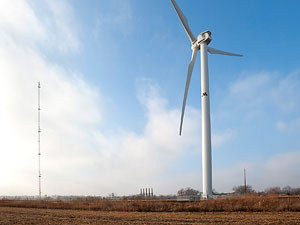
\includegraphics[width=0.5\linewidth]{wt2.jpg}		
	\caption{UMN's research turbine \cite{eolos}.
	}
	\label{fig:wt}
\end{figure}

\subsection*{Nonlinear Model} An industrial high-fidelity nonlinear simulation model
of the Clipper wind turbine in the Fatigue, Aerodynamics, Structures, and Turbulence (FAST)
simulator \cite{Fastv7_05} is used. The overall model features a detailed structural
model with various degrees of freedom of the turbine and simulates steady aerodynamics. Linear
first order models for actuators and sensors are included. The generator
dynamics are neglected, as the power electronics on modern utility-scale wind
turbines ensure a much faster torque response time than encountered in the rest
of the system.
The model is augmented with the certified  Clipper baseline control law for the different
wind regimes as described above. This baseline law includes protection functions
that reduce the torque and power overshoots in region 3 in case of turbulence.

\subsection*{Linear Parameter-Varying Model} The FAST code provides algorithms to trim the model around a defined operating point and to derive linearized models for different rotary positions \cite{Fastv7_05}. In this way, a periodic state space model in
a gridded format is available.
% EDIT BY JULIAN
The model is of 17$^{\text{th}}$ order and includes the rotary shaft velocity,
four states to describe the tower fore-aft and side-to-side flexibility, as well
as six  states to describe the first flapwise bending and six states to describe
the first edgewise bending of the blades in the rotary frame.

The MBC transformation cannot only be applied to signals but also allows the conversion of a periodic state space model from a rotating into a non-rotating coordinate system.
The derivation of the state transformation is not provided here [SHOULD WE ADDIT?] due to a lack of space, but interested readers find clear derivations in \cite{Bir08,Seiler_13}.
As for the signals, the flapwise and edgewise states are transformed to symmetric
and asymmetric states, also referred to as collective and cyclic states \cite{bir97}. 
While the MBC transformation still results in a periodic system,
analyses have shown that this transformed system can be approximated well by an
LTI model obtained from averaging over the rotary position \cite{Bir08}.
Such a model serves as the design model for the individual blade-pitch
controller in this paper.
Its inputs are the cyclic pitch commands $\beta_\text{cos}$ and
$\beta_\text{sin}$ as defined in \eqref{eq:mbc_input} and its outputs are
the cyclic moments $M_\text{cos}$ and $M_\text{sin}$ as defined in
\eqref{eq:mbc_output}.
It can be shown that cyclic pitch commands do not influence the collective
load of the turbine. 
This is an important fact, as the individual blade-pitch control algorithm should not change the thrust and the torque of the turbine in order to maintain the power output at its desired level.

% Julian starting 14.07.2016 vvvvvvvvvvvvvvvvvvvvvvvvvvvvvvvvvvvvvvvvvvvvvvvvvvvvvvvvvvvvvvvvvvvvvvvvv
Having dealt with the periodicity of the system by applying the MBC transformation, it remains to address the variation of the dynamics for different wind speeds.
The framework of linear parameter-varying (LPV) systems is a natural choice in this case. 
LPV systems are dynamic systems whose state space representations depend continuously on a time-varying external scheduling parameter $\rho\of{t}$:
\begin{equation}\label{eq:lpv_parametric}
G_\rho\colon
\begin{cases}
\dot{x}\!\left(t\right) =
A\!\left(\rho\of{t}\right)\,x\!\left(t\right) +
B\!\left(\rho\of{t}\right)\,u\!\left(t\right)
			  \\
z\!\left(t\right) =
C\!\left(\rho\of{t}\right)\,x\!\left(t\right) +
D\!\left(\rho\of{t}\right)\,y\!\left(t\right)\;.
\end{cases}
\end{equation} 
The parameter  $\rho\colon \mathds{R}\!\mapsto\!\mathcal{P}$ is confined to a compact set $\mathcal{P}\subset\mathds{R}$ of allowable parameter values. 
Additionally, the parameter rates $\dot{\rho}\colon
\mathds{R} \!\mapsto\! \mathcal{V}$ are restricted to a polyhedron
$\mathcal{V}= \left\{\dot{\rho}\in\mathds{R} \mid |\dot{\rho}| \leq \nu\right\}$ and hence the set of all admissible parameter trajectories is $\mathcal{A} = \left\{\rho(t) \mid \rho\of{t}\in\mathcal{P} \wedge \dot{\rho}\of{t}\in\mathcal{V} \quad \forall t\in\mathds{R}\right\}$.

% The continuous matrix functions $A\colon\mathcal{P}\!\mapsto\!\mathds{R}^{n_x\times n_x}$, $B\colon\mathcal{P}\!\mapsto\!\mathds{R}^{n_x\times n_w}$, $C\colon\mathcal{P}\!\mapsto\!\mathds{R}^{n_z\times n_x}$, $D\colon\mathcal{P}\!\mapsto\!\mathds{R}^{n_z\times n_w}$, the state $x\colon \mathds{R}\!\mapsto\!\mathds{R}^{n_x}$, input $u\colon \mathds{R}\!\mapsto\!\mathds{R}^{n_w}$, and output $y\colon \mathds{R}\!\mapsto\!\mathds{R}^{n_z}$ constitute a state space model


Such a model can be obtained by applying the previously described procedure (linearization, MBC-transformation, and averaging) for different wind speeds along the baseline controller scheduling trajectory, defined by generator torque and blade pitch angle.
Doing so yields a set of LTI models that together form a grid representation of the LPV system with the wind speed as its scheduling parameter. 
Linear interpolation is then used to recover models that are between two grid points.
Such a representation is not only efficient in terms of computational storage requirements but also immediately relates to intuition about linear systems since, evaluated pointwise in the parameter domain, the model recovers the LTI system that would have been obtained from linearization at that particular wind speed.   
For the Clipper model, four different fixed wind speeds of 12\,m/s, 16\,m/s, 20\,m/s, and 25\,m/s are selected to form the LPV model.
These wind speeds cover the whole region 3 range of operation.
The rate bounds, i.\,e., the maximum variation of the wind speed, are selected as $\pm$1\,m/s$^2$. COMMENT ON THESE CHOICES?


\begin{figure}[b]
	\centering
	% This file was created by matlab2tikz.
%
%The latest updates can be retrieved from
%  http://www.mathworks.com/matlabcentral/fileexchange/22022-matlab2tikz-matlab2tikz
%where you can also make suggestions and rate matlab2tikz.
%
\definecolor{mycolor1}{rgb}{0.47060,0.00000,0.52160}%
\definecolor{mycolor2}{rgb}{0.48266,0.00207,0.55504}%
\definecolor{mycolor3}{rgb}{0.49323,0.00782,0.58792}%
\definecolor{mycolor4}{rgb}{0.50197,0.01661,0.62024}%
\definecolor{mycolor5}{rgb}{0.50852,0.02778,0.65198}%
\definecolor{mycolor6}{rgb}{0.51254,0.04066,0.68311}%
\definecolor{mycolor7}{rgb}{0.51369,0.05473,0.71365}%
\definecolor{mycolor8}{rgb}{0.51270,0.07764,0.74429}%
\definecolor{mycolor9}{rgb}{0.51036,0.11095,0.77496}%
\definecolor{mycolor10}{rgb}{0.50694,0.15011,0.80497}%
\definecolor{mycolor11}{rgb}{0.50269,0.19063,0.83364}%
\definecolor{mycolor12}{rgb}{0.49790,0.22796,0.86027}%
\definecolor{mycolor13}{rgb}{0.49269,0.25790,0.88442}%
\definecolor{mycolor14}{rgb}{0.48477,0.28332,0.90982}%
\definecolor{mycolor15}{rgb}{0.47409,0.30678,0.93583}%
\definecolor{mycolor16}{rgb}{0.46173,0.32897,0.95971}%
\definecolor{mycolor17}{rgb}{0.44879,0.35061,0.97873}%
\definecolor{mycolor18}{rgb}{0.43636,0.37238,0.99014}%
\definecolor{mycolor19}{rgb}{0.42538,0.39494,0.99189}%
\definecolor{mycolor20}{rgb}{0.41513,0.41813,0.98864}%
\definecolor{mycolor21}{rgb}{0.40512,0.44146,0.98249}%
\definecolor{mycolor22}{rgb}{0.39512,0.46449,0.97420}%
\definecolor{mycolor23}{rgb}{0.38492,0.48677,0.96454}%
\definecolor{mycolor24}{rgb}{0.37428,0.50788,0.95428}%
\definecolor{mycolor25}{rgb}{0.36300,0.52746,0.94359}%
\definecolor{mycolor26}{rgb}{0.35112,0.54587,0.93005}%
\definecolor{mycolor27}{rgb}{0.33879,0.56342,0.91397}%
\definecolor{mycolor28}{rgb}{0.32615,0.58037,0.89608}%
\definecolor{mycolor29}{rgb}{0.31335,0.59699,0.87713}%
\definecolor{mycolor30}{rgb}{0.30055,0.61355,0.85786}%
\definecolor{mycolor31}{rgb}{0.28691,0.63030,0.83851}%
\definecolor{mycolor32}{rgb}{0.27045,0.64722,0.81790}%
\definecolor{mycolor33}{rgb}{0.25321,0.66401,0.79619}%
\definecolor{mycolor34}{rgb}{0.23752,0.68038,0.77365}%
\definecolor{mycolor35}{rgb}{0.22570,0.69602,0.75056}%
\definecolor{mycolor36}{rgb}{0.22008,0.71063,0.72718}%
\definecolor{mycolor37}{rgb}{0.22143,0.72415,0.70347}%
\definecolor{mycolor38}{rgb}{0.22695,0.73700,0.67896}%
\definecolor{mycolor39}{rgb}{0.23526,0.74925,0.65386}%
\definecolor{mycolor40}{rgb}{0.24504,0.76094,0.62840}%
\definecolor{mycolor41}{rgb}{0.25498,0.77214,0.60280}%
\definecolor{mycolor42}{rgb}{0.26379,0.78290,0.57729}%
\definecolor{mycolor43}{rgb}{0.27136,0.79315,0.55170}%
\definecolor{mycolor44}{rgb}{0.27885,0.80285,0.52575}%
\definecolor{mycolor45}{rgb}{0.28636,0.81217,0.49968}%
\definecolor{mycolor46}{rgb}{0.29398,0.82126,0.47373}%
\definecolor{mycolor47}{rgb}{0.30181,0.83029,0.44814}%
\definecolor{mycolor48}{rgb}{0.30995,0.83942,0.42314}%
\definecolor{mycolor49}{rgb}{0.31779,0.84897,0.39508}%
\definecolor{mycolor50}{rgb}{0.32530,0.85882,0.36382}%
\definecolor{mycolor51}{rgb}{0.33312,0.86857,0.33334}%
\definecolor{mycolor52}{rgb}{0.34191,0.87778,0.30759}%
\definecolor{mycolor53}{rgb}{0.35234,0.88605,0.29053}%
\definecolor{mycolor54}{rgb}{0.36518,0.89299,0.28587}%
\definecolor{mycolor55}{rgb}{0.38436,0.89950,0.28795}%
\definecolor{mycolor56}{rgb}{0.40984,0.90581,0.29231}%
\definecolor{mycolor57}{rgb}{0.43932,0.91154,0.29809}%
\definecolor{mycolor58}{rgb}{0.47050,0.91629,0.30439}%
\definecolor{mycolor59}{rgb}{0.50108,0.91969,0.31035}%
\definecolor{mycolor60}{rgb}{0.52910,0.92144,0.31521}%
\definecolor{mycolor61}{rgb}{0.55712,0.92265,0.31982}%
\definecolor{mycolor62}{rgb}{0.58565,0.92369,0.32445}%
\definecolor{mycolor63}{rgb}{0.61397,0.92453,0.32894}%
\definecolor{mycolor64}{rgb}{0.64138,0.92513,0.33312}%
\definecolor{mycolor65}{rgb}{0.66716,0.92545,0.33685}%
\definecolor{mycolor66}{rgb}{0.69088,0.92550,0.34002}%
\definecolor{mycolor67}{rgb}{0.71387,0.92550,0.34291}%
\definecolor{mycolor68}{rgb}{0.73606,0.92550,0.34558}%
\definecolor{mycolor69}{rgb}{0.75705,0.92550,0.34802}%
\definecolor{mycolor70}{rgb}{0.77641,0.92550,0.35023}%
\definecolor{mycolor71}{rgb}{0.79373,0.92550,0.35219}%
\definecolor{mycolor72}{rgb}{0.80868,0.92424,0.35390}%
\definecolor{mycolor73}{rgb}{0.82164,0.91723,0.35539}%
\definecolor{mycolor74}{rgb}{0.83328,0.90554,0.35672}%
\definecolor{mycolor75}{rgb}{0.84431,0.89081,0.35796}%
\definecolor{mycolor76}{rgb}{0.85539,0.87470,0.35918}%
\definecolor{mycolor77}{rgb}{0.86723,0.85886,0.36045}%
\definecolor{mycolor78}{rgb}{0.88076,0.84382,0.36189}%
\definecolor{mycolor79}{rgb}{0.89629,0.82749,0.36359}%
\definecolor{mycolor80}{rgb}{0.91245,0.80981,0.36534}%
\definecolor{mycolor81}{rgb}{0.92782,0.79087,0.36692}%
\definecolor{mycolor82}{rgb}{0.94097,0.77075,0.36808}%
\definecolor{mycolor83}{rgb}{0.95048,0.74951,0.36859}%
\definecolor{mycolor84}{rgb}{0.95699,0.72689,0.36831}%
\definecolor{mycolor85}{rgb}{0.96307,0.70242,0.36728}%
\definecolor{mycolor86}{rgb}{0.96842,0.67623,0.36557}%
\definecolor{mycolor87}{rgb}{0.97267,0.64846,0.36323}%
\definecolor{mycolor88}{rgb}{0.97548,0.61923,0.36032}%
\definecolor{mycolor89}{rgb}{0.97650,0.58870,0.35690}%
%
\definecolor{mycolor255}{rgb}{0.63529,0.07843,0.18431}%

\begin{tikzpicture}[>=stealth]
\begin{axis}[%
width=2.4in,
height=2.8in,
at={(2.722in,0.574in)},
scale only axis,
point meta min=0,
point meta max=1,
unbounded coords=jump,
xmin=-6,
xmax=1.75,
xlabel={Real part},
ymin=-0.2,
ymax=9,
hide axis,
ylabel={Imaginary part},
ylabel style = {yshift=-5mm},
axis background/.style={fill=white},
colormap={mymap}{[1pt] rgb(0pt)=(0.4706,0,0.5216); rgb(1pt)=(0.482657,0.0020652,0.555037); rgb(2pt)=(0.49323,0.00782189,0.587922); rgb(3pt)=(0.501968,0.0166117,0.620241); rgb(4pt)=(0.508522,0.0277762,0.651976); rgb(5pt)=(0.51254,0.0406571,0.683112); rgb(6pt)=(0.513685,0.054728,0.713646); rgb(7pt)=(0.5127,0.0776448,0.744287); rgb(8pt)=(0.510361,0.110947,0.774959); rgb(9pt)=(0.506936,0.150115,0.804974); rgb(10pt)=(0.502694,0.190626,0.83364); rgb(11pt)=(0.497905,0.227959,0.860268); rgb(12pt)=(0.492694,0.257901,0.884421); rgb(13pt)=(0.484773,0.283324,0.909821); rgb(14pt)=(0.474087,0.306781,0.935831); rgb(15pt)=(0.461727,0.328974,0.959713); rgb(16pt)=(0.448787,0.350605,0.978729); rgb(17pt)=(0.436358,0.372377,0.990141); rgb(18pt)=(0.425382,0.394939,0.991889); rgb(19pt)=(0.41513,0.41813,0.988645); rgb(20pt)=(0.405119,0.441458,0.982491); rgb(21pt)=(0.395123,0.464486,0.974198); rgb(22pt)=(0.384917,0.486772,0.964537); rgb(23pt)=(0.374277,0.507878,0.954276); rgb(24pt)=(0.363,0.527461,0.943585); rgb(25pt)=(0.351119,0.545869,0.930054); rgb(26pt)=(0.338786,0.563417,0.913969); rgb(27pt)=(0.326148,0.580369,0.896078); rgb(28pt)=(0.313352,0.596991,0.877126); rgb(29pt)=(0.300546,0.613549,0.857862); rgb(30pt)=(0.286908,0.6303,0.838509); rgb(31pt)=(0.27045,0.64722,0.817901); rgb(32pt)=(0.253212,0.664015,0.796189); rgb(33pt)=(0.237521,0.680382,0.773649); rgb(34pt)=(0.2257,0.696021,0.750556); rgb(35pt)=(0.220077,0.710629,0.727184); rgb(36pt)=(0.221433,0.724154,0.703468); rgb(37pt)=(0.226954,0.737003,0.678959); rgb(38pt)=(0.235259,0.749246,0.653861); rgb(39pt)=(0.245039,0.760938,0.628399); rgb(40pt)=(0.254984,0.772137,0.602801); rgb(41pt)=(0.263786,0.782897,0.577292); rgb(42pt)=(0.271359,0.79315,0.551701); rgb(43pt)=(0.278849,0.802855,0.52575); rgb(44pt)=(0.286357,0.812172,0.499679); rgb(45pt)=(0.29398,0.821264,0.47373); rgb(46pt)=(0.301814,0.830291,0.448142); rgb(47pt)=(0.309951,0.839416,0.42314); rgb(48pt)=(0.317794,0.848966,0.395079); rgb(49pt)=(0.325297,0.858822,0.363825); rgb(50pt)=(0.333118,0.868567,0.33334); rgb(51pt)=(0.341914,0.877782,0.307586); rgb(52pt)=(0.352341,0.886049,0.290526); rgb(53pt)=(0.365179,0.892991,0.285866); rgb(54pt)=(0.384362,0.899497,0.287949); rgb(55pt)=(0.409842,0.905809,0.292315); rgb(56pt)=(0.43932,0.911537,0.298088); rgb(57pt)=(0.470498,0.916292,0.304393); rgb(58pt)=(0.501079,0.919686,0.310352); rgb(59pt)=(0.529102,0.921436,0.315207); rgb(60pt)=(0.557119,0.92265,0.31982); rgb(61pt)=(0.585647,0.923695,0.324449); rgb(62pt)=(0.613973,0.924534,0.328936); rgb(63pt)=(0.641383,0.925132,0.333124); rgb(64pt)=(0.667163,0.925454,0.336853); rgb(65pt)=(0.690882,0.9255,0.340022); rgb(66pt)=(0.713869,0.9255,0.342912); rgb(67pt)=(0.736062,0.9255,0.345581); rgb(68pt)=(0.757047,0.9255,0.348021); rgb(69pt)=(0.776409,0.9255,0.350225); rgb(70pt)=(0.793734,0.9255,0.352186); rgb(71pt)=(0.808684,0.924238,0.353896); rgb(72pt)=(0.821637,0.917234,0.355386); rgb(73pt)=(0.833283,0.905539,0.35672); rgb(74pt)=(0.844307,0.890809,0.357964); rgb(75pt)=(0.855394,0.874699,0.359184); rgb(76pt)=(0.86723,0.858865,0.360447); rgb(77pt)=(0.88076,0.843823,0.361886); rgb(78pt)=(0.896288,0.82749,0.363592); rgb(79pt)=(0.912449,0.809815,0.365345); rgb(80pt)=(0.927818,0.790874,0.366916); rgb(81pt)=(0.940971,0.770746,0.368076); rgb(82pt)=(0.950483,0.749511,0.368592); rgb(83pt)=(0.956991,0.726892,0.368308); rgb(84pt)=(0.963072,0.702423,0.367281); rgb(85pt)=(0.968416,0.676232,0.365568); rgb(86pt)=(0.972672,0.648456,0.363229); rgb(87pt)=(0.975484,0.619233,0.36032); rgb(88pt)=(0.9765,0.5887,0.3569)},
colorbar,
colorbar style={ytick={0,0.09090909,0.22727, 0.31818,0.409090, 0.545454,0.77272,1} , yticklabels={3,5,8 ,10,12,15,20,25},ylabel={Wind speed},ylabel style={yshift=-25mm}}
]
\draw[-stealth,thick] (axis cs:-6,0) -- (axis cs:0.5,0) node[pos=1,right] {Re(s)};
\draw[-stealth,thick] (axis cs:0,0) -- (axis cs:0,9);%  node[pos=1,above] {Im(s)};
\addplot [color=white!15!black,dotted,forget plot]
  table[row sep=crcr]{%
0	0\\
-0	10\\
nan	nan\\
0	0\\
-1.5	9.88685996664259\\
nan	nan\\
0	0\\
-3	9.53939201416946\\
nan	nan\\
0	0\\
-4.5	8.93028554974588\\
nan	nan\\
0	0\\
-6	8\\
nan	nan\\
0	0\\
-7.5	6.61437827766148\\
nan	nan\\
0	0\\
-9	4.35889894354068\\
nan	nan\\
0	0\\
-10	0\\
nan	nan\\
0	-0\\
-0	-10\\
nan	nan\\
0	-0\\
-1.5	-9.88685996664259\\
nan	nan\\
0	-0\\
-3	-9.53939201416946\\
nan	nan\\
0	-0\\
-4.5	-8.93028554974588\\
nan	nan\\
0	-0\\
-6	-8\\
nan	nan\\
0	-0\\
-7.5	-6.61437827766148\\
nan	nan\\
0	-0\\
-9	-4.35889894354068\\
nan	nan\\
0	-0\\
-10	-0\\
nan	nan\\
};
\addplot [color=mycolor255,dashed,line width=2,forget plot]
  table[row sep=crcr]{%
-0	1.62\\
-0.04948243561574	1.61924411024575\\
-0.0989788888793362	1.61697346284848\\
-0.148502924400392	1.61317912255414\\
-0.198067193126743	1.60784619507181\\
-0.247682956575856	1.60095382601181\\
-0.297359588422165	1.59247520394303\\
-0.347104046058101	1.58237757226589\\
-0.396920304950803	1.57062225615129\\
-0.446808748952159	1.55716471250148\\
-0.496765510244563	1.54195461276636\\
-0.546781753391178	1.52493597051105\\
-0.596842899096275	1.50604732787464\\
-0.646927784873774	1.48522201746349\\
-0.697007761991798	1.46238851873337\\
-0.747045730942573	1.43747093044711\\
-0.79699512142291	1.41038958321028\\
-0.846798827541919	1.38106181819411\\
-0.896388114823515	1.34940295968371\\
-0.945681522627747	1.31532750969501\\
-0.994583793894171	1.27875059214965\\
-1.04298487352311	1.2395896714647\\
-1.09075902701397	1.19776656531543\\
-1.13776414172599	1.15320976314048\\
-1.18384128361202	1.1058570500819\\
-1.22881459149752	1.05565842000279\\
-1.27249159761694	1.0025792407557\\
-1.31466406556707	0.946603610127628\\
-1.35510943327427	0.887737812561276\\
-1.39359293714318	0.826013756268409\\
-1.42987047262014	0.761492239966402\\
-1.46369221489501	0.694265871302732\\
-1.49480698127924	0.624461438936671\\
-1.52296726520907	0.552241531489266\\
-1.54793481377775	0.477805203294009\\
-1.56948656092016	0.401387512375527\\
-1.58742067312352	0.323257801978631\\
-1.60156242102415	0.243716662465402\\
-1.61176956563061	0.16309159177256\\
-1.61793694806794	0.081731463198752\\
-1.62	0\\
nan	nan\\
-0	4.87\\
-0.14875275398065	4.8677276647511\\
-0.29754764743356	4.86090170621735\\
-0.446425457919696	4.84949526348064\\
-0.595424216374838	4.83346356172822\\
-0.744577776866927	4.81274390906018\\
-0.893914318281447	4.7872557056806\\
-1.04345475574256	4.75690047958944\\
-1.19321104019161	4.72156196756591\\
-1.34318432555371	4.68110626535938\\
-1.49336298450063	4.63538207664949\\
-1.64372045618212	4.5842210965363\\
-1.79421291271535	4.5274385720676\\
-1.94477673600943	4.4648340895353\\
-2.09532580302473	4.39619264582193\\
-2.2457485862286	4.32128606868977\\
-2.39590508724048	4.23987485816919\\
-2.54562363588219	4.15171052753416\\
-2.69469760443859	4.0565385269504\\
-2.84288210814637	3.95410183470042\\
-2.98989078781766	3.84414529862271\\
-3.13539279880097	3.72642080248957\\
-3.27901016145559	3.60069331671985\\
-3.42031566062073	3.46674786820625\\
-3.55883151308058	3.32439742833263\\
-3.69402904974871	3.17349167000839\\
-3.82532967925587	3.01392648301252\\
-3.95210740698249	2.84565406254417\\
-4.07369317286772	2.66869330072433\\
-4.18938123696746	2.48314011915256\\
-4.29843777880253	2.28917728928172\\
-4.40011178181401	2.08708320570636\\
-4.49364814742585	1.87723901705036\\
-4.5783028281285	1.66013349281032\\
-4.65335959450473	1.43636502471718\\
-4.71814787140813	1.20664023782026\\
-4.77206091241455	0.971768824466626\\
-4.81457345085654	0.732654411238586\\
-4.84525789174141	0.490281513538498\\
-4.86379810931534	0.245698904801187\\
-4.87	0\\
nan	nan\\
};
\addplot [color=white!15!black,dotted,forget plot]
  table[row sep=crcr]{%
-0	2\\
-0.061089426860987	1.99906680277252\\
-0.122196159110292	1.99626353438084\\
-0.183336943704187	1.99157916364708\\
-0.244527398921905	1.98499530255779\\
-0.305781427871428	1.97648620495285\\
-0.367110602990327	1.96601877030004\\
-0.428523513651976	1.95355255835295\\
-0.490025067840498	1.939039822409\\
-0.55161573944711	1.92242557098948\\
-0.613290753388349	1.90364767008193\\
-0.675039201717504	1.88263700063092\\
-0.736843085304044	1.85931768873413\\
-0.798676277621943	1.83360742896727\\
-0.860503409866418	1.80541792436219\\
-0.922278680176015	1.77465546968779\\
-0.983944594349272	1.74122170766702\\
-1.04543065128632	1.7050145903631\\
-1.10665199360928	1.66592957985643\\
-1.16750805262685	1.62386112308025\\
-1.22788122702984	1.57870443475265\\
-1.28763564632483	1.53035761909223\\
-1.3466160827333	1.47872415471041\\
-1.40464708855061	1.42371575696355\\
-1.46153244890373	1.36525561738506\\
-1.5170550512315	1.30328200000345\\
-1.57097728100857	1.23775214908112\\
-1.62304205625564	1.16864643225633\\
-1.67297460898058	1.09597260810034\\
-1.72048510758417	1.01977006946717\\
-1.76527218841993	0.940113876501731\\
-1.80702742579631	0.857118359633003\\
-1.84544071762869	0.770940048069964\\
-1.88020650025811	0.681779668505267\\
-1.91103063429352	0.589882967029641\\
-1.93763772953106	0.495540138735218\\
-1.95977860879447	0.399083706146458\\
-1.97723755681993	0.300884768475805\\
-1.98983896991434	0.201347644163654\\
-1.9974530223061	0.100903040986114\\
-2	0\\
nan	nan\\
-0	4\\
-0.122178853372197	3.99813360554505\\
-0.244392318220583	3.99252706876168\\
-0.366673887408374	3.98315832729416\\
-0.48905479784381	3.96999060511558\\
-0.611562855742855	3.9529724099057\\
-0.734221205980654	3.93203754060008\\
-0.857047027303953	3.9071051167059\\
-0.980050135680996	3.87807964481799\\
-1.10323147889422	3.84485114197895\\
-1.2265815067767	3.80729534016385\\
-1.35007840343501	3.76527400126184\\
-1.47368617060809	3.71863537746826\\
-1.59735255524389	3.66721485793454\\
-1.72100681973284	3.61083584872437\\
-1.84455736035203	3.54931093937558\\
-1.96788918869854	3.48244341533404\\
-2.09086130257264	3.41002918072621\\
-2.21330398721856	3.33185915971285\\
-2.3350161052537	3.24772224616051\\
-2.45576245405968	3.15740886950531\\
-2.57527129264966	3.06071523818446\\
-2.6932321654666	2.95744830942082\\
-2.80929417710122	2.8474315139271\\
-2.92306489780746	2.73051123477012\\
-3.03411010246301	2.60656400000689\\
-3.14195456201714	2.47550429816223\\
-3.24608411251129	2.33729286451266\\
-3.34594921796117	2.19194521620068\\
-3.44097021516834	2.03954013893434\\
-3.53054437683986	1.88022775300346\\
-3.61405485159262	1.71423671926601\\
-3.69088143525737	1.54188009613993\\
-3.76041300051622	1.36355933701053\\
-3.82206126858705	1.17976593405928\\
-3.87527545906212	0.991080277470437\\
-3.91955721758895	0.798167412292917\\
-3.95447511363987	0.60176953695161\\
-3.97967793982867	0.402695288327308\\
-3.99490604461219	0.201806081972227\\
-4	0\\
nan	nan\\
-0	6\\
-0.183268280058296	5.99720040831757\\
-0.366588477330875	5.98879060314253\\
-0.550010831112562	5.97473749094124\\
-0.733582196765714	5.95498590767337\\
-0.917344283614283	5.92945861485854\\
-1.10133180897098	5.89805631090012\\
-1.28557054095593	5.86065767505886\\
-1.47007520352149	5.81711946722699\\
-1.65484721834133	5.76727671296843\\
-1.83987226016505	5.71094301024578\\
-2.02511760515251	5.64791100189277\\
-2.21052925591213	5.57795306620238\\
-2.39602883286583	5.50082228690181\\
-2.58151022959925	5.41625377308656\\
-2.76683604052805	5.32396640906337\\
-2.95183378304782	5.22366512300105\\
-3.13629195385896	5.11504377108931\\
-3.31995598082783	4.99778873956928\\
-3.50252415788054	4.87158336924076\\
-3.68364368108952	4.73611330425796\\
-3.8629069389745	4.59107285727668\\
-4.0398482481999	4.43617246413123\\
-4.21394126565183	4.27114727089065\\
-4.38459734671119	4.09576685215519\\
-4.55116515369451	3.90984600001034\\
-4.71293184302571	3.71325644724335\\
-4.86912616876693	3.50593929676899\\
-5.01892382694175	3.28791782430102\\
-5.16145532275252	3.05931020840151\\
-5.29581656525979	2.82034162950519\\
-5.42108227738892	2.57135507889901\\
-5.53632215288606	2.31282014420989\\
-5.64061950077433	2.0453390055158\\
-5.73309190288057	1.76964890108892\\
-5.81291318859318	1.48662041620566\\
-5.87933582638343	1.19725111843938\\
-5.9317126704598	0.902654305427415\\
-5.96951690974301	0.604042932490963\\
-5.99235906691829	0.302709122958341\\
-6	0\\
nan	nan\\
-0	8\\
-0.244357706744395	7.9962672110901\\
-0.488784636441166	7.98505413752337\\
-0.733347774816749	7.96631665458832\\
-0.978109595687619	7.93998121023116\\
-1.22312571148571	7.90594481981139\\
-1.46844241196131	7.86407508120016\\
-1.71409405460791	7.81421023341181\\
-1.96010027136199	7.75615928963599\\
-2.20646295778844	7.68970228395791\\
-2.4531630135534	7.61459068032771\\
-2.70015680687001	7.53054800252369\\
-2.94737234121617	7.43727075493651\\
-3.19470511048777	7.33442971586908\\
-3.44201363946567	7.22167169744875\\
-3.68911472070406	7.09862187875116\\
-3.93577837739709	6.96488683066807\\
-4.18172260514528	6.82005836145241\\
-4.42660797443711	6.66371831942571\\
-4.67003221050739	6.49544449232102\\
-4.91152490811936	6.31481773901061\\
-5.15054258529933	6.12143047636891\\
-5.3864643309332	5.91489661884164\\
-5.61858835420243	5.69486302785421\\
-5.84612979561492	5.46102246954025\\
-6.06822020492601	5.21312800001378\\
-6.28390912403428	4.95100859632446\\
-6.49216822502258	4.67458572902532\\
-6.69189843592233	4.38389043240136\\
-6.88194043033669	4.07908027786869\\
-7.06108875367972	3.76045550600693\\
-7.22810970318523	3.42847343853201\\
-7.38176287051475	3.08376019227986\\
-7.52082600103244	2.72711867402107\\
-7.64412253717409	2.35953186811856\\
-7.75055091812424	1.98216055494087\\
-7.8391144351779	1.59633482458583\\
-7.90895022727974	1.20353907390322\\
-7.95935587965734	0.805390576654617\\
-7.98981208922438	0.403612163944455\\
-8	0\\
nan	nan\\
% -0	10\\
% -0.305447133430494	9.99533401386262\\
% -0.610980795551458	9.98131767190421\\
% -0.916684718520936	9.95789581823541\\
% -1.22263699460952	9.92497651278894\\
% -1.52890713935714	9.88243102476424\\
% -1.83555301495164	9.8300938515002\\
% -2.14261756825988	9.76776279176476\\
% -2.45012533920249	9.69519911204499\\
% -2.75807869723555	9.61212785494739\\
% -3.06645376694175	9.51823835040964\\
% -3.37519600858752	9.41318500315461\\
% -3.68421542652022	9.29658844367064\\
% -3.99338138810971	9.16803714483634\\
% -4.30251704933209	9.02708962181094\\
% -4.61139340088008	8.87327734843895\\
% -4.91972297174636	8.70610853833509\\
% -5.2271532564316	8.52507295181552\\
% -5.53325996804639	8.32964789928214\\
% -5.83754026313424	8.11930561540127\\
% -6.1394061351492	7.89352217376326\\
% -6.43817823162416	7.65178809546114\\
% -6.73308041366651	7.39362077355205\\
% -7.02323544275304	7.11857878481776\\
% -7.30766224451865	6.82627808692531\\
% -7.58527525615752	6.51641000001723\\
% -7.85488640504285	6.18876074540558\\
% -8.11521028127822	5.84323216128165\\
% -8.36487304490292	5.4798630405017\\
% -8.60242553792086	5.09885034733586\\
% -8.82636094209965	4.70056938250866\\
% -9.03513712898154	4.28559179816501\\
% -9.22720358814343	3.85470024034982\\
% -9.40103250129055	3.40889834252633\\
% -9.55515317146762	2.9494148351482\\
% -9.6881886476553	2.47770069367609\\
% -9.79889304397237	1.99541853073229\\
% -9.88618778409967	1.50442384237903\\
% -9.94919484957168	1.00673822081827\\
% -9.98726511153048	0.504515204930568\\
% -10	0\\
% nan	nan\\
-0	-1.62\\
-0.04948243561574	-1.61924411024575\\
-0.0989788888793362	-1.61697346284848\\
-0.148502924400392	-1.61317912255414\\
-0.198067193126743	-1.60784619507181\\
-0.247682956575856	-1.60095382601181\\
-0.297359588422165	-1.59247520394303\\
-0.347104046058101	-1.58237757226589\\
-0.396920304950803	-1.57062225615129\\
-0.446808748952159	-1.55716471250148\\
-0.496765510244563	-1.54195461276636\\
-0.546781753391178	-1.52493597051105\\
-0.596842899096275	-1.50604732787464\\
-0.646927784873774	-1.48522201746349\\
-0.697007761991798	-1.46238851873337\\
-0.747045730942573	-1.43747093044711\\
-0.79699512142291	-1.41038958321028\\
-0.846798827541919	-1.38106181819411\\
-0.896388114823515	-1.34940295968371\\
-0.945681522627747	-1.31532750969501\\
-0.994583793894171	-1.27875059214965\\
-1.04298487352311	-1.2395896714647\\
-1.09075902701397	-1.19776656531543\\
-1.13776414172599	-1.15320976314048\\
-1.18384128361202	-1.1058570500819\\
-1.22881459149752	-1.05565842000279\\
-1.27249159761694	-1.0025792407557\\
-1.31466406556707	-0.946603610127628\\
-1.35510943327427	-0.887737812561276\\
-1.39359293714318	-0.826013756268409\\
-1.42987047262014	-0.761492239966402\\
-1.46369221489501	-0.694265871302732\\
-1.49480698127924	-0.624461438936671\\
-1.52296726520907	-0.552241531489266\\
-1.54793481377775	-0.477805203294009\\
-1.56948656092016	-0.401387512375527\\
-1.58742067312352	-0.323257801978631\\
-1.60156242102415	-0.243716662465402\\
-1.61176956563061	-0.16309159177256\\
-1.61793694806794	-0.081731463198752\\
-1.62	-0\\
nan	nan\\
-0	-2\\
-0.0610894266860987	-1.99906680277252\\
-0.122196159110292	-1.99626353438084\\
-0.183336943704187	-1.99157916364708\\
-0.244527398921905	-1.98499530255779\\
-0.305781427871428	-1.97648620495285\\
-0.367110602990327	-1.96601877030004\\
-0.428523513651976	-1.95355255835295\\
-0.490025067840498	-1.939039822409\\
-0.55161573944711	-1.92242557098948\\
-0.613290753388349	-1.90364767008193\\
-0.675039201717504	-1.88263700063092\\
-0.736843085304044	-1.85931768873413\\
-0.798676277621943	-1.83360742896727\\
-0.860503409866418	-1.80541792436219\\
-0.922278680176015	-1.77465546968779\\
-0.983944594349272	-1.74122170766702\\
-1.04543065128632	-1.7050145903631\\
-1.10665199360928	-1.66592957985643\\
-1.16750805262685	-1.62386112308025\\
-1.22788122702984	-1.57870443475265\\
-1.28763564632483	-1.53035761909223\\
-1.3466160827333	-1.47872415471041\\
-1.40464708855061	-1.42371575696355\\
-1.46153244890373	-1.36525561738506\\
-1.5170550512315	-1.30328200000345\\
-1.57097728100857	-1.23775214908112\\
-1.62304205625564	-1.16864643225633\\
-1.67297460898058	-1.09597260810034\\
-1.72048510758417	-1.01977006946717\\
-1.76527218841993	-0.940113876501731\\
-1.80702742579631	-0.857118359633003\\
-1.84544071762869	-0.770940048069964\\
-1.88020650025811	-0.681779668505267\\
-1.91103063429352	-0.589882967029641\\
-1.93763772953106	-0.495540138735218\\
-1.95977860879447	-0.399083706146458\\
-1.97723755681993	-0.300884768475805\\
-1.98983896991434	-0.201347644163654\\
-1.9974530223061	-0.100903040986114\\
-2	-0\\
nan	nan\\
-0	-4\\
-0.122178853372197	-3.99813360554505\\
-0.244392318220583	-3.99252706876168\\
-0.366673887408374	-3.98315832729416\\
-0.48905479784381	-3.96999060511558\\
-0.611562855742855	-3.9529724099057\\
-0.734221205980654	-3.93203754060008\\
-0.857047027303953	-3.9071051167059\\
-0.980050135680996	-3.87807964481799\\
-1.10323147889422	-3.84485114197895\\
-1.2265815067767	-3.80729534016385\\
-1.35007840343501	-3.76527400126184\\
-1.47368617060809	-3.71863537746826\\
-1.59735255524389	-3.66721485793454\\
-1.72100681973284	-3.61083584872437\\
-1.84455736035203	-3.54931093937558\\
-1.96788918869854	-3.48244341533404\\
-2.09086130257264	-3.41002918072621\\
-2.21330398721856	-3.33185915971285\\
-2.3350161052537	-3.24772224616051\\
-2.45576245405968	-3.15740886950531\\
-2.57527129264966	-3.06071523818446\\
-2.6932321654666	-2.95744830942082\\
-2.80929417710122	-2.8474315139271\\
-2.92306489780746	-2.73051123477012\\
-3.03411010246301	-2.60656400000689\\
-3.14195456201714	-2.47550429816223\\
-3.24608411251129	-2.33729286451266\\
-3.34594921796117	-2.19194521620068\\
-3.44097021516834	-2.03954013893434\\
-3.53054437683986	-1.88022775300346\\
-3.61405485159262	-1.71423671926601\\
-3.69088143525737	-1.54188009613993\\
-3.76041300051622	-1.36355933701053\\
-3.82206126858705	-1.17976593405928\\
-3.87527545906212	-0.991080277470437\\
-3.91955721758895	-0.798167412292917\\
-3.95447511363987	-0.60176953695161\\
-3.97967793982867	-0.402695288327308\\
-3.99490604461219	-0.201806081972227\\
-4	-0\\
nan	nan\\
-0	-4.87\\
-0.14875275398065	-4.8677276647511\\
-0.29754764743356	-4.86090170621735\\
-0.446425457919696	-4.84949526348064\\
-0.595424216374838	-4.83346356172822\\
-0.744577776866927	-4.81274390906018\\
-0.893914318281447	-4.7872557056806\\
-1.04345475574256	-4.75690047958944\\
-1.19321104019161	-4.72156196756591\\
-1.34318432555371	-4.68110626535938\\
-1.49336298450063	-4.63538207664949\\
-1.64372045618212	-4.5842210965363\\
-1.79421291271535	-4.5274385720676\\
-1.94477673600943	-4.4648340895353\\
-2.09532580302473	-4.39619264582193\\
-2.2457485862286	-4.32128606868977\\
-2.39590508724048	-4.23987485816919\\
-2.54562363588219	-4.15171052753416\\
-2.69469760443859	-4.0565385269504\\
-2.84288210814637	-3.95410183470042\\
-2.98989078781766	-3.84414529862271\\
-3.13539279880097	-3.72642080248957\\
-3.27901016145559	-3.60069331671985\\
-3.42031566062073	-3.46674786820625\\
-3.55883151308058	-3.32439742833263\\
-3.69402904974871	-3.17349167000839\\
-3.82532967925587	-3.01392648301252\\
-3.95210740698249	-2.84565406254417\\
-4.07369317286772	-2.66869330072433\\
-4.18938123696746	-2.48314011915256\\
-4.29843777880253	-2.28917728928172\\
-4.40011178181401	-2.08708320570636\\
-4.49364814742585	-1.87723901705036\\
-4.5783028281285	-1.66013349281032\\
-4.65335959450473	-1.43636502471718\\
-4.71814787140813	-1.20664023782026\\
-4.77206091241455	-0.971768824466626\\
-4.81457345085654	-0.732654411238586\\
-4.84525789174141	-0.490281513538498\\
-4.86379810931534	-0.245698904801187\\
-4.87	-0\\
nan	nan\\
-0	-6\\
-0.183268280058296	-5.99720040831757\\
-0.366588477330875	-5.98879060314253\\
-0.550010831112562	-5.97473749094124\\
-0.733582196765714	-5.95498590767337\\
-0.917344283614283	-5.92945861485854\\
-1.10133180897098	-5.89805631090012\\
-1.28557054095593	-5.86065767505886\\
-1.47007520352149	-5.81711946722699\\
-1.65484721834133	-5.76727671296843\\
-1.83987226016505	-5.71094301024578\\
-2.02511760515251	-5.64791100189277\\
-2.21052925591213	-5.57795306620238\\
-2.39602883286583	-5.50082228690181\\
-2.58151022959925	-5.41625377308656\\
-2.76683604052805	-5.32396640906337\\
-2.95183378304782	-5.22366512300105\\
-3.13629195385896	-5.11504377108931\\
-3.31995598082783	-4.99778873956928\\
-3.50252415788054	-4.87158336924076\\
-3.68364368108952	-4.73611330425796\\
-3.8629069389745	-4.59107285727668\\
-4.0398482481999	-4.43617246413123\\
-4.21394126565183	-4.27114727089065\\
-4.38459734671119	-4.09576685215519\\
-4.55116515369451	-3.90984600001034\\
-4.71293184302571	-3.71325644724335\\
-4.86912616876693	-3.50593929676899\\
-5.01892382694175	-3.28791782430102\\
-5.16145532275252	-3.05931020840151\\
-5.29581656525979	-2.82034162950519\\
-5.42108227738892	-2.57135507889901\\
-5.53632215288606	-2.31282014420989\\
-5.64061950077433	-2.0453390055158\\
-5.73309190288057	-1.76964890108892\\
-5.81291318859318	-1.48662041620566\\
-5.87933582638343	-1.19725111843938\\
-5.9317126704598	-0.902654305427415\\
-5.96951690974301	-0.604042932490963\\
-5.99235906691829	-0.302709122958341\\
-6	-0\\
nan	nan\\
-0	-8\\
-0.244357706744395	-7.9962672110901\\
-0.488784636441166	-7.98505413752337\\
-0.733347774816749	-7.96631665458832\\
-0.978109595687619	-7.93998121023116\\
-1.22312571148571	-7.90594481981139\\
-1.46844241196131	-7.86407508120016\\
-1.71409405460791	-7.81421023341181\\
-1.96010027136199	-7.75615928963599\\
-2.20646295778844	-7.68970228395791\\
-2.4531630135534	-7.61459068032771\\
-2.70015680687001	-7.53054800252369\\
-2.94737234121617	-7.43727075493651\\
-3.19470511048777	-7.33442971586908\\
-3.44201363946567	-7.22167169744875\\
-3.68911472070406	-7.09862187875116\\
-3.93577837739709	-6.96488683066807\\
-4.18172260514528	-6.82005836145241\\
-4.42660797443711	-6.66371831942571\\
-4.67003221050739	-6.49544449232102\\
-4.91152490811936	-6.31481773901061\\
-5.15054258529933	-6.12143047636891\\
-5.3864643309332	-5.91489661884164\\
-5.61858835420243	-5.69486302785421\\
-5.84612979561492	-5.46102246954025\\
-6.06822020492601	-5.21312800001378\\
-6.28390912403428	-4.95100859632446\\
-6.49216822502258	-4.67458572902532\\
-6.69189843592233	-4.38389043240136\\
-6.88194043033669	-4.07908027786869\\
-7.06108875367972	-3.76045550600693\\
-7.22810970318523	-3.42847343853201\\
-7.38176287051475	-3.08376019227986\\
-7.52082600103244	-2.72711867402107\\
-7.64412253717409	-2.35953186811856\\
-7.75055091812424	-1.98216055494087\\
-7.8391144351779	-1.59633482458583\\
-7.90895022727974	-1.20353907390322\\
-7.95935587965734	-0.805390576654617\\
-7.98981208922438	-0.403612163944455\\
-8	-0\\
nan	nan\\
-0	-10\\
-0.305447133430494	-9.99533401386262\\
-0.610980795551458	-9.98131767190421\\
-0.916684718520936	-9.95789581823541\\
-1.22263699460952	-9.92497651278894\\
-1.52890713935714	-9.88243102476424\\
-1.83555301495164	-9.8300938515002\\
-2.14261756825988	-9.76776279176476\\
-2.45012533920249	-9.69519911204499\\
-2.75807869723555	-9.61212785494739\\
-3.06645376694175	-9.51823835040964\\
-3.37519600858752	-9.41318500315461\\
-3.68421542652022	-9.29658844367064\\
-3.99338138810971	-9.16803714483634\\
-4.30251704933209	-9.02708962181094\\
-4.61139340088008	-8.87327734843895\\
-4.91972297174636	-8.70610853833509\\
-5.2271532564316	-8.52507295181552\\
-5.53325996804639	-8.32964789928214\\
-5.83754026313424	-8.11930561540127\\
-6.1394061351492	-7.89352217376326\\
-6.43817823162416	-7.65178809546114\\
-6.73308041366651	-7.39362077355205\\
-7.02323544275304	-7.11857878481776\\
-7.30766224451865	-6.82627808692531\\
-7.58527525615752	-6.51641000001723\\
-7.85488640504285	-6.18876074540558\\
-8.11521028127822	-5.84323216128165\\
-8.36487304490292	-5.4798630405017\\
-8.60242553792086	-5.09885034733586\\
-8.82636094209965	-4.70056938250866\\
-9.03513712898154	-4.28559179816501\\
-9.22720358814343	-3.85470024034982\\
-9.40103250129055	-3.40889834252633\\
-9.55515317146762	-2.9494148351482\\
-9.6881886476553	-2.47770069367609\\
-9.79889304397237	-1.99541853073229\\
-9.88618778409967	-1.50442384237903\\
-9.94919484957168	-1.00673822081827\\
-9.98726511153048	-0.504515204930568\\
-10	-0\\
nan	nan\\
};
\node[above left, align=right, text=black](fw) at (axis cs:-2.5,4.5) {flapwise};
\draw [->,thick,dashed] (fw) -- +(1cm,0.7cm);
\draw [->,thick,dashed] (fw) -- +(1.2cm,-0.3cm);
\draw [->,thick,dashed] (fw) -- +(1.5cm,-1.5cm);
\node[above left, align=right, text=black](ew) at (axis cs:-0.5,7) {edgewise};
\draw [->,thick,dashed] (ew) -- +(1cm,0.7cm);
\draw [->,thick,dashed] (ew) -- +(1cm,-1.3cm);
\node[above left, align=right, text=black]
at (axis cs:-0.3,1.8) {Tower};
\node[above left, align=right, text=black!70!darkgray]
at (axis cs:0.5,7.8) {8};
\node[above left, align=right, text=black!70!darkgray]
at (axis cs:0.5,5.8) {6};
%\node[above left, align=right, text=black!70!darkgray]
%at (axis cs:0.8,4.6) {\color{mycolor255}3P};
\node[above left, align=right, text=black!70!darkgray]
at (axis cs:0.5,3.8) {4};
\node[above left, align=right, text=black!70!darkgray]
at (axis cs:0.5,1.8) {2};
%\node[above left, align=right, text=black!70!darkgray]
%at (axis cs:0.8,1.3) {\color{mycolor255}1P};
\node[right, align=left, text=black!70!darkgray]
at (axis cs:-5.895,2.855) {0.9};
\node[right, align=left, text=black!70!darkgray]
at (axis cs:-5.895,5.199) {0.75};
\node[right, align=left, text=black!70!darkgray]
at (axis cs:-5.895,7.86) {0.6};
\node[below, align=center, text=black!70!darkgray]
at (axis cs:-4.467,8.865) {0.45};
\node[below, align=center, text=black!70!darkgray]
at (axis cs:-2.788,8.865) {0.3};
\node[below, align=center, text=black!70!darkgray]
at (axis cs:-1.345,8.865) {0.15};
\addplot [color=mycolor1,line width=2.0pt,only marks,mark=x,mark options={solid},forget plot]
  table[row sep=crcr]{%
-0.154712246305915	13.7622272936341\\
-0.154712246305915	-13.7622272936341\\
-0.0438959629188374	7.04409777384228\\
-0.0438959629188374	-7.04409777384228\\
-0.0437228469922087	5.91205196945775\\
-0.0437228469922087	-5.91205196945775\\
-0.387223482887234	4.65950618433553\\
-0.387223482887234	-4.65950618433553\\
-0.374413331572446	4.25882381087047\\
-0.374413331572446	-4.25882381087047\\
-0.389527059491948	3.56800990672485\\
-0.389527059491948	-3.56800990672485\\
-0.016451012413991	0\\
-0.044120963377418	2.01682005673859\\
-0.044120963377418	-2.01682005673859\\
-0.00479228767815224	2.06064218844052\\
-0.00479228767815224	-2.06064218844052\\
};
\addplot [color=mycolor2,line width=2.0pt,only marks,mark=x,mark options={solid},forget plot]
  table[row sep=crcr]{%
-0.155280438833858	13.7665762479038\\
-0.155280438833858	-13.7665762479038\\
-0.0448262821597899	7.0908253340686\\
-0.0448262821597899	-7.0908253340686\\
-0.0447590780435397	5.87074390576286\\
-0.0447590780435397	-5.87074390576286\\
-0.418474112812987	4.71000848400016\\
-0.418474112812987	-4.71000848400016\\
-0.404103526449164	4.2670605442425\\
-0.404103526449164	-4.2670605442425\\
-0.420499561311128	3.53327250552832\\
-0.420499561311128	-3.53327250552832\\
-0.0164047599292314	0\\
-0.0475255047611054	2.0171984399919\\
-0.0475255047611054	-2.0171984399919\\
-0.00484641187463569	2.06065640819418\\
-0.00484641187463569	-2.06065640819418\\
};
\addplot [color=mycolor3,line width=2.0pt,only marks,mark=x,mark options={solid},forget plot]
  table[row sep=crcr]{%
-0.155826157783428	13.7714566634048\\
-0.155826157783428	-13.7714566634048\\
-0.0457906760755632	7.13897826050697\\
-0.0457906760755632	-7.13897826050697\\
-0.0457958918321627	5.82815052815046\\
-0.0457958918321627	-5.82815052815046\\
-0.449700098140598	4.76286710080323\\
-0.449700098140598	-4.76286710080323\\
-0.433695996602434	4.27610801813429\\
-0.433695996602434	-4.27610801813429\\
-0.451152334655131	3.49811863824046\\
-0.451152334655131	-3.49811863824046\\
-0.018220764876044	0\\
-0.0509327517895918	2.01760966083884\\
-0.0509327517895918	-2.01760966083884\\
-0.00489924621042076	2.06056906140604\\
-0.00489924621042076	-2.06056906140604\\
};
\addplot [color=mycolor4,line width=2.0pt,only marks,mark=x,mark options={solid},forget plot]
  table[row sep=crcr]{%
-0.156379304287977	13.7766243310078\\
-0.156379304287977	-13.7766243310078\\
-0.0468098302084554	7.18809613634306\\
-0.0468098302084554	-7.18809613634306\\
-0.0468121918496511	5.78516439750053\\
-0.0468121918496511	-5.78516439750053\\
-0.480871463270557	4.81722754495269\\
-0.480871463270557	-4.81722754495269\\
-0.463256769936809	4.28588270297865\\
-0.463256769936809	-4.28588270297865\\
-0.481594888898501	3.46311134005467\\
-0.481594888898501	-3.46311134005467\\
-0.0190936641888319	0\\
-0.0543322532420995	2.01804988779144\\
-0.0543322532420995	-2.01804988779144\\
-0.00495071008369105	2.06057640770434\\
-0.00495071008369105	-2.06057640770434\\
};
\addplot [color=mycolor5,line width=2.0pt,only marks,mark=x,mark options={solid},forget plot]
  table[row sep=crcr]{%
-0.156904220256201	13.7820436035224\\
-0.156904220256201	-13.7820436035224\\
-0.0477844851957774	7.23722364519961\\
-0.0477844851957774	-7.23722364519961\\
-0.0479141594674528	5.74238144142388\\
-0.0479141594674528	-5.74238144142388\\
-0.511962589806497	4.87213047952932\\
-0.511962589806497	-4.87213047952932\\
-0.49282379550999	4.29627805434425\\
-0.49282379550999	-4.29627805434425\\
-0.51194702145082	3.42888956589532\\
-0.51194702145082	-3.42888956589532\\
-0.0206734008730819	0\\
-0.0577478348745956	2.01854022209058\\
-0.0577478348745956	-2.01854022209058\\
-0.00500357503856951	2.06058526812638\\
-0.00500357503856951	-2.06058526812638\\
};
\addplot [color=mycolor6,line width=2.0pt,only marks,mark=x,mark options={solid},forget plot]
  table[row sep=crcr]{%
-0.157411370032497	13.7877063128219\\
-0.157411370032497	-13.7877063128219\\
-0.0487593244565838	7.2850672679136\\
-0.0487593244565838	-7.2850672679136\\
-0.0489497438370599	5.70125302565816\\
-0.0489497438370599	-5.70125302565816\\
-0.54317915605397	4.92580295290565\\
-0.54317915605397	-4.92580295290565\\
-0.522570263431789	4.30684263054503\\
-0.522570263431789	-4.30684263054503\\
-0.542404570104962	3.39623243903793\\
-0.542404570104962	-3.39623243903793\\
-0.0223046047562015	0\\
-0.0612064794281122	2.01910284844158\\
-0.0612064794281122	-2.01910284844158\\
-0.00505790422194391	2.0605929899453\\
-0.00505790422194391	-2.0605929899453\\
};
\addplot [color=mycolor7,line width=2.0pt,only marks,mark=x,mark options={solid},forget plot]
  table[row sep=crcr]{%
-0.157961374639601	13.7936949457083\\
-0.157961374639601	-13.7936949457083\\
-0.04981784376811	7.33453827790033\\
-0.04981784376811	-7.33453827790033\\
-0.0499992954482352	5.6587314672776\\
-0.0499992954482352	-5.6587314672776\\
-0.57425175357681	4.9819561605446\\
-0.57425175357681	-4.9819561605446\\
-0.552230335733044	4.31829983098877\\
-0.552230335733044	-4.31829983098877\\
-0.572637125114115	3.36306901020402\\
-0.572637125114115	-3.36306901020402\\
-0.0239247109057884	0\\
-0.0646163276148908	2.01970401860758\\
-0.0646163276148908	-2.01970401860758\\
-0.00511297393934584	2.0605772346535\\
-0.00511297393934584	-2.0605772346535\\
};
\addplot [color=mycolor8,line width=2.0pt,only marks,mark=x,mark options={solid},forget plot]
  table[row sep=crcr]{%
-0.158461285061409	13.79985076449\\
-0.158461285061409	-13.79985076449\\
-0.0509945080249097	7.38386544687343\\
-0.0509945080249097	-7.38386544687343\\
-0.0509062768346031	5.61657197834763\\
-0.0509062768346031	-5.61657197834763\\
-0.605408530885247	5.03849594121966\\
-0.605408530885247	-5.03849594121966\\
-0.582028785496292	4.33034543842887\\
-0.582028785496292	-4.33034543842887\\
-0.602907977113721	3.3307730341399\\
-0.602907977113721	-3.3307730341399\\
-0.0247804731353889	0\\
-0.068040500707914	2.02036839374719\\
-0.068040500707914	-2.02036839374719\\
-0.00516945838734692	2.06055478722506\\
-0.00516945838734692	-2.06055478722506\\
};
\addplot [color=mycolor9,line width=2.0pt,only marks,mark=x,mark options={solid},forget plot]
  table[row sep=crcr]{%
-0.159032164165247	13.8063253882323\\
-0.159032164165247	-13.8063253882323\\
-0.0518143728619225	7.43290585687\\
-0.0518143728619225	-7.43290585687\\
-0.0521881729029626	5.57488019020872\\
-0.0521881729029626	-5.57488019020872\\
-0.636604279964021	5.09512745632792\\
-0.636604279964021	-5.09512745632792\\
-0.611882414088297	4.34279445605007\\
-0.611882414088297	-4.34279445605007\\
-0.63315806992805	3.29924457877405\\
-0.63315806992805	-3.29924457877405\\
-0.0258781508589315	0\\
-0.0714755009940067	2.02109742827748\\
-0.0714755009940067	-2.02109742827748\\
-0.00522927825003289	2.06056281437172\\
-0.00522927825003289	-2.06056281437172\\
};
\addplot [color=mycolor10,line width=2.0pt,only marks,mark=x,mark options={solid},forget plot]
  table[row sep=crcr]{%
-0.159545716959614	13.8129051630497\\
-0.159545716959614	-13.8129051630497\\
-0.0529557004312915	7.48194124952699\\
-0.0529557004312915	-7.48194124952699\\
-0.0531292728509947	5.53353283571958\\
-0.0531292728509947	-5.53353283571958\\
-0.667873497822663	5.15208839376705\\
-0.667873497822663	-5.15208839376705\\
-0.64188212990153	4.35571565445306\\
-0.64188212990153	-4.35571565445306\\
-0.663474610687495	3.26837170115566\\
-0.663474610687495	-3.26837170115566\\
-0.0260629579848613	0\\
-0.0749018556252652	2.02188551270378\\
-0.0749018556252652	-2.02188551270378\\
-0.00529156622914805	2.06056681305969\\
-0.00529156622914805	-2.06056681305969\\
};
\addplot [color=mycolor11,line width=2.0pt,only marks,mark=x,mark options={solid},forget plot]
  table[row sep=crcr]{%
-0.160043915548316	13.8198152008057\\
-0.160043915548316	-13.8198152008057\\
-0.053991601225602	7.53110795496534\\
-0.053991601225602	-7.53110795496534\\
-0.0541421114412955	5.4926519176958\\
-0.0541421114412955	-5.4926519176958\\
-0.699112326547211	5.20938673619329\\
-0.699112326547211	-5.20938673619329\\
-0.671897402940556	4.36907097875296\\
-0.671897402940556	-4.36907097875296\\
-0.693703803558668	3.23810567004593\\
-0.693703803558668	-3.23810567004593\\
-0.0282796965377254	0\\
-0.0783184188281565	2.02275724300831\\
-0.0783184188281565	-2.02275724300831\\
-0.00535722073088098	2.06047350646586\\
-0.00535722073088098	-2.06047350646586\\
};
\addplot [color=mycolor12,line width=2.0pt,only marks,mark=x,mark options={solid},forget plot]
  table[row sep=crcr]{%
-0.16056371080196	13.827177127688\\
-0.16056371080196	-13.827177127688\\
-0.0550534890332408	7.58159608027172\\
-0.0550534890332408	-7.58159608027172\\
-0.055159440856495	5.45018254221538\\
-0.055159440856495	-5.45018254221538\\
-0.730313844498723	5.26925105104375\\
-0.730313844498723	-5.26925105104375\\
-0.70193426552803	4.38348436949049\\
-0.70193426552803	-4.38348436949049\\
-0.723865210065502	3.20753978239453\\
-0.723865210065502	-3.20753978239453\\
-0.0299017760529342	0\\
-0.0817033849220976	2.02365817451588\\
-0.0817033849220976	-2.02365817451588\\
-0.00542471406985043	2.06042688949057\\
-0.00542471406985043	-2.06042688949057\\
};
\addplot [color=mycolor13,line width=2.0pt,only marks,mark=x,mark options={solid},forget plot]
  table[row sep=crcr]{%
-0.161072837688797	13.8344725234754\\
-0.161072837688797	-13.8344725234754\\
-0.0560596437794947	7.63139335760134\\
-0.0560596437794947	-7.63139335760134\\
-0.0562229578015037	5.40896927148196\\
-0.0562229578015037	-5.40896927148196\\
-0.761643739173524	5.32850555287814\\
-0.761643739173524	-5.32850555287814\\
-0.732107973465308	4.39818373183066\\
-0.732107973465308	-4.39818373183066\\
-0.754145096539149	3.17817492022518\\
-0.754145096539149	-3.17817492022518\\
-0.0308021306485453	0\\
-0.0850589552660919	2.02454597562656\\
-0.0850589552660919	-2.02454597562656\\
-0.00549756304944946	2.06038005785601\\
-0.00549756304944946	-2.06038005785601\\
};
\addplot [color=mycolor14,line width=2.0pt,only marks,mark=x,mark options={solid},forget plot]
  table[row sep=crcr]{%
-0.161660401557013	13.8420312924953\\
-0.161660401557013	-13.8420312924953\\
-0.0571008197909133	7.68140367297893\\
-0.0571008197909133	-7.68140367297893\\
-0.793104552487753	5.38845984030101\\
-0.793104552487753	-5.38845984030101\\
-0.0572382233969586	5.36754247082125\\
-0.0572382233969586	-5.36754247082125\\
-0.762464117553079	4.41328130894367\\
-0.762464117553079	-4.41328130894367\\
-0.784524373920924	3.14896390161895\\
-0.784524373920924	-3.14896390161895\\
-0.0324147191693518	0\\
-0.0884074665310025	2.02555500877994\\
-0.0884074665310025	-2.02555500877994\\
-0.0055739768384192	2.06038366709986\\
-0.0055739768384192	-2.06038366709986\\
};
\addplot [color=mycolor15,line width=2.0pt,only marks,mark=x,mark options={solid},forget plot]
  table[row sep=crcr]{%
-0.162161604835191	13.8497724021774\\
-0.162161604835191	-13.8497724021774\\
-0.0580696276312438	7.73072167323568\\
-0.0580696276312438	-7.73072167323568\\
-0.824652040440053	5.4480440308384\\
-0.824652040440053	-5.4480440308384\\
-0.0583099724364561	5.32699740055625\\
-0.0583099724364561	-5.32699740055625\\
-0.792931808752519	4.42878296443255\\
-0.792931808752519	-4.42878296443255\\
-0.815001982969404	3.12096820607576\\
-0.815001982969404	-3.12096820607576\\
-0.0333973400631744	0\\
-0.0917223989421884	2.02666155115588\\
-0.0917223989421884	-2.02666155115588\\
-0.00565555674738305	2.06035943067577\\
-0.00565555674738305	-2.06035943067577\\
};
\addplot [color=mycolor16,line width=2.0pt,only marks,mark=x,mark options={solid},forget plot]
  table[row sep=crcr]{%
-0.162671837333321	13.8575730630312\\
-0.162671837333321	-13.8575730630312\\
-0.0590569478635556	7.7801273380201\\
-0.0590569478635556	-7.7801273380201\\
-0.856562340097998	5.50784304287007\\
-0.856562340097998	-5.50784304287007\\
-0.0593033122196758	5.28674826536649\\
-0.0593033122196758	-5.28674826536649\\
-0.823755880657313	4.44451067491549\\
-0.823755880657313	-4.44451067491549\\
-0.845790498154068	3.09324741313686\\
-0.845790498154068	-3.09324741313686\\
-0.0350815797275403	0\\
-0.0950161824311179	2.02790255219609\\
-0.0950161824311179	-2.02790255219609\\
-0.00574055854231603	2.06033606144157\\
-0.00574055854231603	-2.06033606144157\\
};
\addplot [color=mycolor17,line width=2.0pt,only marks,mark=x,mark options={solid},forget plot]
  table[row sep=crcr]{%
-0.163170809676709	13.865852607059\\
-0.163170809676709	-13.865852607059\\
-0.0600294358700166	7.83068332869574\\
-0.0600294358700166	-7.83068332869574\\
-0.88834266404924	5.56974428381967\\
-0.88834266404924	-5.56974428381967\\
-0.0602851640417839	5.24559302970272\\
-0.0602851640417839	-5.24559302970272\\
-0.854524391215121	4.46127294972511\\
-0.854524391215121	-4.46127294972511\\
-0.876511204310938	3.06559359186559\\
-0.876511204310938	-3.06559359186559\\
-0.0362154759724785	0\\
-0.0982287620785278	2.02920692076492\\
-0.0982287620785278	-2.02920692076492\\
-0.00583062900881487	2.06034274156449\\
-0.00583062900881487	-2.06034274156449\\
};
\addplot [color=mycolor18,line width=2.0pt,only marks,mark=x,mark options={solid},forget plot]
  table[row sep=crcr]{%
-0.163702153782818	13.8741447034122\\
-0.163702153782818	-13.8741447034122\\
-0.061007786841111	7.88132238514499\\
-0.061007786841111	-7.88132238514499\\
-0.920105566803018	5.63189570701448\\
-0.920105566803018	-5.63189570701448\\
-0.0611965020177339	5.20452950843691\\
-0.0611965020177339	-5.20452950843691\\
-0.885293305839506	4.47821286323417\\
-0.885293305839506	-4.47821286323417\\
-0.907201771093297	3.03807561760203\\
-0.907201771093297	-3.03807561760203\\
-0.0378097450901487	0\\
-0.101414307798591	2.0305876994292\\
-0.101414307798591	-2.0305876994292\\
-0.0059246306902383	2.06027223319385\\
-0.0059246306902383	-2.06027223319385\\
};
\addplot [color=mycolor19,line width=2.0pt,only marks,mark=x,mark options={solid},forget plot]
  table[row sep=crcr]{%
-0.164156853049474	13.882686338667\\
-0.164156853049474	-13.882686338667\\
-0.0619754838166688	7.93209062142045\\
-0.0619754838166688	-7.93209062142045\\
-0.951688416900678	5.69475173357694\\
-0.951688416900678	-5.69475173357694\\
-0.0620782854109721	5.16356075997789\\
-0.0620782854109721	-5.16356075997789\\
-0.915880055476048	4.49580330225101\\
-0.915880055476048	-4.49580330225101\\
-0.937720751500736	3.01115533421441\\
-0.937720751500736	-3.01115533421441\\
-0.0382466149878063	0\\
-0.104514933577154	2.03203596158459\\
-0.104514933577154	-2.03203596158459\\
-0.00602440133941484	2.0602294286481\\
-0.00602440133941484	-2.0602294286481\\
};
\addplot [color=mycolor20,line width=2.0pt,only marks,mark=x,mark options={solid},forget plot]
  table[row sep=crcr]{%
-0.164627554968569	13.891457949286\\
-0.164627554968569	-13.891457949286\\
-0.0628114483769273	7.98278521233124\\
-0.0628114483769273	-7.98278521233124\\
-0.98355156516208	5.75822107097786\\
-0.98355156516208	-5.75822107097786\\
-0.063000558017115	5.1225417645194\\
-0.063000558017115	-5.1225417645194\\
-0.94677380460236	4.51393590268776\\
-0.94677380460236	-4.51393590268776\\
-0.968535075316458	2.98479691115067\\
-0.968535075316458	-2.98479691115067\\
-0.0395225981972304	0\\
-0.10755808360763	2.03340016090517\\
-0.10755808360763	-2.03340016090517\\
-0.00612907478026797	2.06015690118248\\
-0.00612907478026797	-2.06015690118248\\
};
\addplot [color=mycolor21,line width=2.0pt,only marks,mark=x,mark options={solid},forget plot]
  table[row sep=crcr]{%
-0.165161312799999	13.9004391988473\\
-0.165161312799999	-13.9004391988473\\
-0.0636896048337677	8.03388568512231\\
-0.0636896048337677	-8.03388568512231\\
-1.01539962184788	5.82239869716835\\
-1.01539962184788	-5.82239869716835\\
-0.06385472406257	5.08188906651454\\
-0.06385472406257	-5.08188906651454\\
-0.97771788655602	4.53271919114631\\
-0.97771788655602	-4.53271919114631\\
-0.999463848459354	2.95905946730128\\
-0.999463848459354	-2.95905946730128\\
-0.0413532969664867	0\\
-0.110499408586898	2.03488342383643\\
-0.110499408586898	-2.03488342383643\\
-0.00623650534651965	2.06016362116543\\
-0.00623650534651965	-2.06016362116543\\
};
\addplot [color=mycolor22,line width=2.0pt,only marks,mark=x,mark options={solid},forget plot]
  table[row sep=crcr]{%
-0.165650948266583	13.9094464360995\\
-0.165650948266583	-13.9094464360995\\
-0.0645052254097619	8.08444995462868\\
-0.0645052254097619	-8.08444995462868\\
-1.04741492200922	5.88611711107373\\
-1.04741492200922	-5.88611711107373\\
-0.0646924093008034	5.04170790894228\\
-0.0646924093008034	-5.04170790894228\\
-1.00880504028299	4.55149153753576\\
-1.00880504028299	-4.55149153753576\\
-1.03052477629244	2.93374342949407\\
-1.03052477629244	-2.93374342949407\\
-0.0425516359256487	0\\
-0.113387064972512	2.03651723746982\\
-0.113387064972512	-2.03651723746982\\
-0.00635151754492563	2.06012345121812\\
-0.00635151754492563	-2.06012345121812\\
};
\addplot [color=mycolor23,line width=2.0pt,only marks,mark=x,mark options={solid},forget plot]
  table[row sep=crcr]{%
-0.166101061388718	13.9185861141975\\
-0.166101061388718	-13.9185861141975\\
-0.0653072982658229	8.13508481273769\\
-0.0653072982658229	-8.13508481273769\\
-1.07930013318654	5.95034977101675\\
-1.07930013318654	-5.95034977101675\\
-0.0653941970074512	5.00160141584649\\
-0.0653941970074512	-5.00160141584649\\
-1.03977704384721	4.57075950573069\\
-1.03977704384721	-4.57075950573069\\
-1.06155315151128	2.90891269755844\\
-1.06155315151128	-2.90891269755844\\
-0.0434041240370733	0\\
-0.116192825725858	2.038186117292\\
-0.116192825725858	-2.038186117292\\
-0.0064679529203176	2.06013571103035\\
-0.0064679529203176	-2.06013571103035\\
};
\addplot [color=mycolor24,line width=2.0pt,only marks,mark=x,mark options={solid},forget plot]
  table[row sep=crcr]{%
-0.166583260824078	13.9279563386885\\
-0.166583260824078	-13.9279563386885\\
-0.0661586970925117	8.18637001221348\\
-0.0661586970925117	-8.18637001221348\\
-1.11152001413091	6.01547614776275\\
-1.11152001413091	-6.01547614776275\\
-0.0661828248542837	4.96114424637319\\
-0.0661828248542837	-4.96114424637319\\
-1.07111273725262	4.59035668563512\\
-1.07111273725262	-4.59035668563512\\
-1.09293941816	2.88388560133172\\
-1.09293941816	-2.88388560133172\\
-0.0453711612661877	0\\
-0.11890975380193	2.03991580978892\\
-0.11890975380193	-2.03991580978892\\
-0.00659129522801438	2.06012846419282\\
-0.00659129522801438	-2.06012846419282\\
};
\addplot [color=mycolor25,line width=2.0pt,only marks,mark=x,mark options={solid},forget plot]
  table[row sep=crcr]{%
-0.164791974887407	13.9371035095939\\
-0.164791974887407	-13.9371035095939\\
-0.0633464700402924	8.23559676125922\\
-0.0633464700402924	-8.23559676125922\\
-1.219912790529	6.06097927385316\\
-1.219912790529	-6.06097927385316\\
-1.174627856273	4.59070793538029\\
-1.174627856273	-4.59070793538029\\
-0.0636024088967206	4.92372609431485\\
-0.0636024088967206	-4.92372609431485\\
-1.19562478980387	2.8381526349659\\
-1.19562478980387	-2.8381526349659\\
-0.0401438418653742	0\\
-0.129845583599757	2.04656651200584\\
-0.129845583599757	-2.04656651200584\\
-0.00647145366637791	2.0600848536282\\
-0.00647145366637791	-2.0600848536282\\
};
\addplot [color=mycolor26,line width=2.0pt,only marks,mark=x,mark options={solid},forget plot]
  table[row sep=crcr]{%
-0.163439857592399	13.9343242238435\\
-0.163439857592399	-13.9343242238435\\
-0.061808545230996	8.23645916894962\\
-0.061808545230996	-8.23645916894962\\
-1.30877521001311	6.03586315208784\\
-1.30877521001311	-6.03586315208784\\
-1.26093553160261	4.5650202388773\\
-1.26093553160261	-4.5650202388773\\
-0.0621731538590771	4.92490796967509\\
-0.0621731538590771	-4.92490796967509\\
-1.28345891056888	2.81041885773266\\
-1.28345891056888	-2.81041885773266\\
-0.0378810776463604	0\\
-0.137329369678281	2.05132174142529\\
-0.137329369678281	-2.05132174142529\\
-0.0064752292454105	2.06012744621487\\
-0.0064752292454105	-2.06012744621487\\
};
\addplot [color=mycolor27,line width=2.0pt,only marks,mark=x,mark options={solid},forget plot]
  table[row sep=crcr]{%
-0.163348765944169	13.9320327798786\\
-0.163348765944169	-13.9320327798786\\
-0.0620238271120439	8.23682391930093\\
-0.0620238271120439	-8.23682391930093\\
-1.34554622664618	6.02390605591933\\
-1.34554622664618	-6.02390605591933\\
-1.29713852836998	4.55367168654388\\
-1.29713852836998	-4.55367168654388\\
-0.0624659119411859	4.92614556857993\\
-0.0624659119411859	-4.92614556857993\\
-1.31983574779032	2.79814589662828\\
-1.31983574779032	-2.79814589662828\\
-0.0372247367030272	0\\
-0.140126118336561	2.05347390973159\\
-0.140126118336561	-2.05347390973159\\
-0.00658563877385948	2.06015268531964\\
-0.00658563877385948	-2.06015268531964\\
};
\addplot [color=mycolor28,line width=2.0pt,only marks,mark=x,mark options={solid},forget plot]
  table[row sep=crcr]{%
-0.163184193159619	13.9294648352657\\
-0.163184193159619	-13.9294648352657\\
-0.0616948763569998	8.23797509402993\\
-0.0616948763569998	-8.23797509402993\\
-1.3889322185039	6.01088521248212\\
-1.3889322185039	-6.01088521248212\\
-0.0623111909108994	4.92654285780812\\
-0.0623111909108994	-4.92654285780812\\
-1.3400151055586	4.5405758942222\\
-1.3400151055586	-4.5405758942222\\
-1.36373897417729	2.78363301057162\\
-1.36373897417729	-2.78363301057162\\
-0.0364852796953682	0\\
-0.142500944222666	2.05540888287733\\
-0.142500944222666	-2.05540888287733\\
-0.00664500623507869	2.06010893054898\\
-0.00664500623507869	-2.06010893054898\\
};
\addplot [color=mycolor29,line width=2.0pt,only marks,mark=x,mark options={solid},forget plot]
  table[row sep=crcr]{%
-0.162731714723473	13.9265713934557\\
-0.162731714723473	-13.9265713934557\\
-0.061314690326163	8.23851259272897\\
-0.061314690326163	-8.23851259272897\\
-1.42866953430994	5.99825770193126\\
-1.42866953430994	-5.99825770193126\\
-0.0618296503937452	4.92734307063137\\
-0.0618296503937452	-4.92734307063137\\
-1.37899556097952	4.52828360559648\\
-1.37899556097952	-4.52828360559648\\
-1.40353832568927	2.77026391014479\\
-1.40353832568927	-2.77026391014479\\
-0.0364433148140151	0\\
-0.145140117032713	2.05741495611683\\
-0.145140117032713	-2.05741495611683\\
-0.0066871262694711	2.06014466428308\\
-0.0066871262694711	-2.06014466428308\\
};
\addplot [color=mycolor30,line width=2.0pt,only marks,mark=x,mark options={solid},forget plot]
  table[row sep=crcr]{%
-0.162405426964375	13.9233720414845\\
-0.162405426964375	-13.9233720414845\\
-0.060767112253981	8.23884132656072\\
-0.060767112253981	-8.23884132656072\\
-1.46282476484069	5.98698679154626\\
-1.46282476484069	-5.98698679154626\\
-0.061576488776669	4.92793078667253\\
-0.061576488776669	-4.92793078667253\\
-1.41241081834701	4.51738635373628\\
-1.41241081834701	-4.51738635373628\\
-1.43767994273457	2.75827204208325\\
-1.43767994273457	-2.75827204208325\\
-0.0360755105382659	0\\
-0.147487512225133	2.05917108879026\\
-0.147487512225133	-2.05917108879026\\
-0.00673367644903083	2.06017692336639\\
-0.00673367644903083	-2.06017692336639\\
};
\addplot [color=mycolor31,line width=2.0pt,only marks,mark=x,mark options={solid},forget plot]
  table[row sep=crcr]{%
-0.161881333773535	13.9198626838888\\
-0.161881333773535	-13.9198626838888\\
-0.0604442277404436	8.23924408140024\\
-0.0604442277404436	-8.23924408140024\\
-1.4936165092987	5.97690300824842\\
-1.4936165092987	-5.97690300824842\\
-0.0610926596114813	4.92837662610069\\
-0.0610926596114813	-4.92837662610069\\
-1.44225686461894	4.50763014144575\\
-1.44225686461894	-4.50763014144575\\
-1.46845599139019	2.7473627427016\\
-1.46845599139019	-2.7473627427016\\
-0.0359265549706454	0\\
-0.149724269381495	2.06081764108062\\
-0.149724269381495	-2.06081764108062\\
-0.00676760755002001	2.06020606647957\\
-0.00676760755002001	-2.06020606647957\\
};
\addplot [color=mycolor32,line width=2.0pt,only marks,mark=x,mark options={solid},forget plot]
  table[row sep=crcr]{%
-0.161356105011544	13.9159264511959\\
-0.161356105011544	-13.9159264511959\\
-0.0598959912461826	8.23895668745907\\
-0.0598959912461826	-8.23895668745907\\
-1.52033967764944	5.96724652635691\\
-1.52033967764944	-5.96724652635691\\
-0.0607720588287287	4.92937727554084\\
-0.0607720588287287	-4.92937727554084\\
-1.46813525668341	4.49895562620006\\
-1.46813525668341	-4.49895562620006\\
-1.4948960253958	2.7380837653788\\
-1.4948960253958	-2.7380837653788\\
-0.0357167869662377	0\\
-0.151644542774977	2.06224329128603\\
-0.151644542774977	-2.06224329128603\\
-0.00677646087070705	2.06023349499412\\
-0.00677646087070705	-2.06023349499412\\
};
\addplot [color=mycolor33,line width=2.0pt,only marks,mark=x,mark options={solid},forget plot]
  table[row sep=crcr]{%
-0.160766846008118	13.9123389988971\\
-0.160766846008118	-13.9123389988971\\
-0.0596486393490196	8.24006032296899\\
-0.0596486393490196	-8.24006032296899\\
-1.54424852822473	5.96013012035535\\
-1.54424852822473	-5.96013012035535\\
-0.060561978396604	4.92910107619142\\
-0.060561978396604	-4.92910107619142\\
-1.49142288399391	4.49157948709449\\
-1.49142288399391	-4.49157948709449\\
-1.51874174421813	2.72896639688744\\
-1.51874174421813	-2.72896639688744\\
-0.0358871646306831	0\\
-0.153204412744471	2.06351606956638\\
-0.153204412744471	-2.06351606956638\\
-0.00675182324844181	2.0602567840234\\
-0.00675182324844181	-2.0602567840234\\
};
\addplot [color=mycolor34,line width=2.0pt,only marks,mark=x,mark options={solid},forget plot]
  table[row sep=crcr]{%
-0.160255747100847	13.9079379972857\\
-0.160255747100847	-13.9079379972857\\
-0.0591494076614628	8.24060688543539\\
-0.0591494076614628	-8.24060688543539\\
-1.56305447293523	5.95434318920621\\
-1.56305447293523	-5.95434318920621\\
-0.060262071764734	4.92932648083199\\
-0.060262071764734	-4.92932648083199\\
-1.50959550603516	4.48609529673674\\
-1.50959550603516	-4.48609529673674\\
-1.53722272442094	2.7219776522304\\
-1.53722272442094	-2.7219776522304\\
-0.0361286975706955	0\\
-0.154458400623348	2.06465269812888\\
-0.154458400623348	-2.06465269812888\\
-0.00670889129012112	2.06029592139254\\
-0.00670889129012112	-2.06029592139254\\
};
\addplot [color=mycolor35,line width=2.0pt,only marks,mark=x,mark options={solid},forget plot]
  table[row sep=crcr]{%
-0.157893562022406	13.9026042677643\\
-0.157893562022406	-13.9026042677643\\
-0.0586983321372778	8.23996326107354\\
-0.0586983321372778	-8.23996326107354\\
-1.58570278585571	5.94551630264795\\
-1.58570278585571	-5.94551630264795\\
-0.059663744390355	4.93018029712485\\
-0.059663744390355	-4.93018029712485\\
-1.53120194637143	4.4783576406981\\
-1.53120194637143	-4.4783576406981\\
-1.55948088426656	2.71372210494277\\
-1.55948088426656	-2.71372210494277\\
-0.0343020606842348	0\\
-0.153983417947089	2.06635245034809\\
-0.153983417947089	-2.06635245034809\\
-0.00659752064332325	2.06029914796071\\
-0.00659752064332325	-2.06029914796071\\
};
\addplot [color=mycolor36,line width=2.0pt,only marks,mark=x,mark options={solid},forget plot]
  table[row sep=crcr]{%
-0.157384620619436	13.8926636872263\\
-0.157384620619436	-13.8926636872263\\
-0.0568237059428025	8.24016650350949\\
-0.0568237059428025	-8.24016650350949\\
-1.65138319169839	5.9238645419801\\
-1.65138319169839	-5.9238645419801\\
-0.0581647393990257	4.92913171436292\\
-0.0581647393990257	-4.92913171436292\\
-1.59283438744642	4.45576569177433\\
-1.59283438744642	-4.45576569177433\\
-1.62556553942254	2.68939161119801\\
-1.62556553942254	-2.68939161119801\\
-0.0369438103632274	0\\
-0.158445874543132	2.06908771861023\\
-0.158445874543132	-2.06908771861023\\
-0.00649620775377577	2.06030227621421\\
-0.00649620775377577	-2.06030227621421\\
};
\addplot [color=mycolor37,line width=2.0pt,only marks,mark=x,mark options={solid},forget plot]
  table[row sep=crcr]{%
-0.158045780437402	13.8790680445274\\
-0.158045780437402	-13.8790680445274\\
-0.0550789627758772	8.23942817423469\\
-0.0550789627758772	-8.23942817423469\\
-1.71752207820015	5.89910568081186\\
-1.71752207820015	-5.89910568081186\\
-0.0564202942944385	4.92882542776675\\
-0.0564202942944385	-4.92882542776675\\
-1.6533861930453	4.43155331627814\\
-1.6533861930453	-4.43155331627814\\
-1.69334869086869	2.66384715421622\\
-1.69334869086869	-2.66384715421622\\
-0.0411065401902648	0\\
-0.162715423544997	2.07018589265327\\
-0.162715423544997	-2.07018589265327\\
-0.0064416096827952	2.06029692691961\\
-0.0064416096827952	-2.06029692691961\\
};
\addplot [color=mycolor37,line width=1.0pt,only marks,mark=o,mark options={solid,mark size=3},forget plot]  %% GRID
  table[row sep=crcr]{%
-0.158045780437402	13.8790680445274\\
-0.158045780437402	-13.8790680445274\\
-0.0550789627758772	8.23942817423469\\
-0.0550789627758772	-8.23942817423469\\
-1.71752207820015	5.89910568081186\\
-1.71752207820015	-5.89910568081186\\
-0.0564202942944385	4.92882542776675\\
-0.0564202942944385	-4.92882542776675\\
-1.6533861930453	4.43155331627814\\
-1.6533861930453	-4.43155331627814\\
-1.69334869086869	2.66384715421622\\
-1.69334869086869	-2.66384715421622\\
-0.0411065401902648	0\\
-0.162715423544997	2.07018589265327\\
-0.162715423544997	-2.07018589265327\\
-0.0064416096827952	2.06029692691961\\
-0.0064416096827952	-2.06029692691961\\
};

\addplot [color=mycolor38,line width=2.0pt,only marks,mark=x,mark options={solid},forget plot]
  table[row sep=crcr]{%
-0.15869429100701	13.8642826213407\\
-0.15869429100701	-13.8642826213407\\
-0.0537110491765478	8.23787327156442\\
-0.0537110491765478	-8.23787327156442\\
-1.76031731530794	5.88118329789693\\
-1.76031731530794	-5.88118329789693\\
-0.0551268801906064	4.92954455463393\\
-0.0551268801906064	-4.92954455463393\\
-1.69164389733881	4.41598577682787\\
-1.69164389733881	-4.41598577682787\\
-1.73678351358328	2.64720509404481\\
-1.73678351358328	-2.64720509404481\\
-0.04592595772755	0\\
-0.164971642972521	2.07109045859246\\
-0.164971642972521	-2.07109045859246\\
-0.00640806885653578	2.06029945670474\\
-0.00640806885653578	-2.06029945670474\\
};
\addplot [color=mycolor39,line width=2.0pt,only marks,mark=x,mark options={solid},forget plot]
  table[row sep=crcr]{%
-0.159312768739843	13.8500631091219\\
-0.159312768739843	-13.8500631091219\\
-0.0526084111939648	8.23854674702983\\
-0.0526084111939648	-8.23854674702983\\
-1.78617265682306	5.87255191458564\\
-1.78617265682306	-5.87255191458564\\
-0.0542485414306078	4.92843907305267\\
-0.0542485414306078	-4.92843907305267\\
-1.71417875066367	4.40804542875363\\
-1.71417875066367	-4.40804542875363\\
-1.76298534300564	2.6358351516424\\
-1.76298534300564	-2.6358351516424\\
-0.0501095132209653	0\\
-0.166462242102619	2.07153622978375\\
-0.166462242102619	-2.07153622978375\\
-0.00641099402655165	2.06029998056388\\
-0.00641099402655165	-2.06029998056388\\
};
\addplot [color=mycolor40,line width=2.0pt,only marks,mark=x,mark options={solid},forget plot]
  table[row sep=crcr]{%
-0.159810687638284	13.8341331881336\\
-0.159810687638284	-13.8341331881336\\
-0.0517168082657302	8.2374407933821\\
-0.0517168082657302	-8.2374407933821\\
-1.80861468031587	5.86220356401985\\
-1.80861468031587	-5.86220356401985\\
-0.0534094320984532	4.92921371874602\\
-0.0534094320984532	-4.92921371874602\\
-1.73345387542937	4.4007426055115\\
-1.73345387542937	-4.4007426055115\\
-1.78581728977588	2.62664394935863\\
-1.78581728977588	-2.62664394935863\\
-0.0547273203006155	0\\
-0.168819344935848	2.07151214317434\\
-0.168819344935848	-2.07151214317434\\
-0.0064443834467667	2.06030118934563\\
-0.0064443834467667	-2.06030118934563\\
};
\addplot [color=mycolor41,line width=2.0pt,only marks,mark=x,mark options={solid},forget plot]
  table[row sep=crcr]{%
-0.160187933719253	13.8181134877921\\
-0.160187933719253	-13.8181134877921\\
-0.0510761488013838	8.23685481003231\\
-0.0510761488013838	-8.23685481003231\\
-1.8128793130507	5.85961063375515\\
-1.8128793130507	-5.85961063375515\\
-0.0528672851879946	4.92952433718079\\
-0.0528672851879946	-4.92952433718079\\
-1.73562548180701	4.40154948809548\\
-1.73562548180701	-4.40154948809548\\
-1.79124617610855	2.62460932053186\\
-1.79124617610855	-2.62460932053186\\
-0.0584356032698449	0\\
-0.168359203972937	2.07083494469015\\
-0.168359203972937	-2.07083494469015\\
-0.00642233047836183	2.06031804256217\\
-0.00642233047836183	-2.06031804256217\\
};
\addplot [color=mycolor42,line width=2.0pt,only marks,mark=x,mark options={solid},forget plot]
  table[row sep=crcr]{%
-0.161146028825711	13.8028882837874\\
-0.161146028825711	-13.8028882837874\\
-0.0506146024159451	8.2378852966534\\
-0.0506146024159451	-8.2378852966534\\
-1.81367725708257	5.86053321933729\\
-1.81367725708257	-5.86053321933729\\
-0.0525561467379119	4.92897910472766\\
-0.0525561467379119	-4.92897910472766\\
-1.73483916866338	4.40487302335805\\
-1.73483916866338	-4.40487302335805\\
-1.7925907845182	2.62367005191768\\
-1.7925907845182	-2.62367005191768\\
-0.0627531105574523	0\\
-0.170153095250983	2.069894456298\\
-0.170153095250983	-2.069894456298\\
-0.00653580329808773	2.06033039775837\\
-0.00653580329808773	-2.06033039775837\\
};
\addplot [color=mycolor43,line width=2.0pt,only marks,mark=x,mark options={solid},forget plot]
  table[row sep=crcr]{%
-0.163109173717455	13.7862479766576\\
-0.163109173717455	-13.7862479766576\\
-0.0501017514572184	8.2375140272156\\
-0.0501017514572184	-8.2375140272156\\
-1.83071061975185	5.85335630744262\\
-1.83071061975185	-5.85335630744262\\
-0.0522888538914073	4.92909750844871\\
-0.0522888538914073	-4.92909750844871\\
-1.74920463243152	4.40017970784158\\
-1.74920463243152	-4.40017970784158\\
-1.80812770101359	2.6156840657019\\
-1.80812770101359	-2.6156840657019\\
-0.0688009334771814	0\\
-0.172597838815506	2.07015560919971\\
-0.172597838815506	-2.07015560919971\\
-0.00662478625476726	2.06032845407069\\
-0.00662478625476726	-2.06032845407069\\
};
\addplot [color=mycolor44,line width=2.0pt,only marks,mark=x,mark options={solid},forget plot]
  table[row sep=crcr]{%
-0.163429610228476	13.7692868297685\\
-0.163429610228476	-13.7692868297685\\
-0.0498662633071933	8.23775997432296\\
-0.0498662633071933	-8.23775997432296\\
-1.84988536120649	5.84504033579871\\
-1.84988536120649	-5.84504033579871\\
-0.0518917995292685	4.92905285324458\\
-0.0518917995292685	-4.92905285324458\\
-1.76555491056567	4.39360455524496\\
-1.76555491056567	-4.39360455524496\\
-1.82634733632062	2.60610740490675\\
-1.82634733632062	-2.60610740490675\\
-0.0741104178381052	0\\
-0.17389800388246	2.07160543352928\\
-0.17389800388246	-2.07160543352928\\
-0.00661774151898645	2.06030822168509\\
-0.00661774151898645	-2.06030822168509\\
};
\addplot [color=mycolor45,line width=2.0pt,only marks,mark=x,mark options={solid},forget plot]
  table[row sep=crcr]{%
-0.164432561081647	13.752150435409\\
-0.164432561081647	-13.752150435409\\
-0.0494265203298507	8.23743513806338\\
-0.0494265203298507	-8.23743513806338\\
-1.87223649081232	5.83482857349744\\
-1.87223649081232	-5.83482857349744\\
-0.0517281360963507	4.92940456502473\\
-0.0517281360963507	-4.92940456502473\\
-1.78501289298256	4.38569839039875\\
-1.78501289298256	-4.38569839039875\\
-1.84894341120298	2.59567511098227\\
-1.84894341120298	-2.59567511098227\\
-0.0741956782223582	0\\
-0.175961197973047	2.07200061794549\\
-0.175961197973047	-2.07200061794549\\
-0.00672040021844275	2.06033581576574\\
-0.00672040021844275	-2.06033581576574\\
};
\addplot [color=mycolor46,line width=2.0pt,only marks,mark=x,mark options={solid},forget plot]
  table[row sep=crcr]{%
-0.166250768552024	13.7346298636438\\
-0.166250768552024	-13.7346298636438\\
-0.049135249065412	8.23719619309283\\
-0.049135249065412	-8.23719619309283\\
-1.90279584492278	5.82102523010295\\
-1.90279584492278	-5.82102523010295\\
-0.0514533664362893	4.92943475560813\\
-0.0514533664362893	-4.92943475560813\\
-1.81178759850214	4.37384281195277\\
-1.81178759850214	-4.37384281195277\\
-1.88026062852039	2.58114536861784\\
-1.88026062852039	-2.58114536861784\\
-0.0860111976830572	0\\
-0.177055224019709	2.0721362168888\\
-0.177055224019709	-2.0721362168888\\
-0.00683131951691296	2.06034892339894\\
-0.00683131951691296	-2.06034892339894\\
};
\addplot [color=mycolor47,line width=2.0pt,only marks,mark=x,mark options={solid},forget plot]
  table[row sep=crcr]{%
-0.167279646808176	13.717042290786\\
-0.167279646808176	-13.717042290786\\
-0.0488643445539383	8.23702470958352\\
-0.0488643445539383	-8.23702470958352\\
-1.92138607243086	5.81209170931971\\
-1.92138607243086	-5.81209170931971\\
-0.0513311053485888	4.92975080401723\\
-0.0513311053485888	-4.92975080401723\\
-1.82691038721881	4.36740107327022\\
-1.82691038721881	-4.36740107327022\\
-1.89946304234848	2.5718992727397\\
-1.89946304234848	-2.5718992727397\\
-0.0926480219386005	0\\
-0.176892688746859	2.07196396078803\\
-0.176892688746859	-2.07196396078803\\
-0.00691320975405163	2.06037534059947\\
-0.00691320975405163	-2.06037534059947\\
};
\addplot [color=mycolor48,line width=2.0pt,only marks,mark=x,mark options={solid},forget plot]
  table[row sep=crcr]{%
-0.168807482397193	13.6993056575252\\
-0.168807482397193	-13.6993056575252\\
-0.0487691119083193	8.23702757991956\\
-0.0487691119083193	-8.23702757991956\\
-1.93609838310496	5.80473369045298\\
-1.93609838310496	-5.80473369045298\\
-0.0511772059103406	4.93004289190301\\
-0.0511772059103406	-4.93004289190301\\
-1.83845555467359	4.36274699799874\\
-1.83845555467359	-4.36274699799874\\
-1.91485085293419	2.56417654541613\\
-1.91485085293419	-2.56417654541613\\
-0.0990944058271307	0\\
-0.17743940700266	2.07159736649521\\
-0.17743940700266	-2.07159736649521\\
-0.00665861530282597	2.06044547795752\\
-0.00665861530282597	-2.06044547795752\\
};
\addplot [color=mycolor49,line width=2.0pt,only marks,mark=x,mark options={solid},forget plot]
  table[row sep=crcr]{%
-0.169134553816849	13.6813924845852\\
-0.169134553816849	-13.6813924845852\\
-0.0486016659505011	8.23715089879939\\
-0.0486016659505011	-8.23715089879939\\
-1.94420679300247	5.80060346619381\\
-1.94420679300247	-5.80060346619381\\
-0.0512016522546371	4.93027190072821\\
-0.0512016522546371	-4.93027190072821\\
-1.84382787827681	4.36153506427263\\
-1.84382787827681	-4.36153506427263\\
-1.92309935205817	2.55954726794608\\
-1.92309935205817	-2.55954726794608\\
-0.104531476876359	0\\
-0.178834175972875	2.07122339671816\\
-0.178834175972875	-2.07122339671816\\
-0.00705870483410376	2.06042455646051\\
-0.00705870483410376	-2.06042455646051\\
};
\addplot [color=mycolor50,line width=2.0pt,only marks,mark=x,mark options={solid},forget plot]
  table[row sep=crcr]{%
-0.170768807341581	13.6633929700394\\
-0.170768807341581	-13.6633929700394\\
-0.0484889090605725	8.23709045683342\\
-0.0484889090605725	-8.23709045683342\\
-1.95205260852442	5.79639740422868\\
-1.95205260852442	-5.79639740422868\\
-0.0512222115907039	4.93031065855192\\
-0.0512222115907039	-4.93031065855192\\
-1.84901713439481	4.36040218943899\\
-1.84901713439481	-4.36040218943899\\
-1.93103315834351	2.55479220735875\\
-1.93103315834351	-2.55479220735875\\
-0.106441144979237	0\\
-0.180076599261774	2.07122350715301\\
-0.180076599261774	-2.07122350715301\\
-0.00723106017365105	2.0604330155398\\
-0.00723106017365105	-2.0604330155398\\
};
\addplot [color=mycolor51,line width=2.0pt,only marks,mark=x,mark options={solid},forget plot]
  table[row sep=crcr]{%
-0.171700276129568	13.6449317729165\\
-0.171700276129568	-13.6449317729165\\
-0.0484346945419043	8.23714049028375\\
-0.0484346945419043	-8.23714049028375\\
-1.95934595124081	5.79233663956491\\
-1.95934595124081	-5.79233663956491\\
-0.0512944024071689	4.93069273282519\\
-0.0512944024071689	-4.93069273282519\\
-1.85363473465552	4.35923805425289\\
-1.85363473465552	-4.35923805425289\\
-1.93832810922017	2.5503102475136\\
-1.93832810922017	-2.5503102475136\\
-0.117184577801645	0\\
-0.178793076388359	2.07091878699419\\
-0.178793076388359	-2.07091878699419\\
-0.00639394337030857	2.06043150868575\\
-0.00639394337030857	-2.06043150868575\\
};
\addplot [color=mycolor52,line width=2.0pt,only marks,mark=x,mark options={solid},forget plot]
  table[row sep=crcr]{%
-0.173453570093396	13.6264402424114\\
-0.173453570093396	-13.6264402424114\\
-0.0484797713660672	8.2372940083511\\
-0.0484797713660672	-8.2372940083511\\
-1.96549919179008	5.78871473786006\\
-1.96549919179008	-5.78871473786006\\
-0.0513377834867939	4.93114500310447\\
-0.0513377834867939	-4.93114500310447\\
-1.85723647654587	4.35882210844704\\
-1.85723647654587	-4.35882210844704\\
-1.94443298866697	2.54633525075777\\
-1.94443298866697	-2.54633525075777\\
-0.123702206771982	0\\
-0.179092662826497	2.07058765143058\\
-0.179092662826497	-2.07058765143058\\
-0.00693041868380051	2.06047037051116\\
-0.00693041868380051	-2.06047037051116\\
};
\addplot [color=mycolor53,line width=2.0pt,only marks,mark=x,mark options={solid},forget plot]
  table[row sep=crcr]{%
-0.174747628340105	13.6078059060107\\
-0.174747628340105	-13.6078059060107\\
-0.0483807882421881	8.23724659647771\\
-0.0483807882421881	-8.23724659647771\\
-1.97011793962963	5.78581200746875\\
-1.97011793962963	-5.78581200746875\\
-0.0515619434009469	4.93141220980628\\
-0.0515619434009469	-4.93141220980628\\
-1.85945806691894	4.35926547319333\\
-1.85945806691894	-4.35926547319333\\
-1.94926528210494	2.54316009324019\\
-1.94926528210494	-2.54316009324019\\
-0.130117105403806	0\\
-0.181031213835771	2.06993706593338\\
-0.181031213835771	-2.06993706593338\\
-0.00740064985726296	2.06047830993051\\
-0.00740064985726296	-2.06047830993051\\
};
\addplot [color=mycolor53,line width=1.0pt,only marks,mark=o,mark options={solid,mark size=3},forget plot] % GRID
  table[row sep=crcr]{%
-0.174747628340105	13.6078059060107\\
-0.174747628340105	-13.6078059060107\\
-0.0483807882421881	8.23724659647771\\
-0.0483807882421881	-8.23724659647771\\
-1.97011793962963	5.78581200746875\\
-1.97011793962963	-5.78581200746875\\
-0.0515619434009469	4.93141220980628\\
-0.0515619434009469	-4.93141220980628\\
-1.85945806691894	4.35926547319333\\
-1.85945806691894	-4.35926547319333\\
-1.94926528210494	2.54316009324019\\
-1.94926528210494	-2.54316009324019\\
-0.130117105403806	0\\
-0.181031213835771	2.06993706593338\\
-0.181031213835771	-2.06993706593338\\
-0.00740064985726296	2.06047830993051\\
-0.00740064985726296	-2.06047830993051\\
};

\addplot [color=mycolor54,line width=2.0pt,only marks,mark=x,mark options={solid},forget plot]
  table[row sep=crcr]{%
-0.175181792715513	13.5889930414479\\
-0.175181792715513	-13.5889930414479\\
-0.048434674176054	8.23729467952526\\
-0.048434674176054	-8.23729467952526\\
-1.97693801564616	5.78158608811255\\
-1.97693801564616	-5.78158608811255\\
-0.0516783505264802	4.93178931782682\\
-0.0516783505264802	-4.93178931782682\\
-1.86349644988044	4.35845326956885\\
-1.86349644988044	-4.35845326956885\\
-1.95616803949866	2.53861099921426\\
-1.95616803949866	-2.53861099921426\\
-0.136086108661338	0\\
-0.181452536303519	2.06960593823221\\
-0.181452536303519	-2.06960593823221\\
-0.00761745705648276	2.06045481626431\\
-0.00761745705648276	-2.06045481626431\\
};
\addplot [color=mycolor55,line width=2.0pt,only marks,mark=x,mark options={solid},forget plot]
  table[row sep=crcr]{%
-0.176260440484301	13.570000304625\\
-0.176260440484301	-13.570000304625\\
-0.0485003380158391	8.23739870974373\\
-0.0485003380158391	-8.23739870974373\\
-1.97593092042161	5.78137910175691\\
-1.97593092042161	-5.78137910175691\\
-0.0518457508068848	4.93222098599097\\
-0.0518457508068848	-4.93222098599097\\
-1.8598958231777	4.36186131987813\\
-1.8598958231777	-4.36186131987813\\
-1.95555258601118	2.53793736272733\\
-1.95555258601118	-2.53793736272733\\
-0.138420411757782	0\\
-0.181699584194317	2.06873581571194\\
-0.181699584194317	-2.06873581571194\\
-0.00778876272972756	2.06047585838458\\
-0.00778876272972756	-2.06047585838458\\
};
\addplot [color=mycolor56,line width=2.0pt,only marks,mark=x,mark options={solid},forget plot]
  table[row sep=crcr]{%
-0.178809451290122	13.5508830533658\\
-0.178809451290122	-13.5508830533658\\
-0.0486913133218798	8.23756700832812\\
-0.0486913133218798	-8.23756700832812\\
-1.97459089626387	5.78125908877113\\
-1.97459089626387	-5.78125908877113\\
-0.0519676574893881	4.93271987377865\\
-0.0519676574893881	-4.93271987377865\\
-1.85617144090261	4.36547676209417\\
-1.85617144090261	-4.36547676209417\\
-1.9545580146121	2.53747310494765\\
-1.9545580146121	-2.53747310494765\\
-0.149643874036443	0\\
-0.181223148378027	2.06788823514359\\
-0.181223148378027	-2.06788823514359\\
-0.00725128118746188	2.06044880481481\\
-0.00725128118746188	-2.06044880481481\\
};
\addplot [color=mycolor57,line width=2.0pt,only marks,mark=x,mark options={solid},forget plot]
  table[row sep=crcr]{%
-0.18029645150792	13.5315525453282\\
-0.18029645150792	-13.5315525453282\\
-0.0488070049892175	8.23778253810497\\
-0.0488070049892175	-8.23778253810497\\
-1.97055517590826	5.78212834799849\\
-1.97055517590826	-5.78212834799849\\
-0.0522083661179277	4.93308457535127\\
-0.0522083661179277	-4.93308457535127\\
-1.84973828174581	4.37015665315945\\
-1.84973828174581	-4.37015665315945\\
-1.95081469619178	2.53791537646569\\
-1.95081469619178	-2.53791537646569\\
-0.15629302974332	0\\
-0.18001200427529	2.06710732575875\\
-0.18001200427529	-2.06710732575875\\
-0.00749064810185529	2.06056284728028\\
-0.00749064810185529	-2.06056284728028\\
};
\addplot [color=mycolor58,line width=2.0pt,only marks,mark=x,mark options={solid},forget plot]
  table[row sep=crcr]{%
-0.180725113309363	13.5121374616837\\
-0.180725113309363	-13.5121374616837\\
-0.048836024715569	8.23769949451436\\
-0.048836024715569	-8.23769949451436\\
-1.97179791711786	5.78057544471747\\
-1.97179791711786	-5.78057544471747\\
-0.0525422280405057	4.93352378728658\\
-0.0525422280405057	-4.93352378728658\\
-1.84869981807383	4.37255671777731\\
-1.84869981807383	-4.37255671777731\\
-1.95196179965524	2.53629428037175\\
-1.95196179965524	-2.53629428037175\\
-0.162477368226063	0\\
-0.180550214671078	2.06640092365076\\
-0.180550214671078	-2.06640092365076\\
-0.00757627498863184	2.06057132730748\\
-0.00757627498863184	-2.06057132730748\\
};
\addplot [color=mycolor59,line width=2.0pt,only marks,mark=x,mark options={solid},forget plot]
  table[row sep=crcr]{%
-0.182207042375533	13.4925526578687\\
-0.182207042375533	-13.4925526578687\\
-0.0490634471901855	8.23789926030008\\
-0.0490634471901855	-8.23789926030008\\
-1.96817149684563	5.78131416010358\\
-1.96817149684563	-5.78131416010358\\
-0.0526594261024012	4.93407727586902\\
-0.0526594261024012	-4.93407727586902\\
-1.84275617844799	4.37730640632977\\
-1.84275617844799	-4.37730640632977\\
-1.94850396989705	2.53669685113096\\
-1.94850396989705	-2.53669685113096\\
-0.169203320367508	0\\
-0.180444568054214	2.06553051750291\\
-0.180444568054214	-2.06553051750291\\
-0.00771385548236433	2.06062554595064\\
-0.00771385548236433	-2.06062554595064\\
};
\addplot [color=mycolor60,line width=2.0pt,only marks,mark=x,mark options={solid},forget plot]
  table[row sep=crcr]{%
-0.182597618769463	13.4727901396629\\
-0.182597618769463	-13.4727901396629\\
-0.0491179260048785	8.23785226580442\\
-0.0491179260048785	-8.23785226580442\\
-1.96657568455552	5.78104390952181\\
-1.96657568455552	-5.78104390952181\\
-0.0529844911820785	4.93477876019255\\
-0.0529844911820785	-4.93477876019255\\
-1.83876146536696	4.38117871901721\\
-1.83876146536696	-4.38117871901721\\
-1.9466532284086	2.53640194333159\\
-1.9466532284086	-2.53640194333159\\
-0.17541793215376	0\\
-0.181555072645287	2.06490454785442\\
-0.181555072645287	-2.06490454785442\\
-0.00837868178997936	2.06060437367607\\
-0.00837868178997936	-2.06060437367607\\
};
\addplot [color=mycolor61,line width=2.0pt,only marks,mark=x,mark options={solid},forget plot]
  table[row sep=crcr]{%
-0.183873493479076	13.4528604174583\\
-0.183873493479076	-13.4528604174583\\
-0.0493655884571096	8.23787531478655\\
-0.0493655884571096	-8.23787531478655\\
-1.96821965743429	5.77915986308809\\
-1.96821965743429	-5.77915986308809\\
-0.053098959554218	4.93515009912177\\
-0.053098959554218	-4.93515009912177\\
-1.83800470607374	4.38314482720566\\
-1.83800470607374	-4.38314482720566\\
-1.94826391415642	2.5343802346454\\
-1.94826391415642	-2.5343802346454\\
-0.182499587090228	0\\
-0.181803836399505	2.06444650573383\\
-0.181803836399505	-2.06444650573383\\
-0.00856343762455369	2.06063728689053\\
-0.00856343762455369	-2.06063728689053\\
};
\addplot [color=mycolor62,line width=2.0pt,only marks,mark=x,mark options={solid},forget plot]
  table[row sep=crcr]{%
-0.185104916984006	13.4329281474455\\
-0.185104916984006	-13.4329281474455\\
-0.0495450405703632	8.2383367318583\\
-0.0495450405703632	-8.2383367318583\\
-1.96986771611844	5.7774830608657\\
-1.96986771611844	-5.7774830608657\\
-0.0533640371022417	4.93576704817307\\
-0.0533640371022417	-4.93576704817307\\
-1.83699767200427	4.38514969570232\\
-1.83699767200427	-4.38514969570232\\
-1.94977747669162	2.53222829372338\\
-1.94977747669162	-2.53222829372338\\
-0.18972737053539	0\\
-0.182077895190158	2.06399893664646\\
-0.182077895190158	-2.06399893664646\\
-0.00874218756194539	2.06060495298593\\
-0.00874218756194539	-2.06060495298593\\
};
\addplot [color=mycolor63,line width=2.0pt,only marks,mark=x,mark options={solid},forget plot]
  table[row sep=crcr]{%
-0.188301185602198	13.4128762088303\\
-0.188301185602198	-13.4128762088303\\
-0.0497069885590906	8.23839809312161\\
-0.0497069885590906	-8.23839809312161\\
-1.97690533731384	5.77290617474747\\
-1.97690533731384	-5.77290617474747\\
-0.0536273815355317	4.93617688454039\\
-0.0536273815355317	-4.93617688454039\\
-1.84117834658162	4.38423069965733\\
-1.84117834658162	-4.38423069965733\\
-1.95687799781952	2.5275742305089\\
-1.95687799781952	-2.5275742305089\\
-0.194816613991721	0\\
-0.181262512073112	2.06377224010674\\
-0.181262512073112	-2.06377224010674\\
-0.00833178842620003	2.06072670247696\\
-0.00833178842620003	-2.06072670247696\\
};
\addplot [color=mycolor64,line width=2.0pt,only marks,mark=x,mark options={solid},forget plot]
  table[row sep=crcr]{%
-0.19013338009301	13.3927637695257\\
-0.19013338009301	-13.3927637695257\\
-0.0499148894741949	8.23849654955471\\
-0.0499148894741949	-8.23849654955471\\
-1.98366990915947	5.76850986781862\\
-1.98366990915947	-5.76850986781862\\
-0.0538234071265475	4.93661909403283\\
-0.0538234071265475	-4.93661909403283\\
-1.84493295162025	4.3834522293431\\
-1.84493295162025	-4.3834522293431\\
-1.96375575510242	2.52313153902757\\
-1.96375575510242	-2.52313153902757\\
-0.205940644618755	0\\
-0.181037171333411	2.06372648964448\\
-0.181037171333411	-2.06372648964448\\
-0.00760960632827001	2.060628039474\\
-0.00760960632827001	-2.060628039474\\
};
\addplot [color=mycolor65,line width=2.0pt,only marks,mark=x,mark options={solid},forget plot]
  table[row sep=crcr]{%
-0.191493819137393	13.3723537673718\\
-0.191493819137393	-13.3723537673718\\
-0.0499855624134762	8.23873860611808\\
-0.0499855624134762	-8.23873860611808\\
-1.994013951024	5.7622341707976\\
-1.994013951024	-5.7622341707976\\
-0.054190458772283	4.93701949481489\\
-0.054190458772283	-4.93701949481489\\
-1.85206557882254	4.38065419717917\\
-1.85206557882254	-4.38065419717917\\
-1.97456909419887	2.51631621398254\\
-1.97456909419887	-2.51631621398254\\
-0.214422659275694	0\\
-0.181321165901282	2.06351198163894\\
-0.181321165901282	-2.06351198163894\\
-0.00773817069344696	2.0606320206841\\
-0.00773817069344696	-2.0606320206841\\
};
\addplot [color=mycolor66,line width=2.0pt,only marks,mark=x,mark options={solid},forget plot]
  table[row sep=crcr]{%
-0.192716889819838	13.3521151361911\\
-0.192716889819838	-13.3521151361911\\
-0.0503239638088493	8.23880621068956\\
-0.0503239638088493	-8.23880621068956\\
-2.00015769642346	5.75797754536499\\
-2.00015769642346	-5.75797754536499\\
-0.0543611033643541	4.93781927821089\\
-0.0543611033643541	-4.93781927821089\\
-1.85492755731122	4.38036388528079\\
-1.85492755731122	-4.38036388528079\\
-1.98073862370587	2.51208880644074\\
-1.98073862370587	-2.51208880644074\\
-0.222551129244794	0\\
-0.181945279678491	2.06295861376296\\
-0.181945279678491	-2.06295861376296\\
-0.00870256591778654	2.06073303241351\\
-0.00870256591778654	-2.06073303241351\\
};
\addplot [color=mycolor67,line width=2.0pt,only marks,mark=x,mark options={solid},forget plot]
  table[row sep=crcr]{%
-0.193306956834395	13.3316688339519\\
-0.193306956834395	-13.3316688339519\\
-0.050401426702364	8.23904810049166\\
-0.050401426702364	-8.23904810049166\\
-2.00561715056027	5.75441343504627\\
-2.00561715056027	-5.75441343504627\\
-0.0547510875279806	4.93819940149758\\
-0.0547510875279806	-4.93819940149758\\
-1.85730912859125	4.38048700056679\\
-1.85730912859125	-4.38048700056679\\
-1.98645302296858	2.5078878127489\\
-1.98645302296858	-2.5078878127489\\
-0.229930445567558	0\\
-0.183025689847833	2.0624497319278\\
-0.183025689847833	-2.0624497319278\\
-0.00874765711948705	2.06076279614362\\
-0.00874765711948705	-2.06076279614362\\
};
\addplot [color=mycolor68,line width=2.0pt,only marks,mark=x,mark options={solid},forget plot]
  table[row sep=crcr]{%
-0.194691244391357	13.3113682121915\\
-0.194691244391357	-13.3113682121915\\
-0.0506258295355533	8.23906707552705\\
-0.0506258295355533	-8.23906707552705\\
-2.00857454108899	5.75137157785128\\
-2.00857454108899	-5.75137157785128\\
-0.0550560271619527	4.93876903870819\\
-0.0550560271619527	-4.93876903870819\\
-1.85733847347334	4.38156464918319\\
-1.85733847347334	-4.38156464918319\\
-1.98964299089324	2.50493900307038\\
-1.98964299089324	-2.50493900307038\\
-0.23801301534261	0\\
-0.183107752342985	2.06195598294513\\
-0.183107752342985	-2.06195598294513\\
-0.00891104972652901	2.06076144307744\\
-0.00891104972652901	-2.06076144307744\\
};
\addplot [color=mycolor69,line width=2.0pt,only marks,mark=x,mark options={solid},forget plot]
  table[row sep=crcr]{%
-0.194549847013919	13.2909412689655\\
-0.194549847013919	-13.2909412689655\\
-0.0508691107769208	8.23930388726651\\
-0.0508691107769208	-8.23930388726651\\
-2.01565412212818	5.74686186053643\\
-2.01565412212818	-5.74686186053643\\
-0.055335573825581	4.93915154409272\\
-0.055335573825581	-4.93915154409272\\
-1.86111864495109	4.38058744989908\\
-1.86111864495109	-4.38058744989908\\
-1.99697279463573	2.49975570614248\\
-1.99697279463573	-2.49975570614248\\
-0.245177819142538	0\\
-0.183090986889902	2.061757409568\\
-0.183090986889902	-2.061757409568\\
-0.00911454806533174	2.06080835520344\\
-0.00911454806533174	-2.06080835520344\\
};
\addplot [color=mycolor69,line width=1.0pt,only marks,mark=o,mark options={solid, mark size=3},forget plot]  %GRID
  table[row sep=crcr]{%
-0.194549847013919	13.2909412689655\\
-0.194549847013919	-13.2909412689655\\
-0.0508691107769208	8.23930388726651\\
-0.0508691107769208	-8.23930388726651\\
-2.01565412212818	5.74686186053643\\
-2.01565412212818	-5.74686186053643\\
-0.055335573825581	4.93915154409272\\
-0.055335573825581	-4.93915154409272\\
-1.86111864495109	4.38058744989908\\
-1.86111864495109	-4.38058744989908\\
-1.99697279463573	2.49975570614248\\
-1.99697279463573	-2.49975570614248\\
-0.245177819142538	0\\
-0.183090986889902	2.061757409568\\
-0.183090986889902	-2.061757409568\\
-0.00911454806533174	2.06080835520344\\
-0.00911454806533174	-2.06080835520344\\
};

\addplot [color=mycolor70,line width=2.0pt,only marks,mark=x,mark options={solid},forget plot]
  table[row sep=crcr]{%
-0.195384239439968	13.2703872972881\\
-0.195384239439968	-13.2703872972881\\
-0.0511177372006748	8.23955295211387\\
-0.0511177372006748	-8.23955295211387\\
-2.02320937001047	5.74208496766089\\
-2.02320937001047	-5.74208496766089\\
-0.0556193160089904	4.9397321854188\\
-0.0556193160089904	-4.9397321854188\\
-1.86524892632666	4.37949595306934\\
-1.86524892632666	-4.37949595306934\\
-2.00460747319608	2.49449635272162\\
-2.00460747319608	-2.49449635272162\\
-0.252776166381205	0\\
-0.183278946735039	2.06143097946708\\
-0.183278946735039	-2.06143097946708\\
-0.00989261681640813	2.0608036046234\\
-0.00989261681640813	-2.0608036046234\\
};
\addplot [color=mycolor71,line width=2.0pt,only marks,mark=x,mark options={solid},forget plot]
  table[row sep=crcr]{%
-0.196040845252201	13.2498267353785\\
-0.196040845252201	-13.2498267353785\\
-0.0513645305076054	8.23971367514703\\
-0.0513645305076054	-8.23971367514703\\
-2.02797662710783	5.73861951374979\\
-2.02797662710783	-5.73861951374979\\
-0.0559439082026385	4.9402398525648\\
-0.0559439082026385	-4.9402398525648\\
-1.8668260745929	4.37997915358573\\
-1.8668260745929	-4.37997915358573\\
-2.00960352442842	2.49082100201741\\
-2.00960352442842	-2.49082100201741\\
-0.260582083121195	0\\
-0.18338339823754	2.0610157142781\\
-0.18338339823754	-2.0610157142781\\
-0.0100764423619678	2.06077867967286\\
-0.0100764423619678	-2.06077867967286\\
};
\addplot [color=mycolor72,line width=2.0pt,only marks,mark=x,mark options={solid},forget plot]
  table[row sep=crcr]{%
-0.196802977150662	13.2291365598144\\
-0.196802977150662	-13.2291365598144\\
-0.0515240116988576	8.23987598944626\\
-0.0515240116988576	-8.23987598944626\\
-2.03428875415338	5.7340325325407\\
-2.03428875415338	-5.7340325325407\\
-0.0563076966865326	4.94073446539614\\
-0.0563076966865326	-4.94073446539614\\
-1.86980252294703	4.37931429003008\\
-1.86980252294703	-4.37931429003008\\
-2.01611178331372	2.48591581759077\\
-2.01611178331372	-2.48591581759077\\
-0.268561507035998	0\\
-0.183478698592661	2.06069534237387\\
-0.183478698592661	-2.06069534237387\\
-0.0102692494769033	2.06075703419882\\
-0.0102692494769033	-2.06075703419882\\
};
\addplot [color=mycolor73,line width=2.0pt,only marks,mark=x,mark options={solid},forget plot]
  table[row sep=crcr]{%
-0.198362998341196	13.208345732198\\
-0.198362998341196	-13.208345732198\\
-0.051870872642565	8.24000210088203\\
-0.051870872642565	-8.24000210088203\\
-2.03924944629583	5.73028589650648\\
-2.03924944629583	-5.73028589650648\\
-0.0565176578600302	4.94142502328017\\
-0.0565176578600302	-4.94142502328017\\
-1.87128988730897	4.37955125419519\\
-1.87128988730897	-4.37955125419519\\
-2.0211878594043	2.48188871054613\\
-2.0211878594043	-2.48188871054613\\
-0.277343206613591	0\\
-0.183480119056651	2.06012489391655\\
-0.183480119056651	-2.06012489391655\\
-0.0105565531649559	2.06077470096405\\
-0.0105565531649559	-2.06077470096405\\
};
\addplot [color=mycolor74,line width=2.0pt,only marks,mark=x,mark options={solid},forget plot]
  table[row sep=crcr]{%
-0.198821017397915	13.18769107756\\
-0.198821017397915	-13.18769107756\\
-0.0520279812455535	8.24029680919524\\
-0.0520279812455535	-8.24029680919524\\
-2.04380765895046	5.72708562450297\\
-2.04380765895046	-5.72708562450297\\
-0.0569380337196258	4.94189193992234\\
-0.0569380337196258	-4.94189193992234\\
-1.87233974620093	4.3801650178441\\
-1.87233974620093	-4.3801650178441\\
-2.02590457183001	2.47802924139992\\
-2.02590457183001	-2.47802924139992\\
-0.285405448021394	0\\
-0.183217059907448	2.05968684637222\\
-0.183217059907448	-2.05968684637222\\
-0.0107148917678065	2.06079467695751\\
-0.0107148917678065	-2.06079467695751\\
};
\addplot [color=mycolor75,line width=2.0pt,only marks,mark=x,mark options={solid},forget plot]
  table[row sep=crcr]{%
-0.200664607055884	13.1668798711954\\
-0.200664607055884	-13.1668798711954\\
-0.0522287317624304	8.24038121238437\\
-0.0522287317624304	-8.24038121238437\\
-2.04922532253634	5.72295291204735\\
-2.04922532253634	-5.72295291204735\\
-0.0573109749666037	4.94253739691023\\
-0.0573109749666037	-4.94253739691023\\
-1.87414859002835	4.38011833732828\\
-1.87414859002835	-4.38011833732828\\
-2.03144027947477	2.47360477967433\\
-2.03144027947477	-2.47360477967433\\
-0.294382266048087	0\\
-0.182793390848127	2.05922329436387\\
-0.182793390848127	-2.05922329436387\\
-0.0091203244684197	2.06090493501558\\
-0.0091203244684197	-2.06090493501558\\
};
\addplot [color=mycolor76,line width=2.0pt,only marks,mark=x,mark options={solid},forget plot]
  table[row sep=crcr]{%
-0.203250838295826	13.1460231696433\\
-0.203250838295826	-13.1460231696433\\
-0.0525240765237691	8.24057104167587\\
-0.0525240765237691	-8.24057104167587\\
-2.05594992808911	5.71867575544235\\
-2.05594992808911	-5.71867575544235\\
-0.0574826419939644	4.94303206506441\\
-0.0574826419939644	-4.94303206506441\\
-1.87727845912144	4.379566462858\\
-1.87727845912144	-4.379566462858\\
-2.03820323591686	2.46868072879842\\
-2.03820323591686	-2.46868072879842\\
-0.302749804432551	0\\
-0.181560474485956	2.05918469477326\\
-0.181560474485956	-2.05918469477326\\
-0.00920735781774118	2.06086679961868\\
-0.00920735781774118	-2.06086679961868\\
};
\addplot [color=mycolor77,line width=2.0pt,only marks,mark=x,mark options={solid},forget plot]
  table[row sep=crcr]{%
-0.204646622100388	13.1253259102502\\
-0.204646622100388	-13.1253259102502\\
-0.0526099965908891	8.24084274545955\\
-0.0526099965908891	-8.24084274545955\\
-2.05919737814238	5.71576339752978\\
-2.05919737814238	-5.71576339752978\\
-0.0579719819748468	4.94365045138963\\
-0.0579719819748468	-4.94365045138963\\
-1.87713625352364	4.38055412358196\\
-1.87713625352364	-4.38055412358196\\
-2.04158472777553	2.46536901394969\\
-2.04158472777553	-2.46536901394969\\
-0.307814175954957	0\\
-0.179727927734218	2.05916237526726\\
-0.179727927734218	-2.05916237526726\\
-0.00942492939386436	2.06100843504618\\
-0.00942492939386436	-2.06100843504618\\
};
\addplot [color=mycolor78,line width=2.0pt,only marks,mark=x,mark options={solid},forget plot]
  table[row sep=crcr]{%
-0.207012430989422	13.1043823120538\\
-0.207012430989422	-13.1043823120538\\
-0.0530225609079991	8.24107756248881\\
-0.0530225609079991	-8.24107756248881\\
-2.06196507182939	5.71314211022602\\
-2.06196507182939	-5.71314211022602\\
-0.058093244418335	4.94419656442682\\
-0.058093244418335	-4.94419656442682\\
-1.8767389649662	4.38212456013579\\
-1.8767389649662	-4.38212456013579\\
-2.04442051644596	2.46243037913574\\
-2.04442051644596	-2.46243037913574\\
-0.319411193341984	0\\
-0.179056049630357	2.05874804053152\\
-0.179056049630357	-2.05874804053152\\
-0.00953124712653486	2.06110709123217\\
-0.00953124712653486	-2.06110709123217\\
};
\addplot [color=mycolor79,line width=2.0pt,only marks,mark=x,mark options={solid},forget plot]
  table[row sep=crcr]{%
-0.207836317888412	13.0832402332086\\
-0.207836317888412	-13.0832402332086\\
-0.0532472327177114	8.24129840700682\\
-0.0532472327177114	-8.24129840700682\\
-2.06604278264865	5.70979571325192\\
-2.06604278264865	-5.70979571325192\\
-0.0584888146147204	4.94459082018846\\
-0.0584888146147204	-4.94459082018846\\
-1.8774568608782	4.38294911370857\\
-1.8774568608782	-4.38294911370857\\
-2.04868178450365	2.45859411074766\\
-2.04868178450365	-2.45859411074766\\
-0.331003161556541	0\\
-0.179022110582118	2.05820228988553\\
-0.179022110582118	-2.05820228988553\\
-0.00975876914976354	2.06111717003562\\
-0.00975876914976354	-2.06111717003562\\
};
\addplot [color=mycolor80,line width=2.0pt,only marks,mark=x,mark options={solid},forget plot]
  table[row sep=crcr]{%
-0.209205769062354	13.0625440492207\\
-0.209205769062354	-13.0625440492207\\
-0.0535653463622587	8.24161723672353\\
-0.0535653463622587	-8.24161723672353\\
-2.06972290163907	5.70655958931227\\
-2.06972290163907	-5.70655958931227\\
-0.0587396696340839	4.94524441405554\\
-0.0587396696340839	-4.94524441405554\\
-1.87784112145122	4.3838455919113\\
-1.87784112145122	-4.3838455919113\\
-2.05254661174101	2.4550492861755\\
-2.05254661174101	-2.4550492861755\\
-0.336700249062673	0\\
-0.177911485857259	2.05802109161913\\
-0.177911485857259	-2.05802109161913\\
-0.00980972261516111	2.06107540185136\\
-0.00980972261516111	-2.06107540185136\\
};
\addplot [color=mycolor81,line width=2.0pt,only marks,mark=x,mark options={solid},forget plot]
  table[row sep=crcr]{%
-0.210877614971313	13.0415280412215\\
-0.210877614971313	-13.0415280412215\\
-0.05382938411535	8.2416824707823\\
-0.05382938411535	-8.2416824707823\\
-2.07337470343235	5.70327231233048\\
-2.07337470343235	-5.70327231233048\\
-0.0590837373148093	4.94584544981139\\
-0.0590837373148093	-4.94584544981139\\
-1.87835663441599	4.3851247650644\\
-1.87835663441599	-4.3851247650644\\
-2.05639429668285	2.45173039840875\\
-2.05639429668285	-2.45173039840875\\
-0.348021158085539	0\\
-0.178210712122551	2.05733079693467\\
-0.178210712122551	-2.05733079693467\\
-0.00995399250269213	2.06111709364838\\
-0.00995399250269213	-2.06111709364838\\
};
\addplot [color=mycolor82,line width=2.0pt,only marks,mark=x,mark options={solid},forget plot]
  table[row sep=crcr]{%
-0.212811691328471	13.0206646695632\\
-0.212811691328471	-13.0206646695632\\
-0.0539767804104087	8.24201622392787\\
-0.0539767804104087	-8.24201622392787\\
-2.07239580758008	5.70269895942284\\
-2.07239580758008	-5.70269895942284\\
-0.0593259329497222	4.9465388356318\\
-0.0593259329497222	-4.9465388356318\\
-1.87366386025497	4.38909428957396\\
-1.87366386025497	-4.38909428957396\\
-2.05530215909108	2.45058055178958\\
-2.05530215909108	-2.45058055178958\\
-0.353885742874628	0\\
-0.178059370431169	2.056647361368\\
-0.178059370431169	-2.056647361368\\
-0.0100026872830876	2.06111580931278\\
-0.0100026872830876	-2.06111580931278\\
};
\addplot [color=mycolor83,line width=2.0pt,only marks,mark=x,mark options={solid},forget plot]
  table[row sep=crcr]{%
-0.212762712547297	12.9997187001297\\
-0.212762712547297	-12.9997187001297\\
-0.0541184067625776	8.24240516914363\\
-0.0541184067625776	-8.24240516914363\\
-2.0713239975221	5.70195529519062\\
-2.0713239975221	-5.70195529519062\\
-0.0597695004417948	4.94737819210341\\
-0.0597695004417948	-4.94737819210341\\
-1.86874774697641	4.39285679766466\\
-1.86874774697641	-4.39285679766466\\
-2.05407227826157	2.4492368503454\\
-2.05407227826157	-2.4492368503454\\
-0.362627045657229	0\\
-0.177797536073278	2.05586337222463\\
-0.177797536073278	-2.05586337222463\\
-0.0111915004211579	2.06115785869757\\
-0.0111915004211579	-2.06115785869757\\
};
\addplot [color=mycolor84,line width=2.0pt,only marks,mark=x,mark options={solid},forget plot]
  table[row sep=crcr]{%
-0.213765415604514	12.9787477168025\\
-0.213765415604514	-12.9787477168025\\
-0.0544100978694995	8.24279027592177\\
-0.0544100978694995	-8.24279027592177\\
-2.06778596811444	5.70271077236142\\
-2.06778596811444	-5.70271077236142\\
-0.0600120348441371	4.94793286658908\\
-0.0600120348441371	-4.94793286658908\\
-1.86160478230155	4.39813270173997\\
-1.86160478230155	-4.39813270173997\\
-2.0504617651513	2.44906537054889\\
-2.0504617651513	-2.44906537054889\\
-0.37123612953534	0\\
-0.177739491385042	2.05500378063724\\
-0.177739491385042	-2.05500378063724\\
-0.0102500263784386	2.06121303335189\\
-0.0102500263784386	-2.06121303335189\\
};
\addplot [color=mycolor85,line width=2.0pt,only marks,mark=x,mark options={solid},forget plot]
  table[row sep=crcr]{%
-0.214361471535268	12.9576937890519\\
-0.214361471535268	-12.9576937890519\\
-0.0547348843150142	8.2431335910564\\
-0.0547348843150142	-8.2431335910564\\
-2.06592843904533	5.70239417898618\\
-2.06592843904533	-5.70239417898618\\
-0.0602839910272205	4.94867309305583\\
-0.0602839910272205	-4.94867309305583\\
-1.85622883834119	4.40250850515866\\
-1.85622883834119	-4.40250850515866\\
-2.04865889675452	2.44832095356662\\
-2.04865889675452	-2.44832095356662\\
-0.380063810656108	0\\
-0.1775130232063	2.05409106636145\\
-0.1775130232063	-2.05409106636145\\
-0.0104193728528176	2.06124732520072\\
-0.0104193728528176	-2.06124732520072\\
};
\addplot [color=mycolor86,line width=2.0pt,only marks,mark=x,mark options={solid},forget plot]
  table[row sep=crcr]{%
-0.215096448139353	12.9367085125134\\
-0.215096448139353	-12.9367085125134\\
-0.0549239791995133	8.24337235272034\\
-0.0549239791995133	-8.24337235272034\\
-2.06389687360633	5.7021185772275\\
-2.06389687360633	-5.7021185772275\\
-0.0607424205118284	4.94931402765478\\
-0.0607424205118284	-4.94931402765478\\
-1.85089111768149	4.4071424482459\\
-1.85089111768149	-4.4071424482459\\
-2.0466200442001	2.44757917943403\\
-2.0466200442001	-2.44757917943403\\
-0.388967776812861	0\\
-0.178424925448757	2.05291815125982\\
-0.178424925448757	-2.05291815125982\\
-0.0116753114816239	2.06123317754197\\
-0.0116753114816239	-2.06123317754197\\
};
\addplot [color=mycolor87,line width=2.0pt,only marks,mark=x,mark options={solid},forget plot]
  table[row sep=crcr]{%
-0.21524266511814	12.9156752217542\\
-0.21524266511814	-12.9156752217542\\
-0.0552960534079254	8.24356174697251\\
-0.0552960534079254	-8.24356174697251\\
-2.06179864658014	5.7017837024638\\
-2.06179864658014	-5.7017837024638\\
-0.0609462661402513	4.95006030295543\\
-0.0609462661402513	-4.95006030295543\\
-1.84544078307325	4.41175903617711\\
-1.84544078307325	-4.41175903617711\\
-2.04453306553897	2.44707219559237\\
-2.04453306553897	-2.44707219559237\\
-0.396627275188848	0\\
-0.178146676555928	2.05222521646719\\
-0.178146676555928	-2.05222521646719\\
-0.0116959488653877	2.06125441253799\\
-0.0116959488653877	-2.06125441253799\\
};
\addplot [color=mycolor88,line width=2.0pt,only marks,mark=x,mark options={solid},forget plot]
  table[row sep=crcr]{%
-0.218128517517385	12.8944631985712\\
-0.218128517517385	-12.8944631985712\\
-0.0555166825780102	8.24409315083101\\
-0.0555166825780102	-8.24409315083101\\
-2.06152139914008	5.70048076193118\\
-2.06152139914008	-5.70048076193118\\
-0.0613014697018539	4.95078296472459\\
-0.0613014697018539	-4.95078296472459\\
-1.84161850191422	4.41505425321532\\
-1.84161850191422	-4.41505425321532\\
-2.04441200735083	2.44535155303673\\
-2.04441200735083	-2.44535155303673\\
-0.406763713540345	0\\
-0.176645313210473	2.0516425332605\\
-0.176645313210473	-2.0516425332605\\
-0.0120001823726784	2.06126412291607\\
-0.0120001823726784	-2.06126412291607\\
};
\addplot [color=mycolor89,line width=2.0pt,only marks,mark=x,mark options={solid},forget plot]
  table[row sep=crcr]{%
-0.219983885100063	12.8731847154373\\
-0.219983885100063	-12.8731847154373\\
-0.0557125986270104	8.24442322703524\\
-0.0557125986270104	-8.24442322703524\\
-2.06115102020702	5.69940157035417\\
-2.06115102020702	-5.69940157035417\\
-0.0617096300012487	4.95144771369037\\
-0.0617096300012487	-4.95144771369037\\
-1.83801465345553	4.4190623225601\\
-1.83801465345553	-4.4190623225601\\
-2.04398951216649	2.44397650873541\\
-2.04398951216649	-2.44397650873541\\
-0.416035746945718	0\\
-0.177740783104646	2.05069523980514\\
-0.177740783104646	-2.05069523980514\\
-0.0120745958677712	2.0612644556786\\
-0.0120745958677712	-2.0612644556786\\
};
\addplot [color=mycolor89,line width=1.0pt,only marks,mark=o,mark options={solid,mark size=3},forget plot]  %GRID
  table[row sep=crcr]{%
-0.219983885100063	12.8731847154373\\
-0.219983885100063	-12.8731847154373\\
-0.0557125986270104	8.24442322703524\\
-0.0557125986270104	-8.24442322703524\\
-2.06115102020702	5.69940157035417\\
-2.06115102020702	-5.69940157035417\\
-0.0617096300012487	4.95144771369037\\
-0.0617096300012487	-4.95144771369037\\
-1.83801465345553	4.4190623225601\\
-1.83801465345553	-4.4190623225601\\
-2.04398951216649	2.44397650873541\\
-2.04398951216649	-2.44397650873541\\
-0.416035746945718	0\\
-0.177740783104646	2.05069523980514\\
-0.177740783104646	-2.05069523980514\\
-0.0120745958677712	2.0612644556786\\
-0.0120745958677712	-2.0612644556786\\
};




% \addplot [color=black,line width=1.0pt,only marks,mark=|,mark options={solid},forget plot]
%   table[row sep=crcr]{%
% -1.71752207820015	5.89910568081186\\
% -1.71752207820015	-5.89910568081186\\
% -1.6533861930453	4.43155331627814\\
% -1.6533861930453	-4.43155331627814\\
% -1.69334869086869	2.66384715421622\\
% -1.69334869086869	-2.66384715421622\\
% };

\end{axis}
%\node[rotate=90] at(12.45,5.1) {Imaginary Part};
%\node at(9.25,1.1) {Real Part};
\node at (10.35,1.2) {\color{mycolor255}1P};
\node at (7.85,1.2) {\color{mycolor255}3P};
\node at (11.8,8.7) {Im(s)};
%\node at (10.5,1.2) {-2};
%\node at (10.5,1.2) {-4};

\draw[thick,decorate,decoration={brace,amplitude=10pt}] (13.25,1.45) -- (13.25,3.08) node[pos=0.5, rotate=90, yshift =6mm] {R\,2};
\draw[thick] (13.25,1.45) -- (13.9,1.45);

\draw[thick,decorate,decoration={brace,amplitude=10pt}] (13.25,3.08) -- (13.25,4.37) node[pos=0.5, rotate=90, yshift =6mm] {R\,2.5};
\draw[thick] (13.25,4.37) -- (13.9,4.37);
\draw[thick] (13.25,3.08) -- (13.9,3.08);

\draw[thick,decorate,decoration={brace,amplitude=10pt}] (13.25,4.37) -- (13.25,8.57) node[pos=0.5, rotate=90, yshift =6mm] {R\,3};
\draw[thick] (13.25,8.57) -- (13.9,8.57);


\end{tikzpicture}%
	\caption{Pole migration for variation in the wind speed.}
	\label{fig:pz}	
\end{figure}

Fig.~\ref{fig:pz} depicts the poles of the resulting LTI models in dependence on the wind speed and highlights the four models that are used to form the LPV system. The pole near the origin corresponds to the rotary velocity of the turbine and nearly acts as a pure integrator.
The tower's first side-to-side and fore-aft modes at around 2\,rad/s show low
damping but remain almost constant over the wind speed.
The flapwise modes increase in frequency in the region 2 and 2.5 operation.
After the rated rotation speed of the turbine is reached, the damping of these modes increases with increasing wind speed while the frequency remains unchanged.
The red lines in the figure represent the 1P and 3P frequencies of the turbine in region 3.
One of the flapwise modes and one of the edgewise modes can be seen to approach the 3P frequency.
An overlapping of the turbine modes with these frequencies potentially causes problems, as normal operation of the turbine excites dynamics at these frequencies.
The flapwise mode that approaches the 3P frequency is considered safe, as it is rather well damped.  
The  edgewise mode, on the other hand, is likely to cause unwanted effects in region 3, due to its poor damping. 
The third edgewise mode is located around 13\,rad/s and is not shown in the figure.



\section{Linear Parameter Varying Control Design}

Fig.~\ref{fig:linmodl} shows the Bode plot from cyclic blade-pitch commands to
cyclic moments, normalized by the DC-gains of the diagonal elements.
 These cyclic moments induce yaw and pitch loads on the nacelle. 
Notably, the off-diagonal elements have magnitude values of around $-10$\,dB in the low frequency range.
For the design of classical individual blade-pitch controllers with two SISO integral control loops, this value is considered sufficiently small to neglect cross coupling, although it is far from perfect decoupling.
However, when trying to actively mitigate the loads at higher frequencies, the coupling becomes more important with magnitudes comparable to and even above those of the diagonal elements. 
This observation is the main motivation for the use of multivariable control to
achieve load reduction at larger frequencies.
% Besides the decoupling of the
% cyclic pitch inputs from the yaw and pitch moments on the off-diagonals,

%
\begin{figure}[b]
	\centering
		% This file was created by matlab2tikz.
%
%The latest updates can be retrieved from
%  http://www.mathworks.com/matlabcentral/fileexchange/22022-matlab2tikz-matlab2tikz
%where you can also make suggestions and rate matlab2tikz.
%
\definecolor{mycolor1}{rgb}{0.63529,0.07843,0.18431}%
%
\begin{tikzpicture}

\begin{axis}[%
width=1.4in,
height=1in,
at={(0.654in,2.403in)},
scale only axis,
xmode=log,
xmin=0.01,
xmax=100,
xtick={0.01,0.1,1,10,100},
xminorticks=true,
xmajorgrids,
xminorgrids,
ymajorgrids,
ymin=-60,
ymax=20,
ylabel style = {yshift=-2mm},
ylabel={Pitch Moment $M_\text{cos}$},
title={Blade-pitch $\beta_\text{cos}$},
title style={yshift=-1mm},
axis background/.style={fill=white},
xticklabels=\empty
]
\addplot [color=black,solid,line width=2.0pt,forget plot]
  table[row sep=crcr]{%
0.01	0.187526571649696\\
0.0100926219098705	0.187402530122331\\
0.0101861017015598	0.187276442243067\\
0.0102804473209331	0.18714827892489\\
0.0103756667874519	0.187018010832862\\
0.0104717681948552	0.186885608388266\\
0.010568759711848	0.186751041773049\\
0.0106666495827954	0.186614280934558\\
0.0107654461284232	0.186475295590601\\
0.0108651577465254	0.186334055234806\\
0.0109657929126781	0.186190529142357\\
0.0110673601809597	0.186044686376012\\
0.0111698681846782	0.18589649579252\\
0.0112733256371049	0.185745926049354\\
0.0113777413322149	0.185592945611852\\
0.0114831241454351	0.185437522760693\\
0.0115894830343981	0.185279625599791\\
0.0116968270397039	0.185119222064556\\
0.011805165285688	0.184956279930585\\
0.0119145069811978	0.184790766822726\\
0.0120248614203741	0.18462265022462\\
0.0121362379834424	0.184451897488608\\
0.0122486461375093	0.184278475846114\\
0.0123620954373677	0.184102352418461\\
0.0124765955263087	0.183923494228174\\
0.0125921561369415	0.183741868210671\\
0.0127087870920206	0.183557441226512\\
0.0128264983052806	0.18337018007405\\
0.0129452997822792	0.183180051502641\\
0.0130652016212472	0.182987022226266\\
0.0131862140139475	0.182791058937749\\
0.0133083472465408	0.182592128323368\\
0.0134316117004602	0.182390197078092\\
0.0135560178532937	0.182185231921258\\
0.0136815762796747	0.181977199612804\\
0.0138082976521809	0.181766066970036\\
0.0139361927422414	0.181551800884909\\
0.0140652724210524	0.181334368341864\\
0.014195547660501	0.181113736436212\\
0.0143270295340983	0.180889872393037\\
0.0144597292179202	0.180662743586673\\
0.0145936579915576	0.180432317560728\\
0.014728827239075	0.18019856204864\\
0.0148652484499786	0.179961444994795\\
0.0150029332201922	0.17972093457622\\
0.0151418932530435	0.179476999224793\\
0.0152821403602587	0.179229607650018\\
0.0154236864629663	0.178978728862351\\
0.0155665435927106	0.178724332197026\\
0.0157107238924745	0.178466387338529\\
0.0158562396177114	0.178204864345462\\
0.016003103137387	0.177939733676045\\
0.0161513269350309	0.177670966214083\\
0.0163009236097974	0.177398533295475\\
0.0164519058775366	0.177122406735204\\
0.0166042865718753	0.176842558854812\\
0.0167580786453077	0.176558962510402\\
0.0169132951702965	0.176271591121047\\
0.0170699493403841	0.175980418697703\\
0.0172280544713139	0.175685419872522\\
0.0173876240021625	0.175386569928615\\
0.0175486714964815	0.17508384483021\\
0.0177112106434509	0.174777221253179\\
0.0178752552590424	0.174466676615954\\
0.0180408192871938	0.17415218911076\\
0.0182079168009946	0.173833737735207\\
0.0183765620038817	0.173511302324115\\
0.018546769230847	0.173184863581669\\
0.0187185529496558	0.172854403113773\\
0.0188919277620767	0.172519903460627\\
0.0190669084051225	0.172181348129492\\
0.0192435097523033	0.171838721627587\\
0.0194217468148903	0.171492009495124\\
0.0196016347431919	0.171141198338407\\
0.0197831888278416	0.170786275862958\\
0.0199664245010979	0.170427230906698\\
0.0201513573381556	0.170064053473042\\
0.0203380030584698	0.169696734763959\\
0.0205263775270925	0.169325267212874\\
0.0207164967560207	0.168949644517457\\
0.0209083769055575	0.168569861672186\\
0.021102034285686	0.168185915000653\\
0.0212974853574552	0.167797802187562\\
0.0214947467343798	0.167405522310437\\
0.0216938351838518	0.167009075870848\\
0.0218947676285662	0.166608464825292\\
0.022097561147959	0.166203692615473\\
0.0223022329796594	0.165794764198118\\
0.0225088005209546	0.165381686074144\\
0.0227172813302691	0.164964466317165\\
0.0229276931286565	0.164543114601325\\
0.0231400538013065	0.164117642228334\\
0.0233543813990648	0.163688062153662\\
0.0235706941399673	0.163254389011929\\
0.0237890104107889	0.162816639141257\\
0.0240093487686065	0.162374830606735\\
0.024231727942376	0.16192898322276\\
0.0244561668345245	0.161479118574294\\
0.0246826845225569	0.161025260036979\\
0.0249113002606779	0.160567432796048\\
0.025142033481428	0.160105663863889\\
0.0253749037973357	0.159639982096388\\
0.0256099310025846	0.159170418207803\\
0.0258471350746956	0.158697004784275\\
0.0260865361762255	0.158219776295805\\
0.0263281546564802	0.157738769106721\\
0.0265720110532451	0.157254021484568\\
0.0268181260945302	0.156765573607353\\
0.0270665207003324	0.156273467569113\\
0.0273172159844138	0.155777747383761\\
0.0275702332560958	0.155278458987221\\
0.0278255940220712	0.154775650237668\\
0.0280833199882317	0.15426937091401\\
0.0283434330615131	0.153759672712464\\
0.0286059553517574	0.153246609241224\\
0.0288709091735924	0.152730236013211\\
0.0291383170483279	0.15221061043684\\
0.0294082017058706	0.151687791804821\\
0.029680586086656	0.151161841280954\\
0.0299554933435981	0.15063282188488\\
0.0302329468440578	0.150100798474838\\
0.0305129701718287	0.149565837728319\\
0.0307955871291423	0.149028008120744\\
0.0310808217386906	0.148487379902018\\
0.0313686982456688	0.147944025071058\\
0.0316592411198352	0.14739801734829\\
0.0319524750575921	0.146849432146081\\
0.0322484249840844	0.14629834653717\\
0.0325471160553185	0.145744839221063\\
0.0328485736603004	0.145188990488461\\
0.0331528234231942	0.144630882183734\\
0.0334598912054997	0.144070597665419\\
0.0337698031082509	0.143508221764882\\
0.0340825854742345	0.142943840743064\\
0.0343982648902292	0.142377542245443\\
0.0347168681892656	0.141809415255206\\
0.0350384224529068	0.141239550044686\\
0.0353629550135504	0.140668038125155\\
0.0356904934567523	0.140094972195\\
0.0360210656235707	0.139520446086308\\
0.0363546996129332	0.138944554710018\\
0.0366914237840249	0.13836739399961\\
0.0370312667586993	0.13778906085348\\
0.0373742574239106	0.137209653076007\\
0.03772042493417	0.136629269317451\\
0.0380697987140229	0.136048009012727\\
0.0384224084605506	0.135465972319155\\
0.0387782841458946	0.134883260053234\\
0.0391374560198038	0.134299973626601\\
0.0394999546122064	0.133716214981208\\
0.0398658107358044	0.133132086523797\\
0.0402350554886929	0.132547691059826\\
0.0406077202570037	0.131963131726904\\
0.0409838367175726	0.13137851192784\\
0.0413634368406327	0.130793935263371\\
0.0417465528925314	0.13020950546474\\
0.0421332174384729	0.129625326326149\\
0.0425234633452868	0.129041501637235\\
0.0429173237842216	0.128458135115652\\
0.043314832233764	0.127875330339829\\
0.043716022482485	0.127293190682072\\
0.0441209286319119	0.126711819242044\\
0.0445295850994266	0.126131318780735\\
0.0449420266211914	0.12555179165504\\
0.0453582882551019	0.124973339753029\\
0.0457784053837662	0.124396064429979\\
0.0462024137175131	0.123820066445292\\
0.0466303492974273	0.123245445900376\\
0.0470622484984128	0.122672302177548\\
0.047498148032285	0.122100733880126\\
0.0479380849508911	0.121530838773651\\
0.0483820966492596	0.120962713728468\\
0.0488302208687788	0.120396454663664\\
0.0492824957004051	0.119832156492412\\
0.0497389595879006	0.119269913068848\\
0.0501996513311008	0.118709817136533\\
0.0506646100892127	0.11815196027854\\
0.0511338753841433	0.117596432869212\\
0.0516074871038591	0.117043324027732\\
0.0520854855057766	0.116492721573425\\
0.0525679112201842	0.115944711982959\\
0.0530548052536957	0.115399380349405\\
0.0535462089927361	0.114856810343253\\
0.0540421642070592	0.114317084175367\\
0.0545427130532983	0.113780282561968\\
0.0550478980785497	0.113246484691599\\
0.0555577622239888	0.112715768194172\\
0.0560723488285203	0.112188209112058\\
0.0565917016324624	0.111663881873259\\
0.0571158647812643	0.111142859266675\\
0.0576448828292588	0.110625212419451\\
0.0581788007434494	0.110111010776448\\
0.0587176639073326	0.109600322081779\\
0.0592615181247555	0.109093212362467\\
0.0598104096238094	0.10858974591415\\
0.0603643850607587	0.108089985288907\\
0.0609234915240071	0.107593991285098\\
0.0614877765381002	0.107101822939227\\
0.062057288067765	0.106613537519896\\
0.0626320745219869	0.10612919052367\\
0.0632121847581246	0.105648835672925\\
0.0637976680860628	0.105172524915654\\
0.0643885742724042	0.104700308427135\\
0.0649849535446989	0.104232234613484\\
0.0655868565957143	0.103768350117018\\
0.0661943345877439	0.10330869982339\\
0.0668074391569562	0.102853326870503\\
0.0674262224177834	0.102402272659066\\
0.0680507369673521	0.10195557686484\\
0.068681035889953	0.101513277452472\\
0.0693171727615541	0.101075410690853\\
0.0699592016543538	0.100642011170026\\
0.0706071771413777	0.100213111819509\\
0.0712611543011175	0.0997887439280283\\
0.0719211887222119	0.0993689371645719\\
0.0725873365081725	0.0989537196007731\\
0.0732596542821523	0.0985431177344748\\
0.0739381991917587	0.0981371565145329\\
0.0746230289139111	0.0977358593666702\\
0.0753142016597437	0.0973392482204879\\
0.0760117761795533	0.096947343537395\\
0.076715811767793	0.096560164339572\\
0.0774263682681127	0.0961777282397759\\
0.0781435060784454	0.0958000514720287\\
0.0788672861561415	0.0954271489231158\\
0.0795977700231499	0.0950590341647458\\
0.0803350197712474	0.0946957194864874\\
0.0810790980673169	0.0943372159292719\\
0.0818300681586739	0.093983533319531\\
0.0825879938784427	0.0936346803037978\\
0.083352939650982	0.0932906643838659\\
0.0841249704973612	0.0929514919523247\\
0.0849041520408875	0.0926171683284957\\
0.0856905505126835	0.0922876977947237\\
0.0864842327573172	0.0919630836329289\\
0.0872852662384838	0.0916433281614546\\
0.0880937190447399	0.0913284327720729\\
0.0889096598952916	0.091018397967184\\
0.0897331581458352	0.0907132233971417\\
0.0905642837944529	0.0904129078976724\\
0.0914031074875623	0.0901174495273071\\
0.0922497005259217	0.0898268456048998\\
0.0931041348706907	0.0895410927470214\\
0.0939664831495469	0.0892601869054516\\
0.0948368186628592	0.0889841234044332\\
0.0957152153899187	0.0887128969779321\\
0.0966017479952265	0.0884465018066753\\
0.0974964918348409	0.0881849315551042\\
0.0983995229627823	0.0879281794080692\\
0.099310918137498	0.0876762381073382\\
0.100230754828387	0.0874290999878674\\
0.101159111222383	0.0871867570138145\\
0.102096066230605	0.0869492008142793\\
0.103041699495059	0.0867164227187439\\
0.103996091395412	0.0864884137922114\\
0.104959323055823	0.0862651648699909\\
0.105931476351837	0.0860466665921901\\
0.106912633917348	0.0858329094378145\\
0.107902879151618	0.0856238837585228\\
0.108902296226373	0.085419579812\\
0.10991097009295	0.0852199877949636\\
0.110928986489522	0.0850250978757587\\
0.111956431948388	0.0848349002265621\\
0.112993393803322	0.0846493850551917\\
0.114039960197003	0.0844685426365282\\
0.115096220088503	0.0842923633434491\\
0.11616226326085	0.0841208376774696\\
0.11723818032866	0.0839539562988516\\
0.118324062745838	0.083791710056386\\
0.119420002813353	0.0836340900166921\\
0.120526093687084	0.0834810874931741\\
0.121642429385737	0.083332694074509\\
0.122769104798836	0.083188901652725\\
0.123906215694792	0.0830497024509412\\
0.125053858729039	0.0829150890506253\\
0.126212131452255	0.0827850544184945\\
0.127381132318648	0.0826595919330383\\
0.12856096069433	0.0825386954106046\\
0.129751716865759	0.0824223591311751\\
0.130953502048267	0.0823105778637169\\
0.132166418394661	0.0822033468911943\\
0.133390569003906	0.0821006620352188\\
0.134626057929891	0.0820025196803386\\
0.135872990190271	0.0819089167980391\\
0.137131471775394	0.0818198509703311\\
0.138401609657313	0.0817353204131022\\
0.139683511798874	0.0816553239991165\\
0.140977287162897	0.0815798612807015\\
0.142283045721435	0.0815089325122112\\
0.143600898465126	0.0814425386721138\\
0.144930957412622	0.0813806814849093\\
0.146273335620113	0.0813233634427319\\
0.147628147190939	0.081270587826717\\
0.148995507285285	0.0812223587281575\\
0.150375532129974	0.0811786810694357\\
0.151768339028341	0.0811395606246946\\
0.153174046370208	0.0811050040404156\\
0.154592773641948	0.0810750188556853\\
0.156024641436637	0.0810496135224152\\
0.157469771464309	0.0810287974252889\\
0.158928286562298	0.0810125809016658\\
0.160400310705682	0.0810009752612391\\
0.16188596901782	0.0809939928056738\\
0.163385387780986	0.0809916468480756\\
0.164898694447106	0.0809939517323603\\
0.16642601764859	0.0810009228525557\\
0.167967487209265	0.0810125766720426\\
0.169523234155412	0.0810289307426879\\
0.171093390726901	0.0810500037239818\\
0.172678090388436	0.0810758154020849\\
0.174277467840892	0.0811063867089022\\
0.175891659032773	0.0811417397410908\\
0.177520801171764	0.0811818977791285\\
0.17916503273639	0.0812268853063385\\
0.180824493487795	0.0812767280279475\\
0.182499324481615	0.0813314528902176\\
0.184189668079971	0.0813910880995481\\
0.185895667963569	0.0814556631417375\\
0.187617469143912	0.0815252088012024\\
0.18935521797563	0.0815997571803727\\
0.191109062168914	0.0816793417191049\\
0.192879150802078	0.0817639972142362\\
0.194665634334226	0.0818537598392602\\
0.196468664618045	0.0819486671640904\\
0.198288394912707	0.0820487581749701\\
0.200124979896904	0.0821540732945644\\
0.201978575681988	0.0822646544021364\\
0.203849339825246	0.0823805448539525\\
0.205737431343291	0.0825017895038295\\
0.207643010725577	0.0826284347238803\\
0.209566239948043	0.0827605284254257\\
0.21150728248688	0.0828981200801752\\
0.213466303332424	0.0830412607415289\\
0.215443469003188	0.0831900030661846\\
0.217438947560008	0.083344401335917\\
0.219452908620331	0.0835045114796511\\
0.221485523372636	0.0836703910957308\\
0.22353696459098	0.0838420994744729\\
0.225607406649686	0.0840196976209936\\
0.227697025538168	0.0842032482782781\\
0.229805998875885	0.0843928159505691\\
0.231934505927443	0.0845884669270083\\
0.234082727617829	0.084790269305603\\
0.236250846547795	0.0849982930174719\\
0.238439047009372	0.0852126098514094\\
0.240647515001542	0.0854332934787993\\
0.242876438246045	0.0856604194787758\\
0.245126006203334	0.0858940653637867\\
0.247396410088681	0.0861343106054754\\
0.249687842888433	0.0863812366608788\\
0.252000499376409	0.0866349269989746\\
0.254334576130465	0.0868954671276227\\
0.256690271549195	0.0871629446208018\\
0.259067785868801	0.0874374491462886\\
0.261467321180109	0.0877190724936021\\
0.263889081445751	0.0880079086023857\\
0.266333272517498	0.0883040535911671\\
0.268800102153761	0.0886076057864384\\
0.271289780037247	0.0889186657521865\\
0.273802517792786	0.0892373363197445\\
0.276338529005317	0.08956372261807\\
0.278898029238044	0.0898979321043782\\
0.281481236050758	0.0902400745951885\\
0.28408836901833	0.0905902622977525\\
0.286719649749377	0.0909486098418515\\
0.289375301905095	0.0913152343120051\\
0.292055551218275	0.0916902552800579\\
0.294760625512486	0.0920737948381838\\
0.297490754721444	0.0924659776322033\\
0.300246170908555	0.0928669308953521\\
0.30302710828664	0.0932767844824387\\
0.305833803237843	0.0936956709042965\\
0.308666494333727	0.0941237253627047\\
0.311525422355549	0.0945610857856094\\
0.314410830314727	0.0950078928627661\\
0.317322963473498	0.0954642900816671\\
0.320262069365765	0.0959304237639048\\
0.323228397818138	0.0964064431018131\\
0.326222200971167	0.0968925001954503\\
0.329243733300777	0.0973887500899592\\
0.332293251639897	0.0978953508131608\\
0.335371015200293	0.0984124634135199\\
0.338477285594598	0.0989402519983616\\
0.341612326858553	0.0994788837723761\\
0.344776405473446	0.100028529076392\\
0.347969790388769	0.100589361426377\\
0.351192753045073	0.101161557552687\\
0.354445567397043	0.101745297439503\\
0.357728509936787	0.1023407643645\\
0.361041859717334	0.102948144938617\\
0.364385898376354	0.103567629146023\\
0.367760910160103	0.104199410384207\\
0.371167181947576	0.104843685504117\\
0.374605003274899	0.105500654850415\\
0.378074666359935	0.106170522301738\\
0.381576466127125	0.106853495310966\\
0.385110700232557	0.107549784945452\\
0.388677669089267	0.108259605927247\\
0.392277675892772	0.108983176673087\\
0.395911026646846	0.109720719334409\\
0.399578030189527	0.110472459836998\\
0.403278998219371	0.11123862792054\\
0.407014245321944	0.112019457177816\\
0.410784088996565	0.112815185093566\\
0.414588849683291	0.11362605308297\\
0.418428850790158	0.114452306529708\\
0.422304418720667	0.115294194823426\\
0.426215882901532	0.116151971396708\\
0.430163575810679	0.117025893761359\\
0.434147833005509	0.117916223543967\\
0.438168993151419	0.118823226520682\\
0.44222739805059	0.119747172651102\\
0.446323392671039	0.120688336111187\\
0.450457325175946	0.121646995325137\\
0.45462954695324	0.122623432996105\\
0.458840412645476	0.123617936135629\\
0.463090280179974	0.124630796091738\\
0.467379510799246	0.125662308575553\\
0.471708469091702	0.126712773686307\\
0.476077523022637	0.127782495934623\\
0.480487043965513	0.12887178426394\\
0.484937406733524	0.129980952069953\\
0.489428989611453	0.131110317217875\\
0.493962174387832	0.132260202057429\\
0.498537346387389	0.133430933435324\\
0.503154894503805	0.134622842705134\\
0.507815211232767	0.135836265734316\\
0.512518692705333	0.137071542908201\\
0.517265738721602	0.138329019130771\\
0.522056752784698	0.139609043821968\\
0.526892142135067	0.140911970911363\\
0.531772317785097	0.142238158827856\\
0.536697694554048	0.143587970485266\\
0.541668691103315	0.144961773263421\\
0.546685729972018	0.146359938984575\\
0.551749237612913	0.147782843884799\\
0.556859644428641	0.14923086858\\
0.562017384808319	0.150704398026303\\
0.567222897164454	0.152203821474421\\
0.572476623970218	0.15372953241763\\
0.57777901179705	0.155281928532941\\
0.583130511352622	0.156861411615109\\
0.588531577519145	0.15846838750303\\
0.593982669392036	0.160103265997964\\
0.599484250318941	0.161766460773308\\
0.605036787939122	0.163458389275201\\
0.610640754223204	0.165179472613474\\
0.616296625513294	0.166930135442514\\
0.622004882563471	0.168710805831172\\
0.62776601058065	0.170521915121324\\
0.633580499265825	0.172363897774274\\
0.639448842855694	0.174237191204263\\
0.64537154016467	0.176142235598461\\
0.65134909462728	0.17807947372245\\
0.657382014340959	0.180049350710543\\
0.663470812109235	0.182052313839834\\
0.669616005485322	0.184088812287251\\
0.675818116816111	0.18615929686835\\
0.682077673286569	0.188264219757012\\
0.68839520696455	0.190404034184748\\
0.694771254846024	0.192579194118441\\
0.701206358900718	0.1947901539153\\
0.707701066118189	0.197037367953581\\
0.714255928554313	0.199321290237649\\
0.720871503378214	0.201642373975953\\
0.727548352919623	0.204001071130036\\
0.734287044716676	0.206397831933129\\
0.741088151564157	0.208833104376223\\
0.747952251562182	0.211307333659804\\
0.754879928165344	0.213820961609108\\
0.761871770232299	0.216374426050567\\
0.768928372075831	0.218968160147182\\
0.776050333513357	0.221602591690159\\
0.78323825991792	0.224278142344124\\
0.790492762269642	0.226995226842975\\
0.797814457207663	0.229754252133236\\
0.805203967082547	0.232555616461525\\
0.812661920009195	0.23539970840266\\
0.82018894992022	0.238286905824369\\
0.827785696619848	0.24121757478458\\
0.835452805838287	0.244192068356839\\
0.843190929286626	0.247210725378954\\
0.851000724712225	0.250273869119865\\
0.858882855954625	0.253381805859031\\
0.866837993001978	0.256534823372416\\
0.874866812047991	0.259733189318566\\
0.882969995549409	0.262977149517802\\
0.89114823228402	0.266266926116837\\
0.899402217409204	0.269602715630722\\
0.907732652521023	0.27298468685312\\
0.916140245713852	0.276412978625207\\
0.924625711640574	0.279887697452676\\
0.933189771573324	0.283408914959347\\
0.941833153464795	0.286976665164843\\
0.95055659201012	0.290590941572586\\
0.959360828709314	0.294251694053251\\
0.968246611930312	0.297958825507128\\
0.977214696972572	0.301712188287499\\
0.986265846131282	0.305511580365162\\
0.995400828762152	0.309356741212387\\
1.00462042134681	0.313247347382251\\
1.01392540755882	0.31718300775689\\
1.02331657833024	0.321163258435317\\
1.03279473191895	0.325187557228353\\
1.0423606739764	0.32925527772461\\
1.05201521761616	0.333365702887449\\
1.061759183483	0.337518018138238\\
1.07159339982267	0.34171130387617\\
1.08151870255229	0.345944527378836\\
1.09153593533139	0.350216534021185\\
1.10164594963366	0.35452603774287\\
1.11184960481927	0.358871610685121\\
1.12214776820798	0.363251671908438\\
1.13254131515281	0.367664475090786\\
1.14303112911448	0.372108095092919\\
1.15361810173648	0.376580413262055\\
1.16430313292088	0.381079101327835\\
1.17508713090481	0.385601603723839\\
1.18597101233767	0.390145118144731\\
1.19695570235904	0.39470657412139\\
1.20804213467733	0.399282609364605\\
1.21923125164911	0.403869543590709\\
1.23052400435926	0.408463349498765\\
1.24192135270178	0.413059620517753\\
1.2534242654614	0.417653534882071\\
1.2650337203959	0.422239815522653\\
1.27675070431927	0.426812685177034\\
1.28857621318552	0.431365816022267\\
1.30051125217341	0.435892273016498\\
1.31255683577184	0.440384449993922\\
1.32471398786612	0.444833997389941\\
1.33698374182495	0.449231740271319\\
1.34936714058831	0.453567585104028\\
1.36186523675608	0.457830413399335\\
1.37447909267754	0.462007960025489\\
1.38720978054162	0.466086673544109\\
1.4000583824681	0.470051555409408\\
1.41302599059953	0.473885974232287\\
1.42611370719413	0.477571450532711\\
1.43932264471941	0.481087406446949\\
1.45265392594678	0.484410873676374\\
1.46610868404698	0.487516151505506\\
1.4796880626864	0.49037440490478\\
1.49339321612425	0.492953190476604\\
1.50722530931076	0.495215895180973\\
1.5211855179861	0.497121069236257\\
1.53527502878042	0.498621630132956\\
1.54949503931463	0.499663909066667\\
1.56384675830225	0.500186503959647\\
1.57833140565212	0.50011889416755\\
1.59295021257212	0.499379760403727\\
1.60770442167382	0.497874938639554\\
1.62259528707809	0.495494917834492\\
1.63762407452169	0.492111767140352\\
1.6527920614649	0.48757534723805\\
1.66810053720006	0.481708620895844\\
1.6835508029612	0.474301827555435\\
1.69914417203463	0.465105223417397\\
1.71488196987054	0.453820009908338\\
1.73076553419573	0.440086978317072\\
1.74679621512725	0.423472288234483\\
1.76297537528721	0.403449679929485\\
1.77930438991858	0.379378316914352\\
1.7957846470021	0.350475412419129\\
1.81241754737424	0.315782912173309\\
1.82920450484629	0.274127984585622\\
1.84614694632455	0.224078289554054\\
1.86324631193156	0.163895665871168\\
1.88050405512858	0.0914972533663008\\
1.8979216428391	0.00444326303823679\\
1.91550055557353	-0.100011163827699\\
1.93324228755505	-0.224732372640864\\
1.95114834684662	-0.372280990038908\\
1.96922025547917	-0.544078785766854\\
1.98745954958098	-0.738986901626008\\
2.00586777950823	-0.951207393557628\\
2.0244465099768	-1.16769926570148\\
2.04319732019527	-1.36540498440382\\
2.06212180399914	-1.59395607430834\\
2.08122156998634	-1.67775027422554\\
2.10049824165392	-1.69323879208237\\
2.11995345753607	-1.63936002065297\\
2.13958887134342	-1.52759285094642\\
2.15940615210357	-1.37957592675604\\
2.17940698430296	-1.21642087346496\\
2.19959306803007	-1.05396205448795\\
2.21996611911995	-0.901967235509328\\
2.24052786930002	-0.765321363376823\\
2.26128006633728	-0.64565912864806\\
2.2822244741869	-0.54273390159445\\
2.30336287314213	-0.455355908653617\\
2.32469705998565	-0.381961854354554\\
2.34622884814226	-0.32092940400916\\
2.36796006783308	-0.270733809817217\\
2.38989256623105	-0.23001400513334\\
2.41202820761801	-0.197590087281513\\
2.43436887354311	-0.172456641978917\\
2.45691646298279	-0.153765484667472\\
2.47967289250216	-0.140805000954692\\
2.50264009641792	-0.132979658908506\\
2.52582002696278	-0.129791296678317\\
2.54921465445142	-0.130822753793346\\
2.57282596744793	-0.135723897622447\\
2.59665597293487	-0.14419985998635\\
2.62070669648385	-0.156001209575797\\
2.64498018242772	-0.170915770389573\\
2.66947849403432	-0.188761815363404\\
2.69420371368188	-0.209382396954741\\
2.71915794303602	-0.2326406121894\\
2.74434330322837	-0.258415633606515\\
2.76976193503689	-0.286599367620969\\
2.79541599906786	-0.317093627500994\\
2.82130767593947	-0.349807729589034\\
2.84743916646725	-0.384656439031605\\
2.87381269185107	-0.42155820567605\\
2.90043049386399	-0.460433642476199\\
2.92729483504282	-0.501204208206802\\
2.95440799888038	-0.543791063933531\\
2.98177229001967	-0.58811407886584\\
3.00939003444972	-0.634090966217963\\
3.03726357970331	-0.681636533748456\\
3.06539529505653	-0.730662036926271\\
3.09378757173014	-0.781074625330051\\
3.12244282309286	-0.832776875046229\\
3.15136348486648	-0.885666401585752\\
3.18055201533292	-0.939635549264768\\
3.21001089554317	-0.994571154152245\\
3.2397426295282	-1.05035437862524\\
3.26974974451177	-1.10686061632885\\
3.30003479112529	-1.16395946694253\\
3.33060034362459	-1.22151478063158\\
3.36144900010876	-1.27938477242988\\
3.39258338274099	-1.33742220707172\\
3.42400613797143	-1.39547465497838\\
3.45571993676214	-1.45338482021622\\
3.48772747481418	-1.51099094128763\\
3.52003147279668	-1.56812726559882\\
3.55263467657814	-1.62462459838152\\
3.58553985745982	-1.68031092673871\\
3.61874981241128	-1.7350121193559\\
3.65226736430818	-1.78855270229327\\
3.68609536217216	-1.84075671118545\\
3.72023668141307	-1.89144862017511\\
3.75469422407334	-1.94045434806578\\
3.78947091907467	-1.98760234259951\\
3.824569722467	-2.03272474459048\\
3.85999361767977	-2.07565863508355\\
3.8957456157755	-2.11624737105362\\
3.93182875570577	-2.15434201885521\\
3.96824610456948	-2.18980290032168\\
4.00500075787361	-2.22250127508606\\
4.04209583979631	-2.252321195878\\
4.07953450345245	-2.27916159365953\\
4.11731993116168	-2.30293868039887\\
4.15545533471888	-2.32358880550266\\
4.19394395566719	-2.34107197837088\\
4.23278906557355	-2.35537639320981\\
4.27199396630678	-2.36652449709807\\
4.31156199031823	-2.37458149086357\\
4.35149650092505	-2.37966776358881\\
4.39180089259609	-2.38197787051581\\
4.4324785912404	-2.38181075456635\\
4.47353305449847	-2.37962002757628\\
4.5149677720361	-2.37610164567491\\
4.55678626584106	-2.37235499236492\\
4.59899209052244	-2.3701972178251\\
4.64158883361278	-2.37282219822001\\
4.68458011587305	-2.38630821615269\\
4.72796959160039	-2.42346685577407\\
4.77176094893875	-2.51514706226677\\
4.81595791019235	-2.74995843141042\\
4.86056423214213	-3.44420784847837\\
4.90558370636505	-5.67323761516084\\
4.95102015955635	-5.84549805654031\\
4.99687745385488	-3.45389768601047\\
5.04315948717136	-2.63393856825853\\
5.08987019351968	-2.30860964178764\\
5.13701354335134	-2.139685606863\\
5.18459354389291	-2.0327503033785\\
5.23261423948666	-1.95537832779492\\
5.28107971193433	-1.89447683251326\\
5.32999408084409	-1.84416348999987\\
5.3793615039807	-1.80164054213253\\
5.42918617761894	-1.76557613306535\\
5.47947233690029	-1.73539387736039\\
5.5302242561929	-1.71093108254691\\
5.58144624945496	-1.69226084430934\\
5.63314267060136	-1.67959256289283\\
5.68531791387375	-1.6732123558805\\
5.73797641421413	-1.67344486655834\\
5.79112264764176	-1.68062712191919\\
5.84476113163363	-1.69508953447442\\
5.8988964255085	-1.71714140699285\\
5.95353313081437	-1.74705950364224\\
6.00867589171969	-1.7850789107127\\
6.06432939540806	-1.83138577555731\\
6.1204983724767	-1.88611171069204\\
6.1771875973385	-1.94932974880132\\
6.23440188862786	-2.02105177180651\\
6.29214610961034	-2.10122733620435\\
6.35042516859596	-2.1897437926148\\
6.40924401935645	-2.28642756039513\\
6.46860766154633	-2.39104637581135\\
6.52852114112785	-2.50331228980707\\
6.58898955079995	-2.62288515189849\\
6.65001803043112	-2.74937628096623\\
6.71161176749628	-2.88235199016561\\
6.77377599751775	-3.02133659768631\\
6.83651600451024	-3.16581451045154\\
6.89983712143002	-3.31523090291515\\
6.96374473062822	-3.4689904111308\\
7.02824426430835	-3.62645309769935\\
7.093341204988	-3.78692667589792\\
7.15904108596489	-3.94965354570475\\
7.22534949178721	-4.11379047938866\\
7.29227205872831	-4.27837760431135\\
7.35981447526576	-4.44229130917369\\
7.42798248256492	-4.60417217294053\\
7.49678187496688	-4.7623126563513\\
7.56621850048105	-4.91447737713631\\
7.63629826128224	-5.05760542864279\\
7.7070271142123	-5.18729600929262\\
7.77841107128649	-5.29687333584259\\
7.85045620020451	-5.37558211953757\\
7.92316862486625	-5.40486373496265\\
7.99655452589235	-5.35018913816784\\
8.07062014114951	-5.14383955182653\\
8.14537176628074	-4.69257521800477\\
8.22081575524054	-5.45985360233019\\
8.29695852083491	-15.9534372822107\\
8.37380653526649	-11.8451968719729\\
8.45136633068472	-10.3907615849501\\
8.52964449974102	-9.88651623019538\\
8.60864769614924	-9.70789311653588\\
8.68838263525118	-9.67543101784777\\
8.76885609458743	-9.72031014706407\\
8.85007491447344	-9.81076752475269\\
8.93204599858097	-9.93017609822887\\
9.01477631452492	-10.0690034129778\\
9.09827289445556	-10.2213955155155\\
9.18254283565628	-10.3835588728503\\
9.26759330114688	-10.552926757593\\
9.35343152029239	-10.7277000497372\\
9.4400647894176	-10.9065800797251\\
9.52750047242729	-11.0886059623935\\
9.6157460014321	-11.2730516622919\\
9.70480887738031	-11.4593586659548\\
9.7946966706954	-11.6470906599269\\
9.88541702191957	-11.83590224258\\
9.9769776423632	-12.0255168361943\\
10.0693863147603	-12.2157107799479\\
10.16265089393	-12.4063016671173\\
10.2567793074442	-12.5971396544812\\
10.3517795563018	-12.7881008904921\\
10.447659715608	-12.9790824784492\\
10.5444279352617	-13.1699985682904\\
10.6420924406472	-13.3607772895\\
10.7406615333343	-13.551358318698\\
10.8401435917833	-13.7416909316194\\
10.9405470720574	-13.93173242865\\
11.0418805085416	-14.1214468511669\\
11.1441525146679	-14.3108039261611\\
11.2473717836475	-14.499778191329\\
11.35154708921	-14.6883482636003\\
11.4566872863487	-14.8764962219901\\
11.5628013120738	-15.0642070814582\\
11.6698981861715	-15.2514683386099\\
11.7779870119712	-15.4382695728629\\
11.887076977119	-15.6246020882701\\
11.9971773543588	-15.8104585814437\\
12.1082975023204	-15.9958328196882\\
12.2204468663149	-16.1807193097857\\
12.3336349791378	-16.3651129304953\\
12.4478714618791	-16.5490084879168\\
12.5631660247412	-16.7324001268694\\
12.6795284678643	-16.9152804817835\\
12.7969686821594	-17.0976393523468\\
12.9154966501488	-17.2794614856433\\
13.0351224468151	-17.4607226022555\\
13.155856240457	-17.6413817778193\\
13.2777082935543	-17.8213658012215\\
13.4006889636395	-18.0005350633242\\
13.5248087041788	-18.1786095264365\\
13.6500780654601	-18.3550834172243\\
13.7765076954905	-18.5304545142751\\
13.9041083409007	-18.7147421420011\\
14.0328908478587	-18.9018308119714\\
14.162866162992	-19.0808681333705\\
14.2940453343176	-19.257627900041\\
14.4264395121816	-19.4337368216381\\
14.5600599502065	-19.6094517096236\\
14.6949180062482	-19.784800666529\\
14.831025143361	-19.9597750509026\\
14.9683929307726	-20.1343631744675\\
15.1070330448665	-20.3085558994905\\
15.2469572701757	-20.4823468810349\\
15.3881775003835	-20.655731919875\\
15.5307057393346	-20.8287083255135\\
15.674554102056	-21.001274432072\\
15.819734815786	-21.1734292530183\\
15.9662602210143	-21.3451722381356\\
16.1141427725302	-21.5165031015729\\
16.2633950404819	-21.6874216986095\\
16.4140297114447	-21.8579279358806\\
16.5660595894991	-22.0280217048018\\
16.7194975973199	-22.1977028312721\\
16.8743567772738	-22.366971036958\\
17.0306502925284	-22.5358259089244\\
17.1883914281715	-22.7042668753654\\
17.3475935923393	-22.8722931858469\\
17.5082703173573	-23.0399038949286\\
17.6704352608895	-23.207097848345\\
17.8341022071001	-23.3738736711455\\
17.9992850678248	-23.5402297573499\\
18.1659978837533	-23.7061642607863\\
18.3342548256229	-23.8716750868614\\
18.504070195423	-24.036759885072\\
18.6754584276108	-24.2014160421134\\
18.848434090338	-24.3656406754695\\
19.0230118866894	-24.5294306274011\\
19.1992066559328	-24.6927824592634\\
19.3770333747799	-24.8556924461031\\
19.5565071586595	-25.0181565714941\\
19.7376432630026	-25.1801705225842\\
19.9204570845387	-25.3417296853314\\
20.104964162605	-25.5028291399131\\
20.2911801804668	-25.6634636563019\\
20.4791209666509	-25.8236276900004\\
20.6688024962908	-25.9833153779371\\
20.860240892485	-26.1425205345236\\
21.0534524276671	-26.3012366478807\\
21.2484535249888	-26.4594568762418\\
21.4452607597167	-26.6171740445445\\
21.6438908606402	-26.7743806412234\\
21.8443607114943	-26.9310688152211\\
22.0466873523941	-27.0872303732331\\
22.2508879812837	-27.2428567772086\\
22.4569799553977	-27.3979391421261\\
22.6649807927369	-27.5524682340676\\
22.874908173557	-27.7064344686177\\
23.0867799418717	-27.8598279096103\\
23.3006141069692	-28.0126382682543\\
23.5164288449435	-28.1648549026645\\
23.7342425002387	-28.3164668178287\\
23.9540735872088	-28.4674626660439\\
24.1759407916913	-28.6178307478515\\
24.3998629725955	-28.7675590135078\\
24.6258591635055	-28.9166350650217\\
24.853948574298	-29.0650461587964\\
25.0841505927754	-29.2127792089111\\
25.3164847863136	-29.3598207910759\\
25.5509709035251	-29.506157147301\\
25.787628875938	-29.6517741913118\\
26.02647881969	-29.7966575147497\\
26.2675410372384	-29.9407923941924\\
26.5108360190854	-30.0841637990305\\
26.7563844455205	-30.226756400233\\
27.0042071883777	-30.368554580037\\
27.2543253128103	-30.509542442591\\
27.5067600790807	-30.6497038255849\\
27.761532944368	-30.7890223128904\\
28.018665564592	-30.9274812482422\\
28.2781797962534	-31.065063749978\\
28.5400976982924	-31.2017527268601\\
28.804441533963	-31.3375308949938\\
29.0712337727258	-31.4723807958534\\
29.3404970921579	-31.6062848154258\\
29.6122543798803	-31.7392252044735\\
29.8865287355038	-31.8711840999155\\
30.163343472592	-32.0021435473198\\
30.442722120643	-32.1320855244934\\
30.72468842709	-32.2609919661519\\
31.0092663593193	-32.3888447896432\\
31.2964801067075	-32.5156259216929\\
31.5863540826782	-32.641317326134\\
31.8789129267765	-32.7659010325734\\
32.1741815067637	-32.889359165944\\
32.4721849207313	-33.0116739768801\\
32.7729484992338	-33.1328278728506\\
33.0764978074424	-33.2528034499722\\
33.3828586473176	-33.3715835254228\\
33.6920570598027	-33.4891511703636\\
34.0041193270371	-33.6054897432741\\
34.3190719745904	-33.7205829235964\\
34.6369417737173	-33.8344147455794\\
34.9577557436328	-33.9469696322069\\
35.2815411538088	-34.0582324290899\\
35.6083255262928	-34.1681884381956\\
35.9381366380463	-34.2768234512846\\
36.2710025233065	-34.3841237829236\\
36.606951475969	-34.4900763029356\\
36.946012051993	-34.594668468153\\
37.2882130718283	-34.6978883533328\\
37.6335836228653	-34.7997246810981\\
37.9821530619074	-34.9001668507666\\
38.333951017666	-34.9992049659335\\
38.6890073932798	-35.0968298606759\\
39.0473523688556	-35.1930331242524\\
39.4090164040345	-35.2878071241754\\
39.7740302405804	-35.3811450275405\\
40.1424249049932	-35.4730408205058\\
40.5142317111465	-35.5634893258199\\
40.8894822629486	-35.6524862183089\\
41.2682084570295	-35.7400280382403\\
41.6504424854518	-35.8261122024958\\
42.0362168384471	-35.9107370134916\\
42.4255643071778	-35.9939016658021\\
42.8185179865241	-36.0756062504501\\
43.2151112778977	-36.1558517568434\\
43.6153778920801	-36.2346400723478\\
44.0193518520887	-36.311973979501\\
44.4270674960688	-36.3878571508837\\
44.8385594802119	-36.4622941416787\\
45.2538627817017	-36.5352903799582\\
45.6730127016875	-36.606852154756\\
46.0960448682843	-36.6769866019876\\
46.5229952396019	-36.7457016882974\\
46.9539001068006	-36.8130061929189\\
47.3887960971766	-36.8789096876441\\
47.8277201772749	-36.9434225150083\\
48.2707096560318	-37.0065557648024\\
48.7178021879463	-37.0683212490326\\
49.1690357762803	-37.1287314754535\\
49.6244487762892	-37.1877996198034\\
50.0840798984821	-37.2455394968768\\
50.5479682119124	-37.3019655305704\\
51.0161531474983	-37.3570927230394\\
51.4886745013749	-37.4109366231043\\
51.9655724382766	-37.4635132940454\\
52.4468874949512	-37.5148392809215\\
52.9326605836056	-37.5649315775488\\
53.4229329953835	-37.6138075932696\\
53.917746403875	-37.66148511964\\
54.4171428686589	-37.7079822971595\\
54.9211648388779	-37.7533175821595\\
55.4298551568467	-37.7975097139644\\
55.9432570616938	-37.8405776824305\\
56.4614141930367	-37.8825406959634\\
56.9843705946914	-37.9234181501049\\
57.5121707184161	-37.9632295967768\\
58.0448594276898	-38.0019947142594\\
58.5824820015254	-38.0397332779751\\
59.1250841383188	-38.0764651321415\\
59.6727119597332	-38.1122101623499\\
60.2254120146193	-38.146988269118\\
60.7832312829723	-38.1808193424592\\
61.3462171799251	-38.2137232375023\\
61.9144175597784	-38.2457197511911\\
62.4878807200689	-38.2768286000838\\
63.0666554056741	-38.3070693992693\\
63.6507908129557	-38.3364616424094\\
64.2403365939419	-38.3650246829103\\
64.8353428605472	-38.3927777162233\\
65.4358601888324	-38.4197397632684\\
66.0419396233031	-38.4459296549705\\
66.6536326812491	-38.4713660178936\\
67.2709913571234	-38.4960672609555\\
67.8940681269611	-38.5200515632009\\
68.5229159528406	-38.5433368626095\\
69.1575882873853	-38.5659408459111\\
69.7981390783066	-38.5878809393796\\
70.4446227729904	-38.6091743005738\\
71.0970943231243	-38.629837810993\\
71.7556091893693	-38.6498880696132\\
72.4202233460732	-38.6693413872686\\
73.0909932860291	-38.6882137818423\\
73.7679760252773	-38.7065209742305\\
74.4512291079513	-38.7242783850431\\
75.1408106111697	-38.7415011320034\\
75.8367791499719	-38.7582040280111\\
76.5391938823015	-38.7744015798311\\
77.248114514034	-38.7901079873727\\
77.9636013040524	-38.805337143523\\
78.6857150693685	-38.8201026345009\\
79.4145171902934	-38.8344177406953\\
80.150069615654	-38.8482954379569\\
80.8924348680594	-38.8617483993089\\
81.6416760492147	-38.8747889970469\\
82.3978568452852	-38.887429305197\\
83.1610415323096	-38.8996811023031\\
83.9312949816636	-38.9115558745149\\
84.708682665574	-38.923064818951\\
85.4932706626838	-38.9342188473096\\
86.285125663669	-38.9450285897039\\
87.0843149769072	-38.9555043986976\\
87.8909065341995	-38.965656353519\\
88.704968896544	-38.9754942644324\\
89.526571259964	-38.9850276772473\\
90.3557834613893	-38.994265877946\\
91.192675984593	-39.0032178974118\\
92.0373199661822	-39.0118925162427\\
92.889787201645	-39.0202982696328\\
93.7501501514529	-39.0284434523085\\
94.61848194722	-39.0363361235054\\
95.4948563979197	-39.043984111973\\
96.3793479961579	-39.0513950209956\\
97.2720319245054	-39.0585762334191\\
98.1729840618884	-39.065534916672\\
99.082280990038	-39.0722780277738\\
100	-39.0788123183197\\
};
\end{axis}

\begin{axis}[%
width=1.4in,
height=1in,
at={(2.2in,2.403in)},
scale only axis,
xmode=log,
xmin=0.01,
xtick={0.01,0.1,1,10,100},
xmajorgrids,
xminorgrids,
ymajorgrids,
xmax=100,
xminorticks=true,
ymin=-60,
ymax=20,
title={Blade-pitch $\beta_\text{sin}$},
title style={yshift=-1mm},
xticklabels=\empty,
yticklabels=\empty,
axis background/.style={fill=white},
]
\node[above left, align=right, text=black!40!red]at (axis cs:0.5,0) {0 dB};
\addplot [color=black,solid,line width=2.0pt,forget plot]
  table[row sep=crcr]{%
0.01	-11.5719840378848\\
0.0100926219098705	-11.5724671817266\\
0.0101861017015598	-11.5729583320562\\
0.0102804473209331	-11.5734576039424\\
0.0103756667874519	-11.5739651134816\\
0.0104717681948552	-11.574480977784\\
0.010568759711848	-11.5750053149576\\
0.0106666495827954	-11.5755382440916\\
0.0107654461284232	-11.5760798852384\\
0.0108651577465254	-11.5766303593947\\
0.0109657929126781	-11.5771897884807\\
0.0110673601809597	-11.5777582953185\\
0.0111698681846782	-11.5783360036089\\
0.0112733256371049	-11.5789230379074\\
0.0113777413322149	-11.5795195235978\\
0.0114831241454351	-11.580125586865\\
0.0115894830343981	-11.5807413546666\\
0.0116968270397039	-11.581366954702\\
0.011805165285688	-11.582002515381\\
0.0119145069811978	-11.5826481657897\\
0.0120248614203741	-11.5833040356564\\
0.0121362379834424	-11.5839702553137\\
0.0122486461375093	-11.5846469556608\\
0.0123620954373677	-11.585334268123\\
0.0124765955263087	-11.5860323246096\\
0.0125921561369415	-11.5867412574703\\
0.0127087870920206	-11.5874611994493\\
0.0128264983052806	-11.5881922836381\\
0.0129452997822792	-11.5889346434257\\
0.0130652016212472	-11.5896884124474\\
0.0131862140139475	-11.5904537245314\\
0.0133083472465408	-11.5912307136433\\
0.0134316117004602	-11.5920195138292\\
0.0135560178532937	-11.5928202591553\\
0.0136815762796747	-11.5936330836474\\
0.0138082976521809	-11.5944581212262\\
0.0139361927422414	-11.5952955056425\\
0.0140652724210524	-11.5961453704084\\
0.014195547660501	-11.5970078487276\\
0.0143270295340983	-11.5978830734229\\
0.0144597292179202	-11.5987711768618\\
0.0145936579915576	-11.5996722908793\\
0.014728827239075	-11.6005865466995\\
0.0148652484499786	-11.6015140748539\\
0.0150029332201922	-11.6024550050978\\
0.0151418932530435	-11.6034094663249\\
0.0152821403602587	-11.6043775864788\\
0.0154236864629663	-11.6053594924632\\
0.0155665435927106	-11.606355310049\\
0.0157107238924745	-11.6073651637794\\
0.0158562396177114	-11.6083891768732\\
0.016003103137387	-11.6094274711256\\
0.0161513269350309	-11.6104801668062\\
0.0163009236097974	-11.6115473825561\\
0.0164519058775366	-11.6126292352816\\
0.0166042865718753	-11.6137258400467\\
0.0167580786453077	-11.614837309963\\
0.0169132951702965	-11.6159637560776\\
0.0170699493403841	-11.6171052872593\\
0.0172280544713139	-11.6182620100827\\
0.0173876240021625	-11.6194340287105\\
0.0175486714964815	-11.6206214447733\\
0.0177112106434509	-11.621824357249\\
0.0178752552590424	-11.6230428623393\\
0.0180408192871938	-11.6242770533449\\
0.0182079168009946	-11.6255270205395\\
0.0183765620038817	-11.6267928510423\\
0.018546769230847	-11.6280746286883\\
0.0187185529496558	-11.6293724338988\\
0.0188919277620767	-11.6306863435494\\
0.0190669084051225	-11.6320164308377\\
0.0192435097523033	-11.6333627651501\\
0.0194217468148903	-11.6347254119272\\
0.0196016347431919	-11.636104432529\\
0.0197831888278416	-11.6374998840996\\
0.0199664245010979	-11.6389118194315\\
0.0201513573381556	-11.6403402868289\\
0.0203380030584698	-11.641785329972\\
0.0205263775270925	-11.6432469877807\\
0.0207164967560207	-11.6447252942785\\
0.0209083769055575	-11.6462202784569\\
0.021102034285686	-11.6477319641407\\
0.0212974853574552	-11.6492603698532\\
0.0214947467343798	-11.6508055086831\\
0.0216938351838518	-11.6523673881523\\
0.0218947676285662	-11.6539460100846\\
0.022097561147959	-11.6555413704763\\
0.0223022329796594	-11.6571534593686\\
0.0225088005209546	-11.6587822607215\\
0.0227172813302691	-11.66042775229\\
0.0229276931286565	-11.6620899055028\\
0.0231400538013065	-11.6637686853434\\
0.0233543813990648	-11.6654640502339\\
0.0235706941399673	-11.6671759519217\\
0.0237890104107889	-11.6689043353699\\
0.0240093487686065	-11.6706491386509\\
0.024231727942376	-11.6724102928431\\
0.0244561668345245	-11.6741877219325\\
0.0246826845225569	-11.6759813427176\\
0.0249113002606779	-11.6777910647193\\
0.025142033481428	-11.6796167900949\\
0.0253749037973357	-11.6814584135568\\
0.0256099310025846	-11.6833158222974\\
0.0258471350746956	-11.6851888959173\\
0.0260865361762255	-11.6870775063609\\
0.0263281546564802	-11.6889815178564\\
0.0265720110532451	-11.6909007868624\\
0.0268181260945302	-11.6928351620201\\
0.0270665207003324	-11.6947844841124\\
0.0273172159844138	-11.6967485860291\\
0.0275702332560958	-11.6987272927386\\
0.0278255940220712	-11.7007204212671\\
0.0280833199882317	-11.7027277806844\\
0.0283434330615131	-11.704749172097\\
0.0286059553517574	-11.7067843886485\\
0.0288709091735924	-11.7088332155275\\
0.0291383170483279	-11.7108954299838\\
0.0294082017058706	-11.7129708013509\\
0.029680586086656	-11.7150590910782\\
0.0299554933435981	-11.7171600527694\\
0.0302329468440578	-11.7192734322307\\
0.0305129701718287	-11.7213989675253\\
0.0307955871291423	-11.723536389038\\
0.0310808217386906	-11.7256854195464\\
0.0313686982456688	-11.7278457743016\\
0.0316592411198352	-11.7300171611163\\
0.0319524750575921	-11.7321992804617\\
0.0322484249840844	-11.7343918255727\\
0.0325471160553185	-11.7365944825609\\
0.0328485736603004	-11.7388069305363\\
0.0331528234231942	-11.7410288417371\\
0.0334598912054997	-11.743259881667\\
0.0337698031082509	-11.7454997092411\\
0.0340825854742345	-11.7477479769393\\
0.0343982648902292	-11.7500043309677\\
0.0347168681892656	-11.7522684114272\\
0.0350384224529068	-11.7545398524898\\
0.0353629550135504	-11.756818282582\\
0.0356904934567523	-11.7591033245752\\
0.0360210656235707	-11.7613945959831\\
0.0363546996129332	-11.7636917091656\\
0.0366914237840249	-11.7659942715388\\
0.0370312667586993	-11.7683018857917\\
0.0373742574239106	-11.7706141501079\\
0.03772042493417	-11.7729306583938\\
0.0380697987140229	-11.7752510005111\\
0.0384224084605506	-11.7775747625146\\
0.0387782841458946	-11.7799015268954\\
0.0391374560198038	-11.7822308728265\\
0.0394999546122064	-11.7845623764143\\
0.0398658107358044	-11.7868956109527\\
0.0402350554886929	-11.78923014718\\
0.0406077202570037	-11.7915655535396\\
0.0409838367175726	-11.7939013964429\\
0.0413634368406327	-11.7962372405332\\
0.0417465528925314	-11.7985726489531\\
0.0421332174384729	-11.8009071836115\\
0.0425234633452868	-11.8032404054526\\
0.0429173237842216	-11.8055718747245\\
0.043314832233764	-11.8079011512489\\
0.043716022482485	-11.8102277946891\\
0.0441209286319119	-11.8125513648189\\
0.0445295850994266	-11.8148714217887\\
0.0449420266211914	-11.8171875263912\\
0.0453582882551019	-11.8194992403247\\
0.0457784053837662	-11.821806126454\\
0.0462024137175131	-11.8241077490692\\
0.0466303492974273	-11.82640367414\\
0.0470622484984128	-11.8286934695683\\
0.047498148032285	-11.8309767054354\\
0.0479380849508911	-11.8332529542461\\
0.0483820966492596	-11.8355217911673\\
0.0488302208687788	-11.8377827942626\\
0.0492824957004051	-11.8400355447209\\
0.0497389595879006	-11.8422796270801\\
0.0501996513311008	-11.8445146294441\\
0.0506646100892127	-11.8467401436951\\
0.0511338753841433	-11.8489557656975\\
0.0516074871038591	-11.8511610954973\\
0.0520854855057766	-11.8533557375124\\
0.0525679112201842	-11.8555393007178\\
0.0530548052536957	-11.8577113988218\\
0.0535462089927361	-11.8598716504355\\
0.0540421642070592	-11.8620196792345\\
0.0545427130532983	-11.8641551141121\\
0.0550478980785497	-11.866277589325\\
0.0555577622239888	-11.8683867446305\\
0.0560723488285203	-11.8704822254157\\
0.0565917016324624	-11.8725636828176\\
0.0571158647812643	-11.8746307738353\\
0.0576448828292588	-11.8766831614335\\
0.0581788007434494	-11.8787205146367\\
0.0587176639073326	-11.8807425086158\\
0.0592615181247555	-11.882748824765\\
0.0598104096238094	-11.8847391507707\\
0.0603643850607587	-11.886713180671\\
0.0609234915240071	-11.8886706149073\\
0.0614877765381002	-11.8906111603665\\
0.062057288067765	-11.8925345304152\\
0.0626320745219869	-11.8944404449249\\
0.0632121847581246	-11.8963286302891\\
0.0637976680860628	-11.8981988194319\\
0.0643885742724042	-11.9000507518081\\
0.0649849535446989	-11.9018841733959\\
0.0655868565957143	-11.9036988366807\\
0.0661943345877439	-11.9054945006314\\
0.0668074391569562	-11.9072709306695\\
0.0674262224177834	-11.9090278986293\\
0.0680507369673521	-11.9107651827125\\
0.068681035889953	-11.9124825674336\\
0.0693171727615541	-11.9141798435601\\
0.0699592016543538	-11.9158568080443\\
0.0706071771413777	-11.9175132639496\\
0.0712611543011175	-11.9191490203694\\
0.0719211887222119	-11.9207638923406\\
0.0725873365081725	-11.9223577007501\\
0.0732596542821523	-11.9239302722363\\
0.0739381991917587	-11.9254814390847\\
0.0746230289139111	-11.9270110391173\\
0.0753142016597437	-11.9285189155783\\
0.0760117761795533	-11.9300049170136\\
0.076715811767793	-11.9314688971458\\
0.0774263682681127	-11.932910714745\\
0.0781435060784454	-11.9343302334952\\
0.0788672861561415	-11.935727321856\\
0.0795977700231499	-11.9371018529214\\
0.0803350197712474	-11.9384537042741\\
0.0810790980673169	-11.9397827578366\\
0.0818300681586739	-11.9410888997194\\
0.0825879938784427	-11.9423720200658\\
0.083352939650982	-11.9436320128938\\
0.0841249704973612	-11.9448687759355\\
0.0849041520408875	-11.9460822104746\\
0.0856905505126835	-11.9472722211805\\
0.0864842327573172	-11.9484387159416\\
0.0872852662384838	-11.9495816056958\\
0.0880937190447399	-11.9507008042599\\
0.0889096598952916	-11.9517962281574\\
0.0897331581458352	-11.9528677964444\\
0.0905642837944529	-11.9539154305355\\
0.0914031074875623	-11.9549390540273\\
0.0922497005259217	-11.9559385925223\\
0.0931041348706907	-11.9569139734509\\
0.0939664831495469	-11.957865125894\\
0.0948368186628592	-11.9587919804045\\
0.0957152153899187	-11.9596944688282\\
0.0966017479952265	-11.9605725241254\\
0.0974964918348409	-11.9614260801916\\
0.0983995229627823	-11.9622550716786\\
0.099310918137498	-11.9630594338161\\
0.100230754828387	-11.9638391022326\\
0.101159111222383	-11.9645940127774\\
0.102096066230605	-11.965324101343\\
0.103041699495059	-11.9660293036877\\
0.103996091395412	-11.9667095552586\\
0.104959323055823	-11.967364791016\\
0.105931476351837	-11.9679949452573\\
0.106912633917348	-11.9685999514434\\
0.107902879151618	-11.9691797420239\\
0.108902296226373	-11.9697342482647\\
0.10991097009295	-11.9702634000756\\
0.110928986489522	-11.9707671258396\\
0.111956431948388	-11.9712453522424\\
0.112993393803322	-11.9716980041032\\
0.114039960197003	-11.9721250042066\\
0.115096220088503	-11.9725262731357\\
0.11616226326085	-11.9729017291057\\
0.11723818032866	-11.9732512877987\\
0.118324062745838	-11.9735748622002\\
0.119420002813353	-11.9738723624358\\
0.120526093687084	-11.9741436956091\\
0.121642429385737	-11.9743887656414\\
0.122769104798836	-11.9746074731113\\
0.123906215694792	-11.9747997150961\\
0.125053858729039	-11.9749653850138\\
0.126212131452255	-11.9751043724667\\
0.127381132318648	-11.9752165630846\\
0.12856096069433	-11.9753018383706\\
0.129751716865759	-11.9753600755467\\
0.130953502048267	-11.9753911474004\\
0.132166418394661	-11.9753949221323\\
0.133390569003906	-11.9753712632047\\
0.134626057929891	-11.9753200291904\\
0.135872990190271	-11.9752410736225\\
0.137131471775394	-11.9751342448453\\
0.138401609657313	-11.9749993858647\\
0.139683511798874	-11.9748363342006\\
0.140977287162897	-11.9746449217385\\
0.142283045721435	-11.9744249745824\\
0.143600898465126	-11.9741763129079\\
0.144930957412622	-11.9738987508158\\
0.146273335620113	-11.9735920961854\\
0.147628147190939	-11.9732561505294\\
0.148995507285285	-11.9728907088473\\
0.150375532129974	-11.9724955594803\\
0.151768339028341	-11.9720704839658\\
0.153174046370208	-11.9716152568921\\
0.154592773641948	-11.9711296457527\\
0.156024641436637	-11.970613410801\\
0.157469771464309	-11.9700663049047\\
0.158928286562298	-11.9694880734\\
0.160400310705682	-11.9688784539455\\
0.16188596901782	-11.9682371763762\\
0.163385387780986	-11.9675639625563\\
0.164898694447106	-11.9668585262326\\
0.16642601764859	-11.9661205728869\\
0.167967487209265	-11.9653497995875\\
0.169523234155412	-11.964545894841\\
0.171093390726901	-11.9637085384431\\
0.172678090388436	-11.9628374013279\\
0.174277467840892	-11.961932145418\\
0.175891659032773	-11.9609924234725\\
0.177520801171764	-11.9600178789345\\
0.17916503273639	-11.9590081457779\\
0.180824493487795	-11.9579628483534\\
0.182499324481615	-11.9568816012324\\
0.184189668079971	-11.9557640090514\\
0.185895667963569	-11.9546096663539\\
0.187617469143912	-11.9534181574317\\
0.18935521797563	-11.9521890561654\\
0.191109062168914	-11.9509219258626\\
0.192879150802078	-11.9496163190955\\
0.194665634334226	-11.9482717775369\\
0.196468664618045	-11.9468878317952\\
0.198288394912707	-11.9454640012469\\
0.200124979896904	-11.9439997938685\\
0.201978575681988	-11.9424947060667\\
0.203849339825246	-11.9409482225068\\
0.205737431343291	-11.9393598159393\\
0.207643010725577	-11.9377289470253\\
0.209566239948043	-11.9360550641597\\
0.21150728248688	-11.934337603293\\
0.213466303332424	-11.9325759877511\\
0.215443469003188	-11.9307696280533\\
0.217438947560008	-11.9289179217285\\
0.219452908620331	-11.9270202531294\\
0.221485523372636	-11.925075993245\\
0.22353696459098	-11.923084499511\\
0.225607406649686	-11.9210451156178\\
0.227697025538168	-11.9189571713176\\
0.229805998875885	-11.9168199822281\\
0.231934505927443	-11.9146328496354\\
0.234082727617829	-11.9123950602939\\
0.236250846547795	-11.9101058862246\\
0.238439047009372	-11.9077645845112\\
0.240647515001542	-11.9053703970941\\
0.242876438246045	-11.9029225505621\\
0.245126006203334	-11.9004202559423\\
0.247396410088681	-11.8978627084873\\
0.249687842888433	-11.8952490874612\\
0.252000499376409	-11.8925785559222\\
0.254334576130465	-11.889850260504\\
0.256690271549195	-11.8870633311948\\
0.259067785868801	-11.884216881114\\
0.261467321180109	-11.8813100062868\\
0.263889081445751	-11.8783417854169\\
0.266333272517498	-11.8753112796567\\
0.268800102153761	-11.8722175323755\\
0.271289780037247	-11.8690595689262\\
0.273802517792786	-11.8658363964089\\
0.276338529005317	-11.8625470034332\\
0.278898029238044	-11.8591903598784\\
0.281481236050758	-11.8557654166513\\
0.28408836901833	-11.8522711054429\\
0.286719649749377	-11.8487063384817\\
0.289375301905095	-11.8450700082871\\
0.292055551218275	-11.8413609874192\\
0.294760625512486	-11.8375781282276\\
0.297490754721444	-11.833720262599\\
0.300246170908555	-11.8297862017018\\
0.30302710828664	-11.82577473573\\
0.305833803237843	-11.8216846336459\\
0.308666494333727	-11.8175146429199\\
0.311525422355549	-11.8132634892705\\
0.314410830314727	-11.8089298764018\\
0.317322963473498	-11.8045124857405\\
0.320262069365765	-11.8000099761709\\
0.323228397818138	-11.79542098377\\
0.326222200971167	-11.7907441215402\\
0.329243733300777	-11.7859779791425\\
0.332293251639897	-11.7811211226279\\
0.335371015200293	-11.7761720941685\\
0.338477285594598	-11.7711294117885\\
0.341612326858553	-11.7659915690937\\
0.344776405473446	-11.7607570350018\\
0.347969790388769	-11.7554242534719\\
0.351192753045073	-11.7499916432341\\
0.354445567397043	-11.7444575975195\\
0.357728509936787	-11.7388204837899\\
0.361041859717334	-11.7330786434685\\
0.364385898376354	-11.7272303916711\\
0.367760910160103	-11.7212740169374\\
0.371167181947576	-11.7152077809644\\
0.374605003274899	-11.70902991834\\
0.378074666359935	-11.7027386362781\\
0.381576466127125	-11.6963321143559\\
0.385110700232557	-11.6898085042517\\
0.388677669089267	-11.6831659294858\\
0.392277675892772	-11.6764024851631\\
0.395911026646846	-11.6695162377178\\
0.399578030189527	-11.6625052246613\\
0.403278998219371	-11.6553674543329\\
0.407014245321944	-11.6481009056531\\
0.410784088996565	-11.6407035278807\\
0.414588849683291	-11.6331732403739\\
0.418428850790158	-11.6255079323547\\
0.422304418720667	-11.6177054626781\\
0.426215882901532	-11.6097636596051\\
0.430163575810679	-11.6016803205819\\
0.434147833005509	-11.5934532120223\\
0.438168993151419	-11.5850800690979\\
0.44222739805059	-11.5765585955319\\
0.446323392671039	-11.5678864634008\\
0.450457325175946	-11.5590613129417\\
0.45462954695324	-11.5500807523665\\
0.458840412645476	-11.5409423576842\\
0.463090280179974	-11.5316436725297\\
0.467379510799246	-11.5221822080014\\
0.471708469091702	-11.5125554425073\\
0.476077523022637	-11.5027608216194\\
0.480487043965513	-11.4927957579382\\
0.484937406733524	-11.4826576309661\\
0.489428989611453	-11.4723437869916\\
0.493962174387832	-11.4618515389841\\
0.498537346387389	-11.4511781664995\\
0.503154894503805	-11.4403209155977\\
0.507815211232767	-11.4292769987723\\
0.512518692705333	-11.4180435948926\\
0.517265738721602	-11.4066178491593\\
0.522056752784698	-11.3949968730728\\
0.526892142135067	-11.3831777444173\\
0.531772317785097	-11.3711575072585\\
0.536697694554048	-11.3589331719569\\
0.541668691103315	-11.3465017151976\\
0.546685729972018	-11.3338600800359\\
0.551749237612913	-11.3210051759608\\
0.556859644428641	-11.3079338789757\\
0.562017384808319	-11.2946430316981\\
0.567222897164454	-11.281129443478\\
0.572476623970218	-11.2673898905366\\
0.57777901179705	-11.2534211161248\\
0.583130511352622	-11.2392198307038\\
0.588531577519145	-11.2247827121468\\
0.593982669392036	-11.2101064059642\\
0.599484250318941	-11.1951875255516\\
0.605036787939122	-11.1800226524628\\
0.610640754223204	-11.1646083367071\\
0.616296625513294	-11.1489410970731\\
0.622004882563471	-11.1330174214793\\
0.62776601058065	-11.1168337673523\\
0.633580499265825	-11.1003865620332\\
0.639448842855694	-11.0836722032143\\
0.64537154016467	-11.0666870594059\\
0.65134909462728	-11.0494274704346\\
0.657382014340959	-11.0318897479746\\
0.663470812109235	-11.0140701761123\\
0.669616005485322	-10.9959650119455\\
0.675818116816111	-10.9775704862196\\
0.682077673286569	-10.9588828039995\\
0.68839520696455	-10.9398981453815\\
0.694771254846024	-10.9206126662435\\
0.701206358900718	-10.9010224990376\\
0.707701066118189	-10.8811237536244\\
0.714255928554313	-10.8609125181521\\
0.720871503378214	-10.8403848599804\\
0.727548352919623	-10.8195368266526\\
0.734287044716676	-10.7983644469164\\
0.741088151564157	-10.7768637317956\\
0.747952251562182	-10.7550306757144\\
0.754879928165344	-10.7328612576774\\
0.761871770232299	-10.7103514425061\\
0.768928372075831	-10.6874971821347\\
0.776050333513357	-10.664294416968\\
0.78323825991792	-10.6407390773042\\
0.790492762269642	-10.6168270848238\\
0.797814457207663	-10.5925543541499\\
0.805203967082547	-10.5679167944814\\
0.812661920009195	-10.5429103113027\\
0.82018894992022	-10.5175308081743\\
0.827785696619848	-10.4917741886074\\
0.835452805838287	-10.4656363580276\\
0.843190929286626	-10.4391132258306\\
0.851000724712225	-10.4122007075373\\
0.858882855954625	-10.3848947270506\\
0.866837993001978	-10.3571912190225\\
0.874866812047991	-10.3290861313354\\
0.882969995549409	-10.3005754277056\\
0.89114823228402	-10.2716550904157\\
0.899402217409204	-10.2423211231841\\
0.907732652521023	-10.21256955418\\
0.916140245713852	-10.1823964391935\\
0.924625711640574	-10.1517978649702\\
0.933189771573324	-10.1207699527232\\
0.941833153464795	-10.0893088618326\\
0.95055659201012	-10.0574107937476\\
0.959360828709314	-10.025071996105\\
0.968246611930312	-9.99228876707998\\
0.977214696972572	-9.95905745998829\\
0.986265846131282	-9.92537448815744\\
0.995400828762152	-9.89123633008998\\
1.00462042134681	-9.85663953494184\\
1.01392540755882	-9.82158072834228\\
1.02331657833024	-9.78605661858458\\
1.03279473191895	-9.75006400321968\\
1.0423606739764	-9.71359977608874\\
1.05201521761616	-9.67666093483454\\
1.061759183483	-9.63924458893617\\
1.07159339982267	-9.60134796831672\\
1.08151870255229	-9.56296843257947\\
1.09153593533139	-9.52410348093493\\
1.10164594963366	-9.48475076288829\\
1.11184960481927	-9.44490808976598\\
1.12214776820798	-9.40457344716949\\
1.13254131515281	-9.36374500845641\\
1.14303112911448	-9.32242114936106\\
1.15361810173648	-9.28060046388272\\
1.16430313292088	-9.23828178158606\\
1.17508713090481	-9.19546418647879\\
1.18597101233767	-9.15214703765428\\
1.19695570235904	-9.10832999191374\\
1.20804213467733	-9.06401302861363\\
1.21923125164911	-9.01919647702006\\
1.23052400435926	-8.97388104649452\\
1.24192135270178	-8.92806785988432\\
1.2534242654614	-8.88175849054987\\
1.2650337203959	-8.83495500352875\\
1.27675070431927	-8.7876600014176\\
1.28857621318552	-8.73987667564814\\
1.30051125217341	-8.69160886394708\\
1.31255683577184	-8.64286111490391\\
1.32471398786612	-8.59363876073175\\
1.33698374182495	-8.54394799949791\\
1.34936714058831	-8.49379598833165\\
1.36186523675608	-8.44319094939365\\
1.37447909267754	-8.39214229072604\\
1.38720978054162	-8.34066074450706\\
1.4000583824681	-8.28875852572566\\
1.41302599059953	-8.23644951489057\\
1.42611370719413	-8.18374946912018\\
1.43932264471941	-8.13067626685724\\
1.45265392594678	-8.07725019255701\\
1.46610868404698	-8.02349426906068\\
1.4796880626864	-7.96943464705594\\
1.49339321612425	-7.91510106312627\\
1.50722530931076	-7.86052738051123\\
1.5211855179861	-7.80575222997989\\
1.53527502878042	-7.75081977233985\\
1.54949503931463	-7.6957806092965\\
1.56384675830225	-7.64069287594083\\
1.57833140565212	-7.58562355646596\\
1.59295021257212	-7.53065007528929\\
1.60770442167382	-7.47586222922873\\
1.62259528707809	-7.42136454356379\\
1.63762407452169	-7.36727915673738\\
1.6527920614649	-7.3137493664072\\
1.66810053720006	-7.26094400509716\\
1.6835508029612	-7.20906285864072\\
1.69914417203463	-7.15834339689434\\
1.71488196987054	-7.10906915556997\\
1.73076553419573	-7.06158019127641\\
1.74679621512725	-7.01628612721701\\
1.76297537528721	-6.97368240704475\\
1.77930438991858	-6.93437045999378\\
1.7957846470021	-6.89908250943804\\
1.81241754737424	-6.86871164365897\\
1.82920450484629	-6.8443473459617\\
1.84614694632455	-6.8273156444932\\
1.86324631193156	-6.81922084950943\\
1.88050405512858	-6.82198160957308\\
1.8979216428391	-6.83784645883822\\
1.91550055557353	-6.86936184984739\\
1.93324228755505	-6.91924950562106\\
1.95114834684662	-6.99013941744811\\
1.96922025547917	-7.08414215881029\\
1.98745954958098	-7.2024881160129\\
2.00586777950823	-7.3465753670786\\
2.0244465099768	-7.52774517705732\\
2.04319732019527	-7.84946143008287\\
2.06212180399914	-7.86649897126996\\
2.08122156998634	-7.28116126350084\\
2.10049824165392	-7.29030581380128\\
2.11995345753607	-7.19754416806907\\
2.13958887134342	-7.03976173788601\\
2.15940615210357	-6.84482943714188\\
2.17940698430296	-6.63405075029612\\
2.19959306803007	-6.42217626778985\\
2.21996611911995	-6.21806928074676\\
2.24052786930002	-6.02616807190487\\
2.26128006633728	-5.84802968693994\\
2.2822244741869	-5.6835506122325\\
2.30336287314213	-5.53178931961503\\
2.32469705998565	-5.3914642518191\\
2.34622884814226	-5.26122984009978\\
2.36796006783308	-5.13981534325506\\
2.38989256623105	-5.02608473255592\\
2.41202820761801	-4.91905389804704\\
2.43436887354311	-4.81788641842166\\
2.45691646298279	-4.72187975490607\\
2.47967289250216	-4.63044819201856\\
2.50264009641792	-4.54310570476882\\
2.52582002696278	-4.45945020599342\\
2.54921465445142	-4.37914971320246\\
2.57282596744793	-4.30193051281609\\
2.59665597293487	-4.22756718473326\\
2.62070669648385	-4.15587426566441\\
2.64498018242772	-4.08669931134169\\
2.66947849403432	-4.01991713074253\\
2.69420371368188	-3.9554249913601\\
2.71915794303602	-3.89313862390255\\
2.74434330322837	-3.83298888307041\\
2.76976193503689	-3.77491894632205\\
2.79541599906786	-3.7188819542013\\
2.82130767593947	-3.66483901392891\\
2.84743916646725	-3.61275750289722\\
2.87381269185107	-3.56260962089403\\
2.90043049386399	-3.51437114976053\\
2.92729483504282	-3.46802038716068\\
2.95440799888038	-3.42353722755336\\
2.98177229001967	-3.38090236860659\\
3.00939003444972	-3.34009662541366\\
3.03726357970331	-3.30110033816071\\
3.06539529505653	-3.26389286151201\\
3.09378757173014	-3.22845212604946\\
3.12244282309286	-3.19475426373003\\
3.15136348486648	-3.16277329059011\\
3.18055201533292	-3.13248084089559\\
3.21001089554317	-3.10384594766358\\
3.2397426295282	-3.07683486500797\\
3.26974974451177	-3.05141092811999\\
3.30003479112529	-3.02753444691167\\
3.33060034362459	-3.0051626294449\\
3.36144900010876	-2.98424953125245\\
3.39258338274099	-2.9647460265393\\
3.42400613797143	-2.94659979703179\\
3.45571993676214	-2.92975533391381\\
3.48772747481418	-2.91415394784031\\
3.52003147279668	-2.89973378142617\\
3.55263467657814	-2.88642981784005\\
3.58553985745982	-2.87417387814049\\
3.61874981241128	-2.86289459870976\\
3.65226736430818	-2.85251737847786\\
3.68609536217216	-2.84296428346172\\
3.72023668141307	-2.83415389330117\\
3.75469422407334	-2.8260010707192\\
3.78947091907467	-2.81841662984308\\
3.824569722467	-2.81130687263744\\
3.85999361767977	-2.80457295367659\\
3.8957456157755	-2.79811002119585\\
3.93182875570577	-2.79180606547924\\
3.96824610456948	-2.78554038220708\\
4.00500075787361	-2.77918152550418\\
4.04209583979631	-2.77258457872811\\
4.07953450345245	-2.76558750383645\\
4.11731993116168	-2.75800623207904\\
4.15545533471888	-2.7496280133115\\
4.19394395566719	-2.74020232183092\\
4.23278906557355	-2.72942827942493\\
4.27199396630678	-2.71693702724797\\
4.31156199031823	-2.70226662900202\\
4.35149650092505	-2.68482569062887\\
4.39180089259609	-2.66383951815612\\
4.4324785912404	-2.63826851314687\\
4.47353305449847	-2.60668106793489\\
4.5149677720361	-2.56704929046474\\
4.55678626584106	-2.51640868334066\\
4.59899209052244	-2.45026732793574\\
4.64158883361278	-2.361531124354\\
4.68458011587305	-2.23844551047862\\
4.72796959160039	-2.0604468095258\\
4.77176094893875	-1.7895484591381\\
4.81595791019235	-1.35416967186652\\
4.86056423214213	-0.649999608440103\\
4.90558370636505	0.0505948663530594\\
4.95102015955635	-1.29044020575405\\
4.99687745385488	-3.28165861716718\\
5.04315948717136	-3.91041910555156\\
5.08987019351968	-4.01509741920618\\
5.13701354335134	-4.00205579807583\\
5.18459354389291	-3.97220447701865\\
5.23261423948666	-3.94937080654101\\
5.28107971193433	-3.93858861772943\\
5.32999408084409	-3.94017587075408\\
5.3793615039807	-3.95339137293385\\
5.42918617761894	-3.97741959196443\\
5.47947233690029	-4.0116137390136\\
5.5302242561929	-4.05552597412018\\
5.58144624945496	-4.10887988444465\\
5.63314267060136	-4.17153193956285\\
5.68531791387375	-4.24343533662422\\
5.73797641421413	-4.32460924039468\\
5.79112264764176	-4.41511331815028\\
5.84476113163363	-4.51502672892408\\
5.8988964255085	-4.62443072110868\\
5.95353313081437	-4.74339417612872\\
6.00867589171969	-4.87196163063849\\
6.06432939540806	-5.01014346368113\\
6.1204983724767	-5.15790803954676\\
6.1771875973385	-5.31517565645886\\
6.23440188862786	-5.48181417414487\\
6.29214610961034	-5.65763618862676\\
6.35042516859596	-5.84239759833703\\
6.40924401935645	-6.03579736899059\\
6.46860766154633	-6.2374782612142\\
6.52852114112785	-6.44702823877114\\
6.58898955079995	-6.66398222829744\\
6.65001803043112	-6.88782385334573\\
6.71161176749628	-7.1179867129016\\
6.77377599751775	-7.35385471059051\\
6.83651600451024	-7.59476085425346\\
6.89983712143002	-7.83998381895826\\
6.96374473062822	-8.08874137304822\\
7.02824426430835	-8.34017946487856\\
7.093341204988	-8.5933552908813\\
7.15904108596489	-8.84721190366118\\
7.22534949178721	-9.10054068450029\\
7.29227205872831	-9.35192596730903\\
7.35981447526576	-9.59966265721048\\
7.42798248256492	-9.8416316940149\\
7.49678187496688	-10.0751074172136\\
7.56621850048105	-10.2964506544722\\
7.63629826128224	-10.5006016210631\\
7.7070271142123	-10.6802043928476\\
7.77841107128649	-10.8240132543101\\
7.85045620020451	-10.9138019339197\\
7.92316862486625	-10.9178999500745\\
7.99655452589235	-10.7764896609387\\
8.07062014114951	-10.3662004923132\\
8.14537176628074	-9.44484188034223\\
8.22081575524054	-8.95015538938684\\
8.29695852083491	-22.0450421188916\\
8.37380653526649	-23.7247003793788\\
8.45136633068472	-19.7969090696041\\
8.52964449974102	-18.5777738946957\\
8.60864769614924	-18.1071847176868\\
8.68838263525118	-17.9458422291607\\
8.76885609458743	-17.9413407689881\\
8.85007491447344	-18.0269850248845\\
8.93204599858097	-18.1689985058276\\
9.01477631452492	-18.3484523758743\\
9.09827289445556	-18.5539157325435\\
9.18254283565628	-18.778077056892\\
9.26759330114688	-19.0160413162228\\
9.35343152029239	-19.2644074893342\\
9.4400647894176	-19.5207389529483\\
9.52750047242729	-19.7832444889747\\
9.6157460014321	-20.0505782562015\\
9.70480887738031	-20.3217099768789\\
9.7946966706954	-20.5958381536878\\
9.88541702191957	-20.872330530305\\
9.9769776423632	-21.1506822991401\\
10.0693863147603	-21.4304861646111\\
10.16265089393	-21.711410505575\\
10.2567793074442	-21.9931831829148\\
10.3517795563018	-22.275579353725\\
10.447659715608	-22.558412176227\\
10.5444279352617	-22.8415256317794\\
10.6420924406472	-23.1247889187872\\
10.7406615333343	-23.4080920284995\\
10.8401435917833	-23.691342219831\\
10.9405470720574	-23.974461185406\\
11.0418805085416	-24.257382754355\\
11.1441525146679	-24.5400510157399\\
11.2473717836475	-24.822418774395\\
11.35154708921	-25.1044462714839\\
11.4566872863487	-25.3861001172891\\
11.5628013120738	-25.6673523951249\\
11.6698981861715	-25.948179903786\\
11.7779870119712	-26.2285635123224\\
11.887076977119	-26.5084876056253\\
11.9971773543588	-26.7879396025969\\
12.1082975023204	-27.0669095306553\\
12.2204468663149	-27.3453896408816\\
12.3336349791378	-27.6233740467687\\
12.4478714618791	-27.9008583652102\\
12.5631660247412	-28.177839328697\\
12.6795284678643	-28.4543143175315\\
12.7969686821594	-28.730280718562\\
12.9154966501488	-29.00573492463\\
13.0351224468151	-29.2806705754752\\
13.155856240457	-29.5550751106146\\
13.2777082935543	-29.8289222748681\\
13.4006889636395	-30.1021540310837\\
13.5248087041788	-30.3746326844483\\
13.6500780654601	-30.6460198818468\\
13.7765076954905	-30.9158865395909\\
13.9041083409007	-31.1879507976242\\
14.0328908478587	-31.463335739567\\
14.162866162992	-31.7357569882547\\
14.2940453343176	-32.0066484536389\\
14.4264395121816	-32.2768341895521\\
14.5600599502065	-32.5465320043653\\
14.6949180062482	-32.8158105025474\\
14.831025143361	-33.08469858327\\
14.9683929307726	-33.3532129705917\\
15.1070330448665	-33.6213662617101\\
15.2469572701757	-33.8891695988831\\
15.3881775003835	-34.1566336435931\\
15.5307057393346	-34.4237689543896\\
15.674554102056	-34.6905861377251\\
15.819734815786	-34.957095907294\\
15.9662602210143	-35.2233091052324\\
16.1141427725302	-35.4892367073605\\
16.2633950404819	-35.7548898220502\\
16.4140297114447	-36.0202796869504\\
16.5660595894991	-36.2854176654426\\
16.7194975973199	-36.5503152436284\\
16.8743567772738	-36.814984028161\\
17.0306502925284	-37.0794357450002\\
17.1883914281715	-37.3436822390771\\
17.3475935923393	-37.6077354748062\\
17.5082703173573	-37.871607537371\\
17.6704352608895	-38.1353106347102\\
17.8341022071001	-38.3988571001304\\
17.9992850678248	-38.662259395483\\
18.1659978837533	-38.925530114846\\
18.3342548256229	-39.188681988659\\
18.504070195423	-39.4517278882643\\
18.6754584276108	-39.7146808308114\\
18.848434090338	-39.9775539844876\\
19.0230118866894	-40.2403606740361\\
19.1992066559328	-40.5031143865315\\
19.3770333747799	-40.7658287773766\\
19.5565071586595	-41.0285176764936\\
19.7376432630026	-41.2911950946754\\
19.9204570845387	-41.5538752300695\\
20.104964162605	-41.8165724747604\\
20.2911801804668	-42.0793014214227\\
20.4791209666509	-42.342076870007\\
20.6688024962908	-42.6049138344268\\
20.860240892485	-42.8678275492082\\
21.0534524276671	-43.1308334760613\\
21.2484535249888	-43.3939473103305\\
21.4452607597167	-43.6571849872769\\
21.6438908606402	-43.9205626881401\\
21.8443607114943	-44.1840968459215\\
22.0466873523941	-44.4478041508294\\
22.2508879812837	-44.7117015553124\\
22.4569799553977	-44.9758062786072\\
22.6649807927369	-45.2401358107135\\
22.874908173557	-45.5047079157015\\
23.0867799418717	-45.7695406342457\\
23.3006141069692	-46.0346522852687\\
23.5164288449435	-46.3000614665604\\
23.7342425002387	-46.5657870542293\\
23.9540735872088	-46.8318482008199\\
24.1759407916913	-47.0982643319144\\
24.3998629725955	-47.3650551410141\\
24.6258591635055	-47.6322405824738\\
24.853948574298	-47.8998408622326\\
25.0841505927754	-48.1678764260573\\
25.3164847863136	-48.436367944981\\
25.5509709035251	-48.7053362975803\\
25.787628875938	-48.974802548695\\
26.02647881969	-49.2447879241432\\
26.2675410372384	-49.5153137809411\\
26.5108360190854	-49.7864015724652\\
26.7563844455205	-50.0580728079434\\
27.0042071883777	-50.3303490055787\\
27.2543253128103	-50.6032516385327\\
27.5067600790807	-50.8768020729024\\
27.761532944368	-51.1510214967279\\
28.018665564592	-51.4259308389514\\
28.2781797962534	-51.7015506771238\\
28.5400976982924	-51.977901132522\\
28.804441533963	-52.2550017511764\\
29.0712337727258	-52.5328713691504\\
29.3404970921579	-52.8115279602151\\
29.6122543798803	-53.0909884638642\\
29.8865287355038	-53.3712685913807\\
30.163343472592	-53.6523826074268\\
30.442722120643	-53.9343430843488\\
30.72468842709	-54.2171606261065\\
31.0092663593193	-54.500843558413\\
31.2964801067075	-54.7853975813396\\
31.5863540826782	-55.0708253802813\\
31.8789129267765	-55.357126190808\\
32.1741815067637	-55.6442953125387\\
32.4721849207313	-55.9323235667936\\
32.7729484992338	-56.2211966923905\\
33.0764978074424	-56.5108946735979\\
33.3828586473176	-56.8013909939344\\
33.6920570598027	-57.0926518092509\\
34.0041193270371	-57.3846350333762\\
34.3190719745904	-57.6772893295942\\
34.6369417737173	-57.9705530014059\\
34.9577557436328	-58.2643527764571\\
35.2815411538088	-58.5586024783188\\
35.6083255262928	-58.8532015820075\\
35.9381366380463	-59.1480336509336\\
36.2710025233065	-59.4429646554356\\
36.606951475969	-59.7378411763923\\
36.946012051993	-60.0324885017618\\
37.2882130718283	-60.3267086294885\\
37.6335836228653	-60.6202781971925\\
37.9821530619074	-60.9129463676726\\
38.333951017666	-61.2044327095892\\
38.6890073932798	-61.494425124903\\
39.0473523688556	-61.7825778887149\\
39.4090164040345	-62.0685098829044\\
39.7740302405804	-62.3518031220878\\
40.1424249049932	-62.6320016882125\\
40.5142317111465	-62.9086112076161\\
40.8894822629486	-63.1810990201622\\
41.2682084570295	-63.4488952022218\\
41.6504424854518	-63.7113946114691\\
42.0362168384471	-63.9679601189105\\
42.4255643071778	-64.2179271793013\\
42.8185179865241	-64.4606098621812\\
43.2151112778977	-64.6953084197591\\
43.6153778920801	-64.9213184033818\\
44.0193518520887	-65.1379412576339\\
44.4270674960688	-65.3444962228132\\
44.8385594802119	-65.5403332679461\\
45.2538627817017	-65.7248466658354\\
45.6730127016875	-65.8974887197211\\
46.0960448682843	-66.0577830702232\\
46.5229952396019	-66.205336963813\\
46.9539001068006	-66.3398518605929\\
47.3887960971766	-66.4611318060863\\
47.8277201772749	-66.5690890899211\\
48.2707096560318	-66.6637468577968\\
48.7178021879463	-66.7452385197901\\
49.1690357762803	-66.8138039906524\\
49.6244487762892	-66.8697829867263\\
50.0840798984821	-66.913605770371\\
50.5479682119124	-66.9457818607728\\
51.0161531474983	-66.966887309703\\
51.4886745013749	-66.9775511688031\\
51.9655724382766	-66.9784417543584\\
52.4468874949512	-66.9702532544523\\
52.9326605836056	-66.95369313331\\
53.4229329953835	-66.929470681107\\
53.917746403875	-66.8982869465137\\
54.4171428686589	-66.8608261836151\\
54.9211648388779	-66.8177488518132\\
55.4298551568467	-66.7696861311399\\
55.9432570616938	-66.7172358577672\\
56.4614141930367	-66.6609597450061\\
56.9843705946914	-66.601381731846\\
57.5121707184161	-66.5389872914874\\
58.0448594276898	-66.4742235333152\\
58.5824820015254	-66.4074999404425\\
59.1250841383188	-66.3391895987018\\
59.6727119597332	-66.2696307895665\\
60.2254120146193	-66.1991288372436\\
60.7832312829723	-66.1279581178254\\
61.3462171799251	-66.0563641550635\\
61.9144175597784	-65.9845657424968\\
62.4878807200689	-65.9127570450552\\
63.0666554056741	-65.841109644778\\
63.6507908129557	-65.7697745049796\\
64.2403365939419	-65.6988838351789\\
64.8353428605472	-65.6285528455633\\
65.4358601888324	-65.5588813848668\\
66.0419396233031	-65.4899554595043\\
66.6536326812491	-65.4218486348028\\
67.2709913571234	-65.354623321376\\
67.8940681269611	-65.2883319512519\\
68.5229159528406	-65.223018049412\\
69.1575882873853	-65.1587172070503\\
69.7981390783066	-65.0954579631939\\
70.4446227729904	-65.0332626014345\\
71.0970943231243	-64.9721478684447\\
71.7556091893693	-64.9121256207593\\
72.4202233460732	-64.8532034060203\\
73.0909932860291	-64.7953849845473\\
73.7679760252773	-64.7386707967236\\
74.4512291079513	-64.6830583813043\\
75.1408106111697	-64.6285427493641\\
75.8367791499719	-64.5751167182226\\
76.5391938823015	-64.5227712093167\\
77.248114514034	-64.4714955136399\\
77.9636013040524	-64.4212775280412\\
78.6857150693685	-64.3721039653675\\
79.4145171902934	-64.3239605411493\\
80.150069615654	-64.2768321392695\\
80.8924348680594	-64.2307029588122\\
81.6416760492147	-64.1855566440714\\
82.3978568452852	-64.1413763994991\\
83.1610415323096	-64.0981450911914\\
83.9312949816636	-64.0558453363477\\
84.708682665574	-64.0144595819898\\
85.4932706626838	-63.9739701740947\\
86.285125663669	-63.9343594181745\\
87.0843149769072	-63.8956096322288\\
87.8909065341995	-63.8577031928977\\
88.704968896544	-63.8206225755577\\
89.526571259964	-63.7843503890225\\
90.3557834613893	-63.7488694054431\\
91.192675984593	-63.7141625859368\\
92.0373199661822	-63.6802131024198\\
92.889787201645	-63.6470043560676\\
93.7501501514529	-63.6145199927825\\
94.61848194722	-63.5827439160054\\
95.4948563979197	-63.5516602971777\\
96.3793479961579	-63.5212535841206\\
97.2720319245054	-63.4915085075761\\
98.1729840618884	-63.4624100861233\\
99.082280990038	-63.4339436296657\\
100	-63.4060947416588\\
};
\addplot [color=mycolor1,dotted,line width=2.0pt,forget plot]
  table[row sep=crcr]{%
0.01	0\\
0.0100926219098705	0\\
0.0101861017015598	0\\
0.0102804473209331	0\\
0.0103756667874519	0\\
0.0104717681948552	0\\
0.010568759711848	0\\
0.0106666495827954	0\\
0.0107654461284232	0\\
0.0108651577465254	0\\
0.0109657929126781	0\\
0.0110673601809597	0\\
0.0111698681846782	0\\
0.0112733256371049	0\\
0.0113777413322149	0\\
0.0114831241454351	0\\
0.0115894830343981	0\\
0.0116968270397039	0\\
0.011805165285688	0\\
0.0119145069811978	0\\
0.0120248614203741	0\\
0.0121362379834424	0\\
0.0122486461375093	0\\
0.0123620954373677	0\\
0.0124765955263087	0\\
0.0125921561369415	0\\
0.0127087870920206	0\\
0.0128264983052806	0\\
0.0129452997822792	0\\
0.0130652016212472	0\\
0.0131862140139475	0\\
0.0133083472465408	0\\
0.0134316117004602	0\\
0.0135560178532937	0\\
0.0136815762796747	0\\
0.0138082976521809	0\\
0.0139361927422414	0\\
0.0140652724210524	0\\
0.014195547660501	0\\
0.0143270295340983	0\\
0.0144597292179202	0\\
0.0145936579915576	0\\
0.014728827239075	0\\
0.0148652484499786	0\\
0.0150029332201922	0\\
0.0151418932530435	0\\
0.0152821403602587	0\\
0.0154236864629663	0\\
0.0155665435927106	0\\
0.0157107238924745	0\\
0.0158562396177114	0\\
0.016003103137387	0\\
0.0161513269350309	0\\
0.0163009236097974	0\\
0.0164519058775366	0\\
0.0166042865718753	0\\
0.0167580786453077	0\\
0.0169132951702965	0\\
0.0170699493403841	0\\
0.0172280544713139	0\\
0.0173876240021625	0\\
0.0175486714964815	0\\
0.0177112106434509	0\\
0.0178752552590424	0\\
0.0180408192871938	0\\
0.0182079168009946	0\\
0.0183765620038817	0\\
0.018546769230847	0\\
0.0187185529496558	0\\
0.0188919277620767	0\\
0.0190669084051225	0\\
0.0192435097523033	0\\
0.0194217468148903	0\\
0.0196016347431919	0\\
0.0197831888278416	0\\
0.0199664245010979	0\\
0.0201513573381556	0\\
0.0203380030584698	0\\
0.0205263775270925	0\\
0.0207164967560207	0\\
0.0209083769055575	0\\
0.021102034285686	0\\
0.0212974853574552	0\\
0.0214947467343798	0\\
0.0216938351838518	0\\
0.0218947676285662	0\\
0.022097561147959	0\\
0.0223022329796594	0\\
0.0225088005209546	0\\
0.0227172813302691	0\\
0.0229276931286565	0\\
0.0231400538013065	0\\
0.0233543813990648	0\\
0.0235706941399673	0\\
0.0237890104107889	0\\
0.0240093487686065	0\\
0.024231727942376	0\\
0.0244561668345245	0\\
0.0246826845225569	0\\
0.0249113002606779	0\\
0.025142033481428	0\\
0.0253749037973357	0\\
0.0256099310025846	0\\
0.0258471350746956	0\\
0.0260865361762255	0\\
0.0263281546564802	0\\
0.0265720110532451	0\\
0.0268181260945302	0\\
0.0270665207003324	0\\
0.0273172159844138	0\\
0.0275702332560958	0\\
0.0278255940220712	0\\
0.0280833199882317	0\\
0.0283434330615131	0\\
0.0286059553517574	0\\
0.0288709091735924	0\\
0.0291383170483279	0\\
0.0294082017058706	0\\
0.029680586086656	0\\
0.0299554933435981	0\\
0.0302329468440578	0\\
0.0305129701718287	0\\
0.0307955871291423	0\\
0.0310808217386906	0\\
0.0313686982456688	0\\
0.0316592411198352	0\\
0.0319524750575921	0\\
0.0322484249840844	0\\
0.0325471160553185	0\\
0.0328485736603004	0\\
0.0331528234231942	0\\
0.0334598912054997	0\\
0.0337698031082509	0\\
0.0340825854742345	0\\
0.0343982648902292	0\\
0.0347168681892656	0\\
0.0350384224529068	0\\
0.0353629550135504	0\\
0.0356904934567523	0\\
0.0360210656235707	0\\
0.0363546996129332	0\\
0.0366914237840249	0\\
0.0370312667586993	0\\
0.0373742574239106	0\\
0.03772042493417	0\\
0.0380697987140229	0\\
0.0384224084605506	0\\
0.0387782841458946	0\\
0.0391374560198038	0\\
0.0394999546122064	0\\
0.0398658107358044	0\\
0.0402350554886929	0\\
0.0406077202570037	0\\
0.0409838367175726	0\\
0.0413634368406327	0\\
0.0417465528925314	0\\
0.0421332174384729	0\\
0.0425234633452868	0\\
0.0429173237842216	0\\
0.043314832233764	0\\
0.043716022482485	0\\
0.0441209286319119	0\\
0.0445295850994266	0\\
0.0449420266211914	0\\
0.0453582882551019	0\\
0.0457784053837662	0\\
0.0462024137175131	0\\
0.0466303492974273	0\\
0.0470622484984128	0\\
0.047498148032285	0\\
0.0479380849508911	0\\
0.0483820966492596	0\\
0.0488302208687788	0\\
0.0492824957004051	0\\
0.0497389595879006	0\\
0.0501996513311008	0\\
0.0506646100892127	0\\
0.0511338753841433	0\\
0.0516074871038591	0\\
0.0520854855057766	0\\
0.0525679112201842	0\\
0.0530548052536957	0\\
0.0535462089927361	0\\
0.0540421642070592	0\\
0.0545427130532983	0\\
0.0550478980785497	0\\
0.0555577622239888	0\\
0.0560723488285203	0\\
0.0565917016324624	0\\
0.0571158647812643	0\\
0.0576448828292588	0\\
0.0581788007434494	0\\
0.0587176639073326	0\\
0.0592615181247555	0\\
0.0598104096238094	0\\
0.0603643850607587	0\\
0.0609234915240071	0\\
0.0614877765381002	0\\
0.062057288067765	0\\
0.0626320745219869	0\\
0.0632121847581246	0\\
0.0637976680860628	0\\
0.0643885742724042	0\\
0.0649849535446989	0\\
0.0655868565957143	0\\
0.0661943345877439	0\\
0.0668074391569562	0\\
0.0674262224177834	0\\
0.0680507369673521	0\\
0.068681035889953	0\\
0.0693171727615541	0\\
0.0699592016543538	0\\
0.0706071771413777	0\\
0.0712611543011175	0\\
0.0719211887222119	0\\
0.0725873365081725	0\\
0.0732596542821523	0\\
0.0739381991917587	0\\
0.0746230289139111	0\\
0.0753142016597437	0\\
0.0760117761795533	0\\
0.076715811767793	0\\
0.0774263682681127	0\\
0.0781435060784454	0\\
0.0788672861561415	0\\
0.0795977700231499	0\\
0.0803350197712474	0\\
0.0810790980673169	0\\
0.0818300681586739	0\\
0.0825879938784427	0\\
0.083352939650982	0\\
0.0841249704973612	0\\
0.0849041520408875	0\\
0.0856905505126835	0\\
0.0864842327573172	0\\
0.0872852662384838	0\\
0.0880937190447399	0\\
0.0889096598952916	0\\
0.0897331581458352	0\\
0.0905642837944529	0\\
0.0914031074875623	0\\
0.0922497005259217	0\\
0.0931041348706907	0\\
0.0939664831495469	0\\
0.0948368186628592	0\\
0.0957152153899187	0\\
0.0966017479952265	0\\
0.0974964918348409	0\\
0.0983995229627823	0\\
0.099310918137498	0\\
0.100230754828387	0\\
0.101159111222383	0\\
0.102096066230605	0\\
0.103041699495059	0\\
0.103996091395412	0\\
0.104959323055823	0\\
0.105931476351837	0\\
0.106912633917348	0\\
0.107902879151618	0\\
0.108902296226373	0\\
0.10991097009295	0\\
0.110928986489522	0\\
0.111956431948388	0\\
0.112993393803322	0\\
0.114039960197003	0\\
0.115096220088503	0\\
0.11616226326085	0\\
0.11723818032866	0\\
0.118324062745838	0\\
0.119420002813353	0\\
0.120526093687084	0\\
0.121642429385737	0\\
0.122769104798836	0\\
0.123906215694792	0\\
0.125053858729039	0\\
0.126212131452255	0\\
0.127381132318648	0\\
0.12856096069433	0\\
0.129751716865759	0\\
0.130953502048267	0\\
0.132166418394661	0\\
0.133390569003906	0\\
0.134626057929891	0\\
0.135872990190271	0\\
0.137131471775394	0\\
0.138401609657313	0\\
0.139683511798874	0\\
0.140977287162897	0\\
0.142283045721435	0\\
0.143600898465126	0\\
0.144930957412622	0\\
0.146273335620113	0\\
0.147628147190939	0\\
0.148995507285285	0\\
0.150375532129974	0\\
0.151768339028341	0\\
0.153174046370208	0\\
0.154592773641948	0\\
0.156024641436637	0\\
0.157469771464309	0\\
0.158928286562298	0\\
0.160400310705682	0\\
0.16188596901782	0\\
0.163385387780986	0\\
0.164898694447106	0\\
0.16642601764859	0\\
0.167967487209265	0\\
0.169523234155412	0\\
0.171093390726901	0\\
0.172678090388436	0\\
0.174277467840892	0\\
0.175891659032773	0\\
0.177520801171764	0\\
0.17916503273639	0\\
0.180824493487795	0\\
0.182499324481615	0\\
0.184189668079971	0\\
0.185895667963569	0\\
0.187617469143912	0\\
0.18935521797563	0\\
0.191109062168914	0\\
0.192879150802078	0\\
0.194665634334226	0\\
0.196468664618045	0\\
0.198288394912707	0\\
0.200124979896904	0\\
0.201978575681988	0\\
0.203849339825246	0\\
0.205737431343291	0\\
0.207643010725577	0\\
0.209566239948043	0\\
0.21150728248688	0\\
0.213466303332424	0\\
0.215443469003188	0\\
0.217438947560008	0\\
0.219452908620331	0\\
0.221485523372636	0\\
0.22353696459098	0\\
0.225607406649686	0\\
0.227697025538168	0\\
0.229805998875885	0\\
0.231934505927443	0\\
0.234082727617829	0\\
0.236250846547795	0\\
0.238439047009372	0\\
0.240647515001542	0\\
0.242876438246045	0\\
0.245126006203334	0\\
0.247396410088681	0\\
0.249687842888433	0\\
0.252000499376409	0\\
0.254334576130465	0\\
0.256690271549195	0\\
0.259067785868801	0\\
0.261467321180109	0\\
0.263889081445751	0\\
0.266333272517498	0\\
0.268800102153761	0\\
0.271289780037247	0\\
0.273802517792786	0\\
0.276338529005317	0\\
0.278898029238044	0\\
0.281481236050758	0\\
0.28408836901833	0\\
0.286719649749377	0\\
0.289375301905095	0\\
0.292055551218275	0\\
0.294760625512486	0\\
0.297490754721444	0\\
0.300246170908555	0\\
0.30302710828664	0\\
0.305833803237843	0\\
0.308666494333727	0\\
0.311525422355549	0\\
0.314410830314727	0\\
0.317322963473498	0\\
0.320262069365765	0\\
0.323228397818138	0\\
0.326222200971167	0\\
0.329243733300777	0\\
0.332293251639897	0\\
0.335371015200293	0\\
0.338477285594598	0\\
0.341612326858553	0\\
0.344776405473446	0\\
0.347969790388769	0\\
0.351192753045073	0\\
0.354445567397043	0\\
0.357728509936787	0\\
0.361041859717334	0\\
0.364385898376354	0\\
0.367760910160103	0\\
0.371167181947576	0\\
0.374605003274899	0\\
0.378074666359935	0\\
0.381576466127125	0\\
0.385110700232557	0\\
0.388677669089267	0\\
0.392277675892772	0\\
0.395911026646846	0\\
0.399578030189527	0\\
0.403278998219371	0\\
0.407014245321944	0\\
0.410784088996565	0\\
0.414588849683291	0\\
0.418428850790158	0\\
0.422304418720667	0\\
0.426215882901532	0\\
0.430163575810679	0\\
0.434147833005509	0\\
0.438168993151419	0\\
0.44222739805059	0\\
0.446323392671039	0\\
0.450457325175946	0\\
0.45462954695324	0\\
0.458840412645476	0\\
0.463090280179974	0\\
0.467379510799246	0\\
0.471708469091702	0\\
0.476077523022637	0\\
0.480487043965513	0\\
0.484937406733524	0\\
0.489428989611453	0\\
0.493962174387832	0\\
0.498537346387389	0\\
0.503154894503805	0\\
0.507815211232767	0\\
0.512518692705333	0\\
0.517265738721602	0\\
0.522056752784698	0\\
0.526892142135067	0\\
0.531772317785097	0\\
0.536697694554048	0\\
0.541668691103315	0\\
0.546685729972018	0\\
0.551749237612913	0\\
0.556859644428641	0\\
0.562017384808319	0\\
0.567222897164454	0\\
0.572476623970218	0\\
0.57777901179705	0\\
0.583130511352622	0\\
0.588531577519145	0\\
0.593982669392036	0\\
0.599484250318941	0\\
0.605036787939122	0\\
0.610640754223204	0\\
0.616296625513294	0\\
0.622004882563471	0\\
0.62776601058065	0\\
0.633580499265825	0\\
0.639448842855694	0\\
0.64537154016467	0\\
0.65134909462728	0\\
0.657382014340959	0\\
0.663470812109235	0\\
0.669616005485322	0\\
0.675818116816111	0\\
0.682077673286569	0\\
0.68839520696455	0\\
0.694771254846024	0\\
0.701206358900718	0\\
0.707701066118189	0\\
0.714255928554313	0\\
0.720871503378214	0\\
0.727548352919623	0\\
0.734287044716676	0\\
0.741088151564157	0\\
0.747952251562182	0\\
0.754879928165344	0\\
0.761871770232299	0\\
0.768928372075831	0\\
0.776050333513357	0\\
0.78323825991792	0\\
0.790492762269642	0\\
0.797814457207663	0\\
0.805203967082547	0\\
0.812661920009195	0\\
0.82018894992022	0\\
0.827785696619848	0\\
0.835452805838287	0\\
0.843190929286626	0\\
0.851000724712225	0\\
0.858882855954625	0\\
0.866837993001978	0\\
0.874866812047991	0\\
0.882969995549409	0\\
0.89114823228402	0\\
0.899402217409204	0\\
0.907732652521023	0\\
0.916140245713852	0\\
0.924625711640574	0\\
0.933189771573324	0\\
0.941833153464795	0\\
0.95055659201012	0\\
0.959360828709314	0\\
0.968246611930312	0\\
0.977214696972572	0\\
0.986265846131282	0\\
0.995400828762152	0\\
1.00462042134681	0\\
1.01392540755882	0\\
1.02331657833024	0\\
1.03279473191895	0\\
1.0423606739764	0\\
1.05201521761616	0\\
1.061759183483	0\\
1.07159339982267	0\\
1.08151870255229	0\\
1.09153593533139	0\\
1.10164594963366	0\\
1.11184960481927	0\\
1.12214776820798	0\\
1.13254131515281	0\\
1.14303112911448	0\\
1.15361810173648	0\\
1.16430313292088	0\\
1.17508713090481	0\\
1.18597101233767	0\\
1.19695570235904	0\\
1.20804213467733	0\\
1.21923125164911	0\\
1.23052400435926	0\\
1.24192135270178	0\\
1.2534242654614	0\\
1.2650337203959	0\\
1.27675070431927	0\\
1.28857621318552	0\\
1.30051125217341	0\\
1.31255683577184	0\\
1.32471398786612	0\\
1.33698374182495	0\\
1.34936714058831	0\\
1.36186523675608	0\\
1.37447909267754	0\\
1.38720978054162	0\\
1.4000583824681	0\\
1.41302599059953	0\\
1.42611370719413	0\\
1.43932264471941	0\\
1.45265392594678	0\\
1.46610868404698	0\\
1.4796880626864	0\\
1.49339321612425	0\\
1.50722530931076	0\\
1.5211855179861	0\\
1.53527502878042	0\\
1.54949503931463	0\\
1.56384675830225	0\\
1.57833140565212	0\\
1.59295021257212	0\\
1.60770442167382	0\\
1.62259528707809	0\\
1.63762407452169	0\\
1.6527920614649	0\\
1.66810053720006	0\\
1.6835508029612	0\\
1.69914417203463	0\\
1.71488196987054	0\\
1.73076553419573	0\\
1.74679621512725	0\\
1.76297537528721	0\\
1.77930438991858	0\\
1.7957846470021	0\\
1.81241754737424	0\\
1.82920450484629	0\\
1.84614694632455	0\\
1.86324631193156	0\\
1.88050405512858	0\\
1.8979216428391	0\\
1.91550055557353	0\\
1.93324228755505	0\\
1.95114834684662	0\\
1.96922025547917	0\\
1.98745954958098	0\\
2.00586777950823	0\\
2.0244465099768	0\\
2.04319732019527	0\\
2.06212180399914	0\\
2.08122156998634	0\\
2.10049824165392	0\\
2.11995345753607	0\\
2.13958887134342	0\\
2.15940615210357	0\\
2.17940698430296	0\\
2.19959306803007	0\\
2.21996611911995	0\\
2.24052786930002	0\\
2.26128006633728	0\\
2.2822244741869	0\\
2.30336287314213	0\\
2.32469705998565	0\\
2.34622884814226	0\\
2.36796006783308	0\\
2.38989256623105	0\\
2.41202820761801	0\\
2.43436887354311	0\\
2.45691646298279	0\\
2.47967289250216	0\\
2.50264009641792	0\\
2.52582002696278	0\\
2.54921465445142	0\\
2.57282596744793	0\\
2.59665597293487	0\\
2.62070669648385	0\\
2.64498018242772	0\\
2.66947849403432	0\\
2.69420371368188	0\\
2.71915794303602	0\\
2.74434330322837	0\\
2.76976193503689	0\\
2.79541599906786	0\\
2.82130767593947	0\\
2.84743916646725	0\\
2.87381269185107	0\\
2.90043049386399	0\\
2.92729483504282	0\\
2.95440799888038	0\\
2.98177229001967	0\\
3.00939003444972	0\\
3.03726357970331	0\\
3.06539529505653	0\\
3.09378757173014	0\\
3.12244282309286	0\\
3.15136348486648	0\\
3.18055201533292	0\\
3.21001089554317	0\\
3.2397426295282	0\\
3.26974974451177	0\\
3.30003479112529	0\\
3.33060034362459	0\\
3.36144900010876	0\\
3.39258338274099	0\\
3.42400613797143	0\\
3.45571993676214	0\\
3.48772747481418	0\\
3.52003147279668	0\\
3.55263467657814	0\\
3.58553985745982	0\\
3.61874981241128	0\\
3.65226736430818	0\\
3.68609536217216	0\\
3.72023668141307	0\\
3.75469422407334	0\\
3.78947091907467	0\\
3.824569722467	0\\
3.85999361767977	0\\
3.8957456157755	0\\
3.93182875570577	0\\
3.96824610456948	0\\
4.00500075787361	0\\
4.04209583979631	0\\
4.07953450345245	0\\
4.11731993116168	0\\
4.15545533471888	0\\
4.19394395566719	0\\
4.23278906557355	0\\
4.27199396630678	0\\
4.31156199031823	0\\
4.35149650092505	0\\
4.39180089259609	0\\
4.4324785912404	0\\
4.47353305449847	0\\
4.5149677720361	0\\
4.55678626584106	0\\
4.59899209052244	0\\
4.64158883361278	0\\
4.68458011587305	0\\
4.72796959160039	0\\
4.77176094893875	0\\
4.81595791019235	0\\
4.86056423214213	0\\
4.90558370636505	0\\
4.95102015955635	0\\
4.99687745385488	0\\
5.04315948717136	0\\
5.08987019351968	0\\
5.13701354335134	0\\
5.18459354389291	0\\
5.23261423948666	0\\
5.28107971193433	0\\
5.32999408084409	0\\
5.3793615039807	0\\
5.42918617761894	0\\
5.47947233690029	0\\
5.5302242561929	0\\
5.58144624945496	0\\
5.63314267060136	0\\
5.68531791387375	0\\
5.73797641421413	0\\
5.79112264764176	0\\
5.84476113163363	0\\
5.8988964255085	0\\
5.95353313081437	0\\
6.00867589171969	0\\
6.06432939540806	0\\
6.1204983724767	0\\
6.1771875973385	0\\
6.23440188862786	0\\
6.29214610961034	0\\
6.35042516859596	0\\
6.40924401935645	0\\
6.46860766154633	0\\
6.52852114112785	0\\
6.58898955079995	0\\
6.65001803043112	0\\
6.71161176749628	0\\
6.77377599751775	0\\
6.83651600451024	0\\
6.89983712143002	0\\
6.96374473062822	0\\
7.02824426430835	0\\
7.093341204988	0\\
7.15904108596489	0\\
7.22534949178721	0\\
7.29227205872831	0\\
7.35981447526576	0\\
7.42798248256492	0\\
7.49678187496688	0\\
7.56621850048105	0\\
7.63629826128224	0\\
7.7070271142123	0\\
7.77841107128649	0\\
7.85045620020451	0\\
7.92316862486625	0\\
7.99655452589235	0\\
8.07062014114951	0\\
8.14537176628074	0\\
8.22081575524054	0\\
8.29695852083491	0\\
8.37380653526649	0\\
8.45136633068472	0\\
8.52964449974102	0\\
8.60864769614924	0\\
8.68838263525118	0\\
8.76885609458743	0\\
8.85007491447344	0\\
8.93204599858097	0\\
9.01477631452492	0\\
9.09827289445556	0\\
9.18254283565628	0\\
9.26759330114688	0\\
9.35343152029239	0\\
9.4400647894176	0\\
9.52750047242729	0\\
9.6157460014321	0\\
9.70480887738031	0\\
9.7946966706954	0\\
9.88541702191957	0\\
9.9769776423632	0\\
10.0693863147603	0\\
10.16265089393	0\\
10.2567793074442	0\\
10.3517795563018	0\\
10.447659715608	0\\
10.5444279352617	0\\
10.6420924406472	0\\
10.7406615333343	0\\
10.8401435917833	0\\
10.9405470720574	0\\
11.0418805085416	0\\
11.1441525146679	0\\
11.2473717836475	0\\
11.35154708921	0\\
11.4566872863487	0\\
11.5628013120738	0\\
11.6698981861715	0\\
11.7779870119712	0\\
11.887076977119	0\\
11.9971773543588	0\\
12.1082975023204	0\\
12.2204468663149	0\\
12.3336349791378	0\\
12.4478714618791	0\\
12.5631660247412	0\\
12.6795284678643	0\\
12.7969686821594	0\\
12.9154966501488	0\\
13.0351224468151	0\\
13.155856240457	0\\
13.2777082935543	0\\
13.4006889636395	0\\
13.5248087041788	0\\
13.6500780654601	0\\
13.7765076954905	0\\
13.9041083409007	0\\
14.0328908478587	0\\
14.162866162992	0\\
14.2940453343176	0\\
14.4264395121816	0\\
14.5600599502065	0\\
14.6949180062482	0\\
14.831025143361	0\\
14.9683929307726	0\\
15.1070330448665	0\\
15.2469572701757	0\\
15.3881775003835	0\\
15.5307057393346	0\\
15.674554102056	0\\
15.819734815786	0\\
15.9662602210143	0\\
16.1141427725302	0\\
16.2633950404819	0\\
16.4140297114447	0\\
16.5660595894991	0\\
16.7194975973199	0\\
16.8743567772738	0\\
17.0306502925284	0\\
17.1883914281715	0\\
17.3475935923393	0\\
17.5082703173573	0\\
17.6704352608895	0\\
17.8341022071001	0\\
17.9992850678248	0\\
18.1659978837533	0\\
18.3342548256229	0\\
18.504070195423	0\\
18.6754584276108	0\\
18.848434090338	0\\
19.0230118866894	0\\
19.1992066559328	0\\
19.3770333747799	0\\
19.5565071586595	0\\
19.7376432630026	0\\
19.9204570845387	0\\
20.104964162605	0\\
20.2911801804668	0\\
20.4791209666509	0\\
20.6688024962908	0\\
20.860240892485	0\\
21.0534524276671	0\\
21.2484535249888	0\\
21.4452607597167	0\\
21.6438908606402	0\\
21.8443607114943	0\\
22.0466873523941	0\\
22.2508879812837	0\\
22.4569799553977	0\\
22.6649807927369	0\\
22.874908173557	0\\
23.0867799418717	0\\
23.3006141069692	0\\
23.5164288449435	0\\
23.7342425002387	0\\
23.9540735872088	0\\
24.1759407916913	0\\
24.3998629725955	0\\
24.6258591635055	0\\
24.853948574298	0\\
25.0841505927754	0\\
25.3164847863136	0\\
25.5509709035251	0\\
25.787628875938	0\\
26.02647881969	0\\
26.2675410372384	0\\
26.5108360190854	0\\
26.7563844455205	0\\
27.0042071883777	0\\
27.2543253128103	0\\
27.5067600790807	0\\
27.761532944368	0\\
28.018665564592	0\\
28.2781797962534	0\\
28.5400976982924	0\\
28.804441533963	0\\
29.0712337727258	0\\
29.3404970921579	0\\
29.6122543798803	0\\
29.8865287355038	0\\
30.163343472592	0\\
30.442722120643	0\\
30.72468842709	0\\
31.0092663593193	0\\
31.2964801067075	0\\
31.5863540826782	0\\
31.8789129267765	0\\
32.1741815067637	0\\
32.4721849207313	0\\
32.7729484992338	0\\
33.0764978074424	0\\
33.3828586473176	0\\
33.6920570598027	0\\
34.0041193270371	0\\
34.3190719745904	0\\
34.6369417737173	0\\
34.9577557436328	0\\
35.2815411538088	0\\
35.6083255262928	0\\
35.9381366380463	0\\
36.2710025233065	0\\
36.606951475969	0\\
36.946012051993	0\\
37.2882130718283	0\\
37.6335836228653	0\\
37.9821530619074	0\\
38.333951017666	0\\
38.6890073932798	0\\
39.0473523688556	0\\
39.4090164040345	0\\
39.7740302405804	0\\
40.1424249049932	0\\
40.5142317111465	0\\
40.8894822629486	0\\
41.2682084570295	0\\
41.6504424854518	0\\
42.0362168384471	0\\
42.4255643071778	0\\
42.8185179865241	0\\
43.2151112778977	0\\
43.6153778920801	0\\
44.0193518520887	0\\
44.4270674960688	0\\
44.8385594802119	0\\
45.2538627817017	0\\
45.6730127016875	0\\
46.0960448682843	0\\
46.5229952396019	0\\
46.9539001068006	0\\
47.3887960971766	0\\
47.8277201772749	0\\
48.2707096560318	0\\
48.7178021879463	0\\
49.1690357762803	0\\
49.6244487762892	0\\
50.0840798984821	0\\
50.5479682119124	0\\
51.0161531474983	0\\
51.4886745013749	0\\
51.9655724382766	0\\
52.4468874949512	0\\
52.9326605836056	0\\
53.4229329953835	0\\
53.917746403875	0\\
54.4171428686589	0\\
54.9211648388779	0\\
55.4298551568467	0\\
55.9432570616938	0\\
56.4614141930367	0\\
56.9843705946914	0\\
57.5121707184161	0\\
58.0448594276898	0\\
58.5824820015254	0\\
59.1250841383188	0\\
59.6727119597332	0\\
60.2254120146193	0\\
60.7832312829723	0\\
61.3462171799251	0\\
61.9144175597784	0\\
62.4878807200689	0\\
63.0666554056741	0\\
63.6507908129557	0\\
64.2403365939419	0\\
64.8353428605472	0\\
65.4358601888324	0\\
66.0419396233031	0\\
66.6536326812491	0\\
67.2709913571234	0\\
67.8940681269611	0\\
68.5229159528406	0\\
69.1575882873853	0\\
69.7981390783066	0\\
70.4446227729904	0\\
71.0970943231243	0\\
71.7556091893693	0\\
72.4202233460732	0\\
73.0909932860291	0\\
73.7679760252773	0\\
74.4512291079513	0\\
75.1408106111697	0\\
75.8367791499719	0\\
76.5391938823015	0\\
77.248114514034	0\\
77.9636013040524	0\\
78.6857150693685	0\\
79.4145171902934	0\\
80.150069615654	0\\
80.8924348680594	0\\
81.6416760492147	0\\
82.3978568452852	0\\
83.1610415323096	0\\
83.9312949816636	0\\
84.708682665574	0\\
85.4932706626838	0\\
86.285125663669	0\\
87.0843149769072	0\\
87.8909065341995	0\\
88.704968896544	0\\
89.526571259964	0\\
90.3557834613893	0\\
91.192675984593	0\\
92.0373199661822	0\\
92.889787201645	0\\
93.7501501514529	0\\
94.61848194722	0\\
95.4948563979197	0\\
96.3793479961579	0\\
97.2720319245054	0\\
98.1729840618884	0\\
99.082280990038	0\\
100	0\\
};
\end{axis}

\begin{axis}[%
width=1.4in,
height=1in,
ylabel style = {yshift=-2mm},
xlabel style = {yshift=1mm},
at={(0.654in,1.2in)},
scale only axis,
xmode=log,
xmin=0.01,
xmax=100,
xtick={0.01,0.1,1,10,100},
xmajorgrids,
xminorgrids,
ymajorgrids,
xminorticks=true,
xlabel={Frequency (rad/s)},
ymin=-60,
ymax=20,
ylabel={Yaw Moment $M_\text{sin}$},
axis background/.style={fill=white}
]
\node[above left, align=right, text=black!40!red]at (axis cs:0.5,0) {0 dB};
\addplot [color=black,solid,line width=2.0pt,forget plot]
  table[row sep=crcr]{%
0.01	-11.3336787071749\\
0.0100926219098705	-11.3345041745627\\
0.0101861017015598	-11.3353433939465\\
0.0102804473209331	-11.3361965655897\\
0.0103756667874519	-11.3370638916462\\
0.0104717681948552	-11.3379455761395\\
0.010568759711848	-11.3388418249398\\
0.0106666495827954	-11.3397528457398\\
0.0107654461284232	-11.3406788480282\\
0.0108651577465254	-11.341620043061\\
0.0109657929126781	-11.3425766438313\\
0.0110673601809597	-11.3435488650361\\
0.0111698681846782	-11.3445369230416\\
0.0112733256371049	-11.3455410358462\\
0.0113777413322149	-11.3465614230405\\
0.0114831241454351	-11.3475983057657\\
0.0115894830343981	-11.3486519066691\\
0.0116968270397039	-11.3497224498571\\
0.011805165285688	-11.3508101608457\\
0.0119145069811978	-11.3519152665083\\
0.0120248614203741	-11.3530379950209\\
0.0121362379834424	-11.354178575804\\
0.0122486461375093	-11.3553372394627\\
0.0123620954373677	-11.3565142177226\\
0.0124765955263087	-11.3577097433636\\
0.0125921561369415	-11.3589240501505\\
0.0127087870920206	-11.3601573727603\\
0.0128264983052806	-11.3614099467062\\
0.0129452997822792	-11.362682008259\\
0.0130652016212472	-11.3639737943647\\
0.0131862140139475	-11.3652855425584\\
0.0133083472465408	-11.366617490876\\
0.0134316117004602	-11.3679698777612\\
0.0135560178532937	-11.3693429419695\\
0.0136815762796747	-11.3707369224689\\
0.0138082976521809	-11.3721520583365\\
0.0139361927422414	-11.3735885886516\\
0.0140652724210524	-11.3750467523853\\
0.014195547660501	-11.376526788286\\
0.0143270295340983	-11.3780289347615\\
0.0144597292179202	-11.379553429757\\
0.0145936579915576	-11.3811005106291\\
0.014728827239075	-11.3826704140166\\
0.0148652484499786	-11.3842633757065\\
0.0150029332201922	-11.3858796304965\\
0.0151418932530435	-11.3875194120539\\
0.0152821403602587	-11.3891829527698\\
0.0154236864629663	-11.3908704836098\\
0.0155665435927106	-11.3925822339606\\
0.0157107238924745	-11.3943184314728\\
0.0158562396177114	-11.3960793018994\\
0.016003103137387	-11.3978650689307\\
0.0161513269350309	-11.3996759540248\\
0.0163009236097974	-11.4015121762347\\
0.0164519058775366	-11.4033739520316\\
0.0166042865718753	-11.4052614951233\\
0.0167580786453077	-11.4071750162704\\
0.0169132951702965	-11.4091147230976\\
0.0170699493403841	-11.4110808199014\\
0.0172280544713139	-11.4130735074551\\
0.0173876240021625	-11.415092982809\\
0.0175486714964815	-11.4171394390883\\
0.0177112106434509	-11.4192130652869\\
0.0178752552590424	-11.4213140460581\\
0.0180408192871938	-11.4234425615026\\
0.0182079168009946	-11.4255987869527\\
0.0183765620038817	-11.4277828927545\\
0.018546769230847	-11.4299950440466\\
0.0187185529496558	-11.4322354005366\\
0.0188919277620767	-11.4345041162753\\
0.0190669084051225	-11.436801339428\\
0.0192435097523033	-11.4391272120444\\
0.0194217468148903	-11.4414818698263\\
0.0196016347431919	-11.4438654418935\\
0.0197831888278416	-11.4462780505485\\
0.0199664245010979	-11.4487198110397\\
0.0201513573381556	-11.4511908313236\\
0.0203380030584698	-11.4536912118263\\
0.0205263775270925	-11.4562210452042\\
0.0207164967560207	-11.4587804161051\\
0.0209083769055575	-11.4613694009282\\
0.021102034285686	-11.4639880675854\\
0.0212974853574552	-11.4666364752627\\
0.0214947467343798	-11.4693146741823\\
0.0216938351838518	-11.4720227053664\\
0.0218947676285662	-11.4747606004021\\
0.022097561147959	-11.4775283812082\\
0.0223022329796594	-11.4803260598043\\
0.0225088005209546	-11.4831536380824\\
0.0227172813302691	-11.486011107581\\
0.0229276931286565	-11.4888984492633\\
0.0231400538013065	-11.491815633298\\
0.0233543813990648	-11.4947626188448\\
0.0235706941399673	-11.4977393538439\\
0.0237890104107889	-11.5007457748105\\
0.0240093487686065	-11.5037818066342\\
0.024231727942376	-11.5068473623839\\
0.0244561668345245	-11.5099423431192\\
0.0246826845225569	-11.5130666377075\\
0.0249113002606779	-11.5162201226478\\
0.025142033481428	-11.5194026619025\\
0.0253749037973357	-11.5226141067354\\
0.0256099310025846	-11.5258542955592\\
0.0258471350746956	-11.5291230537899\\
0.0260865361762255	-11.5324201937108\\
0.0263281546564802	-11.5357455143456\\
0.0265720110532451	-11.5390988013406\\
0.0268181260945302	-11.542479826857\\
0.0270665207003324	-11.545888349474\\
0.0273172159844138	-11.5493241141015\\
0.0275702332560958	-11.5527868519048\\
0.0278255940220712	-11.5562762802398\\
0.0280833199882317	-11.559792102601\\
0.0283434330615131	-11.5633340085802\\
0.0286059553517574	-11.5669016738388\\
0.0288709091735924	-11.5704947600913\\
0.0291383170483279	-11.5741129151033\\
0.0294082017058706	-11.5777557727016\\
0.029680586086656	-11.5814229527975\\
0.0299554933435981	-11.5851140614249\\
0.0302329468440578	-11.5888286907915\\
0.0305129701718287	-11.5925664193434\\
0.0307955871291423	-11.5963268118453\\
0.0310808217386906	-11.6001094194742\\
0.0313686982456688	-11.6039137799272\\
0.0316592411198352	-11.6077394175449\\
0.0319524750575921	-11.6115858434484\\
0.0322484249840844	-11.6154525556915\\
0.0325471160553185	-11.6193390394277\\
0.0328485736603004	-11.623244767091\\
0.0331528234231942	-11.6271691985924\\
0.0334598912054997	-11.6311117815305\\
0.0337698031082509	-11.6350719514159\\
0.0340825854742345	-11.6390491319112\\
0.0343982648902292	-11.6430427350841\\
0.0347168681892656	-11.6470521616751\\
0.0350384224529068	-11.6510768013786\\
0.0353629550135504	-11.6551160331375\\
0.0356904934567523	-11.6591692254517\\
0.0360210656235707	-11.6632357366988\\
0.0363546996129332	-11.6673149154676\\
0.0366914237840249	-11.6714061009043\\
0.0370312667586993	-11.67550862307\\
0.0373742574239106	-11.6796218033102\\
0.03772042493417	-11.6837449546347\\
0.0380697987140229	-11.6878773821091\\
0.0384224084605506	-11.6920183832548\\
0.0387782841458946	-11.6961672484606\\
0.0391374560198038	-11.7003232614013\\
0.0394999546122064	-11.7044856994663\\
0.0398658107358044	-11.7086538341953\\
0.0402350554886929	-11.7128269317215\\
0.0406077202570037	-11.7170042532216\\
0.0409838367175726	-11.7211850553719\\
0.0413634368406327	-11.7253685908092\\
0.0417465528925314	-11.7295541085977\\
0.0421332174384729	-11.7337408546984\\
0.0425234633452868	-11.7379280724434\\
0.0429173237842216	-11.7421150030115\\
0.043314832233764	-11.7463008859073\\
0.043716022482485	-11.7504849594402\\
0.0441209286319119	-11.754666461205\\
0.0445295850994266	-11.7588446285616\\
0.0449420266211914	-11.7630186991147\\
0.0453582882551019	-11.7671879111913\\
0.0457784053837662	-11.771351504316\\
0.0462024137175131	-11.7755087196839\\
0.0466303492974273	-11.7796588006293\\
0.0470622484984128	-11.7838009930904\\
0.047498148032285	-11.7879345460688\\
0.0479380849508911	-11.7920587120831\\
0.0483820966492596	-11.7961727476171\\
0.0488302208687788	-11.8002759135601\\
0.0492824957004051	-11.80436747564\\
0.0497389595879006	-11.8084467048481\\
0.0501996513311008	-11.8125128778553\\
0.0506646100892127	-11.816565277419\\
0.0511338753841433	-11.8206031927799\\
0.0516074871038591	-11.8246259200485\\
0.0520854855057766	-11.8286327625809\\
0.0525679112201842	-11.8326230313429\\
0.0530548052536957	-11.8365960452625\\
0.0535462089927361	-11.8405511315702\\
0.0540421642070592	-11.8444876261267\\
0.0545427130532983	-11.8484048737372\\
0.0550478980785497	-11.8523022284529\\
0.0555577622239888	-11.8561790538586\\
0.0560723488285203	-11.8600347233463\\
0.0565917016324624	-11.8638686203748\\
0.0571158647812643	-11.8676801387146\\
0.0576448828292588	-11.8714686826789\\
0.0581788007434494	-11.8752336673386\\
0.0587176639073326	-11.8789745187236\\
0.0592615181247555	-11.8826906740084\\
0.0598104096238094	-11.8863815816829\\
0.0603643850607587	-11.8900467017078\\
0.0609234915240071	-11.893685505655\\
0.0614877765381002	-11.8972974768327\\
0.062057288067765	-11.9008821103956\\
0.0626320745219869	-11.9044389134398\\
0.0632121847581246	-11.9079674050825\\
0.0637976680860628	-11.9114671165273\\
0.0643885742724042	-11.9149375911143\\
0.0649849535446989	-11.9183783843557\\
0.0655868565957143	-11.921789063957\\
0.0661943345877439	-11.925169209824\\
0.0668074391569562	-11.9285184140556\\
0.0674262224177834	-11.9318362809227\\
0.0680507369673521	-11.9351224268338\\
0.068681035889953	-11.9383764802874\\
0.0693171727615541	-11.9415980818109\\
0.0699592016543538	-11.9447868838873\\
0.0706071771413777	-11.9479425508692\\
0.0712611543011175	-11.9510647588808\\
0.0719211887222119	-11.9541531957084\\
0.0725873365081725	-11.9572075606792\\
0.0732596542821523	-11.9602275645291\\
0.0739381991917587	-11.9632129292603\\
0.0746230289139111	-11.9661633879877\\
0.0753142016597437	-11.9690786847764\\
0.0760117761795533	-11.9719585744692\\
0.076715811767793	-11.9748028225046\\
0.0774263682681127	-11.9776112047269\\
0.0781435060784454	-11.9803835071871\\
0.0788672861561415	-11.9831195259365\\
0.0795977700231499	-11.9858190668121\\
0.0803350197712474	-11.9884819452154\\
0.0810790980673169	-11.9911079858844\\
0.0818300681586739	-11.9936970226582\\
0.0825879938784427	-11.9962488982372\\
0.083352939650982	-11.9987634639363\\
0.0841249704973612	-12.0012405794338\\
0.0849041520408875	-12.0036801125144\\
0.0856905505126835	-12.0060819388087\\
0.0864842327573172	-12.0084459415282\\
0.0872852662384838	-12.010772011196\\
0.0880937190447399	-12.0130600453749\\
0.0889096598952916	-12.0153099483917\\
0.0897331581458352	-12.0175216310587\\
0.0905642837944529	-12.0196950103936\\
0.0914031074875623	-12.021830009336\\
0.0922497005259217	-12.023926556463\\
0.0931041348706907	-12.0259845857029\\
0.0939664831495469	-12.0280040360472\\
0.0948368186628592	-12.0299848512625\\
0.0957152153899187	-12.0319269796007\\
0.0966017479952265	-12.0338303735097\\
0.0974964918348409	-12.0356949893425\\
0.0983995229627823	-12.0375207870677\\
0.099310918137498	-12.0393077299793\\
0.100230754828387	-12.0410557844071\\
0.101159111222383	-12.0427649194277\\
0.102096066230605	-12.0444351065767\\
0.103041699495059	-12.0460663195609\\
0.103996091395412	-12.0476585339728\\
0.104959323055823	-12.0492117270054\\
0.105931476351837	-12.0507258771691\\
0.106912633917348	-12.0522009640096\\
0.107902879151618	-12.0536369678283\\
0.108902296226373	-12.0550338694036\\
0.10991097009295	-12.0563916497146\\
0.110928986489522	-12.0577102896668\\
0.111956431948388	-12.05898976982\\
0.112993393803322	-12.0602300701181\\
0.114039960197003	-12.0614311696211\\
0.115096220088503	-12.0625930462398\\
0.11616226326085	-12.0637156764728\\
0.11723818032866	-12.0647990351455\\
0.118324062745838	-12.0658430951516\\
0.119420002813353	-12.066847827198\\
0.120526093687084	-12.0678131995507\\
0.121642429385737	-12.0687391777845\\
0.122769104798836	-12.0696257245345\\
0.123906215694792	-12.0704727992503\\
0.125053858729039	-12.0712803579529\\
0.126212131452255	-12.0720483529937\\
0.127381132318648	-12.0727767328166\\
0.12856096069433	-12.0734654417217\\
0.129751716865759	-12.0741144196324\\
0.130953502048267	-12.0747236018643\\
0.132166418394661	-12.0752929188964\\
0.133390569003906	-12.0758222961451\\
0.134626057929891	-12.0763116537403\\
0.135872990190271	-12.0767609063031\\
0.137131471775394	-12.077169962727\\
0.138401609657313	-12.0775387259599\\
0.139683511798874	-12.0778670927888\\
0.140977287162897	-12.0781549536266\\
0.142283045721435	-12.0784021923005\\
0.143600898465126	-12.0786086858424\\
0.144930957412622	-12.0787743042811\\
0.146273335620113	-12.0788989104363\\
0.147628147190939	-12.0789823597139\\
0.148995507285285	-12.0790244999035\\
0.150375532129974	-12.0790251709764\\
0.151768339028341	-12.0789842048863\\
0.153174046370208	-12.0789014253701\\
0.154592773641948	-12.0787766477507\\
0.156024641436637	-12.0786096787404\\
0.157469771464309	-12.0784003162462\\
0.158928286562298	-12.0781483491749\\
0.160400310705682	-12.0778535572404\\
0.16188596901782	-12.0775157107707\\
0.163385387780986	-12.0771345705161\\
0.164898694447106	-12.0767098874583\\
0.16642601764859	-12.0762414026195\\
0.167967487209265	-12.0757288468722\\
0.169523234155412	-12.0751719407495\\
0.171093390726901	-12.0745703942558\\
0.172678090388436	-12.0739239066767\\
0.174277467840892	-12.0732321663908\\
0.175891659032773	-12.0724948506795\\
0.177520801171764	-12.0717116255385\\
0.17916503273639	-12.0708821454881\\
0.180824493487795	-12.0700060533834\\
0.182499324481615	-12.0690829802249\\
0.184189668079971	-12.0681125449674\\
0.185895667963569	-12.0670943543299\\
0.187617469143912	-12.0660280026039\\
0.18935521797563	-12.0649130714616\\
0.191109062168914	-12.063749129763\\
0.192879150802078	-12.0625357333627\\
0.194665634334226	-12.0612724249153\\
0.196468664618045	-12.0599587336806\\
0.198288394912707	-12.0585941753267\\
0.200124979896904	-12.0571782517335\\
0.201978575681988	-12.0557104507936\\
0.203849339825246	-12.054190246213\\
0.205737431343291	-12.0526170973102\\
0.207643010725577	-12.0509904488137\\
0.209566239948043	-12.0493097306589\\
0.21150728248688	-12.0475743577823\\
0.213466303332424	-12.0457837299156\\
0.215443469003188	-12.0439372313775\\
0.217438947560008	-12.0420342308634\\
0.219452908620331	-12.0400740812346\\
0.221485523372636	-12.0380561193051\\
0.22353696459098	-12.0359796656262\\
0.225607406649686	-12.0338440242706\\
0.227697025538168	-12.0316484826134\\
0.229805998875885	-12.0293923111115\\
0.231934505927443	-12.027074763082\\
0.234082727617829	-12.0246950744772\\
0.236250846547795	-12.0222524636585\\
0.238439047009372	-12.0197461311684\\
0.240647515001542	-12.0171752594997\\
0.242876438246045	-12.0145390128634\\
0.245126006203334	-12.0118365369538\\
0.247396410088681	-12.0090669587125\\
0.249687842888433	-12.0062293860889\\
0.252000499376409	-12.0033229077996\\
0.254334576130465	-12.0003465930853\\
0.256690271549195	-11.9972994914654\\
0.259067785868801	-11.9941806324908\\
0.261467321180109	-11.990989025494\\
0.263889081445751	-11.9877236593373\\
0.266333272517498	-11.9843835021591\\
0.268800102153761	-11.9809675011174\\
0.271289780037247	-11.9774745821317\\
0.273802517792786	-11.9739036496224\\
0.276338529005317	-11.9702535862481\\
0.278898029238044	-11.9665232526413\\
0.281481236050758	-11.9627114871411\\
0.28408836901833	-11.9588171055247\\
0.286719649749377	-11.9548389007359\\
0.289375301905095	-11.9507756426132\\
0.292055551218275	-11.9466260776137\\
0.294760625512486	-11.9423889285374\\
0.297490754721444	-11.9380628942476\\
0.300246170908555	-11.933646649391\\
0.30302710828664	-11.9291388441152\\
0.305833803237843	-11.9245381037844\\
0.308666494333727	-11.9198430286943\\
0.311525422355549	-11.9150521937841\\
0.314410830314727	-11.9101641483481\\
0.317322963473498	-11.9051774157455\\
0.320262069365765	-11.9000904931083\\
0.323228397818138	-11.8949018510486\\
0.326222200971167	-11.8896099333644\\
0.329243733300777	-11.8842131567441\\
0.332293251639897	-11.8787099104702\\
0.335371015200293	-11.873098556122\\
0.338477285594598	-11.8673774272775\\
0.341612326858553	-11.8615448292142\\
0.344776405473446	-11.85559903861\\
0.347969790388769	-11.8495383032427\\
0.351192753045073	-11.8433608416901\\
0.354445567397043	-11.8370648430287\\
0.357728509936787	-11.8306484665336\\
0.361041859717334	-11.8241098413769\\
0.364385898376354	-11.8174470663276\\
0.367760910160103	-11.8106582094505\\
0.371167181947576	-11.8037413078072\\
0.374605003274899	-11.7966943671555\\
0.378074666359935	-11.7895153616513\\
0.381576466127125	-11.7822022335509\\
0.385110700232557	-11.7747528929135\\
0.388677669089267	-11.7671652173063\\
0.392277675892772	-11.7594370515097\\
0.395911026646846	-11.7515662072249\\
0.399578030189527	-11.7435504627827\\
0.403278998219371	-11.7353875628547\\
0.407014245321944	-11.7270752181661\\
0.410784088996565	-11.7186111052107\\
0.414588849683291	-11.7099928659693\\
0.418428850790158	-11.7012181076294\\
0.422304418720667	-11.6922844023088\\
0.426215882901532	-11.6831892867814\\
0.430163575810679	-11.6739302622074\\
0.434147833005509	-11.6645047938654\\
0.438168993151419	-11.6549103108895\\
0.44222739805059	-11.6451442060093\\
0.446323392671039	-11.6352038352944\\
0.450457325175946	-11.6250865179031\\
0.45462954695324	-11.6147895358353\\
0.458840412645476	-11.6043101336903\\
0.463090280179974	-11.593645518429\\
0.467379510799246	-11.5827928591417\\
0.471708469091702	-11.5717492868206\\
0.476077523022637	-11.5605118941381\\
0.480487043965513	-11.54907773523\\
0.484937406733524	-11.5374438254856\\
0.489428989611453	-11.5256071413424\\
0.493962174387832	-11.513564620088\\
0.498537346387389	-11.5013131596675\\
0.503154894503805	-11.4888496184976\\
0.507815211232767	-11.4761708152877\\
0.512518692705333	-11.4632735288664\\
0.517265738721602	-11.4501544980165\\
0.522056752784698	-11.4368104213151\\
0.526892142135067	-11.4232379569826\\
0.531772317785097	-11.409433722737\\
0.536697694554048	-11.3953942956563\\
0.541668691103315	-11.3811162120482\\
0.546685729972018	-11.3665959673265\\
0.551749237612913	-11.3518300158948\\
0.556859644428641	-11.3368147710379\\
0.562017384808319	-11.3215466048194\\
0.567222897164454	-11.3060218479876\\
0.572476623970218	-11.2902367898872\\
0.57777901179705	-11.2741876783787\\
0.583130511352622	-11.2578707197638\\
0.588531577519145	-11.2412820787184\\
0.593982669392036	-11.2244178782303\\
0.599484250318941	-11.2072741995442\\
0.605036787939122	-11.189847082112\\
0.610640754223204	-11.172132523548\\
0.616296625513294	-11.1541264795895\\
0.622004882563471	-11.1358248640617\\
0.62776601058065	-11.1172235488463\\
0.633580499265825	-11.0983183638537\\
0.639448842855694	-11.079105096998\\
0.64537154016467	-11.0595794941736\\
0.65134909462728	-11.0397372592329\\
0.657382014340959	-11.0195740539653\\
0.663470812109235	-10.9990854980741\\
0.669616005485322	-10.9782671691533\\
0.675818116816111	-10.9571146026602\\
0.682077673286569	-10.9356232918852\\
0.68839520696455	-10.9137886879153\\
0.694771254846024	-10.8916061995915\\
0.701206358900718	-10.8690711934575\\
0.707701066118189	-10.8461789936982\\
0.714255928554313	-10.8229248820666\\
0.720871503378214	-10.7993040977967\\
0.727548352919623	-10.7753118375\\
0.734287044716676	-10.7509432550438\\
0.741088151564157	-10.7261934614089\\
0.747952251562182	-10.7010575245229\\
0.754879928165344	-10.6755304690676\\
0.761871770232299	-10.6496072762563\\
0.768928372075831	-10.6232828835778\\
0.776050333513357	-10.5965521845041\\
0.78323825991792	-10.5694100281568\\
0.790492762269642	-10.5418512189285\\
0.797814457207663	-10.5138705160546\\
0.805203967082547	-10.4854626331308\\
0.812661920009195	-10.4566222375697\\
0.82018894992022	-10.4273439499924\\
0.827785696619848	-10.3976223435478\\
0.835452805838287	-10.3674519431531\\
0.843190929286626	-10.3368272246483\\
0.851000724712225	-10.3057426138564\\
0.858882855954625	-10.274192485542\\
0.866837993001978	-10.2421711622573\\
0.874866812047991	-10.2096729130674\\
0.882969995549409	-10.1766919521424\\
0.89114823228402	-10.1432224372064\\
0.899402217409204	-10.1092584678288\\
0.907732652521023	-10.0747940835458\\
0.916140245713852	-10.0398232617966\\
0.924625711640574	-10.0043399156575\\
0.933189771573324	-9.96833789135715\\
0.941833153464795	-9.93181096555349\\
0.95055659201012	-9.89475284235112\\
0.959360828709314	-9.85715715003691\\
0.968246611930312	-9.81901743750856\\
0.977214696972572	-9.78032717036935\\
0.986265846131282	-9.74107972665925\\
0.995400828762152	-9.70126839219003\\
1.00462042134681	-9.66088635544923\\
1.01392540755882	-9.61992670203379\\
1.02331657833024	-9.57838240857114\\
1.03279473191895	-9.5362463360811\\
1.0423606739764	-9.49351122272716\\
1.05201521761616	-9.45016967590129\\
1.061759183483	-9.40621416358011\\
1.07159339982267	-9.36163700488454\\
1.08151870255229	-9.31643035976805\\
1.09153593533139	-9.2705862177507\\
1.10164594963366	-9.22409638560812\\
1.11184960481927	-9.17695247391474\\
1.12214776820798	-9.12914588233012\\
1.13254131515281	-9.08066778350577\\
1.14303112911448	-9.03150910547646\\
1.15361810173648	-8.98166051238568\\
1.16430313292088	-8.93111238337872\\
1.17508713090481	-8.87985478947883\\
1.18597101233767	-8.82787746824155\\
1.19695570235904	-8.77516979596047\\
1.20804213467733	-8.72172075717197\\
1.21923125164911	-8.66751891117944\\
1.23052400435926	-8.61255235528595\\
1.24192135270178	-8.55680868439045\\
1.2534242654614	-8.5002749465637\\
1.2650337203959	-8.44293759417877\\
1.27675070431927	-8.38478243012281\\
1.28857621318552	-8.32579454856612\\
1.30051125217341	-8.26595826970698\\
1.31255683577184	-8.20525706784867\\
1.32471398786612	-8.14367349209703\\
1.33698374182495	-8.08118907889404\\
1.34936714058831	-8.01778425552405\\
1.36186523675608	-7.95343823364724\\
1.37447909267754	-7.88812889182909\\
1.38720978054162	-7.82183264594892\\
1.4000583824681	-7.75452430628774\\
1.41302599059953	-7.6861769200216\\
1.42611370719413	-7.61676159778882\\
1.43932264471941	-7.54624732297084\\
1.45265392594678	-7.47460074234171\\
1.46610868404698	-7.40178593682706\\
1.4796880626864	-7.32776417130148\\
1.49339321612425	-7.25249362269353\\
1.50722530931076	-7.17592908622786\\
1.5211855179861	-7.09802166051091\\
1.53527502878042	-7.01871841349678\\
1.54949503931463	-6.93796203334677\\
1.56384675830225	-6.85569047109178\\
1.57833140565212	-6.77183658621027\\
1.59295021257212	-6.68632781229391\\
1.60770442167382	-6.59908586867303\\
1.62259528707809	-6.51002655632813\\
1.63762407452169	-6.41905969421765\\
1.6527920614649	-6.326089277584\\
1.66810053720006	-6.23101397612519\\
1.6835508029612	-6.13372814181132\\
1.69914417203463	-6.03412357027174\\
1.71488196987054	-5.93209236560669\\
1.73076553419573	-5.82753140969079\\
1.74679621512725	-5.72034915244425\\
1.76297537528721	-5.61047574516975\\
1.77930438991858	-5.49787796958368\\
1.7957846470021	-5.38258101444209\\
1.81241754737424	-5.26469996949925\\
1.82920450484629	-5.14448498647276\\
1.84614694632455	-5.02238540288126\\
1.86324631193156	-4.89913962480551\\
1.88050405512858	-4.77589882641248\\
1.8979216428391	-4.65439255391007\\
1.91550055557353	-4.5371409516395\\
1.93324228755505	-4.42770732483787\\
1.95114834684662	-4.33095873293286\\
1.96922025547917	-4.25324993385016\\
1.98745954958098	-4.20235060518787\\
2.00586777950823	-4.18675104231432\\
2.0244465099768	-4.21331484065776\\
2.04319732019527	-4.27462762576657\\
2.06212180399914	-4.28880786730584\\
2.08122156998634	-4.62651600711634\\
2.10049824165392	-4.85370760611282\\
2.11995345753607	-5.08922992191833\\
2.13958887134342	-5.31646030684452\\
2.15940615210357	-5.51683990546691\\
2.17940698430296	-5.67761079179356\\
2.19959306803007	-5.79321284111391\\
2.21996611911995	-5.8642312844753\\
2.24052786930002	-5.89527807370632\\
2.26128006633728	-5.89287503654285\\
2.2822244741869	-5.86389036357575\\
2.30336287314213	-5.81462613696614\\
2.32469705998565	-5.75041933952661\\
2.34622884814226	-5.67556502660023\\
2.36796006783308	-5.59340497474356\\
2.38989256623105	-5.50648044459502\\
2.41202820761801	-5.41669368116346\\
2.43436887354311	-5.32545282298396\\
2.45691646298279	-5.23379175969564\\
2.47967289250216	-5.14246475277084\\
2.50264009641792	-5.05201903179795\\
2.52582002696278	-4.96284949753812\\
2.54921465445142	-4.87523946786217\\
2.57282596744793	-4.78939080065586\\
2.59665597293487	-4.70544605238556\\
2.62070669648385	-4.62350472028698\\
2.64498018242772	-4.5436351131951\\
2.66947849403432	-4.46588300198033\\
2.69420371368188	-4.39027790065184\\
2.71915794303602	-4.31683760491333\\
2.74434330322837	-4.24557144900884\\
2.76976193503689	-4.17648261966417\\
2.79541599906786	-4.10956977648062\\
2.82130767593947	-4.04482816265052\\
2.84743916646725	-3.98225034190849\\
2.87381269185107	-3.9218266624722\\
2.90043049386399	-3.86354552289418\\
2.92729483504282	-3.80739349571752\\
2.95440799888038	-3.75335535076587\\
2.98177229001967	-3.70141400946487\\
3.00939003444972	-3.65155045381847\\
3.03726357970331	-3.60374360783703\\
3.06539529505653	-3.55797020482157\\
3.09378757173014	-3.51420465056834\\
3.12244282309286	-3.47241888999383\\
3.15136348486648	-3.43258228268912\\
3.18055201533292	-3.39466149134211\\
3.21001089554317	-3.35862038570725\\
3.2397426295282	-3.32441996377153\\
3.26974974451177	-3.29201829090048\\
3.30003479112529	-3.26137045700305\\
3.33060034362459	-3.23242855109116\\
3.36144900010876	-3.20514165200003\\
3.39258338274099	-3.1794558334525\\
3.42400613797143	-3.15531418107106\\
3.45571993676214	-3.1326568183407\\
3.48772747481418	-3.1114209378765\\
3.52003147279668	-3.09154083362088\\
3.55263467657814	-3.07294792874714\\
3.58553985745982	-3.05557079302679\\
3.61874981241128	-3.03933514216422\\
3.65226736430818	-3.02416381002448\\
3.68609536217216	-3.00997668266247\\
3.72023668141307	-2.996690580446\\
3.75469422407334	-2.98421907113427\\
3.78947091907467	-2.97247219222786\\
3.824569722467	-2.96135605482878\\
3.85999361767977	-2.95077229304823\\
3.8957456157755	-2.94061731183442\\
3.93182875570577	-2.93078127074296\\
3.96824610456948	-2.92114671985622\\
4.00500075787361	-2.91158677412623\\
4.04209583979631	-2.90196266987981\\
4.07953450345245	-2.89212048598108\\
4.11731993116168	-2.88188672269378\\
4.15545533471888	-2.87106229857046\\
4.19394395566719	-2.85941432538267\\
4.23278906557355	-2.84666471302284\\
4.27199396630678	-2.83247417257471\\
4.31156199031823	-2.81641940874108\\
4.35149650092505	-2.79796001301117\\
4.39180089259609	-2.77638940165993\\
4.4324785912404	-2.75076035779148\\
4.47353305449847	-2.71976889714446\\
4.5149677720361	-2.68156734023598\\
4.55678626584106	-2.63345234742114\\
4.59899209052244	-2.57132219344024\\
4.64158883361278	-2.48868689326828\\
4.68458011587305	-2.37476597485127\\
4.72796959160039	-2.21063629981582\\
4.77176094893875	-1.96117826169987\\
4.81595791019235	-1.55976953474636\\
4.86056423214213	-0.908413944329228\\
4.90558370636505	-0.265890110182228\\
4.95102015955635	-1.55226963796388\\
4.99687745385488	-3.36755471096471\\
5.04315948717136	-3.90895927703946\\
5.08987019351968	-3.99042099256469\\
5.13701354335134	-3.97347831098213\\
5.18459354389291	-3.94468859875777\\
5.23261423948666	-3.92386562271583\\
5.28107971193433	-3.91492075235065\\
5.32999408084409	-3.91789232648604\\
5.3793615039807	-3.93201426139564\\
5.42918617761894	-3.95651948920554\\
5.47947233690029	-3.99082467924037\\
5.5302242561929	-4.03454199525822\\
5.58144624945496	-4.08744662431675\\
5.63314267060136	-4.14943783587732\\
5.68531791387375	-4.22050383446689\\
5.73797641421413	-4.30069229565787\\
5.79112264764176	-4.39008611022371\\
5.84476113163363	-4.48878339301286\\
5.8988964255085	-4.59688090471821\\
5.95353313081437	-4.71446024923115\\
6.00867589171969	-4.84157641006737\\
6.06432939540806	-4.9782483408045\\
6.1204983724767	-5.12445142388689\\
6.1771875973385	-5.28011166659426\\
6.23440188862786	-5.44510152161228\\
6.29214610961034	-5.61923721143239\\
6.35042516859596	-5.80227740879979\\
6.40924401935645	-5.99392308654216\\
6.46860766154633	-6.19381830489522\\
6.52852114112785	-6.40155165677507\\
6.58898955079995	-6.61665804319347\\
6.65001803043112	-6.83862040161184\\
6.71161176749628	-7.06687095605446\\
6.77377599751775	-7.30079149230884\\
6.83651600451024	-7.53971207307815\\
6.89983712143002	-7.78290747879055\\
6.96374473062822	-8.02959046276989\\
7.02824426430835	-8.27890060243168\\
7.093341204988	-8.52988704362444\\
7.15904108596489	-8.78148266184524\\
7.22534949178721	-9.03246591189102\\
7.29227205872831	-9.28140457165031\\
7.35981447526576	-9.52657209505458\\
7.42798248256492	-9.76582121703411\\
7.49678187496688	-9.9963885210812\\
7.56621850048105	-10.2145831936606\\
7.63629826128224	-10.4152729781445\\
7.7070271142123	-10.5909970667017\\
7.77841107128649	-10.7303522073922\\
7.85045620020451	-10.8148645129647\\
7.92316862486625	-10.8124517278494\\
7.99655452589235	-10.6625610859856\\
8.07062014114951	-10.2403874496928\\
8.14537176628074	-9.30065293183727\\
8.22081575524054	-8.7751450605046\\
8.29695852083491	-22.0127811575819\\
8.37380653526649	-24.1222189514167\\
8.45136633068472	-19.8645492458549\\
8.52964449974102	-18.579745011356\\
8.60864769614924	-18.0813065493749\\
8.68838263525118	-17.90417782511\\
8.76885609458743	-17.8892007442147\\
8.85007491447344	-17.9671620452926\\
8.93204599858097	-18.1031372849562\\
9.01477631452492	-18.2776006940131\\
9.09827289445556	-18.478780618061\\
9.18254283565628	-18.6991569661774\\
9.26759330114688	-18.9336999253228\\
9.35343152029239	-19.1789175189354\\
9.4400647894176	-19.4323095309889\\
9.52750047242729	-19.6920389570731\\
9.6157460014321	-19.9567261703497\\
9.70480887738031	-20.2253154436489\\
9.7946966706954	-20.4969857775071\\
9.88541702191957	-20.7710897600239\\
9.9769776423632	-21.0471106768877\\
10.0693863147603	-21.3246318073005\\
10.16265089393	-21.6033140418489\\
10.2567793074442	-21.8828792996213\\
10.3517795563018	-22.1630980612269\\
10.447659715608	-22.4437798722059\\
10.5444279352617	-22.7247660234184\\
10.6420924406472	-23.0059238500684\\
10.7406615333343	-23.2871422508402\\
10.8401435917833	-23.568328139168\\
10.9405470720574	-23.8494036164223\\
11.0418805085416	-24.1303037124547\\
11.1441525146679	-24.4109745795763\\
11.2473717836475	-24.6913720564367\\
11.35154708921	-24.9714605417977\\
11.4566872863487	-25.2512121373319\\
11.5628013120738	-25.5306060353327\\
11.6698981861715	-25.8096281434349\\
11.7779870119712	-26.0882709561137\\
11.887076977119	-26.3665337044333\\
11.9971773543588	-26.644422845013\\
12.1082975023204	-26.9219529925043\\
12.2204468663149	-27.1991484672318\\
12.3336349791378	-27.4760457391292\\
12.4478714618791	-27.7526972338454\\
12.5631660247412	-28.0291772898791\\
12.6795284678643	-28.3055916404198\\
12.7969686821594	-28.582092890938\\
12.9154966501488	-28.8589065955947\\
13.0351224468151	-29.1363767985728\\
13.155856240457	-29.4150484787733\\
13.2777082935543	-29.6958201823573\\
13.4006889636395	-29.9802140185169\\
13.5248087041788	-30.270655383521\\
13.6500780654601	-30.5684339791451\\
13.7765076954905	-30.844356942625\\
13.9041083409007	-30.9650861003175\\
14.0328908478587	-31.1364705050779\\
14.162866162992	-31.41511060786\\
14.2940453343176	-31.7017632332691\\
14.4264395121816	-31.9830484372126\\
14.5600599502065	-32.2596304669602\\
14.6949180062482	-32.5328893799775\\
14.831025143361	-32.8037773174104\\
14.9683929307726	-33.0728988874272\\
15.1070330448665	-33.3406430420203\\
15.2469572701757	-33.607268289085\\
15.3881775003835	-33.8729526881923\\
15.5307057393346	-34.1378231948499\\
15.674554102056	-34.4019732973441\\
15.819734815786	-34.6654739318896\\
15.9662602210143	-34.928380438533\\
16.1141427725302	-35.1907371174415\\
16.2633950404819	-35.4525802894761\\
16.4140297114447	-35.7139403995896\\
16.5660595894991	-35.9748434926447\\
16.7194975973199	-36.235312268525\\
16.8743567772738	-36.4953668494623\\
17.0306502925284	-36.7550253468419\\
17.1883914281715	-37.0143042859205\\
17.3475935923393	-37.2732189283006\\
17.5082703173573	-37.5317835197887\\
17.6704352608895	-37.7900114830866\\
17.8341022071001	-38.0479155692066\\
17.9992850678248	-38.3055079776566\\
18.1659978837533	-38.5628004527548\\
18.3342548256229	-38.8198043615194\\
18.504070195423	-39.0765307572086\\
18.6754584276108	-39.3329904315885\\
18.848434090338	-39.5891939582738\\
19.0230118866894	-39.8451517289402\\
19.1992066559328	-40.100873983804\\
19.3770333747799	-40.3563708374522\\
19.5565071586595	-40.6116523008754\\
19.7376432630026	-40.8667283003716\\
19.9204570845387	-41.121608693852\\
20.104964162605	-41.37630328497\\
20.2911801804668	-41.630821835408\\
20.4791209666509	-41.8851740755882\\
20.6688024962908	-42.1393697140211\\
20.860240892485	-42.3934184454602\\
21.0534524276671	-42.6473299579947\\
21.2484535249888	-42.9011139391854\\
21.4452607597167	-43.1547800813234\\
21.6438908606402	-43.40833808587\\
21.8443607114943	-43.6617976671214\\
22.0466873523941	-43.9151685551247\\
22.2508879812837	-44.1684604978606\\
22.4569799553977	-44.4216832626959\\
22.6649807927369	-44.6748466370987\\
22.874908173557	-44.9279604285994\\
23.0867799418717	-45.1810344639734\\
23.3006141069692	-45.4340785876091\\
23.5164288449435	-45.6871026590228\\
23.7342425002387	-45.9401165494661\\
23.9540735872088	-46.19313013757\\
24.1759407916913	-46.4461533039574\\
24.3998629725955	-46.6991959247492\\
24.6258591635055	-46.9522678638784\\
24.853948574298	-47.2053789641191\\
25.0841505927754	-47.4585390367265\\
25.3164847863136	-47.7117578495712\\
25.5509709035251	-47.9650451136445\\
25.787628875938	-48.2184104677962\\
26.02647881969	-48.4718634615523\\
26.2675410372384	-48.725413535849\\
26.5108360190854	-48.9790700015032\\
26.7563844455205	-49.2328420152233\\
27.0042071883777	-49.4867385529468\\
27.2543253128103	-49.7407683802731\\
27.5067600790807	-49.9949400197391\\
27.761532944368	-50.2492617146642\\
28.018665564592	-50.5037413892685\\
28.2781797962534	-50.7583866047409\\
28.5400976982924	-51.0132045109111\\
28.804441533963	-51.268201793147\\
29.0712337727258	-51.5233846140708\\
29.3404970921579	-51.7787585496571\\
29.6122543798803	-52.0343285192349\\
29.8865287355038	-52.2900987088897\\
30.163343472592	-52.5460724877141\\
30.442722120643	-52.8022523163234\\
30.72468842709	-53.0586396470055\\
31.0092663593193	-53.3152348148402\\
31.2964801067075	-53.5720369190679\\
31.5863540826782	-53.8290436939571\\
31.8789129267765	-54.0862513683668\\
32.1741815067637	-54.3436545131649\\
32.4721849207313	-54.6012458756164\\
32.7729484992338	-54.859016199826\\
33.0764978074424	-55.1169540322821\\
33.3828586473176	-55.3750455115274\\
33.6920570598027	-55.6332741409636\\
34.0041193270371	-55.8916205437981\\
34.3190719745904	-56.1500621991456\\
34.6369417737173	-56.4085731583388\\
34.9577557436328	-56.6671237405444\\
35.2815411538088	-56.9256802068815\\
35.6083255262928	-57.1842044123462\\
35.9381366380463	-57.4426534350201\\
36.2710025233065	-57.7009791822489\\
36.606951475969	-57.9591279737611\\
36.946012051993	-58.2170401020356\\
37.2882130718283	-58.4746493706608\\
37.6335836228653	-58.7318826119511\\
37.9821530619074	-58.9886591857141\\
38.333951017666	-59.244890461811\\
38.6890073932798	-59.5004792900334\\
39.0473523688556	-59.7553194618469\\
39.4090164040345	-60.0092951697197\\
39.7740302405804	-60.2622804711012\\
40.1424249049932	-60.5141387656002\\
40.5142317111465	-60.7647222955728\\
40.8894822629486	-61.0138716821181\\
41.2682084570295	-61.2614155103925\\
41.6504424854518	-61.507169980142\\
42.0362168384471	-61.7509386393616\\
42.4255643071778	-61.9925122209542\\
42.8185179865241	-62.2316686040671\\
43.2151112778977	-62.4681729233243\\
43.6153778920801	-62.7017778503027\\
44.0193518520887	-62.932224072143\\
44.4270674960688	-63.1592409919637\\
44.8385594802119	-63.3825476745653\\
45.2538627817017	-63.6018540585753\\
45.6730127016875	-63.8168624524861\\
46.0960448682843	-64.0272693268765\\
46.5229952396019	-64.2327674083299\\
46.9539001068006	-64.4330480722038\\
47.3887960971766	-64.627804021516\\
47.8277201772749	-64.8167322280363\\
48.2707096560318	-64.9995370995469\\
48.7178021879463	-65.1759338246644\\
49.1690357762803	-65.3456518342632\\
49.6244487762892	-65.5084383071179\\
50.0840798984821	-65.6640616377688\\
50.5479682119124	-65.8123147775861\\
51.0161531474983	-65.9530183563726\\
51.4886745013749	-66.0860234921756\\
51.9655724382766	-66.2112142017228\\
52.4468874949512	-66.328509333077\\
52.9326605836056	-66.4378639555606\\
53.4229329953835	-66.5392701591049\\
53.917746403875	-66.6327572350782\\
54.4171428686589	-66.7183912322084\\
54.9211648388779	-66.7962739031467\\
55.4298551568467	-66.8665410782423\\
55.9432570616938	-66.929360521933\\
56.4614141930367	-66.9849293428448\\
56.9843705946914	-67.0334710403871\\
57.5121707184161	-67.0752322779705\\
58.0448594276898	-67.1104794758339\\
58.5824820015254	-67.1394953150728\\
59.1250841383188	-67.1625752393154\\
59.6727119597332	-67.1800240322958\\
60.2254120146193	-67.192152539068\\
60.7832312829723	-67.1992745867363\\
61.3462171799251	-67.2017041480085\\
61.9144175597784	-67.1997527784493\\
62.4878807200689	-67.1937273465211\\
63.0666554056741	-67.1839280648274\\
63.6507908129557	-67.1706468217087\\
64.2403365939419	-67.1541658046438\\
64.8353428605472	-67.1347564008158\\
65.4358601888324	-67.1126783556606\\
66.0419396233031	-67.088179167124\\
66.6536326812491	-67.0614936915142\\
67.2709913571234	-67.0328439360826\\
67.8940681269611	-67.0024390135897\\
68.5229159528406	-66.9704752349239\\
69.1575882873853	-66.9371363171617\\
69.7981390783066	-66.9025936861203\\
70.4446227729904	-66.8670068543468\\
71.0970943231243	-66.8305238574767\\
71.7556091893693	-66.793281733901\\
72.4202233460732	-66.7554070346508\\
73.0909932860291	-66.7170163522633\\
73.7679760252773	-66.6782168591394\\
74.4512291079513	-66.6391068474816\\
75.1408106111697	-66.5997762643374\\
75.8367791499719	-66.5603072365334\\
76.5391938823015	-66.5207745814055\\
77.248114514034	-66.4812463001843\\
77.9636013040524	-66.4417840517251\\
78.6857150693685	-66.4024436049658\\
79.4145171902934	-66.36327526908\\
80.150069615654	-66.3243243007751\\
80.8924348680594	-66.2856312885764\\
81.6416760492147	-66.2472325142574\\
82.3978568452852	-66.2091602918238\\
83.1610415323096	-66.1714432846495\\
83.9312949816636	-66.1341068015138\\
84.708682665574	-66.0971730723872\\
85.4932706626838	-66.0606615048906\\
86.285125663669	-66.0245889223935\\
87.0843149769072	-65.9889697847418\\
87.8909065341995	-65.9538163926092\\
88.704968896544	-65.9191390764596\\
89.526571259964	-65.8849463710833\\
90.3557834613893	-65.8512451766478\\
91.192675984593	-65.8180409071655\\
92.0373199661822	-65.785337627243\\
92.889787201645	-65.7531381779374\\
93.7501501514529	-65.7214442925005\\
94.61848194722	-65.6902567027482\\
95.4948563979197	-65.6595752367499\\
96.3793479961579	-65.6293989084894\\
97.2720319245054	-65.5997260001069\\
98.1729840618884	-65.5705541372914\\
99.082280990038	-65.5418803583545\\
100	-65.5137011774774\\
};
\addplot [color=mycolor1,dotted,line width=2.0pt,forget plot]
  table[row sep=crcr]{%
0.01	0\\
0.0100926219098705	0\\
0.0101861017015598	0\\
0.0102804473209331	0\\
0.0103756667874519	0\\
0.0104717681948552	0\\
0.010568759711848	0\\
0.0106666495827954	0\\
0.0107654461284232	0\\
0.0108651577465254	0\\
0.0109657929126781	0\\
0.0110673601809597	0\\
0.0111698681846782	0\\
0.0112733256371049	0\\
0.0113777413322149	0\\
0.0114831241454351	0\\
0.0115894830343981	0\\
0.0116968270397039	0\\
0.011805165285688	0\\
0.0119145069811978	0\\
0.0120248614203741	0\\
0.0121362379834424	0\\
0.0122486461375093	0\\
0.0123620954373677	0\\
0.0124765955263087	0\\
0.0125921561369415	0\\
0.0127087870920206	0\\
0.0128264983052806	0\\
0.0129452997822792	0\\
0.0130652016212472	0\\
0.0131862140139475	0\\
0.0133083472465408	0\\
0.0134316117004602	0\\
0.0135560178532937	0\\
0.0136815762796747	0\\
0.0138082976521809	0\\
0.0139361927422414	0\\
0.0140652724210524	0\\
0.014195547660501	0\\
0.0143270295340983	0\\
0.0144597292179202	0\\
0.0145936579915576	0\\
0.014728827239075	0\\
0.0148652484499786	0\\
0.0150029332201922	0\\
0.0151418932530435	0\\
0.0152821403602587	0\\
0.0154236864629663	0\\
0.0155665435927106	0\\
0.0157107238924745	0\\
0.0158562396177114	0\\
0.016003103137387	0\\
0.0161513269350309	0\\
0.0163009236097974	0\\
0.0164519058775366	0\\
0.0166042865718753	0\\
0.0167580786453077	0\\
0.0169132951702965	0\\
0.0170699493403841	0\\
0.0172280544713139	0\\
0.0173876240021625	0\\
0.0175486714964815	0\\
0.0177112106434509	0\\
0.0178752552590424	0\\
0.0180408192871938	0\\
0.0182079168009946	0\\
0.0183765620038817	0\\
0.018546769230847	0\\
0.0187185529496558	0\\
0.0188919277620767	0\\
0.0190669084051225	0\\
0.0192435097523033	0\\
0.0194217468148903	0\\
0.0196016347431919	0\\
0.0197831888278416	0\\
0.0199664245010979	0\\
0.0201513573381556	0\\
0.0203380030584698	0\\
0.0205263775270925	0\\
0.0207164967560207	0\\
0.0209083769055575	0\\
0.021102034285686	0\\
0.0212974853574552	0\\
0.0214947467343798	0\\
0.0216938351838518	0\\
0.0218947676285662	0\\
0.022097561147959	0\\
0.0223022329796594	0\\
0.0225088005209546	0\\
0.0227172813302691	0\\
0.0229276931286565	0\\
0.0231400538013065	0\\
0.0233543813990648	0\\
0.0235706941399673	0\\
0.0237890104107889	0\\
0.0240093487686065	0\\
0.024231727942376	0\\
0.0244561668345245	0\\
0.0246826845225569	0\\
0.0249113002606779	0\\
0.025142033481428	0\\
0.0253749037973357	0\\
0.0256099310025846	0\\
0.0258471350746956	0\\
0.0260865361762255	0\\
0.0263281546564802	0\\
0.0265720110532451	0\\
0.0268181260945302	0\\
0.0270665207003324	0\\
0.0273172159844138	0\\
0.0275702332560958	0\\
0.0278255940220712	0\\
0.0280833199882317	0\\
0.0283434330615131	0\\
0.0286059553517574	0\\
0.0288709091735924	0\\
0.0291383170483279	0\\
0.0294082017058706	0\\
0.029680586086656	0\\
0.0299554933435981	0\\
0.0302329468440578	0\\
0.0305129701718287	0\\
0.0307955871291423	0\\
0.0310808217386906	0\\
0.0313686982456688	0\\
0.0316592411198352	0\\
0.0319524750575921	0\\
0.0322484249840844	0\\
0.0325471160553185	0\\
0.0328485736603004	0\\
0.0331528234231942	0\\
0.0334598912054997	0\\
0.0337698031082509	0\\
0.0340825854742345	0\\
0.0343982648902292	0\\
0.0347168681892656	0\\
0.0350384224529068	0\\
0.0353629550135504	0\\
0.0356904934567523	0\\
0.0360210656235707	0\\
0.0363546996129332	0\\
0.0366914237840249	0\\
0.0370312667586993	0\\
0.0373742574239106	0\\
0.03772042493417	0\\
0.0380697987140229	0\\
0.0384224084605506	0\\
0.0387782841458946	0\\
0.0391374560198038	0\\
0.0394999546122064	0\\
0.0398658107358044	0\\
0.0402350554886929	0\\
0.0406077202570037	0\\
0.0409838367175726	0\\
0.0413634368406327	0\\
0.0417465528925314	0\\
0.0421332174384729	0\\
0.0425234633452868	0\\
0.0429173237842216	0\\
0.043314832233764	0\\
0.043716022482485	0\\
0.0441209286319119	0\\
0.0445295850994266	0\\
0.0449420266211914	0\\
0.0453582882551019	0\\
0.0457784053837662	0\\
0.0462024137175131	0\\
0.0466303492974273	0\\
0.0470622484984128	0\\
0.047498148032285	0\\
0.0479380849508911	0\\
0.0483820966492596	0\\
0.0488302208687788	0\\
0.0492824957004051	0\\
0.0497389595879006	0\\
0.0501996513311008	0\\
0.0506646100892127	0\\
0.0511338753841433	0\\
0.0516074871038591	0\\
0.0520854855057766	0\\
0.0525679112201842	0\\
0.0530548052536957	0\\
0.0535462089927361	0\\
0.0540421642070592	0\\
0.0545427130532983	0\\
0.0550478980785497	0\\
0.0555577622239888	0\\
0.0560723488285203	0\\
0.0565917016324624	0\\
0.0571158647812643	0\\
0.0576448828292588	0\\
0.0581788007434494	0\\
0.0587176639073326	0\\
0.0592615181247555	0\\
0.0598104096238094	0\\
0.0603643850607587	0\\
0.0609234915240071	0\\
0.0614877765381002	0\\
0.062057288067765	0\\
0.0626320745219869	0\\
0.0632121847581246	0\\
0.0637976680860628	0\\
0.0643885742724042	0\\
0.0649849535446989	0\\
0.0655868565957143	0\\
0.0661943345877439	0\\
0.0668074391569562	0\\
0.0674262224177834	0\\
0.0680507369673521	0\\
0.068681035889953	0\\
0.0693171727615541	0\\
0.0699592016543538	0\\
0.0706071771413777	0\\
0.0712611543011175	0\\
0.0719211887222119	0\\
0.0725873365081725	0\\
0.0732596542821523	0\\
0.0739381991917587	0\\
0.0746230289139111	0\\
0.0753142016597437	0\\
0.0760117761795533	0\\
0.076715811767793	0\\
0.0774263682681127	0\\
0.0781435060784454	0\\
0.0788672861561415	0\\
0.0795977700231499	0\\
0.0803350197712474	0\\
0.0810790980673169	0\\
0.0818300681586739	0\\
0.0825879938784427	0\\
0.083352939650982	0\\
0.0841249704973612	0\\
0.0849041520408875	0\\
0.0856905505126835	0\\
0.0864842327573172	0\\
0.0872852662384838	0\\
0.0880937190447399	0\\
0.0889096598952916	0\\
0.0897331581458352	0\\
0.0905642837944529	0\\
0.0914031074875623	0\\
0.0922497005259217	0\\
0.0931041348706907	0\\
0.0939664831495469	0\\
0.0948368186628592	0\\
0.0957152153899187	0\\
0.0966017479952265	0\\
0.0974964918348409	0\\
0.0983995229627823	0\\
0.099310918137498	0\\
0.100230754828387	0\\
0.101159111222383	0\\
0.102096066230605	0\\
0.103041699495059	0\\
0.103996091395412	0\\
0.104959323055823	0\\
0.105931476351837	0\\
0.106912633917348	0\\
0.107902879151618	0\\
0.108902296226373	0\\
0.10991097009295	0\\
0.110928986489522	0\\
0.111956431948388	0\\
0.112993393803322	0\\
0.114039960197003	0\\
0.115096220088503	0\\
0.11616226326085	0\\
0.11723818032866	0\\
0.118324062745838	0\\
0.119420002813353	0\\
0.120526093687084	0\\
0.121642429385737	0\\
0.122769104798836	0\\
0.123906215694792	0\\
0.125053858729039	0\\
0.126212131452255	0\\
0.127381132318648	0\\
0.12856096069433	0\\
0.129751716865759	0\\
0.130953502048267	0\\
0.132166418394661	0\\
0.133390569003906	0\\
0.134626057929891	0\\
0.135872990190271	0\\
0.137131471775394	0\\
0.138401609657313	0\\
0.139683511798874	0\\
0.140977287162897	0\\
0.142283045721435	0\\
0.143600898465126	0\\
0.144930957412622	0\\
0.146273335620113	0\\
0.147628147190939	0\\
0.148995507285285	0\\
0.150375532129974	0\\
0.151768339028341	0\\
0.153174046370208	0\\
0.154592773641948	0\\
0.156024641436637	0\\
0.157469771464309	0\\
0.158928286562298	0\\
0.160400310705682	0\\
0.16188596901782	0\\
0.163385387780986	0\\
0.164898694447106	0\\
0.16642601764859	0\\
0.167967487209265	0\\
0.169523234155412	0\\
0.171093390726901	0\\
0.172678090388436	0\\
0.174277467840892	0\\
0.175891659032773	0\\
0.177520801171764	0\\
0.17916503273639	0\\
0.180824493487795	0\\
0.182499324481615	0\\
0.184189668079971	0\\
0.185895667963569	0\\
0.187617469143912	0\\
0.18935521797563	0\\
0.191109062168914	0\\
0.192879150802078	0\\
0.194665634334226	0\\
0.196468664618045	0\\
0.198288394912707	0\\
0.200124979896904	0\\
0.201978575681988	0\\
0.203849339825246	0\\
0.205737431343291	0\\
0.207643010725577	0\\
0.209566239948043	0\\
0.21150728248688	0\\
0.213466303332424	0\\
0.215443469003188	0\\
0.217438947560008	0\\
0.219452908620331	0\\
0.221485523372636	0\\
0.22353696459098	0\\
0.225607406649686	0\\
0.227697025538168	0\\
0.229805998875885	0\\
0.231934505927443	0\\
0.234082727617829	0\\
0.236250846547795	0\\
0.238439047009372	0\\
0.240647515001542	0\\
0.242876438246045	0\\
0.245126006203334	0\\
0.247396410088681	0\\
0.249687842888433	0\\
0.252000499376409	0\\
0.254334576130465	0\\
0.256690271549195	0\\
0.259067785868801	0\\
0.261467321180109	0\\
0.263889081445751	0\\
0.266333272517498	0\\
0.268800102153761	0\\
0.271289780037247	0\\
0.273802517792786	0\\
0.276338529005317	0\\
0.278898029238044	0\\
0.281481236050758	0\\
0.28408836901833	0\\
0.286719649749377	0\\
0.289375301905095	0\\
0.292055551218275	0\\
0.294760625512486	0\\
0.297490754721444	0\\
0.300246170908555	0\\
0.30302710828664	0\\
0.305833803237843	0\\
0.308666494333727	0\\
0.311525422355549	0\\
0.314410830314727	0\\
0.317322963473498	0\\
0.320262069365765	0\\
0.323228397818138	0\\
0.326222200971167	0\\
0.329243733300777	0\\
0.332293251639897	0\\
0.335371015200293	0\\
0.338477285594598	0\\
0.341612326858553	0\\
0.344776405473446	0\\
0.347969790388769	0\\
0.351192753045073	0\\
0.354445567397043	0\\
0.357728509936787	0\\
0.361041859717334	0\\
0.364385898376354	0\\
0.367760910160103	0\\
0.371167181947576	0\\
0.374605003274899	0\\
0.378074666359935	0\\
0.381576466127125	0\\
0.385110700232557	0\\
0.388677669089267	0\\
0.392277675892772	0\\
0.395911026646846	0\\
0.399578030189527	0\\
0.403278998219371	0\\
0.407014245321944	0\\
0.410784088996565	0\\
0.414588849683291	0\\
0.418428850790158	0\\
0.422304418720667	0\\
0.426215882901532	0\\
0.430163575810679	0\\
0.434147833005509	0\\
0.438168993151419	0\\
0.44222739805059	0\\
0.446323392671039	0\\
0.450457325175946	0\\
0.45462954695324	0\\
0.458840412645476	0\\
0.463090280179974	0\\
0.467379510799246	0\\
0.471708469091702	0\\
0.476077523022637	0\\
0.480487043965513	0\\
0.484937406733524	0\\
0.489428989611453	0\\
0.493962174387832	0\\
0.498537346387389	0\\
0.503154894503805	0\\
0.507815211232767	0\\
0.512518692705333	0\\
0.517265738721602	0\\
0.522056752784698	0\\
0.526892142135067	0\\
0.531772317785097	0\\
0.536697694554048	0\\
0.541668691103315	0\\
0.546685729972018	0\\
0.551749237612913	0\\
0.556859644428641	0\\
0.562017384808319	0\\
0.567222897164454	0\\
0.572476623970218	0\\
0.57777901179705	0\\
0.583130511352622	0\\
0.588531577519145	0\\
0.593982669392036	0\\
0.599484250318941	0\\
0.605036787939122	0\\
0.610640754223204	0\\
0.616296625513294	0\\
0.622004882563471	0\\
0.62776601058065	0\\
0.633580499265825	0\\
0.639448842855694	0\\
0.64537154016467	0\\
0.65134909462728	0\\
0.657382014340959	0\\
0.663470812109235	0\\
0.669616005485322	0\\
0.675818116816111	0\\
0.682077673286569	0\\
0.68839520696455	0\\
0.694771254846024	0\\
0.701206358900718	0\\
0.707701066118189	0\\
0.714255928554313	0\\
0.720871503378214	0\\
0.727548352919623	0\\
0.734287044716676	0\\
0.741088151564157	0\\
0.747952251562182	0\\
0.754879928165344	0\\
0.761871770232299	0\\
0.768928372075831	0\\
0.776050333513357	0\\
0.78323825991792	0\\
0.790492762269642	0\\
0.797814457207663	0\\
0.805203967082547	0\\
0.812661920009195	0\\
0.82018894992022	0\\
0.827785696619848	0\\
0.835452805838287	0\\
0.843190929286626	0\\
0.851000724712225	0\\
0.858882855954625	0\\
0.866837993001978	0\\
0.874866812047991	0\\
0.882969995549409	0\\
0.89114823228402	0\\
0.899402217409204	0\\
0.907732652521023	0\\
0.916140245713852	0\\
0.924625711640574	0\\
0.933189771573324	0\\
0.941833153464795	0\\
0.95055659201012	0\\
0.959360828709314	0\\
0.968246611930312	0\\
0.977214696972572	0\\
0.986265846131282	0\\
0.995400828762152	0\\
1.00462042134681	0\\
1.01392540755882	0\\
1.02331657833024	0\\
1.03279473191895	0\\
1.0423606739764	0\\
1.05201521761616	0\\
1.061759183483	0\\
1.07159339982267	0\\
1.08151870255229	0\\
1.09153593533139	0\\
1.10164594963366	0\\
1.11184960481927	0\\
1.12214776820798	0\\
1.13254131515281	0\\
1.14303112911448	0\\
1.15361810173648	0\\
1.16430313292088	0\\
1.17508713090481	0\\
1.18597101233767	0\\
1.19695570235904	0\\
1.20804213467733	0\\
1.21923125164911	0\\
1.23052400435926	0\\
1.24192135270178	0\\
1.2534242654614	0\\
1.2650337203959	0\\
1.27675070431927	0\\
1.28857621318552	0\\
1.30051125217341	0\\
1.31255683577184	0\\
1.32471398786612	0\\
1.33698374182495	0\\
1.34936714058831	0\\
1.36186523675608	0\\
1.37447909267754	0\\
1.38720978054162	0\\
1.4000583824681	0\\
1.41302599059953	0\\
1.42611370719413	0\\
1.43932264471941	0\\
1.45265392594678	0\\
1.46610868404698	0\\
1.4796880626864	0\\
1.49339321612425	0\\
1.50722530931076	0\\
1.5211855179861	0\\
1.53527502878042	0\\
1.54949503931463	0\\
1.56384675830225	0\\
1.57833140565212	0\\
1.59295021257212	0\\
1.60770442167382	0\\
1.62259528707809	0\\
1.63762407452169	0\\
1.6527920614649	0\\
1.66810053720006	0\\
1.6835508029612	0\\
1.69914417203463	0\\
1.71488196987054	0\\
1.73076553419573	0\\
1.74679621512725	0\\
1.76297537528721	0\\
1.77930438991858	0\\
1.7957846470021	0\\
1.81241754737424	0\\
1.82920450484629	0\\
1.84614694632455	0\\
1.86324631193156	0\\
1.88050405512858	0\\
1.8979216428391	0\\
1.91550055557353	0\\
1.93324228755505	0\\
1.95114834684662	0\\
1.96922025547917	0\\
1.98745954958098	0\\
2.00586777950823	0\\
2.0244465099768	0\\
2.04319732019527	0\\
2.06212180399914	0\\
2.08122156998634	0\\
2.10049824165392	0\\
2.11995345753607	0\\
2.13958887134342	0\\
2.15940615210357	0\\
2.17940698430296	0\\
2.19959306803007	0\\
2.21996611911995	0\\
2.24052786930002	0\\
2.26128006633728	0\\
2.2822244741869	0\\
2.30336287314213	0\\
2.32469705998565	0\\
2.34622884814226	0\\
2.36796006783308	0\\
2.38989256623105	0\\
2.41202820761801	0\\
2.43436887354311	0\\
2.45691646298279	0\\
2.47967289250216	0\\
2.50264009641792	0\\
2.52582002696278	0\\
2.54921465445142	0\\
2.57282596744793	0\\
2.59665597293487	0\\
2.62070669648385	0\\
2.64498018242772	0\\
2.66947849403432	0\\
2.69420371368188	0\\
2.71915794303602	0\\
2.74434330322837	0\\
2.76976193503689	0\\
2.79541599906786	0\\
2.82130767593947	0\\
2.84743916646725	0\\
2.87381269185107	0\\
2.90043049386399	0\\
2.92729483504282	0\\
2.95440799888038	0\\
2.98177229001967	0\\
3.00939003444972	0\\
3.03726357970331	0\\
3.06539529505653	0\\
3.09378757173014	0\\
3.12244282309286	0\\
3.15136348486648	0\\
3.18055201533292	0\\
3.21001089554317	0\\
3.2397426295282	0\\
3.26974974451177	0\\
3.30003479112529	0\\
3.33060034362459	0\\
3.36144900010876	0\\
3.39258338274099	0\\
3.42400613797143	0\\
3.45571993676214	0\\
3.48772747481418	0\\
3.52003147279668	0\\
3.55263467657814	0\\
3.58553985745982	0\\
3.61874981241128	0\\
3.65226736430818	0\\
3.68609536217216	0\\
3.72023668141307	0\\
3.75469422407334	0\\
3.78947091907467	0\\
3.824569722467	0\\
3.85999361767977	0\\
3.8957456157755	0\\
3.93182875570577	0\\
3.96824610456948	0\\
4.00500075787361	0\\
4.04209583979631	0\\
4.07953450345245	0\\
4.11731993116168	0\\
4.15545533471888	0\\
4.19394395566719	0\\
4.23278906557355	0\\
4.27199396630678	0\\
4.31156199031823	0\\
4.35149650092505	0\\
4.39180089259609	0\\
4.4324785912404	0\\
4.47353305449847	0\\
4.5149677720361	0\\
4.55678626584106	0\\
4.59899209052244	0\\
4.64158883361278	0\\
4.68458011587305	0\\
4.72796959160039	0\\
4.77176094893875	0\\
4.81595791019235	0\\
4.86056423214213	0\\
4.90558370636505	0\\
4.95102015955635	0\\
4.99687745385488	0\\
5.04315948717136	0\\
5.08987019351968	0\\
5.13701354335134	0\\
5.18459354389291	0\\
5.23261423948666	0\\
5.28107971193433	0\\
5.32999408084409	0\\
5.3793615039807	0\\
5.42918617761894	0\\
5.47947233690029	0\\
5.5302242561929	0\\
5.58144624945496	0\\
5.63314267060136	0\\
5.68531791387375	0\\
5.73797641421413	0\\
5.79112264764176	0\\
5.84476113163363	0\\
5.8988964255085	0\\
5.95353313081437	0\\
6.00867589171969	0\\
6.06432939540806	0\\
6.1204983724767	0\\
6.1771875973385	0\\
6.23440188862786	0\\
6.29214610961034	0\\
6.35042516859596	0\\
6.40924401935645	0\\
6.46860766154633	0\\
6.52852114112785	0\\
6.58898955079995	0\\
6.65001803043112	0\\
6.71161176749628	0\\
6.77377599751775	0\\
6.83651600451024	0\\
6.89983712143002	0\\
6.96374473062822	0\\
7.02824426430835	0\\
7.093341204988	0\\
7.15904108596489	0\\
7.22534949178721	0\\
7.29227205872831	0\\
7.35981447526576	0\\
7.42798248256492	0\\
7.49678187496688	0\\
7.56621850048105	0\\
7.63629826128224	0\\
7.7070271142123	0\\
7.77841107128649	0\\
7.85045620020451	0\\
7.92316862486625	0\\
7.99655452589235	0\\
8.07062014114951	0\\
8.14537176628074	0\\
8.22081575524054	0\\
8.29695852083491	0\\
8.37380653526649	0\\
8.45136633068472	0\\
8.52964449974102	0\\
8.60864769614924	0\\
8.68838263525118	0\\
8.76885609458743	0\\
8.85007491447344	0\\
8.93204599858097	0\\
9.01477631452492	0\\
9.09827289445556	0\\
9.18254283565628	0\\
9.26759330114688	0\\
9.35343152029239	0\\
9.4400647894176	0\\
9.52750047242729	0\\
9.6157460014321	0\\
9.70480887738031	0\\
9.7946966706954	0\\
9.88541702191957	0\\
9.9769776423632	0\\
10.0693863147603	0\\
10.16265089393	0\\
10.2567793074442	0\\
10.3517795563018	0\\
10.447659715608	0\\
10.5444279352617	0\\
10.6420924406472	0\\
10.7406615333343	0\\
10.8401435917833	0\\
10.9405470720574	0\\
11.0418805085416	0\\
11.1441525146679	0\\
11.2473717836475	0\\
11.35154708921	0\\
11.4566872863487	0\\
11.5628013120738	0\\
11.6698981861715	0\\
11.7779870119712	0\\
11.887076977119	0\\
11.9971773543588	0\\
12.1082975023204	0\\
12.2204468663149	0\\
12.3336349791378	0\\
12.4478714618791	0\\
12.5631660247412	0\\
12.6795284678643	0\\
12.7969686821594	0\\
12.9154966501488	0\\
13.0351224468151	0\\
13.155856240457	0\\
13.2777082935543	0\\
13.4006889636395	0\\
13.5248087041788	0\\
13.6500780654601	0\\
13.7765076954905	0\\
13.9041083409007	0\\
14.0328908478587	0\\
14.162866162992	0\\
14.2940453343176	0\\
14.4264395121816	0\\
14.5600599502065	0\\
14.6949180062482	0\\
14.831025143361	0\\
14.9683929307726	0\\
15.1070330448665	0\\
15.2469572701757	0\\
15.3881775003835	0\\
15.5307057393346	0\\
15.674554102056	0\\
15.819734815786	0\\
15.9662602210143	0\\
16.1141427725302	0\\
16.2633950404819	0\\
16.4140297114447	0\\
16.5660595894991	0\\
16.7194975973199	0\\
16.8743567772738	0\\
17.0306502925284	0\\
17.1883914281715	0\\
17.3475935923393	0\\
17.5082703173573	0\\
17.6704352608895	0\\
17.8341022071001	0\\
17.9992850678248	0\\
18.1659978837533	0\\
18.3342548256229	0\\
18.504070195423	0\\
18.6754584276108	0\\
18.848434090338	0\\
19.0230118866894	0\\
19.1992066559328	0\\
19.3770333747799	0\\
19.5565071586595	0\\
19.7376432630026	0\\
19.9204570845387	0\\
20.104964162605	0\\
20.2911801804668	0\\
20.4791209666509	0\\
20.6688024962908	0\\
20.860240892485	0\\
21.0534524276671	0\\
21.2484535249888	0\\
21.4452607597167	0\\
21.6438908606402	0\\
21.8443607114943	0\\
22.0466873523941	0\\
22.2508879812837	0\\
22.4569799553977	0\\
22.6649807927369	0\\
22.874908173557	0\\
23.0867799418717	0\\
23.3006141069692	0\\
23.5164288449435	0\\
23.7342425002387	0\\
23.9540735872088	0\\
24.1759407916913	0\\
24.3998629725955	0\\
24.6258591635055	0\\
24.853948574298	0\\
25.0841505927754	0\\
25.3164847863136	0\\
25.5509709035251	0\\
25.787628875938	0\\
26.02647881969	0\\
26.2675410372384	0\\
26.5108360190854	0\\
26.7563844455205	0\\
27.0042071883777	0\\
27.2543253128103	0\\
27.5067600790807	0\\
27.761532944368	0\\
28.018665564592	0\\
28.2781797962534	0\\
28.5400976982924	0\\
28.804441533963	0\\
29.0712337727258	0\\
29.3404970921579	0\\
29.6122543798803	0\\
29.8865287355038	0\\
30.163343472592	0\\
30.442722120643	0\\
30.72468842709	0\\
31.0092663593193	0\\
31.2964801067075	0\\
31.5863540826782	0\\
31.8789129267765	0\\
32.1741815067637	0\\
32.4721849207313	0\\
32.7729484992338	0\\
33.0764978074424	0\\
33.3828586473176	0\\
33.6920570598027	0\\
34.0041193270371	0\\
34.3190719745904	0\\
34.6369417737173	0\\
34.9577557436328	0\\
35.2815411538088	0\\
35.6083255262928	0\\
35.9381366380463	0\\
36.2710025233065	0\\
36.606951475969	0\\
36.946012051993	0\\
37.2882130718283	0\\
37.6335836228653	0\\
37.9821530619074	0\\
38.333951017666	0\\
38.6890073932798	0\\
39.0473523688556	0\\
39.4090164040345	0\\
39.7740302405804	0\\
40.1424249049932	0\\
40.5142317111465	0\\
40.8894822629486	0\\
41.2682084570295	0\\
41.6504424854518	0\\
42.0362168384471	0\\
42.4255643071778	0\\
42.8185179865241	0\\
43.2151112778977	0\\
43.6153778920801	0\\
44.0193518520887	0\\
44.4270674960688	0\\
44.8385594802119	0\\
45.2538627817017	0\\
45.6730127016875	0\\
46.0960448682843	0\\
46.5229952396019	0\\
46.9539001068006	0\\
47.3887960971766	0\\
47.8277201772749	0\\
48.2707096560318	0\\
48.7178021879463	0\\
49.1690357762803	0\\
49.6244487762892	0\\
50.0840798984821	0\\
50.5479682119124	0\\
51.0161531474983	0\\
51.4886745013749	0\\
51.9655724382766	0\\
52.4468874949512	0\\
52.9326605836056	0\\
53.4229329953835	0\\
53.917746403875	0\\
54.4171428686589	0\\
54.9211648388779	0\\
55.4298551568467	0\\
55.9432570616938	0\\
56.4614141930367	0\\
56.9843705946914	0\\
57.5121707184161	0\\
58.0448594276898	0\\
58.5824820015254	0\\
59.1250841383188	0\\
59.6727119597332	0\\
60.2254120146193	0\\
60.7832312829723	0\\
61.3462171799251	0\\
61.9144175597784	0\\
62.4878807200689	0\\
63.0666554056741	0\\
63.6507908129557	0\\
64.2403365939419	0\\
64.8353428605472	0\\
65.4358601888324	0\\
66.0419396233031	0\\
66.6536326812491	0\\
67.2709913571234	0\\
67.8940681269611	0\\
68.5229159528406	0\\
69.1575882873853	0\\
69.7981390783066	0\\
70.4446227729904	0\\
71.0970943231243	0\\
71.7556091893693	0\\
72.4202233460732	0\\
73.0909932860291	0\\
73.7679760252773	0\\
74.4512291079513	0\\
75.1408106111697	0\\
75.8367791499719	0\\
76.5391938823015	0\\
77.248114514034	0\\
77.9636013040524	0\\
78.6857150693685	0\\
79.4145171902934	0\\
80.150069615654	0\\
80.8924348680594	0\\
81.6416760492147	0\\
82.3978568452852	0\\
83.1610415323096	0\\
83.9312949816636	0\\
84.708682665574	0\\
85.4932706626838	0\\
86.285125663669	0\\
87.0843149769072	0\\
87.8909065341995	0\\
88.704968896544	0\\
89.526571259964	0\\
90.3557834613893	0\\
91.192675984593	0\\
92.0373199661822	0\\
92.889787201645	0\\
93.7501501514529	0\\
94.61848194722	0\\
95.4948563979197	0\\
96.3793479961579	0\\
97.2720319245054	0\\
98.1729840618884	0\\
99.082280990038	0\\
100	0\\
};
\end{axis}

\begin{axis}[%
width=1.4in,
height=1in,
at={(2.2in,1.2in)},
scale only axis,
xmode=log,
xmin=0.01,
xmax=100,
xtick={0.01,0.1,1,10,100},
xticklabels={\null,$10^{-1}$,$10^{0}$,$10^{1}$,$10^{2}$},
xminorticks=true,
xmajorgrids,
xminorgrids,
ymajorgrids,
xlabel={Frequency (rad/s)},
xlabel style = {yshift=1mm},
ymin=-60,
ymax=20,
yticklabels=\empty,
axis background/.style={fill=white}
]
\addplot [color=black,solid,line width=2.0pt,forget plot]
  table[row sep=crcr]{%
0.01	-0.156775635018503\\
0.0100926219098705	-0.156534425072638\\
0.0101861017015598	-0.156289253472618\\
0.0102804473209331	-0.156040064520813\\
0.0103756667874519	-0.15578680206735\\
0.0104717681948552	-0.155529409518958\\
0.010568759711848	-0.155267829848372\\
0.0106666495827954	-0.155002005604347\\
0.0107654461284232	-0.154731878922277\\
0.0108651577465254	-0.15445739153549\\
0.0109657929126781	-0.154178484787107\\
0.0110673601809597	-0.15389509964268\\
0.0111698681846782	-0.153607176703404\\
0.0112733256371049	-0.153314656220123\\
0.0113777413322149	-0.153017478107982\\
0.0114831241454351	-0.152715581961863\\
0.0115894830343981	-0.152408907072543\\
0.0116968270397039	-0.152097392443617\\
0.011805165285688	-0.151780976809217\\
0.0119145069811978	-0.151459598652551\\
0.0120248614203741	-0.151133196225194\\
0.0121362379834424	-0.150801707567282\\
0.0122486461375093	-0.150465070528491\\
0.0123620954373677	-0.150123222789912\\
0.0124765955263087	-0.149776101886809\\
0.0125921561369415	-0.149423645232232\\
0.0127087870920206	-0.149065790141562\\
0.0128264983052806	-0.148702473857961\\
0.0129452997822792	-0.148333633578754\\
0.0130652016212472	-0.147959206482753\\
0.0131862140139475	-0.147579129758535\\
0.0133083472465408	-0.147193340633684\\
0.0134316117004602	-0.146801776405004\\
0.0135560178532937	-0.146404374469726\\
0.0136815762796747	-0.146001072357685\\
0.0138082976521809	-0.145591807764511\\
0.0139361927422414	-0.145176518585837\\
0.0140652724210524	-0.144755142952491\\
0.014195547660501	-0.144327619266727\\
0.0143270295340983	-0.143893886239451\\
0.0144597292179202	-0.14345388292849\\
0.0145936579915576	-0.143007548777875\\
0.014728827239075	-0.142554823658126\\
0.0148652484499786	-0.142095647907585\\
0.0150029332201922	-0.141629962374751\\
0.0151418932530435	-0.141157708461591\\
0.0152821403602587	-0.140678828167912\\
0.0154236864629663	-0.140193264136689\\
0.0155665435927106	-0.139700959700375\\
0.0157107238924745	-0.139201858928193\\
0.0158562396177114	-0.138695906674378\\
0.016003103137387	-0.138183048627373\\
0.0161513269350309	-0.137663231359916\\
0.0163009236097974	-0.137136402380054\\
0.0164519058775366	-0.136602510183043\\
0.0166042865718753	-0.136061504304067\\
0.0167580786453077	-0.135513335371823\\
0.0169132951702965	-0.13495795516288\\
0.0170699493403841	-0.134395316656805\\
0.0172280544713139	-0.133825374092035\\
0.0173876240021625	-0.133248083022438\\
0.0175486714964815	-0.132663400374519\\
0.0177112106434509	-0.132071284505268\\
0.0178752552590424	-0.131471695260523\\
0.0180408192871938	-0.13086459403394\\
0.0182079168009946	-0.130249943826344\\
0.0183765620038817	-0.129627709305567\\
0.018546769230847	-0.128997856866634\\
0.0187185529496558	-0.128360354692229\\
0.0188919277620767	-0.127715172813447\\
0.0190669084051225	-0.127062283170706\\
0.0192435097523033	-0.126401659674775\\
0.0194217468148903	-0.125733278267881\\
0.0196016347431919	-0.125057116984733\\
0.0197831888278416	-0.124373156013524\\
0.0199664245010979	-0.123681377756682\\
0.0201513573381556	-0.122981766891452\\
0.0203380030584698	-0.122274310430047\\
0.0205263775270925	-0.121558997779479\\
0.0207164967560207	-0.120835820800804\\
0.0209083769055575	-0.120104773867833\\
0.021102034285686	-0.119365853925097\\
0.0212974853574552	-0.11861906054511\\
0.0214947467343798	-0.117864395984694\\
0.0216938351838518	-0.117101865240364\\
0.0218947676285662	-0.116331476102648\\
0.022097561147959	-0.115553239209227\\
0.0223022329796594	-0.11476716809682\\
0.0225088005209546	-0.113973279251694\\
0.0227172813302691	-0.113171592158694\\
0.0229276931286565	-0.112362129348696\\
0.0231400538013065	-0.111544916444407\\
0.0233543813990648	-0.110719982204316\\
0.0235706941399673	-0.109887358564821\\
0.0237890104107889	-0.109047080680303\\
0.0240093487686065	-0.108199186961144\\
0.024231727942376	-0.107343719109491\\
0.0244561668345245	-0.106480722152734\\
0.0246826845225569	-0.105610244474604\\
0.0249113002606779	-0.104732337843654\\
0.025142033481428	-0.103847057439257\\
0.0253749037973357	-0.102954461874801\\
0.0256099310025846	-0.102054613218085\\
0.0258471350746956	-0.101147577008848\\
0.0260865361762255	-0.100233422273294\\
0.0263281546564802	-0.099312221535514\\
0.0265720110532451	-0.0983840508257614\\
0.0268181260945302	-0.097448989685506\\
0.0270665207003324	-0.0965071211691108\\
0.0273172159844138	-0.0955585318421657\\
0.0275702332560958	-0.0946033117763374\\
0.0278255940220712	-0.0936415545406807\\
0.0280833199882317	-0.0926733571893856\\
0.0283434330615131	-0.0916988202458867\\
0.0286059553517574	-0.0907180476832642\\
0.0288709091735924	-0.0897311469009365\\
0.0291383170483279	-0.0887382286975818\\
0.0294082017058706	-0.0877394072402621\\
0.029680586086656	-0.0867348000297237\\
0.0299554933435981	-0.085724527861893\\
0.0302329468440578	-0.0847087147854688\\
0.0305129701718287	-0.083687488055734\\
0.0307955871291423	-0.0826609780844736\\
0.0310808217386906	-0.0816293183860662\\
0.0313686982456688	-0.0805926455198041\\
0.0316592411198352	-0.079551099028353\\
0.0319524750575921	-0.0785048213725098\\
0.0322484249840844	-0.0774539578622351\\
0.0325471160553185	-0.0763986565840186\\
0.0328485736603004	-0.075339068324619\\
0.0331528234231942	-0.0742753464912915\\
0.0334598912054997	-0.0732076470285196\\
0.0337698031082509	-0.0721361283313596\\
0.0340825854742345	-0.071060951155464\\
0.0343982648902292	-0.0699822785239443\\
0.0347168681892656	-0.0689002756310335\\
0.0350384224529068	-0.067815109742836\\
0.0353629550135504	-0.0667269500951202\\
0.0356904934567523	-0.0656359677883885\\
0.0360210656235707	-0.0645423356802791\\
0.0363546996129332	-0.063446228275465\\
0.0366914237840249	-0.0623478216132207\\
0.0370312667586993	-0.0612472931527226\\
0.0373742574239106	-0.0601448216563181\\
0.03772042493417	-0.0590405870708429\\
0.0380697987140229	-0.0579347704072364\\
0.0384224084605506	-0.0568275536185189\\
0.0387782841458946	-0.0557191194763815\\
0.0391374560198038	-0.0546096514465194\\
0.0394999546122064	-0.0534993335628864\\
0.0398658107358044	-0.052388350301052\\
0.0402350554886929	-0.0512768864508532\\
0.0406077202570037	-0.0501651269885199\\
0.0409838367175726	-0.0490532569484154\\
0.0413634368406327	-0.0479414612946215\\
0.0417465528925314	-0.0468299247925859\\
0.0421332174384729	-0.0457188318808808\\
0.0425234633452868	-0.0446083665434135\\
0.0429173237842216	-0.0434987121821839\\
0.043314832233764	-0.0423900514907671\\
0.043716022482485	-0.0412825663287418\\
0.0441209286319119	-0.0401764375972151\\
0.0445295850994266	-0.0390718451156197\\
0.0449420266211914	-0.0379689674999407\\
0.0453582882551019	-0.0368679820425855\\
0.0457784053837662	-0.0357690645940126\\
0.0462024137175131	-0.0346723894462775\\
0.0466303492974273	-0.0335781292186978\\
0.0470622484984128	-0.0324864547457371\\
0.047498148032285	-0.0313975349672695\\
0.0479380849508911	-0.0303115368213551\\
0.0483820966492596	-0.029228625139704\\
0.0488302208687788	-0.0281489625458565\\
0.0492824957004051	-0.0270727093563171\\
0.0497389595879006	-0.0260000234846317\\
0.0501996513311008	-0.024931060348644\\
0.0506646100892127	-0.0238659727809312\\
0.0511338753841433	-0.0228049109425223\\
0.0516074871038591	-0.0217480222400446\\
0.0520854855057766	-0.0206954512462937\\
0.0525679112201842	-0.0196473396243792\\
0.0530548052536957	-0.018603826055398\\
0.0535462089927361	-0.0175650461698407\\
0.0540421642070592	-0.0165311324825909\\
0.0545427130532983	-0.0155022143317367\\
0.0550478980785497	-0.0144784178211137\\
0.0555577622239888	-0.0134598657666072\\
0.0560723488285203	-0.0124466776462884\\
0.0565917016324624	-0.0114389695543648\\
0.0571158647812643	-0.010436854158889\\
0.0576448828292588	-0.0094404406633342\\
0.0581788007434494	-0.0084498347719027\\
0.0587176639073326	-0.00746513865867058\\
0.0592615181247555	-0.00648645094039751\\
0.0598104096238094	-0.00551386665311142\\
0.0603643850607587	-0.00454747723235775\\
0.0609234915240071	-0.00358737049703562\\
0.0614877765381002	-0.00263363063686362\\
0.062057288067765	-0.00168633820335042\\
0.0626320745219869	-0.000745570104194696\\
0.0632121847581246	0.000188600398863513\\
0.0637976680860628	0.00111610368888846\\
0.0643885742724042	0.00203687378937404\\
0.0649849535446989	0.00295084835665415\\
0.0655868565957143	0.00385796866922758\\
0.0661943345877439	0.00475817961413066\\
0.0668074391569562	0.00565142967030942\\
0.0674262224177834	0.00653767088926565\\
0.0680507369673521	0.0074168588728735\\
0.068681035889953	0.00828895274868484\\
0.0693171727615541	0.00915391514258476\\
0.0699592016543538	0.0100117121491077\\
0.0706071771413777	0.0108623132993712\\
0.0712611543011175	0.0117056915268106\\
0.0719211887222119	0.0125418231308056\\
0.0725873365081725	0.0133706877382624\\
0.0732596542821523	0.0141922682633006\\
0.0739381991917587	0.0150065508651549\\
0.0746230289139111	0.0158135249043664\\
0.0753142016597437	0.0166131828973744\\
0.0760117761795533	0.0174055204696519\\
0.076715811767793	0.0181905363074277\\
0.0774263682681127	0.0189682321081689\\
0.0781435060784454	0.0197386125298545\\
0.0788672861561415	0.0205016851391965\\
0.0795977700231499	0.021257460358903\\
0.0803350197712474	0.0220059514140244\\
0.0810790980673169	0.0227471742775886\\
0.0818300681586739	0.0234811476154761\\
0.0825879938784427	0.0242078927307871\\
0.083352939650982	0.0249274335076559\\
0.0841249704973612	0.0256397963546863\\
0.0849041520408875	0.0263450101480549\\
0.0856905505126835	0.0270431061743743\\
0.0864842327573172	0.0277341180734124\\
0.0872852662384838	0.0284180817807358\\
0.0880937190447399	0.0290950354703575\\
0.0889096598952916	0.0297650194974378\\
0.0897331581458352	0.0304280763411533\\
0.0905642837944529	0.0310842505477957\\
0.0914031074875623	0.0317335886741357\\
0.0922497005259217	0.0323761392311134\\
0.0931041348706907	0.0330119526279799\\
0.0939664831495469	0.0336410811168941\\
0.0948368186628592	0.0342635787380012\\
0.0957152153899187	0.0348795012651339\\
0.0966017479952265	0.0354889061521496\\
0.0974964918348409	0.0360918524798472\\
0.0983995229627823	0.0366884009037317\\
0.099310918137498	0.0372786136024286\\
0.100230754828387	0.0378625542269658\\
0.101159111222383	0.0384402878508461\\
0.102096066230605	0.0390118809210497\\
0.103041699495059	0.0395774012098663\\
0.103996091395412	0.0401369177677258\\
0.104959323055823	0.0406905008769469\\
0.105931476351837	0.0412382220065145\\
0.106912633917348	0.0417801537678259\\
0.107902879151618	0.0423163698714912\\
0.108902296226373	0.0428469450851873\\
0.10991097009295	0.0433719551925807\\
0.110928986489522	0.0438914769533145\\
0.111956431948388	0.0444055880641105\\
0.112993393803322	0.0449143671209903\\
0.114039960197003	0.0454178935825789\\
0.115096220088503	0.0459162477345783\\
0.11616226326085	0.0464095106553347\\
0.11723818032866	0.046897764182569\\
0.118324062745838	0.047381090881257\\
0.119420002813353	0.0478595740126164\\
0.120526093687084	0.0483332975042816\\
0.121642429385737	0.0488023459215913\\
0.122769104798836	0.0492668044400505\\
0.123906215694792	0.0497267588188945\\
0.125053858729039	0.0501822953758322\\
0.126212131452255	0.050633500962884\\
0.127381132318648	0.0510804629433791\\
0.12856096069433	0.0515232691700502\\
0.129751716865759	0.0519620079642549\\
0.130953502048267	0.0523967680962852\\
0.132166418394661	0.0528276387667987\\
0.133390569003906	0.053254709589319\\
0.134626057929891	0.0536780705738255\\
0.135872990190271	0.0540978121113668\\
0.137131471775394	0.0545140249598149\\
0.138401609657313	0.0549268002305599\\
0.139683511798874	0.0553362293763356\\
0.140977287162897	0.0557424041799822\\
0.142283045721435	0.0561454167442716\\
0.143600898465126	0.0565453594826901\\
0.144930957412622	0.0569423251112208\\
0.146273335620113	0.0573364066411042\\
0.147628147190939	0.0577276973725182\\
0.148995507285285	0.0581162908892262\\
0.150375532129974	0.0585022810541476\\
0.151768339028341	0.0588857620058227\\
0.153174046370208	0.0592668281557985\\
0.154592773641948	0.0596455741868975\\
0.156024641436637	0.0600220950523203\\
0.157469771464309	0.0603964859756755\\
0.158928286562298	0.0607688424517574\\
0.160400310705682	0.0611392602482616\\
0.16188596901782	0.0615078354081978\\
0.163385387780986	0.0618746642532316\\
0.164898694447106	0.0622398433876874\\
0.16642601764859	0.0626034697034237\\
0.167967487209265	0.0629656403854238\\
0.169523234155412	0.0633264529181217\\
0.171093390726901	0.0636860050925198\\
0.172678090388436	0.0640443950139771\\
0.174277467840892	0.0644017211107214\\
0.175891659032773	0.0647580821430613\\
0.177520801171764	0.0651135772133093\\
0.17916503273639	0.06546830577634\\
0.180824493487795	0.0658223676508092\\
0.182499324481615	0.0661758630310926\\
0.184189668079971	0.066528892499774\\
0.185895667963569	0.0668815570408153\\
0.187617469143912	0.0672339580533465\\
0.18935521797563	0.0675861973660401\\
0.191109062168914	0.0679383772521073\\
0.192879150802078	0.0682906004448757\\
0.194665634334226	0.0686429701539279\\
0.196468664618045	0.0689955900818406\\
0.198288394912707	0.0693485644414668\\
0.200124979896904	0.0697019979737807\\
0.201978575681988	0.0700559959662563\\
0.203849339825246	0.0704106642717653\\
0.205737431343291	0.070766109328055\\
0.207643010725577	0.0711224381776887\\
0.209566239948043	0.0714797584885267\\
0.21150728248688	0.0718381785747074\\
0.213466303332424	0.0721978074181335\\
0.215443469003188	0.0725587546904059\\
0.217438947560008	0.0729211307753211\\
0.219452908620331	0.073285046791765\\
0.221485523372636	0.0736506146170967\\
0.22353696459098	0.0740179469110508\\
0.225607406649686	0.0743871571400199\\
0.227697025538168	0.0747583596018365\\
0.229805998875885	0.0751316694509871\\
0.231934505927443	0.0755072027242538\\
0.234082727617829	0.0758850763668245\\
0.236250846547795	0.0762654082587877\\
0.238439047009372	0.0766483172421002\\
0.240647515001542	0.0770339231478993\\
0.242876438246045	0.0774223468243195\\
0.245126006203334	0.0778137101646573\\
0.247396410088681	0.0782081361359263\\
0.249687842888433	0.0786057488078622\\
0.252000499376409	0.0790066733822737\\
0.254334576130465	0.0794110362228038\\
0.256690271549195	0.0798189648850679\\
0.259067785868801	0.0802305881471494\\
0.261467321180109	0.080646036040487\\
0.263889081445751	0.0810654398811222\\
0.266333272517498	0.0814889323012983\\
0.268800102153761	0.0819166472814117\\
0.271289780037247	0.0823487201823258\\
0.273802517792786	0.0827852877779993\\
0.276338529005317	0.083226488288473\\
0.278898029238044	0.0836724614131771\\
0.281481236050758	0.084123348364546\\
0.28408836901833	0.0845792919019656\\
0.286719649749377	0.0850404363660306\\
0.289375301905095	0.0855069277130556\\
0.292055551218275	0.085978913549949\\
0.294760625512486	0.0864565431692991\\
0.297490754721444	0.0869399675847673\\
0.300246170908555	0.0874293395667706\\
0.30302710828664	0.0879248136783312\\
0.305833803237843	0.0884265463112707\\
0.308666494333727	0.0889346957225594\\
0.311525422355549	0.0894494220709277\\
0.314410830314727	0.0899708874536765\\
0.317322963473498	0.0904992559436494\\
0.320262069365765	0.091034693626439\\
0.323228397818138	0.0915773686377073\\
0.326222200971167	0.0921274512006989\\
0.329243733300777	0.0926851136638571\\
0.332293251639897	0.0932505305385612\\
0.335371015200293	0.0938238785369649\\
0.338477285594598	0.0944053366099427\\
0.341612326858553	0.0949950859850093\\
0.344776405473446	0.0955933102043802\\
0.347969790388769	0.0962001951629639\\
0.351192753045073	0.0968159291463935\\
0.354445567397043	0.0974407028689686\\
0.357728509936787	0.0980747095115847\\
0.361041859717334	0.0987181447595419\\
0.364385898376354	0.0993712068402232\\
0.367760910160103	0.100034096560631\\
0.371167181947576	0.100707017344719\\
0.374605003274899	0.10139017527052\\
0.378074666359935	0.102083779106961\\
0.381576466127125	0.102788040350438\\
0.385110700232557	0.103503173260979\\
0.388677669089267	0.104229394898067\\
0.392277675892772	0.104966925155986\\
0.395911026646846	0.105715986798687\\
0.399578030189527	0.106476805494121\\
0.403278998219371	0.107249609847983\\
0.407014245321944	0.108034631436741\\
0.410784088996565	0.108832104840028\\
0.414588849683291	0.109642267672206\\
0.418428850790158	0.110465360613057\\
0.422304418720667	0.111301627437598\\
0.426215882901532	0.11215131504487\\
0.430163575810679	0.113014673485636\\
0.434147833005509	0.113891955988943\\
0.438168993151419	0.114783418987386\\
0.44222739805059	0.115689322141057\\
0.446323392671039	0.116609928360049\\
0.450457325175946	0.117545503825378\\
0.45462954695324	0.118496318008265\\
0.458840412645476	0.119462643687642\\
0.463090280179974	0.120444756965733\\
0.467379510799246	0.121442937281649\\
0.471708469091702	0.122457467422783\\
0.476077523022637	0.123488633533932\\
0.480487043965513	0.124536725123943\\
0.484937406733524	0.125602035069754\\
0.489428989611453	0.126684859617688\\
0.493962174387832	0.127785498381739\\
0.498537346387389	0.128904254338787\\
0.503154894503805	0.130041433820458\\
0.507815211232767	0.131197346501464\\
0.512518692705333	0.132372305384177\\
0.517265738721602	0.133566626779292\\
0.522056752784698	0.134780630282241\\
0.526892142135067	0.136014638745169\\
0.531772317785097	0.137268978244213\\
0.536697694554048	0.138543978041777\\
0.541668691103315	0.139839970543546\\
0.546685729972018	0.141157291249906\\
0.551749237612913	0.142496278701447\\
0.556859644428641	0.143857274418294\\
0.562017384808319	0.145240622832739\\
0.567222897164454	0.146646671214996\\
0.572476623970218	0.148075769591541\\
0.57777901179705	0.149528270655686\\
0.583130511352622	0.151004529669942\\
0.588531577519145	0.152504904359697\\
0.593982669392036	0.154029754797751\\
0.599484250318941	0.155579443279155\\
0.605036787939122	0.157154334185867\\
0.610640754223204	0.15875479384061\\
0.616296625513294	0.160381190349379\\
0.622004882563471	0.162033893431935\\
0.62776601058065	0.163713274239618\\
0.633580499265825	0.165419705159856\\
0.639448842855694	0.167153559606473\\
0.64537154016467	0.168915211795218\\
0.65134909462728	0.170705036503543\\
0.657382014340959	0.172523408813798\\
0.663470812109235	0.174370703838996\\
0.669616005485322	0.176247296430111\\
0.675818116816111	0.178153560863883\\
0.682077673286569	0.180089870510148\\
0.68839520696455	0.182056597477424\\
0.694771254846024	0.18405411223569\\
0.701206358900718	0.186082783214969\\
0.707701066118189	0.188142976378458\\
0.714255928554313	0.190235054768709\\
0.720871503378214	0.192359378025458\\
0.727548352919623	0.19451630187345\\
0.734287044716676	0.196706177578517\\
0.741088151564157	0.198929351370296\\
0.747952251562182	0.201186163829519\\
0.754879928165344	0.203476949237983\\
0.761871770232299	0.205802034889057\\
0.768928372075831	0.20816174035644\\
0.776050333513357	0.210556376718806\\
0.78323825991792	0.212986245737807\\
0.790492762269642	0.215451638986715\\
0.797814457207663	0.21795283692685\\
0.805203967082547	0.220490107928701\\
0.812661920009195	0.223063707234611\\
0.82018894992022	0.225673875859394\\
0.827785696619848	0.228320839425391\\
0.835452805838287	0.231004806927852\\
0.843190929286626	0.233725969426633\\
0.851000724712225	0.236484498659575\\
0.858882855954625	0.239280545572919\\
0.866837993001978	0.242114238763548\\
0.874866812047991	0.244985682827635\\
0.882969995549409	0.247894956609835\\
0.89114823228402	0.250842111346734\\
0.899402217409204	0.253827168697804\\
0.907732652521023	0.256850118656673\\
0.916140245713852	0.259910917334894\\
0.924625711640574	0.263009484609833\\
0.933189771573324	0.26614570162773\\
0.941833153464795	0.269319408152127\\
0.95055659201012	0.272530399747249\\
0.959360828709314	0.275778424784936\\
0.968246611930312	0.279063181262902\\
0.977214696972572	0.282384313421011\\
0.986265846131282	0.285741408141141\\
0.995400828762152	0.289133991114987\\
1.00462042134681	0.29256152276275\\
1.01392540755882	0.2960233938842\\
1.02331657833024	0.299518921021761\\
1.03279473191895	0.30304734151364\\
1.0423606739764	0.306607808212675\\
1.05201521761616	0.310199383844432\\
1.061759183483	0.313821034975418\\
1.07159339982267	0.317471625559369\\
1.08151870255229	0.321149910026349\\
1.09153593533139	0.324854525875708\\
1.10164594963366	0.32858398572986\\
1.11184960481927	0.332336668801177\\
1.12214776820798	0.336110811719094\\
1.13254131515281	0.33990449865857\\
1.14303112911448	0.343715650704304\\
1.15361810173648	0.347542014377528\\
1.16430313292088	0.35138114924342\\
1.17508713090481	0.35523041450728\\
1.18597101233767	0.359086954496284\\
1.19695570235904	0.362947682910515\\
1.20804213467733	0.366809265712114\\
1.21923125164911	0.370668102504069\\
1.23052400435926	0.374520306230404\\
1.24192135270178	0.378361681006342\\
1.2534242654614	0.382187697860661\\
1.2650337203959	0.385993468141175\\
1.27675070431927	0.389773714298533\\
1.28857621318552	0.393522737721198\\
1.30051125217341	0.397234383245419\\
1.31255683577184	0.400901999906171\\
1.32471398786612	0.404518397427178\\
1.33698374182495	0.408075797868177\\
1.34936714058831	0.411565781753084\\
1.36186523675608	0.414979227890766\\
1.37447909267754	0.418306245967396\\
1.38720978054162	0.421536100831236\\
1.4000583824681	0.424657127202287\\
1.41302599059953	0.42765663331372\\
1.42611370719413	0.430520791722098\\
1.43932264471941	0.433234515199075\\
1.45265392594678	0.435781315226753\\
1.46610868404698	0.438143140148551\\
1.4796880626864	0.440300189458719\\
1.49339321612425	0.442230700025988\\
1.50722530931076	0.443910699213943\\
1.5211855179861	0.445313718851087\\
1.53527502878042	0.446410462780069\\
1.54949503931463	0.447168419233092\\
1.56384675830225	0.447551407488691\\
1.57833140565212	0.447519046104686\\
1.59295021257212	0.447026127433194\\
1.60770442167382	0.446021880044826\\
1.62259528707809	0.444449097075857\\
1.63762407452169	0.442243104352886\\
1.6527920614649	0.439330537509843\\
1.66810053720006	0.43562789240229\\
1.6835508029612	0.43103980842132\\
1.69914417203463	0.425457040765307\\
1.71488196987054	0.418754077118245\\
1.73076553419573	0.410786359692025\\
1.74679621512725	0.401387090770276\\
1.76297537528721	0.390363638214486\\
1.77930438991858	0.377493632675235\\
1.7957846470021	0.362520986257587\\
1.81241754737424	0.345152303697154\\
1.82920450484629	0.325054562267544\\
1.84614694632455	0.301855587446349\\
1.86324631193156	0.275149834802143\\
1.88050405512858	0.244513326267325\\
1.8979216428391	0.209533015386553\\
1.91550055557353	0.169856203682458\\
1.93324228755505	0.125261220522794\\
1.95114834684662	0.0757310253555442\\
1.96922025547917	0.0214476908380677\\
1.98745954958098	-0.0375716335273316\\
2.00586777950823	-0.10316011131803\\
2.0244465099768	-0.18611567832389\\
2.04319732019527	-0.342847747336317\\
2.06212180399914	0.311224461744319\\
2.08122156998634	0.241117945448512\\
2.10049824165392	0.15760554303029\\
2.11995345753607	0.158434676858681\\
2.13958887134342	0.187549592178816\\
2.15940615210357	0.226650341320307\\
2.17940698430296	0.26695940683079\\
2.19959306803007	0.303904804875653\\
2.21996611911995	0.335321536073078\\
2.24052786930002	0.360466416644709\\
2.26128006633728	0.379382283262232\\
2.2822244741869	0.392495148441492\\
2.30336287314213	0.400376187571786\\
2.32469705998565	0.403612754626796\\
2.34622884814226	0.402746011755291\\
2.36796006783308	0.398246372184836\\
2.38989256623105	0.39050885393205\\
2.41202820761801	0.37985794855237\\
2.43436887354311	0.366556313524943\\
2.45691646298279	0.350814360655425\\
2.47967289250216	0.332799357660918\\
2.50264009641792	0.31264348481599\\
2.52582002696278	0.290450706148203\\
2.54921465445142	0.266302510351882\\
2.57282596744793	0.240262655677012\\
2.59665597293487	0.212381073677965\\
2.62070669648385	0.182697080071157\\
2.64498018242772	0.151242023277078\\
2.66947849403432	0.118041480594328\\
2.69420371368188	0.0831170921276235\\
2.71915794303602	0.04648810508762\\
2.74434330322837	0.00817268630795454\\
2.76976193503689	-0.0318109513207794\\
2.79541599906786	-0.0734435726299468\\
2.82130767593947	-0.116704066175811\\
2.84743916646725	-0.161568690762824\\
2.87381269185107	-0.208010405782365\\
2.90043049386399	-0.255998272634933\\
2.92729483504282	-0.305496917661526\\
2.95440799888038	-0.3564660495238\\
2.98177229001967	-0.408860025976223\\
3.00939003444972	-0.462627466574035\\
3.03726357970331	-0.517710909141992\\
3.06539529505653	-0.574046508855962\\
3.09378757173014	-0.631563779615215\\
3.12244282309286	-0.690185378047407\\
3.15136348486648	-0.749826931023676\\
3.18055201533292	-0.810396907992754\\
3.21001089554317	-0.871796539790245\\
3.2397426295282	-0.933919785857663\\
3.26974974451177	-0.996653352026657\\
3.30003479112529	-1.05987676119562\\
3.33060034362459	-1.12346247935449\\
3.36144900010876	-1.18727609950218\\
3.39258338274099	-1.25117658605268\\
3.42400613797143	-1.3150165823397\\
3.45571993676214	-1.37864278380769\\
3.48772747481418	-1.44189637941785\\
3.52003147279668	-1.50461356370393\\
3.55263467657814	-1.56662612178708\\
3.58553985745982	-1.62776208950987\\
3.61874981241128	-1.6878464906906\\
3.65226736430818	-1.7467021533515\\
3.68609536217216	-1.80415060667498\\
3.72023668141307	-1.86001306044092\\
3.75469422407334	-1.91411146887376\\
3.78947091907467	-1.96626968128955\\
3.824569722467	-2.01631468284333\\
3.85999361767977	-2.06407793026392\\
3.8957456157755	-2.10939679006631\\
3.93182875570577	-2.15211609084326\\
3.96824610456948	-2.19208980759908\\
4.00500075787361	-2.22918290582056\\
4.04209583979631	-2.26327338782397\\
4.07953450345245	-2.29425460662265\\
4.11731993116168	-2.32203794757289\\
4.15545533471888	-2.34655603272544\\
4.19394395566719	-2.36776668958298\\
4.23278906557355	-2.38565806646542\\
4.27199396630678	-2.40025550954533\\
4.31156199031823	-2.41163121295224\\
4.35149650092505	-2.41991834852766\\
4.39180089259609	-2.42533264325079\\
4.4324785912404	-2.42820675077628\\
4.47353305449847	-2.42904744801462\\
4.5149677720361	-2.42863538804256\\
4.55678626584106	-2.42820842948841\\
4.59899209052244	-2.42981958578209\\
4.64158883361278	-2.4370881459648\\
4.68458011587305	-2.45692121279793\\
4.72796959160039	-2.50392232056706\\
4.77176094893875	-2.61341688092884\\
4.81595791019235	-2.8878194743512\\
4.86056423214213	-3.7023408293922\\
4.90558370636505	-6.49310544702015\\
4.95102015955635	-6.70612187374163\\
4.99687745385488	-3.70940845171808\\
5.04315948717136	-2.76465966471695\\
5.08987019351968	-2.39984888224843\\
5.13701354335134	-2.2136066748238\\
5.18459354389291	-2.09726797025608\\
5.23261423948666	-2.01392017610637\\
5.28107971193433	-1.94871995730744\\
5.32999408084409	-1.89499590430625\\
5.3793615039807	-1.84955638518492\\
5.42918617761894	-1.81085798122706\\
5.47947233690029	-1.77820457509072\\
5.5302242561929	-1.75136329829885\\
5.58144624945496	-1.73036532351821\\
5.63314267060136	-1.71539496320471\\
5.68531791387375	-1.70672364155152\\
5.73797641421413	-1.70466791058467\\
5.79112264764176	-1.70956099387027\\
5.84476113163363	-1.72173233359951\\
5.8988964255085	-1.74149215920483\\
5.95353313081437	-1.76911944585636\\
6.00867589171969	-1.80485237066844\\
6.06432939540806	-1.84888078512673\\
6.1204983724767	-1.90134044704423\\
6.1771875973385	-1.96230887016958\\
6.23440188862786	-2.03180269697366\\
6.29214610961034	-2.10977650565126\\
6.35042516859596	-2.19612294247538\\
6.40924401935645	-2.29067403669551\\
6.46860766154633	-2.39320351525276\\
6.52852114112785	-2.5034298942581\\
6.58898955079995	-2.62102008675545\\
6.65001803043112	-2.74559323283288\\
6.71161176749628	-2.87672442738485\\
6.77377599751775	-3.01394798895431\\
6.83651600451024	-3.15675987336371\\
6.89983712143002	-3.30461877783038\\
6.96374473062822	-3.45694538926275\\
7.02824426430835	-3.61311908059965\\
7.093341204988	-3.77247111395916\\
7.15904108596489	-3.9342730079696\\
7.22534949178721	-4.09771806547224\\
7.29227205872831	-4.26189295471229\\
7.35981447526576	-4.42573435990929\\
7.42798248256492	-4.58796243647752\\
7.49678187496688	-4.74697688211285\\
7.56621850048105	-4.90069031452089\\
7.63629826128224	-5.04625181245467\\
7.7070271142123	-5.17956834792992\\
7.77841107128649	-5.29443301858372\\
7.85045620020451	-5.38083876410566\\
7.92316862486625	-5.42148905585182\\
7.99655452589235	-5.38412257909621\\
8.07062014114951	-5.20530898053464\\
8.14537176628074	-4.79868620395365\\
8.22081575524054	-5.57967091338443\\
8.29695852083491	-14.2456676227751\\
8.37380653526649	-11.2205313313631\\
8.45136633068472	-10.0294097799268\\
8.52964449974102	-9.61522523507167\\
8.60864769614924	-9.47985238174248\\
8.68838263525118	-9.47193331966137\\
8.76885609458743	-9.53209978522631\\
8.85007491447344	-9.63261230653339\\
8.93204599858097	-9.75883608982856\\
9.01477631452492	-9.90233468447797\\
9.09827289445556	-10.0579057399786\\
9.18254283565628	-10.2221669006943\\
9.26759330114688	-10.3928234317619\\
9.35343152029239	-10.5682631469294\\
9.4400647894176	-10.7473199741829\\
9.52750047242729	-10.9291296095887\\
9.6157460014321	-11.1130379679193\\
9.70480887738031	-11.298541183988\\
9.7946966706954	-11.4852451538811\\
9.88541702191957	-11.6728375601746\\
9.9769776423632	-11.8610680946059\\
10.0693863147603	-12.0497341959596\\
10.16265089393	-12.2386705801167\\
10.2567793074442	-12.4277414290714\\
10.3517795563018	-12.6168344777097\\
10.447659715608	-12.8058564771216\\
10.5444279352617	-12.9947296712617\\
10.6420924406472	-13.1833890298178\\
10.7406615333343	-13.3717800525474\\
10.8401435917833	-13.5598570105486\\
10.9405470720574	-13.7475815252722\\
11.0418805085416	-13.9349214112956\\
11.1441525146679	-14.121849727099\\
11.2473717836475	-14.3083439914248\\
11.35154708921	-14.4943855326795\\
11.4566872863487	-14.6799589462501\\
11.5628013120738	-14.8650516402615\\
11.6698981861715	-15.0496534546822\\
11.7779870119712	-15.2337563421902\\
11.887076977119	-15.4173541021319\\
11.9971773543588	-15.6004421615153\\
12.1082975023204	-15.7830173995779\\
12.2204468663149	-15.9650780154259\\
12.3336349791378	-16.1466234421459\\
12.4478714618791	-16.3276543166719\\
12.5631660247412	-16.5081725244621\\
12.6795284678643	-16.6881813555782\\
12.7969686821594	-16.8676858422107\\
12.9154966501488	-17.0466934150856\\
13.0351224468151	-17.2252151592956\\
13.155856240457	-17.4032682689054\\
13.2777082935543	-17.5808810298317\\
13.4006889636395	-17.7581032255572\\
13.5248087041788	-17.9350261565276\\
13.6500780654601	-18.11178559611\\
13.7765076954905	-18.2880181560847\\
13.9041083409007	-18.4601649731573\\
14.0328908478587	-18.6314580380574\\
14.162866162992	-18.8050415180487\\
14.2940453343176	-18.978651669634\\
14.4264395121816	-19.151783137874\\
14.5600599502065	-19.3243845639574\\
14.6949180062482	-19.4964654578652\\
14.831025143361	-19.6680401258868\\
14.9683929307726	-19.8391203711547\\
15.1070330448665	-20.0097153397537\\
15.2469572701757	-20.1798322181913\\
15.3881775003835	-20.3494768255172\\
15.5307057393346	-20.5186540181127\\
15.674554102056	-20.6873679538515\\
15.819734815786	-20.8556222637778\\
15.9662602210143	-21.0234201647474\\
16.1141427725302	-21.1907645343655\\
16.2633950404819	-21.3576579615676\\
16.4140297114447	-21.5241027812322\\
16.5660595894991	-21.6901010981535\\
16.7194975973199	-21.8556548038192\\
16.8743567772738	-22.0207655882491\\
17.0306502925284	-22.1854349484019\\
17.1883914281715	-22.3496641941678\\
17.3475935923393	-22.5134544526458\\
17.5082703173573	-22.676806671193\\
17.6704352608895	-22.8397216195853\\
17.8341022071001	-23.0021998915347\\
17.9992850678248	-23.1642419057359\\
18.1659978837533	-23.3258479065687\\
18.3342548256229	-23.4870179645484\\
18.504070195423	-23.6477519765924\\
18.6754584276108	-23.8080496661516\\
18.848434090338	-23.9679105832453\\
19.0230118866894	-24.1273341044273\\
19.1992066559328	-24.2863194327039\\
19.3770333747799	-24.4448655974206\\
19.5565071586595	-24.6029714541301\\
19.7376432630026	-24.7606356844507\\
19.9204570845387	-24.9178567959242\\
20.104964162605	-25.0746331218791\\
20.2911801804668	-25.2309628213043\\
20.4791209666509	-25.3868438787392\\
20.6688024962908	-25.5422741041835\\
20.860240892485	-25.6972511330312\\
21.0534524276671	-25.8517724260328\\
21.2484535249888	-26.0058352692896\\
21.4452607597167	-26.1594367742829\\
21.6438908606402	-26.3125738779444\\
21.8443607114943	-26.465243342769\\
22.0466873523941	-26.6174417569767\\
22.2508879812837	-26.769165534726\\
22.4569799553977	-26.9204109163854\\
22.6649807927369	-27.0711739688657\\
22.874908173557	-27.2214505860202\\
23.0867799418717	-27.3712364891161\\
23.3006141069692	-27.5205272273838\\
23.5164288449435	-27.66931817865\\
23.7342425002387	-27.8176045500591\\
23.9540735872088	-27.9653813788899\\
24.1759407916913	-28.1126435334744\\
24.3998629725955	-28.2593857142239\\
24.6258591635055	-28.4056024547702\\
24.853948574298	-28.5512881232271\\
25.0841505927754	-28.6964369235818\\
25.3164847863136	-28.8410428972201\\
25.5509709035251	-28.9850999245956\\
25.787628875938	-29.128601727047\\
26.02647881969	-29.2715418687744\\
26.2675410372384	-29.4139137589787\\
26.5108360190854	-29.5557106541737\\
26.7563844455205	-29.6969256606778\\
27.0042071883777	-29.8375517372914\\
27.2543253128103	-29.9775816981696\\
27.5067600790807	-30.1170082158956\\
27.761532944368	-30.2558238247626\\
28.018665564592	-30.3940209242714\\
28.2781797962534	-30.5315917828501\\
28.5400976982924	-30.6685285418018\\
28.804441533963	-30.8048232194889\\
29.0712337727258	-30.9404677157566\\
29.3404970921579	-31.0754538166041\\
29.6122543798803	-31.2097731991073\\
29.8865287355038	-31.3434174365978\\
30.163343472592	-31.4763780041029\\
30.442722120643	-31.6086462840499\\
30.72468842709	-31.740213572239\\
31.0092663593193	-31.8710710840849\\
31.2964801067075	-32.0012099611324\\
31.5863540826782	-32.1306212778431\\
31.8789129267765	-32.2592960486578\\
32.1741815067637	-32.3872252353304\\
32.4721849207313	-32.5143997545347\\
32.7729484992338	-32.64081048574\\
33.0764978074424	-32.7664482793534\\
33.3828586473176	-32.8913039651243\\
33.6920570598027	-33.0153683608062\\
34.0041193270371	-33.1386322810684\\
34.3190719745904	-33.2610865466517\\
34.6369417737173	-33.3827219937589\\
34.9577557436328	-33.5035294836703\\
35.2815411538088	-33.6234999125738\\
35.6083255262928	-33.7426242215973\\
35.9381366380463	-33.8608934070305\\
36.2710025233065	-33.9782985307219\\
36.606951475969	-34.0948307306344\\
36.946012051993	-34.2104812315447\\
37.2882130718283	-34.325241355867\\
37.6335836228653	-34.4391025345824\\
37.9821530619074	-34.5520563182549\\
38.333951017666	-34.6640943881114\\
38.6890073932798	-34.7752085671647\\
39.0473523688556	-34.8853908313563\\
39.4090164040345	-34.9946333206945\\
39.7740302405804	-35.1029283503631\\
40.1424249049932	-35.2102684217767\\
40.5142317111465	-35.3166462335537\\
40.8894822629486	-35.4220546923833\\
41.2682084570295	-35.5264869237573\\
41.6504424854518	-35.6299362825403\\
42.0362168384471	-35.7323963633495\\
42.4255643071778	-35.8338610107187\\
42.8185179865241	-35.9343243290154\\
43.2151112778977	-36.0337806920859\\
43.6153778920801	-36.1322247526004\\
44.0193518520887	-36.2296514510706\\
44.4270674960688	-36.3260560245134\\
44.8385594802119	-36.4214340147366\\
45.2538627817017	-36.5157812762183\\
45.6730127016875	-36.6090939835599\\
46.0960448682843	-36.7013686384868\\
46.5229952396019	-36.7926020763759\\
46.9539001068006	-36.8827914722907\\
47.3887960971766	-36.9719343465021\\
47.8277201772749	-37.0600285694811\\
48.2707096560318	-37.1470723663436\\
48.7178021879463	-37.2330643207365\\
49.1690357762803	-37.3180033781502\\
49.6244487762892	-37.4018888486492\\
50.0840798984821	-37.4847204090095\\
50.5479682119124	-37.5664981042597\\
51.0161531474983	-37.6472223486176\\
51.4886745013749	-37.7268939258232\\
51.9655724382766	-37.8055139888647\\
52.4468874949512	-37.8830840591017\\
52.9326605836056	-37.9596060247871\\
53.4229329953835	-38.0350821389953\\
53.917746403875	-38.1095150169635\\
54.4171428686589	-38.1829076328561\\
54.9211648388779	-38.2552633159631\\
55.4298551568467	-38.3265857463478\\
55.9432570616938	-38.3968789499572\\
56.4614141930367	-38.4661472932128\\
56.9843705946914	-38.5343954771\\
57.5121707184161	-38.6016285307775\\
58.0448594276898	-38.6678518047247\\
58.5824820015254	-38.7330709634543\\
59.1250841383188	-38.7972919778091\\
59.6727119597332	-38.8605211168713\\
60.2254120146193	-38.9227649395083\\
60.7832312829723	-38.9840302855807\\
61.3462171799251	-39.0443242668411\\
61.9144175597784	-39.1036542575496\\
62.4878807200689	-39.1620278848345\\
63.0666554056741	-39.2194530188255\\
63.6507908129557	-39.2759377625884\\
64.2403365939419	-39.3314904418877\\
64.8353428605472	-39.3861195948064\\
65.4358601888324	-39.4398339612495\\
66.0419396233031	-39.4926424723586\\
66.6536326812491	-39.5445542398646\\
67.2709913571234	-39.5955785454031\\
67.8940681269611	-39.6457248298202\\
68.5229159528406	-39.6950026824904\\
69.1575882873853	-39.7434218306726\\
69.7981390783066	-39.7909921289259\\
70.4446227729904	-39.837723548607\\
71.0970943231243	-39.8836261674705\\
71.7556091893693	-39.9287101593912\\
72.4202233460732	-39.9729857842272\\
73.0909932860291	-40.0164633778419\\
73.7679760252773	-40.0591533423002\\
74.4512291079513	-40.1010661362543\\
75.1408106111697	-40.1422122655339\\
75.8367791499719	-40.1826022739521\\
76.5391938823015	-40.2222467343405\\
77.248114514034	-40.2611562398213\\
77.9636013040524	-40.299341395329\\
78.6857150693685	-40.3368128093863\\
79.4145171902934	-40.373581086144\\
80.150069615654	-40.4096568176897\\
80.8924348680594	-40.4450505766301\\
81.6416760492147	-40.4797729089512\\
82.3978568452852	-40.5138343271588\\
83.1610415323096	-40.5472453037024\\
83.9312949816636	-40.5800162646822\\
84.708682665574	-40.6121575838402\\
85.4932706626838	-40.6436795768354\\
86.285125663669	-40.674592495801\\
87.0843149769072	-40.7049065241814\\
87.8909065341995	-40.7346317718476\\
88.704968896544	-40.7637782704871\\
89.526571259964	-40.7923559692637\\
90.3557834613893	-40.8203747307445\\
91.192675984593	-40.8478443270882\\
92.0373199661822	-40.8747744364897\\
92.889787201645	-40.901174639876\\
93.7501501514529	-40.9270544178467\\
94.61848194722	-40.9524231478533\\
95.4948563979197	-40.977290101611\\
96.3793479961579	-41.0016644427363\\
97.2720319245054	-41.0255552246027\\
98.1729840618884	-41.0489713884093\\
99.082280990038	-41.0719217614528\\
100	-41.0944150555983\\
};
\end{axis}
\end{tikzpicture}%

	\caption{Normalized Bode magnitude plot of the 2-by-2 design system from the cyclic pitch commands
		 to the yaw and pitch moments on the nacelle for 12\,m/s wind speed.}
	\label{fig:linmodl}	
\end{figure}


%Another main aspect which needs to be taken into account is that, due to the
%point-wise linearization around the trajectory, the dominant 1P load in the
%rotary frame is not represented in the model.
%This load shows up as a
%constant contribution and contributions in 3P and higher harmonics in the fixed
%frame.
%To overcome this, additional dynamics at the disturbance inputs of the linear model can be
%considered. For the $H_\infty$ design approach, this would mean to consider an
%additional input to the system.
%Alternatively, frequency weighting of the disturbance sensitivity function
%can be employed to force the controller to produce adequate commands around the
%3P frequency.
%The latter approach is used in this paper and described in more detail in the next section.


%\subsection*{$H_\infty$ Closed Loop Shaping Strategy}
The 1P load in the rotating frame translates to a constant contribution and
contributions in 3P and higher harmonics in the fixed frame. The classical
two-integral-loops approach makes use of this and achieves 1P load
reduction in the rotating frame by aiming at the constant load
in the fixed frame. In terms of the MBC-transformed and averaged system, this
can be thought of as a sensitivity reduction at zero frequency.
The 2P load in the rotating frame shows up mainly as a 3P load in the fixed frame. Adapting the control strategy to also reduce 2P loads thus involves sensitivity reduction both at zero and at the 3P frequency. 

$H_\infty$ control is particularly useful for this task, since it allows to directly ``shape'' the closed-loop frequency response to meet these requirements. A direct extension to LPV systems, usually referred to as induced $L_2$-norm control, is also readily available. Again, a key feature of the approach is, that linear intuition is to a certain extend preserved in the parameter-varying problem.

The induced $L_2$-norm of an LPV system $H_\rho$ from input $d$ to output $e$ is defined as
\begin{equation}
	\|H_\rho\|_\infty =  \sup_{
	\begin{smallmatrix}
	d \in L_2 \setminus \{0\} \\ \rho\in\mathcal{A} 
	\end{smallmatrix}
	}
	\frac{\|e\|_2}{\|d\|_2}
\end{equation}
The induced $L_2$-norm measures the maximum gain of $H_\rho$, i.\,e., the largest
amplification of $L_2$ input signals over all frequencies, input/output directions, and admissible parameter trajectories. 
For an LTI system $H(s)$, i.\,e., for an admissible parameter space $\mathcal{A}$ that consists of only a single point, this definition yields the $H_\infty$-norm that is usually expressed as $\sup_\omega \bar{\sigma}(H(j \omega))$ where $\bar{\sigma}(\cdot)$ denotes the largest singular value.
The control problem is formulated as the closed-loop
interconnection shown in Fig.~\ref{fig:genplant} and performance is measured
by the induced $L_2$-norm from $d=[\begin{smallmatrix} d_1 \\ d_2 \end{smallmatrix}]$ to $e=[\begin{smallmatrix} e_1 \\ e_2 \end{smallmatrix}]$. 
The corresponding input-to-output map is
\begin{equation}\label{eq:genp}
	\ba{cc}  e_1 \\  e_2 \ea =
	\ba{cc} W_u &   \\    & W_e   \ea
	\ba{cc} -T_i &  K_\rho S_{\text{o}} \\ -G_\rho S_{\text{i}}   & S_{\text{o}}   \ea
	\ba{cc} W_1 &   \\    & W_2   \ea
	\ba{cc}  d_1  \\ d_2 \ea.
\end{equation}
The plant model is denoted $G_\rho$, $K_\rho$ is the controller, $S_\text{o} =
(I+G_\rho\,K_\rho)^{-1}$ is the output sensitivity function, $S_{\text{i}} = (I+K_\rho\,G_\rho)^{-1}$  is the input sensitivity function, and $T_{\text{i}} = K_\rho\,G_\rho\,
(I+K_\rho\,G_\rho)^{-1}$ is the complementary input sensitivity function \cite{Skoge_05}. 
Further, $K_\rho S_\text{o}$ is called control sensitivity and $G_\rho S_\text{i}$ is called disturbance sensitivity. The explicit parameter dependence of the sensitivity functions is omitted for brevity, although these also are parameter dependent.


\begin{figure}[tbh]
	\centering \usetikzlibrary{positioning,plotmarks, matrix, arrows, calc, shapes}
\tikzstyle{blockdiag}	= [node distance=5mm, >=stealth', semithick]
\tikzstyle{block}			= [draw, rectangle, minimum width=1.05cm, minimum 
height=.8cm]
\tikzstyle{sum} = [draw,circle,inner sep=0pt, minimum size=6pt]
\tikzstyle{connector} = [draw,circle,inner sep=0pt, minimum size=2pt, 
fill=black]
\tikzstyle{gain} = [draw,regular polygon, regular polygon 	sides=3,thick,minimum height=3em,minimum width=4em, rotate=30]
\tikzstyle{bguide} = [rectangle,minimum height=3em,minimum	width=4em]
\tikzstyle{line} = [thick]
\tikzstyle{branch} = [circle,inner sep=0pt,minimum size=1mm,fill=black,draw=black]
\tikzstyle{guide} = [anchor=center]


\begin{tikzpicture}[blockdiag, auto, scale=0.8]

% Blocks
\node[block,minimum width=1.25cm, minimum height=1cm](Plant) {$G(s)$};
\node[sum, left=of Plant, xshift=-.25cm] (Sum1) {};
\node[block, above=of Sum1] (Wd) {$W_1$};

\node[block, left=of Wd] (Wu) {$\!\!W_u(s)\!\!$};
\node[connector ] (Con1) at (Wu |- Sum1) {};	
\node[block, dashed, minimum width=1.25cm, minimum height=1cm,left=of Con1, xshift=-.25cm] (Controller) {$K(s)$};
\node[branch, left=of Controller, xshift=-0.25cm] (Sum2) {};
\node[sum, right=of Plant, xshift = .25cm] (Sum3) {}; 
\node[connector, right=of Sum3, xshift = -0.15cm] (branch1) {}; 


\node[block, right=of Wd, xshift = 1.4cm] (Wy) {$W_2$};
\node[block, above=of Sum2] (Wn) {$W_e(s)$};

% Conncections
\draw[<-] (Wy.north) -- +(0, +.5cm)node[left, name=e2]{$d_2$};
\draw[->] (Wu.north) -- +(0, +.5cm)node[left, name=e1]{$e_1$};
\draw[->] (Plant.east) -- (Sum3) node[pos=0.5, above]{$y$}  node[pos=0.95,below] {$-$};   %MINUS IS HERE
\draw[-]  (branch1)  -- +(+0cm,-1.0cm) -| (Sum2.south);
\draw[->] (Sum3) -- +(+1.4cm,-0.0cm);
\draw[<-] (Sum3) -- (Wy);
\draw[->] (Wn.north) -- +(0, +.5cm)node[left, name=d2]{$e_2$};
\draw[<-] (Wd.north) -- +(0, +.5cm)node[left, name=d1]{$d_1$};

\draw[<-] (Wn.south) -- (Sum2.north);
\draw[->] (Wd.south) -- (Sum1.north);
\draw[<-] (Wu.south) -- (Con1.north);
\draw[->] (Sum2.east) node[below right]{} -- (Controller.west);
\draw[->] (Controller.east) -- (Sum1.west) node[pos=0.2]{$u$};
\draw[->] (Sum1.east) -- (Plant.west);

;\end{tikzpicture} 
	\caption{Generalized plant interconnection for the individual blade-pitch
	$H_\infty$ control design.}
	\label{fig:genplant}
\end{figure}


%
A parameter dependent dynamic controller $K_\rho$ that ensures stability of the closed loop and guarantees an upper bound on the induced $L_2$-norm from $d$ to $e$ can be synthesized by solving a convex optimization problem \cite{WuEtAl_96IJRNC_Induced}. Specifically, let an admissible parameter set $\mathcal{A}$ and the open loop LPV system interconnection
\begin{equation}\label{eq:generalizedplant}
P_\rho\colon
\begin{cases}
\begin{bmatrix}
\dot{x} \\ e_1 \\ e_2 \\ y
\end{bmatrix}
=
\begin{bmatrix}
A & B_{11} & B_{12} & B_{2} \\
C_{11} & D_{1111} & D_{1112} & 0 \\
C_{12} & D_{1121} & D_{1122} & I \\
C_2    & 0 & I    & 0
\end{bmatrix}
\!
\begin{bmatrix}
x \\ d_1 \\ d_2 \\ u
\end{bmatrix}
\end{cases}
\end{equation}
be given. The special structure in~\eqref{eq:generalizedplant} is not restrictive, as it can be achieved through loop-shifting and scalings under mild conditions, see \cite{SLC89}. Denote
$C_1^T = \begin{bsmallmatrix} C_{11}^T & C_{12}^T\end{bsmallmatrix}$, $B_1=\begin{bsmallmatrix} B_{11} &
B_{12}\end{bsmallmatrix}$, and
$\begin{bsmallmatrix} D_{111\bullet} \\ D_{112\bullet}\end{bsmallmatrix}
= \begin{bsmallmatrix} D_{1111} & D_{1112} \\ D_{1121} &D_{1122}\end{bsmallmatrix}
= \begin{bsmallmatrix} D_{11\bullet1} & D_{11\bullet2}\end{bsmallmatrix}$.
% 
The controller can be constructed by closed formulae from the open loop plant matrices and the feasible values of $X_\rho$, $Y_\rho$, and $\gamma$ of the optimization problem \cite{Wu95,WYP+96}:
%\begin{subequations}
\begin{align}
\min_{\gamma,X_\rho,Y_\rho}\gamma \text{ such that for all
$\rho\in\mathcal{A}$: } \nonumber\\ 
\begin{bmatrix}
X_\rho & \frac{1}{\gamma}\,I \\ \star & Y_\rho
\end{bmatrix}
\succ 0,
\quad %\\
\begin{bmatrix}
\Lambda_X-B_2\,B_2^T & X_\rho\,C_{11}^T &
\frac{1}{\gamma}\left(B_1-B_2\,D_{112\bullet}\right)\\
\star & -I & \frac{1}{\gamma}\,D_{111\bullet} \\
\star & \star & -I
\end{bmatrix}
\prec 0,
\quad% \\
\begin{bmatrix}
\Lambda_Y-C_2^T\,C_2 & Y_\rho\,B_{11} &
\frac{1}{\gamma}\left(C_1^T-C_2^T\,D_{11\bullet2}^T\right)\\  \star & -I &
\frac{1}{\gamma}\,D_{11\bullet1}^T \\
\star & \star & -I
\end{bmatrix}
\prec 0
\label{eq:synthesislmi}
\end{align}
%\end{subequations}
The expression $M\succ(\!\prec)\,0$ denotes $M$ is positive (negative) definite,
$\Lambda_X = X_\rho\,\left(A-B_2\,C_{12}\right)^T+\left(A-B_2\,C_{12}\right)\,X_\rho
-\frac{\partial X_\rho}{\partial \rho}\,\dot{\rho}$,
$\Lambda_Y = 
Y_\rho\,\left(A-B_{12}\,C_{2}\right)+\left(A-B_{12}\,C_{2}\right)^T\,Y_\rho+\frac{\partial
Y_\rho}{\partial \rho}\,\dot{\rho}$,
and $\star$ denotes symmetric completion.
%
In order to arrive at a tractable formulation, the positive definite matrix functions  $X_\rho\colon\mathcal{A}\!\mapsto\!\mathds{R}^{n_x\times
n_x}$ and $Y_\rho\colon\mathcal{A}\!\mapsto\!\mathds{R}^{n_x\times n_x}$ need to be formulated in terms of a predefined set of basis functions as
\begin{equation}
X_\rho = \sum_{i=1}^{a} f_i(\rho)\,X_i,\quad X_i\in\mathds{R}^{n_x\times n_x}  \quad\text{ and }\quad Y_\rho = \sum_{i=1}^{b} g_i(\rho)\,Y_i,\quad Y_i\in\mathds{R}^{n_x\times n_x}\;.
\end{equation}
%
It is important to emphasize that the condition of the optimization problem is only sufficient and that the loss in performance is related to the conservatism that is introduced by restricting the search space for $X_\rho$ and $Y_\rho$. Thus, more basis functions usually increase performance.
Numerical algorithms that implement this optimization are readily available, e.\,g.,  the routine \texttt{lpvsyn} in the LPVTools toolbox \cite{BalasEtAl_15_LPVTools,HjartarsonEtAl_15LPVS_LPVTools}.



The crucial part of the design is to select weights that impose a desired loop shape on the four sensitivity functions. 
Two cyclic loads are fed back to generate two cyclic command signals. Thus, all weightings are 2-by-2 matrices. There is, however, no apparent reason to use different weights for the individual channels and hence the matrices are selected as $W_1 = w_1\,I_2$, $W_2 = w_2 \,I_2$, $W_e = w_e\,I_2$ and $W_u = w_u\,I_2$. Static weights $w_1$ and $w_2$ are used at the disturbance inputs. 

The ratio $\sfrac{w_1}{w_2}$ determines the importance of rejecting input disturbances over output disturbances. For the present design, it is chosen as 10 to emphasize the importance of rejecting input disturbances. The weights are consequently selected as $w_1 = 10$ and $w_2 = 1$.
%
The filter $w_u$ penalizes the controller output with the goal to limit control effort. Further, high frequency control action that may result in reaching the rate limits of the actuators should be avoided. Thus, $w_u$ is selected with a high gain at frequencies beyond the actuator bandwidth and a low gain for frequencies below the actuator bandwidth. For the Clipper Liberty turbine, the actuator bandwidth is 
10--15\,rad/s and so $w_u$ is selected with a 0\,dB crossing at 6\,rad/s in order to reduce control authority above this frequency.
The controller is consequently forced to roll off below the actuator bandwidth. 
The filter $w_e$ weighs the control error, i.\,e. it shapes the sensitivity and disturbance sensitivity functions. A high gain of $w_e$ at a given frequency dictates a sensitivity reduction at that frequency, which results in high controller gains and improves disturbance rejection.
%
Since the constant load in the fixed frame needs to be suppressed analog to the classical integral control strategy, the weight is selected to have a high gain in the low-frequency range up to 0.3\,rad/s. Additionally, the controller should actively suppress the loads at the 3P frequency of  about 4.8\,rad$/$s. Thus, additional penalty is added in the vicinity of the 3P frequency by multiplying the low frequency weight with an inverse notch filter, tuned to that frequency. Fig.~\ref{fig:weights} shows magnitude plots of the weighting filters.
Their transfer functions are
\begin{equation}
	\begin{split}
		w_u &= 500 \,\frac{s + 3.464}{s + 3464}\\
		w_e &= 0.1 \, \frac{s + 3}{s + 0.03} \, \frac{s^2 + 0.49s + 24}{s^2 + 6.93s + 24}.
	\end{split}
\end{equation}

Tuning is performed simultaneously on the four LTI models, using the Robust Control Toolbox's standard $H_\infty$ synthesis routine \texttt{hinfsyn}. Doing so results in four independent $H_\infty$ controllers, that are then evaluated on the linear model corresponding to their respective design point. Once a satisfactory set of weighting filters is found, the problem is handed over to the LPVTools' routine \texttt{lpvsyn}, that solves the convex optimization problem~\eqref{eq:synthesislmi} and yields a single LPV controller. This LPV controller is then evaluated, both on all grid-point models and on the nonlinear Liberty turbine model. 

The reasoning behind this strategy is to first evaluate the maximum achievable performance for the individual wind conditions and to perform the iterative tuning procedure on a problem that is easily solved in split seconds rather than minutes or even hours. No LPV controller can outperform the $H_\infty$ controller on its design point, since the induced $L_2$-norm is lower bounded by the $H_\infty$-norm. The goal is thus to recover performance at the grid points as good as possible, by iteratively adding basis functions for $X_\rho$ and $Y_\rho$. Following this strategy makes tuning intuitive and fast, while the LPV synthesis automates controller scheduling with stability and performance guarantees. 

The reduction in the disturbance sensitivity is confirmed by the singular value
plots depicted in Fig.~\ref{fig:SG_lti_grid}.
For low frequencies  ($<$0.8$\,$rad$/$s) and around the 3P  ($\approx$4.8$\,$rad$/$s), the magnitude of the closed loop lies clearly below the open loop plot. 
As an inevitable consequence of Bode's sensitivity integral \cite{Skoge_05,stein03}, the sensitivity is increased between 0.8\,rad/s and 4\,rad/s. 
In the high frequency regime above roughly 5\,rad/s, open loop and closed loop are indistinguishable. This confirms the low control activity beyond that frequency.
 
\begin{figure}[t] 
	\centering
		% This file was created by matlab2tikz.
%
%The latest updates can be retrieved from
%  http://www.mathworks.com/matlabcentral/fileexchange/22022-matlab2tikz-matlab2tikz
%where you can also make suggestions and rate matlab2tikz.
%
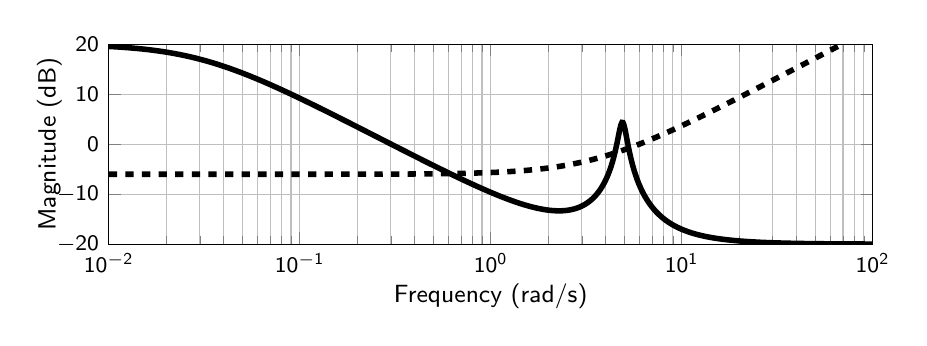
\begin{tikzpicture}

\begin{axis}[%
width=0.8\linewidth,
height=1.0in,
at={(0.71in,0.594in)},
scale only axis,
xmode=log,
xmin=0.01,
xmax=100,
xmajorgrids,
xminorgrids,
ymajorgrids,
xminorticks=true,
xlabel style = {yshift=+1mm},
xlabel={Frequency (rad/s)},
ymin=-20,
ymax=20,
ylabel={Magnitude (dB)},
ylabel style = {yshift=-3mm},
axis background/.style={fill=white}
]
\addplot [color=black,dashed,line width=2.0pt,forget plot]
  table[row sep=crcr]{%
0.01	-6.0205637221138\\
0.0101159111222383	-6.02056287826468\\
0.0102331657833025	-6.02056201473786\\
0.0103517795563018	-6.02056113107649\\
0.0104717681948552	-6.02056022681402\\
0.0105931476351837	-6.02055930146509\\
0.0107159339982267	-6.02055835454007\\
0.0108401435917833	-6.02055738553888\\
0.0109657929126781	-6.02055639394183\\
0.0110928986489522	-6.02055537922514\\
0.0112214776820798	-6.02055434084787\\
0.01135154708921	-6.02055327826044\\
0.0114831241454351	-6.02055219089751\\
0.011616226326085	-6.02055107818058\\
0.0117508713090481	-6.02054993951971\\
0.011887076977119	-6.02054877431116\\
0.0120248614203741	-6.02054758193222\\
0.0121642429385737	-6.02054636175267\\
0.0123052400435926	-6.02054511312162\\
0.0124478714618791	-6.02054383537707\\
0.0125921561369415	-6.02054252784057\\
0.0127381132318648	-6.02054118981788\\
0.0128857621318552	-6.02053982059763\\
0.0130351224468151	-6.02053841945189\\
0.0131862140139475	-6.02053698563679\\
0.0133390569003906	-6.02053551838818\\
0.0134936714058831	-6.0205340169331\\
0.0136500780654601	-6.02053248046758\\
0.0138082976521809	-6.02053090817798\\
0.0139683511798874	-6.02052929922774\\
0.0141302599059953	-6.02052765276282\\
0.0142940453343176	-6.0205259679093\\
0.0144597292179202	-6.02052424377192\\
0.0146273335620113	-6.0205224794336\\
0.014796880626864	-6.02052067395793\\
0.0149683929307726	-6.02051882638569\\
0.0151418932530435	-6.02051693573437\\
0.0153174046370208	-6.02051500100059\\
0.0154949503931463	-6.02051302115661\\
0.015674554102056	-6.02051099515079\\
0.0158562396177114	-6.02050892190599\\
0.0160400310705682	-6.02050680032106\\
0.0162259528707809	-6.0205046292692\\
0.0164140297114447	-6.02050240759739\\
0.0166042865718753	-6.02050013412379\\
0.0167967487209265	-6.02049780764207\\
0.0169914417203463	-6.02049542691682\\
0.0171883914281715	-6.02049299068286\\
0.0173876240021625	-6.0204904976456\\
0.0175891659032773	-6.02048794648034\\
0.0177930438991858	-6.02048533583255\\
0.0179992850678248	-6.02048266431417\\
0.0182079168009946	-6.02047993050787\\
0.0184189668079971	-6.02047713295832\\
0.0186324631193156	-6.02047427018335\\
0.018848434090338	-6.02047134066027\\
0.0190669084051225	-6.02046834283199\\
0.0192879150802078	-6.02046527510619\\
0.0195114834684662	-6.02046213585451\\
0.0197376432630026	-6.02045892340868\\
0.0199664245010979	-6.02045563606262\\
0.0201978575681988	-6.02045227206855\\
0.0204319732019527	-6.02044882964008\\
0.0206688024962908	-6.02044530694919\\
0.0209083769055575	-6.02044170212436\\
0.0211507282486879	-6.02043801325052\\
0.0213958887134342	-6.02043423836804\\
0.0216438908606402	-6.02043037547269\\
0.0218947676285662	-6.02042642250865\\
0.0221485523372636	-6.02042237738026\\
0.0224052786930002	-6.02041823793805\\
0.0226649807927369	-6.02041400198059\\
0.0229276931286565	-6.02040966726023\\
0.0231934505927443	-6.02040523147401\\
0.0234622884814226	-6.0204006922644\\
0.0237342425002387	-6.02039604722103\\
0.0240093487686065	-6.02039129387544\\
0.0242876438246045	-6.02038642970376\\
0.0245691646298279	-6.02038145212337\\
0.024853948574298	-6.02037635848758\\
0.025142033481428	-6.02037114609312\\
0.0254334576130465	-6.02036581216786\\
0.0257282596744793	-6.02036035388215\\
0.0260264788196901	-6.02035476833451\\
0.0263281546564802	-6.02034905255798\\
0.0266333272517498	-6.02034320351756\\
0.0269420371368188	-6.02033721810662\\
0.0272543253128103	-6.02033109314133\\
0.0275702332560958	-6.02032482537474\\
0.0278898029238044	-6.02031841147435\\
0.0282130767593947	-6.02031184803316\\
0.0285400976982924	-6.02030513156493\\
0.0288709091735924	-6.0202982585013\\
0.0292055551218275	-6.02029122519488\\
0.0295440799888038	-6.02028402790843\\
0.0298865287355038	-6.02027666281481\\
0.0302329468440578	-6.02026912600783\\
0.0305833803237843	-6.02026141347946\\
0.0309378757173014	-6.02025352113937\\
0.0312964801067075	-6.02024544478912\\
0.0316592411198352	-6.02023718014063\\
0.0320262069365765	-6.02022872280705\\
0.032397426295282	-6.02022006829446\\
0.0327729484992338	-6.02021121200444\\
0.0331528234231942	-6.02020214923659\\
0.0335371015200293	-6.02019287517319\\
0.0339258338274099	-6.02018338489344\\
0.0343190719745904	-6.02017367335406\\
0.0347168681892656	-6.02016373539552\\
0.0351192753045073	-6.02015356574223\\
0.0355263467657814	-6.02014315899389\\
0.0359381366380463	-6.0201325096196\\
0.0363546996129332	-6.02012161196486\\
0.0367760910160103	-6.0201104602426\\
0.0372023668141307	-6.02009904853116\\
0.0376335836228653	-6.02008737076813\\
0.0380697987140229	-6.0200754207531\\
0.0385110700232557	-6.02006319213651\\
0.038957456157755	-6.02005067842805\\
0.0394090164040345	-6.02003787297949\\
0.0398658107358044	-6.02002476898899\\
0.0403278998219371	-6.0200113595025\\
0.0407953450345245	-6.01999763739224\\
0.0412682084570295	-6.01998359537569\\
0.0417465528925314	-6.01996922599591\\
0.0422304418720667	-6.01995452161759\\
0.0427199396630678	-6.01993947443686\\
0.0432151112778976	-6.01992407646132\\
0.043716022482485	-6.01990831951276\\
0.044222739805059	-6.01989219522675\\
0.0447353305449847	-6.01987569503937\\
0.0452538627817017	-6.01985881019052\\
0.0457784053837662	-6.01984153171044\\
0.0463090280179974	-6.0198238504258\\
0.0468458011587305	-6.01980575694996\\
0.0473887960971765	-6.01978724167396\\
0.0479380849508911	-6.01976829476747\\
0.0484937406733524	-6.01974890616954\\
0.0490558370636505	-6.01972906558336\\
0.0496244487762892	-6.01970876247768\\
0.0501996513311008	-6.01968798607431\\
0.0507815211232767	-6.01966672533459\\
0.0513701354335134	-6.01964496897718\\
0.0519655724382766	-6.0196227054494\\
0.0525679112201842	-6.01959992292906\\
0.0531772317785097	-6.01957660932309\\
0.053793615039807	-6.0195527522523\\
0.0544171428686589	-6.01952833905172\\
0.0550478980785497	-6.01950335676194\\
0.0556859644428641	-6.01947779211832\\
0.0563314267060135	-6.01945163154988\\
0.0569843705946914	-6.01942486117115\\
0.0576448828292588	-6.01939746676991\\
0.0583130511352622	-6.01936943380361\\
0.058988964255085	-6.01934074738969\\
0.0596727119597331	-6.01931139230566\\
0.0603643850607587	-6.01928135296523\\
0.0610640754223204	-6.01925061342687\\
0.0617718759733849	-6.01921915737156\\
0.0624878807200689	-6.01918696810503\\
0.0632121847581246	-6.01915402854203\\
0.0639448842855694	-6.01912032120027\\
0.0646860766154633	-6.01908582818726\\
0.0654358601888324	-6.01905053120069\\
0.0661943345877439	-6.01901441150496\\
0.0669616005485322	-6.01897744993318\\
0.0677377599751775	-6.01893962686908\\
0.0685229159528406	-6.01890092224363\\
0.0693171727615541	-6.01886131551452\\
0.0701206358900718	-6.01882078566426\\
0.07093341204988	-6.018779311192\\
0.0717556091893693	-6.01873687008446\\
0.0725873365081725	-6.01869343982401\\
0.0734287044716677	-6.01864899736993\\
0.0742798248256492	-6.01860351913933\\
0.0751408106111697	-6.01855698100755\\
0.0760117761795533	-6.0185093582796\\
0.0768928372075831	-6.01846062569301\\
0.0777841107128649	-6.01841075739656\\
0.0786857150693685	-6.01835972693469\\
0.0795977700231499	-6.01830750723754\\
0.0805203967082548	-6.01825407060563\\
0.0814537176628075	-6.01819938869534\\
0.0823978568452852	-6.01814343250193\\
0.083352939650982	-6.0180861723483\\
0.0843190929286626	-6.0180275778653\\
0.0852964449974103	-6.01796761797883\\
0.086285125663669	-6.01790626088842\\
0.0872852662384838	-6.01784347405947\\
0.0882969995549409	-6.01777922419519\\
0.0893204599858097	-6.01771347722903\\
0.0903557834613893	-6.0176461982978\\
0.0914031074875623	-6.01757735173326\\
0.0924625711640574	-6.0175069010295\\
0.0935343152029239	-6.01743480884054\\
0.09461848194722	-6.01736103694689\\
0.0957152153899187	-6.01728554624334\\
0.0968246611930312	-6.01720829671247\\
0.097946966706954	-6.0171292474106\\
0.099082280990038	-6.01704835643733\\
0.100230754828387	-6.01696558092342\\
0.101392540755882	-6.01688087700141\\
0.102567793074442	-6.01679419978453\\
0.103756667874519	-6.01670550334215\\
0.104959323055823	-6.01661474067571\\
0.1061759183483	-6.01652186370096\\
0.107406615333343	-6.01642682320794\\
0.108651577465254	-6.016329568847\\
0.10991097009295	-6.01623004910444\\
0.111184960481927	-6.01612821126261\\
0.112473717836475	-6.01602400138224\\
0.113777413322149	-6.01591736427216\\
0.115096220088503	-6.01580824346139\\
0.116430313292088	-6.01569658116372\\
0.117779870119712	-6.01558231825628\\
0.119145069811978	-6.01546539424076\\
0.120526093687084	-6.0153457472167\\
0.121923125164911	-6.01522331384419\\
0.123336349791378	-6.0150980293167\\
0.124765955263087	-6.01496982732821\\
0.126212131452255	-6.01483864002178\\
0.127675070431927	-6.01470439797983\\
0.129154966501488	-6.01456703016912\\
0.130652016212472	-6.01442646390964\\
0.132166418394661	-6.01428262483373\\
0.133698374182495	-6.01413543685624\\
0.135248087041788	-6.013984822121\\
0.136815762796747	-6.01383070097416\\
0.138401609657313	-6.01367299191178\\
0.14000583824681	-6.01351161154245\\
0.14162866162992	-6.01334647454185\\
0.143270295340983	-6.01317749361237\\
0.144930957412622	-6.01300457943185\\
0.146610868404698	-6.01282764061204\\
0.14831025143361	-6.01264658364727\\
0.150029332201922	-6.01246131286592\\
0.151768339028341	-6.01227173038665\\
0.153527502878042	-6.01207773605987\\
0.155307057393346	-6.01187922741967\\
0.157107238924745	-6.01167609963186\\
0.158928286562298	-6.01146824543075\\
0.160770442167382	-6.01125555508047\\
0.162633950404819	-6.01103791630244\\
0.164519058775366	-6.01081521422132\\
0.16642601764859	-6.01058733131452\\
0.16835508029612	-6.01035414733488\\
0.170306502925284	-6.01011553926432\\
0.172280544713139	-6.00987138123969\\
0.174277467840892	-6.0096215444948\\
0.176297537528721	-6.00936589729117\\
0.178341022071001	-6.00910430484639\\
0.180408192871938	-6.00883662927267\\
0.182499324481615	-6.00856272949916\\
0.184614694632455	-6.00828246120154\\
0.186754584276108	-6.00799567672991\\
0.188919277620767	-6.00770222502928\\
0.191109062168914	-6.00740195156513\\
0.193324228755505	-6.00709469824241\\
0.195565071586595	-6.00678030332572\\
0.197831888278416	-6.0064586013557\\
0.200124979896904	-6.00612942306464\\
0.20244465099768	-6.0057925952892\\
0.204791209666509	-6.00544794088614\\
0.207164967560207	-6.00509527863432\\
0.209566239948043	-6.00473442314948\\
0.211995345753607	-6.00436518478912\\
0.214452607597167	-6.0039873695484\\
0.216938351838518	-6.00360077897462\\
0.219452908620331	-6.00320521005007\\
0.221996611911995	-6.00280045511194\\
0.224569799553977	-6.00238630172091\\
0.227172813302691	-6.00196253256971\\
0.229805998875885	-6.00152892537851\\
0.232469705998565	-6.00108525276438\\
0.235164288449435	-6.00063128214071\\
0.237890104107889	-6.0001667755956\\
0.240647515001542	-5.99969148977542\\
0.243436887354311	-5.99920517575911\\
0.246258591635055	-5.99870757893169\\
0.249113002606779	-5.99819843886596\\
0.252000499376409	-5.99767748918086\\
0.254921465445142	-5.99714445741767\\
0.25787628875938	-5.99659906489376\\
0.260865361762255	-5.9960410265809\\
0.263889081445751	-5.9954700509444\\
0.266947849403432	-5.99488583981254\\
0.270042071883777	-5.99428808822343\\
0.273172159844138	-5.9936764842736\\
0.276338529005317	-5.99305070896736\\
0.279541599906786	-5.99241043605417\\
0.282781797962534	-5.99175533187249\\
0.286059553517574	-5.99108505519036\\
0.289375301905095	-5.99039925702582\\
0.292729483504282	-5.98969758049047\\
0.296122543798803	-5.98897966060395\\
0.299554933435981	-5.98824512412347\\
0.30302710828664	-5.98749358935508\\
0.306539529505653	-5.98672466597684\\
0.310092663593193	-5.98593795485237\\
0.313686982456688	-5.98513304782005\\
0.317322963473498	-5.98430952752041\\
0.321001089554317	-5.9834669671765\\
0.324721849207313	-5.98260493039667\\
0.328485736603004	-5.98172297097329\\
0.332293251639897	-5.98082063265578\\
0.336144900010876	-5.97989744894394\\
0.340041193270371	-5.97895294285932\\
0.343982648902292	-5.97798662673387\\
0.347969790388769	-5.97699800195598\\
0.352003147279668	-5.97598655876097\\
0.356083255262928	-5.97495177597501\\
0.360210656235707	-5.97389312077893\\
0.364385898376354	-5.97281004846045\\
0.368609536217216	-5.97170200215393\\
0.372882130718284	-5.97056841259293\\
0.3772042493417	-5.96940869783638\\
0.381576466127125	-5.96822226301434\\
0.385999361767977	-5.96700850004139\\
0.390473523688556	-5.96576678734746\\
0.394999546122065	-5.96449648959481\\
0.399578030189527	-5.96319695738595\\
0.404209583979631	-5.96186752697319\\
0.408894822629486	-5.96050751996194\\
0.413634368406328	-5.9591162430019\\
0.418428850790158	-5.9576929874846\\
0.423278906557355	-5.95623702922472\\
0.428185179865241	-5.95474762813902\\
0.43314832233764	-5.95322402792058\\
0.438168993151419	-5.95166545571636\\
0.44324785912404	-5.95007112177576\\
0.448385594802119	-5.94844021912563\\
0.453582882551019	-5.94677192320176\\
0.458840412645476	-5.94506539151446\\
0.464158883361278	-5.94331976327635\\
0.469539001068006	-5.94153415904673\\
0.47498148032285	-5.93970768034789\\
0.480487043965513	-5.93783940930173\\
0.486056423214214	-5.93592840823639\\
0.491690357762803	-5.93397371930062\\
0.497389595879007	-5.93197436407808\\
0.503154894503805	-5.9299293431707\\
0.508987019351968	-5.92783763580811\\
0.51488674501375	-5.92569819942417\\
0.520854855057766	-5.92350996924421\\
0.526892142135067	-5.92127185786347\\
0.532999408084409	-5.91898275481123\\
0.53917746403875	-5.91664152612462\\
0.545427130532983	-5.91424701389454\\
0.551749237612913	-5.9117980358379\\
0.558144624945496	-5.90929338482372\\
0.564614141930367	-5.90673182843525\\
0.571158647812643	-5.90411210849294\\
0.57777901179705	-5.90143294059619\\
0.584476113163363	-5.89869301364059\\
0.591250841383188	-5.89589098934364\\
0.598104096238094	-5.89302550176626\\
0.605036787939122	-5.89009515681134\\
0.61204983724767	-5.88709853174245\\
0.619144175597784	-5.88403417468461\\
0.626320745219869	-5.88090060410718\\
0.633580499265825	-5.87769630833995\\
0.640924401935645	-5.87441974504404\\
0.648353428605472	-5.87106934070098\\
0.655868565957143	-5.86764349010964\\
0.663470812109235	-5.86414055583882\\
0.671161176749628	-5.86055886772439\\
0.678940681269611	-5.8568967223284\\
0.68681035889953	-5.85315238241566\\
0.694771254846024	-5.84932407642042\\
0.702824426430835	-5.84540999790651\\
0.710970943231243	-5.84140830504204\\
0.719211887222119	-5.8373171200511\\
0.727548352919623	-5.83313452868083\\
0.735981447526577	-5.82885857966426\\
0.744512291079514	-5.82448728417673\\
0.753142016597437	-5.82001861530683\\
0.761871770232299	-5.81545050750771\\
0.77070271142123	-5.81078085607245\\
0.779636013040523	-5.80600751659076\\
0.788672861561415	-5.80112830442523\\
0.797814457207663	-5.79614099418411\\
0.80706201411495	-5.79104331918753\\
0.816416760492147	-5.78583297095606\\
0.825879938784427	-5.78050759869389\\
0.835452805838287	-5.77506480877971\\
0.845136633068472	-5.76950216425851\\
0.854932706626838	-5.76381718435919\\
0.864842327573172	-5.75800734399037\\
0.874866812047991	-5.75207007327027\\
0.885007491447343	-5.74600275706053\\
0.89526571259964	-5.73980273449954\\
0.905642837944529	-5.73346729856013\\
0.916140245713852	-5.7269936956114\\
0.926759330114688	-5.72037912499844\\
0.937501501514528	-5.71362073863375\\
0.948368186628592	-5.70671564060676\\
0.959360828709314	-5.69966088680434\\
0.97048088773803	-5.69245348455718\\
0.981729840618884	-5.68509039229382\\
0.99310918137498	-5.67756851922937\\
1.00462042134681	-5.66988472505412\\
1.016265089393	-5.66203581967021\\
1.02804473209331	-5.65401856292998\\
1.03996091395412	-5.6458296644101\\
1.05201521761616	-5.63746578320748\\
1.06420924406472	-5.62892352776461\\
1.07654461284232	-5.62019945573108\\
1.08902296226373	-5.61129007383567\\
1.10164594963366	-5.60219183781382\\
1.11441525146679	-5.59290115234588\\
1.12733256371049	-5.5834143710509\\
1.14039960197003	-5.57372779650784\\
1.15361810173648	-5.56383768030305\\
1.16698981861715	-5.55374022313423\\
1.18051652856881	-5.5434315749563\\
1.19420002813353	-5.53290783514867\\
1.20804213467733	-5.52216505274889\\
1.22204468663149	-5.5111992267234\\
1.23620954373677	-5.50000630628139\\
1.25053858729039	-5.48858219124835\\
1.2650337203959	-5.47692273247814\\
1.27969686821594	-5.46502373232976\\
1.29452997822792	-5.45288094518069\\
1.30953502048267	-5.44049007802373\\
1.32471398786612	-5.42784679108642\\
1.34006889636395	-5.41494669853441\\
1.35560178532937	-5.40178536923265\\
1.37131471775395	-5.38835832754869\\
1.38720978054162	-5.37466105425037\\
1.40328908478587	-5.36068898743755\\
1.4195547660501	-5.34643752355992\\
1.43600898465126	-5.33190201849641\\
1.45265392594678	-5.31707778870537\\
1.46949180062482	-5.30196011243408\\
1.48652484499786	-5.28654423101739\\
1.50375532129974	-5.2708253502347\\
1.5211855179861	-5.25479864174972\\
1.53881775003835	-5.23845924461158\\
1.55665435927106	-5.22180226684959\\
1.57469771464309	-5.20482278712939\\
1.59295021257212	-5.18751585648841\\
1.61141427725302	-5.16987650015707\\
1.63009236097974	-5.15189971944385\\
1.64898694447107	-5.13358049371246\\
1.66810053720006	-5.11491378242684\\
1.68743567772738	-5.09589452727693\\
1.70699493403841	-5.07651765438521\\
1.72678090388436	-5.05677807659204\\
1.74679621512725	-5.03667069581064\\
1.76704352608895	-5.01619040546547\\
1.78752552590424	-4.99533209300539\\
1.80824493487795	-4.97409064249599\\
1.82920450484629	-4.95246093727136\\
1.8504070195423	-4.93043786267913\\
1.87185529496558	-4.90801630887984\\
1.8935521797563	-4.88519117372392\\
1.91550055557353	-4.86195736569572\\
1.93770333747799	-4.83830980692042\\
1.96016347431919	-4.81424343623524\\
1.98288394912707	-4.78975321232693\\
2.00586777950823	-4.76483411691415\\
2.02911801804668	-4.73948115800178\\
2.05263775270925	-4.71368937317039\\
2.07643010725577	-4.68745383292742\\
2.10049824165392	-4.66076964410288\\
2.12484535249888	-4.63363195327084\\
2.14947467343798	-4.6060359502284\\
2.17438947560008	-4.57797687149736\\
2.19959306803007	-4.54945000385936\\
2.22508879812837	-4.52045068790537\\
2.25088005209546	-4.49097432162002\\
2.27697025538168	-4.46101636396974\\
2.30336287314213	-4.43057233850463\\
2.33006141069692	-4.39963783696316\\
2.35706941399673	-4.3682085228805\\
2.38439047009372	-4.33628013518202\\
2.41202820761801	-4.30384849177277\\
2.43998629725955	-4.27090949310823\\
2.46826845225569	-4.23745912573519\\
2.49687842888433	-4.2034934658123\\
2.52582002696278	-4.16900868258559\\
2.55509709035251	-4.13400104183211\\
2.58471350746956	-4.09846690924719\\
2.61467321180109	-4.06240275378364\\
2.64498018242772	-4.02580515092955\\
2.67563844455205	-3.98867078591746\\
2.70665207003324	-3.95099645686996\\
2.73802517792786	-3.9127790778528\\
2.76976193503689	-3.87401568185626\\
2.8018665564592	-3.83470342368508\\
2.83434330615131	-3.79483958274472\\
2.86719649749377	-3.75442156573529\\
2.90043049386399	-3.71344690923429\\
2.93404970921579	-3.67191328216772\\
2.9680586086656	-3.6298184881632\\
3.00246170908555	-3.58716046778369\\
3.03726357970331	-3.54393730062898\\
3.072468842709	-3.5001472073113\\
3.10808217386906	-3.45578855129232\\
3.14410830314726	-3.41085984058201\\
3.18055201533292	-3.36535972928748\\
3.21741815067637	-3.31928701902595\\
3.25471160553185	-3.27264066017842\\
3.29243733300777	-3.22541975299608\\
3.33060034362459	-3.17762354854876\\
3.36920570598027	-3.12925144951673\\
3.40825854742345	-3.08030301081933\\
3.44776405473446	-3.0307779400969\\
3.48772747481418	-2.98067609801131\\
3.52815411538088	-2.92999749839618\\
3.56904934567523	-2.87874230824775\\
3.61041859717334	-2.82691084754015\\
3.65226736430818	-2.77450358889168\\
3.6946012051993	-2.72152115706026\\
3.73742574239106	-2.66796432828443\\
3.78074666359935	-2.61383402946053\\
3.824569722467	-2.55913133717095\\
3.86890073932798	-2.50385747654498\\
3.91374560198038	-2.44801381997815\\
3.95911026646846	-2.39160188570039\\
4.00500075787361	-2.33462333619289\\
4.05142317111465	-2.27707997646521\\
4.09838367175726	-2.21897375219603\\
4.14588849683291	-2.16030674773203\\
4.19394395566719	-2.10108118396439\\
4.24255643071778	-2.04129941607345\\
4.29173237842216	-1.98096393115055\\
4.34147833005509	-1.92007734570932\\
4.39180089259609	-1.85864240308258\\
4.44270674960688	-1.7966619707121\\
4.49420266211914	-1.73413903733982\\
4.5462954695324	-1.67107671010458\\
4.59899209052244	-1.60747821154795\\
4.65229952396019	-1.54334687654004\\
4.70622484984128	-1.47868614912649\\
4.76077523022637	-1.41349957930294\\
4.81595791019235	-1.34779081972886\\
4.87178021879463	-1.28156362237763\\
4.92824957004051	-1.21482183513854\\
4.98537346387389	-1.14756939836867\\
5.04315948717136	-1.07981034140628\\
5.10161531474983	-1.01154877905026\\
5.16074871038591	-0.942788908008469\\
5.22056752784698	-0.873535003325574\\
5.28107971193433	-0.803791414796166\\
5.34229329953835	-0.733562563360863\\
5.40421642070591	-0.6628529375052\\
5.46685729972018	-0.59166708965005\\
5.5302242561929	-0.520009632556332\\
5.59432570616938	-0.447885235730966\\
5.65917016324624	-0.375298621858242\\
5.72476623970218	-0.302254563243426\\
5.79112264764176	-0.228757878287007\\
5.85824820015254	-0.154813427985333\\
5.92615181247555	-0.0804261124688321\\
5.99484250318941	-0.00560086757568178\\
6.06432939540806	0.0696573385349038\\
6.13462171799251	0.145343508714662\\
6.2057288067765	0.221452620120421\\
6.2776601058065	0.2979796274458\\
6.35042516859596	0.37491946610353\\
6.42403365939419	0.452267055347856\\
6.49849535446989	0.530017301331814\\
6.57382014340959	0.608165100107739\\
6.65001803043112	0.686705340554985\\
6.72709913571234	0.765632907245258\\
6.80507369673521	0.844942683234003\\
6.8839520696455	0.924629552781127\\
6.96374473062822	1.00468840400298\\
7.04446227729904	1.08511413144244\\
7.12611543011175	1.16590163857112\\
7.20871503378214	1.24704584021129\\
7.29227205872831	1.32854166488035\\
7.37679760252773	1.41038405706169\\
7.46230289139111	1.4925679793952\\
7.54879928165343	1.57508841478746\\
7.63629826128224	1.65794036844815\\
7.7248114514034	1.74111886984686\\
7.81435060784454	1.82461897458903\\
7.90492762269642	1.90843576621908\\
7.99655452589235	1.99256435794264\\
8.08924348680594	2.07699989427502\\
8.18300681586739	2.16173755261046\\
8.27785696619847	2.24677254472023\\
8.37380653526649	2.33210011817197\\
8.4708682665574	2.41771555768179\\
8.56905505126835	2.50361418638688\\
8.66837993001977	2.5897913670532\\
8.76885609458743	2.67624250321064\\
8.8704968896544	2.76296304021882\\
8.97331581458352	2.84994846626764\\
9.07732652521022	2.93719431331039\\
9.18254283565628	3.02469615793278\\
9.2889787201645	3.11244962215954\\
9.39664831495469	3.20045037419869\\
9.50556592010119	3.28869412912605\\
9.6157460014321	3.3771766495124\\
9.72720319245054	3.46589374599101\\
9.83995229627823	3.5548412777743\\
9.95400828762152	3.64401515311205\\
10.0693863147603	3.73341132970179\\
10.1861017015598	3.82302581504534\\
10.3041699495059	3.91285466676006\\
10.423606739764	4.00289399283968\\
10.5444279352617	4.09313995187269\\
10.6666495827954	4.18358875321359\\
10.7902879151618	4.27423665711524\\
10.9153593533139	4.36507997481844\\
11.0418805085416	4.45611506860283\\
11.1698681846782	4.54733835180025\\
11.2993393803322	4.63874628877294\\
11.4303112911448	4.73033539485636\\
11.5628013120738	4.82210223626817\\
11.6968270397038	4.91404342998881\\
11.8324062745838	5.00615564360848\\
11.9695570235904	5.09843559514708\\
12.1082975023204	5.19088005284786\\
12.2486461375093	5.28348583494298\\
12.3906215694792	5.37624980939627\\
12.534242654614	5.4691688936215\\
12.6795284678643	5.56224005417968\\
12.8264983052806	5.65546030645467\\
12.9751716865759	5.74882671430987\\
13.1255683577184	5.842336389726\\
13.2777082935543	5.93598649242139\\
13.4316117004602	6.029774229457\\
13.5872990190271	6.12369685482553\\
13.7447909267754	6.21775166902624\\
13.9041083409007	6.31193601862725\\
14.0652724210524	6.40624729581582\\
14.2283045721435	6.50068293793602\\
14.3932264471941	6.59524042701833\\
14.5600599502065	6.68991728929765\\
14.728827239075	6.7847110947239\\
14.8995507285286	6.8796194564645\\
15.0722530931076	6.97464003039983\\
15.2469572701757	7.06977051461231\\
15.4236864629663	7.16500864886995\\
15.6024641436637	7.26035221410533\\
15.7833140565212	7.35579903188963\\
15.9662602210143	7.45134696390352\\
16.1513269350309	7.54699391140518\\
16.3385387780986	7.64273781469561\\
16.527920614649	7.73857665258205\\
16.7194975973199	7.83450844183995\\
16.9132951702965	7.93053123667458\\
17.1093390726902	8.02664312818179\\
17.3076553419573	8.1228422438085\\
17.5082703173573	8.21912674681468\\
17.7112106434509	8.31549483573518\\
17.916503273639	8.41194474384365\\
18.1241754737424	8.50847473861732\\
18.3342548256229	8.6050831212045\\
18.546769230847	8.70176822589391\\
18.7617469143912	8.7985284195867\\
18.979216428391	8.89536210127139\\
19.1992066559328	8.9922677015022\\
19.4217468148903	9.08924368188027\\
19.6468664618045	9.18628853453914\\
19.8745954958098	9.28340078163351\\
20.104964162605	9.38057897483267\\
20.3380030584698	9.47782169481762\\
20.5737431343291	9.57512755078313\\
20.8122156998634	9.67249517994398\\
21.0534524276671	9.76992324704642\\
21.2974853574552	9.86741044388395\\
21.5443469003188	9.96495548881876\\
21.7940698430296	10.0625571263078\\
22.0466873523941	10.1602141264342\\
22.3022329796594	10.2579252844446\\
22.5607406649686	10.3556894202906\\
22.822244741869	10.4535053781774\\
23.0867799418717	10.5513720261164\\
23.3543813990648	10.6492882554848\\
23.6250846547795	10.7472529805895\\
23.8989256623105	10.8452651382382\\
24.1759407916913	10.9433236873149\\
24.4561668345245	11.041427608362\\
24.7396410088681	11.139575903168\\
25.0264009641792	11.2377675943606\\
25.3164847863136	11.3360017250067\\
25.6099310025846	11.4342773582169\\
25.9067785868801	11.5325935767565\\
26.2070669648385	11.6309494826622\\
26.5108360190854	11.7293441968653\\
26.8181260945302	11.8277768588189\\
27.1289780037247	11.926246626133\\
27.4434330322837	12.0247526742136\\
27.761532944368	12.1232941959088\\
28.0833199882317	12.2218704011596\\
28.408836901833	12.3204805166568\\
28.7381269185107	12.4191237855037\\
29.0712337727258	12.517799466884\\
29.4082017058706	12.6165068357352\\
29.7490754721444	12.7152451824277\\
30.0939003444972	12.8140138124493\\
30.442722120643	12.9128120460951\\
30.7955871291423	13.0116392181625\\
31.1525422355549	13.1104946776513\\
31.5136348486648	13.2093777874701\\
31.8789129267765	13.3082879241463\\
32.2484249840844	13.4072244775424\\
32.6222200971167	13.5061868505768\\
33.0003479112529	13.6051744589496\\
33.3828586473176	13.7041867308736\\
33.7698031082509	13.8032231068098\\
34.1612326858553	13.9022830392078\\
34.5571993676214	14.0013659922511\\
34.9577557436328	14.1004714416068\\
35.3629550135504	14.1995988741801\\
35.7728509936787	14.2987477878733\\
36.1874981241128	14.3979176913489\\
36.606951475969	14.4971081037979\\
37.0312667586993	14.5963185547114\\
37.4605003274899	14.6955485836576\\
37.8947091907467	14.7947977400616\\
38.333951017666	14.894065582991\\
38.7782841458946	14.993351680944\\
39.2277675892772	15.0926556116427\\
39.6824610456948	15.1919769618293\\
40.1424249049932	15.2913153270671\\
40.6077202570037	15.3906703115447\\
41.0784088996565	15.4900415278843\\
41.5545533471888	15.5894285969532\\
42.0362168384471	15.6888311476795\\
42.5234633452868	15.7882488168706\\
43.016357581068	15.8876812490362\\
43.5149650092505	15.9871280962138\\
44.0193518520887	16.0865890177977\\
44.5295850994266	16.1860636803718\\
45.0457325175946	16.2855517575452\\
45.5678626584106	16.3850529297911\\
46.0960448682843	16.4845668842884\\
46.6303492974273	16.5840933147673\\
47.1708469091702	16.6836319213568\\
47.7176094893875	16.783182410436\\
48.2707096560318	16.8827444944875\\
48.8302208687788	16.9823178919543\\
49.3962174387832	17.0819023270992\\
49.9687745385488	17.1814975298663\\
50.5479682119124	17.2811032357465\\
51.1338753841433	17.3807191856441\\
51.7265738721602	17.480345125747\\
52.3261423948666	17.5799808073988\\
52.9326605836056	17.6796259869736\\
53.5462089927361	17.7792804257529\\
54.1668691103315	17.8789438898053\\
54.7947233690029	17.9786161498679\\
55.4298551568467	18.0782969812301\\
56.0723488285203	18.1779861636202\\
56.7222897164454	18.277683481093\\
57.3797641421413	18.37738872192\\
58.0448594276898	18.4771016784822\\
58.7176639073326	18.576822147164\\
59.3982669392036	18.6765499282491\\
60.0867589171969	18.7762848258191\\
60.7832312829723	18.8760266476529\\
61.4877765381002	18.9757752051287\\
62.2004882563471	19.0755303131272\\
62.9214610961034	19.1752917899367\\
63.6507908129557	19.2750594571601\\
64.3885742724042	19.374833139623\\
65.134909462728	19.4746126652839\\
65.8898955079995	19.5743978651455\\
66.6536326812491	19.6741885731679\\
67.4262224177834	19.7739846261829\\
68.2077673286569	19.8737858638097\\
68.9983712143002	19.9735921283726\\
69.7981390783066	20.0734032648189\\
70.6071771413777	20.1732191206394\\
71.4255928554313	20.273039545789\\
72.2534949178721	20.3728643926093\\
73.0909932860291	20.472693515752\\
73.9381991917587	20.5725267721037\\
74.7952251562182	20.6723640207112\\
75.6621850048106	20.7722051227091\\
76.5391938823015	20.8720499412469\\
77.4263682681127	20.9718983414185\\
78.323825991792	21.0717501901916\\
79.2316862486625	21.1716053563387\\
80.150069615654	21.2714637103686\\
81.0790980673169	21.3713251244592\\
82.018894992022	21.4711894723908\\
82.9695852083491	21.5710566294802\\
83.9312949816636	21.6709264725156\\
84.9041520408875	21.7707988796926\\
85.8882855954625	21.8706737305501\\
86.8838263525118	21.9705509059079\\
87.8909065341995	22.0704302878042\\
88.9096598952916	22.1703117594336\\
89.9402217409204	22.2701952050867\\
90.9827289445556	22.370080510089\\
92.0373199661822	22.4699675607411\\
93.1041348706908	22.5698562442591\\
94.1833153464795	22.6697464487155\\
95.2750047242729	22.7696380629809\\
96.3793479961579	22.8695309766654\\
97.4964918348409	22.9694250800606\\
98.6265846131282	23.0693202640827\\
99.769776423632	23.1692164202149\\
100.926219098705	23.2691134404502\\
102.096066230605	23.3690112172356\\
103.279473191895	23.4689096434146\\
104.476597156081	23.568808612172\\
105.687597118481	23.6687080169772\\
106.912633917348	23.7686077515284\\
108.151870255229	23.868507709697\\
109.405470720574	23.9684077854716\\
110.673601809597	24.0683078729028\\
111.956431948388	24.1682078660472\\
113.254131515281	24.2681076589117\\
114.566872863487	24.3680071453985\\
115.894830343981	24.4679062192486\\
117.23818032866	24.5678047739866\\
118.597101233767	24.6677027028645\\
119.971773543589	24.767599898806\\
121.362379834424	24.86749625435\\
122.769104798836	24.9673916615945\\
124.192135270178	25.0672860121395\\
125.631660247412	25.167179197031\\
127.087870920206	25.267071106703\\
128.56096069433	25.3669616309205\\
130.051125217341	25.4668506587219\\
131.558562404571	25.5667380783601\\
133.083472465408	25.666623777245\\
134.626057929891	25.7665076418836\\
136.186523675608	25.8663895578213\\
137.765076954906	25.9662694095813\\
139.361927422414	26.0661470806049\\
140.977287162897	26.16602245319\\
142.611370719413	26.2658954084297\\
144.264395121816	26.3657658261504\\
145.936579915576	26.4656335848486\\
147.628147190939	26.5654985616277\\
149.339321612425	26.665360632134\\
151.070330448666	26.7652196704913\\
152.821403602587	26.865075549236\\
154.592773641948	26.96492813925\\
156.384675830225	27.0647773096936\\
158.19734815786	27.1646229279378\\
160.03103137387	27.2644648594946\\
161.88596901782	27.3643029679477\\
163.762407452169	27.4641371148809\\
165.660595894992	27.5639671598071\\
167.580786453077	27.6637929600944\\
169.523234155412	27.7636143708928\\
171.488196987054	27.8634312450589\\
173.475935923393	27.9632434330793\\
175.486714964815	28.0630507829938\\
177.520801171764	28.1628531403164\\
179.57846470021	28.2626503479554\\
181.659978837533	28.3624422461326\\
183.765620038817	28.4622286723001\\
185.895667963569	28.5620094610575\\
188.050405512858	28.6617844440655\\
190.230118866895	28.7615534499603\\
192.435097523033	28.8613163042645\\
194.665634334226	28.961072829298\\
196.922025547917	29.0608228440866\\
199.204570845387	29.1605661642688\\
201.513573381556	29.260302602002\\
203.849339825246	29.3600319658654\\
206.212180399914	29.4597540607627\\
208.60240892485	29.5594686878224\\
211.02034285686	29.6591756442956\\
213.466303332425	29.7588747234533\\
215.940615210357	29.8585657144807\\
218.443607114943	29.9582484023698\\
220.97561147959	30.0579225678105\\
223.53696459098	30.1575879870789\\
226.128006633728	30.2572444319237\\
228.74908173557	30.3568916694509\\
231.400538013065	30.4565294620058\\
234.082727617829	30.556157567053\\
236.796006783308	30.6557757370537\\
239.540735872088	30.7553837193413\\
242.31727942376	30.8549812559939\\
245.126006203334	30.954568083705\\
247.967289250216	31.054143933651\\
250.841505927754	31.1537085313566\\
253.749037973357	31.2532615965575\\
256.690271549195	31.3528028430603\\
259.665597293487	31.4523319785997\\
262.675410372384	31.5518487046927\\
265.720110532451	31.6513527164906\\
268.800102153761	31.7508437026274\\
271.915794303602	31.8503213450653\\
275.067600790807	31.9497853189377\\
278.255940220713	32.0492352923885\\
281.481236050758	32.1486709264085\\
284.743916646725	32.2480918746687\\
288.04441533963	32.3474977833501\\
291.383170483279	32.4468882909705\\
294.760625512486	32.5462630282072\\
298.177229001967	32.6456216177172\\
301.63343472592	32.7449636739531\\
305.129701718287	32.8442888029758\\
308.666494333727	32.9435966022635\\
312.244282309286	33.0428866605165\\
315.863540826782	33.1421585574593\\
319.524750575921	33.2414118636376\\
323.228397818138	33.3406461402122\\
326.974974451177	33.4398609387487\\
330.764978074424	33.539055801003\\
334.598912054997	33.638230258703\\
338.477285594598	33.7373838333257\\
342.400613797143	33.8365160358704\\
346.369417737173	33.9356263666275\\
350.384224529068	34.0347143149428\\
354.445567397044	34.1337793589775\\
358.553985745982	34.2328209654635\\
362.710025233065	34.3318385894543\\
366.914237840249	34.4308316740714\\
371.167181947577	34.5297996502453\\
375.469422407334	34.6287419364529\\
379.821530619074	34.7276579384487\\
384.224084605506	34.826547048992\\
388.677669089267	34.9254086475693\\
393.182875570577	35.0242421001105\\
397.740302405804	35.1230467587016\\
402.350554886929	35.221821961291\\
407.014245321944	35.3205670313911\\
411.731993116168	35.4192812777747\\
416.504424854519	35.5179639941661\\
421.332174384729	35.6166144589262\\
426.215882901533	35.7152319347336\\
431.156199031823	35.8138156682585\\
436.153778920801	35.9123648898323\\
441.209286319119	36.0108788131114\\
446.32339267104	36.1093566347351\\
451.49677720361	36.2077975339782\\
456.730127016875	36.3062006723975\\
462.024137175131	36.4045651934732\\
467.379510799246	36.5028902222441\\
472.796959160039	36.6011748649372\\
478.277201772749	36.6994182085917\\
483.820966492596	36.7976193206766\\
489.428989611453	36.8957772487032\\
495.102015955635	36.9938910198316\\
500.840798984821	37.0919596404708\\
506.646100892127	37.1899820958742\\
512.518692705333	37.2879573497275\\
518.459354389291	37.3858843437329\\
524.468874949512	37.4837619971857\\
530.548052536957	37.5815892065462\\
536.697694554048	37.6793648450055\\
542.918617761894	37.7770877620459\\
549.211648388779	37.874756782995\\
555.577622239888	37.9723707085752\\
562.017384808319	38.0699283144469\\
568.531791387375	38.1674283507465\\
575.121707184161	38.2648695416191\\
581.788007434494	38.3622505847462\\
588.531577519145	38.4595701508674\\
595.353313081437	38.5568268832982\\
602.254120146193	38.6540193974415\\
609.234915240071	38.7511462802961\\
616.296625513294	38.8482060899586\\
623.440188862786	38.9451973551222\\
630.666554056741	39.0421185745708\\
637.976680860628	39.1389682166689\\
645.37154016467	39.2357447188472\\
652.852114112785	39.3324464870855\\
660.419396233031	39.4290718953913\\
668.074391569562	39.5256192852755\\
675.818116816111	39.6220869652246\\
683.651600451024	39.7184732101717\\
691.575882873852	39.8147762609631\\
699.592016543538	39.9109943238246\\
707.701066118189	40.0071255698249\\
715.904108596489	40.1031681343386\\
724.202233460732	40.1991201165073\\
732.596542821523	40.2949795787008\\
741.088151564157	40.3907445459779\\
749.678187496688	40.4864130055476\\
758.367791499719	40.5819829062309\\
767.15811767793	40.6774521579239\\
776.050333513357	40.7728186310626\\
785.045620020451	40.8680801560907\\
794.145171902934	40.963234522929\\
803.350197712473	41.0582794804492\\
812.661920009195	41.1532127359521\\
822.081575524054	41.2480319546491\\
831.610415323096	41.3427347591509\\
841.249704973612	41.4373187289612\\
851.000724712225	41.5317813999773\\
860.864769614924	41.6261202639989\\
870.843149769072	41.7203327682453\\
880.937190447399	41.8144163148809\\
891.14823228402	41.9083682605521\\
901.477631452492	42.0021859159345\\
911.92675984593	42.0958665452922\\
922.497005259217	42.1894073660498\\
933.189771573324	42.2828055483788\\
944.00647894176	42.3760582147986\\
954.948563979197	42.469162439793\\
966.017479952265	42.5621152494448\\
977.214696972572	42.6549136210878\\
988.541702191957	42.7475544829781\\
1000	42.8400347139869\\
};
\label{line:w1};
\addplot [color=black,solid,line width=2.0pt,forget plot]
  table[row sep=crcr]{%
0.01	19.5425093444695\\
0.0101159111222383	19.5323968347539\\
0.0102331657833025	19.5220728646974\\
0.0103517795563018	19.5115335306464\\
0.0104717681948552	19.5007748786482\\
0.0105931476351837	19.4897929047271\\
0.0107159339982267	19.4785835552071\\
0.0108401435917833	19.4671427270836\\
0.0109657929126781	19.4554662684467\\
0.0110928986489522	19.4435499789562\\
0.0112214776820798	19.4313896103708\\
0.01135154708921	19.4189808671335\\
0.0114831241454351	19.4063194070134\\
0.011616226326085	19.3934008418069\\
0.0117508713090481	19.3802207380992\\
0.011887076977119	19.3667746180875\\
0.0120248614203741	19.353057960468\\
0.0121642429385737	19.3390662013874\\
0.0123052400435926	19.3247947354608\\
0.0124478714618791	19.3102389168574\\
0.0125921561369415	19.2953940604548\\
0.0127381132318648	19.280255443064\\
0.0128857621318552	19.2648183047257\\
0.0130351224468151	19.2490778500782\\
0.0131862140139475	19.2330292498006\\
0.0133390569003906	19.2166676421286\\
0.0134936714058831	19.1999881344471\\
0.0136500780654601	19.1829858049578\\
0.0138082976521809	19.1656557044247\\
0.0139683511798874	19.1479928579957\\
0.0141302599059953	19.1299922671027\\
0.0142940453343176	19.1116489114394\\
0.0144597292179202	19.0929577510173\\
0.0146273335620113	19.0739137283001\\
0.014796880626864	19.0545117704157\\
0.0149683929307726	19.0347467914464\\
0.0151418932530435	19.0146136947965\\
0.0153174046370208	18.9941073756361\\
0.0154949503931463	18.9732227234217\\
0.015674554102056	18.9519546244911\\
0.0158562396177114	18.9302979647327\\
0.0160400310705682	18.9082476323272\\
0.0162259528707809	18.8857985205605\\
0.0164140297114447	18.862945530706\\
0.0166042865718753	18.839683574974\\
0.0167967487209265	18.8160075795274\\
0.0169914417203463	18.7919124875595\\
0.0171883914281715	18.7673932624332\\
0.0173876240021625	18.7424448908773\\
0.0175891659032773	18.7170623862385\\
0.0177930438991858	18.6912407917847\\
0.0179992850678248	18.6649751840566\\
0.0182079168009946	18.6382606762648\\
0.0184189668079971	18.6110924217275\\
0.0186324631193156	18.5834656173455\\
0.018848434090338	18.5553755071099\\
0.0190669084051225	18.5268173856394\\
0.0192879150802078	18.4977866017404\\
0.0195114834684662	18.4682785619872\\
0.0197376432630026	18.4382887343165\\
0.0199664245010979	18.4078126516315\\
0.0201978575681988	18.3768459154093\\
0.0204319732019527	18.3453841993084\\
0.0206688024962908	18.3134232527681\\
0.0209083769055575	18.2809589045966\\
0.0211507282486879	18.2479870665403\\
0.0213958887134342	18.2145037368291\\
0.0216438908606402	18.1805050036925\\
0.0218947676285662	18.1459870488388\\
0.0221485523372636	18.1109461508931\\
0.0224052786930002	18.0753786887867\\
0.0226649807927369	18.0392811450926\\
0.0229276931286565	18.0026501093006\\
0.0231934505927443	17.9654822810259\\
0.0234622884814226	17.9277744731455\\
0.0237342425002387	17.8895236148553\\
0.0240093487686065	17.850726754644\\
0.0242876438246045	17.8113810631754\\
0.0245691646298279	17.7714838360752\\
0.024853948574298	17.7310324966163\\
0.025142033481428	17.6900245982962\\
0.0254334576130465	17.6484578273025\\
0.0257282596744793	17.6063300048606\\
0.0260264788196901	17.5636390894584\\
0.0263281546564802	17.5203831789441\\
0.0266333272517498	17.4765605124923\\
0.0269420371368188	17.4321694724334\\
0.0272543253128103	17.3872085859439\\
0.0275702332560958	17.3416765265922\\
0.0278898029238044	17.2955721157379\\
0.0282130767593947	17.2488943237807\\
0.0285400976982924	17.2016422712563\\
0.0288709091735924	17.1538152297773\\
0.0292055551218275	17.1054126228162\\
0.0295440799888038	17.05643402633\\
0.0298865287355038	17.006879169223\\
0.0302329468440578	16.9567479336494\\
0.0305833803237843	16.9060403551523\\
0.0309378757173014	16.8547566226416\\
0.0312964801067075	16.8028970782077\\
0.0316592411198352	16.750462216775\\
0.0320262069365765	16.6974526855922\\
0.032397426295282	16.6438692835642\\
0.0327729484992338	16.5897129604242\\
0.0331528234231942	16.5349848157499\\
0.0335371015200293	16.4796860978243\\
0.0339258338274099	16.4238182023458\\
0.0343190719745904	16.3673826709878\\
0.0347168681892656	16.3103811898135\\
0.0351192753045073	16.2528155875476\\
0.0355263467657814	16.1946878337101\\
0.0359381366380463	16.1360000366146\\
0.0363546996129332	16.0767544412374\\
0.0367760910160103	16.0169534269601\\
0.0372023668141307	15.956599505192\\
0.0376335836228653	15.895695316876\\
0.0380697987140229	15.8342436298847\\
0.0385110700232557	15.7722473363104\\
0.038957456157755	15.7097094496558\\
0.0394090164040345	15.646633101931\\
0.0398658107358044	15.5830215406616\\
0.0403278998219371	15.5188781258146\\
0.0407953450345245	15.4542063266489\\
0.0412682084570295	15.3890097184939\\
0.0417465528925314	15.3232919794655\\
0.0422304418720667	15.2570568871228\\
0.0427199396630678	15.1903083150736\\
0.0432151112778976	15.1230502295339\\
0.043716022482485	15.0552866858473\\
0.044222739805059	14.9870218249713\\
0.0447353305449847	14.9182598699354\\
0.0452538627817017	14.8490051222778\\
0.0457784053837662	14.7792619584659\\
0.0463090280179974	14.7090348263063\\
0.0468458011587305	14.6383282413512\\
0.0473887960971765	14.567146783304\\
0.0479380849508911	14.4954950924328\\
0.0484937406733524	14.4233778659942\\
0.0490558370636505	14.3507998546732\\
0.0496244487762892	14.2777658590459\\
0.0501996513311008	14.2042807260661\\
0.0507815211232767	14.1303493455838\\
0.0513701354335134	14.0559766468978\\
0.0519655724382766	13.981167595347\\
0.0525679112201842	13.905927188945\\
0.0531772317785097	13.8302604550601\\
0.053793615039807	13.7541724471465\\
0.0544171428686589	13.6776682415276\\
0.0550478980785497	13.6007529342361\\
0.0556859644428641	13.5234316379132\\
0.0563314267060135	13.4457094787695\\
0.0569843705946914	13.3675915936103\\
0.0576448828292588	13.289083126927\\
0.0583130511352622	13.2101892280579\\
0.058988964255085	13.1309150484185\\
0.0596727119597331	13.0512657388039\\
0.0603643850607587	12.9712464467657\\
0.0610640754223204	12.890862314062\\
0.0617718759733849	12.8101184741848\\
0.0624878807200689	12.7290200499629\\
0.0632121847581246	12.6475721512431\\
0.0639448842855694	12.5657798726486\\
0.0646860766154633	12.4836482914164\\
0.0654358601888324	12.4011824653132\\
0.0661943345877439	12.3183874306293\\
0.0669616005485322	12.2352682002524\\
0.0677377599751775	12.1518297618186\\
0.0685229159528406	12.0680770759421\\
0.0693171727615541	11.9840150745225\\
0.0701206358900718	11.8996486591292\\
0.07093341204988	11.8149826994624\\
0.0717556091893693	11.7300220318889\\
0.0725873365081725	11.644771458054\\
0.0734287044716677	11.559235743566\\
0.0742798248256492	11.4734196167543\\
0.0751408106111697	11.3873277674985\\
0.0760117761795533	11.3009648461284\\
0.0768928372075831	11.2143354623933\\
0.0777841107128649	11.1274441844983\\
0.0786857150693685	11.0402955382084\\
0.0795977700231499	10.9528940060166\\
0.0805203967082548	10.8652440263763\\
0.0814537176628075	10.7773499929956\\
0.0823978568452852	10.6892162541922\\
0.083352939650982	10.6008471123076\\
0.0843190929286626	10.5122468231786\\
0.0852964449974103	10.423419595665\\
0.086285125663669	10.3343695912313\\
0.0872852662384838	10.2451009235816\\
0.0882969995549409	10.1556176583451\\
0.0893204599858097	10.0659238128117\\
0.0903557834613893	9.97602335571482\\
0.0914031074875623	9.88592020706146\\
0.0924625711640574	9.79561823800609\\
0.0935343152029239	9.7051212707682\\
0.09461848194722	9.61443307859126\\
0.0957152153899187	9.52355738574177\\
0.0968246611930312	9.43249786754672\\
0.097946966706954	9.34125815046808\\
0.099082280990038	9.24984181221278\\
0.100230754828387	9.15825238187674\\
0.101392540755882	9.06649334012135\\
0.102567793074442	8.97456811938135\\
0.103756667874519	8.88248010410229\\
0.104959323055823	8.79023263100653\\
0.1061759183483	8.69782898938631\\
0.107406615333343	8.6052724214227\\
0.108651577465254	8.51256612252901\\
0.10991097009295	8.41971324171759\\
0.111184960481927	8.3267168819888\\
0.112473717836475	8.23358010074084\\
0.113777413322149	8.14030591019953\\
0.115096220088503	8.04689727786682\\
0.116430313292088	7.95335712698693\\
0.117779870119712	7.85968833702925\\
0.119145069811978	7.76589374418683\\
0.120526093687084	7.67197614188966\\
0.121923125164911	7.5779382813317\\
0.123336349791378	7.48378287201083\\
0.124765955263087	7.38951258228084\\
0.126212131452255	7.29513003991466\\
0.127675070431927	7.20063783267802\\
0.129154966501488	7.1060385089128\\
0.130652016212472	7.01133457812927\\
0.132166418394661	6.91652851160666\\
0.133698374182495	6.82162274300129\\
0.135248087041788	6.7266196689616\\
0.136815762796747	6.63152164974965\\
0.138401609657313	6.53633100986826\\
0.14000583824681	6.44105003869345\\
0.14162866162992	6.34568099111157\\
0.143270295340983	6.25022608816064\\
0.144930957412622	6.15468751767542\\
0.146610868404698	6.05906743493584\\
0.14831025143361	5.96336796331822\\
0.150029332201922	5.86759119494912\\
0.151768339028341	5.77173919136119\\
0.153527502878042	5.67581398415093\\
0.155307057393346	5.57981757563785\\
0.157107238924745	5.48375193952479\\
0.158928286562298	5.38761902155924\\
0.160770442167382	5.29142074019516\\
0.162633950404819	5.19515898725528\\
0.164519058775366	5.09883562859366\\
0.16642601764859	5.00245250475806\\
0.16835508029612	4.90601143165231\\
0.170306502925284	4.80951420119819\\
0.172280544713139	4.71296258199693\\
0.174277467840892	4.61635831999001\\
0.176297537528721	4.5197031391193\\
0.178341022071001	4.42299874198628\\
0.180408192871938	4.32624681051049\\
0.182499324481615	4.22944900658687\\
0.184614694632455	4.1326069727422\\
0.186754584276108	4.03572233279042\\
0.188919277620767	3.93879669248684\\
0.191109062168914	3.84183164018134\\
0.193324228755505	3.74482874747044\\
0.195565071586595	3.6477895698482\\
0.197831888278416	3.55071564735626\\
0.200124979896904	3.45360850523264\\
0.20244465099768	3.35646965455973\\
0.204791209666509	3.25930059291129\\
0.207164967560207	3.16210280499856\\
0.209566239948043	3.06487776331569\\
0.211995345753607	2.96762692878442\\
0.214452607597167	2.87035175139811\\
0.216938351838518	2.77305367086541\\
0.219452908620331	2.67573411725341\\
0.221996611911995	2.5783945116306\\
0.224569799553977	2.48103626670971\\
0.227172813302691	2.38366078749046\\
0.229805998875885	2.28626947190256\\
0.232469705998565	2.18886371144894\\
0.235164288449435	2.09144489184941\\
0.237890104107889	1.99401439368501\\
0.240647515001542	1.89657359304308\\
0.243436887354311	1.79912386216333\\
0.246258591635055	1.701666570085\\
0.249113002606779	1.60420308329543\\
0.252000499376409	1.50673476638012\\
0.254921465445142	1.40926298267451\\
0.25787628875938	1.31178909491776\\
0.260865361762255	1.21431446590858\\
0.263889081445751	1.11684045916359\\
0.266947849403432	1.01936843957809\\
0.270042071883777	0.921899774089839\\
0.273172159844138	0.824435832345761\\
0.276338529005317	0.726977987372045\\
0.279541599906786	0.629527616247729\\
0.282781797962534	0.532086100782155\\
0.286059553517574	0.434654828196418\\
0.289375301905095	0.337235191809171\\
0.292729483504282	0.23982859172701\\
0.296122543798803	0.142436435539721\\
0.299554933435981	0.0450601390206311\\
0.30302710828664	-0.0522988731675618\\
0.306539529505653	-0.149639166761311\\
0.310092663593193	-0.246959297178737\\
0.313686982456688	-0.34425780879583\\
0.317322963473498	-0.441533234216065\\
0.321001089554317	-0.538784093533128\\
0.324721849207313	-0.63600889358641\\
0.328485736603004	-0.733206127208982\\
0.332293251639897	-0.830374272467685\\
0.336144900010876	-0.927511791895087\\
0.340041193270371	-1.02461713171286\\
0.343982648902292	-1.12168872104633\\
0.347969790388769	-1.21872497112983\\
0.352003147279668	-1.31572427450248\\
0.356083255262928	-1.41268500419405\\
0.360210656235707	-1.50960551290059\\
0.364385898376354	-1.60648413214932\\
0.368609536217216	-1.70331917145265\\
0.372882130718284	-1.80010891745063\\
0.3772042493417	-1.89685163304179\\
0.381576466127125	-1.99354555650162\\
0.385999361767977	-2.09018890058861\\
0.390473523688556	-2.18677985163724\\
0.394999546122065	-2.28331656863756\\
0.399578030189527	-2.37979718230098\\
0.404209583979631	-2.47621979411176\\
0.408894822629486	-2.57258247536385\\
0.413634368406328	-2.66888326618258\\
0.418428850790158	-2.76512017453075\\
0.423278906557355	-2.8612911751987\\
0.428185179865241	-2.95739420877781\\
0.43314832233764	-3.0534271806171\\
0.438168993151419	-3.14938795976222\\
0.44324785912404	-3.2452743778766\\
0.448385594802119	-3.34108422814399\\
0.453582882551019	-3.43681526415209\\
0.458840412645476	-3.53246519875663\\
0.464158883361278	-3.62803170292534\\
0.469539001068006	-3.7235124045614\\
0.47498148032285	-3.81890488730565\\
0.480487043965513	-3.91420668931712\\
0.486056423214214	-4.00941530203114\\
0.491690357762803	-4.10452816889468\\
0.497389595879007	-4.19954268407801\\
0.503154894503805	-4.29445619116237\\
0.508987019351968	-4.38926598180267\\
0.51488674501375	-4.48396929436497\\
0.520854855057766	-4.57856331253765\\
0.526892142135067	-4.67304516391591\\
0.532999408084409	-4.76741191855883\\
0.53917746403875	-4.86166058751803\\
0.545427130532983	-4.95578812133762\\
0.551749237612913	-5.04979140852432\\
0.558144624945496	-5.14366727398708\\
0.564614141930367	-5.23741247744557\\
0.571158647812643	-5.33102371180645\\
0.57777901179705	-5.42449760150678\\
0.584476113163363	-5.5178307008236\\
0.591250841383188	-5.61101949214883\\
0.598104096238094	-5.70406038422861\\
0.605036787939122	-5.79694971036598\\
0.61204983724767	-5.88968372658617\\
0.619144175597784	-5.98225860976322\\
0.626320745219869	-6.0746704557071\\
0.633580499265825	-6.16691527721014\\
0.640924401935645	-6.25898900205173\\
0.648353428605472	-6.35088747096006\\
0.655868565957143	-6.4426064355298\\
0.663470812109235	-6.53414155609435\\
0.671161176749628	-6.62548839955161\\
0.678940681269611	-6.71664243714165\\
0.68681035889953	-6.80759904217516\\
0.694771254846024	-6.8983534877111\\
0.702824426430835	-6.98890094418211\\
0.710970943231243	-7.07923647696612\\
0.719211887222119	-7.16935504390258\\
0.727548352919623	-7.25925149275156\\
0.735981447526577	-7.3489205585941\\
0.744512291079514	-7.43835686117179\\
0.753142016597437	-7.52755490216391\\
0.761871770232299	-7.61650906239989\\
0.77070271142123	-7.70521359900531\\
0.779636013040523	-7.79366264247892\\
0.788672861561415	-7.8818501936987\\
0.797814457207663	-7.96977012085446\\
0.80706201411495	-8.05741615630442\\
0.816416760492147	-8.14478189335328\\
0.825879938784427	-8.23186078294901\\
0.835452805838287	-8.31864613029536\\
0.845136633068472	-8.40513109137733\\
0.854932706626838	-8.49130866939606\\
0.864842327573172	-8.57717171111022\\
0.874866812047991	-8.66271290308003\\
0.885007491447343	-8.74792476781049\\
0.89526571259964	-8.83279965978977\\
0.905642837944529	-8.91732976141876\\
0.916140245713852	-9.00150707882748\\
0.926759330114688	-9.08532343757378\\
0.937501501514528	-9.16877047821958\\
0.948368186628592	-9.25183965177957\\
0.959360828709314	-9.33452221503719\\
0.97048088773803	-9.41680922572214\\
0.981729840618884	-9.49869153754353\\
0.99310918137498	-9.58015979507258\\
1.00462042134681	-9.66120442846809\\
1.016265089393	-9.7418156480378\\
1.02804473209331	-9.82198343862841\\
1.03996091395412	-9.90169755383624\\
1.05201521761616	-9.98094751003057\\
1.06420924406472	-10.0597225801809\\
1.07654461284232	-10.1380117874789\\
1.08902296226373	-10.2158038987456\\
1.10164594963366	-10.293087417613\\
1.11441525146679	-10.3698505774701\\
1.12733256371049	-10.4460813341613\\
1.14039960197003	-10.5217673584251\\
1.15361810173648	-10.5968960280606\\
1.16698981861715	-10.6714544198078\\
1.18051652856881	-10.7454293009273\\
1.19420002813353	-10.8188071204654\\
1.20804213467733	-10.8915740001867\\
1.22204468663149	-10.9637157251582\\
1.23620954373677	-11.035217733967\\
1.25053858729039	-11.1060651085523\\
1.2650337203959	-11.1762425636313\\
1.27969686821594	-11.2457344356979\\
1.29452997822792	-11.3145246715715\\
1.30953502048267	-11.3825968164722\\
1.32471398786612	-11.4499340015962\\
1.34006889636395	-11.5165189311657\\
1.35560178532937	-11.5823338689239\\
1.37131471775395	-11.647360624045\\
1.38720978054162	-11.7115805364283\\
1.40328908478587	-11.7749744613412\\
1.4195547660501	-11.8375227533756\\
1.43600898465126	-11.8992052496805\\
1.45265392594678	-11.960001252429\\
1.46949180062482	-12.0198895104789\\
1.48652484499786	-12.0788482001793\\
1.50375532129974	-12.1368549052772\\
1.5211855179861	-12.1938865958712\\
1.53881775003835	-12.2499196063603\\
1.55665435927106	-12.3049296123276\\
1.57469771464309	-12.3588916063009\\
1.59295021257212	-12.4117798723219\\
1.61141427725302	-12.4635679592589\\
1.63009236097974	-12.5142286527857\\
1.64898694447107	-12.5637339459521\\
1.66810053720006	-12.6120550082607\\
1.68743567772738	-12.6591621531624\\
1.70699493403841	-12.7050248038772\\
1.72678090388436	-12.7496114574381\\
1.74679621512725	-12.7928896468522\\
1.76704352608895	-12.834825901265\\
1.78752552590424	-12.8753857040042\\
1.80824493487795	-12.9145334483734\\
1.82920450484629	-12.9522323910556\\
1.8504070195423	-12.9884446029768\\
1.87185529496558	-13.0231309174681\\
1.8935521797563	-13.0562508755557\\
1.91550055557353	-13.0877626681915\\
1.93770333747799	-13.1176230752265\\
1.96016347431919	-13.1457874009115\\
1.98288394912707	-13.1722094056937\\
2.00586777950823	-13.1968412340603\\
2.02911801804668	-13.2196333381574\\
2.05263775270925	-13.2405343968927\\
2.07643010725577	-13.2594912302048\\
2.10049824165392	-13.2764487081546\\
2.12484535249888	-13.2913496544641\\
2.14947467343798	-13.3041347440954\\
2.17438947560008	-13.3147423944242\\
2.19959306803007	-13.323108649522\\
2.22508879812837	-13.3291670570143\\
2.25088005209546	-13.332848536932\\
2.27697025538168	-13.3340812419134\\
2.30336287314213	-13.3327904080526\\
2.33006141069692	-13.3288981956147\\
2.35706941399673	-13.3223235187614\\
2.38439047009372	-13.3129818633324\\
2.41202820761801	-13.3007850916317\\
2.43998629725955	-13.2856412330472\\
2.46826845225569	-13.2674542591992\\
2.49687842888433	-13.2461238421674\\
2.52582002696278	-13.2215450941715\\
2.55509709035251	-13.193608286891\\
2.58471350746956	-13.1621985483842\\
2.61467321180109	-13.127195535321\\
2.64498018242772	-13.0884730779491\\
2.67563844455205	-13.0458987948882\\
2.70665207003324	-12.9993336744651\\
2.73802517792786	-12.9486316188686\\
2.76976193503689	-12.8936389468986\\
2.8018665564592	-12.8341938505066\\
2.83434330615131	-12.7701257996534\\
2.86719649749377	-12.7012548892305\\
2.90043049386399	-12.6273911208938\\
2.93404970921579	-12.5483336116017\\
2.9680586086656	-12.4638697194276\\
3.00246170908555	-12.3737740757832\\
3.03726357970331	-12.2778075115086\\
3.072468842709	-12.1757158623117\\
3.10808217386906	-12.0672286367199\\
3.14410830314726	-11.9520575269621\\
3.18055201533292	-11.8298947399577\\
3.21741815067637	-11.7004111217438\\
3.25471160553185	-11.5632540440953\\
3.29243733300777	-11.4180450166494\\
3.33060034362459	-11.2643769813348\\
3.36920570598027	-11.1018112381232\\
3.40825854742345	-10.9298739417847\\
3.44776405473446	-10.74805209813\\
3.48772747481418	-10.5557889747597\\
3.52815411538088	-10.3524788251733\\
3.56904934567523	-10.1374608056883\\
3.61041859717334	-9.91001194138851\\
3.65226736430818	-9.66933896966469\\
3.6946012051993	-9.41456885724914\\
3.73742574239106	-9.14473774863029\\
3.78074666359935	-8.85877806051811\\
3.824569722467	-8.55550338987467\\
3.86890073932798	-8.23359085538597\\
3.91374560198038	-7.89156045182748\\
3.95911026646846	-7.52775097929772\\
4.00500075787361	-7.14029214559788\\
4.05142317111465	-6.72707258935584\\
4.09838367175726	-6.2857039466542\\
4.14588849683291	-5.81348189961161\\
4.19394395566719	-5.30734681169288\\
4.24255643071778	-4.76384986037217\\
4.29173237842216	-4.17913705347247\\
4.34147833005509	-3.54897615317053\\
4.39180089259609	-2.86887620724072\\
4.44270674960688	-2.1343975885306\\
4.49420266211914	-1.34184409064187\\
4.5462954695324	-0.48970665368613\\
4.59899209052244	0.418453483123265\\
4.65229952396019	1.36851570102287\\
4.70622484984128	2.32619248531711\\
4.76077523022637	3.22311193352583\\
4.81595791019235	3.94561434164266\\
4.87178021879463	4.34912508015158\\
4.92824957004051	4.32236953359844\\
4.98537346387389	3.8651905707578\\
5.04315948717136	3.08866998798183\\
5.10161531474983	2.13738986627858\\
5.16074871038591	1.12510646860804\\
5.22056752784698	0.120279694607755\\
5.28107971193433	-0.842749804061726\\
5.34229329953835	-1.74983657289135\\
5.40421642070591	-2.59741169306648\\
5.46685729972018	-3.38698578952559\\
5.5302242561929	-4.12226131752972\\
5.59432570616938	-4.80768640894929\\
5.65917016324624	-5.44776152748993\\
5.72476623970218	-6.04672879783171\\
5.79112264764176	-6.60845216010034\\
5.85824820015254	-7.13639029304329\\
5.92615181247555	-7.6336125265981\\
5.99484250318941	-8.10283267905197\\
6.06432939540806	-8.54644841155718\\
6.13462171799251	-8.96658017867656\\
6.2057288067765	-9.36510716475176\\
6.2776601058065	-9.74369926494427\\
6.35042516859596	-10.1038449869065\\
6.42403365939419	-10.4468755249325\\
6.49849535446989	-10.7739854081283\\
6.57382014340959	-11.0862501606285\\
6.65001803043112	-11.384641394487\\
6.72709913571234	-11.6700397154813\\
6.80507369673521	-11.9432457744319\\
6.8839520696455	-12.2049897494798\\
6.96374473062822	-12.4559395015362\\
7.04446227729904	-12.6967076070877\\
7.12611543011175	-12.9278574398725\\
7.20871503378214	-13.1499084452662\\
7.29227205872831	-13.3633407279845\\
7.37679760252773	-13.5685990542924\\
7.46230289139111	-13.7660963537349\\
7.54879928165343	-13.956216791941\\
7.63629826128224	-14.1393184748404\\
7.7248114514034	-14.3157358353003\\
7.81435060784454	-14.4857817453961\\
7.90492762269642	-14.6497493910215\\
7.99655452589235	-14.8079139400929\\
8.08924348680594	-14.960534031027\\
8.18300681586739	-15.1078531043229\\
8.27785696619847	-15.2501005968343\\
8.37380653526649	-15.3874930155757\\
8.4708682665574	-15.5202349055817\\
8.56905505126835	-15.6485197243637\\
8.66837993001977	-15.7725306338311\\
8.76885609458743	-15.892441219106\\
8.8704968896544	-16.0084161424365\\
8.97331581458352	-16.1206117393614\\
9.07732652521022	-16.2291765633748\\
9.18254283565628	-16.3342518845637\\
9.2889787201645	-16.4359721470177\\
9.39664831495469	-16.5344653892313\\
9.50556592010119	-16.6298536312174\\
9.6157460014321	-16.722253231612\\
9.72720319245054	-16.8117752176741\\
9.83995229627823	-16.8985255907507\\
9.95400828762152	-16.9826056094916\\
10.0693863147603	-17.0641120528444\\
10.1861017015598	-17.14313746464\\
10.3041699495059	-17.2197703813855\\
10.423606739764	-17.2940955447098\\
10.5444279352617	-17.3661940997592\\
10.6666495827954	-17.4361437807051\\
10.7902879151618	-17.5040190844136\\
10.9153593533139	-17.5698914332176\\
11.0418805085416	-17.6338293276461\\
11.1698681846782	-17.6958984898797\\
11.2993393803322	-17.7561619986323\\
11.4303112911448	-17.8146804160915\\
11.5628013120738	-17.8715119074956\\
11.6968270397038	-17.9267123538716\\
11.8324062745838	-17.980335458414\\
11.9695570235904	-18.0324328469427\\
12.1082975023204	-18.0830541628395\\
12.2486461375093	-18.1322471568334\\
12.3906215694792	-18.180057771971\\
12.534242654614	-18.2265302240821\\
12.6795284678643	-18.2717070780289\\
12.8264983052806	-18.3156293200007\\
12.9751716865759	-18.3583364260996\\
13.1255683577184	-18.3998664274423\\
13.2777082935543	-18.4402559719868\\
13.4316117004602	-18.479540383279\\
13.5872990190271	-18.5177537162991\\
13.7447909267754	-18.554928810574\\
13.9041083409007	-18.5910973407142\\
14.0652724210524	-18.6262898645185\\
14.2283045721435	-18.660535868783\\
14.3932264471941	-18.6938638129419\\
14.5600599502065	-18.7263011706564\\
14.728827239075	-18.7578744694654\\
14.8995507285286	-18.7886093285998\\
15.0722530931076	-18.8185304950588\\
15.2469572701757	-18.8476618780387\\
15.4236864629663	-18.876026581802\\
15.6024641436637	-18.9036469370643\\
15.7833140565212	-18.9305445309783\\
15.9662602210143	-18.956740235784\\
16.1513269350309	-18.9822542361928\\
16.3385387780986	-19.0071060555698\\
16.527920614649	-19.0313145809729\\
16.7194975973199	-19.0548980871062\\
16.9132951702965	-19.0778742592395\\
17.1093390726902	-19.1002602151463\\
17.3076553419573	-19.1220725261054\\
17.5082703173573	-19.1433272370129\\
17.7112106434509	-19.164039885647\\
17.916503273639	-19.1842255211241\\
18.1241754737424	-19.2038987215866\\
18.3342548256229	-19.2230736111574\\
18.546769230847	-19.2417638761946\\
18.7617469143912	-19.2599827808806\\
18.979216428391	-19.2777431821746\\
19.1992066559328	-19.295057544159\\
19.4217468148903	-19.3119379518066\\
19.6468664618045	-19.3283961241949\\
19.8745954958098	-19.3444434271931\\
20.104964162605	-19.360090885645\\
20.3380030584698	-19.3753491950701\\
20.5737431343291	-19.3902287329054\\
20.8122156998634	-19.4047395693065\\
21.0534524276671	-19.4188914775297\\
21.2974853574552	-19.4326939439106\\
21.5443469003188	-19.44615617746\\
21.7940698430296	-19.4592871190912\\
22.0466873523941	-19.4720954504953\\
22.3022329796594	-19.484589602681\\
22.5607406649686	-19.4967777641907\\
22.822244741869	-19.5086678890095\\
23.0867799418717	-19.5202677041776\\
23.3543813990648	-19.5315847171206\\
23.6250846547795	-19.542626222708\\
23.8989256623105	-19.5533993100529\\
24.1759407916913	-19.5639108690617\\
24.4561668345245	-19.574167596746\\
24.7396410088681	-19.5841760033053\\
25.0264009641792	-19.5939424179905\\
25.3164847863136	-19.6034729947572\\
25.6099310025846	-19.6127737177164\\
25.9067785868801	-19.6218504063922\\
26.2070669648385	-19.6307087207938\\
26.5108360190854	-19.639354166308\\
26.8181260945302	-19.6477920984216\\
27.1289780037247	-19.6560277272787\\
27.4434330322837	-19.66406612208\\
27.761532944368	-19.6719122153306\\
28.0833199882317	-19.6795708069417\\
28.408836901833	-19.6870465681926\\
28.7381269185107	-19.6943440455574\\
29.0712337727258	-19.7014676644028\\
29.4082017058706	-19.7084217325612\\
29.7490754721444	-19.7152104437841\\
30.0939003444972	-19.7218378810802\\
30.442722120643	-19.7283080199427\\
30.7955871291423	-19.7346247314706\\
31.1525422355549	-19.7407917853866\\
31.5136348486648	-19.7468128529567\\
31.8789129267765	-19.7526915098144\\
32.2484249840844	-19.7584312386942\\
32.6222200971167	-19.7640354320755\\
33.0003479112529	-19.769507394743\\
33.3828586473176	-19.7748503462645\\
33.7698031082509	-19.7800674233899\\
34.1612326858553	-19.7851616823743\\
34.5571993676214	-19.7901361012284\\
34.9577557436328	-19.7949935818969\\
35.3629550135504	-19.7997369523706\\
35.7728509936787	-19.804368968731\\
36.1874981241128	-19.8088923171333\\
36.606951475969	-19.8133096157267\\
37.0312667586993	-19.8176234165171\\
37.4605003274899	-19.8218362071717\\
37.8947091907467	-19.8259504127694\\
38.333951017666	-19.8299683974981\\
38.7782841458946	-19.8338924663003\\
39.2277675892772	-19.8377248664702\\
39.6824610456948	-19.8414677892014\\
40.1424249049932	-19.8451233710906\\
40.6077202570037	-19.8486936955947\\
41.0784088996565	-19.852180794446\\
41.5545533471888	-19.8555866490254\\
42.0362168384471	-19.8589131916954\\
42.5234633452868	-19.8621623070939\\
43.016357581068	-19.8653358333909\\
43.5149650092505	-19.8684355635081\\
44.0193518520887	-19.871463246304\\
44.5295850994266	-19.8744205877245\\
45.0457325175946	-19.8773092519204\\
45.5678626584106	-19.8801308623335\\
46.0960448682843	-19.8828870027514\\
46.6303492974273	-19.8855792183328\\
47.1708469091702	-19.8882090166031\\
47.7176094893875	-19.8907778684231\\
48.2707096560318	-19.8932872089299\\
48.8302208687788	-19.8957384384512\\
49.3962174387832	-19.8981329233948\\
49.9687745385488	-19.9004719971133\\
50.5479682119124	-19.9027569607446\\
51.1338753841433	-19.9049890840296\\
51.7265738721602	-19.907169606107\\
52.3261423948666	-19.9092997362867\\
52.9326605836056	-19.9113806548024\\
53.5462089927361	-19.9134135135427\\
54.1668691103315	-19.9153994367636\\
54.7947233690029	-19.9173395217807\\
55.4298551568467	-19.9192348396438\\
56.0723488285203	-19.9210864357921\\
56.7222897164454	-19.9228953306932\\
57.3797641421413	-19.9246625204639\\
58.0448594276898	-19.9263889774753\\
58.7176639073326	-19.9280756509415\\
59.3982669392036	-19.9297234674923\\
60.0867589171969	-19.9313333317316\\
60.7832312829723	-19.9329061267807\\
61.4877765381002	-19.934442714807\\
62.2004882563471	-19.9359439375396\\
62.9214610961034	-19.9374106167704\\
63.6507908129557	-19.9388435548434\\
64.3885742724042	-19.9402435351305\\
65.134909462728	-19.9416113224946\\
65.8898955079995	-19.9429476637418\\
66.6536326812491	-19.9442532880613\\
67.4262224177834	-19.9455289074536\\
68.2077673286569	-19.9467752171486\\
68.9983712143002	-19.9479928960126\\
69.7981390783066	-19.9491826069442\\
70.6071771413777	-19.9503449972615\\
71.4255928554313	-19.9514806990784\\
72.2534949178721	-19.9525903296713\\
73.0909932860291	-19.9536744918374\\
73.9381991917587	-19.9547337742431\\
74.7952251562182	-19.9557687517639\\
75.6621850048106	-19.9567799858158\\
76.5391938823015	-19.9577680246783\\
77.4263682681127	-19.9587334038091\\
78.323825991792	-19.9596766461518\\
79.2316862486625	-19.9605982624343\\
80.150069615654	-19.9614987514615\\
81.0790980673169	-19.9623786003994\\
82.018894992022	-19.9632382850531\\
82.9695852083491	-19.9640782701369\\
83.9312949816636	-19.964899009539\\
84.9041520408875	-19.9657009465783\\
85.8882855954625	-19.9664845142557\\
86.8838263525118	-19.9672501354991\\
87.8909065341995	-19.9679982234024\\
88.9096598952916	-19.9687291814579\\
89.9402217409204	-19.9694434037845\\
90.9827289445556	-19.9701412753486\\
92.0373199661822	-19.970823172181\\
93.1041348706908	-19.9714894615875\\
94.1833153464795	-19.9721405023551\\
95.2750047242729	-19.9727766449527\\
96.3793479961579	-19.9733982317272\\
97.4964918348409	-19.9740055970946\\
98.6265846131282	-19.9745990677268\\
99.769776423632	-19.9751789627334\\
100.926219098705	-19.9757455938397\\
102.096066230605	-19.9762992655596\\
103.279473191895	-19.9768402753654\\
104.476597156081	-19.9773689138527\\
105.687597118481	-19.9778854649011\\
106.912633917348	-19.9783902058321\\
108.151870255229	-19.9788834075625\\
109.405470720574	-19.9793653347538\\
110.673601809597	-19.9798362459589\\
111.956431948388	-19.9802963937646\\
113.254131515281	-19.9807460249308\\
114.566872863487	-19.9811853805269\\
115.894830343981	-19.9816146960641\\
117.23818032866	-19.9820342016253\\
118.597101233767	-19.9824441219915\\
119.971773543589	-19.9828446767651\\
121.362379834424	-19.9832360804907\\
122.769104798836	-19.9836185427729\\
124.192135270178	-19.9839922683907\\
125.631660247412	-19.98435745741\\
127.087870920206	-19.9847143052935\\
128.56096069433	-19.9850630030067\\
130.051125217341	-19.9854037371232\\
131.558562404571	-19.985736689926\\
133.083472465408	-19.9860620395076\\
134.626057929891	-19.9863799598665\\
136.186523675608	-19.9866906210027\\
137.765076954906	-19.98699418901\\
139.361927422414	-19.9872908261666\\
140.977287162897	-19.9875806910234\\
142.611370719413	-19.9878639384904\\
144.264395121816	-19.9881407199206\\
145.936579915576	-19.9884111831928\\
147.628147190939	-19.9886754727913\\
149.339321612425	-19.9889337298849\\
151.070330448666	-19.9891860924033\\
152.821403602587	-19.9894326951118\\
154.592773641948	-19.9896736696846\\
156.384675830225	-19.9899091447759\\
158.19734815786	-19.9901392460898\\
160.03103137387	-19.9903640964485\\
161.88596901782	-19.9905838158583\\
163.762407452169	-19.9907985215749\\
165.660595894992	-19.9910083281668\\
167.580786453077	-19.9912133475771\\
169.523234155412	-19.9914136891839\\
171.488196987054	-19.9916094598598\\
173.475935923393	-19.9918007640291\\
175.486714964815	-19.9919877037244\\
177.520801171764	-19.9921703786419\\
179.57846470021	-19.9923488861946\\
181.659978837533	-19.9925233215653\\
183.765620038817	-19.9926937777578\\
185.895667963569	-19.9928603456468\\
188.050405512858	-19.9930231140271\\
190.230118866895	-19.9931821696614\\
192.435097523033	-19.9933375973268\\
194.665634334226	-19.9934894798607\\
196.922025547917	-19.9936378982052\\
199.204570845387	-19.9937829314506\\
201.513573381556	-19.9939246568779\\
203.849339825246	-19.9940631500007\\
206.212180399914	-19.9941984846054\\
208.60240892485	-19.9943307327909\\
211.02034285686	-19.9944599650074\\
213.466303332425	-19.9945862500943\\
215.940615210357	-19.994709655317\\
218.443607114943	-19.9948302464033\\
220.97561147959	-19.9949480875781\\
223.53696459098	-19.9950632415986\\
226.128006633728	-19.9951757697872\\
228.74908173557	-19.9952857320651\\
231.400538013065	-19.9953931869839\\
234.082727617829	-19.9954981917573\\
236.796006783308	-19.9956008022915\\
239.540735872088	-19.9957010732155\\
242.31727942376	-19.9957990579098\\
245.126006203334	-19.9958948085359\\
247.967289250216	-19.9959883760632\\
250.841505927754	-19.9960798102971\\
253.749037973357	-19.9961691599051\\
256.690271549195	-19.9962564724432\\
259.665597293487	-19.9963417943815\\
262.675410372384	-19.9964251711283\\
265.720110532451	-19.9965066470553\\
268.800102153761	-19.9965862655208\\
271.915794303602	-19.996664068893\\
275.067600790807	-19.9967400985728\\
278.255940220713	-19.9968143950156\\
281.481236050758	-19.9968869977534\\
284.743916646725	-19.9969579454155\\
288.04441533963	-19.9970272757494\\
291.383170483279	-19.9970950256407\\
294.760625512486	-19.9971612311333\\
298.177229001967	-19.9972259274482\\
301.63343472592	-19.9972891490023\\
305.129701718287	-19.9973509294273\\
308.666494333727	-19.997411301587\\
312.244282309286	-19.9974702975953\\
315.863540826782	-19.9975279488331\\
319.524750575921	-19.9975842859653\\
323.228397818138	-19.997639338957\\
326.974974451177	-19.9976931370892\\
330.764978074424	-19.9977457089753\\
334.598912054997	-19.9977970825752\\
338.477285594598	-19.9978472852113\\
342.400613797143	-19.9978963435824\\
346.369417737173	-19.9979442837781\\
350.384224529068	-19.997991131293\\
354.445567397044	-19.9980369110397\\
358.553985745982	-19.9980816473627\\
362.710025233065	-19.9981253640511\\
366.914237840249	-19.9981680843512\\
371.167181947577	-19.9982098309792\\
375.469422407334	-19.998250626133\\
379.821530619074	-19.998290491504\\
384.224084605506	-19.9983294482892\\
388.677669089267	-19.9983675172016\\
393.182875570577	-19.9984047184823\\
397.740302405804	-19.9984410719103\\
402.350554886929	-19.9984765968137\\
407.014245321944	-19.9985113120797\\
411.731993116168	-19.9985452361648\\
416.504424854519	-19.9985783871046\\
421.332174384729	-19.9986107825233\\
426.215882901533	-19.9986424396431\\
431.156199031823	-19.9986733752936\\
436.153778920801	-19.9987036059206\\
441.209286319119	-19.9987331475948\\
446.32339267104	-19.9987620160204\\
451.49677720361	-19.9987902265437\\
456.730127016875	-19.9988177941607\\
462.024137175131	-19.9988447335257\\
467.379510799246	-19.998871058959\\
472.796959160039	-19.998896784454\\
478.277201772749	-19.9989219236853\\
483.820966492596	-19.9989464900155\\
489.428989611453	-19.9989704965029\\
495.102015955635	-19.9989939559076\\
500.840798984821	-19.999016880699\\
506.646100892127	-19.9990392830623\\
512.518692705333	-19.9990611749047\\
518.459354389291	-19.9990825678621\\
524.468874949512	-19.9991034733049\\
530.548052536957	-19.9991239023445\\
536.697694554048	-19.9991438658389\\
542.918617761894	-19.9991633743984\\
549.211648388779	-19.9991824383917\\
555.577622239888	-19.9992010679509\\
562.017384808319	-19.9992192729772\\
568.531791387375	-19.9992370631461\\
575.121707184161	-19.9992544479126\\
581.788007434494	-19.999271436516\\
588.531577519145	-19.9992880379851\\
595.353313081437	-19.9993042611428\\
602.254120146193	-19.9993201146109\\
609.234915240071	-19.9993356068148\\
616.296625513294	-19.9993507459877\\
623.440188862786	-19.9993655401751\\
630.666554056741	-19.9993799972392\\
637.976680860628	-19.999394124863\\
645.37154016467	-19.9994079305543\\
652.852114112785	-19.9994214216498\\
660.419396233031	-19.9994346053189\\
668.074391569562	-19.9994474885677\\
675.818116816111	-19.9994600782426\\
683.651600451024	-19.9994723810338\\
691.575882873852	-19.9994844034792\\
699.592016543538	-19.9994961519676\\
707.701066118189	-19.9995076327422\\
715.904108596489	-19.9995188519038\\
724.202233460732	-19.9995298154143\\
732.596542821523	-19.9995405290996\\
741.088151564157	-19.9995509986529\\
749.678187496688	-19.9995612296376\\
758.367791499719	-19.9995712274904\\
767.15811767793	-19.9995809975238\\
776.050333513357	-19.9995905449296\\
785.045620020451	-19.999599874781\\
794.145171902934	-19.9996089920356\\
803.350197712473	-19.9996179015383\\
812.661920009195	-19.9996266080231\\
822.081575524054	-19.9996351161166\\
831.610415323096	-19.9996434303395\\
841.249704973612	-19.9996515551099\\
851.000724712225	-19.9996594947449\\
860.864769614924	-19.9996672534633\\
870.843149769072	-19.9996748353878\\
880.937190447399	-19.9996822445472\\
891.14823228402	-19.9996894848782\\
901.477631452492	-19.9996965602282\\
911.92675984593	-19.9997034743565\\
922.497005259217	-19.9997102309371\\
933.189771573324	-19.99971683356\\
944.00647894176	-19.9997232857336\\
954.948563979197	-19.999729590886\\
966.017479952265	-19.9997357523677\\
977.214696972572	-19.9997417734523\\
988.541702191957	-19.9997476573392\\
1000	-19.9997534071547\\
};
\label{line:w2};
\end{axis}
\end{tikzpicture}%

	\caption{Selected filter weights $w_e$ (\ref{line:w2}) and $w_u$
	(\ref{line:w1}).} 
	\label{fig:weights}	
\end{figure}  
  
 
\begin{figure}[t]
\begin{subfigure}{0.45\linewidth} 
\centering
		% This file was created by matlab2tikz.
%
%The latest updates can be retrieved from
%  http://www.mathworks.com/matlabcentral/fileexchange/22022-matlab2tikz-matlab2tikz
%where you can also make suggestions and rate matlab2tikz.
%
%\definecolor{mycolor1}{rgb}{0.07794,0.50399,0.83837}%blau
\definecolor{mycolor1}{rgb}{0.97650,0.58870,0.35690}%
\definecolor{mycolor37}{rgb}{0.22143,0.72415,0.70347}%
\definecolor{mycolor53}{rgb}{0.35234,0.88605,0.29053}%
\definecolor{mycolor69}{rgb}{0.75705,0.92550,0.34802}%
\definecolor{mycolor89}{rgb}{0.97650,0.58870,0.35690}%
%
\begin{tikzpicture}

\begin{axis}[%
width=2.2in,
height=1.2in,
at={(0.68in,0.596in)},
scale only axis,
xmode=log,
xmin=0.01,
xmax=100,
xmajorgrids,
xminorgrids,
ymajorgrids,
xminorticks=true,
xlabel={Frequency (rad/s)},
xlabel style = {yshift=1mm},
ymin=-30,
ymax=10,
ylabel={Magnitude (dB)},
ylabel style = {yshift=-2mm},
axis background/.style={fill=white}
]
\addplot [ line width=2pt,color=mycolor37,loosely dotted,forget plot]
  table[row sep=crcr]{%
0.01	1.15119791843627\\
0.0116895181649858	1.01076220458543\\
0.0136644834929533	0.8909922943925\\
0.0159731228006025	0.790269898426128\\
0.0186718109129192	0.706491325938734\\
0.0218264472839749	0.637377073221641\\
0.0255140652003129	0.580738679457778\\
0.0298247128621689	0.534656955637351\\
0.0348636522767808	0.49757987003369\\
0.0407539296587178	0.468371047663604\\
0.0476393801040134	0.44633186100399\\
0.0556881399094527	0.431179069912275\\
0.0650967523045817	0.42290024461389\\
0.0760949668545988	0.421439775580196\\
0.0889513497310824	0.426410638237734\\
0.103979841848149	0.437149923298635\\
0.121547425007629	0.453048687591384\\
0.142083083253392	0.473810132962453\\
0.166088278262772	0.499518259572573\\
0.194149194574388	0.530609649244172\\
0.226951053669467	0.567836900575444\\
0.26529484644319	0.612256640243812\\
0.310116892657478	0.665246571383807\\
0.362511704998853	0.728548684896513\\
0.423758716060406	0.80433534051756\\
0.495353520895917	0.895294573235615\\
0.579044398060249	1.00472724190874\\
0.676875000945854	1.13663718045245\\
0.791234261898132	1.29576680333059\\
0.924914727721734	1.48746070993016\\
1.0240223954511	1.63258226138177\\
1.09872668802277	1.7430671957251\\
1.16788960321566	1.84575170219359\\
1.23996782147769	1.95267429714773\\
1.30576347425005	2.04967818605632\\
1.37342781303522	2.1481911405959\\
1.43549607167417	2.23671736691306\\
1.49738329991773	2.32228966438732\\
1.5556843818775	2.39923944843119\\
1.61084749430207	2.4671889312105\\
1.66556976959319	2.52757116454299\\
1.71343779587183	2.57167633496089\\
1.76491512111865	2.60488908242323\\
1.80523590500519	2.61495726078148\\
1.85388028877612	2.59737923731166\\
1.88665745667916	2.55805093296808\\
1.93290837937553	2.44691865317748\\
1.95834005604536	2.35061775036648\\
2.00262913633392	2.1213107268058\\
2.02105286045879	2.01017239218059\\
2.07562727334603	1.70898517024313\\
2.13167535701163	1.58760964667808\\
2.19993895572857	1.72994798270156\\
2.20351536913363	1.74249789391449\\
2.28352452778635	2.03433029735139\\
2.2974478702144	2.07938008226962\\
2.38651833032618	2.29957060962008\\
2.41325674539045	2.34468549697952\\
2.51437699590709	2.44902403115666\\
2.55719898309722	2.46801902683988\\
2.67451052510994	2.46268680007854\\
2.73782611093704	2.43090186286685\\
2.87717151519892	2.30267068998129\\
2.96705327525824	2.18311058596012\\
3.13684384207776	1.8910024805793\\
3.31074470972905	1.51821868583986\\
3.31150348213978	1.51645720347031\\
3.35055259949486	1.42443967901426\\
3.3518598455436	1.42131441276367\\
3.37098529620671	1.37527610700232\\
3.59047694332411	0.828657202501816\\
3.59123650128775	0.827061563250885\\
3.61368146281392	0.788819544333558\\
3.63036255996087	0.777436810597134\\
3.84533137558111	0.995411575104084\\
3.8607265400389	1.0144198502423\\
4.04785834317103	1.25403749602803\\
4.06298103144686	1.27396526857352\\
4.22318834753284	1.48868867355722\\
4.23886707834619	1.5099765158718\\
4.37374331437978	1.69406415545636\\
4.39061369162794	1.71713100573592\\
4.50215760018238	1.86910197935492\\
4.61108030271736	2.01527294156534\\
4.70304679238626	2.13551976499403\\
4.78040269352033	2.23352469571897\\
4.84526557619872	2.31355067941151\\
4.89951243253189	2.38030052859024\\
4.94478383069903	2.43107548580432\\
4.98249810390308	2.47004196171663\\
5.02050002697252	2.50849780399302\\
5.06688934812417	2.55371608225496\\
5.12361747049458	2.60552999781674\\
5.19313726206529	2.66281872461683\\
5.27855419078272	2.72247651152035\\
5.38383322900881	2.77745827951547\\
5.51408670242731	2.81320007217102\\
5.53228740986902	2.81509954086868\\
5.67598177830381	2.80131801746199\\
5.73033699779721	2.78219711967056\\
5.87832824692759	2.68961273967804\\
5.97840271952779	2.59287115414071\\
6.13294370769654	2.39006277139788\\
6.29159734466637	2.11811946542244\\
6.40569664734971	1.88652508435077\\
6.4559552690426	1.77595255365779\\
6.4930332388959	1.69129815330767\\
6.74307363533234	1.06324862596805\\
6.81507499143799	0.86791872345533\\
7.03514490603017	0.247983478288074\\
7.0935308518482	0.0806161843303962\\
7.28594499376709	-0.467115540880548\\
7.33246992515946	-0.596599860540553\\
7.49986230795779	-1.04141753352595\\
7.53620993154801	-1.13164916412564\\
7.68130981463546	-1.45448542990184\\
7.70903109510963	-1.50687391920284\\
7.83451102852345	-1.68326704661625\\
7.85499334579267	-1.69908640840645\\
7.96337337825328	-1.67989253458457\\
7.97783091188743	-1.65901044884731\\
8.07142439116438	-1.3402119986734\\
8.08090202906324	-1.28355628395463\\
8.16179083082918	-0.575490709413213\\
8.16717598877356	-0.526458898933167\\
8.23720561700383	-2.63611947706087\\
8.30003146211942	-12.5390592369791\\
8.36333648512591	-10.7194772913905\\
8.44061354916804	-8.11034968231289\\
8.53511337448509	-7.16957235633923\\
8.65092204018732	-6.85950724964124\\
8.79321275078426	-6.87994410557238\\
8.80592413089316	-6.89203627834886\\
8.96859050534752	-7.12395305702834\\
9.00786251482347	-7.19455121037508\\
9.18557160697142	-7.55173928473009\\
9.25815497903393	-7.70900378211445\\
9.45526247193824	-8.15255242567102\\
9.57000742846482	-8.41646347347203\\
9.79233877800055	-8.93061039912821\\
9.96102655238835	-9.31893155906712\\
10.2164867236804	-9.89910079755667\\
10.4550739921632	-10.4294915215733\\
10.75457144863	-11.0773963865622\\
10.8774274716036	-11.3371679723494\\
10.8778524293005	-11.3380604033798\\
11.4460746048088	-12.4939535732851\\
11.4463604421636	-12.494516513415\\
11.9405225453697	-13.4411112488374\\
11.940678895218	-13.4414025358938\\
12.3670620462983	-14.2174475184672\\
12.3671002119796	-14.2175153851535\\
12.732540919255	-14.8549046309086\\
12.7326089634014	-14.8550210538871\\
13.0440178003975	-15.3794980460572\\
13.0441801175567	-15.3797671978267\\
13.3083001751849	-15.8122824192757\\
13.3085453368457	-15.8126790423683\\
13.5316976735791	-16.1703145797312\\
13.5320150467187	-16.1708185644485\\
13.7199470680361	-16.46590131141\\
13.7203269670964	-16.4664859284971\\
13.8781681541876	-16.69679963444\\
13.8786018978441	-16.6974008969393\\
14.0382138765406	-16.9288583263737\\
14.038702656341	-16.9295946180408\\
14.2335097902733	-17.2223549207995\\
14.2340656564337	-17.2231821183861\\
14.4724381611892	-17.5729055576423\\
14.4730761900456	-17.5738290415924\\
14.7656614904372	-17.991024285781\\
14.7664007168679	-17.992063173886\\
15.1268747170989	-18.4902195237129\\
15.1277394281484	-18.4913948869352\\
15.5738651757134	-19.0859877874105\\
15.5748867368622	-19.0873230353526\\
16.1300335605742	-19.7961784524287\\
16.1312530424839	-19.7976998592961\\
16.8266194559483	-20.6413188363992\\
16.8280914889302	-20.6430557939789\\
17.7060272298887	-21.6448225477633\\
17.7078257834108	-21.6468075059427\\
18.8269113096996	-22.8329758604648\\
18.829138563872	-22.8352437127306\\
20.2721477482633	-24.234419642733\\
20.2749480646153	-24.2370059182169\\
22.1616763469144	-25.8784426226313\\
22.1652588975671	-25.8813789768708\\
24.6738219352756	-27.790470189883\\
24.6784985157736	-27.793773747654\\
28.0818961713333	-29.9810912720725\\
28.088146612131	-29.9847405042535\\
28.6831681334201	-30.3264939212667\\
33.5292414924956	-32.7363786440582\\
39.1940677484722	-34.8620377256306\\
45.8159766905449	-36.5133417486657\\
53.556669177069	-37.5064083203987\\
62.6051657201482	-38.1674209956471\\
73.1824221907617	-38.5910302794229\\
85.5467253556568	-38.8528870325258\\
100	-39.0118962002507\\
};



\addplot [ line width=2pt,color=mycolor37,solid,forget plot]
  table[row sep=crcr]{%
0.01	-19.9804012384544\\
0.0116895181649858	-20.1996763473457\\
0.0136644834929533	-20.3215621068483\\
0.0159731228006025	-20.3396563928538\\
0.0186718109129192	-20.2466350287281\\
0.0218264472839749	-20.0351668255519\\
0.0255140652003129	-19.6992820900185\\
0.0298247128621689	-19.2358980639793\\
0.0348636522767808	-18.6460598688038\\
0.0407539296587178	-17.9354772515921\\
0.0476393801040134	-17.1141709319943\\
0.0556881399094527	-16.1953788160165\\
0.0650967523045817	-15.194117425155\\
0.0760949668545988	-14.1258279625271\\
0.0889513497310824	-13.0053946716583\\
0.103979841848149	-11.84662912245\\
0.121547425007629	-10.6621686134552\\
0.142083083253392	-9.46367002054194\\
0.166088278262772	-8.26217129263836\\
0.194149194574388	-7.06850714677726\\
0.226951053669467	-5.89367796145473\\
0.26529484644319	-4.74907098787259\\
0.310116892657478	-3.64642720857618\\
0.362511704998853	-2.59746061484875\\
0.423758716060406	-1.61309655281346\\
0.495353520895917	-0.702396950179842\\
0.579044398060249	0.128639641659562\\
0.676875000945854	0.878093740827816\\
0.791234261898132	1.54858816543384\\
0.924914727721734	2.14689239468559\\
1.03568855350481	2.54065983127051\\
1.09810459911796	2.73267553198934\\
1.09829860564947	2.73324383133063\\
1.0987266880227	2.73449721188407\\
1.17930602106554	2.95681846225434\\
1.23937898947794	3.10672962554685\\
1.23956425201407	3.10717304806645\\
1.23996782147763	3.10813859776249\\
1.31664121207997	3.28239255636011\\
1.37288649841148	3.39936576021384\\
1.3730587081084	3.39971060377376\\
1.37342781303516	3.40044945460767\\
1.44560656669274	3.53802746003259\\
1.49689982916885	3.62757246451182\\
1.49705583370869	3.62783437155831\\
1.49738329991768	3.62838392808568\\
1.56486081979373	3.73548021528437\\
1.6104285071195	3.80043399850926\\
1.61056624337841	3.8006205104284\\
1.61084749430202	3.80100116635582\\
1.67370297187039	3.87902334972485\\
1.71308672248259	3.91949061295002\\
1.7132050795453	3.9196004804132\\
1.71343779587179	3.91981628142017\\
1.77194618804663	3.96323100907374\\
1.80495354641994	3.97554845952316\\
1.80505219676363	3.9755684040636\\
1.80523590500516	3.97560524985718\\
1.8597917891766	3.96625342486194\\
1.88644257750964	3.94262571222548\\
1.88652180333279	3.94253176343798\\
1.88665745667913	3.94237054812401\\
1.93771536133129	3.84535823420615\\
1.95818993339081	3.78283637491196\\
1.95825046506719	3.78262962658821\\
1.95834005604535	3.78232338730316\\
2.00637076487015	3.58079373509901\\
2.02096375908663	3.50892591605759\\
2.02100663479485	3.5087120075133\\
2.02105286045878	3.50848137736855\\
2.07559483630153	3.25909883892461\\
2.07562128624649	3.25900265893853\\
2.07562727334602	3.2589808930142\\
2.13167535701163	3.14905957004991\\
2.13170271119983	3.14905412743634\\
2.13171181615484	3.1490523259348\\
2.19993895572858	3.24760788703624\\
2.20002691217116	3.24783354688108\\
2.20003884762173	3.24786417831219\\
2.20387288625365	3.25782135171148\\
2.28352452778637	3.47231862928978\\
2.283675553767	3.47268391683159\\
2.28371325787655	3.47277506967988\\
2.29621314115271	3.50203824811074\\
2.38651833032621	3.65457196408213\\
2.38674744788206	3.65483448184875\\
2.38681706408817	3.65491413321985\\
2.41004968148775	3.67863341988615\\
2.51437699590714	3.72528672534626\\
2.51470403360171	3.72530218876502\\
2.51481367985757	3.72530721216404\\
2.55151506443397	3.7226180552342\\
2.67451052511001	3.6585331129962\\
2.67496213932958	3.65816020407593\\
2.67512274244776	3.65802736719603\\
2.72898285400111	3.60707970918205\\
2.87717151519902	3.40706798645918\\
2.87778426623322	3.40607361292342\\
2.8780108331455	3.40570560967739\\
2.95410829233103	3.2722802729761\\
3.13684384207789	2.87822850403275\\
3.1376689856581	2.87623219321561\\
3.13798258593577	2.87547300296809\\
3.22777529363002	2.64751468347792\\
3.31074470972916	2.41925965486895\\
3.31077065744291	2.41918579904917\\
3.31078012705715	2.419158845008\\
3.3115106615719	2.41707887483388\\
3.34158816847111	2.33043436357458\\
3.35177429312259	2.30065479466734\\
3.3518598455436	2.30040376575632\\
3.50402701230505	1.83423268010538\\
3.60444661128674	1.57221667226763\\
3.61358922769308	1.56152879730348\\
3.61368146281392	1.56143182711159\\
3.75084618675179	1.47079216200018\\
3.83713859768503	1.40132301976118\\
3.84523322785897	1.39355403910946\\
3.84533137558111	1.39345834175102\\
3.9685592461416	1.23997186899134\\
4.04067003156955	1.1113893707109\\
4.04775502617774	1.09683733005207\\
4.04785834317103	1.09662236041426\\
4.15856765558003	0.814211005699215\\
4.21693914609692	0.614973012884184\\
4.22308055544004	0.591590614924553\\
4.22318834753284	0.591175817583105\\
4.32294153062205	0.134700472386733\\
4.36835209767179	-0.128612008656836\\
4.37363167954221	-0.161813089171807\\
4.37374331437978	-0.162521197089707\\
4.46410380610794	-0.824990316513088\\
4.49753638808581	-1.11935095144048\\
4.5020426877158	-1.16120699526199\\
4.50215760018238	-1.16228120515815\\
4.58459989556409	-2.02145746193821\\
4.60714050992117	-2.28609705977639\\
4.61096261012234	-2.33211705947476\\
4.61108030271736	-2.33353917209633\\
4.68693993898769	-3.29818754339205\\
4.69970333194372	-3.46537607916187\\
4.70292675245089	-3.50753473491751\\
4.70304679238626	-3.50910370629558\\
4.77349841828825	-4.38193648893627\\
4.77757644897557	-4.42697584807267\\
4.78028067916332	-4.45633266175297\\
4.78040269352033	-4.45764732465256\\
4.84288469206091	-4.98316407065316\\
4.84514190629019	-4.99537363496011\\
4.84526557619872	-4.99602662093395\\
4.89751278749864	-5.11182887117518\\
4.89938737803388	-5.10977883941238\\
4.89951243253189	-5.10962654042661\\
4.94310897342128	-4.94116212248167\\
4.94465762069993	-4.93113380501517\\
4.94478383069903	-4.93030508148358\\
4.98109885719436	-4.62591258453375\\
4.98237093128992	-4.61308776850376\\
4.98249810390307	-4.61179845649435\\
5.01938070929686	-4.19026808225626\\
5.02037188440338	-4.1778306020396\\
5.02050002697251	-4.17621914166297\\
5.06611149407843	-3.56384841623955\\
5.06676002152022	-3.55474515443787\\
5.06688934812417	-3.55292899109702\\
5.12325760425743	-2.75068000882564\\
5.12348669596965	-2.74743057522981\\
5.12361747049458	-2.7455758795164\\
5.19300471312653	-1.79697339440251\\
5.19313726206529	-1.79524993426378\\
5.19329121995801	-1.79324860413767\\
5.27841946167373	-0.775480248261585\\
5.27855419078272	-0.774015712366316\\
5.27934298671602	-0.765450702379708\\
5.38369581277177	0.230707931667195\\
5.38383322900881	0.231848618910064\\
5.38541113988458	0.244916402673953\\
5.51394596161809	1.13730621436815\\
5.51408670242731	1.13811375385005\\
5.51665260360526	1.1527775097058\\
5.67583690530639	1.86887582412004\\
5.67598177830381	1.86937367272125\\
5.67979532564849	1.88238964726082\\
5.6890824057623	1.91337590420552\\
5.87817820926606	2.35191918309353\\
5.87832824692759	2.35213880284887\\
5.88373342975739	2.35993038477882\\
5.91395226430933	2.3992629180441\\
6.13278717126414	2.496628124587\\
6.13294370769654	2.49659401909956\\
6.14040385166153	2.4948152899619\\
6.19710304864718	2.47177675939772\\
6.40439765043362	2.26157822522817\\
6.40467842425217	2.2611758398091\\
6.40569664734974	2.25971419823886\\
6.45579048810645	2.18329226036446\\
6.4559552690426	2.18302667236064\\
6.46610623867269	2.16649194794619\\
6.49296145067415	2.12113237200492\\
6.74170622249038	1.60640626203343\\
6.74200178418142	1.6057097662383\\
6.74307363533237	1.6031825294928\\
6.8150837835733	1.42864801800475\\
7.03371826470756	0.854794439096667\\
7.03402662843568	0.853952166917089\\
7.0351449060302	0.850897140253045\\
7.0936132949423	0.690139442650475\\
7.28446749325486	0.159711502547265\\
7.28478685002591	0.158827808315301\\
7.28594499376713	0.155623466506961\\
7.33261853821858	0.027055866616251\\
7.49834142763119	-0.413230477935749\\
7.49867016080336	-0.414065739918517\\
7.49986230795783	-0.417093144036696\\
7.53641718513795	-0.50857358187517\\
7.67975213897424	-0.833008128980986\\
7.68008882533434	-0.833684831843735\\
7.68130981463549	-0.836134692452438\\
7.70928974797635	-0.890380470491298\\
7.83292228553023	-1.07232062496331\\
7.83326568698976	-1.07265284394591\\
7.83451102852348	-1.07384749112954\\
7.85529665158892	-1.09132702760018\\
7.96175850355198	-1.0824668279959\\
7.9621075532924	-1.08207379523544\\
7.96337337825332	-1.08062277093782\\
7.97817272983149	-1.06053652041267\\
8.0697876050395	-0.761359531225623\\
8.0701413908605	-0.759425382295967\\
8.07142439116442	-0.752347849475135\\
8.08127686693166	-0.694598742385476\\
8.16013571949584	-0.0161187697369236\\
8.16049346624907	-0.012719694182821\\
8.16179083082922	-0.000500067866819037\\
8.16757900061464	0.0513767877451656\\
8.23553521247443	-1.82771287276163\\
8.2358962648006	-1.86951714482078\\
8.23720561700387	-2.02601041407919\\
8.29834831727722	-12.0972685666921\\
8.29871212337919	-12.09872977802\\
8.30003146211946	-12.1035929160149\\
8.36164050279948	-10.2839785219556\\
8.36200708368054	-10.2606038005612\\
8.36333648512595	-10.1771057167348\\
8.43890189599838	-7.58309680526282\\
8.43927186407955	-7.57654734494282\\
8.44061354916808	-7.5530807147152\\
8.53338255790692	-6.62531269663528\\
8.53375666809444	-6.6233444660273\\
8.53511337448513	-6.61628299371627\\
8.6491677390285	-6.31705519006224\\
8.64954692532921	-6.31672706267384\\
8.65092204018736	-6.31556253211966\\
8.79142959481004	-6.34713134953482\\
8.79181501798214	-6.34751086407554\\
8.7932127507843	-6.34889673252252\\
8.80654131927763	-6.36284239538777\\
8.96677178491015	-6.60597971358473\\
8.96716489522147	-6.60670060454683\\
8.96859050534756	-6.60931867490145\\
9.00854836456276	-6.68494324281832\\
9.18370888542108	-7.05333444274734\\
9.18411150642511	-7.05423023963398\\
9.18557160697147	-7.05748024003825\\
9.25892685593478	-7.22328425329059\\
9.45334506037974	-7.67869716934141\\
9.45375950244526	-7.67968332912063\\
9.45526247193828	-7.68325998675866\\
9.57088804886557	-7.95971569699851\\
9.7903530114908	-8.48681029028066\\
9.79078222824936	-8.48783963082163\\
9.7923387780006	-8.49157239870254\\
9.96204608246794	-8.89698351216348\\
10.2144149451561	-9.49145747606481\\
10.2148627531226	-9.49250132224235\\
10.2164867236805	-9.49628646549276\\
10.4562731849868	-10.0488125077131\\
10.7523905531061	-10.7125299772599\\
10.7528619463454	-10.7135695656514\\
10.7545714486301	-10.7173391639923\\
10.8774274716027	-10.9863675648886\\
10.8775373852608	-10.9866065909697\\
10.8775648008213	-10.9866662103405\\
10.8778523845137	-10.9872915943586\\
11.4460746048081	-12.1836049974841\\
11.4461126042997	-12.1836824104382\\
11.4461359831701	-12.1837300379442\\
11.4463604036395	-12.1841872214758\\
11.9404939124847	-13.1627905984085\\
11.9405134925228	-13.1628282928714\\
11.9405225453691	-13.1628457209084\\
11.9406788625938	-13.1631466513314\\
12.3669728124045	-13.9644988385947\\
12.3669888956276	-13.9645283619865\\
12.3670620462978	-13.9646626413717\\
12.3671001847904	-13.9647326500541\\
12.7324654228473	-14.6222750800353\\
12.7324783422928	-14.622297878077\\
12.7325408969863	-14.6224082635275\\
12.732608963401	-14.6225283742576\\
13.043988485703	-15.1631633849466\\
13.0439985815271	-15.1631806356613\\
13.0440177825224	-15.1632134443157\\
13.0441801175564	-15.1634908229325\\
13.3083001611899	-15.6090036421488\\
13.3083115255682	-15.6090225724911\\
13.3083191287895	-15.6090352376326\\
13.3085453368454	-15.6094120419362\\
13.5316976629804	-15.977511496251\\
13.5317445301393	-15.9775880704011\\
13.5317499523527	-15.9775969294924\\
13.5320150467186	-15.9780300492055\\
13.7199470603886	-16.281556939344\\
13.7200247133893	-16.2816798560458\\
13.7200282409286	-16.2816854396866\\
13.7203269670963	-16.2821582561474\\
13.8781681490895	-16.5192264178636\\
13.8782723472608	-16.5193752115952\\
13.8782742385361	-16.519377912315\\
13.8786018978441	-16.5198458071081\\
14.0382138740517	-16.7579442661174\\
14.0383452193625	-16.7581475462715\\
14.0383454361593	-16.758147881806\\
14.038702656341	-16.7587007626727\\
14.2335097909644	-17.0593532400599\\
14.2336724014419	-17.0596016771587\\
14.2336742255037	-17.0596044639403\\
14.2340656564338	-17.0602024729485\\
14.4724381657755	-17.419126197281\\
14.4726388040512	-17.4194241467017\\
14.4726431279208	-17.4194305676097\\
14.4730761900458	-17.420073645535\\
14.7656614998233	-17.8479074725661\\
14.7659089838284	-17.8482639929127\\
14.7659163879094	-17.8482746589445\\
14.7664007168682	-17.8489723474963\\
15.1268747324416	-18.3592996065991\\
15.1271803228005	-18.3597248888208\\
15.1271915491817	-18.3597405120556\\
15.1277394281488	-18.3605029500089\\
15.5738651985106	-18.9688141605192\\
15.5742434529162	-18.9693196075681\\
15.5742594623927	-18.9693410000505\\
15.5748867368627	-18.9701791644948\\
16.1300335927939	-19.6941854839712\\
16.1305035969037	-19.6947838522844\\
16.1305256513183	-19.6948119294562\\
16.1312530424847	-19.6957379315758\\
16.8266195002178	-20.5556311352389\\
16.8272066768398	-20.5563365868501\\
16.827236460385	-20.556372368798\\
16.8280914889312	-20.5573995630748\\
17.7060272897804	-21.5759961587629\\
17.7067661160219	-21.5768242007802\\
17.7068059178292	-21.5768688074549\\
17.7078257834121	-21.5780117444573\\
18.8269113901705	-22.7807123299449\\
18.8278495748659	-22.7816795570204\\
18.8279025703401	-22.7817341910635\\
18.8291385638738	-22.7830083410185\\
20.2721478563511	-24.1973510224157\\
20.2733529288751	-24.1984744108268\\
20.2734236243749	-24.1985403115049\\
20.2749480646177	-24.1999612825007\\
22.1616764928682	-25.854141586647\\
22.1632464915536	-25.8554366525107\\
22.1633414472579	-25.8555149758237\\
22.1652588975704	-25.8570964671769\\
24.6738221344534	-27.7758095262487\\
24.6759034931399	-27.7772856489927\\
24.6760325351827	-27.7773771611612\\
24.678498515778	-27.7791258175978\\
28.0818964474959	-29.9728920365908\\
28.0847149818104	-29.9745413096842\\
28.084893306314	-29.97464564815\\
28.088146612137	-29.9765489921782\\
28.6831681334201	-30.3190072938704\\
33.5292414924956	-32.7323911453825\\
39.1940677484722	-34.8598371204911\\
45.8159766905449	-36.5123060189728\\
53.556669177069	-37.505488805685\\
62.6051657201482	-38.1666754269531\\
73.1824221907617	-38.5904472704792\\
85.5467253556568	-38.8524404792215\\
100	-39.0115587871051\\
};



\addplot [ line width=2pt,color=mycolor53,loosely dotted,forget plot]
  table[row sep=crcr]{%
0.01	2.21050873761987\\
0.0116895181649858	2.0552004017074\\
0.0136644834929533	1.92277868794127\\
0.0159731228006025	1.81294570232854\\
0.0186718109129192	1.72390539164009\\
0.0218264472839749	1.65297093007004\\
0.0255140652003129	1.59714724814608\\
0.0298247128621689	1.55356884058339\\
0.0348636522767808	1.5197866994271\\
0.0407539296587178	1.49398299374796\\
0.0476393801040134	1.47528159064929\\
0.0556881399094527	1.46430566902247\\
0.0650967523045817	1.46273873132683\\
0.0760949668545988	1.46991843636616\\
0.0889513497310824	1.48306762129611\\
0.103979841848149	1.50039939903908\\
0.121547425007629	1.52120167510042\\
0.142083083253392	1.54525118041523\\
0.166088278262772	1.57257952847519\\
0.194149194574388	1.60343457736623\\
0.226951053669467	1.63830221862126\\
0.26529484644319	1.67793163477943\\
0.310116892657478	1.7233486531509\\
0.362511704998853	1.77586132184926\\
0.423758716060406	1.83706522540374\\
0.495353520895917	1.9088490297995\\
0.579044398060249	1.9933875380141\\
0.676875000945854	2.09308886938412\\
0.791234261898132	2.21042454091619\\
0.924914727721734	2.34749128038808\\
0.993595728283788	2.41727334902445\\
1.05994624706926	2.4838732836734\\
1.13843993487246	2.56114431228963\\
1.20291054567766	2.62293210182473\\
1.27813598957288	2.69247757986702\\
1.33900756857954	2.74617751315225\\
1.41036278172913	2.80534080747825\\
1.46628018155917	2.8480701675094\\
1.53353751621331	2.89391197989105\\
1.58351752554061	2.92282574666539\\
1.64673181910124	2.9507014235945\\
1.69013823888466	2.96210739242292\\
1.74955908599983	2.96277073280106\\
1.78605830717266	2.95104798567849\\
1.84205483425126	2.90636882948598\\
1.87156265368005	2.8651127290045\\
1.92456403173305	2.74997301352667\\
1.94719137037343	2.68277896034209\\
1.99764300154725	2.49990707989959\\
2.01364538666134	2.43695691575193\\
2.07171234783515	2.23059892809546\\
2.1314537706606	2.11594216716476\\
2.20419631961985	2.13192805721429\\
2.20920526795389	2.13766160760377\\
2.29326656189324	2.26389879902144\\
2.30815984321523	2.28618098881782\\
2.40305259628779	2.3903599880891\\
2.43018771497474	2.4067894824494\\
2.53943254665664	2.42048724676962\\
2.5819365048401	2.40678150648383\\
2.71041651446666	2.31549270939277\\
2.77251580249428	2.2489785766\\
2.92712955283126	2.03248426477476\\
3.01465484802889	1.88302830566663\\
3.01615750399534	1.88032103941276\\
3.13869296267632	1.64991730242924\\
3.13873287218134	1.649842278465\\
3.14278428450211	1.64224907508248\\
3.30364833532563	1.54174450869494\\
3.4174475668263	1.62190500677363\\
3.417492951951	1.62194023022213\\
3.42481052907918	1.62763982496519\\
3.561704038698	1.73992820672731\\
3.67784543031372	1.84113900131244\\
3.79002201258618	1.94249571203336\\
3.90185266566288	2.04604740851766\\
3.98963593147558	2.12844150699198\\
4.09797329626604	2.23063606007044\\
4.16244407493439	2.29130901405267\\
4.26810488442609	2.38973716838853\\
4.31083353288269	2.42895654773332\\
4.41456801174852	2.52206863496405\\
4.4374007704979	2.5420680619708\\
4.5398586567341	2.62901308254336\\
4.54475678223189	2.63304072657323\\
4.6354004709602	2.70510739428927\\
4.71164372270265	2.76175315616206\\
4.77557364944758	2.8064642537656\\
4.82904024557033	2.84288878743715\\
4.87366048212097	2.87544221978933\\
4.91083229169236	2.9076602311013\\
4.94828761371439	2.93318228186326\\
4.9940096935929	2.94000506075607\\
5.04992186643758	2.95119685708839\\
5.05209291109728	2.95171954704263\\
5.11844171937837	2.96715394721751\\
5.13342511296764	2.97016869335764\\
5.20263005283185	2.98043201648523\\
5.23322278846408	2.98277673043367\\
5.30639480893963	2.98228284689944\\
5.35612281344058	2.97671246845671\\
5.43477478019694	2.95869421583833\\
5.50813589379907	2.93121483597788\\
5.5943412366011	2.8851610237952\\
5.69715158825084	2.81009821795073\\
5.79377725273309	2.71910621990295\\
5.93367471264036	2.55197750428066\\
6.0447304494295	2.3898788897116\\
6.23192175735272	2.06040774474682\\
6.35116483193755	1.81636694676675\\
6.36309597069394	1.7905913607988\\
6.58302590888649	1.27560375385291\\
6.68566972330902	1.01222001292308\\
6.89048635934218	0.451376342334824\\
6.97525458581462	0.207822962584963\\
7.15548857691431	-0.327553028326673\\
7.22391960771207	-0.536112864859076\\
7.38225367590829	-1.02816813040576\\
7.43601583980458	-1.19813045962807\\
7.57514459152297	-1.64543473124906\\
7.61591868046294	-1.77898673216495\\
7.73841398531222	-2.19034140229915\\
7.76781568955064	-2.29230377402516\\
7.87604813748366	-2.68733965363595\\
7.89558103168615	-2.76371682573443\\
7.99168141942672	-3.18734170532818\\
8.00271220430266	-3.24432982346514\\
8.08856013729936	-3.84054735162548\\
8.09230935277581	-3.87771931560064\\
8.1670821314647	-5.31040513879342\\
8.22937313898533	-8.82346107777343\\
8.2921392451465	-4.32455736894701\\
8.30521762353233	-4.07019600167227\\
8.36875844809655	-3.81806340647792\\
8.38836573047151	-3.84657587939723\\
8.46245379463254	-4.03943804364336\\
8.49005323205777	-4.12272707879551\\
8.57727657899683	-4.39166308421202\\
8.61470111408656	-4.50662216343798\\
8.71835596611213	-4.82008999186632\\
8.76792076430146	-4.96729200198991\\
8.8922407265694	-5.32950877579069\\
8.95689842547794	-5.51431857033238\\
9.10737466401538	-5.93607858077521\\
9.19093323574144	-6.16566947371453\\
9.3747696456027	-6.66025224316882\\
9.48220375663558	-6.94299735705749\\
9.70897641476467	-7.52560385789972\\
9.84688121072739	-7.87093713876731\\
10.129513581047	-8.55875222180402\\
10.3067801347992	-8.97714794602714\\
10.6630175806653	-9.78956336331153\\
11.0923282223343	-10.7218117120004\\
11.0978617173697	-10.7335131826986\\
11.600083012063	-11.7644423696927\\
11.604400560942	-11.7730482474778\\
12.0394900311671	-12.6192947220783\\
12.0426839884371	-12.6253579948032\\
12.4171236928696	-13.321951530718\\
12.4192975713368	-13.3259154066737\\
12.739805297035	-13.9006097717956\\
12.7410659600658	-13.9028327186031\\
13.0142156672802	-14.3776355842452\\
13.0146679262662	-14.378410278058\\
13.2463935749145	-14.7697151600117\\
13.2466504525895	-14.7701417026063\\
13.4420073150693	-15.086283236669\\
13.4428816535538	-15.087644745306\\
13.6066858454753	-15.3358666229786\\
13.6080945625571	-15.3380543131956\\
13.7733818586681	-15.6113674931976\\
13.7753379369029	-15.614649133753\\
13.9767778037393	-15.943737109885\\
13.9794009275225	-15.9479221914243\\
14.2256337807748	-16.3334047905295\\
14.2290739878445	-16.3387041227644\\
14.5311153931505	-16.7965821369261\\
14.5355626170044	-16.8032221756302\\
14.9075983270389	-17.3491970574245\\
14.913295719993	-17.3574173089273\\
15.3738070246819	-18.0086145574809\\
15.3810698911758	-18.018681208488\\
15.9544561328405	-18.7945293738387\\
15.9636993486103	-18.8067393095187\\
16.6826641394969	-19.7292001581672\\
16.694442673508	-19.7438777537895\\
17.603579371918	-20.8370552798113\\
17.6186494981311	-20.8545367521755\\
18.779955570803	-22.1429987814327\\
18.799369560214	-22.163587696162\\
20.300945774376	-23.6675465425805\\
20.3262022434957	-23.6913993393381\\
22.296364266937	-25.4142173512173\\
22.329653839839	-25.4410634154243\\
24.9605397551488	-27.3394030855911\\
25.0051594222916	-27.3679229357594\\
28.5935974272699	-29.2920731041793\\
28.6546746313547	-29.3188486276753\\
28.6831681334201	-29.3312755248989\\
33.5292414924956	-30.8981393009517\\
39.1940677484722	-31.6155411365178\\
45.8159766905449	-31.8392844282071\\
53.556669177069	-31.8699697272749\\
62.6051657201482	-31.8207593270337\\
73.1824221907617	-31.7468460050055\\
85.5467253556568	-31.6731462509081\\
100	-31.6091422367523\\
};

\addplot [ line width=2pt,color=mycolor53,solid,forget plot]
  table[row sep=crcr]{%
0.01	-23.9966163878648\\
0.0116895181649858	-23.8403463539333\\
0.0136644834929533	-23.6355763764201\\
0.0159731228006025	-23.3705963016937\\
0.0186718109129192	-23.0329223639774\\
0.0218264472839749	-22.6103788488217\\
0.0255140652003129	-22.0925492497961\\
0.0298247128621689	-21.4723266666813\\
0.0348636522767808	-20.7471417256266\\
0.0407539296587178	-19.9194622112612\\
0.0476393801040134	-18.996387479815\\
0.0556881399094527	-17.9884936632864\\
0.0650967523045817	-16.9083281535963\\
0.0760949668545988	-15.7689842254467\\
0.0889513497310824	-14.5830441856167\\
0.103979841848149	-13.3619857457356\\
0.121547425007629	-12.1160019762691\\
0.142083083253392	-10.8541187881173\\
0.166088278262772	-9.58447727907756\\
0.194149194574388	-8.31461684160784\\
0.226951053669467	-7.05151332166331\\
0.26529484644319	-5.8017825293843\\
0.310116892657478	-4.57320583004036\\
0.362511704998853	-3.37503174671201\\
0.423758716060406	-2.21734635783849\\
0.495353520895917	-1.11089171028705\\
0.579044398060249	-0.0667038379697857\\
0.676875000945854	0.90456377771578\\
0.791234261898132	1.79346459340392\\
0.924914727721734	2.59237599671425\\
1.00638474740686	2.98477388405617\\
1.05946106533463	3.20956131617433\\
1.05965546369398	3.2103442878657\\
1.05994624706912	3.21151493790758\\
1.15104254772626	3.54898416707806\\
1.20244628094138	3.7159803923452\\
1.20263444504269	3.71656335964919\\
1.20291054567751	3.71741840818313\\
1.29021574584653	3.96719849036363\\
1.3385763369843	4.08909102302942\\
1.3387536330192	4.08951766676803\\
1.33900756857939	4.09012848315704\\
1.4216460224924	4.27361313998066\\
1.46589115939216	4.35979606309651\\
1.46605403623499	4.36009824595945\\
1.46628018155902	4.36051762768267\\
1.54381760240891	4.49187035730397\\
1.58317701601105	4.54897779704271\\
1.58332298877501	4.54917730918676\\
1.58351752554045	4.54944305437357\\
1.65586665958299	4.6364843767623\\
1.68984995642688	4.66859290499899\\
1.68997750687229	4.66870176820307\\
1.6901382388845	4.66883882258989\\
1.75746439715417	4.71234709881147\\
1.78582377730099	4.72101867302282\\
1.7859322092555	4.7210389230453\\
1.78605830717251	4.72106234187676\\
1.84869518349984	4.71303560564591\\
1.87138165125938	4.69869647827169\\
1.87147093009724	4.69862607419356\\
1.87156265367989	4.69855362383016\\
1.92994320041675	4.62631835598\\
1.9470623444536	4.59485057057858\\
1.9471329403024	4.59471144556941\\
1.94719137037327	4.59459623954388\\
2.00179469585867	4.46884526880638\\
2.01356584144114	4.43895924264781\\
2.01361858778775	4.43882508734552\\
2.01364538666119	4.4387569275458\\
2.07167916541286	4.30255652046861\\
2.071712347835	4.30249057782647\\
2.07171513873825	4.30248503238871\\
2.13145377066046	4.21864694244319\\
2.13146969226195	4.21863449601447\\
2.1314878806282	4.21862028410357\\
2.20419631961971	4.21197985716624\\
2.20426840265497	4.2120149742925\\
2.20427177210401	4.21201661732446\\
2.20941904773327	4.21468033588437\\
2.2932665618931	4.28012794309765\\
2.29338513735517	4.2802243594581\\
2.293414900973	4.2802485539312\\
2.30652046162181	4.29059219817764\\
2.40305259628765	4.33670176995681\\
2.40322874173733	4.33672926859249\\
2.40329119757395	4.3367389680044\\
2.42625300116963	4.33852033423379\\
2.53943254665651	4.29957766127941\\
2.53968091209725	4.29941363040696\\
2.53978440398381	4.29934518755355\\
2.5751187412143	4.27288307906458\\
2.71041651446654	4.12088212820217\\
2.71075683641649	4.12040895839679\\
2.71091262758439	4.12019221198838\\
2.76201881711325	4.04443973316313\\
2.92712955283115	3.74198073242938\\
2.9275889632961	3.7410265388581\\
2.92781257114981	3.7405618946405\\
2.99937762324859	3.58495043782665\\
3.0155257166733	3.54801273313249\\
3.01615750399534	3.54655454908452\\
3.01640477861328	3.5459835679905\\
3.13345607835494	3.260925950858\\
3.13869296267633	3.2476280872505\\
3.13871281708992	3.2475776216038\\
3.13872624423192	3.24754349249656\\
3.13877541608143	3.2474185061095\\
3.30295632798451	2.87982068322096\\
3.30364833532563	2.87875838436241\\
3.30391917939754	2.8783434793957\\
3.41143326972959	2.72706438495924\\
3.56095797704389	2.48876101584481\\
3.561704038698	2.48740784056444\\
3.56199603903426	2.48687770256899\\
3.65992486733936	2.29104758740304\\
3.78922812571037	1.96568746667539\\
3.79002201258618	1.96340933491351\\
3.79033273118887	1.96251666952779\\
3.87910455573068	1.68201605319716\\
3.98880023194805	1.2533854832978\\
3.98963593147558	1.24971544791838\\
3.98996301509086	1.24827722608279\\
4.07030004507539	0.862173675349369\\
4.16157217769701	0.332881154907105\\
4.16244407493439	0.327297030727702\\
4.16278532593569	0.325108556286857\\
4.23556232832641	-0.181105825371175\\
4.30993055285931	-0.788630549003669\\
4.3108335328827	-0.796626407688177\\
4.311186949345	-0.799760146413534\\
4.37732948881476	-1.43009307823116\\
4.43647127873698	-2.07288892591121\\
4.4374007704979	-2.08362427713174\\
4.43776456336307	-2.08783142986971\\
4.49818094999977	-2.82969463788345\\
4.54380480286312	-3.44688989357056\\
4.54475678223189	-3.46027495845926\\
4.54512937649975	-3.46551918038729\\
4.60066896382072	-4.27866997127213\\
4.63442950467405	-4.79492436711688\\
4.63540047096021	-4.8098349803738\\
4.63578049649897	-4.81566978657128\\
4.68721128034172	-5.58309329914069\\
4.71065678592432	-5.92048315126899\\
4.71164372270266	-5.93468428419533\\
4.71202999891663	-5.94024314645134\\
4.76002955735719	-6.63508583237622\\
4.77457332141989	-6.8459731334388\\
4.77557364944759	-6.86040243359994\\
4.77596516684946	-6.86604526357009\\
4.82112028445263	-7.44626645622174\\
4.82802871802221	-7.51321019097348\\
4.82904024557033	-7.52245531763757\\
4.82943614634147	-7.52603540953705\\
4.87224768989115	-7.78822851723486\\
4.87263960807827	-7.78948561151813\\
4.87366048212097	-7.79266280777032\\
4.87406004100743	-7.79386807498243\\
4.90980363135933	-7.81632658492568\\
4.91083229169237	-7.81396735227285\\
4.91123489804733	-7.81297273807399\\
4.94725110770434	-7.55244380293215\\
4.94828761371439	-7.53390585472946\\
4.94869329078116	-7.52620826699576\\
4.95802793518859	-7.29387775057775\\
4.99296361028779	-6.65405418910226\\
4.99400969359291	-6.6415790089469\\
4.99441911910776	-6.63674710800901\\
5.01060722992956	-6.46240249131492\\
5.04886407134291	-6.10433421223558\\
5.04992186643758	-6.09481438966149\\
5.05033587581822	-6.09109130426775\\
5.07491389760412	-5.87226264890471\\
5.11736957159344	-5.43458803378141\\
5.11844171937837	-5.41925840617797\\
5.11886134624431	-5.41321398572268\\
5.1537553374119	-4.88238248677691\\
5.20154027031742	-4.16163971947919\\
5.20263005283185	-4.1456253999216\\
5.20305658173722	-4.13936366008917\\
5.25070165743395	-3.46343189872347\\
5.30528329106911	-2.75232217288448\\
5.30639480893964	-2.73857485882931\\
5.30682984482462	-2.7332023342633\\
5.37033534714508	-1.99695512354924\\
5.43363637087989	-1.35469146747996\\
5.43477478019695	-1.34393696903612\\
5.43522034109871	-1.33973520101725\\
5.51860220149415	-0.623757027568116\\
5.59316940327883	-0.0919993684355594\\
5.59434123660111	-0.0843872653056596\\
5.59479987929137	-0.081413963583312\\
5.7033135817844	0.533259626544603\\
5.79256364402395	0.920787792667309\\
5.79377725273309	0.925405091158664\\
5.79425224585089	0.927207731547487\\
5.93487946493412	1.35750389149534\\
6.04346427415251	1.56645538489626\\
6.0447304494295	1.56833843835822\\
6.04522601652454	1.56907216610204\\
6.22740114543991	1.72467707101849\\
6.23333536477196	1.72626129944137\\
6.35116483193757	1.71861048261394\\
6.35128958319125	1.71856523965682\\
6.35679847902981	1.71649365930313\\
6.36176310815018	1.71450391329229\\
6.36309597069395	1.71395000832917\\
6.36361763845267	1.71373095130513\\
6.58639384415734	1.51558459457951\\
6.68566972330904	1.36989681124361\\
6.68580104499597	1.36968427814519\\
6.69160008487154	1.36024960624028\\
6.89332319247433	0.978011678853932\\
6.97525458581464	0.797069642018896\\
6.97539159560377	0.796756491869187\\
6.98144181662267	0.782894635389846\\
7.15783720149957	0.352825385191348\\
7.22391960771209	0.180550302513324\\
7.22406150184512	0.1801747482343\\
7.23032741081113	0.163567564462696\\
7.38416188618227	-0.257062856583174\\
7.4360158398046	-0.403816009506353\\
7.43616189998773	-0.404232555101664\\
7.44261177773447	-0.422644152724873\\
7.57666133309123	-0.81264624725564\\
7.61591868046296	-0.929448806057706\\
7.6160682743451	-0.929896168487345\\
7.62267419685473	-0.949668783617515\\
7.73958683200495	-1.30582721949166\\
7.76781568955066	-1.39391718685157\\
7.7679682670339	-1.39439605374732\\
7.77470594250906	-1.4155737735818\\
7.87692171987199	-1.74678131162028\\
7.89558103168618	-1.81011148398033\\
7.89573611876994	-1.81064313794917\\
7.90258461579993	-1.8342154906633\\
7.99229655543597	-2.16914129017383\\
8.00271220430269	-2.21306504718795\\
8.00286939568518	-2.21374039274061\\
8.00981081653097	-2.24396830825148\\
8.08895345734505	-2.68931201230219\\
8.09230935277583	-2.71557409492471\\
8.09246830404913	-2.71684341780316\\
8.09948743998679	-2.77539838179234\\
8.16708213146473	-3.91510868315229\\
8.16724255144466	-3.92046817323519\\
8.17432654405983	-4.18358974836916\\
8.22937313898535	-9.3143594163926\\
8.22953478250167	-9.32790341811581\\
8.23667280531149	-9.63255151839437\\
8.29213924514653	-4.68154463760438\\
8.29230212153124	-4.6744403203009\\
8.29949458662846	-4.39919265007639\\
8.30509669446871	-4.22907020632657\\
8.36875844809657	-3.5233643825773\\
8.36892282945587	-3.52289672491441\\
8.37618175278861	-3.50531466594376\\
8.38804507042273	-3.48755375816822\\
8.46245379463257	-3.53864136927115\\
8.46262001638056	-3.53892564220758\\
8.46996020951472	-3.55190447160987\\
8.48948805917536	-3.58992706322204\\
8.57727657899685	-3.79744078921692\\
8.57744505612424	-3.79787312881389\\
8.58488484465163	-3.81704659984504\\
8.61383527547163	-3.89296836547336\\
8.71835596611216	-4.17741322753258\\
8.71852721435805	-4.17788696378086\\
8.72608937282374	-4.19882179336957\\
8.7666832410465	-4.31161071560695\\
8.89224072656943	-4.66235738087665\\
8.89241539030562	-4.66284557351853\\
8.90012837355049	-4.68440180135293\\
8.95519849573102	-4.83815551486928\\
9.10737466401541	-5.26051930973112\\
9.1075535534691	-5.2610130068585\\
9.11545314035032	-5.28280679122057\\
9.18865366423349	-5.48403910770331\\
9.37476964560273	-5.98931217561173\\
9.37495378729913	-5.98980729351906\\
9.3830853081862	-6.01166149572835\\
9.4791910269414	-6.26849769892002\\
9.7089764147647	-6.87145853937546\\
9.70916712103855	-6.87195236059674\\
9.71758852737634	-6.89374808278857\\
9.84293123624853	-7.21562022688348\\
10.129513581047	-7.93381400052457\\
10.1297125476227	-7.93430413301201\\
10.1384987209767	-7.95593627492184\\
10.3016169057292	-8.35343694438432\\
10.6630175806653	-9.20700545464517\\
10.6632270264672	-9.20748956762079\\
10.6724759524093	-9.2288555684724\\
11.0923282223347	-10.1747066492244\\
11.0942869370021	-10.179011704854\\
11.0943152711877	-10.1790739733644\\
11.0978612655629	-10.1868652052346\\
11.6000830120633	-11.2590836431542\\
11.6015685510397	-11.262165958734\\
11.6015949113342	-11.2622206485854\\
11.604400195984	-11.2680398709452\\
12.0394900311673	-12.1491662206388\\
12.0405387146905	-12.151239955375\\
12.0405632079045	-12.1512883870459\\
12.0426837038413	-12.1554808670311\\
12.4171236928698	-12.8811325634683\\
12.4177760369437	-12.8823719074491\\
12.4177988042576	-12.8824151599862\\
12.4192973597776	-12.8852618360099\\
12.7398052970351	-13.484009095119\\
12.7401030155005	-13.484556063911\\
12.7401242154318	-13.4845950118113\\
12.7410658139474	-13.4863248029916\\
13.0141996010992	-13.9809529290326\\
13.0142156672804	-13.9809815998954\\
13.0142193972654	-13.9809882562234\\
13.0146678381181	-13.9817884991432\\
13.246359234987	-14.3893843502572\\
13.2463777877691	-14.3894164476325\\
13.2463935376477	-14.3894436957407\\
13.2466504525895	-14.3898881610989\\
13.4420073221276	-14.7194053052095\\
13.4423509310262	-14.7199635408944\\
13.4423683922496	-14.7199919061185\\
13.4428816535539	-14.720825565807\\
13.6066858909108	-14.9798544744866\\
13.6073566177518	-14.9809394752381\\
13.6073731276048	-14.9809661921185\\
13.6080945625571	-14.9821341041325\\
13.7733819434199	-15.2663150978083\\
13.7743877594586	-15.2680687147642\\
13.774403291954	-15.2680957921478\\
13.7753379369029	-15.2697249553773\\
13.9767779364034	-15.6118191289627\\
13.9781921083355	-15.6141654113918\\
13.9782064501306	-15.6141892030122\\
13.9794009275225	-15.6161705012742\\
14.2256339721293	-16.0169806727512\\
14.2275483547243	-16.0200467514345\\
14.2275612375774	-16.0200673823434\\
14.2290739878445	-16.022489723974\\
14.5311156568424	-16.4983806208894\\
14.5336465409577	-16.502307158222\\
14.5336576239641	-16.502324350819\\
14.5355626170043	-16.5052792109586\\
14.9075986805446	-17.0722831049127\\
14.9108949599195	-17.0772202421525\\
14.9109038044952	-17.0772334874899\\
14.9132957199929	-17.0808151489348\\
15.3738074906721	-17.7562993389745\\
15.3780622703169	-17.7624130193985\\
15.3780683043386	-17.7624216880521\\
15.3810698911756	-17.7667332896414\\
15.9544567411579	-18.5701850776433\\
15.9599241523319	-18.5776580472862\\
15.9599266177591	-18.5776614163014\\
15.96369934861	-18.5828160416546\\
16.6826649300811	-19.5359232271847\\
16.6896828608008	-19.5449486551327\\
16.6896849859832	-19.5449513874381\\
16.6944426735076	-19.5510670532802\\
17.6035803992253	-20.6771306358299\\
17.6126084287202	-20.6879019861448\\
17.61261654938	-20.6879116713901\\
17.6186494981305	-20.6951052238024\\
18.7799569106475	-22.0171805822171\\
18.7916380582154	-22.0298683616395\\
18.7916541474274	-22.029885829255\\
18.7993695602132	-22.0382596760214\\
20.3009475347965	-23.5743342143487\\
20.3161977743451	-23.5890147484063\\
20.3162246699462	-23.589040623499\\
20.3262022434947	-23.5986357868881\\
22.2963666059601	-25.3495388256222\\
22.3165251793994	-25.3660301600741\\
22.3165670721373	-25.3660644027075\\
22.3296538398376	-25.3767554897124\\
24.9605429107613	-27.2971738513573\\
24.9876258970673	-27.3146656449906\\
24.9876891598773	-27.3147064515723\\
25.0051594222897	-27.3259660231519\\
28.5936017698147	-29.2656402353463\\
28.6307452486893	-29.2820564682024\\
28.6308398959412	-29.2820982093729\\
28.6546746313521	-29.2925952330069\\
28.6831681334201	-29.3051060676654\\
33.5292414924956	-30.8820293578449\\
39.1940677484722	-31.6063051995449\\
45.8159766905449	-31.8327556618606\\
53.556669177069	-31.8650962508057\\
62.6051657201482	-31.8171068417408\\
73.1824221907617	-31.7441191642082\\
85.5467253556568	-31.6711198285703\\
100	-31.6076421717495\\
};


\addplot [ line width=2pt,color=mycolor69,loosely dotted,forget plot]
  table[row sep=crcr]{%
0.01	3.30220447110029\\
0.0116895181649858	3.05290599454066\\
0.0136644834929533	2.83591741589179\\
0.0159731228006025	2.65025679287985\\
0.0186718109129192	2.49346478599461\\
0.0218264472839749	2.36218777444102\\
0.0255140652003129	2.25274630857027\\
0.0298247128621689	2.16155199722374\\
0.0348636522767808	2.08534986960617\\
0.0407539296587178	2.0213225485506\\
0.0476393801040134	1.96710800500311\\
0.0556881399094527	1.92077775283975\\
0.0650967523045817	1.88081834756218\\
0.0760949668545988	1.84618630632696\\
0.0889513497310824	1.81669985035234\\
0.103979841848149	1.79530496142011\\
0.121547425007629	1.79479025711547\\
0.142083083253392	1.81648019072906\\
0.166088278262772	1.84639123127819\\
0.194149194574388	1.88045639947029\\
0.226951053669467	1.91820427228367\\
0.26529484644319	1.95998894204683\\
0.310116892657478	2.00652063578893\\
0.362511704998853	2.05879948906849\\
0.423758716060406	2.11812040860761\\
0.495353520895917	2.18606942434433\\
0.579044398060249	2.26448177807875\\
0.676875000945854	2.35533164751309\\
0.791234261898132	2.46048827578264\\
0.924914727721734	2.58119017813947\\
0.985621406818481	2.63477991866561\\
1.0487402336724	2.68937583603388\\
1.12998226693546	2.75750792674764\\
1.19142109188597	2.80703729773549\\
1.26932850665626	2.86674817899497\\
1.3274366981123	2.90853674007104\\
1.40132694581673	2.95746417085285\\
1.45479597797631	2.98926103987119\\
1.52437831236558	3.0248557552352\\
1.57225191802136	3.04450991852263\\
1.63753596183746	3.06272761235776\\
1.67918841247271	3.06740111835934\\
1.74039513653327	3.06011067782374\\
1.77549034061707	3.04537075635734\\
1.83297456099061	2.99681257127495\\
1.86141626023693	2.95778391907374\\
1.91560446238294	2.8473351417171\\
1.93748493235226	2.78795451555476\\
1.98882875542059	2.62084819227974\\
2.00438076154635	2.56620269342885\\
2.06287915208894	2.37648161821062\\
2.12308483386168	2.25269903465069\\
2.19638889834189	2.21738208622251\\
2.20094580329049	2.21850433378172\\
2.28614656862487	2.2730869987153\\
2.30016372947789	2.2839619566024\\
2.39678600258913	2.3360518480387\\
2.42251975642985	2.34057625304835\\
2.53424235452933	2.31420907393741\\
2.57468641941481	2.28836803267049\\
2.70660849406284	2.15601597103264\\
2.76581053931652	2.07662878607968\\
2.92513208762287	1.82369928994385\\
3.00867803536667	1.72530564529023\\
3.04823395690157	1.72018129426351\\
3.10312269817048	1.73829979715483\\
3.15798649976948	1.76702802973271\\
3.15889403008381	1.76754794376915\\
3.23844126872158	1.81645616605808\\
3.39031586989456	1.92095539018229\\
3.49140349551007	1.99566319677042\\
3.64871742394323	2.11776788752641\\
3.71521495302027	2.17102611322746\\
3.87803917435026	2.30407877816834\\
3.91088891317831	2.33119090253679\\
4.07924407510901	2.47002846415666\\
4.08028618750805	2.47088238990853\\
4.22574674979749	2.58840451310355\\
4.34981581646489	2.68449944529004\\
4.45505284642572	2.76136939678269\\
4.54390741947095	2.82189580506293\\
4.61864578985502	2.86910096252275\\
4.68131387436732	2.90583982412731\\
4.73372515238699	2.93467876833309\\
4.777464679358	2.95792024051454\\
4.81390279562536	2.97776522604145\\
4.85061882840414	3.00140019258981\\
4.89543845063424	3.06383124721529\\
4.95024703483733	4.67371146845753\\
4.9952761809491	4.1005349063794\\
5.0174144500605	3.47649336947253\\
5.06422031564279	3.10046505445406\\
5.09994108296067	3.0698781985746\\
5.14856695505829	3.05617257299478\\
5.20165774112463	3.04645427266543\\
5.25207754331377	3.0357641066845\\
5.3275037618864	3.01342901227794\\
5.3795817706697	2.99255455104659\\
5.48392071220081	2.93570761985065\\
5.53735024100511	2.8983640884015\\
5.67942028102752	2.77046408272436\\
5.73362889702469	2.71039888294185\\
5.97942050167008	2.35850482908426\\
6.28965169185266	1.73281932221258\\
6.54931482347235	1.06711613894912\\
6.60726273116335	0.902542134894729\\
6.86246912892592	0.113060280531219\\
6.89345145252234	0.0101406676952357\\
7.13270902095891	-0.839699162711827\\
7.13920022560318	-0.864242686895267\\
7.34880907373985	-1.71150476238058\\
7.52660208229488	-2.55152045197345\\
7.6767177010221	-3.43013820218955\\
7.80298465981056	-4.42996212147894\\
7.90885943877355	-5.70874484322971\\
7.99740582596064	-7.61779297932481\\
8.07130169793503	-10.4385797525804\\
8.13286218020694	-10.7240635393067\\
8.19489218934322	-3.29186265351054\\
8.2391043046391	3.31572008517294\\
8.30898611962423	2.77867344421389\\
8.3942848152893	0.388512970934853\\
8.4986051181192	-1.20303901678562\\
8.62649055997349	-2.36503497027757\\
8.783712800378	-3.33480686430933\\
8.78795590879345	-3.35716959608519\\
8.9776705939187	-4.2386740448146\\
9.00056683723035	-4.3332879262093\\
9.2179491895585	-5.15371444786159\\
9.26482591215629	-5.31650318215537\\
9.51711888754387	-6.13509854485623\\
9.59511323141882	-6.37268927642895\\
9.89189728469456	-7.2283656676697\\
10.0107184977332	-7.5533594359016\\
10.3648765668486	-8.4754815811642\\
10.5379657653204	-8.90460364703348\\
10.6875792556707	-9.26565745981746\\
10.7008765709632	-9.29733088555073\\
11.2090527971502	-10.4619157136246\\
11.219460101472	-10.4849000755109\\
11.6620108132085	-11.4337361798212\\
11.6697242987742	-11.4498039778854\\
12.0525782276333	-12.2286556624787\\
12.0578281181415	-12.2390895749137\\
12.3872991326088	-12.8811617295586\\
12.39032965336	-12.8869523397953\\
12.6727061496986	-13.4170364374264\\
12.673761288839	-13.4189801880472\\
12.9143531590643	-13.8530489153265\\
12.9150391709895	-13.8542543963653\\
13.1178691045324	-14.1965742939645\\
13.1200776682965	-14.2001068687888\\
13.2895239404072	-14.4729603185924\\
13.2930552663979	-14.4791843305944\\
13.4634249781952	-14.8024815488033\\
13.4683134340358	-14.8117217306142\\
13.6755936892354	-15.1847188796688\\
13.6821356850729	-15.1960480223524\\
13.9352038071118	-15.6234629029784\\
13.9437714587672	-15.6376482339121\\
14.2539747935409	-16.1421200449634\\
14.2650400562576	-16.1598171000474\\
14.6470363345897	-16.7595707202535\\
14.6612048458123	-16.7814150552123\\
15.1341575894135	-17.4951673049714\\
15.1522169843448	-17.5218452831517\\
15.7415281096712	-18.3703687995892\\
15.7645183329349	-18.4026290129549\\
16.5043905881403	-19.4088040392398\\
16.5337083438939	-19.4474298064889\\
17.4710187301354	-20.634871242538\\
17.5085761393262	-20.6805836463972\\
18.708871737107	-22.0691814823352\\
18.7573432478589	-22.1223750371598\\
18.7712060967708	-22.1375480108297\\
20.2277944440611	-23.6333346013865\\
21.7974096050001	-25.03194718394\\
23.6891629449444	-26.431969245606\\
25.9897555900498	-27.7336208130558\\
28.8156974987398	-28.798041824605\\
32.3258831793927	-29.4724086042581\\
36.7404882805664	-29.6892553334986\\
42.3699004502739	-29.659111990708\\
45.8159766905449	-29.5967197097417\\
53.556669177069	-29.4408278258662\\
62.6051657201482	-29.2847567863692\\
73.1824221907617	-29.1495226781007\\
85.5467253556568	-29.0400428687312\\
100	-28.9546539514574\\
};

\addplot [ line width=2pt,color=mycolor69,solid,forget plot]
  table[row sep=crcr]{%
0.01	-23.7739079351744\\
0.0116895181649858	-23.617648348909\\
0.0136644834929533	-23.4128869101186\\
0.0159731228006025	-23.1479132363541\\
0.0186718109129192	-22.8102419738733\\
0.0218264472839749	-22.387695114368\\
0.0255140652003129	-21.8698534608274\\
0.0298247128621689	-21.2496069322764\\
0.0348636522767808	-20.5243820528372\\
0.0407539296587178	-19.696640855093\\
0.0476393801040134	-18.773474203112\\
0.0556881399094527	-17.7654453484634\\
0.0650967523045817	-16.6850818615215\\
0.0760949668545988	-15.5454462926746\\
0.0889513497310824	-14.3590733391744\\
0.103979841848149	-13.1373677220273\\
0.121547425007629	-11.8904134783627\\
0.142083083253392	-10.6270822559446\\
0.166088278262772	-9.35532484292547\\
0.194149194574388	-8.08255202808849\\
0.226951053669467	-6.81603117359788\\
0.26529484644319	-5.56323207089472\\
0.310116892657478	-4.33206521119826\\
0.362511704998853	-3.13102704815924\\
0.423758716060406	-1.96939996689781\\
0.495353520895917	-0.857525321484792\\
0.579044398060249	0.193276600810702\\
0.676875000945854	1.17140612039948\\
0.791234261898132	2.06595326704738\\
0.924914727721734	2.86741379883797\\
0.998030097479194	3.22179735493761\\
1.04829277207477	3.43745139063052\\
1.04847682864383	3.43820295647902\\
1.04874023367241	3.43927806264304\\
1.14221496416447	3.78827007137193\\
1.19099171172107	3.94692786916034\\
1.19117024670745	3.9474816403422\\
1.19142109188599	3.94825937735432\\
1.28105526812422	4.20323706340372\\
1.32703669958106	4.31752161269007\\
1.32720526807292	4.31792132577671\\
1.32743669811231	4.3184698730922\\
1.41227855287982	4.50265757504506\\
1.45443399191037	4.5821753422303\\
1.45458916170008	4.58245385320025\\
1.45479597797632	4.58282490307673\\
1.5343507299645	4.71211053802517\\
1.57193394357363	4.76389503558643\\
1.57207328841373	4.7640758303534\\
1.57225191802137	4.76430747360761\\
1.646388190644	4.84827468984221\\
1.67891806092846	4.87699185992366\\
1.67904007277321	4.87708949248133\\
1.67918841247271	4.87720808772287\\
1.74804281941403	4.91883058674928\\
1.77526919154653	4.92687725682991\\
1.77537314791366	4.92689746065172\\
1.77549034061708	4.9269201365801\\
1.83938135171648	4.92153806906123\\
1.86124425818571	4.91025839714585\\
1.86133007247176	4.91020326149563\\
1.86141626023693	4.9101477976626\\
1.92077266863011	4.84961640926514\\
1.93736077517788	4.82447548091183\\
1.93742884900779	4.82436515227278\\
1.93748493235227	4.82427421408594\\
1.99279027614917	4.71900217140472\\
2.00430225119924	4.69455014537325\\
2.00435334032029	4.69444099781896\\
2.00438076154635	4.69438241334793\\
2.06284349360262	4.57464600270839\\
2.06287859304725	4.57458117268609\\
2.06287915208894	4.5745801402152\\
2.12308483386168	4.48469521825897\\
2.12309459641258	4.48468435756639\\
2.12311272870312	4.48466418890764\\
2.19638889834188	4.43473736874513\\
2.19645128740183	4.43471820216337\\
2.19645371869779	4.4347174558934\\
2.20103174934956	4.43339722458527\\
2.28614656862487	4.42840691631054\\
2.28625118810956	4.42841038646421\\
2.28627879462025	4.42841130129802\\
2.29842583920542	4.4287555661543\\
2.39678600258911	4.4158889503672\\
2.39694291572081	4.41583558810957\\
2.39700170507192	4.41581556412125\\
2.41852292174108	4.40733099589843\\
2.53424235452931	4.32225981734492\\
2.53446487588829	4.32203469647415\\
2.53456281049561	4.3219355468857\\
2.56785225438482	4.28576708803028\\
2.70660849406281	4.08680980929692\\
2.70691457008757	4.08629318815981\\
2.7070624032869	4.08604355054882\\
2.75535543756386	4.00072604433402\\
2.92513208762283	3.66255405406299\\
2.92554640286124	3.66175911797018\\
2.92575895693237	3.66135170935899\\
2.99351825340473	3.55202220729898\\
2.99437104587557	3.55093420723142\\
3.15803323979053	3.38698691005448\\
3.1588940300838	3.38615269834597\\
3.15890498834629	3.38614207389914\\
3.15891443916894	3.38613291087982\\
3.22061301731163	3.32413181811414\\
3.23844126872156	3.30525534717695\\
3.23990389916305	3.30368498328265\\
3.43811385579865	3.0522360649285\\
3.43894266705425	3.05099256232195\\
3.438954299832	3.05097509585071\\
3.43896426289474	3.05096013614303\\
3.47218263765703	2.99954082016517\\
3.49140349551006	2.96832271582342\\
3.49298037543849	2.96571188092256\\
3.69476196939998	2.55753850655544\\
3.71521495302025	2.50644075692675\\
3.71689291659472	2.50215517717884\\
3.88935870620684	1.97364471234981\\
3.91088891317829	1.893461249949\\
3.91265525219853	1.88672139589243\\
4.05782341547077	1.23733749162454\\
4.08028618750804	1.11769306643798\\
4.08212903420267	1.10761937652786\\
4.20248318896722	0.355194676274563\\
4.22574674979747	0.185861296616709\\
4.22765529323593	0.171588461968903\\
4.3258692312012	-0.64783005259617\\
4.34981581646487	-0.875048865427652\\
4.35178039525451	-0.894205116488276\\
4.43052691076716	-1.73017966386593\\
4.4550528464257	-2.01906180195775\\
4.45706495514435	-2.04338695004556\\
4.51889232204112	-2.83777213954954\\
4.54390741947093	-3.18489919485822\\
4.54595965904038	-3.21401849766799\\
4.5932192431054	-3.9098444442681\\
4.618645789855	-4.30204724792255\\
4.6207317847427	-4.3346824281663\\
4.65554232757807	-4.88688491285502\\
4.6813138743673	-5.30052453179485\\
4.68342817307173	-5.33443847719693\\
4.70766507128023	-5.72065111272677\\
4.73372515238697	-6.12488542330372\\
4.73586312245806	-6.15724474056848\\
4.75116380361621	-6.38407247764815\\
4.77746467935798	-6.74968834443404\\
4.77962240423033	-6.77810633079275\\
4.78740132093988	-6.87849837483275\\
4.81390279562534	-7.19041263308842\\
4.81607697764286	-7.21184489059401\\
4.82391522479031	-7.28137874018624\\
4.85061882840412	-7.46553090846256\\
4.85280959308681	-7.4775023860881\\
4.86848810625011	-7.54643133684974\\
4.89543845063422	-7.58888442720495\\
4.89764945793933	-7.58782028810938\\
4.92299495849714	-7.52351027178603\\
4.95024703483731	-7.33787877665359\\
4.95248279624387	-7.31684583929369\\
4.98979260398673	-6.88080825718467\\
5.01741445006048	-6.52158643933212\\
5.01968054739042	-6.49182011239088\\
5.07186491166149	-5.80537598097394\\
5.09994108296064	-5.43508478435123\\
5.10224445314981	-5.40418004239208\\
5.1730215997646	-4.3800084749298\\
5.20165774112461	-3.96022974394118\\
5.20400705127942	-3.92632820439911\\
5.29817481361375	-2.66185028665641\\
5.32750376188638	-2.30988232384186\\
5.32990990994734	-2.28191707650988\\
5.45373065808013	-1.02219652373658\\
5.48392071220078	-0.765141997881862\\
5.48639750541913	-0.744859481564876\\
5.64815396361399	0.34235610291087\\
5.67942028102749	0.504416132042165\\
5.68198537092838	0.517097672671406\\
5.89279959474069	1.28246134697579\\
5.92542018967671	1.3583593843411\\
5.92809638455841	1.3641462107379\\
6.20316318007866	1.65464759301798\\
6.23750184545598	1.65467539855821\\
6.24031899090373	1.65437211973979\\
6.27668078595526	1.6464384912513\\
6.27821120183616	1.64594401574159\\
6.28327667205139	1.64421667459456\\
6.54038560902446	1.39331401674089\\
6.60726273116338	1.28244631712318\\
6.60887375140766	1.27957307766911\\
6.61420601119755	1.26999700350962\\
6.85475509086016	0.741118454486108\\
6.89345145252238	0.639831666116939\\
6.89513225292261	0.635337630638131\\
6.90069547562003	0.620407306142876\\
7.12611866690645	-0.0548257628145125\\
7.13920022560322	-0.0982143972119494\\
7.14094094586203	-0.104023639733055\\
7.14670249521217	-0.123311472831582\\
7.34880907373989	-0.863044185235978\\
7.35060090201596	-0.870213525547279\\
7.3565316120122	-0.8940306157862\\
7.52660208229492	-1.64504214227924\\
7.52843726106994	-1.65401391622658\\
7.53451145537262	-1.68387178093489\\
7.67671770102214	-2.47317728387333\\
7.67858948183806	-2.48504041699672\\
7.68478482396097	-2.52465740327213\\
7.80298465981061	-3.41740750735803\\
7.80488722775201	-3.43460420690636\\
7.81118447110914	-3.49237696649214\\
7.90885943877359	-4.62114364273802\\
7.91078782170362	-4.649540628897\\
7.9171705091924	-4.74589217564647\\
7.99740582596068	-6.4134323830534\\
7.99935579877265	-6.46948576770996\\
8.00580994585963	-6.66281067378923\\
8.07130169793507	-9.38903631696883\\
8.07326968845734	-9.4459294466456\\
8.079783471736	-9.57674651185737\\
8.13286218020698	-9.8480252827318\\
8.13484518075492	-9.85269607682088\\
8.14140864519469	-9.86647500402036\\
8.19489218934326	-3.56345705304435\\
8.19689031439956	-3.12722464551301\\
8.20350383892275	-1.74934756471324\\
8.23789102818824	3.31129250548789\\
8.30815860210553	3.14258222533389\\
8.39392777510267	0.919418816884544\\
8.49882408310832	-0.585955357124875\\
8.62741798248986	-1.69984892794125\\
8.78551640856827	-2.64419367446897\\
8.7879559087935	-2.65676763023254\\
8.79009863800693	-2.66777457300862\\
8.79719078279281	-2.70396130124705\\
8.98056498363677	-3.53885969701696\\
9.0005668372304	-3.62101546780262\\
9.00276140644533	-3.62994730967502\\
9.01002513464642	-3.65939834577383\\
9.22221219635217	-4.45824974188249\\
9.26482591215634	-4.6073908499756\\
9.26708491451654	-4.61521268321917\\
9.27456190774079	-4.64104369850674\\
9.5231151436557	-5.45673080053349\\
9.59511323141887	-5.68020761273776\\
9.59745276630509	-5.68738884643351\\
9.60519631133199	-5.71112302459713\\
9.90011279655926	-6.58005276503668\\
10.0107184977333	-6.89086315252257\\
10.0131593678509	-6.89764144833702\\
10.0212383188303	-6.9200526949305\\
10.3759705694824	-7.87093816889463\\
10.5379657653204	-8.28601193173041\\
10.5405351918549	-8.29250836389807\\
10.5490396472404	-8.31399186755543\\
10.6875792556709	-8.65999396008062\\
10.6921248069727	-8.67122280064258\\
10.6921658547688	-8.67132416570709\\
10.700875253256	-8.69281736581791\\
11.2090527971504	-9.90155723294862\\
11.2125521668382	-9.90959193148489\\
11.2125771454739	-9.90964927013827\\
11.2194590455717	-9.92543953436206\\
11.6620108132086	-10.912156986831\\
11.6645353981932	-10.9176308896831\\
11.6645454798955	-10.9176527458435\\
11.6697234870725	-10.928874619915\\
12.0525782276334	-11.7396042993392\\
12.0542081046769	-11.7429779059431\\
12.0542115886905	-11.7429851166525\\
12.0578275298799	-11.7504672883503\\
12.3872991326089	-12.4191375723429\\
12.388114128093	-12.4207598012226\\
12.3881297910675	-12.4207909764566\\
12.3903292664641	-12.4251681865763\\
12.6727061496986	-12.977356049182\\
12.6727959959724	-12.9775284974674\\
12.6728224684086	-12.977579307454\\
12.6737610812239	-12.9793807126858\\
12.9143531095083	-13.4317110680087\\
12.9144899559733	-13.4319617705305\\
12.9145259336071	-13.4320276799057\\
12.9150391709896	-13.4329678347874\\
13.1178691932172	-13.7901292287808\\
13.1189696984781	-13.7919686569047\\
13.119013971199	-13.792042632513\\
13.1200776682965	-13.7938194255642\\
13.2895241492109	-14.0786446120616\\
13.2914619139643	-14.0821935259015\\
13.2915133807382	-14.0822879437259\\
13.293055266398	-14.0851204075509\\
13.4634253102463	-14.420797819755\\
13.4662221097177	-14.426289631168\\
13.4662809520734	-14.4264050900978\\
13.4683134340358	-14.4303910332329\\
13.6755941714516	-14.8180335363869\\
13.6794376249177	-14.8249574610101\\
13.6795054544444	-14.8250795943883\\
13.6821356850729	-14.8298139662502\\
13.9352044732884	-15.2743511887367\\
13.9403301265568	-15.283179369209\\
13.9404089649909	-15.2833151119105\\
13.9437714587671	-15.2891033382551\\
14.2539756865445	-15.8136628876555\\
14.2606822946309	-15.8248154515507\\
14.2607747036786	-15.8249690684262\\
14.2650400562576	-15.8320580696814\\
14.6470375094359	-16.4552636346153\\
14.6557084692954	-16.4691519176005\\
14.655817732293	-16.4693268534936\\
14.6612048458122	-16.4779497289023\\
15.1341591176608	-17.2187996724313\\
15.1452930690571	-17.2358650419236\\
15.1454234497592	-17.2360647809511\\
15.1522169843447	-17.2464690657217\\
15.7415300858172	-18.1257938790756\\
15.755785446852	-18.1465106600846\\
15.7559425652295	-18.1467388520602\\
15.7645183329348	-18.1591892274753\\
16.5043931391239	-19.1995130037935\\
16.5226542694874	-19.2243658313363\\
16.5228456588099	-19.2246261012544\\
16.5337083438937	-19.2393912801264\\
17.4710220297737	-20.4633011072161\\
17.4944997366829	-20.4927180406186\\
17.4947356879719	-20.493013381248\\
17.5085761393259	-20.5103270622214\\
18.7088760285635	-21.9357854465715\\
18.7392639856975	-21.9699690574685\\
18.7395588592695	-21.9703003118659\\
18.7573432478584	-21.9902628893823\\
18.7712060967708	-22.0058017946534\\
20.227794444061	-23.5340998865526\\
21.797409605	-24.95712455545\\
23.6891629449444	-26.3766675224531\\
25.9897555900498	-27.6931292403486\\
28.8156974987398	-28.7684594857832\\
32.3258831793927	-29.451468495249\\
36.7404882805664	-29.6744749700845\\ 
42.3699004502739	-29.6479387483819\\
45.8159766905449	-29.5870459822519\\
53.556669177069	-29.4335617924159\\
62.6051657201482	-29.2793181266904\\
73.1824221907617	-29.1454714433061\\
85.5467253556568	-29.0370382005995\\
100	-28.9524331689594\\
};

\addplot [ line width=2pt,color=mycolor89,loosely dotted,forget plot]
  table[row sep=crcr]{%
0.01	4.53546884768929\\
0.0116895181649858	4.15074391142305\\
0.0136644834929533	3.81482979431581\\
0.0159731228006025	3.52563188454386\\
0.0186718109129192	3.27947439170658\\
0.0218264472839749	3.07166014930635\\
0.0255140652003129	2.89708465335081\\
0.0298247128621689	2.75072571924651\\
0.0348636522767808	2.62795328720174\\
0.0407539296587178	2.52467959384782\\
0.0476393801040134	2.43739762803514\\
0.0556881399094527	2.36315517092875\\
0.0650967523045817	2.29950107951643\\
0.0760949668545988	2.24443126708204\\
0.0889513497310824	2.19636312419916\\
0.103979841848149	2.15420255289106\\
0.121547425007629	2.11776201636922\\
0.142083083253392	2.08993072638281\\
0.166088278262772	2.0840982110857\\
0.194149194574388	2.10719721632135\\
0.226951053669467	2.1428631443135\\
0.26529484644319	2.18441276929164\\
0.310116892657478	2.23092115599623\\
0.362511704998853	2.28277861979593\\
0.423758716060406	2.34079948490911\\
0.495353520895917	2.40602783881379\\
0.579044398060249	2.47966502825713\\
0.676875000945854	2.56295153261115\\
0.791234261898132	2.6568851653216\\
0.924914727721734	2.76161112766255\\
0.987472712228971	2.80837902256626\\
1.04611056803996	2.85067058958545\\
1.13080196033523	2.90867963884337\\
1.18771179061347	2.94529250969207\\
1.26893149619992	2.99364837660559\\
1.32258792064426	3.02267824572123\\
1.3995826427804	3.05951171042541\\
1.44878501300853	3.07954693330837\\
1.52120899511763	3.10293102641956\\
1.56508801574986	3.11276696224737\\
1.63291129981543	3.11954002953372\\
1.67090648098908	3.11752271299932\\
1.73432460768425	3.10101615439937\\
1.76614446755287	3.0843429582609\\
1.82549913036342	3.03147965661651\\
1.85107369420283	2.99723505307586\\
1.90678847730132	2.89161694764386\\
1.92622087740555	2.8439247150116\\
1.97875264152865	2.69199127333731\\
1.99227412611354	2.64992242773666\\
2.05000925160185	2.48035512568158\\
2.10941751266497	2.35476626336076\\
2.18175287213875	2.28087659434036\\
2.18696774952675	2.27826380994966\\
2.27032448508919	2.26424370297743\\
2.28435326846583	2.26437920987998\\
2.3794983982687	2.25582432595382\\
2.40444313973916	2.24791611527565\\
2.51512456230676	2.1781584999136\\
2.55377307113899	2.14170858581129\\
2.68517673725823	1.99209911307387\\
2.74129650719344	1.93926480403546\\
2.90073260968253	1.93623801572024\\
2.97952030667011	1.96917380716251\\
3.15232687415701	2.0597820754229\\
3.39856250404286	2.21122816907852\\
3.61642252178286	2.35866102285437\\
3.80689325507562	2.49307984449693\\
3.97178603402955	2.61000578615071\\
4.11337860946507	2.70804946190201\\
4.23414851716256	2.78791160915832\\
4.3365871566729	2.85151579956423\\
4.42307897025234	2.90132890482733\\
4.49582994948668	2.93989580113266\\
4.55683160755846	2.96956620016192\\
4.60784920105507	2.99236646715539\\
4.65042563672039	3.00996624175465\\
4.68589481575497	3.02369857999464\\
4.72163452113696	3.03686931028421\\
4.76526233091387	3.052833402374\\
4.81861348308286	3.07829847709945\\
4.88399482876935	4.30928275636202\\
4.89181189218894	5.11393762583209\\
4.95087043719461	9.90953724778616\\
5.01064199239263	8.65250031447857\\
5.08357424366422	5.5795393335455\\
5.17280566291284	3.32408586622298\\
5.28233456113291	3.02188936654932\\
5.41730571827147	2.92032741408402\\
5.5844156088399	2.75690614029614\\
5.79249590231162	2.47218269408522\\
6.05337044153052	1.97902367848437\\
6.07163850243208	1.93876195105457\\
6.15654466359549	1.74186608563581\\
6.17821610463944	1.68904571228931\\
6.48771540804279	0.822207034936222\\
6.50361208500504	0.772021397359159\\
6.78531125492662	-0.212972656245275\\
7.02720487343607	-1.22526479632298\\
7.23352550776411	-2.26490494077787\\
7.40852940969981	-3.36409541951007\\
7.55629010756	-4.58682602640819\\
7.6805762684902	-6.04177096757478\\
7.7847901494841	-7.9025382077998\\
7.87194747578163	-9.21182835892664\\
7.94468411507673	-9.42969469433627\\
8.00527887462429	-9.57716909012237\\
8.06633579538951	-9.6956600114645\\
8.14086857892084	-1.3359625223335\\
8.17151167340755	2.49135119182404\\
8.24407413272905	9.73357498176456\\
8.31728094167805	7.5106585281841\\
8.4066348289346	4.01296024991993\\
8.51591985888862	1.62954123960733\\
8.64991158602653	-0.10684825150285\\
8.81468563918412	-1.50574968172354\\
9.01804460538891	-2.73917587217648\\
9.27011861603414	-3.91363125243525\\
9.58422583370275	-5.10398830162519\\
9.97812973366271	-6.36946181592966\\
10.4759154850838	-7.76171002010709\\
10.6933430152019	-8.32028217127135\\
10.7284231542718	-8.40809744893322\\
11.1641819466021	-9.45250244039593\\
11.1908094127823	-9.51377267951857\\
11.5720977078616	-10.3626361559137\\
11.590912609442	-10.4032064287912\\
11.9231768296707	-11.1000524006368\\
11.9348898822398	-11.1239345034959\\
12.2236835380301	-11.6964502982598\\
12.2290259206932	-11.7067103541156\\
12.4794170919593	-12.1681208153382\\
12.6917748343615	-12.5120978969432\\
12.8713172186593	-12.821550010113\\
13.0533994737144	-13.2569709829249\\
13.0674990932864	-13.2886802068729\\
13.2755244674129	-13.707027561774\\
13.2950670196288	-13.7433318231905\\
13.5473428560667	-14.1933307892832\\
13.5735539801158	-14.2387730538871\\
13.8812178895667	-14.760843010602\\
13.9156560964874	-14.8181668631016\\
14.2931633190298	-15.4339783233407\\
14.337835069141	-15.5054072340783\\
14.8041844724944	-16.2341585307496\\
14.8617094501763	-16.3219886490891\\
15.4422327084844	-17.1845408686045\\
15.5160858585973	-17.2912808343426\\
16.24511297117	-18.311015687089\\
16.3399864593878	-18.4393650659891\\
17.2649066531562	-19.641577575756\\
17.3872636133816	-19.7942134939271\\
18.5748646154344	-21.202984858714\\
18.733807582025	-21.3818841089192\\
19.4940285304463	-22.2074157626459\\
21.0242149057652	-23.7232272242865\\
22.6745134651591	-25.1478818208388\\
24.6630234854187	-26.5833013990306\\
27.0806905231774	-27.9272583203676\\
30.0496773986023	-29.0059993498789\\
33.7365013163663	-29.6039169111939\\
38.3717529765229	-29.7871560401471\\
44.2802497541828	-29.742946467352\\
45.8159766905449	-29.7142475037406\\
53.556669177069	-29.5492458983289\\
62.6051657201482	-29.3766416772519\\
73.1824221907617	-29.2256754393485\\
85.5467253556568	-29.1034027841314\\
100	-29.0081975007482\\
};

\addplot [ line width=2pt,color=mycolor89,solid,forget plot]
  table[row sep=crcr]{%
0.01	-23.4095894137234\\
0.0116895181649858	-23.2532805352705\\
0.0136644834929533	-23.0484769137344\\
0.0159731228006025	-22.783464227633\\
0.0186718109129192	-22.4457535728517\\
0.0218264472839749	-22.0231634082262\\
0.0255140652003129	-21.5052706016488\\
0.0298247128621689	-20.8849602940598\\
0.0348636522767808	-20.159652894005\\
0.0407539296587178	-19.3318023687307\\
0.0476393801040134	-18.4084887565834\\
0.0556881399094527	-17.4002606150107\\
0.0650967523045817	-16.319625417219\\
0.0760949668545988	-15.179618077209\\
0.0889513497310824	-13.9927351455167\\
0.103979841848149	-12.7703285926735\\
0.121547425007629	-11.5224096092348\\
0.142083083253392	-10.2577499830313\\
0.166088278262772	-8.98416620553343\\
0.194149194574388	-7.70889599436258\\
0.226951053669467	-6.43900336340584\\
0.26529484644319	-5.18176540981212\\
0.310116892657478	-3.94500344981202\\
0.362511704998853	-2.73733601936434\\
0.423758716060406	-1.56835731944802\\
0.495353520895917	-0.448736526101582\\
0.579044398060249	0.609864186303688\\
0.676875000945854	1.59521121944032\\
0.791234261898132	2.4952258124105\\
0.924914727721734	3.29864620490598\\
0.999241822354137	3.65746862566737\\
1.0457031933348	3.85568591677631\\
1.04588048351093	3.85640714570534\\
1.04611056804009	3.85734276049965\\
1.14234758997019	4.21290493515695\\
1.18732140928181	4.35673349338592\\
1.18749279401615	4.35725670866856\\
1.1877117906136	4.35792500918897\\
1.27994044700726	4.61402717911153\\
1.32222474005591	4.71569649742653\\
1.32238593218675	4.71606637114313\\
1.32258792064438	4.71652967060757\\
1.40980182289547	4.89792579703477\\
1.4484567929032	4.96697242414605\\
1.44860450428118	4.96722343665958\\
1.44878501300866	4.96753005187724\\
1.53044890718566	5.09167001475556\\
1.56480011490908	5.13531222317617\\
1.56493204311248	5.13547006597028\\
1.56508801574999	5.1356565795109\\
1.64104331568232	5.21381481487337\\
1.67066208836885	5.23715809747282\\
1.67077682598109	5.23724028026529\\
1.6709064809892	5.23733306963081\\
1.74127433107334	5.27458751676045\\
1.76594493249852	5.28074649622137\\
1.76604183422217	5.28076270582988\\
1.76614446755298	5.28077980359039\\
1.8312377729039	5.27536528869445\\
1.85091889083425	5.26640668135535\\
1.85099792538786	5.26636292727708\\
1.85107369420294	5.26632092110153\\
1.91132367719142	5.2131211494491\\
1.92610955930047	5.19380477260268\\
1.92617116441064	5.19371923596475\\
1.92622087740566	5.19365018112949\\
1.98211967382841	5.10147710817154\\
1.99220424534555	5.08263865172139\\
1.99224919675149	5.08255392984711\\
1.99227412611364	5.08250694203479\\
2.04997822972539	4.97474444700652\\
2.05000752950698	4.97469279333746\\
2.05000925160195	4.97468975755798\\
2.10941751266506	4.88334226917823\\
2.10942766142892	4.88332917938398\\
2.10944036413107	4.88331279678046\\
2.18175287213884	4.81033318094514\\
2.1818055158775	4.81029268792945\\
2.18181293065919	4.81028698573077\\
2.1865974018441	4.80666685813485\\
2.27032448508927	4.7554070966172\\
2.27041360413989	4.75535775662957\\
2.27044564900081	4.75534001478282\\
2.28222432306128	4.7487869009518\\
2.37949839826877	4.68443033556299\\
2.37963268457129	4.68432189202095\\
2.37969523568457	4.68427135634733\\
2.40013610265173	4.66698698704112\\
2.51512456230681	4.54039458580082\\
2.51531551412772	4.54014468824607\\
2.51541635594967	4.54001266883775\\
2.5467306966801	4.49747304829248\\
2.68517673725828	4.28857685010836\\
2.68543984994832	4.288187781549\\
2.68558948987054	4.28796659949275\\
2.73076439664697	4.22514511924385\\
2.90073260968255	4.06119994239878\\
2.90108919212609	4.06091323491678\\
2.90130210506658	4.06074206231133\\
2.96445593895343	4.0099753516936\\
3.02068431059623	3.96338641996636\\
3.15232687415701	3.84254811857581\\
3.16432793419129	3.83045329823609\\
3.27913110620006	3.70315226773248\\
3.39856250404286	3.54354444691255\\
3.41255732664669	3.52266217639135\\
3.50945765469327	3.36321358359493\\
3.61642252178286	3.15170258448271\\
3.63274850383663	3.11557376306303\\
3.71208174872966	2.92317242392915\\
3.80689325507562	2.6509149005304\\
3.88843545059006	2.37211478029575\\
3.97178603402955	2.03526148840897\\
4.04057036862139	1.71018102701719\\
4.11337860946507	1.31113085571823\\
4.170853923395	0.94980471454275\\
4.23414851716256	0.497380515064518\\
4.28175027215352	0.11465508972817\\
4.3365871566729	-0.376875744705266\\
4.37567226332295	-0.763437773610846\\
4.42307897025234	-1.27615818646816\\
4.45488890929642	-1.64869542668996\\
4.49582994948668	-2.16322425317308\\
4.52147389495121	-2.50586723708345\\
4.55683160755846	-3.00363445318072\\
4.57728293755167	-3.30438109574869\\
4.60784920105507	-3.76984259896822\\
4.6239504189406	-4.02185536368104\\
4.65042563672039	-4.44465041830608\\
4.68589481575497	-5.01929854255927\\
4.72163452113696	-5.58004582290294\\
4.76526233091388	-6.22045219167118\\
4.81861348308286	-6.85412152172577\\
4.88399482876936	-7.23450283976468\\
4.96432697041958	-6.94382579775422\\
4.96897794506565	-6.90334052429531\\
5.0633388494296	-5.7287468861853\\
5.07797456397469	-5.51027755375425\\
5.18583845968489	-3.87414297336476\\
5.21298980271867	-3.48364105287491\\
5.33809607843875	-1.9009219465932\\
5.38107667673305	-1.44430147685622\\
5.52839705769407	-0.189389856718266\\
5.59161113706744	0.219730628925817\\
5.76785550659817	1.03247944080907\\
5.85725758295273	1.29257899450925\\
6.05378979515854	1.58631668215678\\
6.07163850243208	1.59687471471657\\
6.15654466359551	1.61545558144873\\
6.17821610463948	1.61229219771499\\
6.18095723916433	1.61167421869087\\
6.18425893592777	1.61086570609487\\
6.42253678583435	1.38502678148655\\
6.50361208500509	1.24158060723434\\
6.50649759035493	1.23591883429237\\
6.5099731817891	1.22904975480131\\
6.75573779904117	0.613955637253243\\
6.78531125492667	0.523520856427712\\
6.78832174381662	0.514121922843678\\
6.79194787793525	0.502753570159499\\
7.02720487343612	-0.34829977247949\\
7.03032268504476	-0.3611596308602\\
7.034078089387	-0.376708701517412\\
7.23352550776416	-1.30739589370228\\
7.23673485916428	-1.32430522344898\\
7.24060052319298	-1.34476761342283\\
7.40852940969986	-2.35422183120349\\
7.41181640636675	-2.37683939902388\\
7.41577559412573	-2.40426112958039\\
7.55629010756005	-3.53593317330848\\
7.55964266230122	-3.56767534691675\\
7.56368081476614	-3.60628020391825\\
7.68057626849025	-4.95063206362977\\
7.68398396618546	-4.99832462239169\\
7.68808853834311	-5.05659806454965\\
7.78479014948416	-6.76570156981334\\
7.78824408451751	-6.84113992723023\\
7.7924043495528	-6.93329609435976\\
7.87194747578168	-8.17154493886594\\
7.87544008054626	-8.18750247162526\\
7.87964692327603	-8.20548999689574\\
7.94468411507679	-8.41400801478981\\
7.94820899144045	-8.42375140866683\\
7.95245470531401	-8.43539217234693\\
8.00527887462434	-8.57381159877419\\
8.00883063551011	-8.58274304801093\\
8.01310873179277	-8.59343097314093\\
8.06633579538957	-8.71054882833135\\
8.0699146458479	-8.71343397025643\\
8.07422537152298	-8.71100969701596\\
8.1408685789209	-0.699114096121419\\
8.14448049788682	-0.240913519973138\\
8.14883105458205	0.307621638453476\\
8.16493005146254	2.31037812017136\\
8.24058185663422	9.63762365875484\\
8.3169346103247	7.79789168407722\\
8.41012492528964	4.4988446739189\\
8.52410730124107	2.20392087090468\\
8.66387835688983	0.512178793349599\\
8.83580418129728	-0.869598965956472\\
8.85937151831721	-1.02597600941721\\
8.86330222076044	-1.0514875519534\\
8.86803675218062	-1.08200899308355\\
9.04807452408699	-2.10795224499312\\
9.11948506051897	-2.46021918823669\\
9.12353116944829	-2.4794750639444\\
9.12840470799058	-2.50257608693473\\
9.31134383228431	-3.30746499884877\\
9.63965281764286	-4.54269843228669\\
10.0517798878351	-5.87339566286121\\
10.1981877613763	-6.30742417981247\\
10.5732659228463	-7.35213938626257\\
10.6933430152006	-7.66939962388906\\
10.7037855023687	-7.69664080040351\\
10.7041828507839	-7.69767628411884\\
10.728418506087	-7.76068624815107\\
11.164181946601	-8.84800154968073\\
11.1720797475432	-8.86697135205701\\
11.1723749262415	-8.86767986981134\\
11.1908058755351	-8.91185218898573\\
11.5720977078607	-9.79722721766839\\
11.5776414361177	-9.80971565645287\\
11.5778421881864	-9.81016769313083\\
11.5909100976194	-9.83956280160747\\
11.9231768296699	-10.5671570038332\\
11.926578999843	-10.5744080293346\\
11.926693916951	-10.574652879107\\
11.934888301481	-10.5921001439878\\
12.2236835380295	-11.1904025184748\\
12.2251633529141	-11.1933755830363\\
12.2252012715951	-11.1934517503483\\
12.2290251742988	-11.2011291466575\\
12.4794170853977	-11.6840410100063\\
12.6917754781849	-12.0453490269811\\
12.871318430217	-12.3691318384622\\
13.0534012689402	-12.8201663855166\\
13.0629079712828	-12.8424148995999\\
13.0631050548531	-12.8428733428586\\
13.0674990932863	-12.8530653001935\\
13.2755269736034	-13.2883587346834\\
13.2887647799519	-13.31402843127\\
13.2890276572538	-13.3145366984908\\
13.2950670196288	-13.3261983503275\\
13.5473462333062	-13.7955697169192\\
13.5651552985636	-13.8278009545843\\
13.5654987847437	-13.8284217402513\\
13.573553980116	-13.8429707872667\\
13.8812223413508	-14.3875363273691\\
13.9046708970779	-14.4282614373262\\
13.9051138310015	-14.4290297529076\\
13.9156560964878	-14.4473059266\\
14.2931691072361	-15.0892096909331\\
14.3236322546009	-15.1399917785898\\
14.3241988899304	-15.1409349759104\\
14.3378350691416	-15.1636179912638\\
14.8041919388689	-15.9223732270014\\
14.8434647870499	-15.9848087818282\\
14.8441867901738	-15.985954551725\\
14.8617094501773	-16.0137390541046\\
15.4422423060814	-16.9102716104834\\
15.4927056195831	-16.9860737056218\\
15.4936249956195	-16.9874516560716\\
15.5160858585986	-17.0210817850526\\
16.2451253113313	-18.0783747531392\\
16.309993170922	-18.1693369215508\\
16.3111666398112	-18.1709779062903\\
16.3399864593896	-18.2112293011805\\
17.2649225773172	-19.4534016131441\\
17.3486211643953	-19.5612262336175\\
17.3501268563791	-19.5631592096325\\
17.3872636133841	-19.6107596099507\\
18.5748853076263	-21.0596316844273\\
18.6836467710371	-21.1854557399615\\
18.685594728513	-21.1876991312911\\
18.7338075820285	-21.2431105438138\\
19.4940285304463	-22.0884653471462\\
21.0242149057652	-23.6347900801591\\
22.6745134651591	-25.081825102931\\
24.6630234854187	-26.5346994016377\\
27.0806905231774	-27.8915553432741\\
30.0496773986023	-28.9795503316536\\
33.7365013163663	-29.5841491845145\\
38.3717529765229	-29.7721124023197\\
44.2802497541828	-29.7315449610741\\
45.8159766905449	-29.7035581137516\\
53.556669177069	-29.5412746163029\\
62.6051657201482	-29.3707018197311\\
73.1824221907617	-29.2212617468748\\
85.5467253556568	-29.100133282614\\
100	-29.0057822636236\\
};
\end{axis}
\end{tikzpicture}%
 
\caption{Singular value plot of the disturbance sensitivity  open loop (dashed) and for pointwise designs (solid).}
\end{subfigure}
\hfill
\begin{subfigure}{0.45\linewidth}
\centering
		% This file was created by matlab2tikz.
%
%The latest updates can be retrieved from
%  http://www.mathworks.com/matlabcentral/fileexchange/22022-matlab2tikz-matlab2tikz
%where you can also make suggestions and rate matlab2tikz.
%
%\definecolor{mycolor1}{rgb}{0.07794,0.50399,0.83837}%blau
\definecolor{mycolor1}{rgb}{0.97650,0.58870,0.35690}%
\definecolor{mycolor37}{rgb}{0.22143,0.72415,0.70347}%
\definecolor{mycolor53}{rgb}{0.35234,0.88605,0.29053}%
\definecolor{mycolor69}{rgb}{0.75705,0.92550,0.34802}%
\definecolor{mycolor89}{rgb}{0.97650,0.58870,0.35690}%
%
\begin{tikzpicture}

\begin{axis}[%
width=2.1in,
height=1.0in,
at={(0.68in,0.596in)},
scale only axis,
xmode=log,
xmin=0.01,
xmax=100,
xmajorgrids,
xminorgrids,
ymajorgrids,
xminorticks=true,
xlabel={Frequency (rad/s)},
xlabel style = {yshift=1mm},
ymin=-30,
ymax=10,
ylabel={Magnitude (dB)},
ylabel style = {yshift=-2mm},
axis background/.style={fill=white}
]
\addplot [ line width=2pt,color=mycolor37,loosely dashdotted]
  table[row sep=crcr]{%
0.01	-19.9804012384544\\
0.0116895181649858	-20.1996763473457\\
0.0136644834929533	-20.3215621068483\\
0.0159731228006025	-20.3396563928538\\
0.0186718109129192	-20.2466350287281\\
0.0218264472839749	-20.0351668255519\\
0.0255140652003129	-19.6992820900185\\
0.0298247128621689	-19.2358980639793\\
0.0348636522767808	-18.6460598688038\\
0.0407539296587178	-17.9354772515921\\
0.0476393801040134	-17.1141709319943\\
0.0556881399094527	-16.1953788160165\\
0.0650967523045817	-15.194117425155\\
0.0760949668545988	-14.1258279625271\\
0.0889513497310824	-13.0053946716583\\
0.103979841848149	-11.84662912245\\
0.121547425007629	-10.6621686134552\\
0.142083083253392	-9.46367002054194\\
0.166088278262772	-8.26217129263836\\
0.194149194574388	-7.06850714677726\\
0.226951053669467	-5.89367796145473\\
0.26529484644319	-4.74907098787259\\
0.310116892657478	-3.64642720857618\\
0.362511704998853	-2.59746061484875\\
0.423758716060406	-1.61309655281346\\
0.495353520895917	-0.702396950179842\\
0.579044398060249	0.128639641659562\\
0.676875000945854	0.878093740827816\\
0.791234261898132	1.54858816543384\\
0.924914727721734	2.14689239468559\\
1.03568855350481	2.54065983127051\\
1.09810459911796	2.73267553198934\\
1.09829860564947	2.73324383133063\\
1.0987266880227	2.73449721188407\\
1.17930602106554	2.95681846225434\\
1.23937898947794	3.10672962554685\\
1.23956425201407	3.10717304806645\\
1.23996782147763	3.10813859776249\\
1.31664121207997	3.28239255636011\\
1.37288649841148	3.39936576021384\\
1.3730587081084	3.39971060377376\\
1.37342781303516	3.40044945460767\\
1.44560656669274	3.53802746003259\\
1.49689982916885	3.62757246451182\\
1.49705583370869	3.62783437155831\\
1.49738329991768	3.62838392808568\\
1.56486081979373	3.73548021528437\\
1.6104285071195	3.80043399850926\\
1.61056624337841	3.8006205104284\\
1.61084749430202	3.80100116635582\\
1.67370297187039	3.87902334972485\\
1.71308672248259	3.91949061295002\\
1.7132050795453	3.9196004804132\\
1.71343779587179	3.91981628142017\\
1.77194618804663	3.96323100907374\\
1.80495354641994	3.97554845952316\\
1.80505219676363	3.9755684040636\\
1.80523590500516	3.97560524985718\\
1.8597917891766	3.96625342486194\\
1.88644257750964	3.94262571222548\\
1.88652180333279	3.94253176343798\\
1.88665745667913	3.94237054812401\\
1.93771536133129	3.84535823420615\\
1.95818993339081	3.78283637491196\\
1.95825046506719	3.78262962658821\\
1.95834005604535	3.78232338730316\\
2.00637076487015	3.58079373509901\\
2.02096375908663	3.50892591605759\\
2.02100663479485	3.5087120075133\\
2.02105286045878	3.50848137736855\\
2.07559483630153	3.25909883892461\\
2.07562128624649	3.25900265893853\\
2.07562727334602	3.2589808930142\\
2.13167535701163	3.14905957004991\\
2.13170271119983	3.14905412743634\\
2.13171181615484	3.1490523259348\\
2.19993895572858	3.24760788703624\\
2.20002691217116	3.24783354688108\\
2.20003884762173	3.24786417831219\\
2.20387288625365	3.25782135171148\\
2.28352452778637	3.47231862928978\\
2.283675553767	3.47268391683159\\
2.28371325787655	3.47277506967988\\
2.29621314115271	3.50203824811074\\
2.38651833032621	3.65457196408213\\
2.38674744788206	3.65483448184875\\
2.38681706408817	3.65491413321985\\
2.41004968148775	3.67863341988615\\
2.51437699590714	3.72528672534626\\
2.51470403360171	3.72530218876502\\
2.51481367985757	3.72530721216404\\
2.55151506443397	3.7226180552342\\
2.67451052511001	3.6585331129962\\
2.67496213932958	3.65816020407593\\
2.67512274244776	3.65802736719603\\
2.72898285400111	3.60707970918205\\
2.87717151519902	3.40706798645918\\
2.87778426623322	3.40607361292342\\
2.8780108331455	3.40570560967739\\
2.95410829233103	3.2722802729761\\
3.13684384207789	2.87822850403275\\
3.1376689856581	2.87623219321561\\
3.13798258593577	2.87547300296809\\
3.22777529363002	2.64751468347792\\
3.31074470972916	2.41925965486895\\
3.31077065744291	2.41918579904917\\
3.31078012705715	2.419158845008\\
3.3115106615719	2.41707887483388\\
3.34158816847111	2.33043436357458\\
3.35177429312259	2.30065479466734\\
3.3518598455436	2.30040376575632\\
3.50402701230505	1.83423268010538\\
3.60444661128674	1.57221667226763\\
3.61358922769308	1.56152879730348\\
3.61368146281392	1.56143182711159\\
3.75084618675179	1.47079216200018\\
3.83713859768503	1.40132301976118\\
3.84523322785897	1.39355403910946\\
3.84533137558111	1.39345834175102\\
3.9685592461416	1.23997186899134\\
4.04067003156955	1.1113893707109\\
4.04775502617774	1.09683733005207\\
4.04785834317103	1.09662236041426\\
4.15856765558003	0.814211005699215\\
4.21693914609692	0.614973012884184\\
4.22308055544004	0.591590614924553\\
4.22318834753284	0.591175817583105\\
4.32294153062205	0.134700472386733\\
4.36835209767179	-0.128612008656836\\
4.37363167954221	-0.161813089171807\\
4.37374331437978	-0.162521197089707\\
4.46410380610794	-0.824990316513088\\
4.49753638808581	-1.11935095144048\\
4.5020426877158	-1.16120699526199\\
4.50215760018238	-1.16228120515815\\
4.58459989556409	-2.02145746193821\\
4.60714050992117	-2.28609705977639\\
4.61096261012234	-2.33211705947476\\
4.61108030271736	-2.33353917209633\\
4.68693993898769	-3.29818754339205\\
4.69970333194372	-3.46537607916187\\
4.70292675245089	-3.50753473491751\\
4.70304679238626	-3.50910370629558\\
4.77349841828825	-4.38193648893627\\
4.77757644897557	-4.42697584807267\\
4.78028067916332	-4.45633266175297\\
4.78040269352033	-4.45764732465256\\
4.84288469206091	-4.98316407065316\\
4.84514190629019	-4.99537363496011\\
4.84526557619872	-4.99602662093395\\
4.89751278749864	-5.11182887117518\\
4.89938737803388	-5.10977883941238\\
4.89951243253189	-5.10962654042661\\
4.94310897342128	-4.94116212248167\\
4.94465762069993	-4.93113380501517\\
4.94478383069903	-4.93030508148358\\
4.98109885719436	-4.62591258453375\\
4.98237093128992	-4.61308776850376\\
4.98249810390307	-4.61179845649435\\
5.01938070929686	-4.19026808225626\\
5.02037188440338	-4.1778306020396\\
5.02050002697251	-4.17621914166297\\
5.06611149407843	-3.56384841623955\\
5.06676002152022	-3.55474515443787\\
5.06688934812417	-3.55292899109702\\
5.12325760425743	-2.75068000882564\\
5.12348669596965	-2.74743057522981\\
5.12361747049458	-2.7455758795164\\
5.19300471312653	-1.79697339440251\\
5.19313726206529	-1.79524993426378\\
5.19329121995801	-1.79324860413767\\
5.27841946167373	-0.775480248261585\\
5.27855419078272	-0.774015712366316\\
5.27934298671602	-0.765450702379708\\
5.38369581277177	0.230707931667195\\
5.38383322900881	0.231848618910064\\
5.38541113988458	0.244916402673953\\
5.51394596161809	1.13730621436815\\
5.51408670242731	1.13811375385005\\
5.51665260360526	1.1527775097058\\
5.67583690530639	1.86887582412004\\
5.67598177830381	1.86937367272125\\
5.67979532564849	1.88238964726082\\
5.6890824057623	1.91337590420552\\
5.87817820926606	2.35191918309353\\
5.87832824692759	2.35213880284887\\
5.88373342975739	2.35993038477882\\
5.91395226430933	2.3992629180441\\
6.13278717126414	2.496628124587\\
6.13294370769654	2.49659401909956\\
6.14040385166153	2.4948152899619\\
6.19710304864718	2.47177675939772\\
6.40439765043362	2.26157822522817\\
6.40467842425217	2.2611758398091\\
6.40569664734974	2.25971419823886\\
6.45579048810645	2.18329226036446\\
6.4559552690426	2.18302667236064\\
6.46610623867269	2.16649194794619\\
6.49296145067415	2.12113237200492\\
6.74170622249038	1.60640626203343\\
6.74200178418142	1.6057097662383\\
6.74307363533237	1.6031825294928\\
6.8150837835733	1.42864801800475\\
7.03371826470756	0.854794439096667\\
7.03402662843568	0.853952166917089\\
7.0351449060302	0.850897140253045\\
7.0936132949423	0.690139442650475\\
7.28446749325486	0.159711502547265\\
7.28478685002591	0.158827808315301\\
7.28594499376713	0.155623466506961\\
7.33261853821858	0.027055866616251\\
7.49834142763119	-0.413230477935749\\
7.49867016080336	-0.414065739918517\\
7.49986230795783	-0.417093144036696\\
7.53641718513795	-0.50857358187517\\
7.67975213897424	-0.833008128980986\\
7.68008882533434	-0.833684831843735\\
7.68130981463549	-0.836134692452438\\
7.70928974797635	-0.890380470491298\\
7.83292228553023	-1.07232062496331\\
7.83326568698976	-1.07265284394591\\
7.83451102852348	-1.07384749112954\\
7.85529665158892	-1.09132702760018\\
7.96175850355198	-1.0824668279959\\
7.9621075532924	-1.08207379523544\\
7.96337337825332	-1.08062277093782\\
7.97817272983149	-1.06053652041267\\
8.0697876050395	-0.761359531225623\\
8.0701413908605	-0.759425382295967\\
8.07142439116442	-0.752347849475135\\
8.08127686693166	-0.694598742385476\\
8.16013571949584	-0.0161187697369236\\
8.16049346624907	-0.012719694182821\\
8.16179083082922	-0.000500067866819037\\
8.16757900061464	0.0513767877451656\\
8.23553521247443	-1.82771287276163\\
8.2358962648006	-1.86951714482078\\
8.23720561700387	-2.02601041407919\\
8.29834831727722	-12.0972685666921\\
8.29871212337919	-12.09872977802\\
8.30003146211946	-12.1035929160149\\
8.36164050279948	-10.2839785219556\\
8.36200708368054	-10.2606038005612\\
8.36333648512595	-10.1771057167348\\
8.43890189599838	-7.58309680526282\\
8.43927186407955	-7.57654734494282\\
8.44061354916808	-7.5530807147152\\
8.53338255790692	-6.62531269663528\\
8.53375666809444	-6.6233444660273\\
8.53511337448513	-6.61628299371627\\
8.6491677390285	-6.31705519006224\\
8.64954692532921	-6.31672706267384\\
8.65092204018736	-6.31556253211966\\
8.79142959481004	-6.34713134953482\\
8.79181501798214	-6.34751086407554\\
8.7932127507843	-6.34889673252252\\
8.80654131927763	-6.36284239538777\\
8.96677178491015	-6.60597971358473\\
8.96716489522147	-6.60670060454683\\
8.96859050534756	-6.60931867490145\\
9.00854836456276	-6.68494324281832\\
9.18370888542108	-7.05333444274734\\
9.18411150642511	-7.05423023963398\\
9.18557160697147	-7.05748024003825\\
9.25892685593478	-7.22328425329059\\
9.45334506037974	-7.67869716934141\\
9.45375950244526	-7.67968332912063\\
9.45526247193828	-7.68325998675866\\
9.57088804886557	-7.95971569699851\\
9.7903530114908	-8.48681029028066\\
9.79078222824936	-8.48783963082163\\
9.7923387780006	-8.49157239870254\\
9.96204608246794	-8.89698351216348\\
10.2144149451561	-9.49145747606481\\
10.2148627531226	-9.49250132224235\\
10.2164867236805	-9.49628646549276\\
10.4562731849868	-10.0488125077131\\
10.7523905531061	-10.7125299772599\\
10.7528619463454	-10.7135695656514\\
10.7545714486301	-10.7173391639923\\
10.8774274716027	-10.9863675648886\\
10.8775373852608	-10.9866065909697\\
10.8775648008213	-10.9866662103405\\
10.8778523845137	-10.9872915943586\\
11.4460746048081	-12.1836049974841\\
11.4461126042997	-12.1836824104382\\
11.4461359831701	-12.1837300379442\\
11.4463604036395	-12.1841872214758\\
11.9404939124847	-13.1627905984085\\
11.9405134925228	-13.1628282928714\\
11.9405225453691	-13.1628457209084\\
11.9406788625938	-13.1631466513314\\
12.3669728124045	-13.9644988385947\\
12.3669888956276	-13.9645283619865\\
12.3670620462978	-13.9646626413717\\
12.3671001847904	-13.9647326500541\\
12.7324654228473	-14.6222750800353\\
12.7324783422928	-14.622297878077\\
12.7325408969863	-14.6224082635275\\
12.732608963401	-14.6225283742576\\
13.043988485703	-15.1631633849466\\
13.0439985815271	-15.1631806356613\\
13.0440177825224	-15.1632134443157\\
13.0441801175564	-15.1634908229325\\
13.3083001611899	-15.6090036421488\\
13.3083115255682	-15.6090225724911\\
13.3083191287895	-15.6090352376326\\
13.3085453368454	-15.6094120419362\\
13.5316976629804	-15.977511496251\\
13.5317445301393	-15.9775880704011\\
13.5317499523527	-15.9775969294924\\
13.5320150467186	-15.9780300492055\\
13.7199470603886	-16.281556939344\\
13.7200247133893	-16.2816798560458\\
13.7200282409286	-16.2816854396866\\
13.7203269670963	-16.2821582561474\\
13.8781681490895	-16.5192264178636\\
13.8782723472608	-16.5193752115952\\
13.8782742385361	-16.519377912315\\
13.8786018978441	-16.5198458071081\\
14.0382138740517	-16.7579442661174\\
14.0383452193625	-16.7581475462715\\
14.0383454361593	-16.758147881806\\
14.038702656341	-16.7587007626727\\
14.2335097909644	-17.0593532400599\\
14.2336724014419	-17.0596016771587\\
14.2336742255037	-17.0596044639403\\
14.2340656564338	-17.0602024729485\\
14.4724381657755	-17.419126197281\\
14.4726388040512	-17.4194241467017\\
14.4726431279208	-17.4194305676097\\
14.4730761900458	-17.420073645535\\
14.7656614998233	-17.8479074725661\\
14.7659089838284	-17.8482639929127\\
14.7659163879094	-17.8482746589445\\
14.7664007168682	-17.8489723474963\\
15.1268747324416	-18.3592996065991\\
15.1271803228005	-18.3597248888208\\
15.1271915491817	-18.3597405120556\\
15.1277394281488	-18.3605029500089\\
15.5738651985106	-18.9688141605192\\
15.5742434529162	-18.9693196075681\\
15.5742594623927	-18.9693410000505\\
15.5748867368627	-18.9701791644948\\
16.1300335927939	-19.6941854839712\\
16.1305035969037	-19.6947838522844\\
16.1305256513183	-19.6948119294562\\
16.1312530424847	-19.6957379315758\\
16.8266195002178	-20.5556311352389\\
16.8272066768398	-20.5563365868501\\
16.827236460385	-20.556372368798\\
16.8280914889312	-20.5573995630748\\
17.7060272897804	-21.5759961587629\\
17.7067661160219	-21.5768242007802\\
17.7068059178292	-21.5768688074549\\
17.7078257834121	-21.5780117444573\\
18.8269113901705	-22.7807123299449\\
18.8278495748659	-22.7816795570204\\
18.8279025703401	-22.7817341910635\\
18.8291385638738	-22.7830083410185\\
20.2721478563511	-24.1973510224157\\
20.2733529288751	-24.1984744108268\\
20.2734236243749	-24.1985403115049\\
20.2749480646177	-24.1999612825007\\
22.1616764928682	-25.854141586647\\
22.1632464915536	-25.8554366525107\\
22.1633414472579	-25.8555149758237\\
22.1652588975704	-25.8570964671769\\
24.6738221344534	-27.7758095262487\\
24.6759034931399	-27.7772856489927\\
24.6760325351827	-27.7773771611612\\
24.678498515778	-27.7791258175978\\
28.0818964474959	-29.9728920365908\\
28.0847149818104	-29.9745413096842\\
28.084893306314	-29.97464564815\\
28.088146612137	-29.9765489921782\\
28.6831681334201	-30.3190072938704\\
33.5292414924956	-32.7323911453825\\
39.1940677484722	-34.8598371204911\\
45.8159766905449	-36.5123060189728\\
53.556669177069	-37.505488805685\\
62.6051657201482	-38.1666754269531\\
73.1824221907617	-38.5904472704792\\
85.5467253556568	-38.8524404792215\\
100	-39.0115587871051\\
};

\addplot [color=mycolor37,line width=1pt, solid]
  table[row sep=crcr]{%
0.01	-20.0551188094654\\
0.0116895181649858	-20.2907085186191\\
0.0136644834929533	-20.4295090688289\\
0.0159731228006025	-20.4652759352263\\
0.0186718109129192	-20.390754148741\\
0.0218264472839749	-20.1985146433985\\
0.0255140652003129	-19.8822375362802\\
0.0298247128621689	-19.4381640558218\\
0.0348636522767808	-18.8663095734415\\
0.0407539296587178	-18.1710548844856\\
0.0476393801040134	-17.3609429025767\\
0.0556881399094527	-16.447796294177\\
0.0650967523045817	-15.4454717939039\\
0.0760949668545988	-14.3685957065567\\
0.0889513497310824	-13.2315262113636\\
0.103979841848149	-12.0476554381786\\
0.121547425007629	-10.8290612565827\\
0.142083083253392	-9.58646144468546\\
0.166088278262772	-8.32940031647252\\
0.194149194574388	-7.06659343781016\\
0.226951053669467	-5.8063591744936\\
0.26529484644319	-4.55707098636226\\
0.310116892657478	-3.32756623700464\\
0.362511704998853	-2.12744113378465\\
0.423758716060406	-0.967148547502824\\
0.495353520895917	0.142190915871953\\
0.579044398060249	1.18932426346071\\
0.676875000945854	2.16369444762166\\
0.791234261898132	3.05625179167287\\
0.924914727721734	3.85943001654353\\
1.04164933716667	4.40577461769129\\
1.09872668802277	4.6307275160327\\
1.09984427550978	4.63488221364584\\
1.10574835509	4.65667640540315\\
1.18159360592172	4.91423831924394\\
1.23996782147769	5.08521120208657\\
1.24111352022734	5.08833469451324\\
1.24697315098698	5.10417026543292\\
1.31782684955618	5.27706176244327\\
1.37342781303522	5.3879746512542\\
1.37458368228596	5.39003885540001\\
1.38028821384705	5.400077856925\\
1.44837388450095	5.49996986475793\\
1.49738329991774	5.54708776430924\\
1.49853465424808	5.54792183700049\\
1.50399892958749	5.55170154665562\\
1.57177651268412	5.57240423900159\\
1.61084749430208	5.56013563308337\\
1.61198297300074	5.5594911954575\\
1.61714650510263	5.55634895111283\\
1.68705547751517	5.47822985019449\\
1.71343779587184	5.43100216578362\\
1.71454914022668	5.42879939162639\\
1.71937351030434	5.4190397349576\\
1.80523590500521	5.19674811574135\\
1.80631756989328	5.19345405958756\\
1.81078293266133	5.17975841579853\\
1.88665745667917	4.93275366172358\\
1.88770615259295	4.92928184961033\\
1.89180749412281	4.91572232633618\\
1.95834005604538	4.7052202510125\\
1.95935428708418	4.70221453914453\\
1.96309785356642	4.69118649115504\\
2.02105286045881	4.53522404139757\\
2.02203249796659	4.53284606117284\\
2.0254326299355	4.52466357007201\\
2.07562727334605	4.41716647133067\\
2.07657318543812	4.41538373885899\\
2.07964965899472	4.40964709140143\\
2.13167535701166	4.32588301201674\\
2.13258500979437	4.32461977140567\\
2.13531797613755	4.32086146703897\\
2.1999389557286	4.24630717687197\\
2.20080473598154	4.24547696996553\\
2.20312130457459	4.2432759330344\\
2.28352452778638	4.18439155359662\\
2.28433656825107	4.1839644655437\\
2.28614312904084	4.18302603178552\\
2.38651833032621	4.15582926218502\\
2.38726360544418	4.15580769272434\\
2.38843796578114	4.15577900390018\\
2.51437699590713	4.18792716697386\\
2.51503797313765	4.18825833386254\\
2.51541778341769	4.1884492413625\\
2.67442850138205	4.28586147009441\\
2.67451052510999	4.28590838306282\\
2.67506311586743	4.28622401661967\\
2.87562884459172	4.32306927173509\\
2.87717151519897	4.32261078450208\\
2.87758189792702	4.32248673942985\\
3.13336204770064	4.08045853758961\\
3.13684384207783	4.07503122365587\\
3.13706342513059	4.07468717639087\\
3.22583366240315	3.91899987891734\\
3.26665552000258	3.83685533710277\\
3.30898675192042	3.74518750274426\\
3.31074470972906	3.74124426622604\\
3.31081850462502	3.74107850687756\\
3.35055259937635	3.64919151236849\\
3.35055259949482	3.64919151208691\\
3.35055259954343	3.64919151197135\\
3.35185984554362	3.64608168878217\\
3.50439285029795	3.25262119011483\\
3.61368146281395	2.95316650289078\\
3.75346608189386	2.58450600473428\\
3.84533137558114	2.33377149338811\\
3.88041528253168	2.22975457018456\\
3.97331462229827	1.91901425280416\\
4.04785834317106	1.62075483876945\\
4.16529869681109	1.03120109651108\\
4.22318834753287	0.672888303671792\\
4.3314664429262	-0.149275347911655\\
4.37374331437981	-0.533148790406304\\
4.47423331152265	-1.61137585211668\\
4.50215760018241	-1.95558762327324\\
4.59614745981244	-3.25744931574857\\
4.61108030271739	-3.48271856972943\\
4.69972848771026	-4.87671584035233\\
4.70304679238629	-4.92914473725381\\
4.78040269352036	-6.07023274300345\\
4.84526557619875	-6.74830440456635\\
4.89951243253192	-6.97705685412072\\
4.94478383069906	-6.9182034543668\\
4.98249810390311	-6.70491263497213\\
5.02050002697255	-6.27074741526341\\
5.0668893481242	-5.60736389156487\\
5.12361747049461	-4.75646922751326\\
5.19313726206533	-3.74099962649929\\
5.27855419078276	-2.61596372993045\\
5.38383322900885	-1.45797514448857\\
5.38608430516543	-1.43592736557475\\
5.51408670242735	-0.350136997566029\\
5.53284461804186	-0.216474141717491\\
5.58737396538991	0.139476949575793\\
5.67598177830385	0.624329922564247\\
5.71520939241028	0.805971810510919\\
5.78608804548433	1.08862808016769\\
5.87832824692763	1.37822900001313\\
5.94320827855014	1.53511670332959\\
6.03324081112849	1.69638787072835\\
6.13294370769658	1.80721899390971\\
6.23037439788814	1.85521262104295\\
6.3429748670309	1.8459907899077\\
6.34785588744363	1.84416706571959\\
6.40569664734972	1.81423636461261\\
6.42548166868272	1.80060725262245\\
6.65475537600881	1.53358508879855\\
6.69425897328006	1.47008654270106\\
6.74307363533235	1.38570249838145\\
6.75853056671309	1.3577037866757\\
6.96081275930459	0.943924883771757\\
6.99474608602853	0.867450538806842\\
7.03514490603018	0.774387771270261\\
7.04721376610379	0.746201454093746\\
7.22439825802615	0.317847873975462\\
7.25322005366284	0.246597197760355\\
7.28594499376711	0.165554054331686\\
7.29546072885709	0.141984476994499\\
7.44979689493097	-0.235796461161429\\
7.47401447365084	-0.2934328032625\\
7.49986230795781	-0.354130198866696\\
7.50753563063591	-0.371964871999978\\
7.64141090575247	-0.66400258301549\\
7.66154131114909	-0.703714056559786\\
7.68130981463547	-0.741279812224164\\
7.68772507150761	-0.753140009226665\\
7.80351422617307	-0.930879709779411\\
7.82005828845489	-0.949008404258679\\
7.83451102852346	-0.96290040006531\\
7.840134335387	-0.967778298895098\\
7.94010176870409	-0.990282821349924\\
7.95352810410319	-0.981255349574232\\
7.9633733782533	-0.97226038335264\\
7.96856612086908	-0.966649862461801\\
8.05480807617163	-0.760540123601922\\
8.06554437562548	-0.716002658826393\\
8.0714243911644	-0.689450895765189\\
8.07645878990666	-0.665467712568732\\
8.15087428058462	-0.200695205281083\\
8.15930370197682	-0.151442636435029\\
8.1617908308292	-0.138800758695502\\
8.16686550715803	-0.116787616910833\\
8.23114697764578	-1.83314860956732\\
8.23720561700385	-2.47591419017472\\
8.30003146211944	-12.0782701012367\\
8.36333648512593	-10.5030036177626\\
8.36867932820583	-10.1708439682635\\
8.44061354916806	-7.64008300964554\\
8.4489929304163	-7.48727637282066\\
8.53511337448511	-6.58948966378312\\
8.54720972132468	-6.52346038669576\\
8.54873400729497	-6.51580589065204\\
8.65092204018734	-6.23626314987028\\
8.66758731380567	-6.22065309552649\\
8.67223289182615	-6.21732038774721\\
8.79321275078428	-6.24240518450117\\
8.81552243630944	-6.26382587787923\\
8.82402591028164	-6.27296403522087\\
8.83722376655916	-6.28812139262613\\
8.96859050534754	-6.48821593768604\\
8.99791523603784	-6.54186854093844\\
9.01121698234626	-6.56699832715385\\
9.04932724334539	-6.64140264509014\\
9.18557160697145	-6.92943850082919\\
9.2236775213853	-7.01445097883631\\
9.24299181496553	-7.05808648691114\\
9.31238604903613	-7.2173656528536\\
9.45526247193826	-7.55397361867656\\
9.50445440577918	-7.67158285288676\\
9.53136984751669	-7.73616886593476\\
9.64042655261483	-7.99894451260541\\
9.79233877800058	-8.36589986740081\\
9.85566859000355	-8.51861020222294\\
9.89229477993914	-8.60676523070522\\
10.0522067692209	-8.98965314020347\\
10.2164867236804	-9.37856418636494\\
10.2980627983299	-9.56969294532646\\
10.347249122221	-9.68424226981545\\
10.5732379634393	-10.2034390797374\\
10.7545714486301	-10.6111973597369\\
10.860029042481	-10.8446077420741\\
10.8770189416402	-10.8819532046302\\
10.8771374149427	-10.8822133683675\\
10.8774274716033	-10.8828503091495\\
10.8774596798533	-10.8829210345495\\
11.4456502131614	-12.0906322567664\\
11.4457836794788	-12.0909066717063\\
11.4460151985643	-12.0913826790138\\
11.4460746048085	-12.0915048172213\\
11.9400846520252	-13.0785331915371\\
11.9402316198662	-13.0788185144621\\
11.9403785511674	-13.0791037616326\\
11.9405225453695	-13.079383302152\\
12.3666127264208	-13.886813615928\\
12.3667716950539	-13.8871076798833\\
12.3668413334049	-13.8872364969198\\
12.3670620462981	-13.8876447650738\\
12.7321500187368	-14.5495820377705\\
12.7323195408541	-14.5498833475377\\
12.7323196535063	-14.5498835477646\\
12.7326089634013	-14.5503977565479\\
13.0437130969134	-15.0944237734517\\
13.0438301730238	-15.094625260802\\
13.0438918185992	-15.09473135156\\
13.0441801175566	-15.0952274994593\\
13.3080715610829	-15.5436801035163\\
13.308142293285	-15.5437988678461\\
13.308258244282	-15.5439935561608\\
13.3085453368456	-15.5444755926398\\
13.5315356351746	-15.9156449149487\\
13.5315658559032	-15.9156948201526\\
13.5317291673803	-15.9159645039178\\
13.5320150467187	-15.9164365825533\\
13.7198379202978	-16.2236312728327\\
13.7198428635152	-16.2236392015003\\
13.7200422586054	-16.2239590065859\\
13.7203269670963	-16.2244155948826\\
13.878078605099	-16.4607127905283\\
13.8781138946614	-16.4607616915541\\
13.8783182879655	-16.4610449129563\\
13.8786018978441	-16.4614378801788\\
14.03814439268	-16.6945520208566\\
14.0382107280088	-16.6946543071958\\
14.0384202083103	-16.6949773303361\\
14.038702656341	-16.6954129027968\\
14.2334647608638	-16.9969704487178\\
14.2335689359997	-16.9971305296413\\
14.233784619809	-16.9974619541041\\
14.2340656564337	-16.9978937880213\\
14.4724230869164	-17.3588452534348\\
14.4725736098703	-17.3590699877743\\
14.4727968879649	-17.3594033402032\\
14.4730761900457	-17.3598203241268\\
14.7656833318505	-17.7898133639164\\
14.7658909577496	-17.7901138438282\\
14.7661235757444	-17.790450485269\\
14.766400716868	-17.79085154963\\
15.1269423805478	-18.3034660903412\\
15.1272208534897	-18.3038551963169\\
15.127465021912	-18.3041963607107\\
15.1277394281486	-18.3045797655295\\
15.5739902030649	-18.9153823330303\\
15.5743573065652	-18.9158746603742\\
15.5746158537973	-18.9162213917539\\
15.5748867368624	-18.9165846577992\\
16.1302311265898	-19.6433778179166\\
16.1307101989873	-19.6439897891006\\
16.1309867876948	-19.6443430944708\\
16.1312530424842	-19.6446831917392\\
16.8269098396326	-20.5077853212949\\
16.8275320044047	-20.5085352458605\\
16.8278314439409	-20.5088961609464\\
16.8280914889306	-20.5092095865772\\
17.7064380322211	-21.5316221607157\\
17.707245551983	-21.5325301660768\\
17.7075742591501	-21.5328997605541\\
17.7078257834113	-21.533182565176\\
18.8274808752286	-22.7405470643874\\
18.8285323148556	-22.7416347559342\\
18.8288990096152	-22.742014074341\\
18.8291385638727	-22.7422618699571\\
20.2729305802416	-24.1623464632061\\
20.2743089605067	-24.1636359707827\\
20.2747257437679	-24.1640258579262\\
20.2749480646163	-24.1642338273592\\
22.1627519209614	-25.8252952301296\\
22.1645779614967	-25.8268068052981\\
22.1650620326378	-25.8272074848417\\
22.1652588975684	-25.8273704321138\\
24.6753094962844	-27.7537989141871\\
24.6777638033344	-27.7555450992648\\
24.6783402839845	-27.7559552162154\\
24.6784985157754	-27.7560677822641\\
28.08398044798	-29.9576484582044\\
28.0873419965873	-29.9596205045158\\
28.0880487372068	-29.9600350660251\\
28.0881466121334	-29.960092476445\\
28.6831681334201	-30.3034520994466\\
33.5292414924956	-32.7221364647484\\
39.1940677484722	-34.8526412194049\\
45.8159766905449	-36.5063598102956\\
53.556669177069	-37.5017885175798\\
62.6051657201482	-38.1640985885302\\
73.1824221907617	-38.5885687004523\\
85.5467253556568	-38.8510380498623\\
100	-39.0105004503008\\
};


\addplot [color=mycolor53,line width=1pt, solid]
  table[row sep=crcr]{%
0.01	-24.5825696018037\\
0.0116895181649858	-24.4079260884932\\
0.0136644834929533	-24.1842734299104\\
0.0159731228006025	-23.9011546695019\\
0.0186718109129192	-23.5471762840743\\
0.0218264472839749	-23.1109314851298\\
0.0255140652003129	-22.5824186265362\\
0.0298247128621689	-21.9546518735717\\
0.0348636522767808	-21.2249813329492\\
0.0407539296587178	-20.3956663624117\\
0.0476393801040134	-19.4735003061129\\
0.0556881399094527	-18.4686414977484\\
0.0650967523045817	-17.3930652572021\\
0.0760949668545988	-16.2590948270315\\
0.0889513497310824	-15.0783272085333\\
0.103979841848149	-13.8610612634097\\
0.121547425007629	-12.6161650224876\\
0.142083083253392	-11.3512345460835\\
0.166088278262772	-10.0728955493377\\
0.194149194574388	-8.78714782352549\\
0.226951053669467	-7.49970900766264\\
0.26529484644319	-6.21635046648885\\
0.310116892657478	-4.94322838269067\\
0.362511704998853	-3.6872055681948\\
0.423758716060406	-2.45614378332016\\
0.495353520895917	-1.25913212750604\\
0.579044398060249	-0.106621196162981\\
0.676875000945854	0.989507254776754\\
0.791234261898132	2.01571503410586\\
0.924914727721734	2.9557533430099\\
0.989169919995136	3.32847722948846\\
1.05994624706903	3.68859969439007\\
1.06168290195519	3.69681711198815\\
1.07389447335127	3.75379428657631\\
1.13185500930341	4.00556122315794\\
1.20291054567743	4.27417774450661\\
1.20462853896687	4.28014743974684\\
1.21637051027776	4.32029841917341\\
1.27294074374542	4.4980481595325\\
1.33900756857931	4.67334540849496\\
1.34066948217394	4.67731143562364\\
1.35165005209807	4.70297071090475\\
1.41021368781538	4.82384927157585\\
1.46628018155895	4.91435701576318\\
1.46785661818234	4.91654482396023\\
1.47785507268638	4.92996597883205\\
1.58351752554039	5.02399757193309\\
1.58498712765833	5.02469679019443\\
1.59385191730252	5.0285680246628\\
1.69013823888445	5.03396093797256\\
1.69148703923292	5.03358826611226\\
1.69912871537847	5.03126199715551\\
1.78605830717246	4.98192706213655\\
1.78727870437235	4.9809767015293\\
1.79366017021043	4.97591121246118\\
1.87156265367986	4.90371040248385\\
1.8726522391837	4.9025989291061\\
1.87777815655129	4.89734449425188\\
1.94719137037325	4.82359938189048\\
1.94815176220662	4.82256373042215\\
1.95205834017707	4.81835131590952\\
2.01364538666118	4.75274648867572\\
2.01448116425017	4.75187575964328\\
2.01722704028252	4.74902042259125\\
2.07408867628858	4.69227065130851\\
2.13255312922338	4.64006882117873\\
2.20374757688763	4.58468358381829\\
2.20419631961972	4.58435814413931\\
2.20463659441484	4.58403910398872\\
2.29092229137932	4.52595377024622\\
2.29326656189313	4.52448632643931\\
2.29352069570946	4.52432756075026\\
2.39836057495986	4.46338719226755\\
2.4030525962877	4.46084076527514\\
2.40307605966958	4.46082806384978\\
2.53179397074123	4.39501112420841\\
2.53916616965757	4.39142060667848\\
2.53943254665658	4.39129113819148\\
2.69902353563001	4.31597087950561\\
2.70978015624637	4.31098470144935\\
2.71041651446664	4.31068980538687\\
2.91086989287035	4.21544593140429\\
2.92601240014366	4.20773404511541\\
2.92712955283128	4.20715985280134\\
3.01205645650221	4.16084074434751\\
3.13505589125687	4.0801821867045\\
3.13869296267632	4.07747606234128\\
3.13882334632133	4.07737866227301\\
3.27863979504423	3.95541501968193\\
3.30364833532563	3.92943372649128\\
3.38428187771049	3.83557100954103\\
3.53540643895929	3.61096909243268\\
3.56170403869801	3.56429997015468\\
3.64046114172996	3.40875859327577\\
3.79002201258619	3.03620875864554\\
3.86768595074561	2.79373734545729\\
3.98963593147559	2.3269521479564\\
4.06695554862363	1.96479432832965\\
4.16244407493439	1.43038302172386\\
4.24007156797448	0.911702276867968\\
4.3108335328827	0.362007280856545\\
4.38929589406741	-0.344653167553747\\
4.43740077049791	-0.832625849943911\\
4.51709426358781	-1.73470047039416\\
4.54475678223189	-2.07351928058881\\
4.62595553820844	-3.12253097175694\\
4.63540047096021	-3.24707213540594\\
4.71164372270266	-4.21749337402996\\
4.77557364944759	-4.89435793764178\\
4.82904024557033	-5.51334614585088\\
4.87366048212098	-6.95112463399612\\
4.91083229169237	-7.2170414605266\\
4.9482876137144	-6.80657979702245\\
4.99400969359291	-4.99283983465203\\
5.04992186643759	-4.94225802413799\\
5.11844171937838	-4.57752420667993\\
5.12443306369811	-4.49385183842063\\
5.20263005283186	-3.35272211336492\\
5.22669781579782	-3.01802781465354\\
5.30639480893964	-2.00849094128119\\
5.35266042651223	-1.49513648184865\\
5.43477478019695	-0.709102537246282\\
5.50850803661052	-0.12632585595366\\
5.59434123660112	0.425835297908277\\
5.70237349061591	0.959194690232478\\
5.7937772527331	1.29438416958632\\
5.94510351009726	1.66311197811972\\
6.04473044942951	1.80338712427646\\
6.25140510771583	1.89488460439353\\
6.29127281600526	1.88689992959272\\
6.32716309969292	1.87360946997863\\
6.35116483193763	1.86165416012024\\
6.36309597069396	1.8548289372416\\
6.4691492992761	1.77014749092262\\
6.57591281666936	1.64581314597045\\
6.67384840989834	1.50215221680372\\
6.6856697233091	1.48309102039128\\
6.79632348255292	1.28855783935079\\
6.88455459841386	1.11467247029492\\
6.97525458581471	0.920979360192393\\
7.07952166710707	0.682225837220569\\
7.15064245235875	0.510861509764001\\
7.22391960771216	0.328052949680137\\
7.32275787717687	0.072786983929747\\
7.37838672867104	-0.0747007784598124\\
7.43601583980467	-0.230039219590805\\
7.53033227415402	-0.4892557081024\\
7.57214788884109	-0.606000622499931\\
7.61591868046303	-0.729357519923393\\
7.7065333173963	-0.988678274361388\\
7.73618169937142	-1.07485978963653\\
7.76781568955074	-1.16772770290415\\
7.85544566951026	-1.43222706716003\\
7.87448101844781	-1.49183457221397\\
7.89558103168625	-1.55929960476549\\
7.98083780579411	-1.85876023212492\\
7.99068871459997	-1.89817783456805\\
8.00271220430276	-1.94856305856724\\
8.0861067206079	-2.44292101026751\\
8.08806041566539	-2.46034846567425\\
8.09230935277591	-2.49992176940361\\
8.16708213146481	-4.08850442896301\\
8.22937313898543	-8.84426466707189\\
8.29213924514661	-5.19385189673291\\
8.30586076772991	-4.77495727735347\\
8.322267067502	-4.41987277626265\\
8.36875844809665	-3.90214983348984\\
8.38945275089051	-3.79869212518739\\
8.41299652709043	-3.7314671822109\\
8.46245379463265	-3.69298389030727\\
8.49168364919463	-3.70846464755411\\
8.52396570555137	-3.74488020677251\\
8.57727657899693	-3.83291802482554\\
8.61699971650295	-3.91274199865569\\
8.66002905757453	-4.00785667063249\\
8.71835596611224	-4.14619875358159\\
8.77104537359638	-4.27723172589782\\
8.82736568524181	-4.42137823885946\\
8.89224072656952	-4.59077879003519\\
8.96105064239015	-4.77285664807692\\
9.03391580629811	-4.96715823501522\\
9.10737466401549	-5.16374135711951\\
9.19637357037726	-5.40201476857789\\
9.28999550431451	-5.65206712139269\\
9.37476964560282	-5.87750387809887\\
9.48927332832728	-6.18000495213512\\
9.60917855145932	-6.49385688183527\\
9.70897641476479	-6.75254202650888\\
9.71986026526668	-6.78060749758019\\
9.85603349259598	-7.12922252653393\\
10.0095864966985	-7.5165487716348\\
10.1295135810471	-7.81468096415997\\
10.158946823341	-7.88725765295371\\
10.3186283935468	-8.27691156094091\\
10.5158166261164	-8.74856490708416\\
10.6630175806654	-9.09384341636258\\
10.7155877025656	-9.21575640307799\\
11.0923282223345	-10.0683560617555\\
11.09345729409	-10.0708566171921\\
11.0936144227517	-10.0712045846183\\
11.0976539509807	-10.0801481398465\\
11.6000830120631	-11.1612823850056\\
11.6008943827672	-11.1629794633284\\
11.6010169815958	-11.1632358800301\\
11.6042516200906	-11.169999895681\\
12.0394900311672	-12.0584652918168\\
12.0400084940871	-12.0594986292827\\
12.0400991828565	-12.059679373185\\
12.0425892623704	-12.0646414406331\\
12.4171236928696	-12.796083134531\\
12.4173767045532	-12.7965674614944\\
12.4174384208388	-12.7966855997743\\
12.4192519628574	-12.8001567670052\\
12.7398052970349	-13.4034619153421\\
12.7398210058411	-13.403490989881\\
12.7398567831123	-13.4035572078274\\
12.7410642491456	-13.4057918882921\\
13.0140215559254	-13.9038169134579\\
13.0140343699505	-13.9038399581164\\
13.0142156672802	-13.904165998605\\
13.0147050201034	-13.9050460061838\\
13.2462651366704	-14.31580037295\\
13.2462724671412	-14.3158131718293\\
13.246464668118	-14.316148745876\\
13.2466504525894	-14.3164731066617\\
13.4421079821309	-14.6494473168297\\
13.4423188277526	-14.6497931116276\\
13.4423436992568	-14.6498338990869\\
13.4428816535537	-14.6507159629094\\
13.6068120844267	-14.9097062018767\\
13.6073782114425	-14.9106085675126\\
13.6074182643605	-14.9106724278903\\
13.6080945625569	-14.9117510972822\\
13.7735342810085	-15.1936601969947\\
13.7744643734356	-15.1952820012133\\
13.7745199768616	-15.1953789499283\\
13.7753379369027	-15.1968050303081\\
13.9769621359058	-15.5406070282648\\
13.9783357707864	-15.5428986043449\\
13.9784103249096	-15.5430229632301\\
13.9794009275223	-15.5446751615994\\
14.225857198831	-15.947993087737\\
14.2277741494811	-15.9510786156108\\
14.2278719168823	-15.9512359634792\\
14.2290739878443	-15.9531704403831\\
14.531386976823	-16.4316718530213\\
14.5339735714052	-16.4357016210415\\
14.5340999482141	-16.4358984824557\\
14.5355626170041	-16.4381767513489\\
14.907929692917	-17.0078613320786\\
14.9113476961968	-17.0129986603425\\
14.9115095906978	-17.0132419508656\\
14.9132957199927	-17.0159258547379\\
15.3742132250101	-17.6941703060477\\
15.3786724658286	-17.7005964040593\\
15.3788788365212	-17.7008937382716\\
15.3810698911754	-17.7040502256985\\
15.9549569556347	-18.5103656617113\\
15.9607336221459	-18.5182807177751\\
15.9609962570045	-18.5186404813323\\
15.9636993486098	-18.5223427729683\\
16.6832860277228	-19.4785079648442\\
16.6907497171975	-19.4881278224275\\
16.6910843853788	-19.4885590332626\\
16.6944426735074	-19.4928854364306\\
17.6043583192469	-20.6224395347612\\
17.6140129165068	-20.6339842209169\\
17.6144411082051	-20.6344960329723\\
17.6186494981303	-20.639525332024\\
18.7809415961501	-21.9659726963476\\
18.7934885369418	-21.9796362429687\\
18.7940401550465	-21.9802366418415\\
18.799369560213	-21.9860359933277\\
20.302210018445	-23.5279625683122\\
20.3186487767369	-23.5438375738861\\
20.3193664108486	-23.5445301257508\\
20.3262022434945	-23.5511250602889\\
22.2980105747476	-25.3097831285745\\
22.3198029171232	-25.327677605463\\
22.320748827631	-25.3284535888114\\
22.3296538398374	-25.3357558611548\\
24.9627241907314	-27.2655408654074\\
24.9920713270223	-27.2845700489907\\
24.9933392261794	-27.2853909905508\\
25.0051594222895	-27.29303962833\\
28.5965623376763	-29.2424212575574\\
28.6368894092245	-29.2603130542648\\
28.6386250503767	-29.261081232117\\
28.6546746313519	-29.2681773200422\\
28.6831681334201	-29.2807428749428\\
33.5292414924956	-30.8647784489449\\
39.1940677484722	-31.5927586069934\\
45.8159766905449	-31.822068826573\\
53.556669177069	-31.8565336862967\\
62.6051657201482	-31.8101338915596\\
73.1824221907617	-31.7384129795547\\
85.5467253556568	-31.6664750422286\\
100	-31.6039051265826\\
};



\addplot [ line width=2pt,color=mycolor53,loosely dashdotted]
  table[row sep=crcr]{%
0.01	-23.9966163878648\\
0.0116895181649858	-23.8403463539333\\
0.0136644834929533	-23.6355763764201\\
0.0159731228006025	-23.3705963016937\\
0.0186718109129192	-23.0329223639774\\
0.0218264472839749	-22.6103788488217\\
0.0255140652003129	-22.0925492497961\\
0.0298247128621689	-21.4723266666813\\
0.0348636522767808	-20.7471417256266\\
0.0407539296587178	-19.9194622112612\\
0.0476393801040134	-18.996387479815\\
0.0556881399094527	-17.9884936632864\\
0.0650967523045817	-16.9083281535963\\
0.0760949668545988	-15.7689842254467\\
0.0889513497310824	-14.5830441856167\\
0.103979841848149	-13.3619857457356\\
0.121547425007629	-12.1160019762691\\
0.142083083253392	-10.8541187881173\\
0.166088278262772	-9.58447727907756\\
0.194149194574388	-8.31461684160784\\
0.226951053669467	-7.05151332166331\\
0.26529484644319	-5.8017825293843\\
0.310116892657478	-4.57320583004036\\
0.362511704998853	-3.37503174671201\\
0.423758716060406	-2.21734635783849\\
0.495353520895917	-1.11089171028705\\
0.579044398060249	-0.0667038379697857\\
0.676875000945854	0.90456377771578\\
0.791234261898132	1.79346459340392\\
0.924914727721734	2.59237599671425\\
1.00638474740686	2.98477388405617\\
1.05946106533463	3.20956131617433\\
1.05965546369398	3.2103442878657\\
1.05994624706912	3.21151493790758\\
1.15104254772626	3.54898416707806\\
1.20244628094138	3.7159803923452\\
1.20263444504269	3.71656335964919\\
1.20291054567751	3.71741840818313\\
1.29021574584653	3.96719849036363\\
1.3385763369843	4.08909102302942\\
1.3387536330192	4.08951766676803\\
1.33900756857939	4.09012848315704\\
1.4216460224924	4.27361313998066\\
1.46589115939216	4.35979606309651\\
1.46605403623499	4.36009824595945\\
1.46628018155902	4.36051762768267\\
1.54381760240891	4.49187035730397\\
1.58317701601105	4.54897779704271\\
1.58332298877501	4.54917730918676\\
1.58351752554045	4.54944305437357\\
1.65586665958299	4.6364843767623\\
1.68984995642688	4.66859290499899\\
1.68997750687229	4.66870176820307\\
1.6901382388845	4.66883882258989\\
1.75746439715417	4.71234709881147\\
1.78582377730099	4.72101867302282\\
1.7859322092555	4.7210389230453\\
1.78605830717251	4.72106234187676\\
1.84869518349984	4.71303560564591\\
1.87138165125938	4.69869647827169\\
1.87147093009724	4.69862607419356\\
1.87156265367989	4.69855362383016\\
1.92994320041675	4.62631835598\\
1.9470623444536	4.59485057057858\\
1.9471329403024	4.59471144556941\\
1.94719137037327	4.59459623954388\\
2.00179469585867	4.46884526880638\\
2.01356584144114	4.43895924264781\\
2.01361858778775	4.43882508734552\\
2.01364538666119	4.4387569275458\\
2.07167916541286	4.30255652046861\\
2.071712347835	4.30249057782647\\
2.07171513873825	4.30248503238871\\
2.13145377066046	4.21864694244319\\
2.13146969226195	4.21863449601447\\
2.1314878806282	4.21862028410357\\
2.20419631961971	4.21197985716624\\
2.20426840265497	4.2120149742925\\
2.20427177210401	4.21201661732446\\
2.20941904773327	4.21468033588437\\
2.2932665618931	4.28012794309765\\
2.29338513735517	4.2802243594581\\
2.293414900973	4.2802485539312\\
2.30652046162181	4.29059219817764\\
2.40305259628765	4.33670176995681\\
2.40322874173733	4.33672926859249\\
2.40329119757395	4.3367389680044\\
2.42625300116963	4.33852033423379\\
2.53943254665651	4.29957766127941\\
2.53968091209725	4.29941363040696\\
2.53978440398381	4.29934518755355\\
2.5751187412143	4.27288307906458\\
2.71041651446654	4.12088212820217\\
2.71075683641649	4.12040895839679\\
2.71091262758439	4.12019221198838\\
2.76201881711325	4.04443973316313\\
2.92712955283115	3.74198073242938\\
2.9275889632961	3.7410265388581\\
2.92781257114981	3.7405618946405\\
2.99937762324859	3.58495043782665\\
3.0155257166733	3.54801273313249\\
3.01615750399534	3.54655454908452\\
3.01640477861328	3.5459835679905\\
3.13345607835494	3.260925950858\\
3.13869296267633	3.2476280872505\\
3.13871281708992	3.2475776216038\\
3.13872624423192	3.24754349249656\\
3.13877541608143	3.2474185061095\\
3.30295632798451	2.87982068322096\\
3.30364833532563	2.87875838436241\\
3.30391917939754	2.8783434793957\\
3.41143326972959	2.72706438495924\\
3.56095797704389	2.48876101584481\\
3.561704038698	2.48740784056444\\
3.56199603903426	2.48687770256899\\
3.65992486733936	2.29104758740304\\
3.78922812571037	1.96568746667539\\
3.79002201258618	1.96340933491351\\
3.79033273118887	1.96251666952779\\
3.87910455573068	1.68201605319716\\
3.98880023194805	1.2533854832978\\
3.98963593147558	1.24971544791838\\
3.98996301509086	1.24827722608279\\
4.07030004507539	0.862173675349369\\
4.16157217769701	0.332881154907105\\
4.16244407493439	0.327297030727702\\
4.16278532593569	0.325108556286857\\
4.23556232832641	-0.181105825371175\\
4.30993055285931	-0.788630549003669\\
4.3108335328827	-0.796626407688177\\
4.311186949345	-0.799760146413534\\
4.37732948881476	-1.43009307823116\\
4.43647127873698	-2.07288892591121\\
4.4374007704979	-2.08362427713174\\
4.43776456336307	-2.08783142986971\\
4.49818094999977	-2.82969463788345\\
4.54380480286312	-3.44688989357056\\
4.54475678223189	-3.46027495845926\\
4.54512937649975	-3.46551918038729\\
4.60066896382072	-4.27866997127213\\
4.63442950467405	-4.79492436711688\\
4.63540047096021	-4.8098349803738\\
4.63578049649897	-4.81566978657128\\
4.68721128034172	-5.58309329914069\\
4.71065678592432	-5.92048315126899\\
4.71164372270266	-5.93468428419533\\
4.71202999891663	-5.94024314645134\\
4.76002955735719	-6.63508583237622\\
4.77457332141989	-6.8459731334388\\
4.77557364944759	-6.86040243359994\\
4.77596516684946	-6.86604526357009\\
4.82112028445263	-7.44626645622174\\
4.82802871802221	-7.51321019097348\\
4.82904024557033	-7.52245531763757\\
4.82943614634147	-7.52603540953705\\
4.87224768989115	-7.78822851723486\\
4.87263960807827	-7.78948561151813\\
4.87366048212097	-7.79266280777032\\
4.87406004100743	-7.79386807498243\\
4.90980363135933	-7.81632658492568\\
4.91083229169237	-7.81396735227285\\
4.91123489804733	-7.81297273807399\\
4.94725110770434	-7.55244380293215\\
4.94828761371439	-7.53390585472946\\
4.94869329078116	-7.52620826699576\\
4.95802793518859	-7.29387775057775\\
4.99296361028779	-6.65405418910226\\
4.99400969359291	-6.6415790089469\\
4.99441911910776	-6.63674710800901\\
5.01060722992956	-6.46240249131492\\
5.04886407134291	-6.10433421223558\\
5.04992186643758	-6.09481438966149\\
5.05033587581822	-6.09109130426775\\
5.07491389760412	-5.87226264890471\\
5.11736957159344	-5.43458803378141\\
5.11844171937837	-5.41925840617797\\
5.11886134624431	-5.41321398572268\\
5.1537553374119	-4.88238248677691\\
5.20154027031742	-4.16163971947919\\
5.20263005283185	-4.1456253999216\\
5.20305658173722	-4.13936366008917\\
5.25070165743395	-3.46343189872347\\
5.30528329106911	-2.75232217288448\\
5.30639480893964	-2.73857485882931\\
5.30682984482462	-2.7332023342633\\
5.37033534714508	-1.99695512354924\\
5.43363637087989	-1.35469146747996\\
5.43477478019695	-1.34393696903612\\
5.43522034109871	-1.33973520101725\\
5.51860220149415	-0.623757027568116\\
5.59316940327883	-0.0919993684355594\\
5.59434123660111	-0.0843872653056596\\
5.59479987929137	-0.081413963583312\\
5.7033135817844	0.533259626544603\\
5.79256364402395	0.920787792667309\\
5.79377725273309	0.925405091158664\\
5.79425224585089	0.927207731547487\\
5.93487946493412	1.35750389149534\\
6.04346427415251	1.56645538489626\\
6.0447304494295	1.56833843835822\\
6.04522601652454	1.56907216610204\\
6.22740114543991	1.72467707101849\\
6.23333536477196	1.72626129944137\\
6.35116483193757	1.71861048261394\\
6.35128958319125	1.71856523965682\\
6.35679847902981	1.71649365930313\\
6.36176310815018	1.71450391329229\\
6.36309597069395	1.71395000832917\\
6.36361763845267	1.71373095130513\\
6.58639384415734	1.51558459457951\\
6.68566972330904	1.36989681124361\\
6.68580104499597	1.36968427814519\\
6.69160008487154	1.36024960624028\\
6.89332319247433	0.978011678853932\\
6.97525458581464	0.797069642018896\\
6.97539159560377	0.796756491869187\\
6.98144181662267	0.782894635389846\\
7.15783720149957	0.352825385191348\\
7.22391960771209	0.180550302513324\\
7.22406150184512	0.1801747482343\\
7.23032741081113	0.163567564462696\\
7.38416188618227	-0.257062856583174\\
7.4360158398046	-0.403816009506353\\
7.43616189998773	-0.404232555101664\\
7.44261177773447	-0.422644152724873\\
7.57666133309123	-0.81264624725564\\
7.61591868046296	-0.929448806057706\\
7.6160682743451	-0.929896168487345\\
7.62267419685473	-0.949668783617515\\
7.73958683200495	-1.30582721949166\\
7.76781568955066	-1.39391718685157\\
7.7679682670339	-1.39439605374732\\
7.77470594250906	-1.4155737735818\\
7.87692171987199	-1.74678131162028\\
7.89558103168618	-1.81011148398033\\
7.89573611876994	-1.81064313794917\\
7.90258461579993	-1.8342154906633\\
7.99229655543597	-2.16914129017383\\
8.00271220430269	-2.21306504718795\\
8.00286939568518	-2.21374039274061\\
8.00981081653097	-2.24396830825148\\
8.08895345734505	-2.68931201230219\\
8.09230935277583	-2.71557409492471\\
8.09246830404913	-2.71684341780316\\
8.09948743998679	-2.77539838179234\\
8.16708213146473	-3.91510868315229\\
8.16724255144466	-3.92046817323519\\
8.17432654405983	-4.18358974836916\\
8.22937313898535	-9.3143594163926\\
8.22953478250167	-9.32790341811581\\
8.23667280531149	-9.63255151839437\\
8.29213924514653	-4.68154463760438\\
8.29230212153124	-4.6744403203009\\
8.29949458662846	-4.39919265007639\\
8.30509669446871	-4.22907020632657\\
8.36875844809657	-3.5233643825773\\
8.36892282945587	-3.52289672491441\\
8.37618175278861	-3.50531466594376\\
8.38804507042273	-3.48755375816822\\
8.46245379463257	-3.53864136927115\\
8.46262001638056	-3.53892564220758\\
8.46996020951472	-3.55190447160987\\
8.48948805917536	-3.58992706322204\\
8.57727657899685	-3.79744078921692\\
8.57744505612424	-3.79787312881389\\
8.58488484465163	-3.81704659984504\\
8.61383527547163	-3.89296836547336\\
8.71835596611216	-4.17741322753258\\
8.71852721435805	-4.17788696378086\\
8.72608937282374	-4.19882179336957\\
8.7666832410465	-4.31161071560695\\
8.89224072656943	-4.66235738087665\\
8.89241539030562	-4.66284557351853\\
8.90012837355049	-4.68440180135293\\
8.95519849573102	-4.83815551486928\\
9.10737466401541	-5.26051930973112\\
9.1075535534691	-5.2610130068585\\
9.11545314035032	-5.28280679122057\\
9.18865366423349	-5.48403910770331\\
9.37476964560273	-5.98931217561173\\
9.37495378729913	-5.98980729351906\\
9.3830853081862	-6.01166149572835\\
9.4791910269414	-6.26849769892002\\
9.7089764147647	-6.87145853937546\\
9.70916712103855	-6.87195236059674\\
9.71758852737634	-6.89374808278857\\
9.84293123624853	-7.21562022688348\\
10.129513581047	-7.93381400052457\\
10.1297125476227	-7.93430413301201\\
10.1384987209767	-7.95593627492184\\
10.3016169057292	-8.35343694438432\\
10.6630175806653	-9.20700545464517\\
10.6632270264672	-9.20748956762079\\
10.6724759524093	-9.2288555684724\\
11.0923282223347	-10.1747066492244\\
11.0942869370021	-10.179011704854\\
11.0943152711877	-10.1790739733644\\
11.0978612655629	-10.1868652052346\\
11.6000830120633	-11.2590836431542\\
11.6015685510397	-11.262165958734\\
11.6015949113342	-11.2622206485854\\
11.604400195984	-11.2680398709452\\
12.0394900311673	-12.1491662206388\\
12.0405387146905	-12.151239955375\\
12.0405632079045	-12.1512883870459\\
12.0426837038413	-12.1554808670311\\
12.4171236928698	-12.8811325634683\\
12.4177760369437	-12.8823719074491\\
12.4177988042576	-12.8824151599862\\
12.4192973597776	-12.8852618360099\\
12.7398052970351	-13.484009095119\\
12.7401030155005	-13.484556063911\\
12.7401242154318	-13.4845950118113\\
12.7410658139474	-13.4863248029916\\
13.0141996010992	-13.9809529290326\\
13.0142156672804	-13.9809815998954\\
13.0142193972654	-13.9809882562234\\
13.0146678381181	-13.9817884991432\\
13.246359234987	-14.3893843502572\\
13.2463777877691	-14.3894164476325\\
13.2463935376477	-14.3894436957407\\
13.2466504525895	-14.3898881610989\\
13.4420073221276	-14.7194053052095\\
13.4423509310262	-14.7199635408944\\
13.4423683922496	-14.7199919061185\\
13.4428816535539	-14.720825565807\\
13.6066858909108	-14.9798544744866\\
13.6073566177518	-14.9809394752381\\
13.6073731276048	-14.9809661921185\\
13.6080945625571	-14.9821341041325\\
13.7733819434199	-15.2663150978083\\
13.7743877594586	-15.2680687147642\\
13.774403291954	-15.2680957921478\\
13.7753379369029	-15.2697249553773\\
13.9767779364034	-15.6118191289627\\
13.9781921083355	-15.6141654113918\\
13.9782064501306	-15.6141892030122\\
13.9794009275225	-15.6161705012742\\
14.2256339721293	-16.0169806727512\\
14.2275483547243	-16.0200467514345\\
14.2275612375774	-16.0200673823434\\
14.2290739878445	-16.022489723974\\
14.5311156568424	-16.4983806208894\\
14.5336465409577	-16.502307158222\\
14.5336576239641	-16.502324350819\\
14.5355626170043	-16.5052792109586\\
14.9075986805446	-17.0722831049127\\
14.9108949599195	-17.0772202421525\\
14.9109038044952	-17.0772334874899\\
14.9132957199929	-17.0808151489348\\
15.3738074906721	-17.7562993389745\\
15.3780622703169	-17.7624130193985\\
15.3780683043386	-17.7624216880521\\
15.3810698911756	-17.7667332896414\\
15.9544567411579	-18.5701850776433\\
15.9599241523319	-18.5776580472862\\
15.9599266177591	-18.5776614163014\\
15.96369934861	-18.5828160416546\\
16.6826649300811	-19.5359232271847\\
16.6896828608008	-19.5449486551327\\
16.6896849859832	-19.5449513874381\\
16.6944426735076	-19.5510670532802\\
17.6035803992253	-20.6771306358299\\
17.6126084287202	-20.6879019861448\\
17.61261654938	-20.6879116713901\\
17.6186494981305	-20.6951052238024\\
18.7799569106475	-22.0171805822171\\
18.7916380582154	-22.0298683616395\\
18.7916541474274	-22.029885829255\\
18.7993695602132	-22.0382596760214\\
20.3009475347965	-23.5743342143487\\
20.3161977743451	-23.5890147484063\\
20.3162246699462	-23.589040623499\\
20.3262022434947	-23.5986357868881\\
22.2963666059601	-25.3495388256222\\
22.3165251793994	-25.3660301600741\\
22.3165670721373	-25.3660644027075\\
22.3296538398376	-25.3767554897124\\
24.9605429107613	-27.2971738513573\\
24.9876258970673	-27.3146656449906\\
24.9876891598773	-27.3147064515723\\
25.0051594222897	-27.3259660231519\\
28.5936017698147	-29.2656402353463\\
28.6307452486893	-29.2820564682024\\
28.6308398959412	-29.2820982093729\\
28.6546746313521	-29.2925952330069\\
28.6831681334201	-29.3051060676654\\
33.5292414924956	-30.8820293578449\\
39.1940677484722	-31.6063051995449\\
45.8159766905449	-31.8327556618606\\
53.556669177069	-31.8650962508057\\
62.6051657201482	-31.8171068417408\\
73.1824221907617	-31.7441191642082\\
85.5467253556568	-31.6711198285703\\
100	-31.6076421717495\\
};



\addplot [ line width=2pt,color=mycolor69,loosely dashdotted]
  table[row sep=crcr]{%
0.01	-23.7739079351744\\
0.0116895181649858	-23.617648348909\\
0.0136644834929533	-23.4128869101186\\
0.0159731228006025	-23.1479132363541\\
0.0186718109129192	-22.8102419738733\\
0.0218264472839749	-22.387695114368\\
0.0255140652003129	-21.8698534608274\\
0.0298247128621689	-21.2496069322764\\
0.0348636522767808	-20.5243820528372\\
0.0407539296587178	-19.696640855093\\
0.0476393801040134	-18.773474203112\\
0.0556881399094527	-17.7654453484634\\
0.0650967523045817	-16.6850818615215\\
0.0760949668545988	-15.5454462926746\\
0.0889513497310824	-14.3590733391744\\
0.103979841848149	-13.1373677220273\\
0.121547425007629	-11.8904134783627\\
0.142083083253392	-10.6270822559446\\
0.166088278262772	-9.35532484292547\\
0.194149194574388	-8.08255202808849\\
0.226951053669467	-6.81603117359788\\
0.26529484644319	-5.56323207089472\\
0.310116892657478	-4.33206521119826\\
0.362511704998853	-3.13102704815924\\
0.423758716060406	-1.96939996689781\\
0.495353520895917	-0.857525321484792\\
0.579044398060249	0.193276600810702\\
0.676875000945854	1.17140612039948\\
0.791234261898132	2.06595326704738\\
0.924914727721734	2.86741379883797\\
0.998030097479194	3.22179735493761\\
1.04829277207477	3.43745139063052\\
1.04847682864383	3.43820295647902\\
1.04874023367241	3.43927806264304\\
1.14221496416447	3.78827007137193\\
1.19099171172107	3.94692786916034\\
1.19117024670745	3.9474816403422\\
1.19142109188599	3.94825937735432\\
1.28105526812422	4.20323706340372\\
1.32703669958106	4.31752161269007\\
1.32720526807292	4.31792132577671\\
1.32743669811231	4.3184698730922\\
1.41227855287982	4.50265757504506\\
1.45443399191037	4.5821753422303\\
1.45458916170008	4.58245385320025\\
1.45479597797632	4.58282490307673\\
1.5343507299645	4.71211053802517\\
1.57193394357363	4.76389503558643\\
1.57207328841373	4.7640758303534\\
1.57225191802137	4.76430747360761\\
1.646388190644	4.84827468984221\\
1.67891806092846	4.87699185992366\\
1.67904007277321	4.87708949248133\\
1.67918841247271	4.87720808772287\\
1.74804281941403	4.91883058674928\\
1.77526919154653	4.92687725682991\\
1.77537314791366	4.92689746065172\\
1.77549034061708	4.9269201365801\\
1.83938135171648	4.92153806906123\\
1.86124425818571	4.91025839714585\\
1.86133007247176	4.91020326149563\\
1.86141626023693	4.9101477976626\\
1.92077266863011	4.84961640926514\\
1.93736077517788	4.82447548091183\\
1.93742884900779	4.82436515227278\\
1.93748493235227	4.82427421408594\\
1.99279027614917	4.71900217140472\\
2.00430225119924	4.69455014537325\\
2.00435334032029	4.69444099781896\\
2.00438076154635	4.69438241334793\\
2.06284349360262	4.57464600270839\\
2.06287859304725	4.57458117268609\\
2.06287915208894	4.5745801402152\\
2.12308483386168	4.48469521825897\\
2.12309459641258	4.48468435756639\\
2.12311272870312	4.48466418890764\\
2.19638889834188	4.43473736874513\\
2.19645128740183	4.43471820216337\\
2.19645371869779	4.4347174558934\\
2.20103174934956	4.43339722458527\\
2.28614656862487	4.42840691631054\\
2.28625118810956	4.42841038646421\\
2.28627879462025	4.42841130129802\\
2.29842583920542	4.4287555661543\\
2.39678600258911	4.4158889503672\\
2.39694291572081	4.41583558810957\\
2.39700170507192	4.41581556412125\\
2.41852292174108	4.40733099589843\\
2.53424235452931	4.32225981734492\\
2.53446487588829	4.32203469647415\\
2.53456281049561	4.3219355468857\\
2.56785225438482	4.28576708803028\\
2.70660849406281	4.08680980929692\\
2.70691457008757	4.08629318815981\\
2.7070624032869	4.08604355054882\\
2.75535543756386	4.00072604433402\\
2.92513208762283	3.66255405406299\\
2.92554640286124	3.66175911797018\\
2.92575895693237	3.66135170935899\\
2.99351825340473	3.55202220729898\\
2.99437104587557	3.55093420723142\\
3.15803323979053	3.38698691005448\\
3.1588940300838	3.38615269834597\\
3.15890498834629	3.38614207389914\\
3.15891443916894	3.38613291087982\\
3.22061301731163	3.32413181811414\\
3.23844126872156	3.30525534717695\\
3.23990389916305	3.30368498328265\\
3.43811385579865	3.0522360649285\\
3.43894266705425	3.05099256232195\\
3.438954299832	3.05097509585071\\
3.43896426289474	3.05096013614303\\
3.47218263765703	2.99954082016517\\
3.49140349551006	2.96832271582342\\
3.49298037543849	2.96571188092256\\
3.69476196939998	2.55753850655544\\
3.71521495302025	2.50644075692675\\
3.71689291659472	2.50215517717884\\
3.88935870620684	1.97364471234981\\
3.91088891317829	1.893461249949\\
3.91265525219853	1.88672139589243\\
4.05782341547077	1.23733749162454\\
4.08028618750804	1.11769306643798\\
4.08212903420267	1.10761937652786\\
4.20248318896722	0.355194676274563\\
4.22574674979747	0.185861296616709\\
4.22765529323593	0.171588461968903\\
4.3258692312012	-0.64783005259617\\
4.34981581646487	-0.875048865427652\\
4.35178039525451	-0.894205116488276\\
4.43052691076716	-1.73017966386593\\
4.4550528464257	-2.01906180195775\\
4.45706495514435	-2.04338695004556\\
4.51889232204112	-2.83777213954954\\
4.54390741947093	-3.18489919485822\\
4.54595965904038	-3.21401849766799\\
4.5932192431054	-3.9098444442681\\
4.618645789855	-4.30204724792255\\
4.6207317847427	-4.3346824281663\\
4.65554232757807	-4.88688491285502\\
4.6813138743673	-5.30052453179485\\
4.68342817307173	-5.33443847719693\\
4.70766507128023	-5.72065111272677\\
4.73372515238697	-6.12488542330372\\
4.73586312245806	-6.15724474056848\\
4.75116380361621	-6.38407247764815\\
4.77746467935798	-6.74968834443404\\
4.77962240423033	-6.77810633079275\\
4.78740132093988	-6.87849837483275\\
4.81390279562534	-7.19041263308842\\
4.81607697764286	-7.21184489059401\\
4.82391522479031	-7.28137874018624\\
4.85061882840412	-7.46553090846256\\
4.85280959308681	-7.4775023860881\\
4.86848810625011	-7.54643133684974\\
4.89543845063422	-7.58888442720495\\
4.89764945793933	-7.58782028810938\\
4.92299495849714	-7.52351027178603\\
4.95024703483731	-7.33787877665359\\
4.95248279624387	-7.31684583929369\\
4.98979260398673	-6.88080825718467\\
5.01741445006048	-6.52158643933212\\
5.01968054739042	-6.49182011239088\\
5.07186491166149	-5.80537598097394\\
5.09994108296064	-5.43508478435123\\
5.10224445314981	-5.40418004239208\\
5.1730215997646	-4.3800084749298\\
5.20165774112461	-3.96022974394118\\
5.20400705127942	-3.92632820439911\\
5.29817481361375	-2.66185028665641\\
5.32750376188638	-2.30988232384186\\
5.32990990994734	-2.28191707650988\\
5.45373065808013	-1.02219652373658\\
5.48392071220078	-0.765141997881862\\
5.48639750541913	-0.744859481564876\\
5.64815396361399	0.34235610291087\\
5.67942028102749	0.504416132042165\\
5.68198537092838	0.517097672671406\\
5.89279959474069	1.28246134697579\\
5.92542018967671	1.3583593843411\\
5.92809638455841	1.3641462107379\\
6.20316318007866	1.65464759301798\\
6.23750184545598	1.65467539855821\\
6.24031899090373	1.65437211973979\\
6.27668078595526	1.6464384912513\\
6.27821120183616	1.64594401574159\\
6.28327667205139	1.64421667459456\\
6.54038560902446	1.39331401674089\\
6.60726273116338	1.28244631712318\\
6.60887375140766	1.27957307766911\\
6.61420601119755	1.26999700350962\\
6.85475509086016	0.741118454486108\\
6.89345145252238	0.639831666116939\\
6.89513225292261	0.635337630638131\\
6.90069547562003	0.620407306142876\\
7.12611866690645	-0.0548257628145125\\
7.13920022560322	-0.0982143972119494\\
7.14094094586203	-0.104023639733055\\
7.14670249521217	-0.123311472831582\\
7.34880907373989	-0.863044185235978\\
7.35060090201596	-0.870213525547279\\
7.3565316120122	-0.8940306157862\\
7.52660208229492	-1.64504214227924\\
7.52843726106994	-1.65401391622658\\
7.53451145537262	-1.68387178093489\\
7.67671770102214	-2.47317728387333\\
7.67858948183806	-2.48504041699672\\
7.68478482396097	-2.52465740327213\\
7.80298465981061	-3.41740750735803\\
7.80488722775201	-3.43460420690636\\
7.81118447110914	-3.49237696649214\\
7.90885943877359	-4.62114364273802\\
7.91078782170362	-4.649540628897\\
7.9171705091924	-4.74589217564647\\
7.99740582596068	-6.4134323830534\\
7.99935579877265	-6.46948576770996\\
8.00580994585963	-6.66281067378923\\
8.07130169793507	-9.38903631696883\\
8.07326968845734	-9.4459294466456\\
8.079783471736	-9.57674651185737\\
8.13286218020698	-9.8480252827318\\
8.13484518075492	-9.85269607682088\\
8.14140864519469	-9.86647500402036\\
8.19489218934326	-3.56345705304435\\
8.19689031439956	-3.12722464551301\\
8.20350383892275	-1.74934756471324\\
8.23789102818824	3.31129250548789\\
8.30815860210553	3.14258222533389\\
8.39392777510267	0.919418816884544\\
8.49882408310832	-0.585955357124875\\
8.62741798248986	-1.69984892794125\\
8.78551640856827	-2.64419367446897\\
8.7879559087935	-2.65676763023254\\
8.79009863800693	-2.66777457300862\\
8.79719078279281	-2.70396130124705\\
8.98056498363677	-3.53885969701696\\
9.0005668372304	-3.62101546780262\\
9.00276140644533	-3.62994730967502\\
9.01002513464642	-3.65939834577383\\
9.22221219635217	-4.45824974188249\\
9.26482591215634	-4.6073908499756\\
9.26708491451654	-4.61521268321917\\
9.27456190774079	-4.64104369850674\\
9.5231151436557	-5.45673080053349\\
9.59511323141887	-5.68020761273776\\
9.59745276630509	-5.68738884643351\\
9.60519631133199	-5.71112302459713\\
9.90011279655926	-6.58005276503668\\
10.0107184977333	-6.89086315252257\\
10.0131593678509	-6.89764144833702\\
10.0212383188303	-6.9200526949305\\
10.3759705694824	-7.87093816889463\\
10.5379657653204	-8.28601193173041\\
10.5405351918549	-8.29250836389807\\
10.5490396472404	-8.31399186755543\\
10.6875792556709	-8.65999396008062\\
10.6921248069727	-8.67122280064258\\
10.6921658547688	-8.67132416570709\\
10.700875253256	-8.69281736581791\\
11.2090527971504	-9.90155723294862\\
11.2125521668382	-9.90959193148489\\
11.2125771454739	-9.90964927013827\\
11.2194590455717	-9.92543953436206\\
11.6620108132086	-10.912156986831\\
11.6645353981932	-10.9176308896831\\
11.6645454798955	-10.9176527458435\\
11.6697234870725	-10.928874619915\\
12.0525782276334	-11.7396042993392\\
12.0542081046769	-11.7429779059431\\
12.0542115886905	-11.7429851166525\\
12.0578275298799	-11.7504672883503\\
12.3872991326089	-12.4191375723429\\
12.388114128093	-12.4207598012226\\
12.3881297910675	-12.4207909764566\\
12.3903292664641	-12.4251681865763\\
12.6727061496986	-12.977356049182\\
12.6727959959724	-12.9775284974674\\
12.6728224684086	-12.977579307454\\
12.6737610812239	-12.9793807126858\\
12.9143531095083	-13.4317110680087\\
12.9144899559733	-13.4319617705305\\
12.9145259336071	-13.4320276799057\\
12.9150391709896	-13.4329678347874\\
13.1178691932172	-13.7901292287808\\
13.1189696984781	-13.7919686569047\\
13.119013971199	-13.792042632513\\
13.1200776682965	-13.7938194255642\\
13.2895241492109	-14.0786446120616\\
13.2914619139643	-14.0821935259015\\
13.2915133807382	-14.0822879437259\\
13.293055266398	-14.0851204075509\\
13.4634253102463	-14.420797819755\\
13.4662221097177	-14.426289631168\\
13.4662809520734	-14.4264050900978\\
13.4683134340358	-14.4303910332329\\
13.6755941714516	-14.8180335363869\\
13.6794376249177	-14.8249574610101\\
13.6795054544444	-14.8250795943883\\
13.6821356850729	-14.8298139662502\\
13.9352044732884	-15.2743511887367\\
13.9403301265568	-15.283179369209\\
13.9404089649909	-15.2833151119105\\
13.9437714587671	-15.2891033382551\\
14.2539756865445	-15.8136628876555\\
14.2606822946309	-15.8248154515507\\
14.2607747036786	-15.8249690684262\\
14.2650400562576	-15.8320580696814\\
14.6470375094359	-16.4552636346153\\
14.6557084692954	-16.4691519176005\\
14.655817732293	-16.4693268534936\\
14.6612048458122	-16.4779497289023\\
15.1341591176608	-17.2187996724313\\
15.1452930690571	-17.2358650419236\\
15.1454234497592	-17.2360647809511\\
15.1522169843447	-17.2464690657217\\
15.7415300858172	-18.1257938790756\\
15.755785446852	-18.1465106600846\\
15.7559425652295	-18.1467388520602\\
15.7645183329348	-18.1591892274753\\
16.5043931391239	-19.1995130037935\\
16.5226542694874	-19.2243658313363\\
16.5228456588099	-19.2246261012544\\
16.5337083438937	-19.2393912801264\\
17.4710220297737	-20.4633011072161\\
17.4944997366829	-20.4927180406186\\
17.4947356879719	-20.493013381248\\
17.5085761393259	-20.5103270622214\\
18.7088760285635	-21.9357854465715\\
18.7392639856975	-21.9699690574685\\
18.7395588592695	-21.9703003118659\\
18.7573432478584	-21.9902628893823\\
18.7712060967708	-22.0058017946534\\
20.227794444061	-23.5340998865526\\
21.797409605	-24.95712455545\\
23.6891629449444	-26.3766675224531\\
25.9897555900498	-27.6931292403486\\
28.8156974987398	-28.7684594857832\\
32.3258831793927	-29.451468495249\\
36.7404882805664	-29.6744749700845\\
42.3699004502739	-29.6479387483819\\
45.8159766905449	-29.5870459822519\\
53.556669177069	-29.4335617924159\\
62.6051657201482	-29.2793181266904\\
73.1824221907617	-29.1454714433061\\
85.5467253556568	-29.0370382005995\\
100	-28.9524331689594\\
};
\addplot [color=mycolor69,line width=1pt, solid]
  table[row sep=crcr]{%
0.01	-23.5412070685111\\
0.0116895181649858	-23.536501878641\\
0.0136644834929533	-23.4925449313609\\
0.0159731228006025	-23.3923822732655\\
0.0186718109129192	-23.2179490381486\\
0.0218264472839749	-22.9518922734854\\
0.0255140652003129	-22.579648665194\\
0.0298247128621689	-22.0913783787508\\
0.0348636522767808	-21.4832954737294\\
0.0407539296587178	-20.7580203163985\\
0.0476393801040134	-19.9238406430938\\
0.0556881399094527	-18.9931093606836\\
0.0650967523045817	-17.9802519229225\\
0.0760949668545988	-16.8998939432225\\
0.0889513497310824	-15.7654826390943\\
0.103979841848149	-14.5885688406033\\
0.121547425007629	-13.3787174239324\\
0.142083083253392	-12.1438610338205\\
0.166088278262772	-10.8908437246588\\
0.194149194574388	-9.6259451318195\\
0.226951053669467	-8.35529457883163\\
0.26529484644319	-7.08519165332856\\
0.310116892657478	-5.82238972763678\\
0.362511704998853	-4.57438003605033\\
0.423758716060406	-3.34967169297037\\
0.495353520895917	-2.15802184231274\\
0.579044398060249	-1.01054065250025\\
0.676875000945854	0.0804054899311413\\
0.791234261898132	1.10149449529806\\
0.924914727721734	2.03868436162438\\
0.988507875038846	2.40869795023079\\
1.0487402336724	2.72157171941319\\
1.04973473759034	2.72645426485454\\
1.05311445061308	2.74298089421068\\
1.13110891905847	3.09722169223279\\
1.19142109188597	3.33794334512057\\
1.19237298996455	3.341525021709\\
1.19540330313412	3.35288322986725\\
1.27211421705213	3.6187963621482\\
1.3274366981123	3.78575157004917\\
1.32832067589896	3.78825560638296\\
1.33089475515577	3.79551814482297\\
1.40931145220386	3.99622911070271\\
1.45479597797631	4.09455132191353\\
1.45559275895003	4.09615536027209\\
1.45763335719699	4.10024477560741\\
1.57225191802136	4.28663062476414\\
1.57294816458317	4.28750060143132\\
1.57440628461097	4.28931222507971\\
1.67918841247271	4.38296489103142\\
1.67977616583945	4.38328908287692\\
1.68062778156107	4.38375491718848\\
1.77549034061707	4.40803710252469\\
1.77596621084766	4.40802938643466\\
1.77620802075114	4.40802501050057\\
1.86141626023693	4.38950882813178\\
1.86142546451301	4.38950525324619\\
1.86178052773889	4.38936713492058\\
1.93681364308096	4.35274924997506\\
1.93748493235227	4.35237234513781\\
1.93774067044605	4.35222860687071\\
2.00306718369114	4.31387885507051\\
2.00438076154636	4.31309414191373\\
2.00453304529447	4.31300317819302\\
2.06096790438662	4.2798175605892\\
2.06287915208895	4.27872566570434\\
2.06293438494653	4.27869415607968\\
2.12054230506865	4.24770314741995\\
2.12303722634293	4.2464686961731\\
2.12308483386169	4.24644524520305\\
2.19308074273732	4.21672701655515\\
2.19621662563086	4.21563249744982\\
2.19638889834189	4.21557297024255\\
2.28190103976203	4.19346835542748\\
2.28582167080843	4.19279025948045\\
2.28614656862488	4.19273528634456\\
2.39138020619652	4.18364237353361\\
2.39627209718336	4.18358816226577\\
2.39678600258913	4.18358409675945\\
2.52738217796588	4.19083143067418\\
2.53349128481531	4.19149790798625\\
2.53424235452934	4.19158145679946\\
2.69789872184189	4.216251673439\\
2.70555532115863	4.21763694444066\\
2.70660849406285	4.21782854919088\\
2.91403094059252	4.25649529018925\\
2.92368744652488	4.25809499277692\\
2.92513208762288	4.25833051728356\\
2.95662490146369	4.26318564977074\\
3.02790365034274	4.2715874696511\\
3.15889403008381	4.27229080313373\\
3.1590123066766	4.27227994647394\\
3.16526130044419	4.27167171330337\\
3.23844126872159	4.25904200605774\\
3.3026025214839	4.23837095249213\\
3.43258553208529	4.16198404578834\\
3.45422897122297	4.14398408719146\\
3.49140349551008	4.10904844473564\\
3.55253701534677	4.0395913274673\\
3.70751216274311	3.78392508957725\\
3.71521495302028	3.76776852171352\\
3.77705842237244	3.62436104738735\\
3.91088891317832	3.2184952690922\\
4.08028618750807	2.46536388597858\\
4.2257467497975	1.53074915438766\\
4.34981581646491	0.452607394908019\\
4.45505284642574	-0.718724861138088\\
4.54390741947097	-1.92496300756011\\
4.61864578985503	-3.10748697766458\\
4.68131387436734	-4.2149836233161\\
4.73372515238701	-5.17735561305245\\
4.77746467935802	-5.86230213878543\\
4.81390279562538	-6.24397225646685\\
4.85061882840416	-6.43982850092355\\
4.89543845063426	-6.13151428469939\\
4.95024703483734	-4.42770144300094\\
5.01741445006052	-3.55232330077443\\
5.09994108296068	-2.97290341002674\\
5.20165774112465	-2.43721472554893\\
5.32750376188642	-1.316146701768\\
5.48392071220083	0.128804687996326\\
5.67942028102754	1.29844667957137\\
5.92542018967676	2.04915524532729\\
6.23750184545603	2.26548444640162\\
6.24641424522893	2.26299078856589\\
6.25002578890548	2.26186552593674\\
6.27668078595519	2.25155315291866\\
6.43801513798236	2.12026061054351\\
6.52684549585216	2.00356867023631\\
6.59727853084844	1.89159686546961\\
6.60726273116331	1.87442610567817\\
6.77337488697683	1.54555696518416\\
6.84337833322595	1.38444108875515\\
6.8934514525223	1.26162826195346\\
7.06586053161428	0.792723596040665\\
7.11673911454568	0.640880292376148\\
7.13920022560314	0.571855217417894\\
7.34880907373981	-0.137012462089259\\
7.52660208229484	-0.859843743015064\\
7.67671770102206	-1.63073385051947\\
7.80298465981052	-2.53538968399641\\
7.90885943877351	-3.7674602955203\\
7.9974058259606	-5.78185012937845\\
8.07130169793498	-8.55170047306152\\
8.1328621802069	-8.98641220006926\\
8.19489218934317	-4.11637465458301\\
8.23803964010659	2.22679361957012\\
8.30898945019987	2.31680992876929\\
8.39559069610761	0.473074893291586\\
8.50150569303369	-0.743294890277761\\
8.63135246777008	-1.65735948979381\\
8.79100025610042	-2.46561844370266\\
8.98797741645216	-3.26790240327308\\
9.0005668372303	-3.3150089580786\\
9.2320440222544	-4.12611141598983\\
9.26482591215624	-4.23438856224384\\
9.27047821526157	-4.25292593889598\\
9.53601024565588	-5.08755225359165\\
9.59511323141877	-5.26529343608456\\
9.63570691647438	-5.38595860392452\\
9.91692900894697	-6.19445948732922\\
10.0107184977332	-6.45475918485042\\
10.0942243408724	-6.68304831926433\\
10.397870940119	-7.48824543952352\\
10.5379657653203	-7.84774646084223\\
10.6748632830244	-8.19234416038419\\
10.6875792556699	-8.22402934125374\\
10.6908491477427	-8.23216841794032\\
10.6911262708874	-8.23285804057307\\
10.7014783722872	-8.25860102511475\\
11.2090527971495	-9.47954090075137\\
11.2114975412426	-9.48523609099203\\
11.2117702163808	-9.48587120054955\\
11.2200725377988	-9.50519873545738\\
11.6620108132079	-10.5069314022062\\
11.663687493842	-10.5106343197613\\
11.6639553705667	-10.5112258544514\\
11.670345008478	-10.5253302880362\\
12.0525782276329	-11.3507572427319\\
12.0535532358676	-11.3528178493055\\
12.0538162576255	-11.35337368775\\
12.0584552220616	-11.3631744444267\\
12.3872991326084	-12.0452153913548\\
12.3876425600775	-12.0459146860806\\
12.3879008705073	-12.0464406457327\\
12.3909616700521	-12.0526717364689\\
12.6724878118033	-12.6163820479483\\
12.6727061496983	-12.6168116816714\\
12.6727416820392	-12.6168815991368\\
12.6743970590505	-12.620138537405\\
12.9143259560274	-13.0832723438654\\
12.9145757304646	-13.0837430709245\\
12.9149917811493	-13.0845270951546\\
12.9150391709893	-13.0846163932209\\
13.1185098807693	-13.4534444067743\\
13.1189319102927	-13.4541686392125\\
13.1191779676069	-13.4545907980715\\
13.1200776682963	-13.4561338265613\\
13.2901663332728	-13.7442180229282\\
13.2915338736715	-13.7466945129389\\
13.2917765998748	-13.7471346536724\\
13.2930552663978	-13.7494562097877\\
13.4640689202803	-14.0866130525442\\
13.4664067107744	-14.0912761851921\\
13.4666459756249	-14.0917532042884\\
13.4683134340357	-14.0950763620169\\
13.6762395330257	-14.4927979687365\\
13.6797594637531	-14.4993006369186\\
13.6799945169104	-14.4997346680734\\
13.6821356850729	-14.5036872263759\\
13.9358519654337	-14.9606988135644\\
13.94082009299	-14.9694696367074\\
13.9410499806347	-14.9698753469958\\
13.9437714587673	-14.9746773448223\\
14.2546257400629	-15.5132249302122\\
14.2613795851931	-15.5247259729349\\
14.2616030776928	-15.5251064200462\\
14.2650400562579	-15.5309560322113\\
14.6476905966284	-16.1699937020154\\
14.6566634135119	-16.1846995062431\\
14.6568789008389	-16.1850525225131\\
14.6612048458127	-16.1921378775793\\
15.134815726334	-16.9510106547123\\
15.1465711687003	-16.9694338377219\\
15.1467765066043	-16.9697554710945\\
15.1522169843453	-16.9782750621886\\
15.7421906650799	-17.8780733190094\\
15.757473260381	-17.900764047723\\
15.7576655399927	-17.9010493398219\\
15.7645183329357	-17.9112139317441\\
16.505057994927	-18.9746127341661\\
16.524868162812	-19.0021319027693\\
16.525043358815	-19.0023750649738\\
16.5337083438949	-19.0143969826339\\
17.471691130659	-20.263984295549\\
17.4973991892501	-20.2968267925691\\
17.4975516112257	-20.2970212962431\\
17.5085761393275	-20.3110827400069\\
18.7095486493835	-21.7645594538658\\
18.7430723194125	-21.8029600744845\\
18.7431937363603	-21.8030989454005\\
18.7573432478607	-21.8192721343273\\
18.7712060967706	-21.8350977711119\\
20.2277944440609	-23.3905555291046\\
21.7974096049998	-24.8369045573465\\
23.6891629449442	-26.2775919152365\\
25.9897555900496	-27.6112395106387\\
28.8156974987396	-28.6966199710445\\
32.3258831793925	-29.378575965897\\
36.7404882805661	-29.6139841425711\\
42.3699004502736	-29.601859097824\\
45.8159766905449	-29.5468333023144\\
53.556669177069	-29.4027254884032\\
62.6051657201482	-29.2557995847579\\
73.1824221907617	-29.1277098345691\\
85.5467253556568	-29.0237396965139\\
100	-28.942539540925\\
};



\addplot [ line width=2pt,color=mycolor89,loosely dashdotted]
  table[row sep=crcr]{%
0.01	-23.4095894137234\\
0.0116895181649858	-23.2532805352705\\
0.0136644834929533	-23.0484769137344\\
0.0159731228006025	-22.783464227633\\
0.0186718109129192	-22.4457535728517\\
0.0218264472839749	-22.0231634082262\\
0.0255140652003129	-21.5052706016488\\
0.0298247128621689	-20.8849602940598\\
0.0348636522767808	-20.159652894005\\
0.0407539296587178	-19.3318023687307\\
0.0476393801040134	-18.4084887565834\\
0.0556881399094527	-17.4002606150107\\
0.0650967523045817	-16.319625417219\\
0.0760949668545988	-15.179618077209\\
0.0889513497310824	-13.9927351455167\\
0.103979841848149	-12.7703285926735\\
0.121547425007629	-11.5224096092348\\
0.142083083253392	-10.2577499830313\\
0.166088278262772	-8.98416620553343\\
0.194149194574388	-7.70889599436258\\
0.226951053669467	-6.43900336340584\\
0.26529484644319	-5.18176540981212\\
0.310116892657478	-3.94500344981202\\
0.362511704998853	-2.73733601936434\\
0.423758716060406	-1.56835731944802\\
0.495353520895917	-0.448736526101582\\
0.579044398060249	0.609864186303688\\
0.676875000945854	1.59521121944032\\
0.791234261898132	2.4952258124105\\
0.924914727721734	3.29864620490598\\
0.999241822354137	3.65746862566737\\
1.0457031933348	3.85568591677631\\
1.04588048351093	3.85640714570534\\
1.04611056804009	3.85734276049965\\
1.14234758997019	4.21290493515695\\
1.18732140928181	4.35673349338592\\
1.18749279401615	4.35725670866856\\
1.1877117906136	4.35792500918897\\
1.27994044700726	4.61402717911153\\
1.32222474005591	4.71569649742653\\
1.32238593218675	4.71606637114313\\
1.32258792064438	4.71652967060757\\
1.40980182289547	4.89792579703477\\
1.4484567929032	4.96697242414605\\
1.44860450428118	4.96722343665958\\
1.44878501300866	4.96753005187724\\
1.53044890718566	5.09167001475556\\
1.56480011490908	5.13531222317617\\
1.56493204311248	5.13547006597028\\
1.56508801574999	5.1356565795109\\
1.64104331568232	5.21381481487337\\
1.67066208836885	5.23715809747282\\
1.67077682598109	5.23724028026529\\
1.6709064809892	5.23733306963081\\
1.74127433107334	5.27458751676045\\
1.76594493249852	5.28074649622137\\
1.76604183422217	5.28076270582988\\
1.76614446755298	5.28077980359039\\
1.8312377729039	5.27536528869445\\
1.85091889083425	5.26640668135535\\
1.85099792538786	5.26636292727708\\
1.85107369420294	5.26632092110153\\
1.91132367719142	5.2131211494491\\
1.92610955930047	5.19380477260268\\
1.92617116441064	5.19371923596475\\
1.92622087740566	5.19365018112949\\
1.98211967382841	5.10147710817154\\
1.99220424534555	5.08263865172139\\
1.99224919675149	5.08255392984711\\
1.99227412611364	5.08250694203479\\
2.04997822972539	4.97474444700652\\
2.05000752950698	4.97469279333746\\
2.05000925160195	4.97468975755798\\
2.10941751266506	4.88334226917823\\
2.10942766142892	4.88332917938398\\
2.10944036413107	4.88331279678046\\
2.18175287213884	4.81033318094514\\
2.1818055158775	4.81029268792945\\
2.18181293065919	4.81028698573077\\
2.1865974018441	4.80666685813485\\
2.27032448508927	4.7554070966172\\
2.27041360413989	4.75535775662957\\
2.27044564900081	4.75534001478282\\
2.28222432306128	4.7487869009518\\
2.37949839826877	4.68443033556299\\
2.37963268457129	4.68432189202095\\
2.37969523568457	4.68427135634733\\
2.40013610265173	4.66698698704112\\
2.51512456230681	4.54039458580082\\
2.51531551412772	4.54014468824607\\
2.51541635594967	4.54001266883775\\
2.5467306966801	4.49747304829248\\
2.68517673725828	4.28857685010836\\
2.68543984994832	4.288187781549\\
2.68558948987054	4.28796659949275\\
2.73076439664697	4.22514511924385\\
2.90073260968255	4.06119994239878\\
2.90108919212609	4.06091323491678\\
2.90130210506658	4.06074206231133\\
2.96445593895343	4.0099753516936\\
3.02068431059623	3.96338641996636\\
3.15232687415701	3.84254811857581\\
3.16432793419129	3.83045329823609\\
3.27913110620006	3.70315226773248\\
3.39856250404286	3.54354444691255\\
3.41255732664669	3.52266217639135\\
3.50945765469327	3.36321358359493\\
3.61642252178286	3.15170258448271\\
3.63274850383663	3.11557376306303\\
3.71208174872966	2.92317242392915\\
3.80689325507562	2.6509149005304\\
3.88843545059006	2.37211478029575\\
3.97178603402955	2.03526148840897\\
4.04057036862139	1.71018102701719\\
4.11337860946507	1.31113085571823\\
4.170853923395	0.94980471454275\\
4.23414851716256	0.497380515064518\\
4.28175027215352	0.11465508972817\\
4.3365871566729	-0.376875744705266\\
4.37567226332295	-0.763437773610846\\
4.42307897025234	-1.27615818646816\\
4.45488890929642	-1.64869542668996\\
4.49582994948668	-2.16322425317308\\
4.52147389495121	-2.50586723708345\\
4.55683160755846	-3.00363445318072\\
4.57728293755167	-3.30438109574869\\
4.60784920105507	-3.76984259896822\\
4.6239504189406	-4.02185536368104\\
4.65042563672039	-4.44465041830608\\
4.68589481575497	-5.01929854255927\\
4.72163452113696	-5.58004582290294\\
4.76526233091388	-6.22045219167118\\
4.81861348308286	-6.85412152172577\\
4.88399482876936	-7.23450283976468\\
4.96432697041958	-6.94382579775422\\
4.96897794506565	-6.90334052429531\\
5.0633388494296	-5.7287468861853\\
5.07797456397469	-5.51027755375425\\
5.18583845968489	-3.87414297336476\\
5.21298980271867	-3.48364105287491\\
5.33809607843875	-1.9009219465932\\
5.38107667673305	-1.44430147685622\\
5.52839705769407	-0.189389856718266\\
5.59161113706744	0.219730628925817\\
5.76785550659817	1.03247944080907\\
5.85725758295273	1.29257899450925\\
6.05378979515854	1.58631668215678\\
6.07163850243208	1.59687471471657\\
6.15654466359551	1.61545558144873\\
6.17821610463948	1.61229219771499\\
6.18095723916433	1.61167421869087\\
6.18425893592777	1.61086570609487\\
6.42253678583435	1.38502678148655\\
6.50361208500509	1.24158060723434\\
6.50649759035493	1.23591883429237\\
6.5099731817891	1.22904975480131\\
6.75573779904117	0.613955637253243\\
6.78531125492667	0.523520856427712\\
6.78832174381662	0.514121922843678\\
6.79194787793525	0.502753570159499\\
7.02720487343612	-0.34829977247949\\
7.03032268504476	-0.3611596308602\\
7.034078089387	-0.376708701517412\\
7.23352550776416	-1.30739589370228\\
7.23673485916428	-1.32430522344898\\
7.24060052319298	-1.34476761342283\\
7.40852940969986	-2.35422183120349\\
7.41181640636675	-2.37683939902388\\
7.41577559412573	-2.40426112958039\\
7.55629010756005	-3.53593317330848\\
7.55964266230122	-3.56767534691675\\
7.56368081476614	-3.60628020391825\\
7.68057626849025	-4.95063206362977\\
7.68398396618546	-4.99832462239169\\
7.68808853834311	-5.05659806454965\\
7.78479014948416	-6.76570156981334\\
7.78824408451751	-6.84113992723023\\
7.7924043495528	-6.93329609435976\\
7.87194747578168	-8.17154493886594\\
7.87544008054626	-8.18750247162526\\
7.87964692327603	-8.20548999689574\\
7.94468411507679	-8.41400801478981\\
7.94820899144045	-8.42375140866683\\
7.95245470531401	-8.43539217234693\\
8.00527887462434	-8.57381159877419\\
8.00883063551011	-8.58274304801093\\
8.01310873179277	-8.59343097314093\\
8.06633579538957	-8.71054882833135\\
8.0699146458479	-8.71343397025643\\
8.07422537152298	-8.71100969701596\\
8.1408685789209	-0.699114096121419\\
8.14448049788682	-0.240913519973138\\
8.14883105458205	0.307621638453476\\
8.16493005146254	2.31037812017136\\
8.24058185663422	9.63762365875484\\
8.3169346103247	7.79789168407722\\
8.41012492528964	4.4988446739189\\
8.52410730124107	2.20392087090468\\
8.66387835688983	0.512178793349599\\
8.83580418129728	-0.869598965956472\\
8.85937151831721	-1.02597600941721\\
8.86330222076044	-1.0514875519534\\
8.86803675218062	-1.08200899308355\\
9.04807452408699	-2.10795224499312\\
9.11948506051897	-2.46021918823669\\
9.12353116944829	-2.4794750639444\\
9.12840470799058	-2.50257608693473\\
9.31134383228431	-3.30746499884877\\
9.63965281764286	-4.54269843228669\\
10.0517798878351	-5.87339566286121\\
10.1981877613763	-6.30742417981247\\
10.5732659228463	-7.35213938626257\\
10.6933430152006	-7.66939962388906\\
10.7037855023687	-7.69664080040351\\
10.7041828507839	-7.69767628411884\\
10.728418506087	-7.76068624815107\\
11.164181946601	-8.84800154968073\\
11.1720797475432	-8.86697135205701\\
11.1723749262415	-8.86767986981134\\
11.1908058755351	-8.91185218898573\\
11.5720977078607	-9.79722721766839\\
11.5776414361177	-9.80971565645287\\
11.5778421881864	-9.81016769313083\\
11.5909100976194	-9.83956280160747\\
11.9231768296699	-10.5671570038332\\
11.926578999843	-10.5744080293346\\
11.926693916951	-10.574652879107\\
11.934888301481	-10.5921001439878\\
12.2236835380295	-11.1904025184748\\
12.2251633529141	-11.1933755830363\\
12.2252012715951	-11.1934517503483\\
12.2290251742988	-11.2011291466575\\
12.4794170853977	-11.6840410100063\\
12.6917754781849	-12.0453490269811\\
12.871318430217	-12.3691318384622\\
13.0534012689402	-12.8201663855166\\
13.0629079712828	-12.8424148995999\\
13.0631050548531	-12.8428733428586\\
13.0674990932863	-12.8530653001935\\
13.2755269736034	-13.2883587346834\\
13.2887647799519	-13.31402843127\\
13.2890276572538	-13.3145366984908\\
13.2950670196288	-13.3261983503275\\
13.5473462333062	-13.7955697169192\\
13.5651552985636	-13.8278009545843\\
13.5654987847437	-13.8284217402513\\
13.573553980116	-13.8429707872667\\
13.8812223413508	-14.3875363273691\\
13.9046708970779	-14.4282614373262\\
13.9051138310015	-14.4290297529076\\
13.9156560964878	-14.4473059266\\
14.2931691072361	-15.0892096909331\\
14.3236322546009	-15.1399917785898\\
14.3241988899304	-15.1409349759104\\
14.3378350691416	-15.1636179912638\\
14.8041919388689	-15.9223732270014\\
14.8434647870499	-15.9848087818282\\
14.8441867901738	-15.985954551725\\
14.8617094501773	-16.0137390541046\\
15.4422423060814	-16.9102716104834\\
15.4927056195831	-16.9860737056218\\
15.4936249956195	-16.9874516560716\\
15.5160858585986	-17.0210817850526\\
16.2451253113313	-18.0783747531392\\
16.309993170922	-18.1693369215508\\
16.3111666398112	-18.1709779062903\\
16.3399864593896	-18.2112293011805\\
17.2649225773172	-19.4534016131441\\
17.3486211643953	-19.5612262336175\\
17.3501268563791	-19.5631592096325\\
17.3872636133841	-19.6107596099507\\
18.5748853076263	-21.0596316844273\\
18.6836467710371	-21.1854557399615\\
18.685594728513	-21.1876991312911\\
18.7338075820285	-21.2431105438138\\
19.4940285304463	-22.0884653471462\\
21.0242149057652	-23.6347900801591\\
22.6745134651591	-25.081825102931\\
24.6630234854187	-26.5346994016377\\
27.0806905231774	-27.8915553432741\\
30.0496773986023	-28.9795503316536\\
33.7365013163663	-29.5841491845145\\
38.3717529765229	-29.7721124023197\\
44.2802497541828	-29.7315449610741\\
45.8159766905449	-29.7035581137516\\
53.556669177069	-29.5412746163029\\
62.6051657201482	-29.3707018197311\\
73.1824221907617	-29.2212617468748\\
85.5467253556568	-29.100133282614\\
100	-29.0057822636236\\
};


\addplot [color=mycolor89,line width=1pt,solid]
  table[row sep=crcr]{%
0.01	-22.3955198448768\\
0.0116895181649858	-22.2541060693082\\
0.0136644834929533	-22.0770290969781\\
0.0159731228006025	-21.8554282944514\\
0.0186718109129192	-21.579874368008\\
0.0218264472839749	-21.2412321339334\\
0.0255140652003129	-20.8317107327033\\
0.0298247128621689	-20.3458090777367\\
0.0348636522767808	-19.7808077836118\\
0.0407539296587178	-19.1365935979167\\
0.0476393801040134	-18.4149059936009\\
0.0556881399094527	-17.6183836294067\\
0.0650967523045817	-16.749857835665\\
0.0760949668545988	-15.8121685133142\\
0.0889513497310824	-14.8085203672807\\
0.103979841848149	-13.7431878872022\\
0.121547425007629	-12.622228629403\\
0.142083083253392	-11.4538066677466\\
0.166088278262772	-10.2478898051635\\
0.194149194574388	-9.01545913809577\\
0.226951053669467	-7.76766494373857\\
0.26529484644319	-6.51532659445415\\
0.310116892657478	-5.26890619001347\\
0.362511704998853	-4.03884631250254\\
0.423758716060406	-2.83606892427261\\
0.495353520895917	-1.67243996782486\\
0.579044398060249	-0.561038395423829\\
0.676875000945854	0.483895747733473\\
0.791234261898132	1.44739289468072\\
0.924914727721734	2.31446143820701\\
1.04566555844055	2.91886681106204\\
1.04611056804007	2.92083526853783\\
1.04792750654928	2.92885423157073\\
1.05530196592146	2.96110457523497\\
1.18729818626199	3.46477797330208\\
1.18771179061359	3.46615537197565\\
1.18972467750978	3.47284223663952\\
1.32221822519261	3.85681533302952\\
1.32258792064437	3.85774188166471\\
1.32477982438368	3.86321977743831\\
1.44846848504558	4.13111080435766\\
1.44878501300865	4.13169648976482\\
1.45113783155782	4.1360345588898\\
1.56483077915011	4.3137967300866\\
1.56508801574998	4.31412907599996\\
1.56758352760343	4.31733700687132\\
1.67071186175122	4.42423155432404\\
1.67090648098919	4.42438602054386\\
1.67352710093822	4.42644871636188\\
1.76601344755494	4.47902994187883\\
1.76614446755298	4.47907733703462\\
1.76887374314611	4.48004796689595\\
1.8510053996187	4.49551729486916\\
1.85107369420293	4.49552024760604\\
1.853896592597	4.4956299557469\\
1.92621304701437	4.49183116661053\\
1.92622087740566	4.49183024945867\\
1.92912391376664	4.49148560306494\\
1.99227412611364	4.48304002783018\\
1.99232352785145	4.48303370640864\\
1.99524537945734	4.48266335663802\\
2.05000925160195	4.47783473211089\\
2.05011203296353	4.47783084936741\\
2.05303830585421	4.47773047158752\\
2.10941751266506	4.48015322015703\\
2.10957672734729	4.48017268340197\\
2.11250522301728	4.48054369302135\\
2.18175287213884	4.4960944509566\\
2.18198052090679	4.49616493454507\\
2.18491215376359	4.49708238816785\\
2.27032448508927	4.52990425814137\\
2.2706359195752	4.53003878097096\\
2.27357140745389	4.53130971104456\\
2.37949839826878	4.57780553653896\\
2.3799135581447	4.577980530448\\
2.38285310166232	4.57921618935865\\
2.51512456230682	4.62643394845509\\
2.51566978359534	4.62658880639238\\
2.5186125058517	4.62741855248508\\
2.68517673725829	4.65805279021972\\
2.6858874478329	4.65811849962963\\
2.68883042663041	4.65838517608264\\
2.90073260968257	4.65698737470268\\
2.90165743410677	4.65689957138691\\
2.90459403210506	4.65661626842466\\
3.00376766418027	4.64294842523877\\
3.05468141509989	4.63264022734165\\
3.15232687415703	4.60545855352387\\
3.25878058231199	4.56169310518071\\
3.30982975482289	4.53396587177035\\
3.39856250404287	4.47250455532174\\
3.54135199727702	4.32742327829651\\
3.61642252178288	4.22149568798441\\
3.74901377458029	3.96881569346746\\
3.80689325507563	3.82663789929301\\
3.93346204918623	3.43125578237909\\
3.97178603402957	3.28481900850919\\
4.09594704811377	2.70564201418666\\
4.11337860946509	2.60972648869834\\
4.23414851716258	1.8247972714041\\
4.33658715667292	0.958222741155287\\
4.42307897025236	0.0394744189524312\\
4.4958299494867	-0.901232572241503\\
4.55683160755848	-1.82623872903433\\
4.6078492010551	-2.68137647421295\\
4.65042563672041	-3.41167460113013\\
4.685894815755	-3.99693775458702\\
4.72163452113698	-4.54399767609041\\
4.7652623309139	-5.13318221031586\\
4.81861348308289	-5.68161187878089\\
4.88399482876938	-5.93029061137634\\
4.9643269704196	-5.36364658057562\\
5.06333884942962	-4.19594727666668\\
5.18583845968491	-2.5590152886729\\
5.33809607843878	-0.670645123183893\\
5.52839705769409	0.948406652200999\\
5.54711790579828	1.06823730605556\\
5.54711790581358	1.06823730615096\\
5.54711790583599	1.06823730629076\\
5.7678555065982	2.07582238903815\\
5.81793326779264	2.21869278838569\\
5.81793326781353	2.21869278843978\\
5.81793326784233	2.21869278851441\\
6.07163850243211	2.59403485235129\\
6.15654466356756	2.61568592131037\\
6.15654466359554	2.61568592131036\\
6.15654466363245	2.61568592131036\\
6.17821610463943	2.61434285400238\\
6.4010193396099	2.46033156153182\\
6.40891227030394	2.45063461097366\\
6.50361208500503	2.31406195368535\\
6.7351220937826	1.8348188584394\\
6.74452236907022	1.8112308225622\\
6.78531125492661	1.70521219405206\\
7.02720487343606	0.949704367781555\\
7.2335255077641	0.101708254010022\\
7.4085294096998	-0.846829768263468\\
7.55629010755999	-1.95801577188953\\
7.68057626849019	-3.36426794888635\\
7.78479014948409	-5.2661453979131\\
7.87194747578162	-7.03107621155944\\
7.94468411507672	-7.52360262862358\\
8.00527887462428	-7.71206509596662\\
8.0663357953895	-7.70516708739418\\
8.14086857892083	-1.8940811586075\\
8.16611545489693	1.25159529160427\\
8.24254997438338	8.85819808132534\\
8.31969991796608	7.42376649937368\\
8.41386237099519	4.47619591936087\\
8.52903504686854	2.46063053716549\\
8.6702706343012	0.987191771198973\\
8.84400892373334	-0.227654912882577\\
8.85937151831713	-0.317913413190983\\
9.05853795038834	-1.34151134530635\\
9.1194850605189	-1.61530488685704\\
9.32464533959663	-2.45231055347211\\
9.44459103684829	-2.89776210729997\\
9.65655545553686	-3.63074512799227\\
9.85367654510964	-4.26630881084582\\
10.0733048780107	-4.93537543989974\\
10.1651831388219	-5.20522249555845\\
10.1892726343634	-5.27509691076121\\
10.3726526840624	-5.7960542160162\\
10.6008051311624	-6.41995995873769\\
10.6933430152004	-6.66617540902057\\
10.6987666200568	-6.68049132042641\\
10.7019922977253	-6.6889997688844\\
10.7214221471591	-6.74015757684684\\
11.1641819466009	-7.86585730875379\\
11.1681471598613	-7.87561449075306\\
11.1705889674748	-7.88162033379431\\
11.1856169319391	-7.91853771948867\\
11.5720977078607	-8.84222119132464\\
11.5747147527771	-8.84831214706797\\
11.5764315243791	-8.85230662031058\\
11.5873887501152	-8.87777934250893\\
11.9231768296699	-9.64005842260077\\
11.9245681086975	-9.64314166112589\\
11.925625389108	-9.64548429024337\\
11.932880618654	-9.66154977917335\\
12.2236835380295	-10.2898772476014\\
12.2239750164972	-10.2904899110573\\
12.2244403813906	-10.2914679870549\\
12.228373617585	-10.29973057441\\
12.4789836106302	-10.8074568637343\\
12.4790438184429	-10.8075731428234\\
12.4797286162106	-10.8088954400985\\
12.4799677767634	-10.8093571343608\\
12.6933828989756	-11.1947451956396\\
12.8738481748433	-11.533516098375\\
13.0568791746046	-11.99548695853\\
13.063089688987	-12.0105274950407\\
13.0644325434994	-12.0137661859657\\
13.0674990932865	-12.021144252801\\
13.2801598364301	-12.4865875488207\\
13.2892108365578	-12.5050432926203\\
13.2910601403349	-12.5088057899065\\
13.295067019629	-12.5169484832703\\
13.5533940989978	-13.0232667006187\\
13.5659252328693	-13.047176720361\\
13.5683950319727	-13.0518839575345\\
13.5735539801162	-13.0617109903461\\
13.8890157477844	-13.6506831777509\\
13.9058404751734	-13.6815169855947\\
13.9090758149828	-13.6874401136766\\
13.9156560964881	-13.6994809725414\\
14.3031333808722	-14.3949653440353\\
14.3252991112482	-14.4339809753539\\
14.3294867672661	-14.4413429656031\\
14.337835069142	-14.4560109192317\\
14.8168820582152	-15.2791920986006\\
14.8457565407226	-15.3276790377177\\
14.8511404363389	-15.3367059919181\\
14.8617094501778	-15.3544139817383\\
15.4583939102549	-16.3277024553518\\
15.495791775412	-16.3870211022968\\
15.5026955699609	-16.3979504147444\\
15.5160858585992	-16.4191296716875\\
16.2657309089926	-17.5665139843737\\
16.3141029495346	-17.6380411259382\\
16.3229638335282	-17.6511115787298\\
16.3399864593904	-17.6761934439737\\
17.2913480181848	-19.021776068424\\
17.3540708206671	-19.1067352977115\\
17.3654912429247	-19.122156048266\\
17.3872636133851	-19.1515135942643\\
18.6090522488863	-20.7152235533927\\
18.6908825054787	-20.8142741267211\\
18.7057113391276	-20.8321496397443\\
18.7338075820297	-20.865956438548\\
19.4940285304464	-21.7504151382522\\
21.0242149057654	-23.3612591920982\\
22.6745134651593	-24.8597321520129\\
24.6630234854188	-26.354839870579\\
27.0806905231775	-27.7409140559237\\
30.0496773986025	-28.8428496813965\\
33.7365013163665	-29.4687905568474\\
38.3717529765231	-29.6845880864046\\
44.2802497541831	-29.6650540844801\\
45.8159766905449	-29.6410482212489\\
53.556669177069	-29.4938294339584\\
62.6051657201482	-29.3346359112372\\
73.1824221907617	-29.1939701552387\\
85.5467253556568	-29.0796066729775\\
100	-28.9904336660139\\
};
\end{axis}
\end{tikzpicture}%

\caption{Singular value plot of the disturbance sensitivity for pointwise designs (dashed) and LPV controller with quadratic basis functions (solid).}
\end{subfigure}
\caption{xxx.}
\end{figure} 
 
 
Since the choice of weights leads to a reasonable result at the individual grid points, the LPV synthesis is started. Both constant and linearly parameter dependent basis functions result in an infeasible optimization problem.
Quadratic basis functions for $X_\rho$ and $Y_\rho$, 
i.\,e.  $X_\rho = X_0 + X_1\,\rho + 0.5\,X_2\,\rho^2$ and $Y_\rho = Y_0 + Y_1\,\rho + 0.5\,Y_2\,\rho^2$,
finally yield a solution. The required computational time is 20\,minutes on a desktop PC. The quadratic basis functions almost completely recover the LTI performance, which is confirmed by evaluating the disturbance sensitivity on the grid points for the LPV controller in Fig.~\ref{fig:SG_lpv_grid}. Adding further basis functions is thus deemed unnecessary.  

%quadratic takes 1210 seconds with GAM = 40.72

As a consequence of using the parameter dependent basis functions, the LPV controller also depends on the parameter rates as described in more detail in~\cite{Wu95}. 
The variation across this added parameter dimension is however considered negligible, as indicated by the comparison of controller singular values for minimum, maximum, and zero rate in Fig.~\ref{fig:ratedependence}. The controller is finally implemented in a lookup table representation with linear interpolation for the state space matrix elements.
It feeds back the MBC-transformed out-of-plane blade loads $M_{\cos}$  and $M_{\sin}$ to the cyclic pitch commands $\beta_{\cos}$  and $\beta_{\sin}$. In the low-frequency range, the diagonal elements are dominant. Around the 3P frequency, the off-diagonal elements have a comparably large magnitude. This is an important aspect of the proposed multivariable control law, as these couplings are ignored by the classical individual blade-pitch control design that consequently only works at low frequencies.


\begin{figure}[t]
\begin{subfigure}{0.45\linewidth} 
\centering
		% This file was created by matlab2tikz.
%
%The latest updates can be retrieved from
%  http://www.mathworks.com/matlabcentral/fileexchange/22022-matlab2tikz-matlab2tikz
%where you can also make suggestions and rate matlab2tikz.
%
\definecolor{mycolor1}{rgb}{0.00000,0.44700,0.74100}%
%
\definecolor{mycolor37}{rgb}{0.22143,0.72415,0.70347}%
\definecolor{mycolor53}{rgb}{0.35234,0.88605,0.29053}%
\definecolor{mycolor69}{rgb}{0.75705,0.92550,0.34802}%
\definecolor{mycolor89}{rgb}{0.97650,0.58870,0.35690}%
%
\begin{tikzpicture}

\begin{axis}[%
width=1in,
height=1in,
at={(0.654in,2.403in)},
scale only axis,
xmode=log,
xmin=0.01,
xmax=100,
xtick={0.01,0.1,1,10,100},
xminorticks=true,
xmajorgrids,
xminorgrids,
xticklabels=\empty,
ymin=-130,
ymax=-50,
ylabel={Blade-pitch $\beta_\text{cos}$},
title={Cyclic Moment $M_\text{cos}$},
ylabel style = {yshift=-2mm},
title style={yshift=-1mm},
ymajorgrids,
axis background/.style={fill=white}
]
\addplot [ line width=2pt,color=mycolor37,solid,forget plot]
  table[row sep=crcr]{%
0.01	-61.2353986777585\\
0.0116895181649858	-61.4331912889138\\
0.0136644834929533	-61.6689232674911\\
0.0159731228006025	-61.9570976529901\\
0.0186718109129192	-62.3123250004228\\
0.0218264472839749	-62.7483952602774\\
0.0255140652003129	-63.2769501090484\\
0.0298247128621689	-63.9060299169793\\
0.0348636522767808	-64.6389235739923\\
0.0407539296587178	-65.4737348801093\\
0.0476393801040134	-66.403850070718\\
0.0556881399094527	-67.4191557825661\\
0.0650967523045817	-68.5076108906714\\
0.0760949668545988	-69.6567411954073\\
0.0889513497310824	-70.8547693793821\\
0.103979841848149	-72.0912894600187\\
0.121547425007629	-73.3575414716354\\
0.142083083253392	-74.6464057551407\\
0.166088278262772	-75.952236566257\\
0.194149194574388	-77.2706252229356\\
0.226951053669467	-78.598148287604\\
0.26529484644319	-79.9321275521574\\
0.310116892657478	-81.2704077710924\\
0.362511704998853	-82.6111424285009\\
0.423758716060406	-83.9525623567722\\
0.495353520895917	-85.2926793445862\\
0.579044398060249	-86.6288338024856\\
0.676875000945854	-87.9569034916969\\
0.791234261898132	-89.269777229123\\
0.826588271257812	-89.6331067923926\\
0.9425058249515	-90.7061824458407\\
1.05263841459501	-91.5783953433242\\
1.15530278616456	-92.2759150442152\\
1.24948353070336	-92.8215920922762\\
1.33472279858503	-93.2356920000056\\
1.4109968524372	-93.5364416924692\\
1.47859773068149	-93.7404434686906\\
1.53803002293485	-93.862985525085\\
1.5899267698655	-93.9182503433299\\
1.63498468182846	-93.9194113019219\\
1.67391676167794	-93.8786178367798\\
1.71377588803631	-93.7889898502113\\
1.76234363628168	-93.6003179878263\\
1.82180925160331	-93.2193488847509\\
1.85409913050119	-92.927397021365\\
1.89174509917404	-92.4991448404403\\
1.92631425300422	-92.0197196763071\\
1.96305608394055	-91.4369989682522\\
1.98924291328855	-91.0097848708046\\
2.02541025713289	-90.5122205699876\\
2.04377429959994	-90.3639087878599\\
2.09080770519155	-90.5691885417569\\
2.13892349118201	-91.7323702733943\\
2.19755809151612	-93.7253676765911\\
2.20315887674467	-93.9133146092023\\
2.26934772105368	-95.8453165365494\\
2.28620887601061	-96.2389175010266\\
2.35773631958216	-97.5014416920893\\
2.38853859798785	-97.8792025988486\\
2.39174820793914	-97.9139770761277\\
2.46728719839165	-98.5370532527459\\
2.51556215635872	-98.7886648893077\\
2.52423802155742	-98.8251147986617\\
2.60414372542526	-99.0677623999441\\
2.62415073846673	-99.1075336467612\\
2.67462851681376	-99.1800015954058\\
2.69027197990585	-99.1954672594339\\
2.77672482691959	-99.2332610005681\\
2.8219504919195	-99.2261544696193\\
3.0225572948549	-99.024721322241\\
3.18027156936871	-98.6993274384913\\
3.25221384244536	-98.5041215227108\\
3.35055259946831	-98.1885620156297\\
3.35055259953612	-98.1885620153922\\
3.37170728798322	-98.1131087669745\\
3.42566703732716	-97.9081272655066\\
3.50346363535646	-97.5799362226594\\
3.6338639219573	-96.9382331345069\\
3.65938022269825	-96.7985083202222\\
3.74279855463693	-96.3074983491575\\
3.75479045653327	-96.2324770932346\\
3.79860186087211	-95.9485913632303\\
3.88041528243456	-95.3758478681853\\
3.8804152824401	-95.3758478681446\\
3.88041528244956	-95.3758478680751\\
3.88041528247491	-95.3758478678887\\
3.8804152824804	-95.3758478678483\\
3.88041528252625	-95.3758478675113\\
4.00725325428182	-94.3711836661054\\
4.02162255550492	-94.2479241903161\\
4.10626057397828	-93.4807845879654\\
4.10626057399368	-93.4807845878194\\
4.10626057401508	-93.4807845876163\\
4.10626057402358	-93.4807845875356\\
4.1062605740577	-93.4807845872119\\
4.21773516070913	-92.3581868381982\\
4.38870160844284	-90.3768283123143\\
4.53667438584444	-88.4428072310031\\
4.66397673086853	-86.8122776166813\\
4.77294677983343	-85.932919805842\\
4.86583381963831	-86.032366142386\\
4.94473468031168	-85.4496090206988\\
5.02491494057941	-81.9236522704979\\
5.05573259716813	-80.4130503533091\\
5.10061221752675	-78.8558930762485\\
5.19152181796309	-78.6963644512091\\
5.30237760669306	-80.7927478143203\\
5.43807108496852	-83.2412071631232\\
5.6049246672002	-85.4863687634114\\
5.61482670024931	-85.5983537947539\\
5.81121346538828	-87.4661559577119\\
5.84603273837004	-87.7400678629979\\
6.06792359427029	-89.2011193869745\\
6.07973541057667	-89.2675227245849\\
6.13555044702173	-89.5685860169059\\
6.25909733142565	-90.1686950521654\\
6.28344126004071	-90.2774410771601\\
6.34722630017705	-90.5493017319013\\
6.38747707806515	-90.7118095964357\\
6.38987653688946	-90.7212890986493\\
6.43668432602295	-90.9017574624195\\
6.43715779582863	-90.9035408155491\\
6.45561267741757	-90.9724184575324\\
6.69372207695756	-91.7641640887801\\
6.72389447277542	-91.8534565956764\\
6.77619178820853	-92.0032787616055\\
6.78847062865598	-92.0375901603163\\
6.99429593618235	-92.5702312996778\\
7.01513501216556	-92.6202395563806\\
7.06969754731874	-92.7482892739609\\
7.07690199886211	-92.7649007547653\\
7.25284923580301	-93.1523927736849\\
7.26522175523029	-93.1785201501723\\
7.32172942282728	-93.2963970573076\\
7.32486772248869	-93.3028801382743\\
7.47371492087981	-93.6051177559538\\
7.47853062953668	-93.6147915165707\\
7.53665394059573	-93.7315528078914\\
7.6594620494245	-93.9820394506418\\
7.71656182561691	-94.1032202216286\\
7.81222751677553	-94.3207469235734\\
7.86870570897105	-94.4636590256242\\
7.87298970278756	-94.4751384142867\\
7.94072334641578	-94.6735720721143\\
7.99689335223586	-94.8735395564043\\
8.00248495128569	-94.8960137353511\\
8.04846703242328	-95.1061964272086\\
8.10456540570482	-95.4569982515187\\
8.11106664948329	-95.5080141273924\\
8.13857644499187	-95.759574427465\\
8.19477546331338	-96.5632924903359\\
8.20187691784188	-96.7067358991413\\
8.2137767306996	-96.9724853872635\\
8.27642388177129	-96.9781903158825\\
8.27766209866928	-96.8718133073928\\
8.3395488478197	-92.3428026423633\\
8.34079650869987	-92.3388079276533\\
8.38865383966465	-92.7587011378326\\
8.40441245007136	-92.9330289759115\\
8.45263479283779	-93.3594404888412\\
8.51710373400605	-93.7373596688456\\
8.59580160439268	-94.0415312367424\\
8.69203889156894	-94.3008098041076\\
8.69341046225434	-94.3039585151858\\
8.80997680077981	-94.5365436208147\\
8.83640002411129	-94.5819480719269\\
8.9548836504199	-94.764163638399\\
9.01263913472682	-94.84347408018\\
9.13348587823996	-94.9954923025154\\
9.15944530603572	-95.0261792534852\\
9.23068592444542	-95.1075050463185\\
9.35445636700799	-95.2404272185873\\
9.42836909574591	-95.3156892241096\\
9.50170135796633	-95.3878430329878\\
9.62910573417399	-95.508157741212\\
9.66470214331095	-95.5407728895553\\
9.76448666375824	-95.630168425753\\
9.84043319164688	-95.6963922237462\\
9.97237948264916	-95.8081892856532\\
10.0753400372221	-95.8928959987285\\
10.1874282156126	-95.9828995598961\\
10.2666643114498	-96.0452688237001\\
10.4043257589165	-96.1514063464422\\
10.5948348102824	-96.294177553817\\
10.7239824790891	-96.3885779982531\\
10.8073918033548	-96.4486260926662\\
10.8423967034854	-96.4736248536156\\
10.8768776925586	-96.4981370093845\\
10.8772344399984	-96.4983900436458\\
10.8819170224009	-96.5017102326827\\
10.9259264419915	-96.5328183160172\\
11.4165357965944	-96.8690838931581\\
11.4451917615425	-96.8881966830723\\
11.4458315990594	-96.8886228432543\\
11.4495128953579	-96.8910742484529\\
11.4879476377516	-96.9166176640608\\
11.9161511654383	-97.1955077146487\\
11.9393340303757	-97.2103370063177\\
11.9402339796173	-97.2109121657234\\
11.9429789770081	-97.2126662662196\\
11.9761583690479	-97.2338409352148\\
12.3474469115339	-97.4676327232986\\
12.3655976201863	-97.4789285803783\\
12.3667325754001	-97.4796345391732\\
12.3686199276439	-97.4808084053415\\
12.3969557612919	-97.498418243212\\
12.7172970304104	-97.695930830256\\
12.730898792167	-97.704266217295\\
12.7322432186906	-97.7050899405546\\
12.733357615611	-97.7057727039989\\
12.7573071827908	-97.7204414025028\\
13.0327088174014	-97.888833918551\\
13.0422534238265	-97.8946753765515\\
13.0437825288972	-97.8956113584295\\
13.0442092455652	-97.8958725637307\\
13.0642414418848	-97.908138724726\\
13.3004645852898	-98.0539561221735\\
13.3064295427723	-98.0576852076378\\
13.3079412593613	-98.0586308266395\\
13.3081200229977	-98.0587426628417\\
13.3245134929873	-98.0690122687953\\
13.5269011802931	-98.1989537934025\\
13.5297352895338	-98.2008270263214\\
13.5308583667936	-98.2015698001624\\
13.5315657569139	-98.2020377846015\\
13.5444019031057	-98.2105477373705\\
13.7177906568957	-98.3252247066604\\
13.7179058837418	-98.3252942277271\\
13.7186913076337	-98.3257673944991\\
13.7198570591468	-98.3264673628799\\
13.7296028990523	-98.3322015804317\\
13.8851913935507	-98.3631991434419\\
14.042543069388	-98.3947429312213\\
14.2345554580249	-98.5127841168881\\
14.2388104745896	-98.5154374724877\\
14.4694618784397	-98.654643393158\\
14.470074730057	-98.6550025402178\\
14.4725218384788	-98.6564361418173\\
14.4812221392415	-98.6615270838444\\
14.7577294015259	-98.8194364062234\\
14.7620089780355	-98.8218330299133\\
14.763171947142	-98.8224841062305\\
14.765813308773	-98.8239625248972\\
14.7787374760898	-98.8311900677418\\
15.112792791853	-99.014947862324\\
15.1223848263188	-99.0201506744491\\
15.1242290915563	-99.0211506132495\\
15.1271110953329	-99.0227129390947\\
15.145276685299	-99.0325531397791\\
15.5520874437196	-99.2499829230706\\
15.5683281660258	-99.2585581676422\\
15.5710250153888	-99.2599814130371\\
15.5742073735026	-99.2616606217524\\
15.5989317949429	-99.2746971821113\\
16.0985296031004	-99.5347491680008\\
16.1231744914822	-99.5474217960676\\
16.1269489055491	-99.5493614127009\\
16.1305095017999	-99.5511908548442\\
16.1635228976732	-99.5681395458082\\
16.7826792143414	-99.8816614269205\\
16.8180721533122	-99.8993453723285\\
16.8232244496882	-99.9019176354149\\
16.8272664152912	-99.903935204429\\
16.8708779656393	-99.9256837390651\\
17.6459672375749	-100.306218341882\\
17.695295194589	-100.330066328939\\
17.7022336112028	-100.333417326178\\
17.7068958772906	-100.335668552584\\
17.7642441502607	-100.363328658237\\
18.7456221501876	-100.828046931718\\
18.813307629565	-100.859518861461\\
18.8225985334584	-100.863833227094\\
18.8280719428776	-100.86637424644\\
18.9035106989247	-100.901348507367\\
20.162378975007	-101.472220152\\
20.254700344422	-101.513172965794\\
20.2671475979608	-101.518685212993\\
20.2737001451202	-101.521586119951\\
20.3734082856746	-101.565653794271\\
22.012874523249	-102.270963781763\\
22.1389742971727	-102.323769042194\\
22.1557482809724	-102.330778336026\\
22.1637657833626	-102.334127350198\\
22.2967391832906	-102.38955593142\\
24.4701832025352	-103.265935424182\\
24.6437583623116	-103.333638627311\\
24.6666123331648	-103.342528844136\\
24.6766660477467	-103.346437987178\\
24.8563813798784	-103.416135099627\\
27.7989880496855	-104.511470526345\\
28.0412229349067	-104.598028405716\\
28.072868583543	-104.609298231171\\
28.0858315900796	-104.613912159492\\
28.333135880611	-104.701655185301\\
28.6831681334201	-104.824946248827\\
33.5292414924956	-106.433532043757\\
39.1940677484722	-108.120436934905\\
45.8159766905449	-109.890806315887\\
53.556669177069	-111.751315628882\\
62.6051657201482	-113.708221516885\\
73.1824221907617	-115.765319254234\\
85.5467253556568	-117.922479725795\\
100	-120.17518502135\\
};
\addplot [ line width=2pt,color=mycolor53,solid,forget plot]
  table[row sep=crcr]{%
0.01	-57.1577631926984\\
0.0116895181649858	-57.6816452331361\\
0.0136644834929533	-58.2067048333152\\
0.0159731228006025	-58.7413669031477\\
0.0186718109129192	-59.2996246475311\\
0.0218264472839749	-59.8984035224578\\
0.0255140652003129	-60.5545398292131\\
0.0298247128621689	-61.2819989235891\\
0.0348636522767808	-62.0898610295566\\
0.0407539296587178	-62.9814275109752\\
0.0476393801040134	-63.9545112864626\\
0.0556881399094527	-65.0026451408486\\
0.0650967523045817	-66.1167282701476\\
0.0760949668545988	-67.2866315709707\\
0.0889513497310824	-68.5024514707371\\
0.103979841848149	-69.7553145950925\\
0.121547425007629	-71.0377901423389\\
0.142083083253392	-72.3440333323052\\
0.166088278262772	-73.6697835220609\\
0.194149194574388	-75.0123118142724\\
0.226951053669467	-76.370384318394\\
0.26529484644319	-77.7442922343402\\
0.310116892657478	-79.1360008277015\\
0.362511704998853	-80.5494866632372\\
0.423758716060406	-81.9913744106501\\
0.495353520895917	-83.4720768298791\\
0.579044398060249	-85.007849627961\\
0.676875000945854	-86.6246734259142\\
0.763509987417649	-87.9540014102332\\
0.835507656264175	-89.0158387958655\\
0.872526149638234	-89.5537278703197\\
0.94888239656762	-90.6597188540393\\
0.98006444287433	-91.1143217363919\\
1.05606968967466	-92.2440357671431\\
1.08445236820176	-92.6782158983202\\
1.15554409834751	-93.8115680276762\\
1.24643026853196	-95.4060218317739\\
1.3283857345687	-97.0745037696552\\
1.40147554784307	-98.8691993246974\\
1.46605529892353	-100.845104568468\\
1.52267108449684	-103.040437826976\\
1.57197935932606	-105.388380053596\\
1.61468616312193	-107.433716879929\\
1.651503401535	-108.112820034966\\
1.68916012756821	-106.719380359609\\
1.73505044395174	-103.500414405559\\
1.791236146172	-99.5369713666406\\
1.85011147634186	-95.8487110258064\\
1.86040969074246	-95.2423871829882\\
1.92185686676637	-91.7949726295034\\
1.98435861093033	-88.6120493349725\\
2.03850591599855	-86.4446447321011\\
2.08519669353852	-85.4776745571727\\
2.13295689584207	-85.5349995104619\\
2.19115901067169	-86.5453077134678\\
2.26241887516825	-88.1984363814678\\
2.35015311582259	-90.1285714433243\\
2.45888780899553	-92.1673300848599\\
2.53175835862957	-93.3611834590365\\
2.59471461494763	-94.3149181927948\\
2.69897527684983	-95.7889830130173\\
2.76597918962334	-96.6937677972224\\
2.83312169201319	-97.5847821541597\\
2.9159750852062	-98.6824145453951\\
3.0058328241717	-99.8972268104585\\
3.08673940887722	-101.040107203363\\
3.15813241756946	-102.111939513154\\
3.29123842511854	-104.370546046272\\
3.40670477375282	-106.797152697194\\
3.50624657615089	-109.517316287032\\
3.59161427503776	-112.616500957749\\
3.66450832094069	-115.786259850845\\
3.72652550887783	-117.265806868777\\
3.78959225961107	-115.342483343288\\
3.86650439186463	-111.391004101163\\
3.96064340219966	-107.277438429769\\
4.07637094805234	-103.281800797673\\
4.21938206066521	-99.1669151771725\\
4.2480502768032	-98.3977357047087\\
4.28756462998819	-97.3538156075063\\
4.41906865490488	-93.9370332829023\\
4.44506454844113	-93.2609688356972\\
4.56766391878397	-90.0325710679844\\
4.58118255185261	-89.6733414911458\\
4.6960201649695	-86.6902181091539\\
4.6981851507791	-86.637266257266\\
4.79830170339962	-84.6069969159739\\
4.8836449792553	-84.0536739921561\\
4.9705061827412	-84.3733447738235\\
5.01305605190313	-84.5680367132232\\
5.03916808886631	-84.7054586883825\\
5.07642579378772	-84.9402778855594\\
5.12363167786493	-85.2994966118913\\
5.15291706911338	-85.546672096996\\
5.20607681825746	-86.0173809922207\\
5.2589872170249	-86.4883395915852\\
5.29216067954264	-86.7760163495732\\
5.39500212522983	-87.6031304996509\\
5.52552581272539	-88.4915498945558\\
5.63573061923718	-89.1115442293711\\
5.72842734113791	-89.555353993727\\
5.80615349401276	-89.8812721964654\\
5.87115830530426	-90.1258742010592\\
5.92540769215691	-90.3127422153401\\
5.970601264252	-90.4575760083625\\
6.01613953144064	-90.5943864018858\\
6.07172854196106	-90.7500107774504\\
6.13970669109033	-90.9249187104247\\
6.22301328685551	-91.1187533422939\\
6.325369657486	-91.3300894002778\\
6.45152708808081	-91.5562481326292\\
6.60761175421576	-91.7932513830525\\
6.80161302115998	-92.0360289343181\\
6.99383299634028	-92.2332249266439\\
7.04408779108225	-92.2790345944582\\
7.07902522296926	-92.3096543943607\\
7.10618047750626	-92.3327945154689\\
7.22317882716403	-92.4264320551506\\
7.24316033110436	-92.4415146224908\\
7.32235454128363	-92.4989469109048\\
7.35238029476285	-92.5198049824616\\
7.45065494463927	-92.5849277304745\\
7.45582147603586	-92.5882284822955\\
7.53001233340702	-92.6344346974832\\
7.56255758666815	-92.6540673999426\\
7.63620348326618	-92.6973467908858\\
7.7062871136051	-92.7375499264217\\
7.74102335237148	-92.7573796836128\\
7.78850506611643	-92.78475709564\\
7.85526399229736	-92.8250241956094\\
7.89189111954112	-92.8490670450632\\
7.9166107079425	-92.8667001849728\\
7.9807121259361	-92.9223096683555\\
8.01896100867348	-92.9686303440612\\
8.02402722167172	-92.9760335416279\\
8.0860293080805	-93.114062681648\\
8.11386300983691	-93.2326920041713\\
8.17422551958026	-93.9203168415822\\
8.18883494389161	-94.3159438949866\\
8.25129186190275	-97.7284755713566\\
8.3142251439674	-94.8427500006036\\
8.32230228243751	-94.6050721574497\\
8.36511664586455	-93.8865937147768\\
8.39104842018661	-93.6821521915883\\
8.41307557848942	-93.5708554644719\\
8.457122363177	-93.4392434315361\\
8.48499332185939	-93.3910640879333\\
8.52409842947221	-93.3484218283372\\
8.56965357445504	-93.3206679940106\\
8.60012193374572	-93.3102316266845\\
8.660227812263	-93.3013281468901\\
8.70763633588879	-93.3013480176683\\
8.74157708216669	-93.303863312375\\
8.82764614085825	-93.3163515187434\\
8.87734279348761	-93.3262449339597\\
8.91592498019467	-93.3348436262635\\
9.03429804450024	-93.3646090956537\\
9.08683564837094	-93.3789443399756\\
9.13163192132943	-93.3915439866037\\
9.29050557648035	-93.4381625087503\\
9.34659458792465	-93.455127081165\\
9.3997391025475	-93.4713743840556\\
9.41218974303719	-93.4752020685291\\
9.60985072888716	-93.5368150886034\\
9.67041550505481	-93.555949549481\\
9.73483602281171	-93.5764076976409\\
9.77111574463598	-93.5879732019702\\
10.0104665865185	-93.6649792712757\\
10.0767270409811	-93.6864959715411\\
10.1564932789804	-93.7125063580719\\
10.22261530384	-93.7341556174412\\
10.516966965453	-93.8314855496839\\
10.5905596921509	-93.8560627120327\\
10.6914182527295	-93.8899039001692\\
10.7954477489847	-93.9250010721236\\
11.0296185274748	-94.0047186716726\\
11.083699379102	-94.0232693050141\\
11.0918923461007	-94.0260841997308\\
11.0935633740021	-94.026658469838\\
11.097816652701	-94.0281203888724\\
11.5469504000323	-94.1842953315526\\
11.5928602470269	-94.2004569668814\\
11.5991979848804	-94.202690860859\\
11.6009820384647	-94.2033198182352\\
11.6045299798104	-94.2045707843249\\
11.995267108513	-94.3436227615506\\
12.0335720960553	-94.3573880184826\\
12.0381954329254	-94.359051033644\\
12.0400790738802	-94.3597286767312\\
12.042972951153	-94.3607698635225\\
12.3810334543408	-94.4832990006341\\
12.4123943740175	-94.4947549630205\\
12.4154611612518	-94.4958760537209\\
12.4174317450003	-94.4965964940438\\
12.4197301722867	-94.4974368685764\\
12.7110280609757	-94.6046190093781\\
12.7361429843027	-94.6139262043311\\
12.7378161980796	-94.6145466796497\\
12.7398621083376	-94.6153054316895\\
12.7416262781796	-94.6159597589003\\
12.9919361175437	-94.7094960440699\\
13.0115000365355	-94.7168817986315\\
13.0119395404107	-94.7170478892868\\
13.0140503007651	-94.7178456631958\\
13.0153406649306	-94.7183334516781\\
13.2300887008162	-94.8009646415726\\
13.2441240593945	-94.8065295046055\\
13.244766841973	-94.8067851467332\\
13.246290357459	-94.8073913533708\\
13.2471644588365	-94.8077393417664\\
13.4313120944231	-94.8863089150203\\
13.4401384745953	-94.8905015167416\\
13.4417236863338	-94.8912604210977\\
13.4423521276448	-94.8915617852036\\
13.4428633060498	-94.8918071283722\\
13.6051646116538	-94.9735402538458\\
13.6074184959599	-94.9745270678574\\
13.6075654934292	-94.9745910483677\\
13.607615229254	-94.9746126852804\\
13.7722170392869	-95.0263357903708\\
13.7743863053411	-95.0269466227515\\
13.7745118090901	-95.0269820156608\\
13.7754534298471	-95.0272477460856\\
13.976047285581	-95.0914707119142\\
13.9778737406638	-95.09210850914\\
13.978391921624	-95.0922895710711\\
13.9803018707108	-95.092957371306\\
13.9820134752741	-95.0935563902344\\
14.2254353038867	-95.1822824773154\\
14.2268417703697	-95.1828081350882\\
14.2278409753269	-95.1831816390483\\
14.2309371047174	-95.1843392768936\\
14.2383149686282	-95.1870996528289\\
14.5315728561151	-95.2982507966341\\
14.5324614130717	-95.2985905788128\\
14.5340535517266	-95.2991994419998\\
14.5386117984213	-95.3009428320877\\
14.5529753853508	-95.3064386799011\\
14.9088706175401	-95.443438306631\\
14.9091155491129	-95.4435330206225\\
14.9114440028022	-95.4444334474437\\
14.9178178744922	-95.4468984801051\\
14.9408592728604	-95.4558121465941\\
15.3755383308154	-95.6245985369637\\
15.3761006075655	-95.6248175034101\\
15.3787892079449	-95.6258645390364\\
15.387437510651	-95.629232701359\\
15.4213555080071	-95.6424454015332\\
15.9564577410356	-95.8513994307539\\
15.9580433363994	-95.8520196903741\\
15.9608762008475	-95.853127873887\\
15.9724032475464	-95.85763727886\\
16.0200981285384	-95.8762982333717\\
16.685010937026	-96.1367207439168\\
16.6879102622439	-96.1378567845703\\
16.6909253484881	-96.1390381831584\\
16.7061404612876	-96.1449998952808\\
16.7715028432843	-96.1706103247327\\
17.6063729335427	-96.4974225387553\\
17.6109837510155	-96.4992246792555\\
17.6142314204191	-96.5004940074803\\
17.6342389327198	-96.5083133380138\\
17.7225875369533	-96.5428319015412\\
18.783336505112	-96.95564110256\\
18.7902152962851	-96.9583061519819\\
18.7937635566505	-96.9596807849292\\
18.8201022264484	-96.9698831802617\\
18.938863400717	-97.0158529151948\\
20.305113237592	-97.5402560510177\\
20.3150571349957	-97.5440394752343\\
20.3189997117709	-97.5455393907873\\
20.3538643683047	-97.5587997427743\\
20.5136547759237	-97.6194911926707\\
22.3016077049459	-98.2885751243873\\
22.3157889569591	-98.2938041080777\\
22.3202580782674	-98.2954517205359\\
22.3668622594129	-98.312625520932\\
22.5832643143042	-98.3921885625689\\
24.9672922074025	-99.2482563072658\\
24.9874859528191	-99.2553442390914\\
24.9926732513797	-99.2571645152248\\
25.0558616774347	-99.2793233118816\\
25.3524293945926	-99.3829608325198\\
28.6025282709521	-100.479953852314\\
28.6315122288092	-100.489422795722\\
28.6377041375327	-100.491444965089\\
28.725024439628	-100.519935943523\\
29.1385567366795	-100.654199479882\\
33.5292414924956	-102.015404200141\\
39.1940677484722	-103.618335852519\\
45.8159766905449	-105.315835386876\\
53.556669177069	-107.112475896109\\
62.6051657201482	-109.013510280553\\
73.1824221907617	-111.022177326445\\
85.5467253556568	-113.137936087272\\
100	-115.355852171421\\
};
\addplot [ line width=2pt,color=mycolor69,solid,forget plot]
  table[row sep=crcr]{%
0.01	-58.8093893252122\\
0.0116895181649858	-58.815943058751\\
0.0136644834929533	-58.9087025552796\\
0.0159731228006025	-59.0906407182127\\
0.0186718109129192	-59.3672210381063\\
0.0218264472839749	-59.7451667320058\\
0.0255140652003129	-60.2307703651665\\
0.0298247128621689	-60.8280910225237\\
0.0348636522767808	-61.5375017914854\\
0.0407539296587178	-62.3550096963516\\
0.0476393801040134	-63.272527776037\\
0.0556881399094527	-64.2789404133138\\
0.0650967523045817	-65.3615594988022\\
0.0760949668545988	-66.5075378691325\\
0.0889513497310824	-67.7049510681345\\
0.103979841848149	-68.9434543975889\\
0.121547425007629	-70.2145680280994\\
0.142083083253392	-71.5117079302436\\
0.166088278262772	-72.8300843927575\\
0.194149194574388	-74.1665658870898\\
0.226951053669467	-75.5195785464464\\
0.26529484644319	-76.8890929374376\\
0.310116892657478	-78.2767450850804\\
0.362511704998853	-79.6861517713486\\
0.423758716060406	-81.1235201475334\\
0.495353520895917	-82.5987424921092\\
0.579044398060249	-84.127369959071\\
0.676875000945854	-85.7343438675451\\
0.78606586429561	-87.3858891590235\\
0.821616735027156	-87.9040084102742\\
0.90216145174407	-89.0607523315292\\
1.01259283661551	-90.6490908268942\\
1.11551459429784	-92.1941302173825\\
1.2098096203586	-93.7384513942431\\
1.29496977749662	-95.3267637251811\\
1.37095975220568	-97.0089126942507\\
1.43808599213092	-98.8430272680931\\
1.4968826243283	-100.896972674441\\
1.54801905813646	-103.237446198727\\
1.59222943521762	-105.854138827209\\
1.63026162715453	-108.322633295786\\
1.66284244533514	-109.269059756804\\
1.69607439195775	-107.628841081679\\
1.73658703755231	-104.038555897426\\
1.78618278856126	-99.9369829596679\\
1.84720228097305	-95.7188766822904\\
1.90715019973139	-92.1301964085816\\
1.96690876592658	-88.9756040688558\\
2.01857018233709	-86.8004655782524\\
2.06302973565089	-85.6775777613035\\
2.10846852263126	-85.4350908632296\\
2.16384804618775	-86.0929168930764\\
2.23164997218322	-87.483609567569\\
2.31511027113534	-89.2566387682683\\
2.3184755491484	-89.3246441826475\\
2.41850753515557	-91.1967152747233\\
2.43160166898616	-91.4219737830255\\
2.54758798023329	-93.2659267814172\\
2.57215995495984	-93.6291314813606\\
2.71020517006446	-95.5655273422541\\
2.74844098142286	-96.0839209412398\\
2.75943683813277	-96.2324644435233\\
2.82202954471893	-97.0777896328853\\
2.94061111836196	-98.7132698357265\\
2.97404691699173	-99.1924085371276\\
3.10647312853474	-101.238519754765\\
3.22089816513008	-103.330824274842\\
3.31910313378166	-105.572392949143\\
3.40291560881381	-108.080843873248\\
3.47411231564733	-111.016674582229\\
3.53435861777489	-114.608174977117\\
3.58517516792808	-118.940377160922\\
3.62792367760836	-121.663947170813\\
3.6711819071752	-118.573030002865\\
3.72396568485107	-113.642606970103\\
3.75286338891762	-111.519236450702\\
3.80872269839363	-108.235302872667\\
3.87686083518029	-105.120247873621\\
3.96024786208913	-102.03341114644\\
3.96547792582608	-101.857013263395\\
4.06269583520043	-98.8105905963507\\
4.08638508135503	-98.116822163094\\
4.16416717788907	-95.9130835974743\\
4.28872480858688	-92.469822372234\\
4.39444706025415	-89.4868504287567\\
4.48376388793526	-86.9056766768049\\
4.5589302154269	-84.8601801830834\\
4.62198640487804	-83.5462063607726\\
4.67474425723998	-82.9317014059412\\
4.71878963694652	-82.7106789925779\\
4.75549519333861	-82.6049979674403\\
4.7924862674108	-82.4794498928556\\
4.8376410108087	-82.2739258474309\\
4.89286046146718	-82.0523603311786\\
4.94697893653407	-82.0240571170608\\
4.99697558834715	-82.214580808242\\
5.04747753141466	-82.5769922581436\\
5.10911132155344	-83.1497892440795\\
5.18450368743289	-83.9078527800352\\
5.27698205482656	-84.7922930436339\\
5.39079891286823	-85.7344895732007\\
5.53144502462696	-86.6737981103538\\
5.55122921100803	-86.7884263870043\\
5.7060943872617	-87.5634646318085\\
5.74043480290719	-87.7097610856229\\
5.9242483990375	-88.369434956731\\
5.97210924944199	-88.5124238924696\\
6.19868758292471	-89.0673287079606\\
6.25766433206172	-89.1845201949843\\
6.28159580213417	-89.2293862062894\\
6.50947015884895	-89.5903297133598\\
6.57284084418428	-89.672491641579\\
6.58408060861304	-89.6863513875084\\
6.86926521339895	-89.9763933720805\\
7.11415175677803	-90.1481604110234\\
7.32302517510014	-90.2489319795477\\
7.50019438232009	-90.3036247147998\\
7.64978330810174	-90.3280176153843\\
7.77560724892167	-90.3377534538307\\
7.88111055754955	-90.3612737510268\\
7.96934627248359	-90.470926665815\\
8.04298287473771	-90.8610238713415\\
8.10432736701462	-91.936942271297\\
8.16613973878243	-94.2004089362307\\
8.24159470878072	-94.5798694747881\\
8.27309837776131	-93.9519951960307\\
8.33386634943538	-92.987325342126\\
8.37625371534764	-92.5612105626601\\
8.44694439535262	-92.1235019035891\\
8.50243953792267	-91.9154246369354\\
8.58588007351549	-91.7195606205175\\
8.65723456270765	-91.6152766472582\\
8.75712264558999	-91.5233264948488\\
8.76981659028454	-91.5146935213778\\
8.84777397767242	-91.4722419939221\\
8.96898761116767	-91.4320844977137\\
9.00450979765927	-91.4244719053536\\
9.08327911501001	-91.4124395942958\\
9.23231951148149	-91.4030861394043\\
9.2952539237752	-91.4029461041054\\
9.37581113109843	-91.4052145684324\\
9.56144799062769	-91.4183174190611\\
9.6575741043305	-91.4283408484723\\
9.74136396895536	-91.4384626883595\\
9.97559507181943	-91.4721106871095\\
10.1123197455934	-91.4946300046649\\
10.2014821043436	-91.5102417823073\\
10.2072652646473	-91.5112774093453\\
10.5009924491769	-91.5671174968256\\
10.6010438064018	-91.5874273501591\\
10.6794057952068	-91.6037376956304\\
10.6909270057196	-91.6061643132157\\
10.6911977387576	-91.6062214218465\\
10.6937336066923	-91.6067565316748\\
11.135679197763	-91.7048759453497\\
11.2018986334306	-91.7203379544115\\
11.2105252481617	-91.7223656184153\\
11.2118292331283	-91.7226723820245\\
11.2140320165894	-91.7231907467011\\
11.6010099341418	-91.8171664927568\\
11.6558163047707	-91.8309154178283\\
11.6617483131422	-91.8324096789407\\
11.6640027430334	-91.8329778768727\\
11.6658924650414	-91.8334542872189\\
12.0029694672999	-91.9202677169529\\
12.0472682315134	-91.931932806442\\
12.0507383594538	-91.9328489483906\\
12.053852953365	-91.9336715160991\\
12.0554545153968	-91.934094596928\\
12.3480102207745	-92.0125285225968\\
12.3827909630298	-92.0219958928299\\
12.3840449872556	-92.0223377686986\\
12.387927927877	-92.0233965790516\\
12.3892685534202	-92.0237622254301\\
12.6426453167565	-92.0935844812381\\
12.6681981094933	-92.1007035491565\\
12.6689153296136	-92.1009035813723\\
12.6727601459123	-92.1019760993019\\
12.6738675386473	-92.102285071461\\
12.8931444601801	-92.1642013111779\\
12.909429526756	-92.1688912582343\\
12.9118833629586	-92.16959981196\\
12.9145866089041	-92.1703809892877\\
12.9154876987253	-92.1706415277801\\
13.1053483492649	-92.2289544694685\\
13.1135074076748	-92.2317539385305\\
13.1174791824257	-92.2331318305342\\
13.1191822048041	-92.2337257906006\\
13.1199023521562	-92.2339775323876\\
13.2856524521812	-92.3015132869767\\
13.2909425045212	-92.3037766859976\\
13.2917750611566	-92.3041310056397\\
13.2923376031998	-92.3043701025144\\
13.4600572976262	-92.3601895935298\\
13.4666385082822	-92.3619359326968\\
13.4666996761966	-92.3619521149229\\
13.467039175669	-92.362041915707\\
13.6728397420133	-92.4167585459197\\
13.6799798264218	-92.4187359170803\\
13.6801832868362	-92.4187923501693\\
13.6811298315516	-92.4190549527796\\
13.6878785959481	-92.420930262811\\
13.9332018298544	-92.4919112938509\\
13.9409882909584	-92.494233027291\\
13.9410264411398	-92.4942444107504\\
13.9435104002606	-92.4949857544304\\
13.959087807127	-92.4996422231743\\
14.2529005072087	-92.5893545702466\\
14.2612324686967	-92.5919406956742\\
14.2615686259213	-92.592045074737\\
14.265697707883	-92.593327437006\\
14.2921647241638	-92.6015582774044\\
14.6471158708445	-92.713520676408\\
14.656124224249	-92.7163954249455\\
14.6568308871782	-92.7166209974655\\
14.6630048624972	-92.71859216247\\
14.703011331634	-92.7313814433049\\
15.1356860344202	-92.8713261694078\\
15.1455398279134	-92.8745445799476\\
15.1467114822059	-92.8749273462662\\
15.155450981686	-92.87778300938\\
15.2124510790725	-92.8964322146158\\
15.7448966192813	-93.0724691028414\\
15.7558172382653	-93.0761109808542\\
15.7575789465614	-93.0766985941717\\
15.7695725018705	-93.0806998049094\\
15.8481393866321	-93.1069443715673\\
16.5101268566999	-93.3301272149662\\
16.5224088663352	-93.3342985150896\\
16.5249290672005	-93.3351545649227\\
16.5411031330764	-93.3406494778336\\
16.6473980594621	-93.3768030894812\\
17.4798487407384	-93.6620262993515\\
17.4938912134124	-93.6668637549669\\
17.4974012196814	-93.6680730188052\\
17.5190267503837	-93.675524392529\\
17.6615142702873	-93.7246603526136\\
18.7218162822753	-94.0918528467463\\
18.7381710471131	-94.097530210135\\
18.7429954771176	-94.0992049952411\\
18.7718541176978	-94.1092235549376\\
18.9624193519639	-94.1753934608673\\
20.3328960282513	-94.650999703197\\
20.3523439969461	-94.6577349022568\\
20.3589495445483	-94.660022385874\\
20.3975997598203	-94.6734053836052\\
20.6533410342051	-94.761890517888\\
22.4551328855684	-95.3806660609815\\
22.4788084040043	-95.3887299214929\\
22.4878843194301	-95.3918206451571\\
22.5401002363777	-95.4095966385414\\
22.8862914434704	-95.5272010594755\\
25.3028476233616	-96.3345802345401\\
25.3324477982497	-96.3443112133102\\
25.3450430828372	-96.3484506617985\\
25.4165620722411	-96.371941619494\\
25.8917110629766	-96.5274079771783\\
28.6831681334201	-97.4192281812432\\
33.5292414924956	-98.8807796220832\\
39.1940677484722	-100.462135190231\\
45.8159766905449	-102.163412777961\\
53.556669177069	-103.986036882312\\
62.6051657201482	-105.93017120386\\
73.1824221907617	-107.992934853784\\
85.5467253556568	-110.167633678965\\
100	-112.444027498284\\
};
\addplot [ line width=2pt,color=mycolor89,solid,forget plot]
  table[row sep=crcr]{%
0.01	-59.9866797022988\\
0.0116895181649858	-60.0738943853296\\
0.0136644834929533	-60.1954308708692\\
0.0159731228006025	-60.3626356248668\\
0.0186718109129192	-60.5890586831644\\
0.0218264472839749	-60.8897415970365\\
0.0255140652003129	-61.2797371109685\\
0.0298247128621689	-61.7719992982324\\
0.0348636522767808	-62.3751781618467\\
0.0407539296587178	-63.0920694623241\\
0.0476393801040134	-63.9192859193447\\
0.0556881399094527	-64.8482043941857\\
0.0650967523045817	-65.866744369442\\
0.0760949668545988	-66.9613392800181\\
0.0889513497310824	-68.1185949718715\\
0.103979841848149	-69.3264064533472\\
0.121547425007629	-70.5745417090671\\
0.142083083253392	-71.8548248833586\\
0.166088278262772	-73.1610769012518\\
0.194149194574388	-74.4889469821089\\
0.226951053669467	-75.8357327960772\\
0.26529484644319	-77.200260879555\\
0.310116892657478	-78.5828880674099\\
0.362511704998853	-79.9856871667198\\
0.423758716060406	-81.4128957703486\\
0.495353520895917	-82.8717507364271\\
0.579044398060249	-84.3739489625708\\
0.676875000945854	-85.9382803751258\\
0.791234261898132	-87.5957784465231\\
0.850546749385947	-88.4086113531246\\
0.971932853011998	-90.0202695379616\\
1.08517351733112	-91.5149745532393\\
1.18860891028452	-92.9317414887312\\
1.28145393410208	-94.3056749512702\\
1.36359971676295	-95.6697682296774\\
1.43541816065473	-97.0563563710872\\
1.49759224162108	-98.4985049189252\\
1.55098080299538	-100.031749029593\\
1.59651801855519	-101.6968246189\\
1.63514328951856	-103.544524040737\\
1.66775568803915	-105.645008546495\\
1.69518700008321	-108.107186514044\\
1.71818814089784	-111.123990276654\\
1.73742471395392	-115.096936804663\\
1.75347848401654	-121.034299066919\\
1.76685240871534	-128.284154037015\\
1.78032833743842	-120.559731344036\\
1.79677853613518	-114.007049352311\\
1.81689499530123	-109.294424204752\\
1.84154753076208	-105.377665136778\\
1.87183737796368	-101.814115828841\\
1.9091705627232	-98.3691699721528\\
1.95535997583562	-94.9388186735017\\
1.96306491772038	-94.4382353834333\\
2.01906074527453	-91.4612530394932\\
2.06746097904432	-90.0376919036329\\
2.11702144666764	-89.7504467397645\\
2.1774088372149	-90.4331054509767\\
2.18490170925122	-90.5581345438303\\
2.251346556964	-91.792676257204\\
2.27355220717097	-92.218222949259\\
2.31163323334114	-92.9348099523668\\
2.34239868789268	-93.4954170446875\\
2.38282305860664	-94.2046752352954\\
2.42292700989655	-94.8795186271435\\
2.45529714248983	-95.4060880597936\\
2.51856885840777	-96.3987168646127\\
2.56118847914321	-97.0477004152071\\
2.59642651472902	-97.5768214426711\\
2.72687075869961	-99.5235654498957\\
2.87689988494563	-101.863330161384\\
3.0102723997036	-104.155546909278\\
3.12794016660077	-106.329886844987\\
3.23108708823752	-107.998010214134\\
3.32101446173774	-108.523923680064\\
3.41344468715244	-107.566253340319\\
3.52600640281969	-105.040556113684\\
3.6638335640845	-101.529154898979\\
3.69766830598732	-100.683725849051\\
3.8278950646072	-97.5180993857338\\
3.96270822937746	-94.296965274701\\
4.06658538114237	-91.7562074312121\\
4.09527541900571	-91.0352358276721\\
4.23460370700919	-87.3930150225861\\
4.23755332683149	-87.3140383250466\\
4.36130317061748	-84.1155632474484\\
4.46840720269363	-82.1736036046022\\
4.48945677172822	-81.9586163217044\\
4.58874842515574	-81.5493179643005\\
4.67251484069288	-81.398464640706\\
4.74293973728396	-81.0503092827123\\
4.80197903761257	-80.6416648411932\\
4.85135659489384	-80.3528297579691\\
4.89257289508594	-80.240363950243\\
4.93413936195169	-80.2914498764967\\
4.98487589100986	-80.5765328994045\\
5.04692677108254	-81.1677315078571\\
5.12299486461984	-82.0531569183167\\
5.21651381071675	-83.1368211112791\\
5.2220804385799	-83.1978697581157\\
5.33188551551972	-84.2956165917188\\
5.36231002025069	-84.563449132931\\
5.47481318277843	-85.4293150506098\\
5.5354621895321	-85.8244988895227\\
5.65277678619802	-86.4730296046966\\
5.75051288007812	-86.9177359356254\\
5.87572518478607	-87.387596811519\\
6.01946940690142	-87.8183656859419\\
6.1571048787056	-88.1459572852123\\
6.27700361334563	-88.3772538538636\\
6.41015580788072	-88.5855293209112\\
6.43116475738094	-88.6142644626918\\
6.46752306551548	-88.6615350119232\\
6.62306477833651	-88.8310790164396\\
6.75278374600304	-88.935535975768\\
6.78562830235931	-88.9570073534753\\
6.92602227177798	-89.0267683927544\\
7.03362565732057	-89.0558611223721\\
7.06207195616476	-89.0598767277521\\
7.18908353586605	-89.0575173059382\\
7.27705772601953	-89.0342063941156\\
7.30054088730456	-89.0245641823415\\
7.41594966610069	-88.9526178205244\\
7.48676691243586	-88.8845363086782\\
7.50499047859966	-88.8635215231787\\
7.61049145712541	-88.7085583552546\\
7.66649754417909	-88.5999550886669\\
7.67937949492517	-88.5721845881499\\
7.77652568141227	-88.3341004216228\\
7.81987454151434	-88.2239766346568\\
7.8274962319796	-88.2061346634644\\
7.91767097839627	-88.146439126561\\
7.95285425607844	-88.3122750805738\\
8.05863868099845	-90.4558551934284\\
8.16583019124849	-93.2627389354613\\
8.24103795054788	-93.4322178801173\\
8.29660666274897	-93.1445394087612\\
8.3808682525101	-92.6630790486653\\
8.4566282254706	-92.3172156903294\\
8.55198052173384	-91.9985727517818\\
8.65312988418364	-91.7614020027982\\
8.76215529284515	-91.5812991154569\\
8.89545834936917	-91.4285195799156\\
9.02146918486771	-91.3277925809686\\
9.19583626363283	-91.2325819879329\\
9.3431378065142	-91.1784120209086\\
9.57047077988411	-91.1250648432212\\
9.74474391469119	-91.1010757757364\\
9.75343148746176	-91.1001738368882\\
10.0411945551691	-91.0825264282206\\
10.1456992377022	-91.0809549016199\\
10.155708403787	-91.0809164337122\\
10.1611360592516	-91.0809033610906\\
10.1802372766662	-91.080900297263\\
10.2089023416095	-91.0810185527166\\
10.2500640597744	-91.081437406005\\
10.6826027884653	-91.1007696725881\\
10.6940245141982	-91.1015959662914\\
10.698772129541	-91.1019436029513\\
10.7124970808875	-91.1029622708943\\
10.7356347037842	-91.1047250701169\\
11.1513460598433	-91.1451536104426\\
11.1640515760299	-91.1466259726022\\
11.1681501035632	-91.1471036700843\\
11.1768209038493	-91.148118674563\\
11.1947458507917	-91.1502357822972\\
11.5573652501791	-91.198183664561\\
11.5712218824972	-91.2001986221517\\
11.5747153340091	-91.2007086409806\\
11.5787297743274	-91.2012957222921\\
11.5918411500483	-91.2032206073346\\
11.9067494744105	-91.2527607926284\\
11.9216268875792	-91.2552530752406\\
11.9243590799154	-91.255712214044\\
11.9330983243744	-91.2571838128301\\
12.2057570389535	-91.3052718427882\\
12.2199847535001	-91.3078867114192\\
12.2248048709391	-91.3087745785781\\
12.4604872947366	-91.3527694240328\\
12.4717035835618	-91.3548326122591\\
12.4730478217746	-91.3550790754009\\
12.6766741735216	-91.3867115795673\\
12.6835215741284	-91.3873822436721\\
12.861422786597	-91.3895228052838\\
13.0418192714718	-91.4119956060593\\
13.0489427962323	-91.4138483637538\\
13.0635219576569	-91.4177461129837\\
13.0644232427887	-91.4179911354036\\
13.2618906348473	-91.4741971824771\\
13.272355756984	-91.4771024756409\\
13.2905804369005	-91.4821287054793\\
13.291049211614	-91.4822574404411\\
13.5311931635673	-91.5454266110395\\
13.5457523225856	-91.5491331102099\\
13.5484054906569	-91.5498076339478\\
13.5683821087622	-91.5548778607524\\
13.568443295389	-91.5548933684267\\
13.8619654006972	-91.6285032928505\\
13.8815751645295	-91.6334043149639\\
13.8886390479269	-91.6351701397303\\
13.9090604316326	-91.6402764161327\\
13.9097757153437	-91.6404553101738\\
14.2700537347258	-91.7312476925697\\
14.295945244676	-91.7378433334036\\
14.3084987022987	-91.7410452444227\\
14.3294683248705	-91.7463997461388\\
14.3309978714581	-91.7467906025497\\
14.7762350570824	-91.8623708860244\\
14.8100151447963	-91.8712918803076\\
14.829469446714	-91.8764394364176\\
14.8511181538615	-91.8821760998259\\
14.8536716297765	-91.8828533305444\\
15.4081431289095	-92.0328128059417\\
15.4519423068978	-92.0448996048748\\
15.4801736017686	-92.0527084835726\\
15.5026684127717	-92.0589407836817\\
15.5065247838242	-92.060010112232\\
16.2031323800005	-92.2573264234247\\
16.2598260097619	-92.2737324272565\\
16.2993739327161	-92.2852062433251\\
16.3229304066906	-92.292051958964\\
16.3284676533644	-92.2936623617933\\
17.2126309961461	-92.5564726870009\\
17.2861773904239	-92.5788103347985\\
17.3405496629395	-92.5953683853321\\
17.3654496281693	-92.60296356391\\
17.3731903683614	-92.6053262775212\\
18.5089197906803	-92.9594917839677\\
18.6048900068905	-92.99004951042\\
18.6790412994048	-93.0137216224514\\
18.705658839515	-93.0222319802629\\
18.7163421320496	-93.0256496327843\\
20.1959718923193	-93.5085838508134\\
20.3224027435176	-93.5506421925172\\
20.4235082559576	-93.5843554838161\\
20.4523487332836	-93.5939849840618\\
20.467046207657	-93.5988944529365\\
22.4272985879186	-94.2649426661273\\
22.5961078915938	-94.3231792317979\\
22.734851202027	-94.3711282439065\\
22.766611444028	-94.3821148320249\\
22.7869208673917	-94.3891423155878\\
25.4362935692368	-95.3158445886393\\
25.6657078294188	-95.3967077718338\\
25.8584978215401	-95.4647006123387\\
25.8941617252264	-95.4772818787736\\
25.9225406420294	-95.487293889771\\
28.0889816497482	-96.252105547792\\
28.6831681334201	-96.4615249783899\\
33.5292414924956	-98.1467306608123\\
39.1940677484722	-100.03168574921\\
45.8159766905449	-102.088572007161\\
53.556669177069	-104.289195428316\\
62.6051657201482	-106.607059737427\\
73.1824221907617	-109.018503204883\\
85.5467253556568	-111.503238457979\\
100	-114.044445931478\\
};
\end{axis}


\begin{axis}[%
width=1in,
height=1in,
at={(0.654in,1.3in)},
scale only axis,
xmode=log,
xmin=0.01,
xmax=100,
xtick={0.01,0.1,1,10,100},
xminorticks=true,
xlabel={Frequency (rad/s)},
xmajorgrids,
xminorgrids,
ymin=-130,
ymax=-50,
ylabel style = {yshift=-2mm},
xlabel style = {yshift=0.5mm},
ylabel={Blade-pitch $\beta_\text{sin}$},
ymajorgrids,
axis background/.style={fill=white}
]
\addplot [ line width=2pt,color=mycolor37,solid,forget plot]
  table[row sep=crcr]{%
0.01	-69.7024207742976\\
0.0116895181649858	-70.2872998976475\\
0.0136644834929533	-70.8361256086011\\
0.0159731228006025	-71.3726858045752\\
0.0186718109129192	-71.9220059414521\\
0.0218264472839749	-72.5081283049485\\
0.0255140652003129	-73.1519612595962\\
0.0298247128621689	-73.8694181524976\\
0.0348636522767808	-74.6701604827753\\
0.0407539296587178	-75.5572482929485\\
0.0476393801040134	-76.5277991438761\\
0.0556881399094527	-77.5744467250884\\
0.0650967523045817	-78.6871581812797\\
0.0760949668545988	-79.85494411504\\
0.0889513497310824	-81.0671521715813\\
0.103979841848149	-82.314249737786\\
0.121547425007629	-83.5881626070175\\
0.142083083253392	-84.8823063165482\\
0.166088278262772	-86.1914459684913\\
0.194149194574388	-87.5114873966113\\
0.226951053669467	-88.8392669742951\\
0.26529484644319	-90.1723835921862\\
0.310116892657478	-91.5091094336229\\
0.362511704998853	-92.8484294650864\\
0.423758716060406	-94.1903014254112\\
0.495353520895917	-95.5363208115086\\
0.579044398060249	-96.8911751295886\\
0.676875000945854	-98.2657285404331\\
0.791234261898132	-99.6837423777913\\
0.826588271257812	-100.094578558419\\
0.9425058249515	-101.391516714427\\
1.05263841459501	-102.608841889778\\
1.15530278616456	-103.801534373956\\
1.24948353070336	-105.022487078949\\
1.33472279858503	-106.324680841105\\
1.4109968524372	-107.762662494166\\
1.47859773068149	-109.389519493006\\
1.53803002293485	-111.235241501604\\
1.5899267698655	-113.217028911767\\
1.63498468182846	-114.879202381927\\
1.67391676167794	-115.254093660191\\
1.71377588803631	-113.685009661697\\
1.76234363628168	-110.262962100971\\
1.82180925160331	-105.916672590295\\
1.85409913050119	-103.694208668429\\
1.89174509917404	-101.206040033346\\
1.92631425300422	-98.9932706104699\\
1.96305608394055	-96.71577383185\\
1.98924291328855	-95.1681844429424\\
2.02541025713289	-93.2429227284207\\
2.04377429959994	-92.4248173742379\\
2.09080770519155	-91.0976761569326\\
2.13892349118201	-90.992215120128\\
2.19755809151612	-91.8795493236712\\
2.20315887674467	-91.987042823991\\
2.26934772105368	-93.2668356853896\\
2.28620887601061	-93.5714376814551\\
2.35773631958216	-94.7066196416552\\
2.38853859798785	-95.1185958521489\\
2.39174820793914	-95.1590654140549\\
2.46728719839165	-95.9922444851911\\
2.51556215635872	-96.4207651785496\\
2.52423802155742	-96.4904032699937\\
2.60414372542526	-97.0403529625964\\
2.62415073846673	-97.1548587148212\\
2.67462851681376	-97.407785922551\\
2.69027197990585	-97.4764252241591\\
2.77672482691959	-97.7813084912795\\
2.8219504919195	-97.8950127161173\\
3.0225572948549	-98.0761683772416\\
3.18027156936871	-97.8942549717786\\
3.25221384244536	-97.7255332040119\\
3.35055259946831	-97.4126323095137\\
3.35055259953612	-97.412632309266\\
3.37170728798322	-97.3332331798336\\
3.42566703732716	-97.1117507073511\\
3.50346363535646	-96.7453028377278\\
3.6338639219573	-96.0092101939992\\
3.65938022269825	-95.8475813896891\\
3.74279855463693	-95.2792239328004\\
3.75479045653327	-95.1924777836379\\
3.79860186087211	-94.8647132384441\\
3.88041528243456	-94.2064458694115\\
3.8804152824401	-94.2064458693648\\
3.88041528244956	-94.2064458692852\\
3.88041528247491	-94.2064458690717\\
3.8804152824804	-94.2064458690255\\
3.88041528252625	-94.2064458686394\\
4.00725325428182	-93.0619418059627\\
4.02162255550492	-92.922268071412\\
4.10626057397828	-92.0550736149393\\
4.10626057399368	-92.0550736147744\\
4.10626057401508	-92.0550736145451\\
4.10626057402358	-92.055073614454\\
4.1062605740577	-92.0550736140885\\
4.21773516070913	-90.7858958681901\\
4.38870160844284	-88.4978504292721\\
4.53667438584444	-86.0815263292169\\
4.66397673086853	-83.5995189519482\\
4.77294677983343	-81.2285086555271\\
4.86583381963831	-79.1938403038798\\
4.94473468031168	-77.4653855307129\\
5.02491494057941	-75.6579074916717\\
5.05573259716813	-75.1104655181209\\
5.10061221752675	-74.8033748818769\\
5.19152181796309	-76.3856267392924\\
5.30237760669306	-79.6182953237347\\
5.43807108496852	-82.7886160719895\\
5.6049246672002	-85.5364448723622\\
5.61482670024931	-85.6717602978732\\
5.81121346538828	-87.9262364390801\\
5.84603273837004	-88.2583313770653\\
6.06792359427029	-90.0495567652004\\
6.07973541057667	-90.1320368802188\\
6.13555044702173	-90.5074607761689\\
6.25909733142565	-91.2636913809056\\
6.28344126004071	-91.4019473917\\
6.34722630017705	-91.749309783865\\
6.38747707806515	-91.958147286717\\
6.38987653688946	-91.9703571296498\\
6.43668432602295	-92.203387658924\\
6.43715779582863	-92.2056959174396\\
6.45561267741757	-92.2949282297146\\
6.69372207695756	-93.3309335826521\\
6.72389447277542	-93.4486975505752\\
6.77619178820853	-93.6464860474007\\
6.78847062865598	-93.691800086097\\
6.99429593618235	-94.3930636307569\\
7.01513501216556	-94.4583440650863\\
7.06969754731874	-94.6246325523722\\
7.07690199886211	-94.6460967795579\\
7.25284923580301	-95.1359827160203\\
7.26522175523029	-95.1680031564727\\
7.32172942282728	-95.3102366449302\\
7.32486772248869	-95.3179427448723\\
7.47371492087981	-95.6595620875809\\
7.47853062953668	-95.6698094061534\\
7.53665394059573	-95.7892506156055\\
7.6594620494245	-96.0133575011023\\
7.71656182561691	-96.1022420718329\\
7.81222751677553	-96.2229265118516\\
7.86870570897105	-96.2725368607965\\
7.87298970278756	-96.2754776313707\\
7.94072334641578	-96.3025893347765\\
7.99689335223586	-96.2888884857152\\
8.00248495128569	-96.2851453481053\\
8.04846703242328	-96.2329077294739\\
8.10456540570482	-96.0979774654886\\
8.11106664948329	-96.0753606552423\\
8.13857644499187	-95.958301940036\\
8.19477546331338	-95.5760871185243\\
8.20187691784188	-95.5112577212842\\
8.2137767306996	-95.3951475549088\\
8.27642388177129	-95.313723614436\\
8.27766209866928	-95.357818525278\\
8.3395488478197	-105.091483439755\\
8.34079650869987	-105.223743194572\\
8.38865383966465	-103.021491817823\\
8.40441245007136	-102.196056274945\\
8.45263479283779	-100.77200215653\\
8.51710373400605	-99.9788228264152\\
8.59580160439268	-99.5817558863749\\
8.69203889156894	-99.3997959813673\\
8.69341046225434	-99.3984508803227\\
8.80997680077981	-99.3540966278723\\
8.83640002411129	-99.3575658071837\\
8.9548836504199	-99.407344461352\\
9.01263913472682	-99.4452578883684\\
9.13348587823996	-99.541288806872\\
9.15944530603572	-99.563968866419\\
9.23068592444542	-99.6287470538723\\
9.35445636700799	-99.7473888578373\\
9.42836909574591	-99.8204827164072\\
9.50170135796633	-99.8939206167872\\
9.62910573417399	-100.022505205399\\
9.66470214331095	-100.058488348468\\
9.76448666375824	-100.159172199603\\
9.84043319164688	-100.235437626547\\
9.97237948264916	-100.366785742145\\
10.0753400372221	-100.46802074272\\
10.1874282156126	-100.576797041064\\
10.2666643114498	-100.65273025854\\
10.4043257589165	-100.782681293626\\
10.5948348102824	-100.958304321758\\
10.7239824790891	-101.074572755798\\
10.8073918033548	-101.148480654566\\
10.8423967034854	-101.179224549578\\
10.8768776925586	-101.209351569654\\
10.8772344399984	-101.209662460384\\
10.8819170224009	-101.213741604963\\
10.9259264419915	-101.251940761603\\
11.4165357965944	-101.661421235679\\
11.4451917615425	-101.684449782675\\
11.4458315990594	-101.684962895703\\
11.4495128953579	-101.687914175247\\
11.4879476377516	-101.718634938535\\
11.9161511654383	-102.049901311249\\
11.9393340303757	-102.067278841365\\
11.9402339796173	-102.067952305888\\
11.9429789770081	-102.070005968331\\
11.9761583690479	-102.094767402874\\
12.3474469115339	-102.364180283801\\
12.3655976201863	-102.376990742743\\
12.3667325754001	-102.377790653251\\
12.3686199276439	-102.379120556752\\
12.3969557612919	-102.399043134794\\
12.7172970304104	-102.618376337506\\
12.730898792167	-102.627439391896\\
12.7322432186906	-102.628334039276\\
12.733357615611	-102.629075454466\\
12.7573071827908	-102.644974187526\\
13.0327088174014	-102.822616343235\\
13.0422534238265	-102.828586913708\\
13.0437825288972	-102.82954217722\\
13.0442092455652	-102.82980869367\\
13.0642414418848	-102.84228951793\\
13.3004645852898	-102.984648705784\\
13.3064295427723	-102.988127609627\\
13.3079412593613	-102.989008454167\\
13.3081200229977	-102.989112594032\\
13.3245134929873	-102.998643553195\\
13.5269011802931	-103.115959896473\\
13.5297352895338	-103.117681789949\\
13.5308583667936	-103.118365929321\\
13.5315657569139	-103.11879738586\\
13.5444019031057	-103.126705312004\\
13.7177906568957	-103.281513596437\\
13.7179058837418	-103.281684981223\\
13.7186913076337	-103.282857766576\\
13.7198570591468	-103.284613267088\\
13.7296028990523	-103.300013837879\\
13.8851913935507	-103.750371784622\\
14.042543069388	-103.884096358119\\
14.2345554580249	-103.855679130962\\
14.2388104745896	-103.856164477192\\
14.4694618784397	-103.923117835325\\
14.470074730057	-103.923366212926\\
14.4725218384788	-103.924360382199\\
14.4812221392415	-103.927925502315\\
14.7577294015259	-104.05788505673\\
14.7620089780355	-104.06006353304\\
14.763171947142	-104.060656104151\\
14.765813308773	-104.062002865241\\
14.7787374760898	-104.068610191267\\
15.112792791853	-104.246176332884\\
15.1223848263188	-104.251398463036\\
15.1242290915563	-104.252403010728\\
15.1271110953329	-104.253973109489\\
15.145276685299	-104.263878013403\\
15.5520874437196	-104.487931686624\\
15.5683281660258	-104.496919348851\\
15.5710250153888	-104.498411877308\\
15.5742073735026	-104.500173130548\\
15.5989317949429	-104.513857546105\\
16.0985296031004	-104.789948913172\\
16.1231744914822	-104.803520101276\\
16.1269489055491	-104.805598004384\\
16.1305095017999	-104.807558059971\\
16.1635228976732	-104.825725081813\\
16.7826792143414	-105.164000510084\\
16.8180721533122	-105.1831854922\\
16.8232244496882	-105.185976901526\\
16.8272664152912	-105.188166501908\\
16.8708779656393	-105.211777366489\\
17.6459672375749	-105.627037438901\\
17.695295194589	-105.653188031819\\
17.7022336112028	-105.656863730451\\
17.7068958772906	-105.659333252882\\
17.7642441502607	-105.689685914315\\
18.7456221501876	-106.202514313487\\
18.813307629565	-106.237442022552\\
18.8225985334584	-106.242232111024\\
18.8280719428776	-106.245053539557\\
18.9035106989247	-106.28390422199\\
20.162378975007	-106.922609642943\\
20.254700344422	-106.968766571313\\
20.2671475979608	-106.97498281036\\
20.2737001451202	-106.978254539767\\
20.3734082856746	-107.027983877199\\
22.012874523249	-107.831269312081\\
22.1389742971727	-107.891969928542\\
22.1557482809724	-107.900033094003\\
22.1637657833626	-107.903886128059\\
22.2967391832906	-107.96770201731\\
24.4701832025352	-108.98785139523\\
24.6437583623116	-109.067507913804\\
24.6666123331648	-109.077976413787\\
24.6766660477467	-109.082580183127\\
24.8563813798784	-109.164726783943\\
27.7989880496855	-110.470740467262\\
28.0412229349067	-110.575046748494\\
28.072868583543	-110.588638095217\\
28.0858315900796	-110.594203170013\\
28.333135880611	-110.700111067662\\
28.6831681334201	-110.849167904101\\
33.5292414924956	-112.814732123323\\
39.1940677484722	-114.898344610331\\
45.8159766905449	-117.081178850062\\
53.556669177069	-119.346279426453\\
62.6051657201482	-121.680262525053\\
73.1824221907617	-124.073390823748\\
85.5467253556568	-126.518598540621\\
100	-129.010193483838\\
};
\addplot [ line width=2pt,color=mycolor53,solid,forget plot]
  table[row sep=crcr]{%
0.01	-66.2509526852766\\
0.0116895181649858	-66.5854052005661\\
0.0136644834929533	-66.9535244373757\\
0.0159731228006025	-67.3631012156303\\
0.0186718109129192	-67.8253715922321\\
0.0218264472839749	-68.3535885099093\\
0.0255140652003129	-68.9609194868539\\
0.0298247128621689	-69.6582199668464\\
0.0348636522767808	-70.4522684503322\\
0.0407539296587178	-71.344906387941\\
0.0476393801040134	-72.3332124017289\\
0.0556881399094527	-73.4104727229045\\
0.0650967523045817	-74.5674718760834\\
0.0760949668545988	-75.7936330800999\\
0.0889513497310824	-77.0777502844088\\
0.103979841848149	-78.4083366246481\\
0.121547425007629	-79.7738217126811\\
0.142083083253392	-81.1628640474467\\
0.166088278262772	-82.564892797415\\
0.194149194574388	-83.9707597777458\\
0.226951053669467	-85.3732415544447\\
0.26529484644319	-86.7671865827101\\
0.310116892657478	-88.1492934408055\\
0.362511704998853	-89.5176853314833\\
0.423758716060406	-90.8715233968197\\
0.495353520895917	-92.2108973257259\\
0.579044398060249	-93.5372130945205\\
0.676875000945854	-94.854279889286\\
0.763509987417649	-95.8689375470573\\
0.835507656264175	-96.6309736311548\\
0.872526149638234	-96.9994086967184\\
0.94888239656762	-97.7169093935888\\
0.98006444287433	-97.9950571640154\\
1.05606968967466	-98.6391073255977\\
1.08445236820176	-98.866996575934\\
1.15554409834751	-99.4032249132728\\
1.24643026853196	-99.9913879619601\\
1.3283857345687	-100.367361283406\\
1.40147554784307	-100.492514720605\\
1.46605529892353	-100.349932685228\\
1.52267108449684	-99.9619583363415\\
1.57197935932606	-99.3865289334719\\
1.61468616312193	-98.6962727429784\\
1.651503401535	-97.9576212868747\\
1.68916012756821	-97.0691956250301\\
1.73505044395174	-95.8151739861851\\
1.791236146172	-94.0426231935179\\
1.85011147634186	-91.9283636001743\\
1.86040969074246	-91.5336356180591\\
1.92185686676637	-89.0528320623189\\
1.98435861093033	-86.4651575549811\\
2.03850591599855	-84.5981962650698\\
2.08519669353852	-83.774731547814\\
2.13295689584207	-83.8945730278813\\
2.19115901067169	-84.8917221548755\\
2.26241887516825	-86.4261480910194\\
2.35015311582259	-88.0929714150525\\
2.45888780899553	-89.6695677979451\\
2.53175835862957	-90.4853956027488\\
2.59471461494763	-91.073461256545\\
2.69897527684983	-91.8662194979278\\
2.76597918962334	-92.2830528955936\\
2.83312169201319	-92.6435514552612\\
2.9159750852062	-93.0235587621767\\
3.0058328241717	-93.3692069999725\\
3.08673940887722	-93.6313786506608\\
3.15813241756946	-93.829791795897\\
3.29123842511854	-94.1292000646254\\
3.40670477375282	-94.3241924387321\\
3.50624657615089	-94.4488562465353\\
3.59161427503776	-94.5251768889252\\
3.66450832094069	-94.5680881341016\\
3.72652550887783	-94.5880868255555\\
3.78959225961107	-94.592205434922\\
3.86650439186463	-94.5736754589316\\
3.96064340219966	-94.512212600788\\
4.07637094805234	-94.3686771843574\\
4.21938206066521	-94.061034841502\\
4.2480502768032	-93.9779856858414\\
4.28756462998819	-93.8496352852867\\
4.41906865490488	-93.2822961007843\\
4.44506454844113	-93.1389078744235\\
4.56766391878397	-92.2644547111212\\
4.58118255185261	-92.1421127837439\\
4.6960201649695	-90.7567262133232\\
4.6981851507791	-90.7226825049449\\
4.79830170339962	-88.7366409569443\\
4.8836449792553	-87.0591576312934\\
4.9705061827412	-87.2876669554434\\
5.01305605190313	-88.1728102218394\\
5.03916808886631	-88.8531855481182\\
5.07642579378772	-89.9099567264615\\
5.12363167786493	-91.2848651004558\\
5.15291706911338	-92.1192348713541\\
5.20607681825746	-93.5525268979329\\
5.2589872170249	-94.8485553819413\\
5.29216067954264	-95.5895432531089\\
5.39500212522983	-97.5415567964434\\
5.52552581272539	-99.3490407028099\\
5.63573061923718	-100.413324974458\\
5.72842734113791	-101.066368223785\\
5.80615349401276	-101.487251650081\\
5.87115830530426	-101.771536551331\\
5.92540769215691	-101.97148953952\\
5.970601264252	-102.116873555863\\
6.01613953144064	-102.247069303672\\
6.07172854196106	-102.387478791237\\
6.13970669109033	-102.536686570611\\
6.22301328685551	-102.693307809647\\
6.325369657486	-102.856587204131\\
6.45152708808081	-103.027159096447\\
6.60761175421576	-103.207748009714\\
6.80161302115998	-103.403282071308\\
6.99383299634028	-103.576378601159\\
7.04408779108225	-103.618801613537\\
7.07902522296926	-103.647599249077\\
7.10618047750626	-103.669574549944\\
7.22317882716403	-103.759769422209\\
7.24316033110436	-103.774357340786\\
7.32235454128363	-103.829343578022\\
7.35238029476285	-103.848836237179\\
7.45065494463927	-103.905948998967\\
7.45582147603586	-103.908614155933\\
7.53001233340702	-103.94209815643\\
7.56255758666815	-103.953419234935\\
7.63620348326618	-103.968788233123\\
7.7062871136051	-103.965055600153\\
7.74102335237148	-103.953790854782\\
7.78850506611643	-103.924358231733\\
7.85526399229736	-103.843420580546\\
7.89189111954112	-103.769880591912\\
7.9166107079425	-103.703585508611\\
7.9807121259361	-103.437754824676\\
8.01896100867348	-103.178459975021\\
8.02402722167172	-103.135892580954\\
8.0860293080805	-102.374717359532\\
8.11386300983691	-101.816550013725\\
8.17422551958026	-99.7801639446676\\
8.18883494389161	-99.0799982732267\\
8.25129186190275	-96.9797410572148\\
8.3142251439674	-100.155849849241\\
8.32230228243751	-100.594890156546\\
8.36511664586455	-102.38791423974\\
8.39104842018661	-103.099489225945\\
8.41307557848942	-103.548142084704\\
8.457122363177	-104.161396304529\\
8.48499332185939	-104.422613194302\\
8.52409842947221	-104.688917411587\\
8.56965357445504	-104.906650007352\\
8.60012193374572	-105.017172667052\\
8.660227812263	-105.184650195342\\
8.70763633588879	-105.286699671896\\
8.74157708216669	-105.349348650302\\
8.82764614085825	-105.483640711749\\
8.87734279348761	-105.550802077553\\
8.91592498019467	-105.599547349842\\
9.03429804450024	-105.73716063864\\
9.08683564837094	-105.794461992024\\
9.13163192132943	-105.84212234534\\
9.29050557648035	-106.005331944346\\
9.34659458792465	-106.061512085023\\
9.3997391025475	-106.114280421888\\
9.41218974303719	-106.126587628081\\
9.60985072888716	-106.319878944149\\
9.67041550505481	-106.378502601484\\
9.73483602281171	-106.44062288104\\
9.77111574463598	-106.475510617751\\
10.0104665865185	-106.70416945703\\
10.0767270409811	-106.767046944985\\
10.1564932789804	-106.842509006659\\
10.22261530384	-106.904872075197\\
10.516966965453	-107.18034898208\\
10.5905596921509	-107.248657357093\\
10.6914182527295	-107.341889793076\\
10.7954477489847	-107.437575440285\\
11.0296185274748	-107.651114537928\\
11.083699379102	-107.700054295982\\
11.0918923461007	-107.707455818592\\
11.0935633740021	-107.708965015694\\
11.097816652701	-107.712805759918\\
11.5469504000323	-108.113188976382\\
11.5928602470269	-108.153523559446\\
11.5991979848804	-108.159082884084\\
11.6009820384647	-108.160647432972\\
11.6045299798104	-108.163758344905\\
11.995267108513	-108.502275937665\\
12.0335720960553	-108.535026881482\\
12.0381954329254	-108.538974648113\\
12.0400790738802	-108.540582726879\\
12.042972951153	-108.54305288994\\
12.3810334543408	-108.828626333376\\
12.4123943740175	-108.854819875823\\
12.4154611612518	-108.857378617644\\
12.4174317450003	-108.859022496593\\
12.4197301722867	-108.860939611476\\
12.7110280609757	-109.101562907138\\
12.7361429843027	-109.122061521905\\
12.7378161980796	-109.123425483103\\
12.7398621083376	-109.125092959511\\
12.7416262781796	-109.126530545038\\
12.9919361175437	-109.326845390656\\
13.0115000365355	-109.342006112822\\
13.0119395404107	-109.342345336418\\
13.0140503007651	-109.343973612241\\
13.0153406649306	-109.344968297719\\
13.2300887008162	-109.495681901881\\
13.2441240593945	-109.50356929293\\
13.244766841973	-109.503920069267\\
13.246290357459	-109.504747630838\\
13.2471644588365	-109.505219970996\\
13.4313120944231	-109.524996711304\\
13.4401384745953	-109.518847683734\\
13.4417236863338	-109.51763590059\\
13.4423521276448	-109.517146271936\\
13.4428633060498	-109.516744122637\\
13.6051646116538	-109.271785534751\\
13.6074184959599	-109.269629590344\\
13.6075654934292	-109.269494156848\\
13.607615229254	-109.269448478347\\
13.7722170392869	-109.45636100819\\
13.7743863053411	-109.460820417708\\
13.7745118090901	-109.461078211392\\
13.7754534298471	-109.463011586587\\
13.976047285581	-109.798870684487\\
13.9778737406638	-109.801252016029\\
13.978391921624	-109.801925944008\\
13.9803018707108	-109.804403605565\\
13.9820134752741	-109.806615538387\\
14.2254353038867	-110.066003869353\\
14.2268417703697	-110.067290315293\\
14.2278409753269	-110.068203279654\\
14.2309371047174	-110.071027088641\\
14.2383149686282	-110.077725473808\\
14.5315728561151	-110.319534135951\\
14.5324614130717	-110.320215415161\\
14.5340535517266	-110.321435585302\\
14.5386117984213	-110.324924925025\\
14.5529753853508	-110.335882431657\\
14.9088706175401	-110.593327768063\\
14.9091155491129	-110.593497632002\\
14.9114440028022	-110.595112043507\\
14.9178178744922	-110.599527545123\\
14.9408592728604	-110.615444169427\\
15.3755383308154	-110.904510793861\\
15.3761006075655	-110.904872826591\\
15.3787892079449	-110.906603557586\\
15.387437510651	-110.912166515018\\
15.4213555080071	-110.933922656723\\
15.9564577410356	-111.265508117846\\
15.9580433363994	-111.266460932891\\
15.9608762008475	-111.268162850545\\
15.9724032475464	-111.275082672718\\
16.0200981285384	-111.303623786138\\
16.685010937026	-111.687406321581\\
16.6879102622439	-111.689025974839\\
16.6909253484881	-111.690709829257\\
16.7061404612876	-111.699199866094\\
16.7715028432843	-111.735535493441\\
17.6063729335427	-112.18150421397\\
17.6109837510155	-112.183880064139\\
17.6142314204191	-112.185552976173\\
17.6342389327198	-112.195849276309\\
17.7225875369533	-112.241115397666\\
18.783336505112	-112.761198199772\\
18.7902152962851	-112.764441345515\\
18.7937635566505	-112.76611364261\\
18.8201022264484	-112.77851429236\\
18.938863400717	-112.834152126877\\
20.305113237592	-113.444962979125\\
20.3150571349957	-113.449231629811\\
20.3189997117709	-113.450923433922\\
20.3538643683047	-113.465868508258\\
20.5136547759237	-113.534007406743\\
22.3016077049459	-114.26152545567\\
22.3157889569591	-114.267071764747\\
22.3202580782674	-114.268818998735\\
22.3668622594129	-114.287020852634\\
22.5832643143042	-114.371107423715\\
24.9672922074025	-115.257046968298\\
24.9874859528191	-115.264277479343\\
24.9926732513797	-115.266134173106\\
25.0558616774347	-115.288729862135\\
25.3524293945926	-115.394260588306\\
28.6025282709521	-116.50196070951\\
28.6315122288092	-116.511483294728\\
28.6377041375327	-116.513516888016\\
28.725024439628	-116.542167689363\\
29.1385567366795	-116.677161320817\\
33.5292414924956	-118.046765415284\\
39.1940677484722	-119.667578644844\\
45.8159766905449	-121.391918170393\\
53.556669177069	-123.219675347148\\
62.6051657201482	-125.151612457497\\
73.1824221907617	-127.188154641663\\
85.5467253556568	-129.327526354423\\
100	-131.564612387748\\
};
\addplot [ line width=2pt,color=mycolor69,solid,forget plot]
  table[row sep=crcr]{%
0.01	-57.3304559899452\\
0.0116895181649858	-58.4669552423991\\
0.0136644834929533	-59.6357879588846\\
0.0159731228006025	-60.8273536591101\\
0.0186718109129192	-62.0341654755093\\
0.0218264472839749	-63.2510415189796\\
0.0255140652003129	-64.4750333232654\\
0.0298247128621689	-65.7049993752651\\
0.0348636522767808	-66.9408388457851\\
0.0407539296587178	-68.1825614007461\\
0.0476393801040134	-69.4294627863182\\
0.0556881399094527	-70.6796240104608\\
0.0650967523045817	-71.9298002484852\\
0.0760949668545988	-73.1756339865381\\
0.0889513497310824	-74.4120898902663\\
0.103979841848149	-75.634045780352\\
0.121547425007629	-76.8370116839933\\
0.142083083253392	-78.0179235444788\\
0.166088278262772	-79.175854509984\\
0.194149194574388	-80.3123592400055\\
0.226951053669467	-81.4311337400274\\
0.26529484644319	-82.5368437752246\\
0.310116892657478	-83.6333209097318\\
0.362511704998853	-84.7216350499687\\
0.423758716060406	-85.7985842981441\\
0.495353520895917	-86.8558509331344\\
0.579044398060249	-87.8796207478389\\
0.676875000945854	-88.8499690131633\\
0.78606586429561	-89.7033584959433\\
0.821616735027156	-89.9362960703\\
0.90216145174407	-90.3902267353117\\
1.01259283661551	-90.8546241186164\\
1.11551459429784	-91.1227207368426\\
1.2098096203586	-91.2154644820961\\
1.29496977749662	-91.1519279161322\\
1.37095975220568	-90.9525800434113\\
1.43808599213092	-90.6410304766403\\
1.4968826243283	-90.2437350340023\\
1.54801905813646	-89.788156580494\\
1.59222943521762	-89.3004068347908\\
1.63026162715453	-88.8032806021353\\
1.66284244533514	-88.3151226920276\\
1.69607439195775	-87.7533314522737\\
1.73658703755231	-86.9746541795537\\
1.78618278856126	-85.8704915698233\\
1.84720228097305	-84.2716410693514\\
1.90715019973139	-82.4613847651526\\
1.96690876592658	-80.5611317359518\\
2.01857018233709	-79.174193946167\\
2.06302973565089	-78.562537708199\\
2.10846852263126	-78.7149487867558\\
2.16384804618775	-79.7128734193818\\
2.23164997218322	-81.3515839604536\\
2.31511027113534	-83.2327847293333\\
2.3184755491484	-83.3013499789577\\
2.41850753515557	-85.0793000781631\\
2.43160166898616	-85.278030349611\\
2.54758798023329	-86.7679583835018\\
2.57215995495984	-87.0313395843121\\
2.71020517006446	-88.2643592985872\\
2.74844098142286	-88.5466722019986\\
2.75943683813277	-88.6240093726641\\
2.82202954471893	-89.0350974222487\\
2.94061111836196	-89.7016827259952\\
2.97404691699173	-89.8682654270387\\
3.10647312853474	-90.4581999241269\\
3.22089816513008	-90.8995234924363\\
3.31910313378166	-91.2430509177055\\
3.40291560881381	-91.5181015479782\\
3.47411231564733	-91.7426417590378\\
3.53435861777489	-91.928306333302\\
3.58517516792808	-92.0830473488259\\
3.62792367760836	-92.2125941074289\\
3.6711819071752	-92.3436459592418\\
3.72396568485107	-92.5041990249195\\
3.75286338891762	-92.5926615276853\\
3.80872269839363	-92.7652727426248\\
3.87686083518029	-92.9792683251106\\
3.96024786208913	-93.2456954001219\\
3.96547792582608	-93.2624826257749\\
4.06269583520043	-93.569551638955\\
4.08638508135503	-93.6404090360163\\
4.16416717788907	-93.8415723752838\\
4.28872480858688	-93.8809222519337\\
4.39444706025415	-93.1453466023589\\
4.48376388793526	-91.5041363652196\\
4.5589302154269	-89.5519397536929\\
4.62198640487804	-88.1327170954908\\
4.67474425723998	-87.6244413223231\\
4.71878963694652	-87.8615289446527\\
4.75549519333861	-88.5286400778474\\
4.7924862674108	-89.6249879228105\\
4.8376410108087	-91.5888886330916\\
4.89286046146718	-95.1844521165864\\
4.94697893653407	-100.47511071708\\
4.99697558834715	-105.042339040853\\
5.04747753141466	-102.491362160943\\
5.10911132155344	-98.8221000079834\\
5.18450368743289	-96.4927652398802\\
5.27698205482656	-95.1299112933675\\
5.39079891286823	-94.379972902574\\
5.53144502462696	-94.0209731781261\\
5.55122921100803	-93.9961294812193\\
5.7060943872617	-93.9165266415593\\
5.74043480290719	-93.9176154982008\\
5.9242483990375	-93.9840570455542\\
5.97210924944199	-94.0122308602389\\
6.19868758292471	-94.1752136697448\\
6.25766433206172	-94.2223325621908\\
6.28159580213417	-94.2417600301114\\
6.50947015884895	-94.4314102538313\\
6.57284084418428	-94.4846209195849\\
6.58408060861304	-94.4940437700865\\
6.86926521339895	-94.7280067252908\\
7.11415175677803	-94.911074749189\\
7.32302517510014	-95.0360571894133\\
7.50019438232009	-95.0891707629228\\
7.64978330810174	-95.0421855399983\\
7.77560724892167	-94.841257206826\\
7.88111055754955	-94.3935176703839\\
7.96934627248359	-93.5725364090787\\
8.04298287473771	-92.3223755720609\\
8.10432736701462	-90.9624621889818\\
8.16613973878243	-90.2723638985406\\
8.24159470878072	-91.4310549487089\\
8.27309837776131	-92.1466989651218\\
8.33386634943538	-93.3238237407659\\
8.37625371534764	-93.9326971652466\\
8.44694439535262	-94.6456127557604\\
8.50243953792267	-95.027388663759\\
8.58588007351549	-95.4278940372637\\
8.65723456270765	-95.6709871536443\\
8.75712264558999	-95.9240464930241\\
8.76981659028454	-95.9512687582486\\
8.84777397767242	-96.1014951631407\\
8.96898761116767	-96.2941830149234\\
9.00450979765927	-96.3442135670187\\
9.08327911501001	-96.4478211992626\\
9.23231951148149	-96.6240808380939\\
9.2952539237752	-96.6930639843348\\
9.37581113109843	-96.777978507445\\
9.56144799062769	-96.963134744886\\
9.6575741043305	-97.0548592936392\\
9.74136396895536	-97.1331149637002\\
9.97559507181943	-97.3456281945767\\
10.1123197455934	-97.4665035079489\\
10.2014821043436	-97.5443707574958\\
10.2072652646473	-97.5493981782017\\
10.5009924491769	-97.8016363668999\\
10.6010438064018	-97.8863767606929\\
10.6794057952068	-97.9523977083227\\
10.6909270057196	-97.9620801970072\\
10.6911977387576	-97.9623076498309\\
10.6937336066923	-97.9644379647564\\
11.135679197763	-98.3317557969546\\
11.2018986334306	-98.3861963469851\\
11.2105252481617	-98.393278254489\\
11.2118292331283	-98.3943485415684\\
11.2140320165894	-98.3961564255362\\
11.6010099341418	-98.7115371359027\\
11.6558163047707	-98.7558621049263\\
11.6617483131422	-98.7606546822285\\
11.6640027430334	-98.7624758222011\\
11.6658924650414	-98.7640022410909\\
12.0029694672999	-99.0346212632361\\
12.0472682315134	-99.0699139637128\\
12.0507383594538	-99.0726754495206\\
12.053852953365	-99.0751536022734\\
12.0554545153968	-99.0764277491395\\
12.3480102207745	-99.3069205806441\\
12.3827909630298	-99.3338926243271\\
12.3840449872556	-99.334862572536\\
12.387927927877	-99.337864718716\\
12.3892685534202	-99.3389008203268\\
12.6426453167565	-99.5284231544005\\
12.6681981094933	-99.5463667999291\\
12.6689153296136	-99.5468653722631\\
12.6727601459123	-99.5495330459525\\
12.6738675386473	-99.5502998024376\\
12.8931444601801	-99.6769748759282\\
12.909429526756	-99.6828458386019\\
12.9118833629586	-99.6836584673674\\
12.9145866089041	-99.6845306069265\\
12.9154876987253	-99.684815858015\\
13.1053483492649	-99.6385422787006\\
13.1135074076748	-99.6291268175087\\
13.1174791824257	-99.624241035637\\
13.1191822048041	-99.6220849980931\\
13.1199023521562	-99.6211622273394\\
13.2856524521812	-99.3359593095142\\
13.2909425045212	-99.3320214934867\\
13.2917750611566	-99.3314825141793\\
13.2923376031998	-99.3311309508517\\
13.4600572976262	-99.587178206138\\
13.4666385082822	-99.6034722903933\\
13.4666996761966	-99.6036233185986\\
13.467039175669	-99.6044614119541\\
13.6728397420133	-100.013443286769\\
13.6799798264218	-100.024209701491\\
13.6801832868362	-100.024513963134\\
13.6811298315516	-100.025927638534\\
13.6878785959481	-100.035921313432\\
13.9332018298544	-100.329958764745\\
13.9409882909584	-100.337849345831\\
13.9410264411398	-100.337887865255\\
13.9435104002606	-100.340392953178\\
13.959087807127	-100.355975444051\\
14.2529005072087	-100.62178715362\\
14.2612324686967	-100.628798453477\\
14.2615686259213	-100.629080906278\\
14.265697707883	-100.632547693162\\
14.2921647241638	-100.65465729975\\
14.6471158708445	-100.937597647424\\
14.656124224249	-100.944538772057\\
14.6568308871782	-100.945082890957\\
14.6630048624972	-100.949834425301\\
14.703011331634	-100.980525435544\\
15.1356860344202	-101.303962510333\\
15.1455398279134	-101.311184597933\\
15.1467114822059	-101.312042979282\\
15.155450981686	-101.318443391171\\
15.2124510790725	-101.360088307658\\
15.7448966192813	-101.742065741158\\
15.7558172382653	-101.749785558625\\
15.7575789465614	-101.75103053101\\
15.7695725018705	-101.759503367934\\
15.8481393866321	-101.814886924073\\
16.5101268566999	-102.274111421167\\
16.5224088663352	-102.282517248882\\
16.5249290672005	-102.284241599872\\
16.5411031330764	-102.295304216935\\
16.6473980594621	-102.367842338142\\
17.4798487407384	-102.92674732362\\
17.4938912134124	-102.936044788697\\
17.4974012196814	-102.938368108403\\
17.5190267503837	-102.952676687466\\
17.6615142702873	-103.046713230531\\
18.7218162822753	-103.734141517444\\
18.7381710471131	-103.744584122899\\
18.7429954771176	-103.747663658362\\
18.7718541176978	-103.766076296646\\
18.9624193519639	-103.887302523707\\
20.3328960282513	-104.741743981324\\
20.3523439969461	-104.753660945574\\
20.3589495445483	-104.757707301115\\
20.3975997598203	-104.781370361698\\
20.6533410342051	-104.937394845127\\
22.4551328855684	-106.010900284826\\
22.4788084040043	-106.024718757176\\
22.4878843194301	-106.030014101316\\
22.5401002363777	-106.060458926152\\
22.8862914434704	-106.261427316185\\
25.3028476233616	-107.623104949887\\
25.3324477982497	-107.639350365999\\
25.3450430828372	-107.646259901098\\
25.4165620722411	-107.68545864347\\
25.8917110629766	-107.94436790674\\
28.6831681334201	-109.413489703382\\
33.5292414924956	-111.764500988603\\
39.1940677484722	-114.224386641173\\
45.8159766905449	-116.765984074703\\
53.556669177069	-119.366916269151\\
62.6051657201482	-122.009846279162\\
73.1824221907617	-124.681604346242\\
85.5467253556568	-127.372302707563\\
100	-130.074679534055\\
};
\addplot [ line width=2pt,color=mycolor89,solid,forget plot]
  table[row sep=crcr]{%
0.01	-48.5179543642859\\
0.0116895181649858	-48.811820465518\\
0.0136644834929533	-49.202357283416\\
0.0159731228006025	-49.7119157351906\\
0.0186718109129192	-50.3632840342864\\
0.0218264472839749	-51.177259045095\\
0.0255140652003129	-52.1694928497555\\
0.0298247128621689	-53.3471655469594\\
0.0348636522767808	-54.7063274300876\\
0.0407539296587178	-56.2306956294664\\
0.0476393801040134	-57.8922315229621\\
0.0556881399094527	-59.653228366914\\
0.0650967523045817	-61.4692967202603\\
0.0760949668545988	-63.2927380643767\\
0.0889513497310824	-65.076181852386\\
0.103979841848149	-66.7766485847789\\
0.121547425007629	-68.3600528086821\\
0.142083083253392	-69.8055334149005\\
0.166088278262772	-71.1083193313251\\
0.194149194574388	-72.2798072291691\\
0.226951053669467	-73.3444417790371\\
0.26529484644319	-74.3342714149755\\
0.310116892657478	-75.2827895190405\\
0.362511704998853	-76.2195471826221\\
0.423758716060406	-77.1664162413187\\
0.495353520895917	-78.1357334518934\\
0.579044398060249	-79.1300202587575\\
0.676875000945854	-80.1425249944614\\
0.791234261898132	-81.1573682491405\\
0.850546749385947	-81.6210549696575\\
0.971932853011998	-82.4492288801263\\
1.08517351733112	-83.0819976671746\\
1.18860891028452	-83.5389743277778\\
1.28145393410208	-83.8385183087854\\
1.36359971676295	-83.9980649898722\\
1.43541816065473	-84.0353875233577\\
1.49759224162108	-83.9696821190015\\
1.55098080299538	-83.8217805851945\\
1.59651801855519	-83.6133564748873\\
1.63514328951856	-83.3654861309564\\
1.66775568803915	-83.097138064357\\
1.69518700008321	-82.8240614067592\\
1.71818814089784	-82.5582785051466\\
1.73742471395392	-82.3081406769179\\
1.75347848401654	-82.0787728434052\\
1.76685240871534	-81.8727092493995\\
1.78032833743842	-81.650802518162\\
1.79677853613518	-81.3599062432158\\
1.81689499530123	-80.9734862199022\\
1.84154753076208	-80.4532242097326\\
1.87183737796368	-79.7451926296283\\
1.9091705627232	-78.7822913081024\\
1.95535997583562	-77.526096449995\\
1.96306491772038	-77.3212592747571\\
2.01906074527453	-76.0812054105569\\
2.06746097904432	-75.7133014271754\\
2.11702144666764	-76.1988469624099\\
2.1774088372149	-77.5076604469837\\
2.18490170925122	-77.6906658025254\\
2.251346556964	-79.2857021271189\\
2.27355220717097	-79.7785512860643\\
2.31163323334114	-80.5592071444868\\
2.34239868789268	-81.1298383247322\\
2.38282305860664	-81.8031882052532\\
2.42292700989655	-82.3943402536942\\
2.45529714248983	-82.8225954061834\\
2.51856885840777	-83.5534372231293\\
2.56118847914321	-83.9795686317866\\
2.59642651472902	-84.2985199226004\\
2.72687075869961	-85.276318482946\\
2.87689988494563	-86.1283774919269\\
3.0102723997036	-86.7326109799213\\
3.12794016660077	-87.1864795215481\\
3.23108708823752	-87.539712049569\\
3.32101446173774	-87.8200213632579\\
3.41344468715244	-88.0835776901622\\
3.52600640281969	-88.3686462313228\\
3.6638335640845	-88.6446165187871\\
3.69766830598732	-88.6944546410861\\
3.8278950646072	-88.7774990615519\\
3.96270822937746	-88.5489586744115\\
4.06658538114237	-87.9753837308925\\
4.09527541900571	-87.7302057894977\\
4.23460370700919	-85.8926820746213\\
4.23755332683149	-85.8425097416831\\
4.36130317061748	-83.5640404385462\\
4.46840720269363	-82.2196202045888\\
4.48945677172822	-82.1435436830868\\
4.58874842515574	-82.7227180431004\\
4.67251484069288	-84.1509554627742\\
4.74293973728396	-85.9222271741433\\
4.80197903761257	-87.9386084687296\\
4.85135659489384	-90.0494400147405\\
4.89257289508594	-91.8812069411292\\
4.93413936195169	-93.1555649292049\\
4.98487589100986	-93.1718635260634\\
5.04692677108254	-91.9498176392146\\
5.12299486461984	-90.628955580852\\
5.21651381071675	-89.7525488785027\\
5.2220804385799	-89.7193133921058\\
5.33188551551972	-89.3236163433054\\
5.36231002025069	-89.2748103340836\\
5.47481318277843	-89.2163596963791\\
5.5354621895321	-89.2342198301721\\
5.65277678619802	-89.3184843558619\\
5.75051288007812	-89.4154171711967\\
5.87572518478607	-89.5551338286246\\
6.01946940690142	-89.7232104930528\\
6.1571048787056	-89.8848855006643\\
6.27700361334563	-90.0241040868749\\
6.41015580788072	-90.1761716577972\\
6.43116475738094	-90.1999067308111\\
6.46752306551548	-90.2408153451906\\
6.62306477833651	-90.4133949035747\\
6.75278374600304	-90.5540345679279\\
6.78562830235931	-90.5890692178437\\
6.92602227177798	-90.7351225632061\\
7.03362565732057	-90.8407621806803\\
7.06207195616476	-90.8672526955324\\
7.18908353586605	-90.973446327654\\
7.27705772601953	-91.0280214682491\\
7.30054088730456	-91.0384232355084\\
7.41594966610069	-91.047943046434\\
7.48676691243586	-90.9990419922991\\
7.50499047859966	-90.9760718809422\\
7.61049145712541	-90.7115977454343\\
7.66649754417909	-90.4329352428444\\
7.67937949492517	-90.3492185902077\\
7.77652568141227	-89.3847120196344\\
7.81987454151434	-88.7091081070407\\
7.8274962319796	-88.5718353334065\\
7.91767097839627	-86.5568714284007\\
7.95285425607844	-85.6695625863122\\
8.05863868099845	-84.0625459922638\\
8.16583019124849	-85.0801270046669\\
8.24103795054788	-86.2278537915462\\
8.29660666274897	-86.9690717754261\\
8.3808682525101	-87.8657233181139\\
8.4566282254706	-88.4788200381209\\
8.55198052173384	-89.0663783658607\\
8.65312988418364	-89.5377787035794\\
8.76215529284515	-89.9311884164273\\
8.89545834936917	-90.3077267803401\\
9.02146918486771	-90.5947351117692\\
9.19583626363283	-90.9213327767407\\
9.3431378065142	-91.1551402064221\\
9.57047077988411	-91.4678637975366\\
9.74474391469119	-91.6812791857949\\
9.75343148746176	-91.691472476599\\
10.0411945551691	-92.0113109313592\\
10.1456992377022	-92.1207317189935\\
10.155708403787	-92.131064737462\\
10.1611360592516	-92.1366579912593\\
10.1802372766662	-92.1562870753932\\
10.2089023416095	-92.1855886391149\\
10.2500640597744	-92.2273537618786\\
10.6826027884653	-92.6494042258235\\
10.6940245141982	-92.6602374480899\\
10.698772129541	-92.6647369713242\\
10.7124970808875	-92.6777334826835\\
10.7356347037842	-92.6996064332554\\
11.1513460598433	-93.0871369300371\\
11.1640515760299	-93.0988860801794\\
11.1681501035632	-93.1026757162764\\
11.1768209038493	-93.1106924844478\\
11.1947458507917	-93.1272634347187\\
11.5573652501791	-93.4636041764723\\
11.5712218824972	-93.476571394127\\
11.5747153340091	-93.4798428913334\\
11.5787297743274	-93.4836034414123\\
11.5918411500483	-93.4958945039621\\
11.9067494744105	-93.7972557150012\\
11.9216268875792	-93.8119099059029\\
11.9243590799154	-93.8146066501475\\
11.9330983243744	-93.8232443613254\\
12.2057570389535	-94.1047461727541\\
12.2199847535001	-94.1202634793405\\
12.2248048709391	-94.1255437259259\\
12.4604872947366	-94.3991092700191\\
12.4717035835618	-94.4127429033902\\
12.4730478217746	-94.4143775243411\\
12.6766741735216	-94.6265282658424\\
12.6835215741284	-94.62991619496\\
12.861422786597	-94.4519936828147\\
13.0418192714718	-94.2142771536581\\
13.0489427962323	-94.2159256190817\\
13.0635219576569	-94.2212349641177\\
13.0644232427887	-94.2216422033561\\
13.2618906348473	-94.4151742406356\\
13.272355756984	-94.427427417918\\
13.2905804369005	-94.448748653043\\
13.291049211614	-94.4492963700008\\
13.5311931635673	-94.7154648527863\\
13.5457523225856	-94.730534896846\\
13.5484054906569	-94.7332688324715\\
13.5683821087622	-94.753734150061\\
13.568443295389	-94.7537965140883\\
13.8619654006972	-95.0346195284768\\
13.8815751645295	-95.0523270230816\\
13.8886390479269	-95.0586799261289\\
13.9090604316326	-95.0769715080407\\
13.9097757153437	-95.0776102248767\\
14.2700537347258	-95.3856337382206\\
14.295945244676	-95.4069107199974\\
14.3084987022987	-95.4171926847347\\
14.3294683248705	-95.4343193967545\\
14.3309978714581	-95.4355662935903\\
14.7762350570824	-95.7869121289227\\
14.8100151447963	-95.812744622789\\
14.829469446714	-95.8275750384233\\
14.8511181538615	-95.8440386554228\\
14.8536716297765	-95.8459778160263\\
15.4081431289095	-96.2544668547442\\
15.4519423068978	-96.2857343154164\\
15.4801736017686	-96.3058144273647\\
15.5026684127717	-96.3217732087867\\
15.5065247838242	-96.3245054313508\\
16.2031323800005	-96.8010184987133\\
16.2598260097619	-96.8383418830201\\
16.2993739327161	-96.8642499365637\\
16.3229304066906	-96.8796321250765\\
16.3284676533644	-96.8832425136145\\
17.2126309961461	-97.4337858377437\\
17.2861773904239	-97.4772944632576\\
17.3405496629395	-97.5092386084356\\
17.3654496281693	-97.5238049127532\\
17.3731903683614	-97.5283251915575\\
18.5089197906803	-98.1518115648365\\
18.6048900068905	-98.2010384737879\\
18.6790412994048	-98.2387250645861\\
18.705658839515	-98.2521797721271\\
18.7163421320496	-98.2575691549674\\
20.1959718923193	-98.9491779935152\\
20.3224027435176	-99.0037598664269\\
20.4235082559576	-99.0469626246743\\
20.4523487332836	-99.0592152506005\\
20.467046207657	-99.0654473740332\\
22.4272985879186	-99.8365993968416\\
22.5961078915938	-99.8985740714281\\
22.734851202027	-99.9491133416202\\
22.766611444028	-99.9606341987385\\
22.7869208673917	-99.9679921366821\\
25.4362935692368	-100.88426048949\\
25.6657078294188	-100.960954169192\\
25.8584978215401	-101.025217298731\\
25.8941617252264	-101.037087991508\\
25.9225406420294	-101.046530213882\\
28.0889816497482	-101.760767526256\\
28.6831681334201	-101.955299503726\\
33.5292414924956	-103.532077635387\\
39.1940677484722	-105.335595478042\\
45.8159766905449	-107.341587359019\\
53.556669177069	-109.513475799241\\
62.6051657201482	-111.816317362136\\
73.1824221907617	-114.220526194814\\
85.5467253556568	-116.702185278389\\
100	-119.242407702232\\
};
\end{axis}


\begin{axis}[%
width=1in,
height=1in,
at={(1.75in,2.403in)},
scale only axis,
xmode=log,
xmin=0.01,
xmax=100,
xtick={0.01,0.1,1,10,100},
xminorticks=true,
xmajorgrids,
xminorgrids,
xticklabels=\empty,
ymin=-130,
ymax=-50,
yticklabels=\empty,
title={Cyclic Moment $M_\text{sin}$},
title style={yshift=-1mm},
ymajorgrids,
axis background/.style={fill=white}
]
\addplot [ line width=2pt,color=mycolor37,solid,forget plot]
  table[row sep=crcr]{%
0.01	-67.001287299732\\
0.0116895181649858	-67.9606190066049\\
0.0136644834929533	-68.8684311852081\\
0.0159731228006025	-69.7365240735182\\
0.0186718109129192	-70.5825075148963\\
0.0218264472839749	-71.4278218369281\\
0.0255140652003129	-72.2947150041358\\
0.0298247128621689	-73.2028935541488\\
0.0348636522767808	-74.166706621682\\
0.0407539296587178	-75.1935713125085\\
0.0476393801040134	-76.2839468320607\\
0.0556881399094527	-77.4326606557308\\
0.0650967523045817	-78.630994417367\\
0.0760949668545988	-79.8688168985548\\
0.0889513497310824	-81.1362223258453\\
0.103979841848149	-82.4244548490681\\
0.121547425007629	-83.726187463623\\
0.142083083253392	-85.0353655809642\\
0.166088278262772	-86.3468275641823\\
0.194149194574388	-87.6558457283707\\
0.226951053669467	-88.9576554804589\\
0.26529484644319	-90.2469876994846\\
0.310116892657478	-91.5175938455357\\
0.362511704998853	-92.7617482812639\\
0.423758716060406	-93.9697220036839\\
0.495353520895917	-95.129243944735\\
0.579044398060249	-96.224999421642\\
0.676875000945854	-97.2382566880084\\
0.791234261898132	-98.1467499952856\\
0.826588271257812	-98.378961657826\\
0.9425058249515	-99.0087509537152\\
1.05263841459501	-99.4511534206971\\
1.15530278616456	-99.7532579451591\\
1.24948353070336	-99.952987496034\\
1.33472279858503	-100.079859038818\\
1.4109968524372	-100.156254201091\\
1.47859773068149	-100.198798326855\\
1.53803002293485	-100.219623678318\\
1.5899267698655	-100.227425198604\\
1.63498468182846	-100.22829604919\\
1.67391676167794	-100.2263690763\\
1.71377588803631	-100.224018439787\\
1.76234363628168	-100.225411891576\\
1.82180925160331	-100.247941904326\\
1.85409913050119	-100.281058290894\\
1.89174509917404	-100.355150958047\\
1.92631425300422	-100.479756270394\\
1.96305608394055	-100.7114026505\\
1.98924291328855	-100.968716216881\\
2.02541025713289	-101.47634739637\\
2.04377429959994	-101.7814970206\\
2.09080770519155	-102.357637959723\\
2.13892349118201	-102.092551435097\\
2.19755809151612	-101.237553132697\\
2.20315887674467	-101.162012867281\\
2.26934772105368	-100.451245695367\\
2.28620887601061	-100.315363024941\\
2.35773631958216	-99.8628156855633\\
2.38853859798785	-99.708129372562\\
2.39174820793914	-99.69293286498\\
2.46728719839165	-99.3696198218909\\
2.51556215635872	-99.185283283593\\
2.52423802155742	-99.1532560403598\\
2.60414372542526	-98.8675521974279\\
2.62415073846673	-98.7976090498693\\
2.67462851681376	-98.6221473464209\\
2.69027197990585	-98.5678438719493\\
2.77672482691959	-98.2658923043405\\
2.8219504919195	-98.1055011700314\\
3.0225572948549	-97.3591302761248\\
3.18027156936871	-96.7183222243331\\
3.25221384244536	-96.4064987146127\\
3.35055259946831	-95.9575614307861\\
3.35055259953612	-95.9575614304669\\
3.37170728798322	-95.8572770587169\\
3.42566703732716	-95.5950865549974\\
3.50346363535646	-95.1998037475212\\
3.6338639219573	-94.4858057489358\\
3.65938022269825	-94.3377010388786\\
3.74279855463693	-93.8320001988215\\
3.75479045653327	-93.756423529322\\
3.79860186087211	-93.4737003174038\\
3.88041528243456	-92.9157969319964\\
3.8804152824401	-92.9157969319571\\
3.88041528244956	-92.9157969318902\\
3.88041528247491	-92.9157969317109\\
3.8804152824804	-92.915796931672\\
3.88041528252625	-92.9157969313476\\
4.00725325428182	-91.9618209218852\\
4.02162255550492	-91.8459725765685\\
4.10626057397828	-91.1267250062542\\
4.10626057399368	-91.1267250061173\\
4.10626057401508	-91.126725005927\\
4.10626057402358	-91.1267250058513\\
4.1062605740577	-91.1267250055479\\
4.21773516070913	-90.0689181303375\\
4.38870160844284	-88.1332865168957\\
4.53667438584444	-86.0552550450404\\
4.66397673086853	-83.9295746885743\\
4.77294677983343	-82.0038691706906\\
4.86583381963831	-80.5715382273642\\
4.94473468031168	-79.5445229075152\\
5.02491494057941	-78.4370480189435\\
5.05573259716813	-78.0924170880121\\
5.10061221752675	-77.9926735316682\\
5.19152181796309	-79.7511876535941\\
5.30237760669306	-83.0313822165893\\
5.43807108496852	-86.2722532873646\\
5.6049246672002	-89.1915574389872\\
5.61482670024931	-89.3393721908257\\
5.81121346538828	-91.8748646685823\\
5.84603273837004	-92.2613499289379\\
6.06792359427029	-94.4127329313191\\
6.07973541057667	-94.5146692610637\\
6.13555044702173	-94.981982123249\\
6.25909733142565	-95.9400131857461\\
6.28344126004071	-96.1175696547104\\
6.34722630017705	-96.5668905080145\\
6.38747707806515	-96.8391911476802\\
6.38987653688946	-96.8551604386955\\
6.43668432602295	-97.1609515531853\\
6.43715779582863	-97.1639899619728\\
6.45561267741757	-97.2815863604019\\
6.69372207695756	-98.663785091059\\
6.72389447277542	-98.8223525171011\\
6.77619178820853	-99.0889602787959\\
6.78847062865598	-99.1500666091375\\
6.99429593618235	-100.092596450174\\
7.01513501216556	-100.179551605317\\
7.06969754731874	-100.399859755741\\
7.07690199886211	-100.428149128552\\
7.25284923580301	-101.059432430792\\
7.26522175523029	-101.099355373553\\
7.32172942282728	-101.273737177883\\
7.32486772248869	-101.283029881424\\
7.47371492087981	-101.671945494245\\
7.47853062953668	-101.68269066367\\
7.53665394059573	-101.802059755444\\
7.6594620494245	-101.981560512422\\
7.71656182561691	-102.023125743027\\
7.81222751677553	-102.011145695883\\
7.86870570897105	-101.939718260509\\
7.87298970278756	-101.931822512186\\
7.94072334641578	-101.74825887744\\
7.99689335223586	-101.486373414634\\
8.00248495128569	-101.453110839782\\
8.04846703242328	-101.115005367278\\
8.10456540570482	-100.48910278445\\
8.11106664948329	-100.395643554741\\
8.13857644499187	-99.9355214398258\\
8.19477546331338	-98.5364866666909\\
8.20187691784188	-98.2987332730121\\
8.2137767306996	-97.8612187579542\\
8.27642388177129	-94.9987855544185\\
8.27766209866928	-94.958574236699\\
8.3395488478197	-99.8539291707509\\
8.34079650869987	-100.06986498239\\
8.38865383966465	-109.174574503244\\
8.40441245007136	-112.638683790753\\
8.45263479283779	-125.157410879818\\
8.51710373400605	-116.507836696289\\
8.59580160439268	-112.62227667454\\
8.69203889156894	-110.823449863118\\
8.69341046225434	-110.807056796261\\
8.80997680077981	-109.867030109325\\
8.83640002411129	-109.737210740743\\
8.9548836504199	-109.353741655069\\
9.01263913472682	-109.244738533838\\
9.13348587823996	-109.112315943013\\
9.15944530603572	-109.095883470156\\
9.23068592444542	-109.066308782502\\
9.35445636700799	-109.054776591008\\
9.42836909574591	-109.064570521412\\
9.50170135796633	-109.082836776122\\
9.62910573417399	-109.128809611761\\
9.66470214331095	-109.14401659254\\
9.76448666375824	-109.190497581262\\
9.84043319164688	-109.228713486526\\
9.97237948264916	-109.298771854919\\
10.0753400372221	-109.35529669692\\
10.1874282156126	-109.417603846874\\
10.2666643114498	-109.461732131238\\
10.4043257589165	-109.537947197662\\
10.5948348102824	-109.641465304805\\
10.7239824790891	-109.709907529862\\
10.8073918033548	-109.753280221679\\
10.8423967034854	-109.771282959899\\
10.8768776925586	-109.788899953224\\
10.8772344399984	-109.789081618245\\
10.8819170224009	-109.791464963211\\
10.9259264419915	-109.813760794255\\
11.4165357965944	-110.050059971731\\
11.4451917615425	-110.063214803389\\
11.4458315990594	-110.063507782047\\
11.4495128953579	-110.065192802008\\
11.4879476377516	-110.082721903902\\
11.9161511654383	-110.270935205721\\
11.9393340303757	-110.280794402907\\
11.9402339796173	-110.281176521491\\
11.9429789770081	-110.282341767448\\
11.9761583690479	-110.296393259988\\
12.3474469115339	-110.449849091382\\
12.3655976201863	-110.457188999049\\
12.3667325754001	-110.457647496567\\
12.3686199276439	-110.458409825942\\
12.3969557612919	-110.469837097309\\
12.7172970304104	-110.596735891682\\
12.730898792167	-110.60202981989\\
12.7322432186906	-110.602552641934\\
12.733357615611	-110.602985949388\\
12.7573071827908	-110.612284825229\\
13.0327088174014	-110.717045471767\\
13.0422534238265	-110.720586120528\\
13.0437825288972	-110.721152628994\\
13.0442092455652	-110.721310684325\\
13.0642414418848	-110.728712326944\\
13.3004645852898	-110.812031692426\\
13.3064295427723	-110.81399329043\\
13.3079412593613	-110.814488780383\\
13.3081200229977	-110.814547328505\\
13.3245134929873	-110.819874924429\\
13.5269011802931	-110.874207008285\\
13.5297352895338	-110.874718631956\\
13.5308583667936	-110.874918374318\\
13.5315657569139	-110.875043300942\\
13.5444019031057	-110.877186736376\\
13.7177906568957	-110.86706307246\\
13.7179058837418	-110.867020097814\\
13.7186913076337	-110.866725562499\\
13.7198570591468	-110.866283242821\\
13.7296028990523	-110.862345761675\\
13.8851913935507	-110.815650661454\\
14.042543069388	-111.007744765401\\
14.2345554580249	-111.160350519028\\
14.2388104745896	-111.162796893832\\
14.4694618784397	-111.275760425661\\
14.470074730057	-111.276031443381\\
14.4725218384788	-111.27711277636\\
14.4812221392415	-111.280946704744\\
14.7577294015259	-111.397618963191\\
14.7620089780355	-111.399379366375\\
14.763171947142	-111.399857623231\\
14.765813308773	-111.400943647216\\
14.7787374760898	-111.406253603224\\
15.112792791853	-111.542255165943\\
15.1223848263188	-111.546144890217\\
15.1242290915563	-111.546892753736\\
15.1271110953329	-111.548061419446\\
15.145276685299	-111.555427471544\\
15.5520874437196	-111.720694451797\\
15.5683281660258	-111.72731551296\\
15.5710250153888	-111.728415199402\\
15.5742073735026	-111.729712944468\\
15.5989317949429	-111.739798541874\\
16.0985296031004	-111.944950731986\\
16.1231744914822	-111.955143394585\\
16.1269489055491	-111.956705053863\\
16.1305095017999	-111.958178400561\\
16.1635228976732	-111.971846231248\\
16.7826792143414	-112.230612906238\\
16.8180721533122	-112.245544787953\\
16.8232244496882	-112.247719737138\\
16.8272664152912	-112.249426202937\\
16.8708779656393	-112.267850879798\\
17.6459672375749	-112.599001555185\\
17.695295194589	-112.620304922129\\
17.7022336112028	-112.623303533089\\
17.7068958772906	-112.625318738739\\
17.7642441502607	-112.650125817714\\
18.7456221501876	-113.079744284112\\
18.813307629565	-113.109704087088\\
18.8225985334584	-113.11381959775\\
18.8280719428776	-113.116244448859\\
18.9035106989247	-113.149691311047\\
20.162378975007	-113.714120828755\\
20.254700344422	-113.755921208145\\
20.2671475979608	-113.761560622451\\
20.2737001451202	-113.764529697539\\
20.3734082856746	-113.809738235106\\
22.012874523249	-114.559392064812\\
22.1389742971727	-114.617426234351\\
22.1557482809724	-114.625148924379\\
22.1637657833626	-114.628840390364\\
22.2967391832906	-114.690086023937\\
24.4701832025352	-115.694229164055\\
24.6437583623116	-115.774469483725\\
24.6666123331648	-115.785033027385\\
24.6766660477467	-115.789679933703\\
24.8563813798784	-115.872732944781\\
27.7989880496855	-117.225219846484\\
28.0412229349067	-117.335632743689\\
28.072868583543	-117.350044014789\\
28.0858315900796	-117.35594641535\\
28.333135880611	-117.468450250232\\
28.6831681334201	-117.627351261815\\
33.5292414924956	-119.77884287806\\
39.1940677484722	-122.15917228198\\
45.8159766905449	-124.747699983372\\
53.556669177069	-127.524526233351\\
62.6051657201482	-130.469847111692\\
73.1824221907617	-133.562616302693\\
85.5467253556568	-136.779269107056\\
100	-140.093119268353\\
};
\addplot [ line width=2pt,color=mycolor53,solid,forget plot]
  table[row sep=crcr]{%
0.01	-71.0763680023238\\
0.0116895181649858	-72.0111403287094\\
0.0136644834929533	-72.9649861305043\\
0.0159731228006025	-73.9278616767813\\
0.0186718109129192	-74.8957204411176\\
0.0218264472839749	-75.8707417078999\\
0.0255140652003129	-76.8601861427653\\
0.0298247128621689	-77.874124780543\\
0.0348636522767808	-78.9227230159005\\
0.0407539296587178	-80.0139260863833\\
0.0476393801040134	-81.152143495102\\
0.0556881399094527	-82.3380241290753\\
0.0650967523045817	-83.5689741698236\\
0.0760949668545988	-84.839917961983\\
0.0889513497310824	-86.1439323451325\\
0.103979841848149	-87.472641609704\\
0.121547425007629	-88.8164720492192\\
0.142083083253392	-90.1649250398697\\
0.166088278262772	-91.5069262434523\\
0.194149194574388	-92.831142050478\\
0.226951053669467	-94.1260674599607\\
0.26529484644319	-95.3797578195998\\
0.310116892657478	-96.5792451551653\\
0.362511704998853	-97.7098329689481\\
0.423758716060406	-98.7545351255683\\
0.495353520895917	-99.6939208207424\\
0.579044398060249	-100.506573004853\\
0.676875000945854	-101.170262301986\\
0.763509987417649	-101.567022687286\\
0.835507656264175	-101.792419127676\\
0.872526149638234	-101.878033987659\\
0.94888239656762	-102.000308150362\\
0.98006444287433	-102.0318979362\\
1.05606968967466	-102.071372953053\\
1.08445236820176	-102.074087734403\\
1.15554409834751	-102.056530017961\\
1.24643026853196	-101.991680935605\\
1.3283857345687	-101.901248191504\\
1.40147554784307	-101.801326098963\\
1.46605529892353	-101.702160231472\\
1.52267108449684	-101.609966325208\\
1.57197935932606	-101.528210021157\\
1.61468616312193	-101.458487579442\\
1.651503401535	-101.401129985732\\
1.68916012756821	-101.34748117494\\
1.73505044395174	-101.293912823769\\
1.791236146172	-101.25995461544\\
1.85011147634186	-101.296477209571\\
1.86040969074246	-101.315244726591\\
1.92185686676637	-101.559956216924\\
1.98435861093033	-102.210687086973\\
2.03850591599855	-103.201035679029\\
2.08519669353852	-103.794723790854\\
2.13295689584207	-103.327402218999\\
2.19115901067169	-102.146819065386\\
2.26241887516825	-101.082099269027\\
2.35015311582259	-100.306522286588\\
2.45888780899553	-99.6950365614809\\
2.53175835862957	-99.3746512171745\\
2.59471461494763	-99.1256268492238\\
2.69897527684983	-98.7437262683465\\
2.76597918962334	-98.5093533905553\\
2.83312169201319	-98.2789351632354\\
2.9159750852062	-97.997427638166\\
3.0058328241717	-97.692457565899\\
3.08673940887722	-97.4158874052527\\
3.15813241756946	-97.1688578099667\\
3.29123842511854	-96.6970152837489\\
3.40670477375282	-96.2712791909105\\
3.50624657615089	-95.8880060669241\\
3.59161427503776	-95.5443805251465\\
3.66450832094069	-95.2379037468465\\
3.72652550887783	-94.9661428206656\\
3.78959225961107	-94.6778975289488\\
3.86650439186463	-94.3077536527184\\
3.96064340219966	-93.8220181424687\\
4.07637094805234	-93.1649228659262\\
4.21938206066521	-92.2372939891407\\
4.2480502768032	-92.0330001623662\\
4.28756462998819	-91.7401702293305\\
4.41906865490488	-90.6651567112876\\
4.44506454844113	-90.4342238922384\\
4.56766391878397	-89.287122429696\\
4.58118255185261	-89.1590216285707\\
4.6960201649695	-88.1865128652974\\
4.6981851507791	-88.1722450442864\\
4.79830170339962	-87.8435689308303\\
4.8836449792553	-87.9171731670383\\
4.9705061827412	-88.0780720005443\\
5.01305605190313	-88.5341990109428\\
5.03916808886631	-88.9584259851153\\
5.07642579378772	-89.7088465075323\\
5.12363167786493	-90.8227275690339\\
5.15291706911338	-91.5688959067212\\
5.20607681825746	-92.9800459198412\\
5.2589872170249	-94.4207439236409\\
5.29216067954264	-95.3333514973027\\
5.39500212522983	-98.2022757497166\\
5.52552581272539	-102.028939248234\\
5.63573061923718	-105.658389739517\\
5.72842734113791	-109.327106665502\\
5.80615349401276	-113.304378295588\\
5.87115830530426	-118.020299481981\\
5.92540769215691	-124.35009365134\\
5.970601264252	-130.835819369414\\
6.01613953144064	-124.961320740856\\
6.07172854196106	-119.320729770854\\
6.13970669109033	-115.455327457816\\
6.22301328685551	-112.52660115216\\
6.325369657486	-110.160974989669\\
6.45152708808081	-108.175686851579\\
6.60761175421576	-106.468597824011\\
6.80161302115998	-104.974892005636\\
6.99383299634028	-103.886903720467\\
7.04408779108225	-103.645437280138\\
7.07902522296926	-103.485849014392\\
7.10618047750626	-103.366089472257\\
7.22317882716403	-102.887187139199\\
7.24316033110436	-102.81064231839\\
7.32235454128363	-102.519661014303\\
7.35238029476285	-102.413895670573\\
7.45065494463927	-102.081520532455\\
7.45582147603586	-102.064529028506\\
7.53001233340702	-101.824263870028\\
7.56255758666815	-101.720424732407\\
7.63620348326618	-101.486307786611\\
7.7062871136051	-101.260441973707\\
7.74102335237148	-101.145435258975\\
7.78850506611643	-100.982531910776\\
7.85526399229736	-100.735754218422\\
7.89189111954112	-100.586863604016\\
7.9166107079425	-100.478705939186\\
7.9807121259361	-100.156550116673\\
8.01896100867348	-99.9221201410704\\
8.02402722167172	-99.8878044089145\\
8.0860293080805	-99.3799157308726\\
8.11386300983691	-99.0800148914978\\
8.17422551958026	-98.2378731025364\\
8.18883494389161	-98.0321728623467\\
8.25129186190275	-99.2277501702627\\
8.3142251439674	-103.657502501366\\
8.32230228243751	-103.779763015411\\
8.36511664586455	-103.521163875453\\
8.39104842018661	-103.17351607057\\
8.41307557848942	-102.899357191289\\
8.457122363177	-102.450770189339\\
8.48499332185939	-102.226942601365\\
8.52409842947221	-101.970683861479\\
8.56965357445504	-101.733412461831\\
8.60012193374572	-101.601210742555\\
8.660227812263	-101.38427032234\\
8.70763633588879	-101.242997804423\\
8.74157708216669	-101.153794180781\\
8.82764614085825	-100.960478179378\\
8.87734279348761	-100.865127703891\\
8.91592498019467	-100.797423085366\\
9.03429804450024	-100.616347137827\\
9.08683564837094	-100.546162963437\\
9.13163192132943	-100.490288899536\\
9.29050557648035	-100.315919450239\\
9.34659458792465	-100.261657601803\\
9.3997391025475	-100.213174666689\\
9.41218974303719	-100.202199288835\\
9.60985072888716	-100.044913015273\\
9.67041550505481	-100.002319996567\\
9.73483602281171	-99.9595109943689\\
9.77111574463598	-99.9364640754073\\
10.0104665865185	-99.8014067750201\\
10.0767270409811	-99.7686804055253\\
10.1564932789804	-99.7316682764186\\
10.22261530384	-99.7028503496203\\
10.516966965453	-99.5929303028269\\
10.5905596921509	-99.5696856833471\\
10.6914182527295	-99.540315244571\\
10.7954477489847	-99.5128707276577\\
11.0296185274748	-99.4608461426117\\
11.083699379102	-99.4506211131568\\
11.0918923461007	-99.4491277290339\\
11.0935633740021	-99.448824919111\\
11.097816652701	-99.4480568881018\\
11.5469504000323	-99.3873748417747\\
11.5928602470269	-99.3832834041504\\
11.5991979848804	-99.3827471172169\\
11.6009820384647	-99.3825973926669\\
11.6045299798104	-99.3823012503091\\
11.995267108513	-99.3621277748085\\
12.0335720960553	-99.3613992911899\\
12.0381954329254	-99.3613255491473\\
12.0400790738802	-99.3612963755704\\
12.042972951153	-99.3612525361065\\
12.3810334543408	-99.3639083376039\\
12.4123943740175	-99.3648923138479\\
12.4154611612518	-99.3649948407558\\
12.4174317450003	-99.3650613086294\\
12.4197301722867	-99.3651394156135\\
12.7110280609757	-99.3797747059623\\
12.7361429843027	-99.3814378349862\\
12.7378161980796	-99.3815506327691\\
12.7398621083376	-99.3816888891511\\
12.7416262781796	-99.381808400255\\
12.9919361175437	-99.4009979450991\\
13.0115000365355	-99.4026182914241\\
13.0119395404107	-99.4026547367387\\
13.0140503007651	-99.402829784749\\
13.0153406649306	-99.4029368075198\\
13.2300887008162	-99.4193634301928\\
13.2441240593945	-99.4201723596932\\
13.244766841973	-99.4202078853808\\
13.246290357459	-99.4202915288539\\
13.2471644588365	-99.4203391601041\\
13.4313120944231	-99.4201141778365\\
13.4401384745953	-99.4193389501846\\
13.4417236863338	-99.4191908799616\\
13.4423521276448	-99.4191314448535\\
13.4428633060498	-99.4190827938953\\
13.6051646116538	-99.4100828662864\\
13.6074184959599	-99.4105301155127\\
13.6075654934292	-99.4105602312151\\
13.607615229254	-99.4105704469182\\
13.7722170392869	-99.4807489299859\\
13.7743863053411	-99.4816758370426\\
13.7745118090901	-99.4817292659088\\
13.7754534298471	-99.482129438095\\
13.976047285581	-99.5465561844894\\
13.9778737406638	-99.5470254710075\\
13.978391921624	-99.5471584164664\\
13.9803018707108	-99.5476477016619\\
13.9820134752741	-99.5480852062414\\
14.2254353038867	-99.6057062992801\\
14.2268417703697	-99.6060295127726\\
14.2278409753269	-99.6062591377682\\
14.2309371047174	-99.6069706694258\\
14.2383149686282	-99.6086663649707\\
14.5315728561151	-99.677374375507\\
14.5324614130717	-99.6775884399643\\
14.5340535517266	-99.6779721123903\\
14.5386117984213	-99.6790713119799\\
14.5529753853508	-99.6825424020633\\
14.9088706175401	-99.7723433247538\\
14.9091155491129	-99.7724077052764\\
14.9114440028022	-99.7730199199176\\
14.9178178744922	-99.7746974350948\\
14.9408592728604	-99.7807817463556\\
15.3755383308154	-99.901368868349\\
15.3761006075655	-99.9015318279379\\
15.3787892079449	-99.902311283262\\
15.387437510651	-99.904821241911\\
15.4213555080071	-99.9147050302199\\
15.9564577410356	-100.078723358745\\
15.9580433363994	-100.079231061585\\
15.9608762008475	-100.080138442623\\
15.9724032475464	-100.083834662106\\
16.0200981285384	-100.099197063627\\
16.685010937026	-100.324284206725\\
16.6879102622439	-100.325307930875\\
16.6909253484881	-100.326372898313\\
16.7061404612876	-100.33175280572\\
16.7715028432843	-100.354972423752\\
17.6063729335427	-100.665940736958\\
17.6109837510155	-100.667727147996\\
17.6142314204191	-100.668985847256\\
17.6342389327198	-100.676747891661\\
17.7225875369533	-100.71118099739\\
18.783336505112	-101.142901344538\\
18.7902152962851	-101.145801269526\\
18.7937635566505	-101.147297587823\\
18.8201022264484	-101.158414511558\\
18.938863400717	-101.208752208428\\
20.305113237592	-101.809748098737\\
20.3150571349957	-101.814251414097\\
20.3189997117709	-101.816037350293\\
20.3538643683047	-101.831841718629\\
20.5136547759237	-101.904526745907\\
22.3016077049459	-102.740973123323\\
22.3157889569591	-102.747744469517\\
22.3202580782674	-102.749878768377\\
22.3668622594129	-102.772145434249\\
22.5832643143042	-102.875772094382\\
24.9672922074025	-104.035006521864\\
24.9874859528191	-104.04491032733\\
24.9926732513797	-104.047454494887\\
25.0558616774347	-104.078449527545\\
25.3524293945926	-104.223997128851\\
28.6025282709521	-105.816224095773\\
28.6315122288092	-105.830325510223\\
28.6377041375327	-105.833337674838\\
28.725024439628	-105.87580283129\\
29.1385567366795	-106.076555803211\\
33.5292414924956	-108.160908908705\\
39.1940677484722	-110.68919182214\\
45.8159766905449	-113.398909879042\\
53.556669177069	-116.258724707585\\
62.6051657201482	-119.243934383362\\
73.1824221907617	-122.332351913196\\
85.5467253556568	-125.501096913629\\
100	-128.725086398353\\
};
\addplot [ line width=2pt,color=mycolor69,solid,forget plot]
  table[row sep=crcr]{%
0.01	-67.1943508486208\\
0.0116895181649858	-68.4151345396346\\
0.0136644834929533	-69.6739857292832\\
0.0159731228006025	-70.9614171964747\\
0.0186718109129192	-72.2699286233565\\
0.0218264472839749	-73.5937273439572\\
0.0255140652003129	-74.9283537304372\\
0.0298247128621689	-76.2703283830715\\
0.0348636522767808	-77.6168800597154\\
0.0407539296587178	-78.9657598497927\\
0.0476393801040134	-80.3151123734209\\
0.0556881399094527	-81.6633663900962\\
0.0650967523045817	-83.0091207452978\\
0.0760949668545988	-84.3510222196414\\
0.0889513497310824	-85.6876458155292\\
0.103979841848149	-87.0173910739197\\
0.121547425007629	-88.3384027565675\\
0.142083083253392	-89.6485128696092\\
0.166088278262772	-90.945182712849\\
0.194149194574388	-92.2253989702538\\
0.226951053669467	-93.4854565328032\\
0.26529484644319	-94.7205637826872\\
0.310116892657478	-95.9242522427668\\
0.362511704998853	-97.0876543992388\\
0.423758716060406	-98.1987928345486\\
0.495353520895917	-99.2420652753431\\
0.579044398060249	-100.198118654056\\
0.676875000945854	-101.044313201028\\
0.78606586429561	-101.729151373605\\
0.821616735027156	-101.90484933796\\
0.90216145174407	-102.232184534409\\
1.01259283661551	-102.548403643621\\
1.11551459429784	-102.734599004765\\
1.2098096203586	-102.834319817423\\
1.29496977749662	-102.879465189639\\
1.37095975220568	-102.892579926452\\
1.43808599213092	-102.889107338656\\
1.4968826243283	-102.879275337119\\
1.54801905813646	-102.869549407163\\
1.59222943521762	-102.863705325523\\
1.63026162715453	-102.863611365978\\
1.66284244533514	-102.869805833369\\
1.69607439195775	-102.8852383259\\
1.73658703755231	-102.922772713711\\
1.78618278856126	-103.013318126776\\
1.84720228097305	-103.245014319495\\
1.90715019973139	-103.723627525551\\
1.96690876592658	-104.669296804408\\
2.01857018233709	-105.896729225164\\
2.06302973565089	-106.49428127241\\
2.10846852263126	-105.735155920682\\
2.16384804618775	-104.171887094825\\
2.23164997218322	-102.877715444048\\
2.31511027113534	-102.031644425775\\
2.3184755491484	-102.00707938757\\
2.41850753515557	-101.444631733046\\
2.43160166898616	-101.386966967998\\
2.54758798023329	-100.952149129046\\
2.57215995495984	-100.871076856038\\
2.71020517006446	-100.447684487464\\
2.74844098142286	-100.335768146681\\
2.75943683813277	-100.303800629036\\
2.82202954471893	-100.122983301789\\
2.94061111836196	-99.7817201166495\\
2.97404691699173	-99.6849713872723\\
3.10647312853474	-99.2959978386482\\
3.22089816513008	-98.9487484307256\\
3.31910313378166	-98.639218685634\\
3.40291560881381	-98.3644540205673\\
3.47411231564733	-98.1218465826084\\
3.53435861777489	-97.9088821096093\\
3.58517516792808	-97.7230529429984\\
3.62792367760836	-97.5618470286643\\
3.6711819071752	-97.3937333976694\\
3.72396568485107	-97.181129482526\\
3.75286338891762	-97.0609468153355\\
3.80872269839363	-96.8202918084349\\
3.87686083518029	-96.5102313194413\\
3.96024786208913	-96.1025136652398\\
3.96547792582608	-96.0757996787657\\
4.06269583520043	-95.5520446848486\\
4.08638508135503	-95.4161451822782\\
4.16416717788907	-94.9459358899211\\
4.28872480858688	-94.1255390637719\\
4.39444706025415	-93.4392387112298\\
4.48376388793526	-93.111188228638\\
4.5589302154269	-93.5526283586136\\
4.62198640487804	-95.3022257675416\\
4.67474425723998	-98.8015514312064\\
4.71878963694652	-104.437503584536\\
4.75549519333861	-109.858772583214\\
4.7924862674108	-105.365831900708\\
4.8376410108087	-100.662207069177\\
4.89286046146718	-98.0328998526546\\
4.94697893653407	-97.1567449963725\\
4.99697558834715	-97.2222988057431\\
5.04747753141466	-97.8070515768942\\
5.10911132155344	-98.9077670550605\\
5.18450368743289	-100.478404638838\\
5.27698205482656	-102.346020839996\\
5.39079891286823	-104.106258664681\\
5.53144502462696	-105.102687579547\\
5.55122921100803	-105.146150398772\\
5.7060943872617	-104.966600649993\\
5.74043480290719	-104.849396626107\\
5.9242483990375	-104.081577698348\\
5.97210924944199	-103.875440444801\\
6.19868758292471	-102.986039196764\\
6.25766433206172	-102.783317121276\\
6.28159580213417	-102.704488401561\\
6.50947015884895	-102.046031262446\\
6.57284084418428	-101.889939527201\\
6.58408060861304	-101.86337207499\\
6.86926521339895	-101.29202880694\\
7.11415175677803	-100.947669268892\\
7.32302517510014	-100.769795908536\\
7.50019438232009	-100.739399810902\\
7.64978330810174	-100.871784017794\\
7.77560724892167	-101.229575367219\\
7.88111055754955	-101.971968911258\\
7.96934627248359	-103.509576102096\\
8.04298287473771	-107.026909752105\\
8.10432736701462	-112.616929632737\\
8.16613973878243	-103.731588310789\\
8.24159470878072	-99.0550938444505\\
8.27309837776131	-98.4555551128221\\
8.33386634943538	-98.0180101772221\\
8.37625371534764	-97.9346540770425\\
8.44694439535262	-97.9170204129927\\
8.50243953792267	-97.9350333834259\\
8.58588007351549	-97.9675409698682\\
8.65723456270765	-97.9891249129466\\
8.75712264558999	-98.0064739748167\\
8.76981659028454	-98.0076890929607\\
8.84777397767242	-98.011002653515\\
8.96898761116767	-98.0047292142884\\
9.00450979765927	-98.0008698781355\\
9.08327911501001	-97.9898453431074\\
9.23231951148149	-97.9622025440908\\
9.2952539237752	-97.9487134864687\\
9.37581113109843	-97.9304265979049\\
9.56144799062769	-97.8857809234309\\
9.6575741043305	-97.8621144710628\\
9.74136396895536	-97.8415168059437\\
9.97559507181943	-97.7853421778558\\
10.1123197455934	-97.7541576576209\\
10.2014821043436	-97.7346398041451\\
10.2072652646473	-97.7333979606244\\
10.5009924491769	-97.6745244412326\\
10.6010438064018	-97.6564616653953\\
10.6794057952068	-97.6430532055453\\
10.6909270057196	-97.6411371456336\\
10.6911977387576	-97.6410922920938\\
10.6937336066923	-97.6406725457791\\
11.135679197763	-97.5781906221297\\
11.2018986334306	-97.5706661950942\\
11.2105252481617	-97.5697211824113\\
11.2118292331283	-97.5695790415029\\
11.2140320165894	-97.569339347924\\
11.6010099341418	-97.5353758463265\\
11.6558163047707	-97.5318610277445\\
11.6617483131422	-97.5314996180811\\
11.6640027430334	-97.5313632382421\\
11.6658924650414	-97.5312493334324\\
12.0029694672999	-97.5168640637511\\
12.0472682315134	-97.5158345122972\\
12.0507383594538	-97.5157621197775\\
12.053852953365	-97.515698162046\\
12.0554545153968	-97.5156656488069\\
12.3480102207745	-97.5138706867952\\
12.3827909630298	-97.5141808494879\\
12.3840449872556	-97.5141939743138\\
12.387927927877	-97.5142354606356\\
12.3892685534202	-97.5142500809011\\
12.6426453167565	-97.5194060053495\\
12.6681981094933	-97.5201263343874\\
12.6689153296136	-97.5201468223125\\
12.6727601459123	-97.5202568632804\\
12.6738675386473	-97.520288620988\\
12.8931444601801	-97.5257183704989\\
12.909429526756	-97.5258576881772\\
12.9118833629586	-97.5258717491453\\
12.9145866089041	-97.5258849775959\\
12.9154876987253	-97.5258888491609\\
13.1053483492649	-97.5147685221569\\
13.1135074076748	-97.5133958636287\\
13.1174791824257	-97.5126893156602\\
13.1191822048041	-97.5123785803278\\
13.1199023521562	-97.5122457705039\\
13.2856524521812	-97.4722442957761\\
13.2909425045212	-97.471695108459\\
13.2917750611566	-97.4716201893493\\
13.2923376031998	-97.4715713676192\\
13.4600572976262	-97.5081930163361\\
13.4666385082822	-97.5104884547603\\
13.4666996761966	-97.5105097238771\\
13.467039175669	-97.5106277493664\\
13.6728397420133	-97.5690977665275\\
13.6799798264218	-97.5707104636\\
13.6801832868362	-97.5707561414651\\
13.6811298315516	-97.5709684474335\\
13.6878785959481	-97.5724728844604\\
13.9332018298544	-97.6206552213332\\
13.9409882909584	-97.6220804066708\\
13.9410264411398	-97.6220873838744\\
13.9435104002606	-97.6225415585946\\
13.959087807127	-97.625385220777\\
14.2529005072087	-97.6791897545666\\
14.2612324686967	-97.6807510669657\\
14.2615686259213	-97.6808141223481\\
14.265697707883	-97.6815890487214\\
14.2921647241638	-97.6865744528159\\
14.6471158708445	-97.7570352173439\\
14.656124224249	-97.7589195522848\\
14.6568308871782	-97.7590675815771\\
14.6630048624972	-97.7603621985506\\
14.703011331634	-97.7688084907532\\
15.1356860344202	-97.8666337913001\\
15.1455398279134	-97.8690008084373\\
15.1467114822059	-97.8692826675561\\
15.155450981686	-97.8713878450255\\
15.2124510790725	-97.8852372943601\\
15.7448966192813	-98.0244414598964\\
15.7558172382653	-98.0274789578531\\
15.7575789465614	-98.0279696381812\\
15.7695725018705	-98.0313151097093\\
15.8481393866321	-98.0534437124388\\
16.5101268566999	-98.254104747703\\
16.5224088663352	-98.2580593088427\\
16.5249290672005	-98.2588717718537\\
16.5411031330764	-98.2640941350009\\
16.6473980594621	-98.2987643823512\\
17.4798487407384	-98.5902093505872\\
17.4938912134124	-98.5954130402423\\
17.4974012196814	-98.5967151530472\\
17.5190267503837	-98.604750085884\\
17.6615142702873	-98.6582223889941\\
18.7218162822753	-99.0830124382171\\
18.7381710471131	-99.0899076691537\\
18.7429954771176	-99.091943515758\\
18.7718541176978	-99.1041390114291\\
18.9624193519639	-99.185412976445\\
20.3328960282513	-99.8037950298433\\
20.3523439969461	-99.8129492694447\\
20.3589495445483	-99.8160606762818\\
20.3975997598203	-99.8342877761003\\
20.6533410342051	-99.9558040563565\\
22.4551328855684	-100.849217956981\\
22.4788084040043	-100.861310846219\\
22.4878843194301	-100.865948583151\\
22.5401002363777	-100.892651662036\\
22.8862914434704	-101.070558165213\\
25.3028476233616	-102.341658914964\\
25.3324477982497	-102.357426171735\\
25.3450430828372	-102.364136135634\\
25.4165620722411	-102.402245382919\\
25.8917110629766	-102.655733968003\\
28.6831681334201	-104.144385237771\\
33.5292414924956	-106.655032781549\\
39.1940677484722	-109.389962029629\\
45.8159766905449	-112.294830373462\\
53.556669177069	-115.333569707028\\
62.6051657201482	-118.480319376466\\
73.1824221907617	-121.712618050486\\
85.5467253556568	-125.007313599451\\
100	-128.339162590265\\
};
\addplot [ line width=2pt,color=mycolor89,solid,forget plot]
  table[row sep=crcr]{%
0.01	-63.8216274807696\\
0.0116895181649858	-64.089175283602\\
0.0136644834929533	-64.4376365989842\\
0.0159731228006025	-64.8846559602837\\
0.0186718109129192	-65.4476173505869\\
0.0218264472839749	-66.1412587035175\\
0.0255140652003129	-66.9747953667854\\
0.0298247128621689	-67.9492607028896\\
0.0348636522767808	-69.0560263464903\\
0.0407539296587178	-70.2772896173413\\
0.0476393801040134	-71.5886491756717\\
0.0556881399094527	-72.9630387298205\\
0.0650967523045817	-74.3747559426833\\
0.0760949668545988	-75.8024189994078\\
0.0889513497310824	-77.2302887222564\\
0.103979841848149	-78.6480985072788\\
0.121547425007629	-80.0499687858952\\
0.142083083253392	-81.4330425696057\\
0.166088278262772	-82.7962905976887\\
0.194149194574388	-84.1396824803664\\
0.226951053669467	-85.4637163278915\\
0.26529484644319	-86.7691717404512\\
0.310116892657478	-88.0568955985975\\
0.362511704998853	-89.3274509018986\\
0.423758716060406	-90.5805582706037\\
0.495353520895917	-91.8143994788428\\
0.579044398060249	-93.0249524964045\\
0.676875000945854	-94.2055320485922\\
0.791234261898132	-95.3466495299205\\
0.850546749385947	-95.8584083831857\\
0.971932853011998	-96.7694151605488\\
1.08517351733112	-97.4840485463712\\
1.18860891028452	-98.0450358441724\\
1.28145393410208	-98.4871074982651\\
1.36359971676295	-98.8378302627221\\
1.43541816065473	-99.1187165954419\\
1.49759224162108	-99.346345267413\\
1.55098080299538	-99.5333528394863\\
1.59651801855519	-99.6892552765111\\
1.63514328951856	-99.8211144703168\\
1.66775568803915	-99.9340836350366\\
1.69518700008321	-100.031862261104\\
1.71818814089784	-100.11707878213\\
1.73742471395392	-100.191607337865\\
1.75347848401654	-100.256819257616\\
1.76685240871534	-100.313770510677\\
1.78032833743842	-100.374088784861\\
1.79677853613518	-100.452566897677\\
1.81689499530123	-100.557586616884\\
1.84154753076208	-100.704083454416\\
1.87183737796368	-100.921330512805\\
1.9091705627232	-101.272676822177\\
1.95535997583562	-101.902780696513\\
1.96306491772038	-102.034604727428\\
2.01906074527453	-103.18523651535\\
2.06746097904432	-103.966708849996\\
2.11702144666764	-103.828780094765\\
2.1774088372149	-103.047543106758\\
2.18490170925122	-102.957174099047\\
2.251346556964	-102.354081721303\\
2.27355220717097	-102.222507928324\\
2.31163323334114	-102.054738325136\\
2.34239868789268	-101.95913814652\\
2.38282305860664	-101.871507569778\\
2.42292700989655	-101.814439026276\\
2.45529714248983	-101.783578556299\\
2.51856885840777	-101.749446513663\\
2.56118847914321	-101.739490864771\\
2.59642651472902	-101.736452010632\\
2.72687075869961	-101.747461107511\\
2.87689988494563	-101.77247278971\\
3.0102723997036	-101.784428204209\\
3.12794016660077	-101.774586551111\\
3.23108708823752	-101.740528176489\\
3.32101446173774	-101.682602044102\\
3.41344468715244	-101.584562757194\\
3.52600640281969	-101.390103280914\\
3.6638335640845	-100.982970542834\\
3.69766830598732	-100.843918443241\\
3.8278950646072	-100.109856775373\\
3.96270822937746	-98.9071424588906\\
4.06658538114237	-97.5789734202841\\
4.09527541900571	-97.1431278475206\\
4.23460370700919	-94.6303649362234\\
4.23755332683149	-94.5716987868319\\
4.36130317061748	-92.183441054778\\
4.46840720269363	-91.101282413296\\
4.48945677172822	-91.1107881641434\\
4.58874842515574	-92.2519474830955\\
4.67251484069288	-94.4566536026002\\
4.74293973728396	-97.3779096342094\\
4.80197903761257	-101.303968433046\\
4.85135659489384	-106.801255422766\\
4.89257289508594	-111.627909763865\\
4.93413936195169	-107.533486742387\\
4.98487589100986	-102.860166416055\\
5.04692677108254	-99.9813985982344\\
5.12299486461984	-98.351186220288\\
5.21651381071675	-97.54275488141\\
5.2220804385799	-97.5162827573471\\
5.33188551551972	-97.2467154190731\\
5.36231002025069	-97.2265587689905\\
5.47481318277843	-97.2464500250319\\
5.5354621895321	-97.2905382755745\\
5.65277678619802	-97.4004879599065\\
5.75051288007812	-97.4990919070033\\
5.87572518478607	-97.6216086529661\\
6.01946940690142	-97.7504224664894\\
6.1571048787056	-97.8607489473337\\
6.27700361334563	-97.9476655088557\\
6.41015580788072	-98.0363115317559\\
6.43116475738094	-98.0497081828462\\
6.46752306551548	-98.0725923438222\\
6.62306477833651	-98.167553046171\\
6.75278374600304	-98.2458431968726\\
6.78562830235931	-98.2659637846835\\
6.92602227177798	-98.3554930279076\\
7.03362565732057	-98.4306090845009\\
7.06207195616476	-98.4518464268552\\
7.18908353586605	-98.5563356684705\\
7.27705772601953	-98.6407689839513\\
7.30054088730456	-98.6654030925818\\
7.41594966610069	-98.8019289849231\\
7.48676691243586	-98.8998861700922\\
7.50499047859966	-98.9268484197402\\
7.61049145712541	-99.0918675249617\\
7.66649754417909	-99.1744991109838\\
7.67937949492517	-99.1907649414033\\
7.77652568141227	-99.2102940372158\\
7.81987454151434	-99.0848429308495\\
7.8274962319796	-99.0468877118327\\
7.91767097839627	-98.0118575717603\\
7.95285425607844	-97.2621843908621\\
8.05863868099845	-94.9851631715843\\
8.16583019124849	-94.7220118382963\\
8.24103795054788	-95.1227697296459\\
8.29660666274897	-95.4256302465672\\
8.3808682525101	-95.8067037141437\\
8.4566282254706	-96.0688581353665\\
8.55198052173384	-96.3165038286676\\
8.65312988418364	-96.5090172924544\\
8.76215529284515	-96.6621689406311\\
8.89545834936917	-96.7987674641327\\
9.02146918486771	-96.8937349507737\\
9.19583626363283	-96.9894310949636\\
9.3431378065142	-97.0486058050408\\
9.57047077988411	-97.1149097118153\\
9.74474391469119	-97.1521016919836\\
9.75343148746176	-97.1537281605395\\
10.0411945551691	-97.1988138277012\\
10.1456992377022	-97.2120172612023\\
10.155708403787	-97.2132176674166\\
10.1611360592516	-97.2138643623509\\
10.1802372766662	-97.2161171602878\\
10.2089023416095	-97.2194334512929\\
10.2500640597744	-97.2240702239738\\
10.6826027884653	-97.2672764991424\\
10.6940245141982	-97.2683508403715\\
10.698772129541	-97.2687972630376\\
10.7124970808875	-97.2700875309764\\
10.7356347037842	-97.2722624610131\\
11.1513460598433	-97.3130928013516\\
11.1640515760299	-97.3144463048864\\
11.1681501035632	-97.3148849171107\\
11.1768209038493	-97.3158161241972\\
11.1947458507917	-97.3177556776626\\
11.5573652501791	-97.3626457424154\\
11.5712218824972	-97.3646401037596\\
11.5747153340091	-97.3651470242637\\
11.5787297743274	-97.3657316185635\\
11.5918411500483	-97.3676566114739\\
11.9067494744105	-97.4231188222391\\
11.9216268875792	-97.4263039809363\\
11.9243590799154	-97.4268960137672\\
11.9330983243744	-97.4288047996601\\
12.2057570389535	-97.5034845760994\\
12.2199847535001	-97.5084443381678\\
12.2248048709391	-97.5101559231542\\
12.4604872947366	-97.6189160429242\\
12.4717035835618	-97.6255985906212\\
12.4730478217746	-97.6264098730257\\
12.6766741735216	-97.7618667073282\\
12.6835215741284	-97.7655085008822\\
12.861422786597	-97.6690230907264\\
13.0418192714718	-97.3437375913821\\
13.0489427962323	-97.3374715667756\\
13.0635219576569	-97.3263222047555\\
13.0644232427887	-97.3257032803927\\
13.2618906348473	-97.305249667683\\
13.272355756984	-97.3074075640987\\
13.2905804369005	-97.3114519925597\\
13.291049211614	-97.3115602791579\\
13.5311931635673	-97.3779737538293\\
13.5457523225856	-97.382168898118\\
13.5484054906569	-97.3829324502867\\
13.5683821087622	-97.3886707908805\\
13.568443295389	-97.3886883359437\\
13.8619654006972	-97.4702409203217\\
13.8815751645295	-97.4755260922369\\
13.8886390479269	-97.4774263380562\\
13.9090604316326	-97.4829098724698\\
13.9097757153437	-97.4831016820733\\
14.2700537347258	-97.5786808791303\\
14.295945244676	-97.5855493936729\\
14.3084987022987	-97.5888828495264\\
14.3294683248705	-97.5944564773439\\
14.3309978714581	-97.5948633010995\\
14.7762350570824	-97.7158875084732\\
14.8100151447963	-97.725346824076\\
14.829469446714	-97.7308156855008\\
14.8511181538615	-97.7369199257145\\
14.8536716297765	-97.7376412220354\\
15.4081431289095	-97.9014166140324\\
15.4519423068978	-97.9150037299323\\
15.4801736017686	-97.9238144532743\\
15.5026684127717	-97.930864749655\\
15.5065247838242	-97.9320760765293\\
16.2031323800005	-98.1639800015839\\
16.2598260097619	-98.1840124071297\\
16.2993739327161	-98.1980899481887\\
16.3229304066906	-98.2065155268018\\
16.3284676533644	-98.2085004387621\\
17.2126309961461	-98.5464652334722\\
17.2861773904239	-98.5764162535968\\
17.3405496629395	-98.5987346876421\\
17.3654496281693	-98.6090051218477\\
17.3731903683614	-98.6122042602094\\
18.5089197906803	-99.1125360906642\\
18.6048900068905	-99.157465800512\\
18.6790412994048	-99.1924439132397\\
18.705658839515	-99.2050550579033\\
18.7163421320496	-99.2101248652824\\
20.1959718923193	-99.9532192722619\\
20.3224027435176	-100.020067254448\\
20.4235082559576	-100.073855384857\\
20.4523487332836	-100.089251168752\\
20.467046207657	-100.097105932574\\
22.4272985879186	-101.18935460101\\
22.5961078915938	-101.286709046695\\
22.734851202027	-101.367016009153\\
22.766611444028	-101.385434691622\\
22.7869208673917	-101.397219423369\\
25.4362935692368	-102.963671915178\\
25.6657078294188	-103.100655207876\\
25.8584978215401	-103.215781465407\\
25.8941617252264	-103.23707768307\\
25.9225406420294	-103.254023355768\\
28.0889816497482	-104.541910522151\\
28.6831681334201	-104.89145781291\\
33.5292414924956	-107.636767091186\\
39.1940677484722	-110.550984992609\\
45.8159766905449	-113.552932471835\\
53.556669177069	-116.587448534706\\
62.6051657201482	-119.618315740104\\
73.1824221907617	-122.623279733043\\
85.5467253556568	-125.590592223919\\
100	-128.516172801058\\
};
\end{axis}


\begin{axis}[%
width=1in,
height=1in,
at={(1.75in,1.3in)},
scale only axis,
xmode=log,
xmin=0.01,
xmax=100,
xtick={0.01,0.1,1,10,100},
xticklabels={\null,$10^{-1}$,$10^{0}$,$10^{1}$,$10^{2}$},
xminorticks=true,
xlabel={Frequency (rad/s)},
xlabel style={yshift=+0.5mm},
xmajorgrids,
xminorgrids,
ymin=-130,
ymax=-50,
yticklabels=\empty,
ymajorgrids,
axis background/.style={fill=white}
]
\addplot [ line width=2pt,color=mycolor37,solid,forget plot]
  table[row sep=crcr]{%
0.01	-60.5138729657544\\
0.0116895181649858	-60.9403597054902\\
0.0136644834929533	-61.3512693253886\\
0.0159731228006025	-61.7687571283109\\
0.0186718109129192	-62.2146899430943\\
0.0218264472839749	-62.7093424918682\\
0.0255140652003129	-63.2700264014032\\
0.0298247128621689	-63.9098125334455\\
0.0348636522767808	-64.6366353730694\\
0.0407539296587178	-65.453048432239\\
0.0476393801040134	-66.3567082532995\\
0.0556881399094527	-67.3414193796656\\
0.0650967523045817	-68.3984332326631\\
0.0760949668545988	-69.5177136969951\\
0.0889513497310824	-70.6889899196612\\
0.103979841848149	-71.9025221693921\\
0.121547425007629	-73.1495762463465\\
0.142083083253392	-74.4226432729004\\
0.166088278262772	-75.7154641601363\\
0.194149194574388	-77.0229238907625\\
0.226951053669467	-78.3408726791041\\
0.26529484644319	-79.6659151091985\\
0.310116892657478	-80.9951908620148\\
0.362511704998853	-82.3261554284058\\
0.423758716060406	-83.6563571585767\\
0.495353520895917	-84.9831970930775\\
0.579044398060249	-86.3036483318876\\
0.676875000945854	-87.6139000434921\\
0.791234261898132	-88.9088756350125\\
0.826588271257812	-89.2678575406805\\
0.9425058249515	-90.3332091308133\\
1.05263841459501	-91.2122484193496\\
1.15530278616456	-91.9358525979965\\
1.24948353070336	-92.5305101963499\\
1.33472279858503	-93.0187129979494\\
1.4109968524372	-93.4193501707982\\
1.47859773068149	-93.7481168901774\\
1.53803002293485	-94.0179333086628\\
1.5899267698655	-94.2393602479306\\
1.63498468182846	-94.4209953569352\\
1.67391676167794	-94.5698350978099\\
1.71377588803631	-94.7139928708323\\
1.76234363628168	-94.8770126978724\\
1.82180925160331	-95.0525330921343\\
1.85409913050119	-95.1322494248045\\
1.89174509917404	-95.2043033697938\\
1.92631425300422	-95.241241133699\\
1.96305608394055	-95.2345752452098\\
1.98924291328855	-95.1912968016207\\
2.02541025713289	-95.0756462728974\\
2.04377429959994	-95.0012462499147\\
2.09080770519155	-94.85625082135\\
2.13892349118201	-94.9043068400324\\
2.19755809151612	-95.1497706774704\\
2.20315887674467	-95.1757939423499\\
2.26934772105368	-95.4582379828404\\
2.28620887601061	-95.5197892916672\\
2.35773631958216	-95.7356918672392\\
2.38853859798785	-95.8097234123274\\
2.39174820793914	-95.8168863363322\\
2.46728719839165	-95.9599483559509\\
2.51556215635872	-96.0296469658397\\
2.52423802155742	-96.0406337067075\\
2.60414372542526	-96.1222264674788\\
2.62415073846673	-96.1375201152068\\
2.67462851681376	-96.1676739072471\\
2.69027197990585	-96.1746490303333\\
2.77672482691959	-96.1938087573576\\
2.8219504919195	-96.1910666212013\\
3.0225572948549	-96.0741306358082\\
3.18027156936871	-95.8568714518115\\
3.25221384244536	-95.718042126522\\
3.35055259946831	-95.4846134115128\\
3.35055259953612	-95.4846134113336\\
3.37170728798322	-95.4274550866318\\
3.42566703732716	-95.2699655055633\\
3.50346363535646	-95.0119637374021\\
3.6338639219573	-94.4907860252159\\
3.65938022269825	-94.3748415847343\\
3.74279855463693	-93.9614554324893\\
3.75479045653327	-93.8975388135677\\
3.79860186087211	-93.6540039558849\\
3.88041528243456	-93.1552192016787\\
3.8804152824401	-93.1552192016429\\
3.88041528244956	-93.1552192015818\\
3.88041528247491	-93.1552192014179\\
3.8804152824804	-93.1552192013825\\
3.88041528252625	-93.1552192010862\\
4.00725325428182	-92.2590837281563\\
4.02162255550492	-92.1474504367746\\
4.10626057397828	-91.4450345424107\\
4.10626057399368	-91.4450345422757\\
4.10626057401508	-91.4450345420881\\
4.10626057402358	-91.4450345420136\\
4.1062605740577	-91.4450345417144\\
4.21773516070913	-90.394857869421\\
4.38870160844284	-88.4802602668678\\
4.53667438584444	-86.5296481832225\\
4.66397673086853	-84.7816002731869\\
4.77294677983343	-83.6742628305998\\
4.86583381963831	-83.5993700837571\\
4.94473468031168	-83.7096770204101\\
5.02491494057941	-81.5339093127022\\
5.05573259716813	-80.2315747305397\\
5.10061221752675	-78.7447210357053\\
5.19152181796309	-78.4619375275896\\
5.30237760669306	-80.3829604665046\\
5.43807108496852	-82.6784211151227\\
5.6049246672002	-84.7908187665471\\
5.61482670024931	-84.8960307203303\\
5.81121346538828	-86.6435738907928\\
5.84603273837004	-86.8981275204654\\
6.06792359427029	-88.2435306826686\\
6.07973541057667	-88.3040583092384\\
6.13555044702173	-88.5776505472342\\
6.25909733142565	-89.1184759722429\\
6.28344126004071	-89.2157616544854\\
6.34722630017705	-89.4579089276544\\
6.38747707806515	-89.6018909617107\\
6.38987653688946	-89.610271404451\\
6.43668432602295	-89.7694167373183\\
6.43715779582863	-89.7709855288263\\
6.45561267741757	-89.8315173172755\\
6.69372207695756	-90.518503627451\\
6.72389447277542	-90.5948982508668\\
6.77619178820853	-90.7225626777332\\
6.78847062865598	-90.7517080606315\\
6.99429593618235	-91.1998291232155\\
7.01513501216556	-91.2415015752016\\
7.06969754731874	-91.3479237854976\\
7.07690199886211	-91.3617011952275\\
7.25284923580301	-91.6816039589261\\
7.26522175523029	-91.7031001710116\\
7.32172942282728	-91.8000394246247\\
7.32486772248869	-91.8053701300593\\
7.47371492087981	-92.0542790315574\\
7.47853062953668	-92.0622724666131\\
7.53665394059573	-92.1589852853374\\
7.6594620494245	-92.3685308726211\\
7.71656182561691	-92.4712799861158\\
7.81222751677553	-92.6583518304337\\
7.86870570897105	-92.7828990088553\\
7.87298970278756	-92.7929440539432\\
7.94072334641578	-92.9668956743769\\
7.99689335223586	-93.1408227644149\\
8.00248495128569	-93.1601396164271\\
8.04846703242328	-93.3369724195852\\
8.10456540570482	-93.6086337751003\\
8.11106664948329	-93.6448834769238\\
8.13857644499187	-93.8087210326132\\
8.19477546331338	-94.1186921166982\\
8.20187691784188	-94.1309865408533\\
8.2137767306996	-94.1092776091861\\
8.27642388177129	-91.2275364853707\\
8.27766209866928	-91.105009180837\\
8.3395488478197	-88.5642546007054\\
8.34079650869987	-88.5948104061442\\
8.38865383966465	-89.8482206547086\\
8.40441245007136	-90.1658544530217\\
8.45263479283779	-90.8557008977865\\
8.51710373400605	-91.3934977791356\\
8.59580160439268	-91.7808075471598\\
8.69203889156894	-92.0777598229105\\
8.69341046225434	-92.0811751389127\\
8.80997680077981	-92.3210619987251\\
8.83640002411129	-92.365134518749\\
8.9548836504199	-92.533721005944\\
9.01263913472682	-92.6032956617803\\
9.13348587823996	-92.7310550795354\\
9.15944530603572	-92.7560405536851\\
9.23068592444542	-92.8210897277922\\
9.35445636700799	-92.9241445395512\\
9.42836909574591	-92.9809324166975\\
9.50170135796633	-93.0344543805677\\
9.62910573417399	-93.1219587737046\\
9.66470214331095	-93.145348058211\\
9.76448666375824	-93.2088252815568\\
9.84043319164688	-93.2553161426001\\
9.97237948264916	-93.3329320843068\\
10.0753400372221	-93.3911339377662\\
10.1874282156126	-93.4525153743054\\
10.2666643114498	-93.4948244454298\\
10.4043257589165	-93.5664970000603\\
10.5948348102824	-93.6624716073132\\
10.7239824790891	-93.7257918163517\\
10.8073918033548	-93.7660573500705\\
10.8423967034854	-93.782823335322\\
10.8768776925586	-93.7992665867708\\
10.8772344399984	-93.7994363504125\\
10.8819170224009	-93.8016639524928\\
10.9259264419915	-93.8225400754388\\
11.4165357965944	-94.0493575973194\\
11.4451917615425	-94.0623443347629\\
11.4458315990594	-94.0626340504062\\
11.4495128953579	-94.0643007120424\\
11.4879476377516	-94.0816803159161\\
11.9161511654383	-94.2732437781475\\
11.9393340303757	-94.2835348573835\\
11.9402339796173	-94.2839342363792\\
11.9429789770081	-94.2851523573854\\
11.9761583690479	-94.2998700133258\\
12.3474469115339	-94.4640914391903\\
12.3655976201863	-94.472111396155\\
12.3667325754001	-94.4726128973045\\
12.3686199276439	-94.4734468642039\\
12.3969557612919	-94.4859685624965\\
12.7172970304104	-94.6278812355961\\
12.730898792167	-94.6339327195109\\
12.7322432186906	-94.6345310313513\\
12.733357615611	-94.6350269965235\\
12.7573071827908	-94.6456911671144\\
13.0327088174014	-94.7693816892605\\
13.0422534238265	-94.7737177524659\\
13.0437825288972	-94.774412832052\\
13.0442092455652	-94.774606823807\\
13.0642414418848	-94.7837242182616\\
13.3004645852898	-94.8934156068317\\
13.3064295427723	-94.8962585322548\\
13.3079412593613	-94.8969798039461\\
13.3081200229977	-94.8970651169356\\
13.3245134929873	-94.904908208933\\
13.5269011802931	-95.006270895251\\
13.5297352895338	-95.0077731699585\\
13.5308583667936	-95.008369311329\\
13.5315657569139	-95.0087450454661\\
13.5444019031057	-95.0155963627565\\
13.7177906568957	-95.1140191474434\\
13.7179058837418	-95.1140851477572\\
13.7186913076337	-95.1145347450776\\
13.7198570591468	-95.1152011189045\\
13.7296028990523	-95.120721487247\\
13.8851913935507	-95.1615409401276\\
14.042543069388	-95.1686686062213\\
14.2345554580249	-95.2503016417486\\
14.2388104745896	-95.2522813467834\\
14.4694618784397	-95.3595449257114\\
14.470074730057	-95.35982772087\\
14.4725218384788	-95.3609567780641\\
14.4812221392415	-95.3649691536356\\
14.7577294015259	-95.4912826066601\\
14.7620089780355	-95.4932234021331\\
14.763171947142	-95.4937507553956\\
14.765813308773	-95.4949484050097\\
14.7787374760898	-95.5008067869664\\
15.112792791853	-95.6515426012916\\
15.1223848263188	-95.6558580543506\\
15.1242290915563	-95.6566877397752\\
15.1271110953329	-95.6579842450249\\
15.145276685299	-95.6661554245309\\
15.5520874437196	-95.8489619312821\\
15.5683281660258	-95.8562587115475\\
15.5710250153888	-95.8574704002652\\
15.5742073735026	-95.8589002361403\\
15.5989317949429	-95.8700092960039\\
16.0985296031004	-96.0947350753845\\
16.1231744914822	-96.1058370890864\\
16.1269489055491	-96.1075375437724\\
16.1305095017999	-96.1091417078764\\
16.1635228976732	-96.1240171261291\\
16.7826792143414	-96.4036460580403\\
16.8180721533122	-96.4196684839821\\
16.8232244496882	-96.4220012756983\\
16.8272664152912	-96.4238314064188\\
16.8708779656393	-96.4435813262739\\
17.6459672375749	-96.7955649104212\\
17.695295194589	-96.8180234677899\\
17.7022336112028	-96.8211829656296\\
17.7068958772906	-96.8233060577634\\
17.7642441502607	-96.8494256700326\\
18.7456221501876	-97.2974800385298\\
18.813307629565	-97.3284416319244\\
18.8225985334584	-97.3326920421783\\
18.8280719428776	-97.3351960704293\\
18.9035106989247	-97.3697120676231\\
20.162378975007	-97.9462007969222\\
20.254700344422	-97.9884804638069\\
20.2671475979608	-97.9941804999301\\
20.2737001451202	-97.9971811079535\\
20.3734082856746	-98.042837302672\\
22.012874523249	-98.7918024014615\\
22.1389742971727	-98.8492029231683\\
22.1557482809724	-98.8568355353849\\
22.1637657833626	-98.8604834695652\\
22.2967391832906	-98.9209624073471\\
24.4701832025352	-99.9016874706089\\
24.6437583623116	-99.979257293361\\
24.6666123331648	-99.9894612097148\\
24.6766660477467	-99.9939493261365\\
24.8563813798784	-100.074103984494\\
27.7989880496855	-101.364728680736\\
28.0412229349067	-101.468977060669\\
28.072868583543	-101.482572252624\\
28.0858315900796	-101.488139652677\\
28.333135880611	-101.594174179398\\
28.6831681334201	-101.743669382348\\
33.5292414924956	-103.739481821619\\
39.1940677484722	-105.893278501162\\
45.8159766905449	-108.178207519682\\
53.556669177069	-110.568854775079\\
62.6051657201482	-113.042584600193\\
73.1824221907617	-115.580112707445\\
85.5467253556568	-118.165579315226\\
100	-120.786334365004\\
};
\addplot [ line width=2pt,color=mycolor53,solid,forget plot]
  table[row sep=crcr]{%
0.01	-57.2736904115308\\
0.0116895181649858	-57.4667823844844\\
0.0136644834929533	-57.7019940353709\\
0.0159731228006025	-57.9898887525695\\
0.0186718109129192	-58.3422265984967\\
0.0218264472839749	-58.7706825141935\\
0.0255140652003129	-59.2851755880976\\
0.0298247128621689	-59.8921452267595\\
0.0348636522767808	-60.5932377287428\\
0.0407539296587178	-61.3848383680414\\
0.0476393801040134	-62.2586531397543\\
0.0556881399094527	-63.2032056875407\\
0.0650967523045817	-64.2058433950582\\
0.0760949668545988	-65.2547479596427\\
0.0889513497310824	-66.3404969886141\\
0.103979841848149	-67.4568571819282\\
0.121547425007629	-68.6006879483887\\
0.142083083253392	-69.7710973096323\\
0.166088278262772	-70.9682425970141\\
0.194149194574388	-72.1922590345907\\
0.226951053669467	-73.4426575150485\\
0.26529484644319	-74.7182604587541\\
0.310116892657478	-76.0175250290022\\
0.362511704998853	-77.3390366998921\\
0.423758716060406	-78.6820138079721\\
0.495353520895917	-80.0467610619293\\
0.579044398060249	-81.4350868610619\\
0.676875000945854	-82.8507384328643\\
0.763509987417649	-83.9654201854525\\
0.835507656264175	-84.8148264704346\\
0.872526149638234	-85.2288592415039\\
0.94888239656762	-86.0412885326367\\
0.98006444287433	-86.3587447432303\\
1.05606968967466	-87.10234046368\\
1.08445236820176	-87.3700813363642\\
1.15554409834751	-88.0197072808661\\
1.24643026853196	-88.8114371030586\\
1.3283857345687	-89.4927971896459\\
1.40147554784307	-90.0769801555879\\
1.46605529892353	-90.5756194414249\\
1.52267108449684	-90.9991431126911\\
1.57197935932606	-91.3570020582827\\
1.61468616312193	-91.657805951179\\
1.651503401535	-91.9093951330009\\
1.68916012756821	-92.1581293076057\\
1.73505044395174	-92.4471166465284\\
1.791236146172	-92.7738437564704\\
1.85011147634186	-93.0728681454334\\
1.86040969074246	-93.1195151778655\\
1.92185686676637	-93.3580091211949\\
1.98435861093033	-93.5545167821207\\
2.03850591599855	-93.8181094332769\\
2.08519669353852	-94.2916068575441\\
2.13295689584207	-95.0186981062335\\
2.19115901067169	-95.9385897590916\\
2.26241887516825	-96.8442775528513\\
2.35015311582259	-97.7125501599671\\
2.45888780899553	-98.645300980326\\
2.53175835862957	-99.2439554399003\\
2.59471461494763	-99.7571366093267\\
2.69897527684983	-100.606471620668\\
2.76597918962334	-101.151859271702\\
2.83312169201319	-101.694971150915\\
2.9159750852062	-102.35243198798\\
3.0058328241717	-103.031495497161\\
3.08673940887722	-103.586997894476\\
3.15813241756946	-104.006285598606\\
3.29123842511854	-104.508890561923\\
3.40670477375282	-104.528768193202\\
3.50624657615089	-104.174918024738\\
3.59161427503776	-103.604436495677\\
3.66450832094069	-102.94856366208\\
3.72652550887783	-102.289908761909\\
3.78959225961107	-101.543100151533\\
3.86650439186463	-100.54774357006\\
3.96064340219966	-99.2276111080403\\
4.07637094805234	-97.4738367301502\\
4.21938206066521	-95.106536924485\\
4.2480502768032	-94.6020490336001\\
4.28756462998819	-93.888098927014\\
4.41906865490488	-91.3349755953898\\
4.44506454844113	-90.7941260220265\\
4.56766391878397	-88.0709346543217\\
4.58118255185261	-87.7546947094065\\
4.6960201649695	-85.0384763318072\\
4.6981851507791	-84.9889518483944\\
4.79830170339962	-83.0902504378986\\
4.8836449792553	-82.8638411256116\\
4.9705061827412	-84.1153228138402\\
5.01305605190313	-84.7346122963697\\
5.03916808886631	-85.0550903057225\\
5.07642579378772	-85.4616276130881\\
5.12363167786493	-85.9392627252128\\
5.15291706911338	-86.2283610567542\\
5.20607681825746	-86.7445261304496\\
5.2589872170249	-87.2413516770557\\
5.29216067954264	-87.5403799233154\\
5.39500212522983	-88.3904582955128\\
5.52552581272539	-89.2906868426732\\
5.63573061923718	-89.9075592684139\\
5.72842734113791	-90.3398928038296\\
5.80615349401276	-90.6503745963705\\
5.87115830530426	-90.8783224102603\\
5.92540769215691	-91.0488951730983\\
5.970601264252	-91.178618139806\\
6.01613953144064	-91.2988957560829\\
6.07172854196106	-91.4327030174786\\
6.13970669109033	-91.5787265616917\\
6.22301328685551	-91.7342719754509\\
6.325369657486	-91.894914037152\\
6.45152708808081	-92.0542342717006\\
6.60761175421576	-92.2037671973061\\
6.80161302115998	-92.3333115123225\\
6.99383299634028	-92.4160105477862\\
7.04408779108225	-92.4317632602205\\
7.07902522296926	-92.4414867934834\\
7.10618047750626	-92.4483901601645\\
7.22317882716403	-92.4721843765353\\
7.24316033110436	-92.4753635166358\\
7.32235454128363	-92.4856966066143\\
7.35238029476285	-92.4887267061292\\
7.45065494463927	-92.4955426923095\\
7.45582147603586	-92.4957765428232\\
7.53001233340702	-92.4978393488968\\
7.56255758666815	-92.4979957645478\\
7.63620348326618	-92.4966639525421\\
7.7062871136051	-92.4930743875268\\
7.74102335237148	-92.4903231888664\\
7.78850506611643	-92.4852692845466\\
7.85526399229736	-92.47468565958\\
7.89189111954112	-92.4662873594344\\
7.9166107079425	-92.4590638949656\\
7.9807121259361	-92.4306770636297\\
8.01896100867348	-92.4019247089674\\
8.02402722167172	-92.3970293946852\\
8.0860293080805	-92.298781536109\\
8.11386300983691	-92.2118583165639\\
8.17422551958026	-91.7605646160807\\
8.18883494389161	-91.5456845810618\\
8.25129186190275	-90.4950648554318\\
8.3142251439674	-91.3393605472769\\
8.32230228243751	-91.4476238529447\\
8.36511664586455	-91.8363323657933\\
8.39104842018661	-91.9685242132336\\
8.41307557848942	-92.046078856635\\
8.457122363177	-92.1449851265477\\
8.48499332185939	-92.1843110630847\\
8.52409842947221	-92.2219734659621\\
8.56965357445504	-92.2498871034195\\
8.60012193374572	-92.2624605750627\\
8.660227812263	-92.278267070375\\
8.70763633588879	-92.2851941860256\\
8.74157708216669	-92.2881460839802\\
8.82764614085825	-92.2906398967901\\
8.87734279348761	-92.2898568783386\\
8.91592498019467	-92.2884810612925\\
9.03429804450024	-92.2814370057922\\
9.08683564837094	-92.2773926226026\\
9.13163192132943	-92.2736528722685\\
9.29050557648035	-92.2590764755261\\
9.34659458792465	-92.2536678758973\\
9.3997391025475	-92.2484984935546\\
9.41218974303719	-92.2472850893986\\
9.60985072888716	-92.2282397781826\\
9.67041550505481	-92.2225881283986\\
9.73483602281171	-92.2167205358166\\
9.77111574463598	-92.2134900419845\\
10.0104665865185	-92.1937732483028\\
10.0767270409811	-92.1888684834986\\
10.1564932789804	-92.1833150107191\\
10.22261530384	-92.1790137814709\\
10.516966965453	-92.1633969445308\\
10.5905596921509	-92.1604333144701\\
10.6914182527295	-92.1570041644765\\
10.7954477489847	-92.1542445586777\\
11.0296185274748	-92.1509707972397\\
11.083699379102	-92.1507997139828\\
11.0918923461007	-92.1507930719477\\
11.0935633740021	-92.1507923407567\\
11.097816652701	-92.1507914330664\\
11.5469504000323	-92.1584535731717\\
11.5928602470269	-92.1601082820011\\
11.5991979848804	-92.160349487248\\
11.6009820384647	-92.1604179452849\\
11.6045299798104	-92.1605548181571\\
11.995267108513	-92.1816217909619\\
12.0335720960553	-92.1843332677702\\
12.0381954329254	-92.1846684578827\\
12.0400790738802	-92.1848055112476\\
12.042972951153	-92.1850166223339\\
12.3810334543408	-92.2143933231444\\
12.4123943740175	-92.2176079688064\\
12.4154611612518	-92.2179269820131\\
12.4174317450003	-92.218132405784\\
12.4197301722867	-92.2183724408551\\
12.7110280609757	-92.2528135352803\\
12.7361429843027	-92.256186832475\\
12.7378161980796	-92.2564140742049\\
12.7398621083376	-92.2566923622382\\
12.7416262781796	-92.2569327079721\\
12.9919361175437	-92.2950518101713\\
13.0115000365355	-92.2984188864796\\
13.0119395404107	-92.2984952811506\\
13.0140503007651	-92.2988626418104\\
13.0153406649306	-92.2990876015117\\
13.2300887008162	-92.3411441947522\\
13.2441240593945	-92.3442417837042\\
13.244766841973	-92.3443846382828\\
13.246290357459	-92.3447235704194\\
13.2471644588365	-92.3449182441138\\
13.4313120944231	-92.3854142354816\\
13.4401384745953	-92.3868055320066\\
13.4417236863338	-92.3870397940151\\
13.4423521276448	-92.3871312631145\\
13.4428633060498	-92.3872050685944\\
13.6051646116538	-92.3605981714827\\
13.6074184959599	-92.3595430562093\\
13.6075654934292	-92.3594742048531\\
13.607615229254	-92.3594509088212\\
13.7722170392869	-92.3308838713604\\
13.7743863053411	-92.3312076405538\\
13.7745118090901	-92.3312266912148\\
13.7754534298471	-92.3313707172961\\
13.976047285581	-92.3794606531962\\
13.9778737406638	-92.3799353380068\\
13.978391921624	-92.3800699696815\\
13.9803018707108	-92.3805660473577\\
13.9820134752741	-92.3810103939383\\
14.2254353038867	-92.4417913362606\\
14.2268417703697	-92.44213117488\\
14.2278409753269	-92.4423725574587\\
14.2309371047174	-92.4431202373381\\
14.2383149686282	-92.4449003247541\\
14.5315728561151	-92.5148565169949\\
14.5324614130717	-92.5150684087737\\
14.5340535517266	-92.5154481064611\\
14.5386117984213	-92.5165353483218\\
14.5529753853508	-92.5199631981805\\
14.9088706175401	-92.6063604984584\\
14.9091155491129	-92.6064212018676\\
14.9114440028022	-92.6069983801461\\
14.9178178744922	-92.6085792518594\\
14.9408592728604	-92.6143053131881\\
15.3755383308154	-92.7258878979749\\
15.3761006075655	-92.7260368157665\\
15.3787892079449	-92.7267490534721\\
15.387437510651	-92.7290419585549\\
15.4213555080071	-92.7380622961745\\
15.9564577410356	-92.8862335711736\\
15.9580433363994	-92.8866889064878\\
15.9608762008475	-92.8875026564428\\
15.9724032475464	-92.8908169652919\\
16.0200981285384	-92.9045836391757\\
16.685010937026	-93.1051816058958\\
16.6879102622439	-93.1060906327392\\
16.6909253484881	-93.1070362598835\\
16.7061404612876	-93.1118129536932\\
16.7715028432843	-93.1324228620901\\
17.6063729335427	-93.4078393202863\\
17.6109837510155	-93.4094197389292\\
17.6142314204191	-93.4105332915132\\
17.6342389327198	-93.4174001668631\\
17.7225875369533	-93.4478606102442\\
18.783336505112	-93.8298230310062\\
18.7902152962851	-93.8323902054634\\
18.7937635566505	-93.8337148408561\\
18.8201022264484	-93.8435564889271\\
18.938863400717	-93.888125275371\\
20.305113237592	-94.4210551265\\
20.3150571349957	-94.4250543274133\\
20.3189997117709	-94.4266403647471\\
20.3538643683047	-94.440676354851\\
20.5136547759237	-94.5052422243094\\
22.3016077049459	-95.2497069582492\\
22.3157889569591	-95.2557431040576\\
22.3202580782674	-95.2576456974115\\
22.3668622594129	-95.2774957821481\\
22.5832643143042	-95.3698934397723\\
24.9672922074025	-96.4049027637117\\
24.9874859528191	-96.4137519654636\\
24.9926732513797	-96.4160252262615\\
25.0558616774347	-96.4437201174555\\
25.3524293945926	-96.5737759477776\\
28.6025282709521	-97.9959563440108\\
28.6315122288092	-98.0085388085259\\
28.6377041375327	-98.0112264693698\\
28.725024439628	-98.0491151019668\\
29.1385567366795	-98.2281875159085\\
33.5292414924956	-100.081400130344\\
39.1940677484722	-102.308170956003\\
45.8159766905449	-104.661461379321\\
53.556669177069	-107.103869725707\\
62.6051657201482	-109.609152978228\\
73.1824221907617	-112.159709797657\\
85.5467253556568	-114.74399680318\\
100	-117.354362812994\\
};
\addplot [ line width=2pt,color=mycolor69,solid,forget plot]
  table[row sep=crcr]{%
0.01	-53.2219675567014\\
0.0116895181649858	-53.92316102125\\
0.0136644834929533	-54.6089128541713\\
0.0159731228006025	-55.2837138840755\\
0.0186718109129192	-55.9584797020822\\
0.0218264472839749	-56.6482384496009\\
0.0255140652003129	-57.368980675622\\
0.0298247128621689	-58.1343967921731\\
0.0348636522767808	-58.9532476823174\\
0.0407539296587178	-59.8279113698975\\
0.0476393801040134	-60.7542822059149\\
0.0556881399094527	-61.7228156335566\\
0.0650967523045817	-62.7202875135155\\
0.0760949668545988	-63.7318490621833\\
0.0889513497310824	-64.7431229877766\\
0.103979841848149	-65.7422337554187\\
0.121547425007629	-66.7216674431041\\
0.142083083253392	-67.679712212007\\
0.166088278262772	-68.6210713791301\\
0.194149194574388	-69.5562615747077\\
0.226951053669467	-70.4997183530394\\
0.26529484644319	-71.4670284379528\\
0.310116892657478	-72.4721060750493\\
0.362511704998853	-73.5251666367649\\
0.423758716060406	-74.6319917244578\\
0.495353520895917	-75.7944521204434\\
0.579044398060249	-77.0118591446152\\
0.676875000945854	-78.2826071680667\\
0.78606586429561	-79.5490916037565\\
0.821616735027156	-79.9329196767848\\
0.90216145174407	-80.7586066374991\\
1.01259283661551	-81.8056116902464\\
1.11551459429784	-82.7078134392409\\
1.2098096203586	-83.482011064284\\
1.29496977749662	-84.1435683716338\\
1.37095975220568	-84.7063722731859\\
1.43808599213092	-85.1829566701659\\
1.4968826243283	-85.5846500816277\\
1.54801905813646	-85.9216946428353\\
1.59222943521762	-86.2033255129459\\
1.63026162715453	-86.4378179763116\\
1.66284244533514	-86.6325165829054\\
1.69607439195775	-86.8247476626305\\
1.73658703755231	-87.0496661719454\\
1.78618278856126	-87.3098005017706\\
1.84720228097305	-87.6074730785251\\
1.90715019973139	-87.8906292021966\\
1.96690876592658	-88.2307036584437\\
2.01857018233709	-88.7082852241612\\
2.06302973565089	-89.3630228410822\\
2.10846852263126	-90.1901781604115\\
2.16384804618775	-91.0825174242595\\
2.23164997218322	-91.803372698845\\
2.31511027113534	-92.3994967882982\\
2.3184755491484	-92.4210360303721\\
2.41850753515557	-93.046422387333\\
2.43160166898616	-93.1288313360482\\
2.54758798023329	-93.8856009936276\\
2.57215995495984	-94.053210093392\\
2.71020517006446	-95.0494309709835\\
2.74844098142286	-95.3433721970445\\
2.75943683813277	-95.4295028665048\\
2.82202954471893	-95.9344329545828\\
2.94061111836196	-96.9701215777835\\
2.97404691699173	-97.2845121081082\\
3.10647312853474	-98.6566953991111\\
3.22089816513008	-100.065834947387\\
3.31910313378166	-101.528001759521\\
3.40291560881381	-103.058300911636\\
3.47411231564733	-104.669261440511\\
3.53435861777489	-106.368319090058\\
3.58517516792808	-108.152266919904\\
3.62792367760836	-109.994962946425\\
3.6711819071752	-112.226615793595\\
3.72396568485107	-114.937067031937\\
3.75286338891762	-115.45737637101\\
3.80872269839363	-113.043163594345\\
3.87686083518029	-108.568386580001\\
3.96024786208913	-104.164708120142\\
3.96547792582608	-103.924423473533\\
4.06269583520043	-99.9556666395975\\
4.08638508135503	-99.0930266333138\\
4.16416717788907	-96.4280215266245\\
4.28872480858688	-92.4157320497443\\
4.39444706025415	-88.997947669191\\
4.48376388793526	-86.0153622584672\\
4.5589302154269	-83.5760687898706\\
4.62198640487804	-81.9006545251853\\
4.67474425723998	-81.0088359068961\\
4.71878963694652	-80.6307295169683\\
4.75549519333861	-80.4805925589233\\
4.7924862674108	-80.3993891224136\\
4.8376410108087	-80.3447997394158\\
4.89286046146718	-80.3722203370412\\
4.94697893653407	-80.5753159012828\\
4.99697558834715	-80.934329934465\\
5.04747753141466	-81.4185568339295\\
5.10911132155344	-82.0844120062871\\
5.18450368743289	-82.8953750501192\\
5.27698205482656	-83.7850445134165\\
5.39079891286823	-84.6802025589928\\
5.53144502462696	-85.5166187501142\\
5.55122921100803	-85.6142804619866\\
5.7060943872617	-86.2434283279399\\
5.74043480290719	-86.3550844447702\\
5.9242483990375	-86.8215452311259\\
5.97210924944199	-86.9129036980706\\
6.19868758292471	-87.221299397881\\
6.25766433206172	-87.2744338239846\\
6.28159580213417	-87.2933730401141\\
6.50947015884895	-87.4102660614972\\
6.57284084418428	-87.4256528213529\\
6.58408060861304	-87.4277231092523\\
6.86926521339895	-87.4239288716582\\
7.11415175677803	-87.3494022561124\\
7.32302517510014	-87.2391517224238\\
7.50019438232009	-87.1053465800979\\
7.64978330810174	-86.9491337732875\\
7.77560724892167	-86.7660415667724\\
7.88111055754955	-86.5514024384013\\
7.96934627248359	-86.3158856894099\\
8.04298287473771	-86.1372015173037\\
8.10432736701462	-86.2614235836106\\
8.16613973878243	-87.1712024169282\\
8.24159470878072	-88.4281416531778\\
8.27309837776131	-88.558923346233\\
8.33386634943538	-88.4585732246134\\
8.37625371534764	-88.3124857772667\\
8.44694439535262	-88.0828742407825\\
8.50243953792267	-87.9350513986947\\
8.58588007351549	-87.75918998783\\
8.65723456270765	-87.640757543107\\
8.75712264558999	-87.5076943787902\\
8.76981659028454	-87.4928254029062\\
8.84777397767242	-87.4091583426428\\
8.96898761116767	-87.299061253042\\
9.00450979765927	-87.2702586356116\\
9.08327911501001	-87.2107125324838\\
9.23231951148149	-87.1108146852689\\
9.2952539237752	-87.0725438993717\\
9.37581113109843	-87.0262721769996\\
9.56144799062769	-86.9291085805533\\
9.6575741043305	-86.8830589805557\\
9.74136396895536	-86.844921039537\\
9.97559507181943	-86.7468211237533\\
10.1123197455934	-86.6946218418322\\
10.2014821043436	-86.6623779443021\\
10.2072652646473	-86.6603333161814\\
10.5009924491769	-86.5635136629559\\
10.6010438064018	-86.533513567778\\
10.6794057952068	-86.5110182683951\\
10.6909270057196	-86.507783742654\\
10.6911977387576	-86.5077079584841\\
10.6937336066923	-86.5069986091619\\
11.135679197763	-86.3966661008047\\
11.2018986334306	-86.3823516634726\\
11.2105252481617	-86.3805286402577\\
11.2118292331283	-86.3802539114154\\
11.2140320165894	-86.3797903188728\\
11.6010099341418	-86.3080637791132\\
11.6558163047707	-86.2994783421986\\
11.6617483131422	-86.2985728835837\\
11.6640027430334	-86.2982299920094\\
11.6658924650414	-86.2979430908047\\
12.0029694672999	-86.2545881010278\\
12.0472682315134	-86.2501039740363\\
12.0507383594538	-86.249765395276\\
12.053852953365	-86.249463092173\\
12.0554545153968	-86.2493082295508\\
12.3480102207745	-86.2282631413841\\
12.3827909630298	-86.2268320909458\\
12.3840449872556	-86.2267853349974\\
12.387927927877	-86.2266427388905\\
12.3892685534202	-86.2265942733061\\
12.6426453167565	-86.2256639757156\\
12.6681981094933	-86.2266583867875\\
12.6689153296136	-86.2266897714336\\
12.6727601459123	-86.2268613226666\\
12.6738675386473	-86.2269117715834\\
12.8931444601801	-86.2476473320883\\
12.909429526756	-86.2501435378795\\
12.9118833629586	-86.2505311118133\\
12.9145866089041	-86.2509614675149\\
12.9154876987253	-86.251105703718\\
13.1053483492649	-86.2808459587759\\
13.1135074076748	-86.2810342558332\\
13.1174791824257	-86.2810298457412\\
13.1191822048041	-86.2810071983853\\
13.1199023521562	-86.2809937454933\\
13.2856524521812	-86.167131517387\\
13.2909425045212	-86.1597671357468\\
13.2917750611566	-86.1586024871105\\
13.2923376031998	-86.1578148785399\\
13.4600572976262	-86.0078464206575\\
13.4666385082822	-86.0064508681665\\
13.4666996761966	-86.0064390024499\\
13.467039175669	-86.006373504315\\
13.6728397420133	-86.0193453087776\\
13.6799798264218	-86.0204395274805\\
13.6801832868362	-86.0204707582126\\
13.6811298315516	-86.020616081549\\
13.6878785959481	-86.0216534363922\\
13.9332018298544	-86.0568839750635\\
13.9409882909584	-86.0578934376592\\
13.9410264411398	-86.057898369326\\
13.9435104002606	-86.0582191751076\\
13.959087807127	-86.0602180667827\\
14.2529005072087	-86.0953352591364\\
14.2612324686967	-86.0962980980306\\
14.2615686259213	-86.0963369406276\\
14.265697707883	-86.0968140358835\\
14.2921647241638	-86.0998722411566\\
14.6471158708445	-86.1421046377484\\
14.656124224249	-86.1432281978201\\
14.6568308871782	-86.1433164764291\\
14.6630048624972	-86.1440886258552\\
14.703011331634	-86.1491309630248\\
15.1356860344202	-86.208630254022\\
15.1455398279134	-86.2101011657111\\
15.1467114822059	-86.2102764247355\\
15.155450981686	-86.211586131747\\
15.2124510790725	-86.2202338622567\\
15.7448966192813	-86.3100942241167\\
15.7558172382653	-86.312111074901\\
15.7575789465614	-86.312437087773\\
15.7695725018705	-86.3146613946747\\
15.8481393866321	-86.329440838315\\
16.5101268566999	-86.4681312106681\\
16.5224088663352	-86.4709387851512\\
16.5249290672005	-86.4715159164876\\
16.5411031330764	-86.4752281706325\\
16.6473980594621	-86.499983026817\\
17.4798487407384	-86.7145008808401\\
17.4938912134124	-86.7184200491702\\
17.4974012196814	-86.7194011628584\\
17.5190267503837	-86.7254590511332\\
17.6615142702873	-86.7659339005137\\
18.7218162822753	-87.095679869282\\
18.7381710471131	-87.1011329159824\\
18.7429954771176	-87.1027434778613\\
18.7718541176978	-87.1123963464493\\
18.9624193519639	-87.1769374600032\\
20.3328960282513	-87.6778501700636\\
20.3523439969461	-87.6853725608773\\
20.3589495445483	-87.6879299221729\\
20.3975997598203	-87.7029173923898\\
20.6533410342051	-87.8030909541623\\
22.4551328855684	-88.5504138207517\\
22.4788084040043	-88.5606331107619\\
22.4878843194301	-88.5645529041429\\
22.5401002363777	-88.5871286272396\\
22.8862914434704	-88.7378039677133\\
25.3028476233616	-89.8245071997376\\
25.3324477982497	-89.8380697746705\\
25.3450430828372	-89.8438419658472\\
25.4165620722411	-89.8766302576046\\
25.8917110629766	-90.0949335002157\\
28.6831681334201	-91.3817947326842\\
33.5292414924956	-93.5555397883109\\
39.1940677484722	-95.9082054353355\\
45.8159766905449	-98.3756385461494\\
53.556669177069	-100.915833953639\\
62.6051657201482	-103.502812626832\\
73.1824221907617	-106.120949718622\\
85.5467253556568	-108.760865111252\\
100	-111.416746932734\\
};
\addplot [ line width=2pt,color=mycolor89,solid,forget plot]
  table[row sep=crcr]{%
0.01	-58.2454134310261\\
0.0116895181649858	-58.2058553548517\\
0.0136644834929533	-58.1747616757256\\
0.0159731228006025	-58.1656908707016\\
0.0186718109129192	-58.1972751781642\\
0.0218264472839749	-58.2918537425495\\
0.0255140652003129	-58.4725546829214\\
0.0298247128621689	-58.7593704241916\\
0.0348636522767808	-59.1653583788936\\
0.0407539296587178	-59.6941806986034\\
0.0476393801040134	-60.3396588139503\\
0.0556881399094527	-61.0871962964168\\
0.0650967523045817	-61.9163287956737\\
0.0760949668545988	-62.8035667058651\\
0.0889513497310824	-63.7249980993538\\
0.103979841848149	-64.6585140438883\\
0.121547425007629	-65.5857552577915\\
0.142083083253392	-66.4938667596494\\
0.166088278262772	-67.3769416848487\\
0.194149194574388	-68.2367965088266\\
0.226951053669467	-69.0826446031614\\
0.26529484644319	-69.9294447883002\\
0.310116892657478	-70.7951390485705\\
0.362511704998853	-71.6974378085463\\
0.423758716060406	-72.6510176188407\\
0.495353520895917	-73.6658467445714\\
0.579044398060249	-74.7469214631931\\
0.676875000945854	-75.8951986061612\\
0.791234261898132	-77.1091718330814\\
0.850546749385947	-77.6928856811277\\
0.971932853011998	-78.8049579965744\\
1.08517351733112	-79.7566672691094\\
1.18860891028452	-80.5642547129274\\
1.28145393410208	-81.2445697558843\\
1.36359971676295	-81.8138324488121\\
1.43541816065473	-82.2871474360281\\
1.49759224162108	-82.6783417726448\\
1.55098080299538	-82.9999227124888\\
1.59651801855519	-83.2630719132089\\
1.63514328951856	-83.4776518180165\\
1.66775568803915	-83.6522265088076\\
1.69518700008321	-83.7941072261652\\
1.71818814089784	-83.9094297054251\\
1.73742471395392	-84.0032624822717\\
1.75347848401654	-84.0797375731248\\
1.76685240871534	-84.1421907681155\\
1.78032833743842	-84.2040032378228\\
1.79677853613518	-84.2780352838227\\
1.81689499530123	-84.3667273646359\\
1.84154753076208	-84.473567835556\\
1.87183737796368	-84.6050884714173\\
1.9091705627232	-84.7784638349292\\
1.95535997583562	-85.0516002324921\\
1.96306491772038	-85.1092579435033\\
2.01906074527453	-85.7136249187609\\
2.06746097904432	-86.5475512710159\\
2.11702144666764	-87.4874552371949\\
2.1774088372149	-88.3086125922083\\
2.18490170925122	-88.3809967826605\\
2.251346556964	-88.8482239001712\\
2.27355220717097	-88.9639240058425\\
2.31163323334114	-89.1444514751118\\
2.34239868789268	-89.2834100246775\\
2.38282305860664	-89.4649261619779\\
2.42292700989655	-89.6480409582531\\
2.45529714248983	-89.7993305026845\\
2.51856885840777	-90.104912251881\\
2.56118847914321	-90.3178457380952\\
2.59642651472902	-90.4978676421025\\
2.72687075869961	-91.1915263912426\\
2.87689988494563	-92.0343467215081\\
3.0102723997036	-92.8190126335331\\
3.12794016660077	-93.5360347945398\\
3.23108708823752	-94.1785628550647\\
3.32101446173774	-94.7402081029193\\
3.41344468715244	-95.3000581116707\\
3.52600640281969	-95.9011758776668\\
3.6638335640845	-96.3143258866667\\
3.69766830598732	-96.3165555315272\\
3.8278950646072	-95.7412853616034\\
3.96270822937746	-93.9454295812526\\
4.06658538114237	-91.7759417158348\\
4.09527541900571	-91.080728958752\\
4.23460370700919	-87.2960076542734\\
4.23755332683149	-87.2110371845631\\
4.36130317061748	-83.728384272629\\
4.46840720269363	-81.5705854484577\\
4.48945677172822	-81.3251419178465\\
4.58874842515574	-80.8505939593787\\
4.67251484069288	-80.7395653796096\\
4.74293973728396	-80.4416413716457\\
4.80197903761257	-80.0397510612126\\
4.85135659489384	-79.7138965669363\\
4.89257289508594	-79.5397230943569\\
4.93413936195169	-79.504470791519\\
4.98487589100986	-79.6599997412569\\
5.04692677108254	-80.0710109969237\\
5.12299486461984	-80.7226350288738\\
5.21651381071675	-81.5204686084363\\
5.2220804385799	-81.5648607688312\\
5.33188551551972	-82.3456863911845\\
5.36231002025069	-82.5299164734987\\
5.47481318277843	-83.1026576807134\\
5.5354621895321	-83.3498307403607\\
5.65277678619802	-83.7302427071805\\
5.75051288007812	-83.9682218553419\\
5.87572518478607	-84.1929456850428\\
6.01946940690142	-84.3666747318275\\
6.1571048787056	-84.4700424212138\\
6.27700361334563	-84.5219804529149\\
6.41015580788072	-84.5474107506467\\
6.43116475738094	-84.54881843805\\
6.46752306551548	-84.5497630596105\\
6.62306477833651	-84.5349279879798\\
6.75278374600304	-84.5030295495917\\
6.78562830235931	-84.4925956636446\\
6.92602227177798	-84.4388421185544\\
7.03362565732057	-84.3889340291092\\
7.06207195616476	-84.3746463638709\\
7.18908353586605	-84.3060308684287\\
7.27705772601953	-84.2546136080562\\
7.30054088730456	-84.2404692986813\\
7.41594966610069	-84.1694772523687\\
7.48676691243586	-84.1261294371456\\
7.50499047859966	-84.1152770534959\\
7.61049145712541	-84.0592603580109\\
7.66649754417909	-84.0396805896102\\
7.67937949492517	-84.037045954102\\
7.77652568141227	-84.0619221443989\\
7.81987454151434	-84.1212869555249\\
7.8274962319796	-84.1371116394738\\
7.91767097839627	-84.5465402182917\\
7.95285425607844	-84.8811411146976\\
8.05863868099845	-86.2138372973349\\
8.16583019124849	-85.8238111676838\\
8.24103795054788	-85.2271557572903\\
8.29660666274897	-84.9050343030529\\
8.3808682525101	-84.5673825744686\\
8.4566282254706	-84.3588918850062\\
8.55198052173384	-84.1675933777487\\
8.65312988418364	-84.0141181486325\\
8.76215529284515	-83.881539253914\\
8.89545834936917	-83.746896766497\\
9.02146918486771	-83.6369337651345\\
9.19583626363283	-83.5024318039405\\
9.3431378065142	-83.3998033233983\\
9.57047077988411	-83.2553929654318\\
9.74474391469119	-83.1536223509995\\
9.75343148746176	-83.148724512513\\
10.0411945551691	-82.9949022506759\\
10.1456992377022	-82.9428101900341\\
10.155708403787	-82.9379207862995\\
10.1611360592516	-82.9352766278946\\
10.1802372766662	-82.9260114048471\\
10.2089023416095	-82.9122241148916\\
10.2500640597744	-82.892670055837\\
10.6826027884653	-82.7042048479115\\
10.6940245141982	-82.6996469325145\\
10.698772129541	-82.6977587551129\\
10.7124970808875	-82.6923213280993\\
10.7356347037842	-82.6832261112392\\
11.1513460598433	-82.5356156493601\\
11.1640515760299	-82.5316007047324\\
11.1681501035632	-82.5303122728747\\
11.1768209038493	-82.5275973100109\\
11.1947458507917	-82.5220316420649\\
11.5573652501791	-82.4244167646806\\
11.5712218824972	-82.4213244854278\\
11.5747153340091	-82.4205533482017\\
11.5787297743274	-82.4196714592531\\
11.5918411500483	-82.4168231121162\\
11.9067494744105	-82.3659272139502\\
11.9216268875792	-82.3645405612511\\
11.9243590799154	-82.3642982517549\\
11.9330983243744	-82.3635494376992\\
12.2057570389535	-82.3661196208149\\
12.2199847535001	-82.3680720732524\\
12.2248048709391	-82.3687874968491\\
12.4604872947366	-82.4486257707331\\
12.4717035835618	-82.4552789038345\\
12.4730478217746	-82.4560977651247\\
12.6766741735216	-82.6238335549373\\
12.6835215741284	-82.6293619947834\\
12.861422786597	-82.4974577659497\\
13.0418192714718	-81.9257530847102\\
13.0489427962323	-81.9117552397119\\
13.0635219576569	-81.88561906764\\
13.0644232427887	-81.8841096505612\\
13.2618906348473	-81.737263227395\\
13.272355756984	-81.7350422944961\\
13.2905804369005	-81.7317471676994\\
13.291049211614	-81.7316711030674\\
13.5311931635673	-81.7201712600792\\
13.5457523225856	-81.7202313740199\\
13.5484054906569	-81.720245199963\\
13.5683821087622	-81.7203737204812\\
13.568443295389	-81.7203741743531\\
13.8619654006972	-81.7239335413414\\
13.8815751645295	-81.7241932224731\\
13.8886390479269	-81.7242870510037\\
13.9090604316326	-81.724559446787\\
13.9097757153437	-81.7245690236409\\
14.2700537347258	-81.7304466753665\\
14.295945244676	-81.7310093889189\\
14.3084987022987	-81.7312917150273\\
14.3294683248705	-81.7317776617816\\
14.3309978714581	-81.7318138237552\\
14.7762350570824	-81.7473876616303\\
14.8100151447963	-81.7490398651389\\
14.829469446714	-81.7500246057814\\
14.8511181538615	-81.7511492658208\\
14.8536716297765	-81.7512839348608\\
15.4081431289095	-81.7911618786839\\
15.4519423068978	-81.7952488584592\\
15.4801736017686	-81.7979576755184\\
15.5026684127717	-81.8001579607598\\
15.5065247838242	-81.8005388982607\\
16.2031323800005	-81.887351068494\\
16.2598260097619	-81.8959852564713\\
16.2993739327161	-81.90214646812\\
16.3229304066906	-81.9058702043342\\
16.3284676533644	-81.9067513422248\\
17.2126309961461	-82.0751652901075\\
17.2861773904239	-82.0915759318932\\
17.3405496629395	-82.1039361039234\\
17.3654496281693	-82.1096607404909\\
17.3731903683614	-82.1114485718665\\
18.5089197906803	-82.4136039690997\\
18.6048900068905	-82.4425364833834\\
18.6790412994048	-82.4652280227605\\
18.705658839515	-82.4734442207844\\
18.7163421320496	-82.47675234325\\
20.1959718923193	-82.9874382808383\\
20.3224027435176	-83.0354008013796\\
20.4235082559576	-83.0741866394345\\
20.4523487332836	-83.0853191075503\\
20.467046207657	-83.0910039607623\\
22.4272985879186	-83.9088121987945\\
22.5961078915938	-83.9837875711147\\
22.734851202027	-84.0458355007329\\
22.766611444028	-84.0600912262515\\
22.7869208673917	-84.0692171627547\\
25.4362935692368	-85.3084517177147\\
25.6657078294188	-85.4187515646996\\
25.8584978215401	-85.5116377159793\\
25.8941617252264	-85.5288378931729\\
25.9225406420294	-85.5425282260725\\
28.0889816497482	-86.5917829929251\\
28.6831681334201	-86.8790574910682\\
33.5292414924956	-89.1602029934694\\
39.1940677484722	-91.6153973712724\\
45.8159766905449	-94.1737830264086\\
53.556669177069	-96.7925795044834\\
62.6051657201482	-99.4468513852991\\
73.1824221907617	-102.122177442781\\
85.5467253556568	-104.810159888411\\
100	-107.505828018865\\
};
\end{axis}


\end{tikzpicture}% 
\caption{Frequency response of the controller evaluated at grid points for maximum negative rate.}
\end{subfigure}
\hfill
\begin{subfigure}{0.45\linewidth}
\centering
		% This file was created by matlab2tikz.
%
%The latest updates can be retrieved from
%  http://www.mathworks.com/matlabcentral/fileexchange/22022-matlab2tikz-matlab2tikz
%where you can also make suggestions and rate matlab2tikz.
%
\definecolor{mycolor1}{rgb}{0.00000,0.44700,0.74100}%
%
\definecolor{mycolor37}{rgb}{0.22143,0.72415,0.70347}%
\definecolor{mycolor53}{rgb}{0.35234,0.88605,0.29053}%
\definecolor{mycolor69}{rgb}{0.75705,0.92550,0.34802}%
\definecolor{mycolor89}{rgb}{0.97650,0.58870,0.35690}%
%
\begin{tikzpicture}

\begin{axis}[%
width=1in,
height=1in,
at={(0.654in,2.403in)},
scale only axis,
xmode=log,
xmin=0.01,
xmax=100,
xtick={0.01,0.1,1,10,100},
xminorticks=true,
xmajorgrids,
xminorgrids,
xticklabels=\empty,
ymin=-130,
ymax=-50,
ylabel={Blade-pitch $\beta_\text{cos}$},
title={Cyclic Moment $M_\text{cos}$},
ylabel style = {yshift=-2mm},
title style={yshift=-1mm},
ymajorgrids,
axis background/.style={fill=white}
]
\addplot [line width=2pt,color=mycolor37,solid,forget plot]
  table[row sep=crcr]{%
0.01	-61.2206292225428\\
0.0116895181649858	-61.421838298258\\
0.0136644834929533	-61.6601528801512\\
0.0159731228006025	-61.9502499934774\\
0.0186718109129192	-62.3068856968246\\
0.0218264472839749	-62.7439654596898\\
0.0255140652003129	-63.2732196262886\\
0.0298247128621689	-63.9027555784663\\
0.0348636522767808	-64.6359135030699\\
0.0407539296587178	-65.4708385540949\\
0.0476393801040134	-66.4009529839659\\
0.0556881399094527	-67.4161765970218\\
0.0650967523045817	-68.5044986540573\\
0.0760949668545988	-69.6534709736721\\
0.0889513497310824	-70.8513360914269\\
0.103979841848149	-72.0877008843223\\
0.121547425007629	-73.3538117074414\\
0.142083083253392	-74.6425499937273\\
0.166088278262772	-75.9482673740243\\
0.194149194574388	-77.2665500505819\\
0.226951053669467	-78.5939677003186\\
0.26529484644319	-79.9278336422633\\
0.310116892657478	-81.2659822453065\\
0.362511704998853	-82.6065538639832\\
0.423758716060406	-83.9477620302628\\
0.495353520895917	-85.2875947952961\\
0.579044398060249	-86.6233587895944\\
0.676875000945854	-87.950882041802\\
0.791234261898132	-89.2629775824514\\
0.827088883316566	-89.6310442035091\\
0.942866356024765	-90.7011584676017\\
1.05283544724609	-91.5705652373497\\
1.15532172867657	-92.2654662537665\\
1.24931770685268	-92.8087560173578\\
1.3343721165392	-93.2207506784509\\
1.41046633768808	-93.5197291168001\\
1.47789611451636	-93.7223410699408\\
1.53716849646237	-93.8439113234693\\
1.58891795222389	-93.8986418564623\\
1.63384181012677	-93.8997035364567\\
1.67265308597066	-93.8592191153599\\
1.71238630855585	-93.7704287768191\\
1.76080101687526	-93.5837401535488\\
1.82007916012197	-93.2071874132003\\
1.85438292303795	-92.8974841562639\\
1.89186991170072	-92.4693864652984\\
1.92653607466144	-91.9872476115715\\
1.96313963572867	-91.4055742482721\\
1.98940663335696	-90.9766459397752\\
2.02545500673877	-90.4810569501223\\
2.04388437598391	-90.333054386484\\
2.0908688651319	-90.5436366053859\\
2.13893342624797	-91.7146287217296\\
2.19750579789765	-93.7178180608788\\
2.20308371332867	-93.9061328664637\\
2.26921917978942	-95.8484471218866\\
2.28607735220855	-96.2443698850894\\
2.35751341153204	-97.5125065154496\\
2.38833729038554	-97.8923177547457\\
2.39149522763043	-97.9266787369531\\
2.46694612833014	-98.551153796473\\
2.5152733507143	-98.8032431169826\\
2.52388986861878	-98.8394200776779\\
2.60365268856203	-99.0811008394755\\
2.6257593900294	-99.1244278136875\\
2.67422840540796	-99.1926589910217\\
2.68980271769823	-99.207858028791\\
2.77604048065788	-99.2446305492996\\
2.82758563017207	-99.2348334744599\\
3.02819614398574	-99.0245973828349\\
3.19156715917733	-98.6796904806903\\
3.26950171837116	-98.4621693941853\\
3.43725214832596	-97.8724763851826\\
3.52089968548304	-97.5125788260411\\
3.59126858889726	-97.1734527168933\\
3.67115289406602	-96.7459408708765\\
3.76019607441292	-96.2129482461201\\
3.78657376460476	-96.0430704444292\\
3.82789427655212	-95.7655113374193\\
3.83633947819234	-95.707030609788\\
4.03616717451671	-94.1386066428388\\
4.05121602374922	-94.00533762767\\
4.05344285442141	-93.9854275939467\\
4.24384951351767	-92.0938855624649\\
4.40944995327555	-90.1323046553533\\
4.55247362616977	-88.2472174670818\\
4.67528108669391	-86.709578900596\\
4.78021884981615	-85.9776389125362\\
4.86952457275542	-86.2515720349408\\
4.94527050664821	-85.6859933094686\\
5.02219467599615	-81.663130975955\\
5.05442954514866	-79.7289988860302\\
5.10207134700287	-77.7655805133031\\
5.18626308623271	-77.8212330925243\\
5.28894289206428	-80.1636709946895\\
5.41461732963003	-82.7147576205087\\
5.41857218497711	-82.7837601053154\\
5.56909345884192	-85.0045737769615\\
5.60005300873272	-85.3807492871483\\
5.75994477303355	-87.0146718008166\\
5.76262195585104	-87.0383659095618\\
5.82556788716841	-87.5671249414638\\
5.9971847227084	-88.7793217134363\\
6.03331569291743	-88.9997595515843\\
6.10782434885852	-89.4232096378631\\
6.29425970917537	-90.330795448645\\
6.34848567907974	-90.5612698677176\\
6.38746517327848	-90.719066597366\\
6.43737593570893	-90.9122492736556\\
6.4570947966469	-90.9859906528634\\
6.69479602936195	-91.7771727785548\\
6.72388194098419	-91.8633448036064\\
6.77642141713988	-92.0140554770598\\
6.789708904831	-92.0512114617465\\
6.99519635892888	-92.5830701125843\\
7.01512193756902	-92.6309012980343\\
7.06993712245821	-92.7595993636506\\
7.07791322367349	-92.7779914143209\\
7.25359096471091	-93.164817480497\\
7.26520821452963	-93.1893480309534\\
7.32197753872416	-93.30776751447\\
7.32567194608953	-93.3153979492264\\
7.47431409551335	-93.6171443026632\\
7.47851669127739	-93.6255848192895\\
7.53695277817332	-93.7429525824201\\
7.53727252966031	-93.7435957654894\\
7.6594477739507	-93.9927589166605\\
7.71701610353349	-94.1149359236999\\
7.81221295658207	-94.3314401265405\\
7.86901606461713	-94.4752425970291\\
7.94070854673567	-94.6843775559737\\
7.99707870549353	-94.8853021317297\\
8.0027561363591	-94.9081697890391\\
8.04845203193375	-95.1174584888983\\
8.10464293198095	-95.4696663784355\\
8.11134151413072	-95.5224488239068\\
8.13856127655915	-95.7724120581841\\
8.1947604977182	-96.5801389840064\\
8.20215485983209	-96.7308528370527\\
8.21376142211086	-96.9927401673215\\
8.27640845642268	-97.0225997867503\\
8.277942608838	-96.8894492230975\\
8.33953330482068	-92.3543416837359\\
8.34107915834273	-92.349507341571\\
8.38953245273297	-92.7786915539824\\
8.40469725550631	-92.945747154063\\
8.45352010716029	-93.3752448583365\\
8.51799580069374	-93.750676708895\\
8.59670191375895	-94.0533360951203\\
8.69294928066193	-94.3116701299813\\
8.69370506114065	-94.3134010832601\\
8.81089954248506	-94.5467604308845\\
8.83669946857182	-94.5910090447392\\
8.9558215694175	-94.7738862097746\\
9.01294455150926	-94.8521946684878\\
9.13444250372545	-95.0047833447012\\
9.15942823493848	-95.0342749390531\\
9.230998730312	-95.115873373581\\
9.35543613655959	-95.2492982652946\\
9.42835152343663	-95.3234314339973\\
9.50202334789769	-95.3958193726665\\
9.63011427002443	-95.5165890119833\\
9.66310181549223	-95.5467753820163\\
9.7644684650032	-95.6374868465571\\
9.84076666038986	-95.7039211809299\\
9.97342397239723	-95.8161418745551\\
10.0732736970375	-95.8981819529387\\
10.1874092285919	-95.9897200396028\\
10.2670122241459	-96.0522869018894\\
10.4054154899691	-96.1588309399922\\
10.5921623075895	-96.2986024121662\\
10.7239624920548	-96.3948267745548\\
10.8077580400122	-96.4550680836155\\
10.8420928225372	-96.4795544461243\\
10.8764308113113	-96.5039326672573\\
10.8768034781521	-96.5041966459808\\
10.8815140985382	-96.5075323236459\\
10.9256633482562	-96.5386979599118\\
11.4162778197004	-96.874530666405\\
11.4448159366495	-96.8935409707188\\
11.4454688553631	-96.893975300997\\
11.4491733437293	-96.8964390688289\\
11.4877325032798	-96.9220330679989\\
11.9159364556753	-97.2005827303025\\
11.9390249731016	-97.215334225519\\
11.9399353465916	-97.2159153627259\\
11.9426989685685	-97.2176792860755\\
11.9759880873989	-97.2388989398021\\
12.3472720816979	-97.4724191069853\\
12.3653499506001	-97.4836570770259\\
12.366492894455	-97.4843672137346\\
12.3683946608367	-97.485548728272\\
12.3968265637965	-97.5031985908538\\
12.7171583231747	-97.7004901486353\\
12.7307066124903	-97.7087839307478\\
12.7320568313866	-97.7096103238686\\
12.7331818279129	-97.7102988489574\\
12.7572150083627	-97.7250031234246\\
13.0326023807254	-97.8932109979718\\
13.0421107310466	-97.8990242671842\\
13.0436436737841	-97.8999616306699\\
13.0440775814733	-97.9002269640008\\
13.0641822005763	-97.9125248044818\\
13.3003866606817	-98.0581812742741\\
13.3063305084832	-98.0618933240358\\
13.3078485198624	-98.0628418980007\\
13.3080231048554	-98.0629510069843\\
13.3244832425964	-98.0732517441484\\
13.5268482227125	-98.2030400914339\\
13.529674436232	-98.2049059763721\\
13.5307996664471	-98.2056493235433\\
13.5315055164609	-98.2061157549478\\
13.544396958513	-98.2146525935699\\
13.7177594035233	-98.3291589964279\\
13.7178781840881	-98.3292305452757\\
13.7186621629482	-98.3297020723111\\
13.7198286686813	-98.3304013505932\\
13.7296198918867	-98.3361521933488\\
13.8852272967479	-98.3670758004815\\
14.0425983093883	-98.3987051226965\\
14.2346342678013	-98.5166853651507\\
14.2388405748551	-98.5193063026068\\
14.4695695564389	-98.6584473598867\\
14.4701843469587	-98.6588073499287\\
14.4726253732413	-98.6602362251493\\
14.4812809008662	-98.6652968774448\\
14.7578726415687	-98.8231283330062\\
14.7621502568273	-98.8255219675703\\
14.763335430128	-98.8261849504147\\
14.7659685952718	-98.827657615984\\
14.7788315561842	-98.8348452773282\\
15.1129801415096	-99.0185132972316\\
15.1225856837531	-99.0237195169145\\
15.1244594114206	-99.0247346648125\\
15.1273305959659	-99.0262899528087\\
15.1454145988318	-99.0360786206036\\
15.5523299523607	-99.2534062820718\\
15.5686035657593	-99.2619928093076\\
15.5713389599596	-99.2634353730378\\
15.5745072187259	-99.2651059562646\\
15.5991245717314	-99.2780769151545\\
16.0988417552966	-99.5380143655646\\
16.1235440771143	-99.5507081634417\\
16.1273685140214	-99.5526721900325\\
16.1309108687923	-99.5544910587357\\
16.1637850319126	-99.571357219762\\
16.783080301296	-99.8847530025975\\
16.8185621300673	-99.9024706547113\\
16.8237791245493	-99.9050736413916\\
16.8277975580496	-99.9070782491108\\
16.8712288160241	-99.9287238808212\\
17.6464834158675	-100.309122979692\\
17.6959411599981	-100.333020666505\\
17.7029632955574	-100.336410239579\\
17.7075951810553	-100.338645570244\\
17.7647100496224	-100.366178186545\\
18.7462896050461	-100.830755396421\\
18.8141589323541	-100.862297504259\\
18.8235586042117	-100.86666024822\\
18.8289926283813	-100.869181750226\\
18.9041282083625	-100.903998710352\\
20.163248905755	-101.474729627256\\
20.2558269700289	-101.515778889991\\
20.2684165962562	-101.521351798928\\
20.2749177010985	-101.524228695979\\
20.3742293443668	-101.568102697538\\
22.0140212230638	-102.273280536549\\
22.1404780537855	-102.326215962768\\
22.1574404726233	-102.33330136534\\
22.1653900438642	-102.336620766086\\
22.2978394913458	-102.391810970852\\
24.4717175637905	-103.268077736025\\
24.6457916262266	-103.33595437911\\
24.6688987606127	-103.344940203408\\
24.6788614360536	-103.348812702654\\
24.8578744765354	-103.418216031798\\
27.8010809272642	-104.513471988478\\
28.0440211675515	-104.60025894662\\
28.0760135909773	-104.611649130725\\
28.0888522450359	-104.616217529296\\
28.335197623255	-104.70359740263\\
28.6831681334201	-104.826135144031\\
33.5292414924956	-106.434451412158\\
39.1940677484722	-108.121145772993\\
45.8159766905449	-109.891350615977\\
53.556669177069	-111.75173166497\\
62.6051657201482	-113.708537993416\\
73.1824221907617	-115.765558839425\\
85.5467253556568	-117.922660242393\\
100	-120.175320410969\\
};
\addplot [line width=2pt,color=mycolor53,solid,forget plot]
  table[row sep=crcr]{%
0.01	-57.6375392263986\\
0.0116895181649858	-58.1032308174561\\
0.0136644834929533	-58.5632015566534\\
0.0159731228006025	-59.0334071615231\\
0.0186718109129192	-59.5328037220991\\
0.0218264472839749	-60.0808540143109\\
0.0255140652003129	-60.6950955291273\\
0.0298247128621689	-61.3890404793757\\
0.0348636522767808	-62.1707307444134\\
0.0407539296587178	-63.042234955696\\
0.0476393801040134	-64.0001669150099\\
0.0556881399094527	-65.0370037074361\\
0.0650967523045817	-66.1427682080465\\
0.0760949668545988	-67.3066298740823\\
0.0889513497310824	-68.5181352973147\\
0.103979841848149	-69.7679837232671\\
0.121547425007629	-71.0484117655097\\
0.142083083253392	-72.3533145838139\\
0.166088278262772	-73.6782283926621\\
0.194149194574388	-75.0202681293393\\
0.226951053669467	-76.3780840448165\\
0.26529484644319	-77.7518860611917\\
0.310116892657478	-79.1435868649509\\
0.362511704998853	-80.5571333415455\\
0.423758716060406	-81.999138608541\\
0.495353520895917	-83.4800193351381\\
0.579044398060249	-85.0160513031654\\
0.676875000945854	-86.6332578593554\\
0.761765423725324	-87.9368956952138\\
0.835748981838125	-89.0288167935612\\
0.870679966511692	-89.5366812012931\\
0.949057410779634	-90.6726344313215\\
0.978151619340604	-91.096993695646\\
1.05616826700497	-92.2571248062517\\
1.08250689567026	-92.6601486302786\\
1.15556021890856	-93.8250710139389\\
1.246361519669	-95.4201915662886\\
1.32823264811068	-97.0896176966768\\
1.40124089991734	-98.8855849534336\\
1.46574345415214	-100.863197428333\\
1.52228742885801	-103.060909298897\\
1.57152983872308	-105.412330747536\\
1.61417692714885	-107.462295463609\\
1.6509405420636	-108.14456139967\\
1.68854146505707	-106.750457159019\\
1.73436393396379	-103.530135213051\\
1.79046651884522	-99.5680105201007\\
1.85022812917624	-95.8255997693022\\
1.85953733288605	-95.2777948538538\\
1.92197385434129	-91.7766678565265\\
1.98447565587021	-88.5975600750299\\
2.03862282242487	-86.4340977830042\\
2.08531332929191	-85.4708532590918\\
2.13307318719708	-85.5310241833672\\
2.19127489342552	-86.5428653016772\\
2.26253425430331	-88.1964866897856\\
2.35026784684037	-90.1268525147566\\
2.45900166791448	-92.1659644841645\\
2.5318283977142	-93.3594420010713\\
2.59482724971794	-94.3141456822857\\
2.69907062894446	-95.788537338243\\
2.76609004056956	-96.6939449176935\\
2.82900867686631	-97.529538626029\\
2.91408066968672	-98.656966955013\\
3.00222764006682	-99.8481549266748\\
3.08484273356119	-101.01394253583\\
3.15502618144537	-102.06592043348\\
3.28860842959085	-104.32555022482\\
3.40451939147989	-106.751359848125\\
3.50446914526733	-109.468297544594\\
3.59020602474319	-112.559613772051\\
3.66343046778695	-115.712829238562\\
3.72574067807283	-117.178685805255\\
3.78911070438087	-115.269038900297\\
3.86639192976105	-111.332814139212\\
3.96098325448024	-107.224091116837\\
4.07726965368015	-103.227152952558\\
4.2209779295535	-99.105721033972\\
4.25755553477389	-98.1286138053652\\
4.29642852409586	-97.1065563403961\\
4.29661065952359	-97.1017970186416\\
4.42664931359543	-93.7290512122781\\
4.45235094170057	-93.0605844355341\\
4.57345097660113	-89.8703227076481\\
4.58684895770241	-89.5143697798487\\
4.70016181268295	-86.5793164876671\\
4.70238111455833	-86.5254267049551\\
4.80117812696349	-84.5553896204501\\
4.88534824200966	-84.0656007918061\\
4.9709939549361	-84.3998129951495\\
5.0121302104747	-84.5741194700114\\
5.03750830536125	-84.6977098459534\\
5.07543452227151	-84.9245871659412\\
5.12084855496437	-85.2605881218457\\
5.14969819078198	-85.5001552896161\\
5.20327302376705	-85.9714541861663\\
5.25392807736867	-86.4226944021912\\
5.28703122087321	-86.7112206234438\\
5.39220379855918	-87.5628432523423\\
5.52265978489219	-88.4569588106411\\
5.6328074294155	-89.0812016192468\\
5.72545607057351	-89.5280816558961\\
5.8031419077707	-89.8562488616264\\
5.86811300180077	-90.1025306112169\\
5.92233425010915	-90.2906759068035\\
5.96750438080882	-90.4364957511027\\
6.01301902781258	-90.5742343050484\\
6.06857920494107	-90.7309105703266\\
6.13652209457213	-90.9069957882644\\
6.21978548014697	-91.1021291156536\\
6.32208875968403	-91.3148741993491\\
6.44818075384443	-91.542532956902\\
6.60418446062589	-91.7810990228091\\
6.79808510130402	-92.025465160667\\
6.99382616155635	-92.2273330998537\\
7.04043410230167	-92.2700398494179\\
7.0800183551133	-92.3048979581011\\
7.10704668512222	-92.3279926149653\\
7.22391845430511	-92.4217996394587\\
7.24315325266313	-92.4363666798599\\
7.32316139618606	-92.4945818587544\\
7.35307641761189	-92.5154267887976\\
7.45124077037227	-92.5806838117646\\
7.45581418976968	-92.5836157249679\\
7.53065234738466	-92.6303854509813\\
7.563101303642	-92.6500241529012\\
7.63619602072013	-92.6931263406754\\
7.7067796117352	-92.7337524277371\\
7.74143226374285	-92.7535988810115\\
7.78849745473232	-92.7808197706681\\
7.85562740270348	-92.8214248966367\\
7.89218202466401	-92.8454858119772\\
7.91660297136605	-92.8629403253324\\
7.98096351324383	-92.9188568564888\\
8.01914947550587	-92.9651728110402\\
8.02401938012155	-92.9722907629641\\
8.08618413747933	-93.1106817974421\\
8.11385508049394	-93.2285704670075\\
8.17429758005399	-93.9170836148627\\
8.18882694128167	-94.3108103585614\\
8.25128379825624	-97.7336211477478\\
8.31421701881879	-94.8372479703313\\
8.32223180696093	-94.6012102742674\\
8.36501061778684	-93.8826951935071\\
8.39104021996179	-93.6776587892534\\
8.41291741119011	-93.5672483273997\\
8.45693607794181	-93.4357695189488\\
8.4849850298261	-93.3873925627396\\
8.52383289403602	-93.3451521338498\\
8.5693690231935	-93.3174753655921\\
8.60011352920199	-93.3070135739978\\
8.65983018706786	-93.2982819074655\\
8.70723088912587	-93.2983618216738\\
8.7415685393847	-93.300960147024\\
8.82708507931139	-93.3134877025171\\
8.8767877527787	-93.3234375063867\\
8.91591626702968	-93.332205714478\\
9.03353337561981	-93.3619130416162\\
9.08609422891993	-93.3763056686468\\
9.13162299736296	-93.3891571446095\\
9.2894851881482	-93.4356260057614\\
9.34561905859762	-93.4526510749206\\
9.39972991657097	-93.4692392689691\\
9.41118786413328	-93.4727712150126\\
9.6085060671005	-93.5344258058943\\
9.66914305651231	-93.5536255172659\\
9.73482650935881	-93.574530327819\\
9.76979901263246	-93.5857027342994\\
10.00870602319	-93.6627121409484\\
10.0750736939739	-93.6843009923682\\
10.1564833534593	-93.7108926992288\\
10.2208929657858	-93.7320159305863\\
10.5146658097383	-93.8292934831812\\
10.588411117733	-93.8539531736923\\
10.6914078044483	-93.8885561338512\\
10.793195290649	-93.9229386458989\\
11.0293659315259	-94.003426354843\\
11.0834569023177	-94.0220006097085\\
11.0915948299069	-94.024799583535\\
11.0933512098865	-94.0254038302848\\
11.097620951001	-94.0268729759524\\
11.5467531647062	-94.1831981279008\\
11.5926603763054	-94.1993727861488\\
11.5989524453518	-94.2015924733402\\
11.6008067226913	-94.2022467442734\\
11.6043682744185	-94.2035035797232\\
11.9951212098514	-94.3426704395611\\
12.0334117309848	-94.3564403895944\\
12.037998062246	-94.358091267811\\
12.0399379099546	-94.3587896276488\\
12.0428427464157	-94.3598355015004\\
12.3809343016016	-94.4824577864824\\
12.4122699734544	-94.4939116771947\\
12.4153076220688	-94.4950228044351\\
12.4173216598925	-94.495759587773\\
12.4196286277325	-94.4966036082658\\
12.7109708638484	-94.6038657940813\\
12.7360508526926	-94.6131653484027\\
12.7377019712553	-94.6137779779337\\
12.7397798993135	-94.6145490419009\\
12.7415504357238	-94.6152061039549\\
12.9919161431544	-94.7088161274659\\
13.0114365236041	-94.7161896572031\\
13.0118601671362	-94.71634984544\\
13.0139928072691	-94.7171563489557\\
13.015287606967	-94.7176460943543\\
13.2301014422831	-94.8003542162226\\
13.2440752990845	-94.8058986400916\\
13.244728473239	-94.8061585996607\\
13.2462545732361	-94.8067662687107\\
13.2471314112623	-94.8071155970481\\
13.4313533719311	-94.8857904850704\\
13.4401163988777	-94.8899578467974\\
13.4417072410554	-94.8907203098518\\
13.442335267513	-94.8910218181904\\
13.4428476995264	-94.891268043712\\
13.6051656519312	-94.9730910642045\\
13.6074180296303	-94.974077503278\\
13.6075680443083	-94.974142814318\\
13.6076147301408	-94.9741631297188\\
13.7722417665926	-95.0258557470419\\
13.7744012863039	-95.0264633007875\\
13.7745281417434	-95.0264990435973\\
13.7754754481576	-95.0267661471801\\
13.9761008780495	-95.0909836805872\\
13.977907585828	-95.0916146348751\\
13.9784287255979	-95.0917967454393\\
13.9803476118524	-95.0924677283497\\
13.9821357350292	-95.0930935966046\\
14.2255242554784	-95.1818266661881\\
14.2268987236844	-95.1823404963543\\
14.2279028561997	-95.1827159377887\\
14.2310119059161	-95.1838787042034\\
14.2384750729536	-95.1866717302473\\
14.5317053919301	-95.2978429080507\\
14.5325468496193	-95.2981647671044\\
14.5341463429117	-95.2987766086765\\
14.5387224204851	-95.3005272938411\\
14.5531821397159	-95.3060614382384\\
14.9090572743815	-95.4430896640161\\
14.9092363543361	-95.4431589310174\\
14.9115751773728	-95.4440635963385\\
14.9179729796796	-95.4465385095369\\
14.9411239610792	-95.4554968366412\\
15.3757034400416	-95.6242848049083\\
15.3763550599836	-95.62453862109\\
15.3789684646144	-95.625556601324\\
15.3876483427969	-95.6289378179198\\
15.4216927797513	-95.6422027356249\\
15.9566789216901	-95.851154634273\\
15.9583835944311	-95.8518216030321\\
15.9611163136549	-95.8528908159728\\
15.9726846185322	-95.8574172270391\\
16.0205272872406	-95.8761395651612\\
16.6853039459094	-96.1365538111262\\
16.6883604436571	-96.1377516259457\\
16.6912434240872	-96.1388814400969\\
16.7065122111641	-96.1448651263253\\
16.7720497535994	-96.1705481912118\\
17.60675926686	-96.4973429807434\\
17.6115767616182	-96.4992261356915\\
17.6146507996494	-96.5004277507392\\
17.6347281387665	-96.5082753458919\\
17.7232875128047	-96.5428804743712\\
18.7838461084845	-96.9556592788846\\
18.7909969810928	-96.958429996035\\
18.7943167597285	-96.9597162308545\\
18.8207466258261	-96.9699548947213\\
18.9397656841531	-97.0160285416403\\
20.3057888131786	-97.540383553579\\
20.3160928768377	-97.5443042533431\\
20.3197331200702	-97.5456892332777\\
20.3547178009764	-97.5589960577805\\
20.5148296678663	-97.6198130864121\\
22.3025117557588	-98.2888253040355\\
22.3171744703767	-98.294231990075\\
22.3212395929725	-98.2957307093729\\
22.3680035758381	-98.312963974056\\
22.5848148607432	-98.3926796486568\\
24.9685189297872	-99.2486449842099\\
24.9893655102462	-99.2559620956175\\
24.9940052260655	-99.257590225789\\
25.0574097877739	-99.2798249713985\\
25.3545111630492	-99.3836488502553\\
28.6042243545738	-100.480500542566\\
28.6341105451887	-100.4902640411\\
28.6395460030299	-100.492039127681\\
28.7271646562803	-100.520626948522\\
29.1414125027302	-100.655119014603\\
33.5292414924956	-102.015422101191\\
39.1940677484722	-103.618368061252\\
45.8159766905449	-105.315874595556\\
53.556669177069	-107.112517082629\\
62.6051657201482	-109.013550082981\\
73.1824221907617	-111.022213640472\\
85.5467253556568	-113.137967782827\\
100	-115.355878858588\\
};
\addplot [line width=2pt,color=mycolor69,solid,forget plot]
  table[row sep=crcr]{%
0.01	-59.1441635630957\\
0.0116895181649858	-59.0823842292741\\
0.0136644834929533	-59.1161498693126\\
0.0159731228006025	-59.2494382408679\\
0.0186718109129192	-59.4871860894905\\
0.0218264472839749	-59.8348566922864\\
0.0255140652003129	-60.2972573854817\\
0.0298247128621689	-60.8770160174815\\
0.0348636522767808	-61.5732554932919\\
0.0407539296587178	-62.3809517133642\\
0.0476393801040134	-63.2911978510581\\
0.0556881399094527	-64.2922422307048\\
0.0650967523045817	-65.3709116351207\\
0.0760949668545988	-66.5139933894819\\
0.0889513497310824	-67.7092900472172\\
0.103979841848149	-68.9462542857925\\
0.121547425007629	-70.2162564349488\\
0.142083083253392	-71.5126016822407\\
0.166088278262772	-72.8304179657469\\
0.194149194574388	-74.1665116788668\\
0.226951053669467	-75.5192610029759\\
0.26529484644319	-76.888598237777\\
0.310116892657478	-78.2761277990737\\
0.362511704998853	-79.6854394830181\\
0.423758716060406	-81.122716427696\\
0.495353520895917	-82.5978278614481\\
0.579044398060249	-84.1262996076554\\
0.676875000945854	-85.7330394831111\\
0.785796286121248	-87.3802827409844\\
0.820990214638745	-87.8931468367986\\
0.901931121525921	-89.0553086594904\\
1.01241112662839	-90.6436307095229\\
1.11538759107925	-92.1884856233139\\
1.20974044427672	-93.7324613995052\\
1.29495907868747	-95.3202697489136\\
1.37100626435249	-97.0017506138831\\
1.43818706544046	-98.8350102853924\\
1.49703469348485	-100.887849740608\\
1.54821802650493	-103.226799194991\\
1.59247097322739	-105.841166549987\\
1.63054139231012	-108.306192148466\\
1.66315623572467	-109.250118239312\\
1.69642345632878	-107.6111034584\\
1.73697901621651	-104.02254184478\\
1.78662734645601	-99.9208298331079\\
1.84771179750743	-95.7011769774679\\
1.9070564754674	-92.1487759339099\\
1.96685213931732	-88.9914660781687\\
2.0185475575867	-86.8147773589685\\
2.06303791942588	-85.6908256795344\\
2.1085088835249	-85.4472853320328\\
2.16392751234789	-86.1038255072862\\
2.23177735517556	-87.4931484627922\\
2.31529693544151	-89.264907120838\\
2.31859023439366	-89.3313720819047\\
2.41876836738434	-91.2038813028246\\
2.43176567389883	-91.4272175244532\\
2.54794281950395	-93.2721844236099\\
2.57238582991344	-93.6331111191939\\
2.71068096344182	-95.5711623235505\\
2.74874563813255	-96.0867878715993\\
2.75785409152224	-96.2097425680988\\
2.81021465728095	-96.9160299550029\\
2.93900609425331	-98.6871331415164\\
2.96405599087684	-99.044364030337\\
3.09820768098543	-101.095976426324\\
3.21422793878658	-103.188748359764\\
3.31388154254014	-105.427180691147\\
3.39899103318749	-107.929199461581\\
3.47133590547279	-110.853913721308\\
3.53258932997714	-114.423157169691\\
3.58428271929366	-118.698204430123\\
3.62778999186155	-121.344880905722\\
3.67182537086371	-118.325078930333\\
3.72555624096165	-113.44042241738\\
3.75124426976724	-111.572290201304\\
3.80710812246645	-108.281288368485\\
3.87525174363935	-105.157449870551\\
3.95864553413583	-102.063228655368\\
3.9714335156841	-101.633889579408\\
4.06110205718148	-98.8353181526943\\
4.09456344593261	-97.8583267122096\\
4.17254385982232	-95.6593620922477\\
4.2950508752609	-92.2771832316578\\
4.39896295262569	-89.3495166215202\\
4.48669883107008	-86.8310674949098\\
4.56049623231144	-84.8509814118058\\
4.62237531468929	-83.5767017636203\\
4.67412672556049	-82.9596359045707\\
4.71731556424401	-82.7177360314762\\
4.75329491826047	-82.5980853333958\\
4.78954868977091	-82.4699261174894\\
4.83380402512547	-82.2718275570398\\
4.88792255967634	-82.0542930766881\\
4.9470154106875	-82.0220682449916\\
4.99708407475849	-82.2190070765938\\
5.04765948298	-82.5859063226611\\
5.10938284438026	-83.1619795357824\\
5.1848848981162	-83.9218152011743\\
5.27749829451258	-84.8065537181963\\
5.39148242181964	-85.7478672413529\\
5.53233729142368	-86.6855100176484\\
5.55388989710878	-86.8097468050905\\
5.70724950465431	-87.5731005887567\\
5.7437360065882	-87.7276399458291\\
5.92573795169268	-88.3768732552411\\
5.97619468071042	-88.5266617409451\\
6.2006079163501	-89.0726477225304\\
6.26272033421913	-89.1952197958892\\
6.28220160290991	-89.2315246344607\\
6.51009100371069	-89.5914794103947\\
6.57371170263519	-89.6737276920613\\
6.5840443224406	-89.6864379273847\\
6.86922735551767	-89.975974200433\\
7.1141125492785	-90.1474686397538\\
7.32298481645782	-90.2480907579567\\
7.50015304726318	-90.3027006168438\\
7.64974114863062	-90.3270424389315\\
7.7755643960099	-90.336727349799\\
7.88106712318814	-90.3601486562973\\
7.96930235183768	-90.4695631524592\\
8.0429385482659	-90.8591860522002\\
8.10428270246116	-91.9349276959775\\
8.16609473356874	-94.201685709036\\
8.24154928771975	-94.5814523889391\\
8.27302350822197	-93.9526473509891\\
8.33382041984712	-92.9860767452412\\
8.37611075079755	-92.5604832416907\\
8.44689784256885	-92.121865213781\\
8.50221318130979	-91.9143440266954\\
8.58583275502968	-91.7179772209603\\
8.65690553105512	-91.6140692731819\\
8.75707438335244	-91.5218375191831\\
8.76953021250841	-91.5133673182365\\
8.84731771697837	-91.4709748140941\\
8.96893818130033	-91.4306820497614\\
9.00412305175056	-91.4231466724624\\
9.08266399409727	-91.4111400695378\\
9.23226863033988	-91.4017640131708\\
9.29474139025941	-91.4016350772785\\
9.37499585653716	-91.4038968007823\\
9.56139529559385	-91.4170771818407\\
9.65690226114649	-91.4270521410128\\
9.74029381233903	-91.4371330455571\\
9.97554009433898	-91.4709609066842\\
10.1114436342305	-91.4933676693199\\
10.2000832797052	-91.5088976404938\\
10.2064902249266	-91.5100457185545\\
10.5009345761274	-91.5660717541665\\
10.6008720372961	-91.5863769817046\\
10.679301380592	-91.602715546336\\
10.6904712966723	-91.605070095916\\
10.6910548146197	-91.605193283353\\
10.6935629633533	-91.6057229917971\\
11.135564048782	-91.7039310203492\\
11.2018098854045	-91.7194102232405\\
11.2101475536735	-91.7213713041065\\
11.2117112071427	-91.7217394037674\\
11.2138914063869	-91.7222528112206\\
11.6009476030486	-91.8163087886205\\
11.6557422555857	-91.8300630512695\\
11.6614435772657	-91.8315000336449\\
11.6639080018652	-91.832121515685\\
11.6657799337858	-91.8325937187522\\
12.0029554850368	-91.9194803426189\\
12.04720769422	-91.9311390340231\\
12.0505005183617	-91.9320087871265\\
12.0537795622806	-91.9328752040259\\
12.0553677240232	-91.9332949504083\\
12.3480398374559	-92.0117949935016\\
12.3827426487768	-92.0212447442148\\
12.383867533286	-92.0215515248096\\
12.3878738105365	-92.0226443612759\\
12.389204994214	-92.0230075647712\\
12.6427137781634	-92.0928859256401\\
12.6680744943317	-92.0999525423746\\
12.6688779320159	-92.1001766495329\\
12.6727232129298	-92.1012494359624\\
12.6738246897608	-92.1015567962241\\
12.8932471941008	-92.1635090545493\\
12.9093534330623	-92.1681455536582\\
12.9118556153899	-92.1688677236529\\
12.91456484449	-92.1696502550259\\
12.9154631282305	-92.1699098559039\\
13.1054810815646	-92.2282177957333\\
13.1134729186834	-92.2309561639151\\
13.1174598942123	-92.2323372479455\\
13.1191737208829	-92.2329340888587\\
13.1198937829632	-92.2331854293954\\
13.2856541456143	-92.300685440794\\
13.2909305814147	-92.3029459539787\\
13.2917781273504	-92.303307158399\\
13.2923429489475	-92.3035475623924\\
13.460096129485	-92.3595474988927\\
13.4666534299707	-92.361293128663\\
13.4666953163642	-92.3613042454305\\
13.4670588036216	-92.3614006991417\\
13.6729238216392	-92.4162354142019\\
13.6800091922637	-92.4181995110427\\
13.680220315618	-92.4182581240884\\
13.681134685973	-92.4185120347149\\
13.6880968096472	-92.4204484578738\\
13.9333413421161	-92.4914526741733\\
13.9410466372617	-92.4937512560403\\
13.9410735023751	-92.4937592757752\\
13.9435265433863	-92.4944917150829\\
13.95934598222	-92.4992226791086\\
14.2531083768821	-92.5889555259158\\
14.2613171026672	-92.5915042902543\\
14.2616375084836	-92.5916038124437\\
14.2657277737606	-92.5928745506376\\
14.2924721742657	-92.6011945422564\\
14.6474086954253	-92.7131895829605\\
14.6562415280245	-92.7160091886822\\
14.6569268895177	-92.7162280277907\\
14.6630522361408	-92.718184254346\\
14.7033800136619	-92.7310801970895\\
15.1360854175023	-92.8710765541621\\
15.1456981080816	-92.8742170925951\\
15.1468415010181	-92.8745907283341\\
15.1555200729778	-92.8774272523561\\
15.212896551415	-92.8962047754357\\
15.745431113352	-93.0723182080036\\
15.7560274724796	-93.0758528319479\\
15.7577520971247	-93.0764282165448\\
15.7696691451754	-93.0804048663045\\
15.8486822050893	-93.1068049477121\\
16.5108348526993	-93.3300961027094\\
16.5226858136934	-93.3341218846216\\
16.5251576060686	-93.3349616702144\\
16.5412351823891	-93.3404249566435\\
16.648065853701	-93.3767685306099\\
17.48078286239	-93.6621403983466\\
17.4942551029728	-93.6667822695038\\
17.4977019479808	-93.6679699871763\\
17.5192049856334	-93.6753804800161\\
17.6623449029033	-93.724750248104\\
18.7230502325661	-94.0921426131544\\
18.7386502085153	-94.0975587586974\\
18.7433919271128	-94.0992050713917\\
18.7720936587439	-94.1091706081983\\
18.9634658440356	-94.1756302359536\\
20.3345355433233	-94.6515012096366\\
20.3529790690654	-94.6578892462604\\
20.3594754783711	-94.6601391858362\\
20.3979223319562	-94.6734532532369\\
20.6546794548167	-94.7622993460642\\
22.4573337810152	-95.3814214646789\\
22.4796592684646	-95.389026027577\\
22.4885894939071	-95.3920673693713\\
22.5405379081748	-95.4097536739582\\
22.8880339282741	-95.5278095837102\\
25.3058465073269	-96.3356386817035\\
25.3336053795403	-96.3447645914558\\
25.3460030622123	-96.348839268678\\
25.4171636267353	-96.3722135608767\\
25.894028017486	-96.5282464244966\\
28.6831681334201	-97.4193498718506\\
33.5292414924956	-98.8809383313586\\
39.1940677484722	-100.462310043409\\
45.8159766905449	-102.16358865228\\
53.556669177069	-103.986203306443\\
62.6051657201482	-105.930321486319\\
73.1824221907617	-107.993065414128\\
85.5467253556568	-110.167743430498\\
100	-112.444117199843\\
};
\addplot [line width=2pt,color=mycolor89,solid,forget plot]
  table[row sep=crcr]{%
0.01	-61.4385354713649\\
0.0116895181649858	-61.461182469964\\
0.0136644834929533	-61.5029368521815\\
0.0159731228006025	-61.5748551601922\\
0.0186718109129192	-61.6917638073781\\
0.0218264472839749	-61.8717751768851\\
0.0255140652003129	-62.1346355164634\\
0.0298247128621689	-62.4989937730381\\
0.0348636522767808	-62.97926681061\\
0.0407539296587178	-63.5831432169173\\
0.0476393801040134	-64.3105911083652\\
0.0556881399094527	-65.1545844138214\\
0.0650967523045817	-66.1030702672047\\
0.0760949668545988	-67.1413737086555\\
0.0889513497310824	-68.2543451353926\\
0.103979841848149	-69.4278899402555\\
0.121547425007629	-70.6498357158492\\
0.142083083253392	-71.9102738127477\\
0.166088278262772	-73.2015645699746\\
0.194149194574388	-74.518174755016\\
0.226951053669467	-75.8564728872392\\
0.26529484644319	-77.2145722419742\\
0.310116892657478	-78.5922922113073\\
0.362511704998853	-79.9913056783046\\
0.423758716060406	-81.4155529312349\\
0.495353520895917	-82.8720452562174\\
0.579044398060249	-84.3722988647912\\
0.676875000945854	-85.934943657022\\
0.791234261898132	-87.5908472290385\\
0.850839057349557	-88.4068634038527\\
0.972266877818084	-90.017384384209\\
1.08554645963116	-91.5110346401106\\
1.18901740029445	-92.9267653407976\\
1.28189433222271	-94.2996545358052\\
1.36406834597901	-95.6626924733979\\
1.43591147176288	-97.0482283127889\\
1.49810692013673	-98.4893569420602\\
1.55151382959321	-100.021660404859\\
1.597066694958	-101.685948598309\\
1.63570524029377	-103.533141681144\\
1.66832884673892	-105.633657147202\\
1.69576958612012	-108.09701889638\\
1.71877863175202	-111.117997839838\\
1.73802181585388	-115.105594626844\\
1.75408110312627	-121.120221418256\\
1.76745962405061	-128.867447238455\\
1.78094018405502	-120.642039041361\\
1.79739603620245	-114.011835053351\\
1.81751940880531	-109.283607870391\\
1.84218041661932	-105.361206151051\\
1.87248067355273	-101.794701813642\\
1.90982668863254	-98.3480954735757\\
1.9560319756911	-94.9183197869036\\
1.96301794623792	-94.4641852552716\\
2.01902871558245	-91.4795635719907\\
2.06744264001407	-90.0511940300407\\
2.11701747318401	-89.7599895643404\\
2.17742230932731	-90.4388770611384\\
2.18492256615832	-90.5635916020194\\
2.25138140307728	-91.794895698358\\
2.27359056137585	-92.2194577939999\\
2.31169014084209	-92.93468018343\\
2.342459992411	-93.4940422101265\\
2.38288308072316	-94.2015906564785\\
2.42299904823254	-94.8749856248932\\
2.45539159354359	-95.4005756527156\\
2.5186560671948	-96.3903862611455\\
2.56127948267588	-97.0374987872451\\
2.59656306851079	-97.5656028484077\\
2.72221184368733	-99.4329210074074\\
2.87317118373038	-101.76838522215\\
3.00746279858655	-104.048303922287\\
3.12601723355479	-106.201686712839\\
3.23000354810292	-107.844238777956\\
3.32071359727932	-108.356291636034\\
3.41397110898913	-107.406464374203\\
3.52753614944601	-104.898132131328\\
3.66659191938743	-101.391311008888\\
3.69584641348628	-100.664794628303\\
3.82591793438472	-97.5125290582137\\
3.96056718894846	-94.2985307865975\\
4.06455309022755	-91.7550899526082\\
4.09661680175953	-90.9481762866177\\
4.23863031919444	-87.2212925508451\\
4.36213342338287	-84.0137272958529\\
4.46901034461629	-82.0677371004958\\
4.50731479440012	-81.71928576284\\
4.60414438060577	-81.4407881122192\\
4.68576266847037	-81.2821365822338\\
4.7543283224665	-80.9258087366544\\
4.81176885289993	-80.5424036047177\\
4.85977889419102	-80.2955492312234\\
4.89983054863994	-80.2216986501524\\
4.94021228704103	-80.3042145185891\\
4.9895038891812	-80.6093869187509\\
5.04978574826946	-81.2000720614578\\
5.12367806567175	-82.065648892092\\
5.21450619718106	-83.1209921107087\\
5.32652821036887	-84.253881918027\\
5.46525326956458	-85.3695327536554\\
5.63789510550226	-86.4041207659207\\
5.74807726621995	-86.9127765641428\\
5.8540304036591	-87.3178023437656\\
6.01535352580303	-87.8112071577186\\
6.12657472606615	-88.082798622547\\
6.27695935547048	-88.3799236862105\\
6.41007562452271	-88.5877355993917\\
6.43149623896834	-88.616964763362\\
6.46728208925753	-88.6633862822917\\
6.62302247377802	-88.8328073248379\\
6.75310339267849	-88.937258649214\\
6.78541818488336	-88.958322841105\\
6.92598194018846	-89.0279839712931\\
7.03393332782383	-89.0570146641882\\
7.06189090700996	-89.0609297589929\\
7.18904512167091	-89.0584972408311\\
7.27735373111691	-89.0350281203137\\
7.30038664284717	-89.0255602261381\\
7.41591306391603	-88.9535760499847\\
7.48705186378122	-88.8851789662997\\
7.50486054326177	-88.8646487517852\\
7.61045653169048	-88.7097133471664\\
7.66677223612905	-88.6005763880865\\
7.67927131582772	-88.5736545859364\\
7.77649228251793	-88.3357526545865\\
7.82013986252821	-88.2251421547515\\
7.82740731855994	-88.2081836002609\\
7.91763895158139	-88.1490525739852\\
7.95278225660986	-88.3149345919248\\
8.05858142683429	-90.4586724408075\\
8.16578808742612	-93.2635225828143\\
8.24091752895479	-93.4314411312807\\
8.29658301528969	-93.1428197928877\\
8.38072536602555	-92.6617897590046\\
8.45662719053428	-92.3152661305352\\
8.55181011377781	-91.9972323433225\\
8.65315674269599	-91.7596626180463\\
8.76195094182526	-91.5800037591365\\
8.89551989366847	-91.4269815535373\\
9.02122263684849	-91.326547467467\\
9.19594135169314	-91.2311949031844\\
9.34283830592046	-91.1772071148514\\
9.57063114512152	-91.123793342484\\
9.74437722695014	-91.0999029844017\\
9.75341901903688	-91.0989652406472\\
10.0414260143049	-91.0813546952396\\
10.1452213443345	-91.079805520907\\
10.1556770049696	-91.0797662181771\\
10.1611196666876	-91.0797538005994\\
10.1798353540078	-91.0797525335401\\
10.2081702993325	-91.0798702493916\\
10.2496110139143	-91.0802930344751\\
10.6822168457501	-91.0996543700206\\
10.6940018619742	-91.1005079664034\\
10.6987611821881	-91.1008569686964\\
10.7121627291689	-91.1018528376906\\
10.7350235174225	-91.1035958656588\\
11.1510470979838	-91.1440793849138\\
11.1640371570634	-91.1455857914898\\
11.168144270887	-91.1460648752252\\
11.1765504953163	-91.1470496105773\\
11.1942488226489	-91.1491410825403\\
11.5571468156074	-91.1971478641546\\
11.5712150570519	-91.1991945887704\\
11.5747142106472	-91.1997057114838\\
11.5785185745359	-91.2002623392173\\
11.5914496644194	-91.2021614960618\\
11.906604342178	-91.2517556612969\\
11.9216269535682	-91.2542729510776\\
11.9242017784913	-91.2547057581153\\
11.9328027875161	-91.256154376896\\
12.2056777386882	-91.3042843462906\\
12.2198758552711	-91.3068935950865\\
12.2245954003453	-91.3077628505942\\
12.4604664782638	-91.3517777545907\\
12.4716376815094	-91.3538312333565\\
12.472914724566	-91.3540652167431\\
12.6767048558384	-91.3856858396738\\
12.6834556580319	-91.3863458550859\\
12.8614155440577	-91.3885277140649\\
13.041872361668	-91.4111780253788\\
13.0489818770219	-91.4130320244255\\
13.0635470015367	-91.4169351560043\\
13.0644418173324	-91.4171789451891\\
13.2620172148802	-91.4734758114747\\
13.2724362958679	-91.4763696774884\\
13.2906107407604	-91.4813843400716\\
13.2910710312533	-91.4815108018947\\
13.5314097832846	-91.5447500042406\\
13.5458836565494	-91.5484356652655\\
13.5486530337132	-91.5491398987345\\
13.5684079039955	-91.5541550617547\\
13.5684800434415	-91.5541733501164\\
13.8622931043479	-91.6278749916898\\
13.8817691706256	-91.63274390198\\
13.8889718655548	-91.6345449114198\\
13.9090911306307	-91.6395769963104\\
13.9098204128002	-91.6397594399805\\
14.2705196145294	-91.7306838091908\\
14.2962172204845	-91.7372320007235\\
14.3089376090193	-91.7404774523843\\
14.3295051214153	-91.7457307956154\\
14.3310524551586	-91.7461263065992\\
14.7768744841769	-91.8618926570399\\
14.8103850738515	-91.8707451582913\\
14.8300416337317	-91.8759477891128\\
14.8511626047623	-91.8815462158884\\
14.8537386269459	-91.8822296099091\\
15.4090030197386	-92.0324467237985\\
15.4524367131064	-92.044436138795\\
15.480915161219	-92.0523156216977\\
15.5027225803041	-92.0583591030984\\
15.5066075443827	-92.0594366269309\\
16.2042760794992	-92.2571059856761\\
16.2604807324129	-92.2733748009852\\
16.3003336359096	-92.284940081167\\
16.3229970712918	-92.291527859286\\
16.3285706970974	-92.2931491955178\\
17.2141457447958	-92.5564410553431\\
17.2870418320265	-92.5785863348671\\
17.3417947457737	-92.5952640373982\\
17.3655326133735	-92.6025062387449\\
17.3733199157089	-92.6048835997835\\
18.5109284275207	-92.9597057369585\\
18.6060337984348	-92.989993986868\\
18.680666544168	-93.0138242265909\\
18.7057635208745	-93.0218497714912\\
18.7165069360975	-93.0252871601142\\
20.1986517001386	-93.5091198084366\\
20.3239264911292	-93.550800015622\\
20.4256506424931	-93.584724535426\\
20.4524828575687	-93.5936846662376\\
20.4672588944318	-93.5986209220004\\
22.4309125608357	-94.265905067267\\
22.5981610324565	-94.3236096277227\\
22.7377142683795	-94.3718435816442\\
22.7667864883728	-94.3819012530049\\
22.7872001613327	-94.3889653610827\\
25.4412440448369	-95.317374400176\\
25.6685193079193	-95.3974887927376\\
25.862393551778	-95.4658681077453\\
25.8943952292078	-95.4771580644854\\
25.9229151876274	-95.48722035079\\
28.0850706075125	-96.2505546153725\\
28.6831681334201	-96.4613616026975\\
33.5292414924956	-98.1466172161956\\
39.1940677484722	-100.031607552147\\
45.8159766905449	-102.088518212905\\
53.556669177069	-104.289158328022\\
62.6051657201482	-106.607034007092\\
73.1824221907617	-109.018485230507\\
85.5467253556568	-111.503225804424\\
100	-114.044436957646\\
};
\end{axis}

\begin{axis}[%
width=1in,
height=1in,
at={(0.654in,1.3in)},
scale only axis,
xmode=log,
xmin=0.01,
xmax=100,
xtick={0.01,0.1,1,10,100},
xminorticks=true,
xlabel={Frequency (rad/s)},
xmajorgrids,
xminorgrids,
ymin=-130,
ymax=-50,
ylabel style = {yshift=-2mm},
xlabel style = {yshift=0.5mm},
ylabel={Blade-pitch $\beta_\text{sin}$},
ymajorgrids,
axis background/.style={fill=white}
]
\addplot [line width=2pt,color=mycolor37,solid,forget plot]
  table[row sep=crcr]{%
0.01	-69.8117658723702\\
0.0116895181649858	-70.3745876644125\\
0.0136644834929533	-70.9047514040361\\
0.0159731228006025	-71.4259055884703\\
0.0186718109129192	-71.962759510426\\
0.0218264472839749	-72.5389297814882\\
0.0255140652003129	-73.1748603584443\\
0.0298247128621689	-73.8860178701969\\
0.0348636522767808	-74.6816729152511\\
0.0407539296587178	-75.5645724809982\\
0.0476393801040134	-76.5316069224843\\
0.0556881399094527	-77.5752630689078\\
0.0650967523045817	-78.6854241684934\\
0.0760949668545988	-79.8510560077174\\
0.0889513497310824	-81.0614779882513\\
0.103979841848149	-82.3071308468738\\
0.121547425007629	-83.5799094091584\\
0.142083083253392	-84.8731947216867\\
0.166088278262772	-86.1817177886808\\
0.194149194574388	-87.5013550604309\\
0.226951053669467	-88.8289217245306\\
0.26529484644319	-90.1620061953716\\
0.310116892657478	-91.4988828473901\\
0.362511704998853	-92.8385535063732\\
0.423758716060406	-94.1810101612005\\
0.495353520895917	-95.5279043456706\\
0.579044398060249	-96.884009356121\\
0.676875000945854	-98.2603211827987\\
0.791234261898132	-99.6808170436483\\
0.827088883316566	-100.098286130271\\
0.942866356024765	-101.396723822925\\
1.05283544724609	-102.616203377033\\
1.15532172867657	-103.811642412046\\
1.24931770685268	-105.035905241617\\
1.3343721165392	-106.341989400429\\
1.41046633768808	-107.784529811994\\
1.47789611451636	-109.416838000973\\
1.53716849646237	-111.26939575126\\
1.58891795222389	-113.260233433447\\
1.63384181012677	-114.9335148991\\
1.67265308597066	-115.316253663371\\
1.71238630855585	-113.747687109267\\
1.76080101687526	-110.325122935344\\
1.82007916012197	-105.984560810727\\
1.85438292303795	-103.624806500838\\
1.89186991170072	-101.151670984488\\
1.92653607466144	-98.9360354460292\\
1.96313963572867	-96.669758526627\\
1.98940663335696	-95.118908754456\\
2.02545500673877	-93.2017333524155\\
2.04388437598391	-92.3817169718495\\
2.0908688651319	-91.060386859284\\
2.13893342624797	-90.9606805748372\\
2.19750579789765	-91.8533831029337\\
2.20308371332867	-91.9609687032467\\
2.26921917978942	-93.2452732962906\\
2.28607735220855	-93.5510404791455\\
2.35751341153204	-94.6893400423742\\
2.38833729038554	-95.1033154698767\\
2.39149522763043	-95.1433018889915\\
2.46694612833014	-95.9793204483659\\
2.5152733507143	-96.4104194514053\\
2.52388986861878	-96.479934627996\\
2.60365268856203	-97.0320754638894\\
2.6257593900294	-97.1589351092901\\
2.67422840540796	-97.4024327252527\\
2.68980271769823	-97.4712614600753\\
2.77604048065788	-97.778051064952\\
2.82758563017207	-97.9067899724649\\
3.02819614398574	-98.0764726538707\\
3.19156715917733	-97.8737842562598\\
3.26950171837116	-97.6795029322611\\
3.43725214832596	-97.0606368808853\\
3.52089968548304	-96.6537573559032\\
3.59126858889726	-96.26240275401\\
3.67115289406602	-95.7645908850782\\
3.76019607441292	-95.1429649398651\\
3.78657376460476	-94.9452530054887\\
3.82789427655212	-94.6229423391882\\
3.83633947819234	-94.5551600674339\\
4.03616717451671	-92.7539457510963\\
4.05121602374922	-92.6020913783876\\
4.05344285442141	-92.579414864922\\
4.24384951351767	-90.4252205240327\\
4.40944995327555	-88.1319653303035\\
4.55247362616977	-85.7289593750815\\
4.67528108669391	-83.2935568875418\\
4.78021884981615	-81.0094312622979\\
4.86952457275542	-79.0547673121326\\
4.94527050664821	-77.3032840195929\\
5.02219467599615	-75.2310820329139\\
5.05442954514866	-74.4428732105322\\
5.10207134700287	-73.9308336082927\\
5.18626308623271	-75.6876160912612\\
5.28894289206428	-79.1290661878293\\
5.41461732963003	-82.3683290197128\\
5.41857218497711	-82.4529004832687\\
5.56909345884192	-85.1264699292816\\
5.60005300873272	-85.5732875520658\\
5.75994477303355	-87.510976569731\\
5.76262195585104	-87.5391426221381\\
5.82556788716841	-88.1690592029385\\
5.9971847227084	-89.6283376638938\\
6.03331569291743	-89.8968903971607\\
6.10782434885852	-90.4162688352844\\
6.29425970917537	-91.547572200223\\
6.34848567907974	-91.8392629190345\\
6.38746517327848	-92.0400583037766\\
6.43737593570893	-92.2870867668604\\
6.4570947966469	-92.3817285786398\\
6.69479602936195	-93.4079716448281\\
6.72388194098419	-93.520686236334\\
6.77642141713988	-93.7180372371606\\
6.789708904831	-93.7667161114954\\
6.99519635892888	-94.4615132802766\\
7.01512193756902	-94.523481078577\\
7.06993712245821	-94.6893648389114\\
7.07791322367349	-94.7129509993648\\
7.25359096471091	-95.19825594821\\
7.26520821452963	-95.2280900173476\\
7.32197753872416	-95.3698909282502\\
7.32567194608953	-95.3788890525261\\
7.47431409551335	-95.7170642175708\\
7.47851669127739	-95.7259271300892\\
7.53695277817332	-95.844920975246\\
7.53727252966031	-95.8455497292325\\
7.6594477739507	-96.0661378889253\\
7.71701610353349	-96.1546018646302\\
7.81221295658207	-96.2726675914152\\
7.86901606461713	-96.3212403334953\\
7.94070854673567	-96.3492669851811\\
7.99707870549353	-96.3337705471671\\
8.0027561363591	-96.3297618974328\\
8.04845203193375	-96.2760643260548\\
8.10464293198095	-96.1381723144224\\
8.11134151413072	-96.1144330698249\\
8.13856127655915	-95.9966536082366\\
8.1947604977182	-95.6089664185767\\
8.20215485983209	-95.5403561098588\\
8.21376142211086	-95.4251507212766\\
8.27640845642268	-95.3239239131287\\
8.277942608838	-95.3784592544413\\
8.33953330482068	-105.159488832102\\
8.34107915834273	-105.326980896182\\
8.38953245273297	-103.060817625381\\
8.40469725550631	-102.266976637032\\
8.45352010716029	-100.823975927166\\
8.51799580069374	-100.032374838807\\
8.59670191375895	-99.6344817879104\\
8.69294928066193	-99.4509690971311\\
8.69370506114065	-99.4502126449425\\
8.81089954248506	-99.403471226321\\
8.83669946857182	-99.4064535825846\\
8.9558215694175	-99.45479733852\\
9.01294455150926	-99.4915722178789\\
9.13444250372545	-99.5867057940995\\
9.15942823493848	-99.608260304303\\
9.230998730312	-99.6725654861174\\
9.35543613655959	-99.790627884052\\
9.42835152343663	-99.8620625241216\\
9.50202334789769	-99.9351846601657\\
9.63011427002443	-100.063385567221\\
9.66310181549223	-100.096465076337\\
9.7644684650032	-100.197954178271\\
9.84076666038986	-100.273997507614\\
9.97342397239723	-100.405087760102\\
10.0732736970375	-100.502581294308\\
10.1874092285919	-100.612601053842\\
10.2670122241459	-100.688372631403\\
10.4054154899691	-100.818151872784\\
10.5921623075895	-100.989224052335\\
10.7239624920548	-101.107161358332\\
10.8077580400122	-101.180951174151\\
10.8420928225372	-101.210921556728\\
10.8764308113113	-101.240742171965\\
10.8768034781521	-101.241064978648\\
10.8815140985382	-101.245143812363\\
10.9256633482562	-101.283233531705\\
11.4162778197004	-101.690316928061\\
11.4448159366495	-101.713119980302\\
11.4454688553631	-101.713640605653\\
11.4491733437293	-101.716593582558\\
11.4877325032798	-101.747238480885\\
11.9159364556753	-102.076656060257\\
11.9390249731016	-102.093868174828\\
11.9399353465916	-102.094545719986\\
11.9426989685685	-102.096602023206\\
11.9759880873989	-102.121309615292\\
12.3472720816979	-102.389264568647\\
12.3653499506001	-102.401955524547\\
12.366492894455	-102.402756771748\\
12.3683946608367	-102.404089687553\\
12.3968265637965	-102.42397313537\\
12.7171583231747	-102.642131594476\\
12.7307066124903	-102.651110916896\\
12.7320568313866	-102.652004633519\\
12.7331818279129	-102.65274911321\\
12.7572150083627	-102.668618178373\\
13.0326023807254	-102.845289548851\\
13.0421107310466	-102.851204633074\\
13.0436436737841	-102.852157009928\\
13.0440775814733	-102.852426521713\\
13.0641822005763	-102.864883059415\\
13.3003866606817	-103.006414142177\\
13.3063305084832	-103.009860083235\\
13.3078485198624	-103.01073932151\\
13.3080231048554	-103.010840420441\\
13.3244832425964	-103.020352833385\\
13.5268482227125	-103.136949289372\\
13.529674436232	-103.13865667332\\
13.5307996664471	-103.139338259002\\
13.5315055164609	-103.139766353028\\
13.544396958513	-103.147664620181\\
13.7177594035233	-103.302023357213\\
13.7178781840881	-103.302199972229\\
13.7186621629482	-103.303370260619\\
13.7198286686813	-103.305126439278\\
13.7296198918867	-103.320600682749\\
13.8852272967479	-103.772005557899\\
14.0425983093883	-103.905753231965\\
14.2346342678013	-103.876329586662\\
14.2388405748551	-103.876790344564\\
14.4695695564389	-103.942891769055\\
14.4701843469587	-103.943138943263\\
14.4726253732413	-103.944122751975\\
14.4812809008662	-103.947641562843\\
14.7578726415687	-104.076842321968\\
14.7621502568273	-104.079008562679\\
14.763335430128	-104.079609340645\\
14.7659685952718	-104.080945029765\\
14.7788315561842	-104.087487447657\\
15.1129801415096	-104.264292794786\\
15.1225856837531	-104.269500476708\\
15.1244594114206	-104.27051682908\\
15.1273305959659	-104.272074537859\\
15.1454145988318	-104.28189414386\\
15.5523299523607	-104.505141889741\\
15.5686035657593	-104.514115145687\\
15.5713389599596	-104.515623538312\\
15.5745072187259	-104.517370659958\\
15.5991245717314	-104.530946807652\\
16.0988417552966	-104.806167641193\\
16.1235440771143	-104.819726777781\\
16.1273685140214	-104.821825475608\\
16.1309108687923	-104.823769247206\\
16.1637850319126	-104.841801968819\\
16.783080301296	-105.179135956288\\
16.8185621300673	-105.198314467062\\
16.8237791245493	-105.201132918374\\
16.8277975580496	-105.203303605479\\
16.8712288160241	-105.226750586585\\
17.6464834158675	-105.641002383382\\
17.6959411599981	-105.667156823221\\
17.7029632955574	-105.670867686116\\
17.7075951810553	-105.673315061405\\
17.7647100496224	-105.703470032521\\
18.7462896050461	-106.215237604731\\
18.8141589323541	-106.250186307196\\
18.8235586042117	-106.255022289508\\
18.8289926283813	-106.257817533573\\
18.9041282083625	-106.296431436667\\
20.163248905755	-106.934048213491\\
20.2558269700289	-106.980252781584\\
20.2684165962562	-106.986529208483\\
20.2749177010985	-106.989769621513\\
20.3742293443668	-107.039216096961\\
22.0140212230638	-107.841419435293\\
22.1404780537855	-107.902207024695\\
22.1574404726233	-107.910349446527\\
22.1653900438642	-107.914164531871\\
22.2978394913458	-107.97764180785\\
24.4717175637905	-108.99675656047\\
24.6457916262266	-109.076555564185\\
24.6688987606127	-109.087128603932\\
24.6788614360536	-109.09168576145\\
24.8578744765354	-109.173424439754\\
27.8010809272642	-110.478492447573\\
28.0440211675515	-110.583016298518\\
28.0760135909773	-110.596745242971\\
28.0888522450359	-110.602252380949\\
28.335197623255	-110.707664396547\\
28.6831681334201	-110.855730337847\\
33.5292414924956	-112.82006646161\\
39.1940677484722	-114.902707925854\\
45.8159766905449	-117.084749588026\\
53.556669177069	-119.349187409174\\
62.6051657201482	-121.682609419443\\
73.1824221907617	-124.075262729121\\
85.5467253556568	-126.520072360704\\
100	-129.011339042793\\
};
\addplot [line width=2pt,color=mycolor53,solid,forget plot]
  table[row sep=crcr]{%
0.01	-67.1432007363746\\
0.0116895181649858	-67.2960783334031\\
0.0136644834929533	-67.5139946178965\\
0.0159731228006025	-67.801293506749\\
0.0186718109129192	-68.1656213082765\\
0.0218264472839749	-68.6165645528452\\
0.0255140652003129	-69.1637041122776\\
0.0298247128621689	-69.8145612899448\\
0.0348636522767808	-70.5729629041794\\
0.0407539296587178	-71.4382472913376\\
0.0476393801040134	-72.4054495206779\\
0.0556881399094527	-73.4662485830009\\
0.0650967523045817	-74.6102196366512\\
0.0760949668545988	-75.8259305358699\\
0.0889513497310824	-77.1016232227057\\
0.103979841848149	-78.425496398594\\
0.121547425007629	-79.7858166852907\\
0.142083083253392	-81.1711341367899\\
0.166088278262772	-82.5707425040731\\
0.194149194574388	-83.975292557196\\
0.226951053669467	-85.3773057180922\\
0.26529484644319	-86.7713639891403\\
0.310116892657478	-88.1539325817105\\
0.362511704998853	-89.5229601391526\\
0.423758716060406	-90.8774953080282\\
0.495353520895917	-92.21756456393\\
0.579044398060249	-93.5445379621258\\
0.676875000945854	-94.8621844308173\\
0.761765423725324	-95.857874628941\\
0.835748981838125	-96.6417762088392\\
0.870679966511692	-96.9897113978529\\
0.949057410779634	-97.7265738316423\\
0.978151619340604	-97.9861128713917\\
1.05616826700497	-98.6468874319955\\
1.08250689567026	-98.8581200873567\\
1.15556021890856	-99.4079961976092\\
1.246361519669	-99.9917466822116\\
1.32823264811068	-100.361985019401\\
1.40124089991734	-100.480766142361\\
1.46574345415214	-100.332363519677\\
1.52228742885801	-99.9402452957635\\
1.57152983872308	-99.3628367259041\\
1.61417692714885	-98.6725575200075\\
1.6509405420636	-97.9352774550324\\
1.68854146505707	-97.0495251616117\\
1.73436393396379	-95.8002508681631\\
1.79046651884522	-94.0352731151416\\
1.85022812917624	-91.8934659381174\\
1.85953733288605	-91.5373764221875\\
1.92197385434129	-89.0215814470657\\
1.98447565587021	-86.4379464664431\\
2.03862282242487	-84.5756114538465\\
2.08531332929191	-83.7566446703437\\
2.13307318719708	-83.880201438207\\
2.19127489342552	-84.8799722671988\\
2.26253425430331	-86.4161928313698\\
2.35026784684037	-88.0847389325744\\
2.45900166791448	-89.6633305338342\\
2.5318283977142	-90.4799914484645\\
2.59482724971794	-91.0695462231725\\
2.69907062894446	-91.8638425685186\\
2.76609004056956	-92.2817888047035\\
2.82900867686631	-92.6220147889873\\
2.91408066968672	-93.0159492044515\\
3.00222764006682	-93.3581577990418\\
3.08484273356119	-93.6285175964173\\
3.15502618144537	-93.8255285377819\\
3.28860842959085	-94.1297091711406\\
3.40451939147989	-94.3282408626348\\
3.50446914526733	-94.4556137022264\\
3.59020602474319	-94.534042328301\\
3.66343046778695	-94.578604252805\\
3.72574067807283	-94.5998952899448\\
3.78911070438087	-94.6052118421187\\
3.86639192976105	-94.5879682771256\\
3.96098325448024	-94.5277752186785\\
4.07726965368015	-94.3851988468391\\
4.2209779295535	-94.0773778281787\\
4.25755553477389	-93.970143120995\\
4.29642852409586	-93.8408317964286\\
4.29661065952359	-93.8401861403368\\
4.42664931359543	-93.2673935035635\\
4.45235094170057	-93.1230030810472\\
4.57345097660113	-92.2452913652358\\
4.58684895770241	-92.122255269154\\
4.70016181268295	-90.7349505790321\\
4.70238111455833	-90.6994801225565\\
4.80117812696349	-88.7001043217292\\
4.88534824200966	-87.0074837759038\\
4.9709939549361	-87.2541951849807\\
5.0121302104747	-88.1307442274581\\
5.03750830536125	-88.8031059266752\\
5.07543452227151	-89.8952973497622\\
5.12084855496437	-91.235094477857\\
5.14969819078198	-92.0667587201107\\
5.20327302376705	-93.5261000255363\\
5.25392807736867	-94.7796554837382\\
5.28703122087321	-95.5277177730545\\
5.39220379855918	-97.5384964388537\\
5.52265978489219	-99.3464683087419\\
5.6328074294155	-100.407745052116\\
5.72545607057351	-101.057586611302\\
5.8031419077707	-101.475879859942\\
5.86811300180077	-101.758226216625\\
5.92233425010915	-101.956758876796\\
5.96750438080882	-102.101102272214\\
6.01301902781258	-102.230377581018\\
6.06857920494107	-102.369827960155\\
6.13652209457213	-102.51808620351\\
6.21978548014697	-102.67383370306\\
6.32208875968403	-102.83639608091\\
6.44818075384443	-103.006496044413\\
6.60418446062589	-103.186945935583\\
6.79808510130402	-103.382763286745\\
6.99382616155635	-103.559601041338\\
7.04043410230167	-103.59912754812\\
7.0800183551133	-103.631913069654\\
7.10704668512222	-103.653869945562\\
7.22391845430511	-103.744385329723\\
7.24315325266313	-103.758509082366\\
7.32316139618606	-103.8144163394\\
7.35307641761189	-103.833970260415\\
7.45124077037227	-103.891498338925\\
7.45581418976968	-103.893883429411\\
7.53065234738466	-103.928101511837\\
7.563101303642	-103.939577228342\\
7.63619602072013	-103.955354647528\\
7.7067796117352	-103.952168522132\\
7.74143226374285	-103.941202511542\\
7.78849745473232	-103.912517788352\\
7.85562740270348	-103.83193242674\\
7.89218202466401	-103.758942882198\\
7.91660297136605	-103.693841998314\\
7.98096351324383	-103.428102044862\\
8.01914947550587	-103.169769117017\\
8.02401938012155	-103.128965646434\\
8.08618413747933	-102.367184053875\\
8.11385508049394	-101.812697128903\\
8.17429758005399	-99.7726311922682\\
8.18882694128167	-99.0749688830388\\
8.25128379825624	-96.9649897817462\\
8.31421701881879	-100.143714918555\\
8.32223180696093	-100.579491449006\\
8.36501061778684	-102.371424361194\\
8.39104021996179	-103.085179860847\\
8.41291741119011	-103.530476364789\\
8.45693607794181	-104.143519358058\\
8.4849850298261	-104.40630346125\\
8.52383289403602	-104.670873277021\\
8.5693690231935	-104.88886354199\\
8.60011352920199	-105.000506301759\\
8.65983018706786	-105.167179372889\\
8.70723088912587	-105.269526224266\\
8.7415685393847	-105.333072620163\\
8.82708507931139	-105.46690162858\\
8.8767877527787	-105.534319577377\\
8.91591626702968	-105.583917425921\\
9.03353337561981	-105.721103818828\\
9.08609422891993	-105.778627671939\\
9.13162299736296	-105.82721977785\\
9.2894851881482	-105.989874314519\\
9.34561905859762	-106.046261754622\\
9.39972991657097	-106.10013498668\\
9.41118786413328	-106.111490964491\\
9.6085060671005	-106.304940512912\\
9.66914305651231	-106.363773523562\\
9.73482650935881	-106.427254650466\\
9.76979901263246	-106.46095936085\\
10.00870602319	-106.689674873169\\
10.0750736939739	-106.752778570127\\
10.1564833534593	-106.829940357814\\
10.2208929657858	-106.890799624477\\
10.5146658097383	-107.166221148269\\
10.588411117733	-107.234786000468\\
10.6914078044483	-107.330145361212\\
10.793195290649	-107.423912564019\\
11.0293659315259	-107.639591387005\\
11.0834569023177	-107.688606576866\\
11.0915948299069	-107.695968246375\\
11.0933512098865	-107.697556654633\\
11.097620951001	-107.70141741405\\
11.5467531647062	-108.102297921003\\
11.5926603763054	-108.142676448458\\
11.5989524453518	-108.14820199323\\
11.6008067226913	-108.14982997204\\
11.6043682744185	-108.152956352106\\
11.9951212098514	-108.491841230184\\
12.0334117309848	-108.524610563776\\
12.037998062246	-108.528530371111\\
12.0399379099546	-108.530187968843\\
12.0428427464157	-108.532669775964\\
12.3809343016016	-108.818500672936\\
12.4122699734544	-108.844690424867\\
12.4153076220688	-108.847226491483\\
12.4173216598925	-108.848907699924\\
12.4196286277325	-108.850833167724\\
12.7109708638484	-109.091601566081\\
12.7360508526926	-109.112075539729\\
12.7377019712553	-109.113421709157\\
12.7397798993135	-109.115115549688\\
12.7415504357238	-109.116558543289\\
12.9919161431544	-109.316873508247\\
13.0114365236041	-109.331988720826\\
13.0118601671362	-109.332315433972\\
13.0139928072691	-109.333959221005\\
13.015287606967	-109.334956480604\\
13.2301014422831	-109.485444062005\\
13.2440752990845	-109.493268596044\\
13.244728473239	-109.493623723479\\
13.2462545732361	-109.494449571202\\
13.2471314112623	-109.494921586177\\
13.4313533719311	-109.514272298651\\
13.4401163988777	-109.508160877528\\
13.4417072410554	-109.506944661694\\
13.442335267513	-109.506455326197\\
13.4428476995264	-109.506052181322\\
13.6051656519312	-109.262556221245\\
13.6074180296303	-109.260443333849\\
13.6075680443083	-109.260307899093\\
13.6076147301408	-109.26026588655\\
13.7722417665926	-109.449156394437\\
13.7744012863039	-109.453603286127\\
13.7745281417434	-109.453864289021\\
13.7754754481576	-109.455812531267\\
13.9761008780495	-109.791783272884\\
13.977907585828	-109.794137568093\\
13.9784287255979	-109.794814984095\\
13.9803476118524	-109.797302881679\\
13.9821357350292	-109.7996122288\\
14.2255242554784	-110.058814353068\\
14.2268987236844	-110.060071125798\\
14.2279028561997	-110.060988309564\\
14.2310119059161	-110.06382301691\\
14.2384750729536	-110.070596514645\\
14.5317053919301	-110.312358225987\\
14.5325468496193	-110.313003489253\\
14.5341463429117	-110.31422948957\\
14.5387224204851	-110.317733029401\\
14.5531821397159	-110.328765505713\\
14.9090572743815	-110.586277455698\\
14.9092363543361	-110.586401707936\\
14.9115751773728	-110.588024068981\\
14.9179729796796	-110.592458222054\\
14.9411239610792	-110.60845795479\\
15.3757034400416	-110.897620521105\\
15.3763550599836	-110.898040345669\\
15.3789684646144	-110.899723738634\\
15.3876483427969	-110.905310574272\\
15.4216927797513	-110.927161657428\\
15.9566789216901	-111.258902100007\\
15.9583835944311	-111.259927209772\\
15.9611163136549	-111.261570145325\\
15.9726846185322	-111.268519765309\\
16.0205272872406	-111.29716984481\\
16.6853039459094	-111.681157867875\\
16.6883604436571	-111.682866612037\\
16.6912434240872	-111.684477902632\\
16.7065122111641	-111.693004348208\\
16.7720497535994	-111.729464620333\\
17.60675926686	-112.175684033714\\
17.6115767616182	-112.17816825441\\
17.6146507996494	-112.179752920412\\
17.6347281387665	-112.190092986149\\
17.7232875128047	-112.235500961921\\
18.7838461084845	-112.755875166857\\
18.7909969810928	-112.759249049662\\
18.7943167597285	-112.760814801732\\
18.8207466258261	-112.77326749857\\
18.9397656841531	-112.829066229594\\
20.3057888131786	-113.440204192959\\
20.3160928768377	-113.444630466415\\
20.3197331200702	-113.446193597075\\
20.3547178009764	-113.461200376461\\
20.5148296678663	-113.529522063293\\
22.3025117557588	-114.257396913548\\
22.3171744703767	-114.263135036849\\
22.3212395929725	-114.264725295593\\
22.3680035758381	-114.283000794518\\
22.5848148607432	-114.367296948508\\
24.9685189297872	-115.253615415149\\
24.9893655102462	-115.261083610739\\
24.9940052260655	-115.26274517972\\
25.0574097877739	-115.285430145714\\
25.3545111630492	-115.39120510538\\
28.6042243545738	-116.499294626386\\
28.6341105451887	-116.509117839882\\
28.6395460030299	-116.510903754591\\
28.7271646562803	-116.539664807137\\
29.1414125027302	-116.674948063818\\
33.5292414924956	-118.044194060843\\
39.1940677484722	-119.665550045037\\
45.8159766905449	-121.390341946803\\
53.556669177069	-123.218467776012\\
62.6051657201482	-125.150698484915\\
73.1824221907617	-127.187469667853\\
85.5467253556568	-129.327016881952\\
100	-131.564235549396\\
};
\addplot [line width=2pt,color=mycolor69,solid,forget plot]
  table[row sep=crcr]{%
0.01	-57.8963274071891\\
0.0116895181649858	-58.8936709562785\\
0.0136644834929533	-59.9508071931252\\
0.0159731228006025	-61.0547263709845\\
0.0186718109129192	-62.1940096791715\\
0.0218264472839749	-63.3596220633401\\
0.0255140652003129	-64.5451754311123\\
0.0298247128621689	-65.7466385205702\\
0.0348636522767808	-66.9615842151548\\
0.0407539296587178	-68.188209131908\\
0.0476393801040134	-69.4244329627451\\
0.0556881399094527	-70.6673161444912\\
0.0650967523045817	-71.912871403161\\
0.0760949668545988	-73.1562063206606\\
0.0889513497310824	-74.3918935679233\\
0.103979841848149	-75.6145017436518\\
0.121547425007629	-76.8192597466478\\
0.142083083253392	-78.0028071725753\\
0.166088278262772	-79.1638844241201\\
0.194149194574388	-80.3036881954204\\
0.226951053669467	-81.4255745346659\\
0.26529484644319	-82.5339447991203\\
0.310116892657478	-83.6324844911006\\
0.362511704998853	-84.7222418136477\\
0.423758716060406	-85.8000866058315\\
0.495353520895917	-86.8578173971432\\
0.579044398060249	-87.8817355571388\\
0.676875000945854	-88.8520007104872\\
0.785796286121248	-89.7032810012369\\
0.820990214638745	-89.934023762203\\
0.901931121525921	-90.3904134292387\\
1.01241112662839	-90.8548032102622\\
1.11538759107925	-91.1226225881704\\
1.20974044427672	-91.2148214113607\\
1.29495907868747	-91.1504849343563\\
1.37100626435249	-90.9501118583697\\
1.43818706544046	-90.6373582876702\\
1.49703469348485	-90.2387370312771\\
1.54821802650493	-89.7817695767096\\
1.59247097322739	-89.292620464004\\
1.63054139231012	-88.7941274767973\\
1.66315623572467	-88.3046675876706\\
1.69642345632878	-87.7414265871115\\
1.73697901621651	-86.9608300154744\\
1.78662734645601	-85.8541112848771\\
1.84771179750743	-84.2519734369531\\
1.9070564754674	-82.4602285131323\\
1.96685213931732	-80.5605708099555\\
2.0185475575867	-79.1742520928727\\
2.06303791942588	-78.5630588901825\\
2.1085088835249	-78.7157367460246\\
2.16392751234789	-79.7137384959048\\
2.23177735517556	-81.3524868178633\\
2.31529693544151	-83.2338742475692\\
2.31859023439366	-83.3009421447593\\
2.41876836738434	-85.0807998506612\\
2.43176567389883	-85.2780069839532\\
2.54794281950395	-86.7701143589511\\
2.57238582991344	-87.0321010943842\\
2.71068096344182	-88.2674565233233\\
2.74874563813255	-88.5485823708095\\
2.75785409152224	-88.6127944018177\\
2.81021465728095	-88.9612867738987\\
2.93900609425331	-89.6947258256734\\
2.96405599087684	-89.8207911295611\\
3.09820768098543	-90.4267118892287\\
3.21422793878658	-90.8786644001273\\
3.31388154254014	-91.2298054815675\\
3.39899103318749	-91.5106437680787\\
3.47133590547279	-91.7397853816375\\
3.53258932997714	-91.9292249824577\\
3.58428271929366	-92.0871259195812\\
3.62778999186155	-92.2193481461483\\
3.67182537086371	-92.3531128950591\\
3.72555624096165	-92.5169624642348\\
3.75124426976724	-92.5957608034075\\
3.80710812246645	-92.7685907299549\\
3.87525174363935	-92.9826137629246\\
3.95864553413583	-93.2485264929735\\
3.9714335156841	-93.2894102684239\\
4.06110205718148	-93.5703766764131\\
4.09456344593261	-93.6684188145416\\
4.17254385982232	-93.8574885274157\\
4.2950508752609	-93.8473491669638\\
4.39896295262569	-93.0578410939233\\
4.48669883107008	-91.4204134634549\\
4.56049623231144	-89.5403939345187\\
4.62237531468929	-88.1932713776425\\
4.67412672556049	-87.7021573899862\\
4.71731556424401	-87.9087405527007\\
4.75329491826047	-88.5249240871554\\
4.78954868977091	-89.551353658589\\
4.83380402512547	-91.4010411854027\\
4.88792255967634	-94.7853705271873\\
4.9470154106875	-100.445969906528\\
4.99708407475849	-105.002130286084\\
5.04765948298	-102.456686431801\\
5.10938284438026	-98.7909884743774\\
5.1848848981162	-96.4636527723646\\
5.27749829451258	-95.1028682327928\\
5.39148242181964	-94.3552164592822\\
5.53233729142368	-93.9986391106775\\
5.55388989710878	-93.9721575394099\\
5.70724950465431	-93.8966548298358\\
5.7437360065882	-93.8984115974299\\
5.92573795169268	-93.9666085621305\\
5.97619468071042	-93.9968264241186\\
6.2006079163501	-94.1600911718125\\
6.26272033421913	-94.2101084922923\\
6.28220160290991	-94.2260356602584\\
6.51009100371069	-94.4167407843472\\
6.57371170263519	-94.4704132668411\\
6.5840443224406	-94.4791152496708\\
6.86922735551767	-94.7140555418231\\
7.1141125492785	-94.8978083487106\\
7.32298481645782	-95.0232994915656\\
7.50015304726318	-95.0768330190076\\
7.64974114863062	-95.0302649573466\\
7.7755643960099	-94.8298546590838\\
7.88106712318814	-94.3828447082336\\
7.96930235183768	-93.5627961718884\\
8.0429385482659	-92.3133081948744\\
8.10428270246116	-90.9529411620389\\
8.16609473356874	-90.2617830832675\\
8.24154928771975	-91.4219192189855\\
8.27302350822197	-92.1376824373001\\
8.33382041984712	-93.3161984688162\\
8.37611075079755	-93.9239565830207\\
8.44689784256885	-94.6379243792822\\
8.50221318130979	-95.0184410063612\\
8.58583275502968	-95.4197103396525\\
8.65690553105512	-95.6617731449015\\
8.75707438335244	-95.9154691565384\\
8.76953021250841	-95.9421698764604\\
8.84731771697837	-96.092079674669\\
8.96893818130033	-96.2853931629308\\
9.00412305175056	-96.3349420459816\\
9.08266399409727	-96.4382739413698\\
9.23226863033988	-96.6152276922039\\
9.29474139025941	-96.6837159212505\\
9.37499585653716	-96.7683450033296\\
9.56139529559385	-96.9543252421581\\
9.65690226114649	-97.0454900292216\\
9.74029381233903	-97.1234102085229\\
9.97554009433898	-97.3369325300327\\
10.1114436342305	-97.4571281354991\\
10.2000832797052	-97.5345732159793\\
10.2064902249266	-97.5401453001682\\
10.5009345761274	-97.7930873682997\\
10.6008720372961	-97.8777559903531\\
10.679301380592	-97.9438518229034\\
10.6904712966723	-97.9532416336934\\
10.6910548146197	-97.9537320017475\\
10.6935629633533	-97.9558395854551\\
11.135564048782	-98.3232762828612\\
11.2018098854045	-98.3777442616598\\
11.2101475536735	-98.3845896046228\\
11.2117112071427	-98.3858731411581\\
11.2138914063869	-98.3876626449754\\
11.6009476030486	-98.703101075171\\
11.6557422555857	-98.7474091145125\\
11.6614435772657	-98.7520144448737\\
11.6639080018652	-98.7540048369579\\
11.6657799337858	-98.7555165874902\\
12.0029554850368	-99.0261122197226\\
12.04720769422	-99.061345305314\\
12.0505005183617	-99.0639639267492\\
12.0537795622806	-99.0665711504867\\
12.0553677240232	-99.0678337666368\\
12.3480398374559	-99.2981798203834\\
12.3827426487768	-99.3250497911912\\
12.383867533286	-99.3259184562464\\
12.3878738105365	-99.3290109533029\\
12.389204994214	-99.3300380733469\\
12.6427137781634	-99.5192020104907\\
12.6680744943317	-99.5369463925718\\
12.6688779320159	-99.5375028094629\\
12.6727232129298	-99.5401606487492\\
12.6738246897608	-99.5409203820992\\
12.8932471941008	-99.6668664612333\\
12.9093534330623	-99.6725957994783\\
12.9118556153899	-99.6734127683514\\
12.91456484449	-99.6742739096904\\
12.9154631282305	-99.6745539694148\\
13.1054810815646	-99.6273513497324\\
13.1134729186834	-99.6181242164592\\
13.1174598942123	-99.6132237574749\\
13.1191737208829	-99.6110560456911\\
13.1198937829632	-99.6101342799288\\
13.2856541456143	-99.3276260838133\\
13.2909305814147	-99.3238598824219\\
13.2917781273504	-99.3233372445513\\
13.2923429489475	-99.3230017804783\\
13.460096129485	-99.5826240826383\\
13.4666534299707	-99.5989031005899\\
13.4666953163642	-99.5990067881233\\
13.4670588036216	-99.5999064031705\\
13.6729238216392	-100.009008259305\\
13.6800091922637	-100.019674744546\\
13.680220315618	-100.019989960952\\
13.681134685973	-100.021353433839\\
13.6880968096472	-100.031644559372\\
13.9333413421161	-100.32498402665\\
13.9410466372617	-100.332778392397\\
13.9410735023751	-100.332805470407\\
13.9435265433863	-100.335275133682\\
13.95934598222	-100.351071409392\\
14.2531083768821	-100.616440979167\\
14.2613171026672	-100.623340978887\\
14.2616375084836	-100.623609909217\\
14.2657277737606	-100.627040483789\\
14.2924721742657	-100.649358010576\\
14.6474086954253	-100.932059942491\\
14.6562415280245	-100.938862082723\\
14.6569268895177	-100.939389519675\\
14.6630522361408	-100.944101165018\\
14.7033800136619	-100.975022603322\\
15.1360854175023	-101.298366648243\\
15.1456981080816	-101.30541050567\\
15.1468415010181	-101.306248011883\\
15.1555200729778	-101.312602546957\\
15.212896551415	-101.354514303654\\
15.745431113352	-101.736515170295\\
15.7560274724796	-101.744005579082\\
15.7577520971247	-101.745224326669\\
15.7696691451754	-101.75364302344\\
15.8486822050893	-101.80934051203\\
16.5108348526993	-102.268695544724\\
16.5226858136934	-102.276807024172\\
16.5251576060686	-102.278498407943\\
16.5412351823891	-102.289496072315\\
16.648065853701	-102.3624065318\\
17.48078286239	-102.921552877298\\
17.4942551029728	-102.930474046301\\
17.4977019479808	-102.932755902609\\
17.5192049856334	-102.94698562718\\
17.6623449029033	-103.041466828159\\
18.7230502325661	-103.72926163248\\
18.7386502085153	-103.739224003512\\
18.7433919271128	-103.74225129496\\
18.7720936587439	-103.760567228222\\
18.9634658440356	-103.882328602656\\
20.3345355433233	-104.737286260594\\
20.3529790690654	-104.748589809924\\
20.3594754783711	-104.75257009288\\
20.3979223319562	-104.776113366087\\
20.6546794548167	-104.932787612464\\
22.4573337810152	-106.00699328071\\
22.4796592684646	-106.020026143093\\
22.4885894939071	-106.025237510057\\
22.5405379081748	-106.055532465574\\
22.8880339282741	-106.257296623737\\
25.3058465073269	-107.619900187004\\
25.3336053795403	-107.635137526525\\
25.3460030622123	-107.641939916915\\
25.4171636267353	-107.680949639547\\
25.894028017486	-107.940839125566\\
28.6831681334201	-109.408999184583\\
33.5292414924956	-111.760452323564\\
39.1940677484722	-114.220768533365\\
45.8159766905449	-116.762787471864\\
53.556669177069	-119.364133378696\\
62.6051657201482	-122.007466163795\\
73.1824221907617	-124.679608548564\\
85.5467253556568	-127.37066311132\\
100	-130.073359146137\\
};
\addplot [line width=2pt,color=mycolor89,solid,forget plot]
  table[row sep=crcr]{%
0.01	-49.3590433277068\\
0.0116895181649858	-49.6287443779595\\
0.0136644834929533	-49.9884059541876\\
0.0159731228006025	-50.4595917841117\\
0.0186718109129192	-51.0647839310647\\
0.0218264472839749	-51.8251973321756\\
0.0255140652003129	-52.7577730874018\\
0.0298247128621689	-53.8717934921238\\
0.0348636522767808	-55.1659136708957\\
0.0407539296587178	-56.6264687759973\\
0.0476393801040134	-58.2275658391152\\
0.0556881399094527	-59.9328817395255\\
0.0650967523045817	-61.6986457177037\\
0.0760949668545988	-63.4772495775679\\
0.0889513497310824	-65.2212182368379\\
0.103979841848149	-66.8875366464485\\
0.121547425007629	-68.4422236210552\\
0.142083083253392	-69.8645211640228\\
0.166088278262772	-71.1495211404958\\
0.194149194574388	-72.3080887414262\\
0.226951053669467	-73.3637860755734\\
0.26529484644319	-74.3476286914292\\
0.310116892657478	-75.2921515383595\\
0.362511704998853	-76.2261635159515\\
0.423758716060406	-77.1710444456761\\
0.495353520895917	-78.1388489406247\\
0.579044398060249	-79.1319584584812\\
0.676875000945854	-80.1435614944087\\
0.791234261898132	-81.1577562516905\\
0.850839057349557	-81.6234109309317\\
0.972266877818084	-82.4511951558835\\
1.08554645963116	-83.0836608134144\\
1.18901740029445	-83.5403160114027\\
1.28189433222271	-83.8394338961357\\
1.36406834597901	-83.9983843374415\\
1.43591147176288	-84.0349029161914\\
1.49810692013673	-83.9681820185645\\
1.55151382959321	-83.8190827578565\\
1.597066694958	-83.6093327809925\\
1.63570524029377	-83.3600742040791\\
1.66832884673892	-83.0903399272549\\
1.69576958612012	-82.8159327536517\\
1.71877863175202	-82.5489135724337\\
1.73802181585388	-82.297656826206\\
1.75408110312627	-82.067297382383\\
1.76745962405061	-81.860369522543\\
1.78094018405502	-81.637559518459\\
1.79739603620245	-81.345522056435\\
1.81751940880531	-80.9576630075895\\
1.84218041661932	-80.4356114630888\\
1.87248067355273	-79.7254583332275\\
1.90982668863254	-78.7604312467305\\
1.9560319756911	-77.5035981079296\\
1.96301794623792	-77.3179942601589\\
2.01902871558245	-76.0771065215113\\
2.06744264001407	-75.708246021528\\
2.11701747318401	-76.1927690027296\\
2.17742230932731	-77.500649300549\\
2.18492256615832	-77.6836967929849\\
2.25138140307728	-79.2780818913696\\
2.27359056137585	-79.7707686124647\\
2.31169014084209	-80.5514703095924\\
2.342459992411	-81.1219754698971\\
2.38288308072316	-81.7951226012169\\
2.42299904823254	-82.3863494106065\\
2.45539159354359	-82.8148484270539\\
2.5186560671948	-83.5455960262833\\
2.56127948267588	-83.9718242445613\\
2.59656306851079	-84.2912465622694\\
2.72221184368733	-85.2380453303711\\
2.87317118373038	-86.1027268089765\\
3.00746279858655	-86.714764260429\\
3.12601723355479	-87.174053575628\\
3.23000354810292	-87.5313667132605\\
3.32071359727932	-87.8148839366395\\
3.41397110898913	-88.0813413161611\\
3.52753614944601	-88.3691347360946\\
3.66659191938743	-88.6461982056581\\
3.69584641348628	-88.6891268306922\\
3.82591793438472	-88.7736985234025\\
3.96056718894846	-88.5472995530704\\
4.06455309022755	-87.9738514623315\\
4.09661680175953	-87.6967684615863\\
4.23863031919444	-85.7799281169496\\
4.36213342338287	-83.4749711647992\\
4.46901034461629	-82.1146183276014\\
4.50731479440012	-82.0280893023679\\
4.60414438060577	-82.8148245888078\\
4.68576266847037	-84.3234570217669\\
4.7543283224665	-86.1497923898253\\
4.81176885289993	-88.2170601000308\\
4.85977889419102	-90.3488238606949\\
4.89983054863994	-92.1417393368767\\
4.94021228704103	-93.3125937241744\\
4.9895038891812	-93.2324671362019\\
5.04978574826946	-92.0055047901241\\
5.12367806567175	-90.6971078912323\\
5.21450619718106	-89.8119348505708\\
5.32652821036887	-89.3611735618319\\
5.46525326956458	-89.2299562090945\\
5.63789510550226	-89.3110251096661\\
5.74807726621995	-89.4153162969317\\
5.8540304036591	-89.5305022495506\\
6.01535352580303	-89.7162780184661\\
6.12657472606615	-89.8458831177463\\
6.27695935547048	-90.0195806528582\\
6.41007562452271	-90.1707812802109\\
6.43149623896834	-90.1948638034812\\
6.46728208925753	-90.2349404380002\\
6.62302247377802	-90.4070250348925\\
6.75310339267849	-90.5475404019695\\
6.78541818488336	-90.5818905063841\\
6.92598194018846	-90.7276318130609\\
7.03393332782383	-90.833233958544\\
7.06189090700996	-90.8591718698685\\
7.18904512167091	-90.9650529325583\\
7.27735373111691	-91.0194629023435\\
7.30038664284717	-91.0295665645712\\
7.41591306391603	-91.0386544524722\\
7.48705186378122	-90.9890723232984\\
7.50486054326177	-90.9665135414399\\
7.61045653169048	-90.7014248448519\\
7.66677223612905	-90.4206282445866\\
7.67927131582772	-90.339286917302\\
7.77649228251793	-89.3741473724302\\
7.82013986252821	-88.6933858719036\\
7.82740731855994	-88.5624397426231\\
7.91763895158139	-86.5471504641351\\
7.95278225660986	-85.6612399623929\\
8.05858142683429	-84.0545398873783\\
8.16578808742612	-85.0727637272863\\
8.24091752895479	-86.2196981556299\\
8.29658301528969	-86.9624342753319\\
8.38072536602555	-87.8580696017001\\
8.45662719053428	-88.4724241301422\\
8.55181011377781	-89.0589952188754\\
8.65315674269599	-89.5313092765472\\
8.76195094182526	-89.9238435917984\\
8.89551989366847	-90.3010598507734\\
9.02122263684849	-90.5872896527585\\
9.19594135169314	-90.9144395692315\\
9.34283830592046	-91.1475191119226\\
9.57063114512152	-91.4607529244116\\
9.74437722695014	-91.6734368320513\\
9.75341901903688	-91.684041875799\\
10.0414260143049	-92.0040002253228\\
10.1452213443345	-92.1126345153948\\
10.1556770049696	-92.1234244776568\\
10.1611196666876	-92.1290308168165\\
10.1798353540078	-92.1482563639853\\
10.2081702993325	-92.1772116312063\\
10.2496110139143	-92.2192470055303\\
10.6822168457501	-92.6412073182367\\
10.6940018619742	-92.6523804223651\\
10.6987611821881	-92.6568890617374\\
10.7121627291689	-92.6695739438958\\
10.7350235174225	-92.691176547061\\
11.1510470979838	-93.078824845804\\
11.1640371570634	-93.0908309595027\\
11.168144270887	-93.09462657041\\
11.1765504953163	-93.1023946950013\\
11.1942488226489	-93.1187476341168\\
11.5571468156074	-93.4551412440362\\
11.5712150570519	-93.4682970730717\\
11.5747142106472	-93.4715715730752\\
11.5785185745359	-93.4751327509953\\
11.5914496644194	-93.487245740261\\
11.906604342178	-93.7885611531391\\
11.9216269535682	-93.8033413785824\\
11.9242017784913	-93.8058798320505\\
11.9328027875161	-93.8143705971434\\
12.2056777386882	-94.0956431638987\\
12.2198758552711	-94.1110954056045\\
12.2245954003453	-94.1162541240148\\
12.4604664782638	-94.389196226082\\
12.4716376815094	-94.40271631992\\
12.472914724566	-94.4042623622336\\
12.6767048558384	-94.6150500951733\\
12.6834556580319	-94.6183303547893\\
12.8614155440577	-94.4401026278991\\
13.041872361668	-94.2050141283111\\
13.0489818770219	-94.2067448418516\\
13.0635470015367	-94.2122102244403\\
13.0644418173324	-94.2126238515667\\
13.2620172148802	-94.4073650805048\\
13.2724362958679	-94.4195876564321\\
13.2906107407604	-94.4408863180861\\
13.2910710312533	-94.4414249733685\\
13.5314097832846	-94.7079849092027\\
13.5458836565494	-94.7229679518164\\
13.5486530337132	-94.7258218021826\\
13.5684079039955	-94.7460612315993\\
13.5684800434415	-94.7461347664251\\
13.8622931043479	-95.0272022108284\\
13.8817691706256	-95.0447848907233\\
13.8889718655548	-95.0512611127326\\
13.9090911306307	-95.0692782497308\\
13.9098204128002	-95.0699293542358\\
14.2705196145294	-95.378243037778\\
14.2962172204845	-95.3993557654047\\
14.3089376090193	-95.4097720908687\\
14.3295051214153	-95.4265669432766\\
14.3310524551586	-95.4278281242499\\
14.7768744841769	-95.7795713569902\\
14.8103850738515	-95.805193561724\\
14.8300416337317	-95.8201758369599\\
14.8511626047623	-95.8362359812986\\
14.8537386269459	-95.8381920650763\\
15.4090030197386	-96.2472230737396\\
15.4524367131064	-96.2782271762612\\
15.480915161219	-96.2984817193286\\
15.5027225803041	-96.3139522001141\\
15.5066075443827	-96.3167046649861\\
16.2042760794992	-96.7939399699419\\
16.2604807324129	-96.8309422359238\\
16.3003336359096	-96.8570510820906\\
16.3229970712918	-96.8718512068823\\
16.3285706970974	-96.8754857490691\\
17.2141457447958	-97.4269718319208\\
17.2870418320265	-97.4701023847915\\
17.3417947457737	-97.5022759262854\\
17.3655326133735	-97.5161655809087\\
17.3733199157089	-97.5207143752904\\
18.5109284275207	-98.1454119902018\\
18.6060337984348	-98.1942120484253\\
18.680666544168	-98.2321577532859\\
18.7057635208745	-98.2448494909204\\
18.7165069360975	-98.2502720610942\\
20.1986517001386	-98.9434214823057\\
20.3239264911292	-98.9975367449787\\
20.4256506424931	-99.0410318505688\\
20.4524828575687	-99.0524394437929\\
20.4672588944318	-99.058709917259\\
22.4309125608357	-99.8318147018143\\
22.5981610324565	-99.8932684867364\\
22.7377142683795	-99.9441475858755\\
22.7667864883728	-99.9547032109805\\
22.7872001613327	-99.9621062815508\\
25.4412440448369	-100.880852419875\\
25.6685193079193	-100.956899792146\\
25.862393551778	-101.021583005576\\
25.8943952292078	-101.032244531983\\
25.9229151876274	-101.041742604491\\
28.0850706075125	-101.755202080906\\
28.6831681334201	-101.951172087433\\
33.5292414924956	-103.528974181703\\
39.1940677484722	-105.333284636386\\
45.8159766905449	-107.339874878769\\
53.556669177069	-109.512210435256\\
62.6051657201482	-111.815384369538\\
73.1824221907617	-114.219839431629\\
85.5467253556568	-116.701680445838\\
100	-119.242037003558\\
};
\end{axis}


\begin{axis}[%
width=1in,
height=1in,
at={(1.75in,2.403in)},
scale only axis,
xmode=log,
xmin=0.01,
xmax=100,
xtick={0.01,0.1,1,10,100},
xminorticks=true,
xmajorgrids,
xminorgrids,
xticklabels=\empty,
ymin=-130,
ymax=-50,
yticklabels=\empty,
title={Cyclic Moment $M_\text{sin}$},
title style={yshift=-1mm},
ymajorgrids,
axis background/.style={fill=white}
]
\addplot [line width=2pt,color=mycolor37,solid,forget plot]
  table[row sep=crcr]{%
0.01	-66.7030552969345\\
0.0116895181649858	-67.7044802514885\\
0.0136644834929533	-68.6572917870679\\
0.0159731228006025	-69.5706396263822\\
0.0186718109129192	-70.4595879281448\\
0.0218264472839749	-71.3434968395429\\
0.0255140652003129	-72.2432148108518\\
0.0298247128621689	-73.1777614269572\\
0.0348636522767808	-74.1614154548965\\
0.0407539296587178	-75.2020029663798\\
0.0476393801040134	-76.3007461950455\\
0.0556881399094527	-77.4534767685599\\
0.0650967523045817	-78.6525977361696\\
0.0760949668545988	-79.8890774240426\\
0.0889513497310824	-81.1539610043271\\
0.103979841848149	-82.4392164566685\\
0.121547425007629	-83.7379975662317\\
0.142083083253392	-85.0445208645966\\
0.166088278262772	-86.3537425695912\\
0.194149194574388	-87.6609563588725\\
0.226951053669467	-88.961367591861\\
0.26529484644319	-90.2496562479602\\
0.310116892657478	-91.5195202119299\\
0.362511704998853	-92.7631870036569\\
0.423758716060406	-93.9708913810874\\
0.495353520895917	-95.1303372004892\\
0.579044398060249	-96.2261943200356\\
0.676875000945854	-97.2397218634267\\
0.791234261898132	-98.1486459663391\\
0.827088883316566	-98.3841492948402\\
0.942866356024765	-99.0129792198715\\
1.05283544724609	-99.4548641281436\\
1.15532172867657	-99.7567713935275\\
1.24931770685268	-99.9565193408109\\
1.3343721165392	-100.0835408094\\
1.41046633768808	-100.160152789694\\
1.47789611451636	-100.202932161284\\
1.53716849646237	-100.223975138585\\
1.58891795222389	-100.231949886795\\
1.63384181012677	-100.232929944366\\
1.67265308597066	-100.231034605831\\
1.71238630855585	-100.228607861742\\
1.76080101687526	-100.229640105682\\
1.82007916012197	-100.250916881941\\
1.85438292303795	-100.285494798214\\
1.89186991170072	-100.359341090156\\
1.92653607466144	-100.484532876313\\
1.96313963572867	-100.71592734158\\
1.98940663335696	-100.97493002111\\
2.02545500673877	-101.483191808414\\
2.04388437598391	-101.791097690862\\
2.0908688651319	-102.370470885126\\
2.13893342624797	-102.105207125149\\
2.19750579789765	-101.248089328043\\
2.20308371332867	-101.172601513212\\
2.26921917978942	-100.460084696822\\
2.28607735220855	-100.323812838239\\
2.35751341153204	-99.8704953201373\\
2.38833729038554	-99.7152549610788\\
2.39149522763043	-99.7002603212748\\
2.46694612833014	-99.3763765862412\\
2.5152733507143	-99.1913089584581\\
2.52388986861878	-99.1594092473368\\
2.60365268856203	-98.8733670235963\\
2.6257593900294	-98.7958665489422\\
2.67422840540796	-98.6268857567482\\
2.68980271769823	-98.572650413199\\
2.77604048065788	-98.2704593036605\\
2.82758563017207	-98.0868431432627\\
3.02819614398574	-97.335510373844\\
3.19156715917733	-96.6653433608187\\
3.26950171837116	-96.3228157866898\\
3.43725214832596	-95.5260961127911\\
3.52089968548304	-95.0939535352445\\
3.59126858889726	-94.7097444830364\\
3.67115289406602	-94.2480741006807\\
3.76019607441292	-93.6975445998897\\
3.78657376460476	-93.5264332008581\\
3.82789427655212	-93.2503819783809\\
3.83633947819234	-93.1927083614941\\
4.03616717451671	-91.6845124839311\\
4.05121602374922	-91.5581955447379\\
4.05344285442141	-91.5393314935795\\
4.24384951351767	-89.7373170806674\\
4.40944995327555	-87.7813144112707\\
4.55247362616977	-85.6963915621887\\
4.67528108669391	-83.592359522245\\
4.78021884981615	-81.72387239883\\
4.86952457275542	-80.346132558879\\
4.94527050664821	-79.3016607963357\\
5.02219467599615	-77.9922775507465\\
5.05442954514866	-77.4592558922605\\
5.10207134700287	-77.2110844484502\\
5.18626308623271	-79.1599858243791\\
5.28894289206428	-82.6362697537274\\
5.41461732963003	-85.9107085838688\\
5.41857218497711	-85.9973693933966\\
5.56909345884192	-88.7950413757428\\
5.60005300873272	-89.2764349209566\\
5.75994477303355	-91.4247702548445\\
5.76262195585104	-91.4568083843763\\
5.82556788716841	-92.1800315533331\\
5.9971847227084	-93.9083610750549\\
6.03331569291743	-94.2350191440208\\
6.10782434885852	-94.8747073121027\\
6.29425970917537	-96.3048153730973\\
6.34848567907974	-96.6816164424858\\
6.38746517327848	-96.9428395103544\\
6.43737593570893	-97.2661829977191\\
6.4570947966469	-97.3906164018556\\
6.69479602936195	-98.7562162531953\\
6.72388194098419	-98.9075121914571\\
6.77642141713988	-99.1726542144865\\
6.789708904831	-99.2380727180616\\
6.99519635892888	-100.168135340395\\
7.01512193756902	-100.250284695497\\
7.06993712245821	-100.468954534552\\
7.07791322367349	-100.499873528874\\
7.25359096471091	-101.12123058304\\
7.26520821452963	-101.158145874659\\
7.32197753872416	-101.330597441461\\
7.32567194608953	-101.341351805419\\
7.47431409551335	-101.722060430873\\
7.47851669127739	-101.731225313176\\
7.53695277817332	-101.848305454332\\
7.53727252966031	-101.848890503279\\
7.6594477739507	-102.020993058541\\
7.71701610353349	-102.059707171431\\
7.81221295658207	-102.042160046136\\
7.86901606461713	-101.966690982048\\
7.94070854673567	-101.771031189018\\
7.99707870549353	-101.50372259211\\
8.0027561363591	-101.469421850453\\
8.04845203193375	-101.129058870947\\
8.10464293198095	-100.495979343298\\
8.11134151413072	-100.398723319683\\
8.13856127655915	-99.9393453276275\\
8.1947604977182	-98.5307005651329\\
8.20215485983209	-98.2811575585781\\
8.21376142211086	-97.8510269986223\\
8.27640845642268	-94.9632499102594\\
8.277942608838	-94.9129130308778\\
8.33953330482068	-99.7776634984991\\
8.34107915834273	-100.044128668443\\
8.38953245273297	-109.192993126429\\
8.40469725550631	-112.466054927371\\
8.45352010716029	-124.263388636649\\
8.51799580069374	-116.491405238721\\
8.59670191375895	-112.65127429569\\
8.69294928066193	-110.853502219683\\
8.69370506114065	-110.844425710066\\
8.81089954248506	-109.892471005058\\
8.83669946857182	-109.76440569055\\
8.9558215694175	-109.373319281411\\
9.01294455150926	-109.263201207719\\
9.13444250372545	-109.125612994457\\
9.15942823493848	-109.108939488852\\
9.230998730312	-109.076798725644\\
9.35543613655959	-109.061587001678\\
9.42835152343663	-109.069298969047\\
9.50202334789769	-109.085769525834\\
9.63011427002443	-109.129068938911\\
9.66310181549223	-109.142438811002\\
9.7644684650032	-109.187536856117\\
9.84076666038986	-109.224488855126\\
9.97342397239723	-109.292648041819\\
10.0732736970375	-109.345900933063\\
10.1874092285919	-109.407715791163\\
10.2670122241459	-109.451007665988\\
10.4054154899691	-109.525987058807\\
10.5921623075895	-109.62556407062\\
10.7239624920548	-109.694269593623\\
10.8077580400122	-109.737179167974\\
10.8420928225372	-109.754581306386\\
10.8764308113113	-109.771879357759\\
10.8768034781521	-109.772066510352\\
10.8815140985382	-109.774431097688\\
10.9256633482562	-109.796495561305\\
11.4162778197004	-110.03025888748\\
11.4448159366495	-110.043252502723\\
11.4454688553631	-110.043549068579\\
11.4491733437293	-110.045231105061\\
11.4877325032798	-110.062678983834\\
11.9159364556753	-110.249773519307\\
11.9390249731016	-110.259551386043\\
11.9399353465916	-110.259936343546\\
11.9426989685685	-110.261104691353\\
11.9759880873989	-110.275146577226\\
12.3472720816979	-110.428189916602\\
12.3653499506001	-110.435489472486\\
12.366492894455	-110.435950535448\\
12.3683946608367	-110.436717591528\\
12.3968265637965	-110.448168153359\\
12.7171583231747	-110.5750067215\\
12.7307066124903	-110.580281887983\\
12.7320568313866	-110.580807186716\\
12.7331818279129	-110.581244804471\\
12.7572150083627	-110.590580678821\\
13.0326023807254	-110.695459868852\\
13.0421107310466	-110.698993722185\\
13.0436436737841	-110.699562742388\\
13.0440775814733	-110.699723770332\\
13.0641822005763	-110.707166789352\\
13.3003866606817	-110.790709528154\\
13.3063305084832	-110.792671616366\\
13.3078485198624	-110.793171086369\\
13.3080231048554	-110.793228486721\\
13.3244832425964	-110.798598788327\\
13.5268482227125	-110.853263632693\\
13.529674436232	-110.85378010654\\
13.5307996664471	-110.853982751023\\
13.5315055164609	-110.854108990452\\
13.544396958513	-110.856290762718\\
13.7177594035233	-110.846721006447\\
13.7178781840881	-110.846677215479\\
13.7186621629482	-110.846386581841\\
13.7198286686813	-110.84594898841\\
13.7296198918867	-110.842034727447\\
13.8852272967479	-110.795701762163\\
14.0425983093883	-110.987202740759\\
14.2346342678013	-111.139818641919\\
14.2388405748551	-111.142241308657\\
14.4695695564389	-111.255543926158\\
14.4701843469587	-111.255816683403\\
14.4726253732413	-111.256898834691\\
14.4812809008662	-111.260725541502\\
14.7578726415687	-111.377846503452\\
14.7621502568273	-111.379612601013\\
14.763335430128	-111.380101790243\\
14.7659685952718	-111.381188445829\\
14.7788315561842	-111.386492833074\\
15.1129801415096	-111.523045444148\\
15.1225856837531	-111.526955465244\\
15.1244594114206	-111.527718166919\\
15.1273305959659	-111.528886875354\\
15.1454145988318	-111.536247750631\\
15.5523299523607	-111.702184801155\\
15.5686035657593	-111.708844291376\\
15.5713389599596	-111.709963900446\\
15.5745072187259	-111.711260766619\\
15.5991245717314	-111.721340505366\\
16.0988417552966	-111.927301199441\\
16.1235440771143	-111.937554670404\\
16.1273685140214	-111.939142760804\\
16.1309108687923	-111.94061387005\\
16.1637850319126	-111.954273255025\\
16.783080301296	-112.214003044642\\
16.8185621300673	-112.229022946296\\
16.8237791245493	-112.231232625683\\
16.8277975580496	-112.23293486973\\
16.8712288160241	-112.251344940239\\
17.6464834158675	-112.583621975691\\
17.6959411599981	-112.605045953944\\
17.7029632955574	-112.608089892021\\
17.7075951810553	-112.610097996202\\
17.7647100496224	-112.634878133307\\
18.7462896050461	-113.065783157093\\
18.8141589323541	-113.09590221112\\
18.8235586042117	-113.100076647527\\
18.8289926283813	-113.102490258142\\
18.9041282083625	-113.13588800761\\
20.163248905755	-113.701746309507\\
20.2558269700289	-113.743751714456\\
20.2684165962562	-113.749467641533\\
20.2749177010985	-113.752419602337\\
20.3742293443668	-113.797542239335\\
22.0140212230638	-114.54873325534\\
22.1404780537855	-114.607027315311\\
22.1574404726233	-114.614849473024\\
22.1653900438642	-114.618515611333\\
22.2978394913458	-114.679618076805\\
24.4717175637905	-115.685359860734\\
24.6457916262266	-115.765927396141\\
24.6688987606127	-115.776620619115\\
24.6788614360536	-115.781230894235\\
24.8578744765354	-115.864056178429\\
27.8010809272642	-117.218150108118\\
28.0440211675515	-117.328975293744\\
28.0760135909773	-117.343556205258\\
28.0888522450359	-117.349406672225\\
28.335197623255	-117.461563340684\\
28.6831681334201	-117.619651867423\\
33.5292414924956	-119.7724973021\\
39.1940677484722	-122.153819216558\\
45.8159766905449	-124.743078215858\\
53.556669177069	-127.520449830291\\
62.6051657201482	-130.466186142275\\
73.1824221907617	-133.559282674194\\
85.5467253556568	-136.776206295003\\
100	-140.090294716632\\
};
\addplot [line width=2pt,color=mycolor53,solid,forget plot]
  table[row sep=crcr]{%
0.01	-72.9393613746837\\
0.0116895181649858	-73.7104193040693\\
0.0136644834929533	-74.4592668280542\\
0.0159731228006025	-75.1916649517373\\
0.0186718109129192	-75.9205496463349\\
0.0218264472839749	-76.6636576763746\\
0.0255140652003129	-77.4403368708039\\
0.0298247128621689	-78.2682887849365\\
0.0348636522767808	-79.1609861191495\\
0.0407539296587178	-80.1262747501841\\
0.0476393801040134	-81.1662720579282\\
0.0556881399094527	-82.2782575953098\\
0.0650967523045817	-83.4560026500897\\
0.0760949668545988	-84.6909987192608\\
0.0889513497310824	-85.9732701472911\\
0.103979841848149	-87.2917514226941\\
0.121547425007629	-88.6344326761545\\
0.142083083253392	-89.9885329961945\\
0.166088278262772	-91.340832321581\\
0.194149194574388	-92.6780689387469\\
0.226951053669467	-93.987158328437\\
0.26529484644319	-95.2550276703471\\
0.310116892657478	-96.4680516876869\\
0.362511704998853	-97.6112786062915\\
0.423758716060406	-98.6677439608099\\
0.495353520895917	-99.6181749158374\\
0.579044398060249	-100.441323610608\\
0.676875000945854	-101.115051208144\\
0.761765423725324	-101.512553786118\\
0.835748981838125	-101.750586035383\\
0.870679966511692	-101.834093925756\\
0.949057410779634	-101.965166388548\\
0.978151619340604	-101.996497352616\\
1.05616826700497	-102.041579929084\\
1.08250689567026	-102.045487592993\\
1.15556021890856	-102.030997644298\\
1.246361519669	-101.969540591918\\
1.32823264811068	-101.88181073832\\
1.40124089991734	-101.784043862882\\
1.46574345415214	-101.686594732988\\
1.52228742885801	-101.595762663736\\
1.57152983872308	-101.515077413481\\
1.61417692714885	-101.44618507605\\
1.6509405420636	-101.389456329986\\
1.68854146505707	-101.336344082361\\
1.73436393396379	-101.283229587054\\
1.79046651884522	-101.249360788777\\
1.85022812917624	-101.286504538657\\
1.85953733288605	-101.303384456678\\
1.92197385434129	-101.551105750202\\
1.98447565587021	-102.2036017562\\
2.03862282242487	-103.196761023886\\
2.08531332929191	-103.793436556651\\
2.13307318719708	-103.328184808597\\
2.19127489342552	-102.14834265099\\
2.26253425430331	-101.083487361459\\
2.35026784684037	-100.30767149377\\
2.45900166791448	-99.6961873512189\\
2.5318283977142	-99.3761122777313\\
2.59482724971794	-99.1270738458609\\
2.69907062894446	-98.7455583945644\\
2.76609004056956	-98.5113580607349\\
2.82900867686631	-98.295570498154\\
2.91408066968672	-98.0067492326111\\
3.00222764006682	-97.7079281916239\\
3.08484273356119	-97.4258944155472\\
3.15502618144537	-97.1834009734222\\
3.28860842959085	-96.7106565300425\\
3.40451939147989	-96.2839866883754\\
3.50446914526733	-95.8997372655277\\
3.59020602474319	-95.5551004739276\\
3.66343046778695	-95.2475935049105\\
3.72574067807283	-94.9748029409397\\
3.78911070438087	-94.6853635680598\\
3.86639192976105	-94.3135554142688\\
3.96098325448024	-93.8253708389207\\
4.07726965368015	-93.164401498471\\
4.2209779295535	-92.2300384306545\\
4.25755553477389	-91.9673202400936\\
4.29642852409586	-91.6756630410848\\
4.29661065952359	-91.6742652753665\\
4.42664931359543	-90.5986743854843\\
4.45235094170057	-90.3679371103222\\
4.57345097660113	-89.2260689236715\\
4.58684895770241	-89.0986618224406\\
4.70016181268295	-88.1453471432422\\
4.70238111455833	-88.1311136790001\\
4.80117812696349	-87.8404804062472\\
4.88534824200966	-87.9445340337538\\
4.9709939549361	-88.0920427631075\\
5.0121302104747	-88.5266822137774\\
5.03750830536125	-88.9349728526859\\
5.07543452227151	-89.697188137978\\
5.12084855496437	-90.769547390853\\
5.14969819078198	-91.5052017739511\\
5.20327302376705	-92.9305596708071\\
5.25392807736867	-94.3135994439247\\
5.28703122087321	-95.2266984220563\\
5.39220379855918	-98.1684678637399\\
5.52265978489219	-102.002523703319\\
5.6328074294155	-105.637870883026\\
5.72545607057351	-109.313010804183\\
5.8031419077707	-113.300948726219\\
5.86811300180077	-118.044825087007\\
5.92233425010915	-124.501736044477\\
5.96750438080882	-131.558209808119\\
6.01301902781258	-125.1105965056\\
6.06857920494107	-119.346081169444\\
6.13652209457213	-115.45601640191\\
6.21978548014697	-112.520135710228\\
6.32208875968403	-110.152304281241\\
6.44818075384443	-108.166656426345\\
6.60418446062589	-106.460034109453\\
6.79808510130402	-104.967232462766\\
6.99382616155635	-103.862322051604\\
7.04043410230167	-103.639005238717\\
7.0800183551133	-103.45878319827\\
7.10704668512222	-103.340271014878\\
7.22391845430511	-102.864445664176\\
7.24315325266313	-102.791106768635\\
7.32316139618606	-102.498469483322\\
7.35307641761189	-102.393580771086\\
7.45124077037227	-102.063001618621\\
7.45581418976968	-102.048019446674\\
7.53065234738466	-101.806568284769\\
7.563101303642	-101.703409541747\\
7.63619602072013	-101.47181923132\\
7.7067796117352	-101.245015571709\\
7.74143226374285	-101.130577633095\\
7.78849745473232	-100.96950559858\\
7.85562740270348	-100.721875666036\\
7.89218202466401	-100.573488616729\\
7.91660297136605	-100.46680624614\\
7.98096351324383	-100.143727049929\\
8.01914947550587	-99.9097440003266\\
8.02401938012155	-99.8767780385913\\
8.08618413747933	-99.3676515220155\\
8.11385508049394	-99.0693705451345\\
8.17429758005399	-98.2248927083834\\
8.18882694128167	-98.0195584332971\\
8.25128379825624	-99.2129905503538\\
8.31421701881879	-103.650346131002\\
8.32223180696093	-103.771356161229\\
8.36501061778684	-103.511828543944\\
8.39104021996179	-103.162337503373\\
8.41291741119011	-102.889810301051\\
8.45693607794181	-102.441159716446\\
8.4849850298261	-102.215943801333\\
8.52383289403602	-101.961457253994\\
8.5693690231935	-101.724271124097\\
8.60011352920199	-101.590981729458\\
8.65983018706786	-101.375647054481\\
8.70723088912587	-101.234470767562\\
8.7415685393847	-101.144342311973\\
8.82708507931139	-100.952536201233\\
8.8767877527787	-100.857271054973\\
8.91591626702968	-100.788725548376\\
9.03353337561981	-100.609126840104\\
9.08609422891993	-100.539010593\\
9.13162299736296	-100.482338981173\\
9.2894851881482	-100.309440614518\\
9.34561905859762	-100.255227003874\\
9.39972991657097	-100.205976358392\\
9.41118786413328	-100.195899730029\\
9.6085060671005	-100.039172052766\\
9.66914305651231	-99.9966078942756\\
9.73482650935881	-99.9530704345246\\
9.76979901263246	-99.9309113096047\\
10.00870602319	-99.7963696049835\\
10.0750736939739	-99.7636555122557\\
10.1564833534593	-99.7259870473867\\
10.2208929657858	-99.6979963065434\\
10.5146658097383	-99.5885224957689\\
10.588411117733	-99.5652791951829\\
10.6914078044483	-99.5353855156925\\
10.793195290649	-99.5086258021394\\
11.0293659315259	-99.4563505075327\\
11.0834569023177	-99.4461775693176\\
11.0915948299069	-99.444702197714\\
11.0933512098865	-99.444385645493\\
11.097620951001	-99.4436188755697\\
11.5467531647062	-99.3833442445931\\
11.5926603763054	-99.3792906842842\\
11.5989524453518	-99.3787633426521\\
11.6008067226913	-99.3786092235094\\
11.6043682744185	-99.3783148464184\\
11.9951212098514	-99.3584366851091\\
12.0334117309848	-99.3577351768919\\
12.037998062246	-99.3576651800652\\
12.0399379099546	-99.3576364713678\\
12.0428427464157	-99.3575944775539\\
12.3809343016016	-99.3604705920298\\
12.4122699734544	-99.3614727015882\\
12.4153076220688	-99.3615760658103\\
12.4173216598925	-99.3616452008477\\
12.4196286277325	-99.3617249800933\\
12.7109708638484	-99.3765264882455\\
12.7360508526926	-99.3782003052398\\
12.7377019712553	-99.3783124583746\\
12.7397798993135	-99.3784539413847\\
12.7415504357238	-99.3785747913969\\
12.9919161431544	-99.3978857239705\\
13.0114365236041	-99.3995103899896\\
13.0118601671362	-99.3995456895365\\
13.0139928072691	-99.3997234034282\\
13.015287606967	-99.3998313097488\\
13.2301014422831	-99.4163287055005\\
13.2440752990845	-99.4171364994135\\
13.244728473239	-99.4171727096541\\
13.2462545732361	-99.41725674651\\
13.2471314112623	-99.417304668853\\
13.4313533719311	-99.4170675705911\\
13.4401163988777	-99.4162953856649\\
13.4417072410554	-99.4161463720635\\
13.442335267513	-99.4160868090006\\
13.4428476995264	-99.4160379018305\\
13.6051656519312	-99.4070675877722\\
13.6074180296303	-99.4075173508649\\
13.6075680443083	-99.407548275343\\
13.6076147301408	-99.4075579239703\\
13.7722417665926	-99.4780079930742\\
13.7744012863039	-99.4789333914044\\
13.7745281417434	-99.478987551491\\
13.7754754481576	-99.4793912954139\\
13.9761008780495	-99.5439835448295\\
13.977907585828	-99.5444487095947\\
13.9784287255979	-99.5445826894718\\
13.9803476118524	-99.5450752714194\\
13.9821357350292	-99.545533246061\\
14.2255242554784	-99.603251359774\\
14.2268987236844	-99.6035677559523\\
14.2279028561997	-99.603798904672\\
14.2310119059161	-99.6045146159183\\
14.2384750729536	-99.6062328160031\\
14.5317053919301	-99.6750421762619\\
14.5325468496193	-99.6752451880978\\
14.5341463429117	-99.675631190136\\
14.5387224204851	-99.6767362857246\\
14.5531821397159	-99.6802356827056\\
14.9090572743815	-99.7701517600375\\
14.9092363543361	-99.770198888975\\
14.9115751773728	-99.7708145779664\\
14.9179729796796	-99.7725004418698\\
14.9411239610792	-99.7786211764491\\
15.3757034400416	-99.8993144275963\\
15.3763550599836	-99.8995034716238\\
15.3789684646144	-99.900261893278\\
15.3876483427969	-99.9027835478154\\
15.4216927797513	-99.9127142139069\\
15.9566789216901	-100.07684554812\\
15.9583835944311	-100.077391826289\\
15.9611163136549	-100.078267847989\\
15.9726846185322	-100.08198031415\\
16.0205272872406	-100.097402937213\\
16.6853039459094	-100.322607329138\\
16.6883604436571	-100.323687252086\\
16.6912434240872	-100.324706221933\\
16.7065122111641	-100.330108593025\\
16.7720497535994	-100.353405581786\\
17.60675926686	-100.664491359908\\
17.6115767616182	-100.666358792848\\
17.6146507996494	-100.667550803349\\
17.6347281387665	-100.675343849406\\
17.7232875128047	-100.709876589435\\
18.7838461084845	-101.141708845267\\
18.7909969810928	-101.144724639216\\
18.7943167597285	-101.146125148439\\
18.8207466258261	-101.157284828799\\
18.9397656841531	-101.207751301721\\
20.3057888131786	-101.808845458278\\
20.3160928768377	-101.813513222203\\
20.3197331200702	-101.815162679562\\
20.3547178009764	-101.831025947544\\
20.5148296678663	-101.903877996558\\
22.3025117557588	-102.740397669302\\
22.3171744703767	-102.747400336599\\
22.3212395929725	-102.749342096656\\
22.3680035758381	-102.771689614569\\
22.5848148607432	-102.875533182045\\
24.9685189297872	-104.034799944963\\
24.9893655102462	-104.045025300117\\
24.9940052260655	-104.047301205272\\
25.0574097877739	-104.078406392445\\
25.3545111630492	-104.224234892337\\
28.6042243545738	-105.816430993677\\
28.6341105451887	-105.830972439673\\
28.6395460030299	-105.833616808511\\
28.7271646562803	-105.876230213507\\
29.1414125027302	-106.077344126649\\
33.5292414924956	-108.16045917593\\
39.1940677484722	-110.688864705886\\
45.8159766905449	-113.398672645195\\
53.556669177069	-116.258552427524\\
62.6051657201482	-119.243808375465\\
73.1824221907617	-122.332258479717\\
85.5467253556568	-125.501026280721\\
100	-128.725031808999\\
};
\addplot [line width=2pt,color=mycolor69,solid,forget plot]
  table[row sep=crcr]{%
0.01	-67.4489752233357\\
0.0116895181649858	-68.5440823969067\\
0.0136644834929533	-69.7092418522056\\
0.0159731228006025	-70.9321413597742\\
0.0186718109129192	-72.2015923778659\\
0.0218264472839749	-73.5076767554635\\
0.0255140652003129	-74.8415806130254\\
0.0298247128621689	-76.1953768418397\\
0.0348636522767808	-77.5619416661042\\
0.0407539296587178	-78.9350450752219\\
0.0476393801040134	-80.3095155903774\\
0.0556881399094527	-81.6813279562918\\
0.0650967523045817	-83.0475184749684\\
0.0760949668545988	-84.4059370448232\\
0.0889513497310824	-85.7549185496722\\
0.103979841848149	-87.0929674359292\\
0.121547425007629	-88.4185168390591\\
0.142083083253392	-89.7297776260414\\
0.166088278262772	-91.0246480907187\\
0.194149194574388	-92.300614514837\\
0.226951053669467	-93.5545444204666\\
0.26529484644319	-94.7822803203958\\
0.310116892657478	-95.9780030673255\\
0.362511704998853	-97.1334386775899\\
0.423758716060406	-98.2370791343025\\
0.495353520895917	-99.2736287583187\\
0.579044398060249	-100.223879738963\\
0.676875000945854	-101.065209390457\\
0.785796286121248	-101.744802532588\\
0.820990214638745	-101.918007583648\\
0.901931121525921	-102.245532173757\\
1.01241112662839	-102.560123998027\\
1.11538759107925	-102.745120185361\\
1.20974044427672	-102.843928465457\\
1.29495907868747	-102.88836545112\\
1.37100626435249	-102.900926227872\\
1.43818706544046	-102.897023054323\\
1.49703469348485	-102.886863704027\\
1.54821802650493	-102.876899929446\\
1.59247097322739	-102.870897335991\\
1.63054139231012	-102.87071568057\\
1.66315623572467	-102.876885138778\\
1.69642345632878	-102.892358844181\\
1.73697901621651	-102.930075599646\\
1.78662734645601	-103.021161291955\\
1.84771179750743	-103.25441423097\\
1.9070564754674	-103.728969676445\\
1.96685213931732	-104.673498279186\\
2.0185475575867	-105.899104328767\\
2.06303791942588	-106.495607900562\\
2.1085088835249	-105.73788561767\\
2.16392751234789	-104.176586275356\\
2.23177735517556	-102.883285030521\\
2.31529693544151	-102.037416481826\\
2.31859023439366	-102.013389851064\\
2.41876836738434	-101.450381500719\\
2.43176567389883	-101.393167971324\\
2.54794281950395	-100.957843959179\\
2.57238582991344	-100.877244750851\\
2.71068096344182	-100.453403468304\\
2.74874563813255	-100.342094921212\\
2.75785409152224	-100.315635112765\\
2.81021465728095	-100.164400478405\\
2.93900609425331	-99.7942476581757\\
2.96405599087684	-99.7219364363821\\
3.09820768098543	-99.3293947343756\\
3.21422793878658	-98.978987446946\\
3.31388154254014	-98.6665655507939\\
3.39899103318749	-98.3891244804508\\
3.47133590547279	-98.1440395322308\\
3.53258932997714	-97.9287922610616\\
3.58428271929366	-97.7408747730958\\
3.62778999186155	-97.5777743802597\\
3.67182537086371	-97.4076413044087\\
3.72555624096165	-97.1924746727262\\
3.75124426976724	-97.086411590964\\
3.80710812246645	-96.8479502604996\\
3.87525174363935	-96.5410961001547\\
3.95864553413583	-96.138343621062\\
3.9714335156841	-96.0736670236847\\
4.06110205718148	-95.5962300488265\\
4.09456344593261	-95.4067748186683\\
4.17254385982232	-94.9408694707338\\
4.2950508752609	-94.1544559980499\\
4.39896295262569	-93.5230894446222\\
4.48669883107008	-93.2763579294963\\
4.56049623231144	-93.8151976307002\\
4.62237531468929	-95.6432492936764\\
4.67412672556049	-99.1899047752771\\
4.71731556424401	-104.96313666472\\
4.75329491826047	-110.895989380871\\
4.78954868977091	-105.78786570609\\
4.83380402512547	-100.846644863938\\
4.88792255967634	-98.0889939173296\\
4.9470154106875	-97.0687784297957\\
4.99708407475849	-97.1358311392021\\
5.04765948298	-97.7216664056432\\
5.10938284438026	-98.8232258699379\\
5.1848848981162	-100.394653998066\\
5.27749829451258	-102.264693780739\\
5.39148242181964	-104.033887265762\\
5.53233729142368	-105.050192703366\\
5.55388989710878	-105.099769099159\\
5.70724950465431	-104.936590506055\\
5.7437360065882	-104.815082170037\\
5.92573795169268	-104.065657399725\\
5.97619468071042	-103.850566461621\\
6.2006079163501	-102.976578240996\\
6.26272033421913	-102.764494557081\\
6.28220160290991	-102.70068617341\\
6.51009100371069	-102.043854966864\\
6.57371170263519	-101.887456489421\\
6.5840443224406	-101.863069749383\\
6.86922735551767	-101.292109256149\\
7.1141125492785	-100.947851864278\\
7.32298481645782	-100.770004709801\\
7.50015304726318	-100.739603160717\\
7.64974114863062	-100.871942479505\\
7.7755643960099	-101.229596097946\\
7.88106712318814	-101.971605427132\\
7.96930235183768	-103.508098320165\\
8.0429385482659	-107.021253878779\\
8.10428270246116	-112.590154326329\\
8.16609473356874	-103.720728934357\\
8.24154928771975	-99.0479178031475\\
8.27302350822197	-98.4500420053814\\
8.33382041984712	-98.0139134797133\\
8.37611075079755	-97.9314678820818\\
8.44689784256885	-97.9146048082933\\
8.50221318130979	-97.9329716230506\\
8.58583275502968	-97.9659645980184\\
8.65690553105512	-97.9877075762338\\
8.75707438335244	-98.0053418391466\\
8.76953021250841	-98.0065568950186\\
8.84731771697837	-98.010000468802\\
8.96893818130033	-98.0038475100029\\
9.00412305175056	-98.0000550647821\\
9.08266399409727	-97.9891302412933\\
9.23226863033988	-97.9614678192391\\
9.29474139025941	-97.9481026121101\\
9.37499585653716	-97.9299155137142\\
9.56139529559385	-97.885133692828\\
9.65690226114649	-97.8616353917525\\
9.74029381233903	-97.8411457959803\\
9.97554009433898	-97.7847465232778\\
10.1114436342305	-97.753754912152\\
10.2000832797052	-97.7343486045338\\
10.2064902249266	-97.7329725840484\\
10.5009345761274	-97.6739588811693\\
10.6008720372961	-97.6559196906412\\
10.679301380592	-97.6425016417228\\
10.6904712966723	-97.6406440954299\\
10.6910548146197	-97.6405474248751\\
10.6935629633533	-97.6401323198336\\
11.135564048782	-97.5776512102357\\
11.2018098854045	-97.5701253631667\\
11.2101475536735	-97.5692120867073\\
11.2117112071427	-97.5690416538548\\
11.2138914063869	-97.5688044644176\\
11.6009476030486	-97.5348454233227\\
11.6557422555857	-97.5313336281247\\
11.6614435772657	-97.5309864463214\\
11.6639080018652	-97.5308374358069\\
11.6657799337858	-97.5307246777807\\
12.0029554850368	-97.5163545368522\\
12.04720769422	-97.5153296243198\\
12.0505005183617	-97.5152611698856\\
12.0537795622806	-97.5151940729687\\
12.0553677240232	-97.5151619594148\\
12.3480398374559	-97.5133997961699\\
12.3827426487768	-97.5137148288547\\
12.383867533286	-97.5137267798471\\
12.3878738105365	-97.5137702199982\\
12.389204994214	-97.5137849564435\\
12.6427137781634	-97.519003093885\\
12.6680744943317	-97.5197264777656\\
12.6688779320159	-97.5197497061032\\
12.6727232129298	-97.5198611020857\\
12.6738246897608	-97.5198930772451\\
12.8932471941008	-97.5254363078306\\
12.9093534330623	-97.5255857650076\\
12.9118556153899	-97.5256020213319\\
12.91456484449	-97.52561735054\\
12.9154631282305	-97.525621900533\\
13.1054810815646	-97.5146636457132\\
13.1134729186834	-97.513326302193\\
13.1174598942123	-97.5126209847521\\
13.1191737208829	-97.5123099040511\\
13.1198937829632	-97.5121777812317\\
13.2856541456143	-97.4720554962262\\
13.2909305814147	-97.4714906951914\\
13.2917781273504	-97.4714116325709\\
13.2923429489475	-97.4713607638217\\
13.460096129485	-97.5074907431145\\
13.4666534299707	-97.5097678956962\\
13.4666953163642	-97.5097823994476\\
13.4670588036216	-97.5099082370438\\
13.6729238216392	-97.5682997136753\\
13.6800091922637	-97.5699002174574\\
13.680220315618	-97.5699476237279\\
13.681134685973	-97.5701527528105\\
13.6880968096472	-97.5717048739033\\
13.9333413421161	-97.6198948240622\\
13.9410466372617	-97.6213061508664\\
13.9410735023751	-97.6213110676847\\
13.9435265433863	-97.6217599118286\\
13.95934598222	-97.6246497722621\\
14.2531083768821	-97.67847793779\\
14.2613171026672	-97.6800169193735\\
14.2616375084836	-97.680077048775\\
14.2657277737606	-97.6808450496197\\
14.2924721742657	-97.6858851503793\\
14.6474086954253	-97.7563720179584\\
14.6562415280245	-97.758220197748\\
14.6569268895177	-97.7583638039557\\
14.6630522361408	-97.7596485586633\\
14.7033800136619	-97.7681651779228\\
15.1360854175023	-97.8660244850807\\
15.1456981080816	-97.8683340506014\\
15.1468415010181	-97.8686091563134\\
15.1555200729778	-97.8706999754989\\
15.212896551415	-97.8846435048827\\
15.745431113352	-98.0238999796955\\
15.7560274724796	-98.026847743684\\
15.7577520971247	-98.0273281507321\\
15.7696691451754	-98.0306526230391\\
15.8486822050893	-98.0529099952179\\
16.5108348526993	-98.2536566446187\\
16.5226858136934	-98.257472936384\\
16.5251576060686	-98.2582698697093\\
16.5412351823891	-98.2634615104871\\
16.648065853701	-98.2983106105246\\
17.48078286239	-98.5898961457316\\
17.4942551029728	-98.5948891694071\\
17.4977019479808	-98.5961679655865\\
17.5192049856334	-98.6041580084\\
17.6623449029033	-98.6578809892566\\
18.7230502325661	-99.0828974287594\\
18.7386502085153	-99.0894752528406\\
18.7433919271128	-99.0914763720738\\
18.7720936587439	-99.1036064988978\\
18.9634658440356	-99.1852330683744\\
20.3345355433233	-99.8039692645059\\
20.3529790690654	-99.8126517041273\\
20.3594754783711	-99.8157119636704\\
20.3979223319562	-99.8338445490172\\
20.6546794548167	-99.9558552246492\\
22.4573337810152	-100.849802888844\\
22.4796592684646	-100.861207311957\\
22.4885894939071	-100.865770951687\\
22.5405379081748	-100.892339118514\\
22.8880339282741	-101.070930800082\\
25.3058465073269	-102.342800413449\\
25.3336053795403	-102.357587826481\\
25.3460030622123	-102.364192916117\\
25.4171636267353	-102.402113379521\\
25.894028017486	-102.656532116622\\
28.6831681334201	-104.144021469019\\
33.5292414924956	-106.654775158128\\
39.1940677484722	-109.38979028125\\
45.8159766905449	-112.29472109509\\
53.556669177069	-115.333501675116\\
62.6051657201482	-118.480275794266\\
73.1824221907617	-121.712587005601\\
85.5467253556568	-125.007287609481\\
100	-128.339137718725\\
};
\addplot [line width=2pt,color=mycolor89,solid,forget plot]
  table[row sep=crcr]{%
0.01	-64.2533096715912\\
0.0116895181649858	-64.4998523182169\\
0.0136644834929533	-64.8218410839473\\
0.0159731228006025	-65.236489806447\\
0.0186718109129192	-65.7612843815453\\
0.0218264472839749	-66.4118231194897\\
0.0255140652003129	-67.1990491129562\\
0.0298247128621689	-68.1264703194989\\
0.0348636522767808	-69.1882860240573\\
0.0407539296587178	-70.3692990028632\\
0.0476393801040134	-71.6469461133506\\
0.0556881399094527	-72.994934247283\\
0.0650967523045817	-74.3873108557108\\
0.0760949668545988	-75.80172694484\\
0.0889513497310824	-77.2211590093655\\
0.103979841848149	-78.6340744968963\\
0.121547425007629	-80.0335417453003\\
0.142083083253392	-81.4159263048078\\
0.166088278262772	-82.7796685362303\\
0.194149194574388	-84.1243879976981\\
0.226951053669467	-85.4503414828573\\
0.26529484644319	-86.7581186351112\\
0.310116892657478	-88.0483932620621\\
0.362511704998853	-89.3215619119859\\
0.423758716060406	-90.5771937655182\\
0.495353520895917	-91.8133504139865\\
0.579044398060249	-93.0259338952186\\
0.676875000945854	-94.2082310830875\\
0.791234261898132	-95.3507692591137\\
0.850839057349557	-95.8655055708738\\
0.972266877818084	-96.7773327990239\\
1.08554645963116	-97.492553510384\\
1.18901740029445	-98.0539986109082\\
1.28189433222271	-98.4964560149535\\
1.36406834597901	-98.847523570189\\
1.43591147176288	-99.1287306355353\\
1.49810692013673	-99.3566656131722\\
1.55151382959321	-99.5439709569915\\
1.597066694958	-99.7001662979369\\
1.63570524029377	-99.8323154329212\\
1.66832884673892	-99.9455718081052\\
1.69576958612012	-100.043633588114\\
1.71877863175202	-100.129126638953\\
1.73802181585388	-100.203921798396\\
1.75408110312627	-100.269386942755\\
1.76745962405061	-100.326574959643\\
1.78094018405502	-100.387159964052\\
1.79739603620245	-100.466009387119\\
1.81751940880531	-100.571567163204\\
1.84218041661932	-100.718885729978\\
1.87248067355273	-100.937473310708\\
1.90982668863254	-101.291163617983\\
1.9560319756911	-101.925366510384\\
1.96301794623792	-102.045182981215\\
2.01902871558245	-103.195333266888\\
2.06744264001407	-103.976376040053\\
2.11701747318401	-103.838867577374\\
2.17742230932731	-103.058574211306\\
2.18492256615832	-102.968248833205\\
2.25138140307728	-102.366016562747\\
2.27359056137585	-102.234688301155\\
2.31169014084209	-102.067256106263\\
2.342459992411	-101.971953987778\\
2.38288308072316	-101.884699599864\\
2.42299904823254	-101.827958655182\\
2.45539159354359	-101.797345426951\\
2.5186560671948	-101.763710673063\\
2.56127948267588	-101.754062644713\\
2.59656306851079	-101.751264130647\\
2.72221184368733	-101.762276062733\\
2.87317118373038	-101.787991063216\\
3.00746279858655	-101.800347890361\\
3.12601723355479	-101.790053538118\\
3.23000354810292	-101.754410362326\\
3.32071359727932	-101.693626291799\\
3.41397110898913	-101.590491092466\\
3.52753614944601	-101.385442464766\\
3.66659191938743	-100.955200690027\\
3.69584641348628	-100.830364994877\\
3.82591793438472	-100.077252763362\\
3.96056718894846	-98.8484793019075\\
4.06455309022755	-97.4933532413398\\
4.09661680175953	-96.9956361101246\\
4.23863031919444	-94.3711340532046\\
4.36213342338287	-91.9366709465135\\
4.46901034461629	-90.8151163823998\\
4.50731479440012	-90.8814873936131\\
4.60414438060577	-92.222632516927\\
4.68576266847037	-94.493634153311\\
4.7543283224665	-97.4606500815958\\
4.81176885289993	-101.450650346946\\
4.85977889419102	-107.060924275024\\
4.89983054863994	-112.093871662203\\
4.94021228704103	-107.848085624896\\
4.9895038891812	-103.115829232226\\
5.04978574826946	-100.201470594347\\
5.12367806567175	-98.5229109930222\\
5.21450619718106	-97.6592015473389\\
5.32652821036887	-97.3121890198192\\
5.46525326956458	-97.2716403553388\\
5.63789510550226	-97.3974088759933\\
5.74807726621995	-97.5012724288614\\
5.8540304036591	-97.600824609661\\
6.01535352580303	-97.7419044802987\\
6.12657472606615	-97.8300319562102\\
6.27695935547048	-97.9381975565146\\
6.41007562452271	-98.025505187757\\
6.43149623896834	-98.0389893077354\\
6.46728208925753	-98.0612409396865\\
6.62302247377802	-98.155374761606\\
6.75310339267849	-98.2332984836968\\
6.78541818488336	-98.2529693988831\\
6.92598194018846	-98.3421176764948\\
7.03393332782383	-98.4171544661885\\
7.06189090700996	-98.4379438424757\\
7.18904512167091	-98.5421404058291\\
7.27735373111691	-98.626608090518\\
7.30038664284717	-98.6506864641922\\
7.41591306391603	-98.7868380486513\\
7.48705186378122	-98.8848953956191\\
7.50486054326177	-98.9111474451474\\
7.61045653169048	-99.0756649793401\\
7.66677223612905	-99.1583785989862\\
7.67927131582772	-99.1740876211283\\
7.77649228251793	-99.1937217900399\\
7.82013986252821	-99.0675300437524\\
7.82740731855994	-99.0314279535882\\
7.91763895158139	-98.0003807796777\\
7.95278225660986	-97.2541577716041\\
8.05858142683429	-94.9819750741655\\
8.16578808742612	-94.7189454269466\\
8.24091752895479	-95.1185852388819\\
8.29658301528969	-95.4214604626575\\
8.38072536602555	-95.801351971158\\
8.45662719053428	-96.0635304089333\\
8.55181011377781	-96.3102922428888\\
8.65315674269599	-96.5028351873377\\
8.76195094182526	-96.6553995969402\\
8.89551989366847	-96.7920556251053\\
9.02122263684849	-96.8866645364299\\
9.19594135169314	-96.982460217539\\
9.34283830592046	-97.0414441555213\\
9.57063114512152	-97.1078972227611\\
9.74437722695014	-97.1450192041079\\
9.75341901903688	-97.1467149668097\\
10.0414260143049	-97.1919357108032\\
10.1452213443345	-97.2050949144127\\
10.1556770049696	-97.2063537318723\\
10.1611196666876	-97.2070046266545\\
10.1798353540078	-97.2092206317139\\
10.2081702993325	-97.2125128996495\\
10.2496110139143	-97.2172020170245\\
10.6822168457501	-97.2606311240491\\
10.6940018619742	-97.2617454875302\\
10.6987611821881	-97.2621953699402\\
10.7121627291689	-97.2634618819109\\
10.7350235174225	-97.2656221157484\\
11.1510470979838	-97.3066815459329\\
11.1640371570634	-97.308071406601\\
11.168144270887	-97.3085128798401\\
11.1765504953163	-97.3094195775693\\
11.1942488226489	-97.3113425334655\\
11.5571468156074	-97.3564160153152\\
11.5712150570519	-97.3584462946001\\
11.5747142106472	-97.3589554432906\\
11.5785185745359	-97.3595109108422\\
11.5914496644194	-97.3614140246243\\
11.906604342178	-97.4170072370873\\
11.9216269535682	-97.4202266462406\\
11.9242017784913	-97.4207850963461\\
11.9328027875161	-97.4226649855515\\
12.2056777386882	-97.49739041408\\
12.2198758552711	-97.5023350887715\\
12.2245954003453	-97.5040090103914\\
12.4604664782638	-97.6126059184562\\
12.4716376815094	-97.6192380984202\\
12.472914724566	-97.6200059413069\\
12.6767048558384	-97.7546735505854\\
12.6834556580319	-97.7582147402835\\
12.8614155440577	-97.6605157089784\\
13.041872361668	-97.3361668614318\\
13.0489818770219	-97.3299729852575\\
13.0635470015367	-97.3189512573845\\
13.0644418173324	-97.3183437036422\\
13.2620172148802	-97.2989579057572\\
13.2724362958679	-97.3011412546495\\
13.2906107407604	-97.3052308615083\\
13.2910710312533	-97.3053385462265\\
13.5314097832846	-97.3722774764346\\
13.5458836565494	-97.3764664121781\\
13.5486530337132	-97.3772668388134\\
13.5684079039955	-97.3829652947681\\
13.5684800434415	-97.382986065668\\
13.8622931043479	-97.4648765984188\\
13.8817691706256	-97.4701386459007\\
13.8889718655548	-97.4720809254187\\
13.9090911306307	-97.4774962755008\\
13.9098204128002	-97.4776923054675\\
14.2705196145294	-97.5735762617805\\
14.2962172204845	-97.5804051696218\\
14.3089376090193	-97.5837887437127\\
14.3295051214153	-97.5892647306037\\
14.3310524551586	-97.5896769710946\\
14.7768744841769	-97.711041973275\\
14.8103850738515	-97.7204385305869\\
14.8300416337317	-97.725971623147\\
14.8511626047623	-97.7319347935417\\
14.8537386269459	-97.7326633714498\\
15.4090030197386	-97.8968670980238\\
15.4524367131064	-97.9103556136588\\
15.480915161219	-97.9192530189266\\
15.5027225803041	-97.9260949040512\\
15.5066075443827	-97.9273163948416\\
16.2042760794992	-98.1597950301328\\
16.2604807324129	-98.1796725483788\\
16.3003336359096	-98.1938710713649\\
16.3229970712918	-98.201983909552\\
16.3285706970974	-98.2039833722697\\
17.2141457447958	-98.5427503705404\\
17.2870418320265	-98.5724586697112\\
17.3417947457737	-98.5949494874246\\
17.3655326133735	-98.6047471026411\\
17.3733199157089	-98.6079673993033\\
18.5109284275207	-99.1094446639437\\
18.6060337984348	-99.1539968684541\\
18.680666544168	-99.1892228212076\\
18.7057635208745	-99.2011199455799\\
18.7165069360975	-99.2062207030554\\
20.1986517001386	-99.9509611340683\\
20.3239264911292	-100.017230807239\\
20.4256506424931	-100.071373707761\\
20.4524828575687	-100.085703638433\\
20.4672588944318	-100.093603406587\\
22.4309125608357	-101.188189460184\\
22.5981610324565	-101.284680188749\\
22.7377142683795	-101.365485061229\\
22.7667864883728	-101.382350541371\\
22.7872001613327	-101.394199395646\\
25.4412440448369	-102.963872502233\\
25.6685193079193	-103.099612353236\\
25.862393551778	-103.215413935513\\
25.8943952292078	-103.234527848516\\
25.9229151876274	-103.251561800443\\
28.0850706075125	-104.537203005393\\
28.6831681334201	-104.889129335852\\
33.5292414924956	-107.634915386401\\
39.1940677484722	-110.549519971512\\
45.8159766905449	-113.551776240662\\
53.556669177069	-116.586538752286\\
62.6051657201482	-119.617603404118\\
73.1824221907617	-122.622725829501\\
85.5467253556568	-125.590165026233\\
100	-128.515846141497\\
};
\end{axis}

\begin{axis}[%
width=1in,
height=1in,
at={(1.75in,1.3in)},
scale only axis,
xmode=log,
xmin=0.01,
xmax=100,
xtick={0.01,0.1,1,10,100},
xticklabels={\null,$10^{-1}$,$10^{0}$,$10^{1}$,$10^{2}$},
xminorticks=true,
xlabel={Frequency (rad/s)},
xlabel style={yshift=+0.5mm},
xmajorgrids,
xminorgrids,
ymin=-130,
ymax=-50,
yticklabels=\empty,
ymajorgrids,
axis background/.style={fill=white}
]
\addplot [line width=2pt,color=mycolor37,solid,forget plot]
  table[row sep=crcr]{%
0.01	-60.494012969327\\
0.0116895181649858	-60.9119066625084\\
0.0136644834929533	-61.3162744515714\\
0.0159731228006025	-61.7289279411991\\
0.0186718109129192	-62.1714718269068\\
0.0218264472839749	-62.6640064549218\\
0.0255140652003129	-63.2237509506312\\
0.0298247128621689	-63.8637415777065\\
0.0348636522767808	-64.5918919036938\\
0.0407539296587178	-65.4106917347404\\
0.0476393801040134	-66.3176437199904\\
0.0556881399094527	-67.3062957581113\\
0.0650967523045817	-68.3675733332386\\
0.0760949668545988	-69.4911093274121\\
0.0889513497310824	-70.66635988811\\
0.103979841848149	-71.8834062948367\\
0.121547425007629	-73.1334322990802\\
0.142083083253392	-74.4089240447705\\
0.166088278262772	-75.7036666157775\\
0.194149194574388	-77.0126130103315\\
0.226951053669467	-78.3316871232807\\
0.26529484644319	-79.6575620088381\\
0.310116892657478	-80.9874352903\\
0.362511704998853	-82.3188080752192\\
0.423758716060406	-83.6492621059853\\
0.495353520895917	-84.9762205460203\\
0.579044398060249	-86.2966686335058\\
0.676875000945854	-87.6067992353367\\
0.791234261898132	-88.9015332572927\\
0.827088883316566	-89.2653830893331\\
0.942866356024765	-90.3285198936463\\
1.05283544724609	-91.2056133850889\\
1.15532172867657	-91.9275410116753\\
1.24931770685268	-92.5207810698258\\
1.3343721165392	-93.0078070707757\\
1.41046633768808	-93.4074848193578\\
1.47789611451636	-93.7354840363131\\
1.53716849646237	-94.004699859391\\
1.58891795222389	-94.2256702642157\\
1.63384181012677	-94.4069730458712\\
1.67265308597066	-94.5555878129947\\
1.71238630855585	-94.6996070599058\\
1.76080101687526	-94.8626493380879\\
1.82007916012197	-95.0386657005419\\
1.85438292303795	-95.1238141062706\\
1.89186991170072	-95.1956372154238\\
1.92653607466144	-95.2327119170441\\
1.96313963572867	-95.2259925731927\\
1.98940663335696	-95.1823781088362\\
2.02545500673877	-95.0665069972475\\
2.04388437598391	-94.9914117360473\\
2.0908688651319	-94.8455017057273\\
2.13893342624797	-94.8930315543595\\
2.19750579789765	-95.1383247322035\\
2.20308371332867	-95.1642702618928\\
2.26921917978942	-95.4469514589145\\
2.28607735220855	-95.508629917499\\
2.35751341153204	-95.7249007328891\\
2.38833729038554	-95.7992810176302\\
2.39149522763043	-95.8063597771364\\
2.46694612833014	-95.9500661092884\\
2.5152733507143	-96.0203968404427\\
2.52388986861878	-96.0314111126488\\
2.60365268856203	-96.1139080005098\\
2.6257593900294	-96.131012481474\\
2.67422840540796	-96.1604474578279\\
2.68980271769823	-96.1676324983494\\
2.77604048065788	-96.1882277504217\\
2.82758563017207	-96.1854060335024\\
3.02819614398574	-96.0675326302408\\
3.19156715917733	-95.8399315384364\\
3.26950171837116	-95.6859870137384\\
3.43725214832596	-95.2440371533422\\
3.52089968548304	-94.9615970751478\\
3.59126858889726	-94.6887563899557\\
3.67115289406602	-94.3370519048315\\
3.76019607441292	-93.8883002327798\\
3.78657376460476	-93.7431513242655\\
3.82789427655212	-93.5039803481139\\
3.83633947819234	-93.4532818174513\\
4.03616717451671	-92.0584954092524\\
4.05121602374922	-91.9371479631743\\
4.05344285442141	-91.91898378132\\
4.24384951351767	-90.1539342450253\\
4.40944995327555	-88.2447096038296\\
4.55247362616977	-86.3229278717286\\
4.67528108669391	-84.6354109841914\\
4.78021884981615	-83.6130536784454\\
4.86952457275542	-83.5891378281177\\
4.94527050664821	-83.643778291972\\
5.02219467599615	-81.153170395211\\
5.05442954514866	-79.4989827201529\\
5.10207134700287	-77.6411544966069\\
5.18626308623271	-77.5999325482155\\
5.28894289206428	-79.7836887021375\\
5.41461732963003	-82.1892573264629\\
5.41857218497711	-82.2544156069555\\
5.56909345884192	-84.3502845056286\\
5.60005300873272	-84.7045566675717\\
5.75994477303355	-86.2371653301374\\
5.76262195585104	-86.2592878480735\\
5.82556788716841	-86.7519406388028\\
5.9971847227084	-87.8718840969315\\
6.03331569291743	-88.0737467619828\\
6.10782434885852	-88.4596000927975\\
6.29425970917537	-89.2765431809548\\
6.34848567907974	-89.4814372013768\\
6.38746517327848	-89.6210429383106\\
6.43737593570893	-89.7911655315011\\
6.4570947966469	-89.8558666086713\\
6.69479602936195	-90.541081847017\\
6.72388194098419	-90.614660524994\\
6.77642141713988	-90.742827040835\\
6.789708904831	-90.77432309118\\
6.99519635892888	-91.2208084740203\\
7.01512193756902	-91.2605797922492\\
7.06993712245821	-91.3673096720757\\
7.07791322367349	-91.3825304033216\\
7.25359096471091	-91.7011929907652\\
7.26520821452963	-91.7213338048389\\
7.32197753872416	-91.8185231983864\\
7.32567194608953	-91.8247849584239\\
7.47431409551335	-92.0728420533661\\
7.47851669127739	-92.0798051969004\\
7.53695277817332	-92.1768723371242\\
7.53727252966031	-92.177405692608\\
7.6594477739507	-92.3856053833342\\
7.71701610353349	-92.4891266533705\\
7.81221295658207	-92.6752781746455\\
7.86901606461713	-92.800639920246\\
7.94070854673567	-92.9841076757338\\
7.99707870549353	-93.1591098316165\\
8.0027561363591	-93.1787963961396\\
8.04845203193375	-93.355219903701\\
8.10464293198095	-93.628704088911\\
8.11134151413072	-93.6663108756716\\
8.13856127655915	-93.8296578882291\\
8.1947604977182	-94.143834840243\\
8.20215485983209	-94.1570855409586\\
8.21376142211086	-94.1364743118079\\
8.27640845642268	-91.2487331893386\\
8.277942608838	-91.0960359664534\\
8.33953330482068	-88.5694812724071\\
8.34107915834273	-88.607559428127\\
8.38953245273297	-89.8753400927945\\
8.40469725550631	-90.1793689249047\\
8.45352010716029	-90.8744086683277\\
8.51799580069374	-91.408630919227\\
8.59670191375895	-91.7940534594739\\
8.69294928066193	-92.0899298976628\\
8.69370506114065	-92.0918078487787\\
8.81089954248506	-92.3325191736431\\
8.83669946857182	-92.3754631913596\\
8.9558215694175	-92.5446058893172\\
9.01294455150926	-92.6132599589015\\
9.13444250372545	-92.7413957895706\\
9.15942823493848	-92.7653859116258\\
9.230998730312	-92.8305945168998\\
9.35543613655959	-92.9339112914514\\
9.42835152343663	-92.9897721185533\\
9.50202334789769	-93.0433948024703\\
9.63011427002443	-93.1310931115522\\
9.66310181549223	-93.1527087218037\\
9.7644684650032	-93.2170269840199\\
9.84076666038986	-93.2635892681786\\
9.97342397239723	-93.3413647319492\\
10.0732736970375	-93.3976409494851\\
10.1874092285919	-93.4599668556523\\
10.2670122241459	-93.5023373791792\\
10.4054154899691	-93.5741608854462\\
10.5921623075895	-93.667963834822\\
10.7239624920548	-93.732403756626\\
10.8077580400122	-93.7727349463451\\
10.8420928225372	-93.7891316405456\\
10.8764308113113	-93.8054596759762\\
10.8768034781521	-93.805636508627\\
10.8815140985382	-93.8078710455435\\
10.9256633482562	-93.8287536873513\\
11.4162778197004	-94.0549558599052\\
11.4448159366495	-94.0678559290832\\
11.4454688553631	-94.0681508110038\\
11.4491733437293	-94.0698236793827\\
11.4877325032798	-94.0872150528979\\
11.9159364556753	-94.2783160697901\\
11.9390249731016	-94.2885419290166\\
11.9399353465916	-94.2889450174459\\
11.9426989685685	-94.2901686217278\\
11.9759880873989	-94.3049015969846\\
12.3472720816979	-94.4687699563471\\
12.3653499506001	-94.4767415906093\\
12.366492894455	-94.4772456041982\\
12.3683946608367	-94.4780842480634\\
12.3968265637965	-94.4906232166541\\
12.7171583231747	-94.6322624788495\\
12.7307066124903	-94.6382793621881\\
12.7320568313866	-94.6388791764726\\
12.7331818279129	-94.6393789635697\\
12.7572150083627	-94.650061333575\\
13.0326023807254	-94.7735386139168\\
13.0421107310466	-94.7778514369383\\
13.0436436737841	-94.7785471709702\\
13.0440775814733	-94.7787441235788\\
13.0641822005763	-94.7878803000222\\
13.3003866606817	-94.8974075768984\\
13.3063305084832	-94.9002368222884\\
13.3078485198624	-94.9009601743951\\
13.3080231048554	-94.9010433871247\\
13.3244832425964	-94.9089085229769\\
13.5268482227125	-95.0101555814984\\
13.529674436232	-95.0116524917823\\
13.5307996664471	-95.0122493082551\\
13.5315055164609	-95.0126239319132\\
13.544396958513	-95.0194996779679\\
13.7177594035233	-95.1178699972932\\
13.7178781840881	-95.1179380283722\\
13.7186621629482	-95.1183867670774\\
13.7198286686813	-95.1190535274629\\
13.7296198918867	-95.1245990667631\\
13.8852272967479	-95.165332477229\\
14.0425983093883	-95.1722289599714\\
14.2346342678013	-95.2537112173599\\
14.2388405748551	-95.2556655438907\\
14.4695695564389	-95.3628330275061\\
14.4701843469587	-95.3631163907374\\
14.4726253732413	-95.3642413459398\\
14.4812809008662	-95.3682284975191\\
14.7578726415687	-95.4944408769994\\
14.7621502568273	-95.4963787013941\\
14.763335430128	-95.4969155466705\\
14.7659685952718	-95.4981081991031\\
14.7788315561842	-95.5039325999328\\
15.1129801415096	-95.6545546873843\\
15.1225856837531	-95.6588719019432\\
15.1244594114206	-95.6597140007423\\
15.1273305959659	-95.6610043506994\\
15.1454145988318	-95.6691307397611\\
15.5523299523607	-95.8518101465864\\
15.5686035657593	-95.8591150454519\\
15.5713389599596	-95.8603429352914\\
15.5745072187259	-95.861765143402\\
15.5991245717314	-95.8728160772529\\
16.0988417552966	-96.0974027642344\\
16.1235440771143	-96.1085216237029\\
16.1273685140214	-96.1102432218261\\
16.1309108687923	-96.1118378784862\\
16.1637850319126	-96.1266386331466\\
16.783080301296	-96.4061195190043\\
16.8185621300673	-96.4221708724793\\
16.8237791245493	-96.4245313017857\\
16.8277975580496	-96.4263495037403\\
16.8712288160241	-96.4460040565755\\
17.6464834158675	-96.7978356795315\\
17.6959411599981	-96.8203399302584\\
17.7029632955574	-96.823535659942\\
17.7075951810553	-96.8256436719442\\
17.7647100496224	-96.851641686557\\
18.7462896050461	-97.2995477312694\\
18.8141589323541	-97.3305782616248\\
18.8235586042117	-97.3348763464119\\
18.8289926283813	-97.3373611528176\\
18.9041282083625	-97.3717218900327\\
20.163248905755	-97.9480765150405\\
20.2558269700289	-97.9904572224338\\
20.2684165962562	-97.9962202261998\\
20.2749177010985	-97.9991961272405\\
20.3742293443668	-98.0446533482535\\
22.0140212230638	-98.7935125606914\\
22.1404780537855	-98.851058158093\\
22.1574404726233	-98.8587741821516\\
22.1653900438642	-98.8623901159408\\
22.2978394913458	-98.9226128156233\\
24.4717175637905	-99.9032777012274\\
24.6457916262266	-99.9810523410181\\
24.6688987606127	-99.9913668716395\\
24.6788614360536	-99.9958133023489\\
24.8578744765354	-100.075636449084\\
27.8010809272642	-101.366267144033\\
28.0440211675515	-101.470800079677\\
28.0760135909773	-101.484541682535\\
28.0888522450359	-101.49005463945\\
28.335197623255	-101.595659092256\\
28.6831681334201	-101.744250617586\\
33.5292414924956	-103.739837255734\\
39.1940677484722	-105.893475492402\\
45.8159766905449	-108.178296678188\\
53.556669177069	-110.568874062185\\
62.6051657201482	-113.042562046893\\
73.1824221907617	-115.580068345751\\
85.5467253556568	-118.165526714866\\
100	-120.786282005874\\
};
\addplot [line width=2pt,color=mycolor53,solid,forget plot]
  table[row sep=crcr]{%
0.01	-57.4605035999306\\
0.0116895181649858	-57.6113017655155\\
0.0136644834929533	-57.8124535726588\\
0.0159731228006025	-58.0734939542873\\
0.0186718109129192	-58.4050936458761\\
0.0218264472839749	-58.8178783660917\\
0.0255140652003129	-59.3208247392626\\
0.0298247128621689	-59.9195688917601\\
0.0348636522767808	-60.6150959287606\\
0.0407539296587178	-61.4032523105186\\
0.0476393801040134	-62.2752925121266\\
0.0556881399094527	-63.2193334156516\\
0.0650967523045817	-64.2223211633481\\
0.0760949668545988	-65.2720205386193\\
0.0889513497310824	-66.3585883641066\\
0.103979841848149	-67.4754159804874\\
0.121547425007629	-68.6191024754408\\
0.142083083253392	-69.7886638991826\\
0.166088278262772	-70.9843372489193\\
0.194149194574388	-72.2064575238523\\
0.226951053669467	-73.4547767139959\\
0.26529484644319	-74.7283308029877\\
0.310116892657478	-76.0257259137512\\
0.362511704998853	-77.3456265281756\\
0.423758716060406	-78.6872739019402\\
0.495353520895917	-80.0509594265628\\
0.579044398060249	-81.4384596152551\\
0.676875000945854	-82.853483733066\\
0.761765423725324	-83.9464199040545\\
0.835748981838125	-84.8197205641033\\
0.870679966511692	-85.2106026775163\\
0.949057410779634	-86.0449903723254\\
0.978151619340604	-86.3413396306807\\
1.05616826700497	-87.1050186494414\\
1.08250689567026	-87.3535980998384\\
1.15556021890856	-88.0214871977993\\
1.246361519669	-88.8124181850046\\
1.32823264811068	-89.4930634576415\\
1.40124089991734	-90.0766066520978\\
1.46574345415214	-90.5746760202554\\
1.52228742885801	-90.9976964344698\\
1.57152983872308	-91.3551163203461\\
1.61417692714885	-91.6555427277413\\
1.6509405420636	-91.9068126467025\\
1.68854146505707	-92.1552404199685\\
1.73436393396379	-92.443904541849\\
1.79046651884522	-92.7703407784212\\
1.85022812917624	-93.0737245346104\\
1.85953733288605	-93.1158709899915\\
1.92197385434129	-93.3579180981928\\
1.98447565587021	-93.553408539171\\
2.03862282242487	-93.8164927951141\\
2.08531332929191	-94.290218764893\\
2.13307318719708	-95.017979197732\\
2.19127489342552	-95.9389150035801\\
2.26253425430331	-96.8458772151943\\
2.35026784684037	-97.7153282657232\\
2.45900166791448	-98.649016420558\\
2.5318283977142	-99.2477456657379\\
2.59482724971794	-99.7615555449887\\
2.69907062894446	-100.611026927772\\
2.76609004056956	-101.156566657695\\
2.82900867686631	-101.665573831519\\
2.91408066968672	-102.340879924609\\
3.00222764006682	-103.007507666958\\
3.08484273356119	-103.575459953355\\
3.15502618144537	-103.988482661752\\
3.28860842959085	-104.496735677078\\
3.40451939147989	-104.520177069906\\
3.50446914526733	-104.167338396215\\
3.59020602474319	-103.595970337336\\
3.66343046778695	-102.938213182776\\
3.72574067807283	-102.277308141474\\
3.78911070438087	-101.527816988438\\
3.86639192976105	-100.528914649997\\
3.96098325448024	-99.2041462361484\\
4.07726965368015	-97.4441259080218\\
4.2209779295535	-95.0675663330726\\
4.25755553477389	-94.4223470897695\\
4.29642852409586	-93.7161424409261\\
4.29661065952359	-93.7127813244872\\
4.42664931359543	-91.17415331364\\
4.45235094170057	-90.6365730371622\\
4.57345097660113	-87.9343828228727\\
4.58684895770241	-87.6198762722244\\
4.70016181268295	-84.9358948820059\\
4.70238111455833	-84.885189762237\\
4.80117812696349	-83.0232246720319\\
4.88534824200966	-82.8326725758207\\
4.9709939549361	-84.0989811120545\\
5.0121302104747	-84.6957330900314\\
5.03750830536125	-85.0038893845992\\
5.07543452227151	-85.4118623545843\\
5.12084855496437	-85.866814994517\\
5.14969819078198	-86.1506147709394\\
5.20327302376705	-86.6717946021858\\
5.25392807736867	-87.1509635679759\\
5.28703122087321	-87.4526877240772\\
5.39220379855918	-88.3324744962652\\
5.52265978489219	-89.2426640683993\\
5.6328074294155	-89.8665996438833\\
5.72545607057351	-90.3039539874951\\
5.8031419077707	-90.6180848850851\\
5.86811300180077	-90.8487444558496\\
5.92233425010915	-91.0213711218871\\
5.96750438080882	-91.152674344409\\
6.01301902781258	-91.2744346056851\\
6.06857920494107	-91.4099156118421\\
6.13652209457213	-91.5578026457956\\
6.21978548014697	-91.7153890568492\\
6.32208875968403	-91.8782236371871\\
6.44818075384443	-92.0398459758451\\
6.60418446062589	-92.1917320447919\\
6.79808510130402	-92.3236074956259\\
6.99382616155635	-92.409363259694\\
7.04043410230167	-92.4242879262656\\
7.0800183551133	-92.4355452650817\\
7.10704668512222	-92.4425281689049\\
7.22391845430511	-92.4667620930044\\
7.24315325266313	-92.4698999547241\\
7.32316139618606	-92.4806479595756\\
7.35307641761189	-92.483771921982\\
7.45124077037227	-92.4909155496479\\
7.45581418976968	-92.4911383944642\\
7.53065234738466	-92.4934718034991\\
7.563101303642	-92.4937304931166\\
7.63619602072013	-92.4926455781755\\
7.7067796117352	-92.4892564051845\\
7.74143226374285	-92.4866188058168\\
7.78849745473232	-92.4817637672864\\
7.85562740270348	-92.4713497594464\\
7.89218202466401	-92.4630908586307\\
7.91660297136605	-92.4560495872447\\
7.98096351324383	-92.4278219927054\\
8.01914947550587	-92.3992747418137\\
8.02401938012155	-92.3945966882116\\
8.08618413747933	-92.2964793065572\\
8.11385508049394	-92.2102664409305\\
8.17429758005399	-91.7585251478903\\
8.18882694128167	-91.5445151016019\\
8.25128379825624	-90.4894854000406\\
8.31421701881879	-91.3355062443677\\
8.32223180696093	-91.4431372858738\\
8.36501061778684	-91.8323945457065\\
8.39104021996179	-91.9652821396384\\
8.41291741119011	-92.0424411716595\\
8.45693607794181	-92.1415908912878\\
8.4849850298261	-92.1812686513822\\
8.52383289403602	-92.2188071209399\\
8.5693690231935	-92.246870763685\\
8.60011352920199	-92.2596313943116\\
8.65983018706786	-92.2754645752978\\
8.70723088912587	-92.2824967586171\\
8.7415685393847	-92.2855434124607\\
8.82708507931139	-92.2881583564373\\
8.8767877527787	-92.2874540038883\\
8.91591626702968	-92.2861117253404\\
9.03353337561981	-92.2792582177762\\
9.08609422891993	-92.2752740090674\\
9.13162299736296	-92.2715215404788\\
9.2894851881482	-92.2571898487556\\
9.34561905859762	-92.2518264198237\\
9.39972991657097	-92.2466078888725\\
9.41118786413328	-92.2455004411596\\
9.6085060671005	-92.2266313018091\\
9.66914305651231	-92.2210115387563\\
9.73482650935881	-92.2150700852407\\
9.76979901263246	-92.2119769955033\\
10.00870602319	-92.1924153419085\\
10.0750736939739	-92.1875306271825\\
10.1564833534593	-92.1818992071992\\
10.2208929657858	-92.1777365205443\\
10.5146658097383	-92.1622362596946\\
10.588411117733	-92.1592832352197\\
10.6914078044483	-92.1558111604641\\
10.793195290649	-92.1531378344713\\
11.0293659315259	-92.149888741768\\
11.0834569023177	-92.1497324165065\\
11.0915948299069	-92.1497279907365\\
11.0933512098865	-92.1497276915669\\
11.097620951001	-92.1497279358599\\
11.5467531647062	-92.1574974481096\\
11.5926603763054	-92.159161558121\\
11.5989524453518	-92.15940229539\\
11.6008067226913	-92.1594738232268\\
11.6043682744185	-92.1596119521256\\
11.9951212098514	-92.1807515990763\\
12.0334117309848	-92.1834681728889\\
12.037998062246	-92.1838013928445\\
12.0399379099546	-92.183942838042\\
12.0428427464157	-92.1841552082184\\
12.3809343016016	-92.213581913577\\
12.4122699734544	-92.2167976213468\\
12.4153076220688	-92.2171139424467\\
12.4173216598925	-92.2173241213479\\
12.4196286277325	-92.2175653109429\\
12.7109708638484	-92.2520379206806\\
12.7360508526926	-92.2554078988639\\
12.7377019712553	-92.255632218348\\
12.7397798993135	-92.2559149603013\\
12.7415504357238	-92.2561562603781\\
12.9919161431544	-92.2942835429715\\
13.0114365236041	-92.2976414510443\\
13.0118601671362	-92.2977150464144\\
13.0139928072691	-92.2980859998253\\
13.015287606967	-92.2983116029204\\
13.2301014422831	-92.3403252163113\\
13.2440752990845	-92.3434016396926\\
13.244728473239	-92.3435464267749\\
13.2462545732361	-92.3438850484908\\
13.2471314112623	-92.3440798191719\\
13.4313533719311	-92.3843740812206\\
13.4401163988777	-92.3857374287601\\
13.4417072410554	-92.3859692668279\\
13.442335267513	-92.3860593805306\\
13.4428476995264	-92.3861323072632\\
13.6051656519312	-92.3592657740525\\
13.6074180296303	-92.358213234913\\
13.6075680443083	-92.3581431032774\\
13.6076147301408	-92.3581212774302\\
13.7722417665926	-92.3299626322724\\
13.7744012863039	-92.3302897271966\\
13.7745281417434	-92.3303092606618\\
13.7754754481576	-92.3304562298484\\
13.9761008780495	-92.3787952055093\\
13.977907585828	-92.379265814196\\
13.9784287255979	-92.3794015175179\\
13.9803476118524	-92.3799010233299\\
13.9821357350292	-92.3803662500731\\
14.2255242554784	-92.4412196786085\\
14.2268987236844	-92.441552063232\\
14.2279028561997	-92.4417948388644\\
14.2310119059161	-92.4425462614611\\
14.2384750729536	-92.4443483874195\\
14.5317053919301	-92.5143396992407\\
14.5325468496193	-92.5145404523659\\
14.5341463429117	-92.5149220800866\\
14.5387224204851	-92.5160140775502\\
14.5531821397159	-92.5194664503615\\
14.9090572743815	-92.6058923159179\\
14.9092363543361	-92.6059367134337\\
14.9115751773728	-92.6065166512091\\
14.9179729796796	-92.6081039780037\\
14.9411239610792	-92.6138591890663\\
15.3757034400416	-92.7254489164828\\
15.3763550599836	-92.7256215417172\\
15.3789684646144	-92.7263140407528\\
15.3876483427969	-92.7286159116493\\
15.4216927797513	-92.7376722933516\\
15.9566789216901	-92.885846604697\\
15.9583835944311	-92.8863362398818\\
15.9611163136549	-92.8871213910715\\
15.9726846185322	-92.8904482609554\\
16.0205272872406	-92.9042606290937\\
16.6853039459094	-93.104856596349\\
16.6883604436571	-93.1058150693149\\
16.6912434240872	-93.1067194232251\\
16.7065122111641	-93.1115137896253\\
16.7720497535994	-93.1321826813743\\
17.60675926686	-93.4075900904948\\
17.6115767616182	-93.4092415866296\\
17.6146507996494	-93.4102957569648\\
17.6347281387665	-93.4171875584524\\
17.7232875128047	-93.4477252191119\\
18.7838461084845	-93.8296685005356\\
18.7909969810928	-93.8323375240493\\
18.7943167597285	-93.8335770071636\\
18.8207466258261	-93.8434538373211\\
18.9397656841531	-93.8881247791968\\
20.3057888131786	-94.4210209348922\\
20.3160928768377	-94.4251653603717\\
20.3197331200702	-94.4266299072975\\
20.3547178009764	-94.4407154482977\\
20.5148296678663	-94.5054172759716\\
22.3025117557588	-95.2498269140678\\
22.3171744703767	-95.2560684000944\\
22.3212395929725	-95.257799117754\\
22.3680035758381	-95.277718531165\\
22.5848148607432	-95.3702971124527\\
24.9685189297872	-96.4052190428173\\
24.9893655102462	-96.4143546821072\\
24.9940052260655	-96.4163880517263\\
25.0574097877739	-96.4441787305255\\
25.3545111630492	-96.5744734678087\\
28.6042243545738	-97.9965171074963\\
28.6341105451887	-98.0094913604444\\
28.6395460030299	-98.0118506950445\\
28.7271646562803	-98.0498691444611\\
29.1414125027302	-98.2292521026289\\
33.5292414924956	-100.081269376846\\
39.1940677484722	-102.308075708937\\
45.8159766905449	-104.661393771892\\
53.556669177069	-107.103822913524\\
62.6051657201482	-109.609121323684\\
73.1824221907617	-112.159688861478\\
85.5467253556568	-114.743983225958\\
100	-117.354354147905\\
};
\addplot [line width=2pt,color=mycolor69,solid,forget plot]
  table[row sep=crcr]{%
0.01	-53.1787471764996\\
0.0116895181649858	-53.8240136556636\\
0.0136644834929533	-54.4820588790477\\
0.0159731228006025	-55.1501867030092\\
0.0186718109129192	-55.8320763944786\\
0.0218264472839749	-56.5365772788901\\
0.0255140652003129	-57.2750964427704\\
0.0298247128621689	-58.0583702839089\\
0.0348636522767808	-58.8935557586342\\
0.0407539296587178	-59.7823848752749\\
0.0476393801040134	-60.7206961192783\\
0.0556881399094527	-61.6991960177337\\
0.0650967523045817	-62.7050255526201\\
0.0760949668545988	-63.7236933391444\\
0.0889513497310824	-64.7410986356852\\
0.103979841848149	-65.7455223803947\\
0.121547425007629	-66.7294776040355\\
0.142083083253392	-67.691172690659\\
0.166088278262772	-68.6351792171429\\
0.194149194574388	-69.5719046307604\\
0.226951053669467	-70.5157667523602\\
0.26529484644319	-71.4824614690733\\
0.310116892657478	-72.4861269959545\\
0.362511704998853	-73.5372664168311\\
0.423758716060406	-74.6419482128713\\
0.495353520895917	-75.8022776570539\\
0.579044398060249	-77.0177235673645\\
0.676875000945854	-78.2867617214384\\
0.785796286121248	-79.5489070491435\\
0.820990214638745	-79.9286799657922\\
0.901931121525921	-80.7580348464102\\
1.01241112662839	-81.8049100408917\\
1.11538759107925	-82.7071305500275\\
1.20974044427672	-83.481428778541\\
1.29495907868747	-84.143127236805\\
1.37100626435249	-84.7060869163252\\
1.43818706544046	-85.1828253843851\\
1.49703469348485	-85.5846611596372\\
1.54821802650493	-85.9218308381717\\
1.59247097322739	-86.2035673191379\\
1.63054139231012	-86.4381460285246\\
1.66315623572467	-86.6329133016538\\
1.69642345632878	-86.8252037958022\\
1.73697901621651	-87.0501746303759\\
1.78662734645601	-87.3103516631261\\
1.84771179750743	-87.6081159877186\\
1.9070564754674	-87.8884595400845\\
1.96685213931732	-88.2287899854671\\
2.0185475575867	-88.7066207941469\\
2.06303791942588	-89.3615324505358\\
2.1085088835249	-90.1888020486461\\
2.16392751234789	-91.0813105116267\\
2.23177735517556	-91.802499901279\\
2.31529693544151	-92.3991034708783\\
2.31859023439366	-92.4201875447184\\
2.41876836738434	-93.0466809279942\\
2.43176567389883	-93.128508317427\\
2.54794281950395	-93.8868458153647\\
2.57238582991344	-94.0536623759227\\
2.71068096344182	-95.0523952457178\\
2.74874563813255	-95.3452918085453\\
2.75785409152224	-95.4166518817579\\
2.81021465728095	-95.8370456232518\\
2.93900609425331	-96.9563669247572\\
2.96405599087684	-97.1907655860195\\
3.09820768098543	-98.5676661506549\\
3.21422793878658	-99.9830315840757\\
3.31388154254014	-101.453796513982\\
3.39899103318749	-102.996279150972\\
3.47133590547279	-104.624557585737\\
3.53258932997714	-106.347888706204\\
3.58428271929366	-108.164769293941\\
3.62778999186155	-110.049185870956\\
3.67182537086371	-112.334305064459\\
3.72555624096165	-115.032802054363\\
3.75124426976724	-115.437738093824\\
3.80710812246645	-113.025634913071\\
3.87525174363935	-108.553205342084\\
3.95864553413583	-104.151482704829\\
3.9714335156841	-103.570276732833\\
4.06110205718148	-99.9454531983145\\
4.09456344593261	-98.7367190694914\\
4.17254385982232	-96.0953217497425\\
4.2950508752609	-92.1714175179229\\
4.39896295262569	-88.8265885188345\\
4.48669883107008	-85.9246854923028\\
4.56049623231144	-83.5728721472108\\
4.62237531468929	-81.9615207356824\\
4.67412672556049	-81.086765878574\\
4.71731556424401	-80.6962475470475\\
4.75329491826047	-80.5295372580548\\
4.78954868977091	-80.4344980896618\\
4.83380402512547	-80.3680246450736\\
4.88792255967634	-80.378989416849\\
4.9470154106875	-80.5896667134943\\
4.99708407475849	-80.9487727395988\\
5.04765948298	-81.4330753743206\\
5.10938284438026	-82.0985245888902\\
5.1848848981162	-82.9082731886328\\
5.27749829451258	-83.7958813088216\\
5.39148242181964	-84.6883631443453\\
5.53233729142368	-85.5218378025993\\
5.55388989710878	-85.6274607144983\\
5.70724950465431	-86.2457635908699\\
5.7437360065882	-86.3634321255066\\
5.92573795169268	-86.8212824410188\\
5.97619468071042	-86.9166780198852\\
6.2006079163501	-87.2188463244858\\
6.26272033421913	-87.2740854400056\\
6.28220160290991	-87.2893261929169\\
6.51009100371069	-87.4056774852022\\
6.57371170263519	-87.4210182902711\\
6.5840443224406	-87.4229113339919\\
6.86922735551767	-87.4191499671725\\
7.1141125492785	-87.34477921786\\
7.32298481645782	-87.2347272000722\\
7.50015304726318	-87.1011375549435\\
7.64974114863062	-86.9451509849316\\
7.7755643960099	-86.7622922229071\\
7.88106712318814	-86.5478735400266\\
7.96930235183768	-86.3124832544724\\
8.0429385482659	-86.1336171012906\\
8.10428270246116	-86.2571849880329\\
8.16609473356874	-87.1666666192868\\
8.24154928771975	-88.4239908034116\\
8.27302350822197	-88.5544859759331\\
8.33382041984712	-88.4537716355231\\
8.37611075079755	-88.307934223554\\
8.44689784256885	-88.0780166329939\\
8.50221318130979	-87.9307111337576\\
8.58583275502968	-87.7545591400437\\
8.65690553105512	-87.6366653081311\\
8.75707438335244	-87.5033263213842\\
8.76953021250841	-87.4887494928689\\
8.84731771697837	-87.4053136066167\\
8.96893818130033	-87.2949469544265\\
9.00412305175056	-87.266447977309\\
9.08266399409727	-87.2071198215069\\
9.23226863033988	-87.1069460888535\\
9.29474139025941	-87.0689994563033\\
9.37499585653716	-87.0229419816616\\
9.56139529559385	-86.9254850031133\\
9.65690226114649	-86.8797860406368\\
9.74029381233903	-86.8418640785344\\
9.97554009433898	-86.7434474766923\\
10.1114436342305	-86.6916231964265\\
10.2000832797052	-86.6595963931433\\
10.2064902249266	-86.6573332746688\\
10.5009345761274	-86.5603967484908\\
10.6008720372961	-86.5304727813187\\
10.679301380592	-86.5079897033268\\
10.6904712966723	-86.5048579972209\\
10.6910548146197	-86.5046948747149\\
10.6935629633533	-86.5039942615543\\
11.135564048782	-86.3938074839045\\
11.2018098854045	-86.3795092371824\\
11.2101475536735	-86.3777498471405\\
11.2117112071427	-86.3774208885047\\
11.2138914063869	-86.3769627485766\\
11.6009476030486	-86.3053365447681\\
11.6557422555857	-86.2967676091025\\
11.6614435772657	-86.2958987682558\\
11.6639080018652	-86.2955245397586\\
11.6657799337858	-86.2952408203738\\
12.0029554850368	-86.2519505505725\\
12.04720769422	-86.2474794754282\\
12.0505005183617	-86.2471587368215\\
12.0537795622806	-86.2468410039825\\
12.0553677240232	-86.2466877120453\\
12.3480398374559	-86.2256701524018\\
12.3827426487768	-86.2242435309118\\
12.383867533286	-86.2242015886333\\
12.3878738105365	-86.2240544474576\\
12.389204994214	-86.2240063315965\\
12.6427137781634	-86.2230420369975\\
12.6680744943317	-86.2240187740619\\
12.6688779320159	-86.2240535629441\\
12.6727232129298	-86.2242234069987\\
12.6738246897608	-86.2242730820834\\
12.8932471941008	-86.2448116167126\\
12.9093534330623	-86.2472498366177\\
12.9118556153899	-86.2476399246198\\
12.91456484449	-86.2480656308149\\
12.9154631282305	-86.2482075396655\\
13.1054810815646	-86.2771865584347\\
13.1134729186834	-86.277314732194\\
13.1174598942123	-86.2772826540118\\
13.1191737208829	-86.2772477383412\\
13.1198937829632	-86.2772291500008\\
13.2856541456143	-86.1623518450714\\
13.2909305814147	-86.1550097510455\\
13.2917781273504	-86.153825005424\\
13.2923429489475	-86.1530348292412\\
13.460096129485	-86.0042034145963\\
13.4666534299707	-86.0028606050164\\
13.4666953163642	-86.0028527747212\\
13.4670588036216	-86.0027852115177\\
13.6729238216392	-86.0166456610914\\
13.6800091922637	-86.0177473996572\\
13.680220315618	-86.0177802712863\\
13.681134685973	-86.0179226608461\\
13.6880968096472	-86.0190078045781\\
13.9333413421161	-86.0545384258692\\
13.9410466372617	-86.0555432174422\\
13.9410735023751	-86.055546710564\\
13.9435265433863	-86.0558653721337\\
13.95934598222	-86.0579067651002\\
14.2531083768821	-86.0931640940647\\
14.2613171026672	-86.0941156983588\\
14.2616375084836	-86.0941528375163\\
14.2657277737606	-86.0946269314034\\
14.2924721742657	-86.0977266653465\\
14.6474086954253	-86.1400594857038\\
14.6562415280245	-86.141163282633\\
14.6569268895177	-86.1412490620276\\
14.6630522361408	-86.1420165635109\\
14.7033800136619	-86.1471089141591\\
15.1360854175023	-86.2067061912644\\
15.1456981080816	-86.2081429592388\\
15.1468415010181	-86.2083142014569\\
15.1555200729778	-86.2096163516701\\
15.212896551415	-86.2183319760089\\
15.745431113352	-86.3083066671765\\
15.7560274724796	-86.310265417126\\
15.7577520971247	-86.310584839249\\
15.7696691451754	-86.3127967925988\\
15.8486822050893	-86.3276730714263\\
16.5108348526993	-86.466510699999\\
16.5226858136934	-86.4692215646142\\
16.5251576060686	-86.4697879576685\\
16.5412351823891	-86.4734802575059\\
16.648065853701	-86.4983755972421\\
17.48078286239	-86.7130942003122\\
17.4942551029728	-86.7168561459793\\
17.4977019479808	-86.7178200441909\\
17.5192049856334	-86.7238462590361\\
17.6623449029033	-86.7645256368501\\
18.7230502325661	-87.0945540195078\\
18.7386502085153	-87.0997574647305\\
18.7433919271128	-87.1013409635375\\
18.7720936587439	-87.1109445315011\\
18.9634658440356	-87.175782289689\\
20.3345355433233	-87.6770967412477\\
20.3529790690654	-87.6842328089298\\
20.3594754783711	-87.6867485883691\\
20.3979223319562	-87.7016610020755\\
20.6546794548167	-87.8022602379128\\
22.4573337810152	-88.5501496808777\\
22.4796592684646	-88.5597884658466\\
22.4885894939071	-88.5636461224186\\
22.5405379081748	-88.5861105821419\\
22.8880339282741	-88.7373851643458\\
25.3058465073269	-89.8248656065835\\
25.3336053795403	-89.8375865127351\\
25.3460030622123	-89.8432689847779\\
25.4171636267353	-89.8758976638521\\
25.894028017486	-90.0950207415702\\
28.6831681334201	-91.3809701187745\\
33.5292414924956	-93.5549203301173\\
39.1940677484722	-95.9077509388598\\
45.8159766905449	-98.3753109940034\\
53.556669177069	-100.915601038514\\
62.6051657201482	-103.50264861672\\
73.1824221907617	-106.120834965353\\
85.5467253556568	-108.760785069513\\
100	-111.41669110126\\
};
\addplot [line width=2pt,color=mycolor89,solid,forget plot]
  table[row sep=crcr]{%
0.01	-57.8141758363136\\
0.0116895181649858	-57.8306717391483\\
0.0136644834929533	-57.8620020315962\\
0.0159731228006025	-57.9186569851098\\
0.0186718109129192	-58.0150786590715\\
0.0218264472839749	-58.1690562446253\\
0.0255140652003129	-58.3998526726048\\
0.0298247128621689	-58.7251912044121\\
0.0348636522767808	-59.1578357479753\\
0.0407539296587178	-59.7028578687773\\
0.0476393801040134	-60.3564819554707\\
0.0556881399094527	-61.10673280863\\
0.0650967523045817	-61.9354290175996\\
0.0760949668545988	-62.8207745937597\\
0.0889513497310824	-63.7399496846205\\
0.103979841848149	-64.6714458598739\\
0.121547425007629	-65.5971523754958\\
0.142083083253392	-66.5042335823359\\
0.166088278262772	-67.3866678249516\\
0.194149194574388	-68.2460956146859\\
0.226951053669467	-69.0915506772077\\
0.26529484644319	-69.9378515855749\\
0.310116892657478	-70.8028646965417\\
0.362511704998853	-71.7042939123279\\
0.423758716060406	-72.6568640793271\\
0.495353520895917	-73.6706210550086\\
0.579044398060249	-74.7506414802293\\
0.676875000945854	-75.8979461820057\\
0.791234261898132	-77.111068048363\\
0.850839057349557	-77.697238798164\\
0.972266877818084	-78.8088604989996\\
1.08554645963116	-79.7602653606993\\
1.18901740029445	-80.5676406820798\\
1.28189433222271	-81.247799902902\\
1.36406834597901	-81.8169396075879\\
1.43591147176288	-82.2901496406083\\
1.49810692013673	-82.681248387432\\
1.55151382959321	-83.0027388291578\\
1.597066694958	-83.2658014214003\\
1.63570524029377	-83.4802993419086\\
1.66832884673892	-83.6547983447888\\
1.69576958612012	-83.7966114604232\\
1.71877863175202	-83.9118757605636\\
1.73802181585388	-84.0056603764257\\
1.75408110312627	-84.0820971466866\\
1.76745962405061	-84.1445210547088\\
1.78094018405502	-84.2063079672304\\
1.79739603620245	-84.2803170934107\\
1.81751940880531	-84.3690005472638\\
1.84218041661932	-84.4758786380057\\
1.87248067355273	-84.6075741286154\\
1.90982668863254	-84.7815364168981\\
1.9560319756911	-85.0565171866778\\
1.96301794623792	-85.1090147954753\\
2.01902871558245	-85.71374821701\\
2.06744264001407	-86.5480498160198\\
2.11701747318401	-87.4883575956278\\
2.17742230932731	-88.3098101705987\\
2.18492256615832	-88.3822591718504\\
2.25138140307728	-88.8494724775863\\
2.27359056137585	-88.965152274613\\
2.31169014084209	-89.1457100290052\\
2.342459992411	-89.2846545051962\\
2.38288308072316	-89.4661394556088\\
2.42299904823254	-89.6493037395716\\
2.45539159354359	-89.800708402952\\
2.5186560671948	-90.1063082090968\\
2.56127948267588	-90.3193184864105\\
2.59656306851079	-90.499636902061\\
2.72221184368733	-91.1674435076001\\
2.87317118373038	-92.0148423038279\\
3.00746279858655	-92.8049472736061\\
3.12601723355479	-93.52791204885\\
3.23000354810292	-94.176557673329\\
3.32071359727932	-94.7440641114213\\
3.41397110898913	-95.3096483226758\\
3.52753614944601	-95.9147197053314\\
3.66659191938743	-96.3186232848047\\
3.69584641348628	-96.3181207356381\\
3.82591793438472	-95.7448487017103\\
3.96056718894846	-93.9506149852663\\
4.06455309022755	-91.7766092484563\\
4.09661680175953	-90.9962262981441\\
4.23863031919444	-87.1119294132444\\
4.36213342338287	-83.6208679040003\\
4.46901034461629	-81.4633265508307\\
4.50731479440012	-81.0654190256081\\
4.60414438060577	-80.750544200864\\
4.68576266847037	-80.6455877044397\\
4.7543283224665	-80.3386738376886\\
4.81176885289993	-79.9559686163264\\
4.85977889419102	-79.6669056485308\\
4.89983054863994	-79.5283276554323\\
4.94021228704103	-79.5229623341619\\
4.9895038891812	-79.6984244897511\\
5.04978574826946	-80.1104439427568\\
5.12367806567175	-80.7453234378012\\
5.21450619718106	-81.5191576342816\\
5.32652821036887	-82.323633512098\\
5.46525326956458	-83.0683294979603\\
5.63789510550226	-83.6930104925045\\
5.74807726621995	-83.9660788250861\\
5.8540304036591	-84.1612094176015\\
6.01535352580303	-84.3628052602799\\
6.12657472606615	-84.4507656366724\\
6.27695935547048	-84.5202398519507\\
6.41007562452271	-84.5450309834647\\
6.43149623896834	-84.5463714420846\\
6.46728208925753	-84.5471541275083\\
6.62302247377802	-84.5317904457228\\
6.75310339267849	-84.4994354653334\\
6.78541818488336	-84.4890924743579\\
6.92598194018846	-84.4350019044214\\
7.03393332782383	-84.3847490092276\\
7.06189090700996	-84.3706659048327\\
7.18904512167091	-84.3018235619522\\
7.27735373111691	-84.250120810634\\
7.30038664284717	-84.2362274757539\\
7.41591306391603	-84.1650819686075\\
7.48705186378122	-84.1215023298133\\
7.50486054326177	-84.1108896331434\\
7.61045653169048	-84.0547748970857\\
7.66677223612905	-84.0351017656336\\
7.67927131582772	-84.0325482253945\\
7.77649228251793	-84.0573566901635\\
7.82013986252821	-84.1172514662864\\
7.82740731855994	-84.1323568007803\\
7.91763895158139	-84.5415568172928\\
7.95278225660986	-84.8753679349528\\
8.05858142683429	-86.2063731221389\\
8.16578808742612	-85.816669682432\\
8.24091752895479	-85.2211569887942\\
8.29658301528969	-84.8987252596214\\
8.38072536602555	-84.5617856531921\\
8.45662719053428	-84.3530382923827\\
8.55181011377781	-84.1621930474024\\
8.65315674269599	-84.0085000164292\\
8.76195094182526	-83.8762659834425\\
8.89551989366847	-83.7414127252878\\
9.02122263684849	-83.631761651604\\
9.19594135169314	-83.4970378781697\\
9.34283830592046	-83.3947272328619\\
9.57063114512152	-83.2500757121663\\
9.74437722695014	-83.148648632943\\
9.75341901903688	-83.143552737945\\
10.0414260143049	-82.9896677669799\\
10.1452213443345	-82.937948586617\\
10.1556770049696	-82.932842760534\\
10.1611196666876	-82.9301923848987\\
10.1798353540078	-82.9211173254674\\
10.2081702993325	-82.9074918551906\\
10.2496110139143	-82.8878095053003\\
10.6822168457501	-82.6993692417753\\
10.6940018619742	-82.6946681436729\\
10.6987611821881	-82.6927761808964\\
10.7121627291689	-82.6874689720898\\
10.7350235174225	-82.6784849803449\\
11.1510470979838	-82.5308008954665\\
11.1640371570634	-82.5266975956083\\
11.168144270887	-82.5254070703721\\
11.1765504953163	-82.5227759727757\\
11.1942488226489	-82.517281930644\\
11.5571468156074	-82.4196034297113\\
11.5712150570519	-82.4164643589297\\
11.5747142106472	-82.4156921642319\\
11.5785185745359	-82.4148565280609\\
11.5914496644194	-82.4120469288798\\
11.906604342178	-82.3610667408903\\
11.9216269535682	-82.3596630708921\\
11.9242017784913	-82.3594340792741\\
11.9328027875161	-82.3586942350076\\
12.2056777386882	-82.3610843163694\\
12.2198758552711	-82.3630162363051\\
12.2245954003453	-82.3637106212269\\
12.4604664782638	-82.4430296468501\\
12.4716376815094	-82.4496067242639\\
12.472914724566	-82.4503786228481\\
12.6767048558384	-82.6164335759424\\
12.6834556580319	-82.6217843580018\\
12.8614155440577	-82.487380882797\\
13.041872361668	-81.917411077366\\
13.0489818770219	-81.9035476648855\\
13.0635470015367	-81.8776452942049\\
13.0644418173324	-81.8761590628019\\
13.2620172148802	-81.7310961647893\\
13.2724362958679	-81.7289431325175\\
13.2906107407604	-81.7257499770654\\
13.2910710312533	-81.7256775150824\\
13.5314097832846	-81.7149111372826\\
13.5458836565494	-81.7149978690501\\
13.5486530337132	-81.7150173196689\\
13.5684079039955	-81.7151788364049\\
13.5684800434415	-81.7151794925768\\
13.8622931043479	-81.7190824323101\\
13.8817691706256	-81.7193557088108\\
13.8889718655548	-81.7194569193591\\
13.9090911306307	-81.7197403553977\\
13.9098204128002	-81.7197506548862\\
14.2705196145294	-81.7258390455575\\
14.2962172204845	-81.7264089403956\\
14.3089376090193	-81.7267005511209\\
14.3295051214153	-81.7271858810546\\
14.3310524551586	-81.7272230988489\\
14.7768744841769	-81.7429783981192\\
14.8103850738515	-81.7446282158927\\
14.8300416337317	-81.7456294139712\\
14.8511626047623	-81.7467330601563\\
14.8537386269459	-81.7468696526359\\
15.4090030197386	-81.7869634572938\\
15.4524367131064	-81.7910285225535\\
15.480915161219	-81.7937688735281\\
15.5027225803041	-81.7959075320344\\
15.5066075443827	-81.7962921968576\\
16.2042760794992	-81.8834180590663\\
16.2604807324129	-81.8919930075937\\
16.3003336359096	-81.8982122235637\\
16.3229970712918	-81.9018002605672\\
16.3285706970974	-81.9026883584869\\
17.2141457447958	-82.0715964210409\\
17.2870418320265	-82.0878818906664\\
17.3417947457737	-82.1003430261774\\
17.3655326133735	-82.1058061338933\\
17.3733199157089	-82.1076062880734\\
18.5109284275207	-82.4105512559859\\
18.6060337984348	-82.4392492680795\\
18.680666544168	-82.4621078454112\\
18.7057635208745	-82.4698606055791\\
18.7165069360975	-82.4731894681654\\
20.1986517001386	-82.9851140212578\\
20.3239264911292	-83.0326712578649\\
20.4256506424931	-83.0717201513831\\
20.4524828575687	-83.0820835048775\\
20.4672588944318	-83.0878015715363\\
22.4309125608357	-83.9074792472035\\
22.5981610324565	-83.9818000056113\\
22.7377142683795	-84.0442407671263\\
22.7667864883728	-84.057295770931\\
22.7872001613327	-84.0664721260733\\
25.4412440448369	-85.3083821652733\\
25.6685193079193	-85.4176915723164\\
25.862393551778	-85.5111310738678\\
25.8943952292078	-85.5265698858614\\
25.9229151876274	-85.5403323904606\\
28.0850706075125	-86.5878020826981\\
28.6831681334201	-86.8770426843057\\
33.5292414924956	-89.1586732194728\\
39.1940677484722	-91.614254361545\\
45.8159766905449	-94.1729367909385\\
53.556669177069	-96.7919561929223\\
62.6051657201482	-99.4463935828824\\
73.1824221907617	-102.121841736873\\
85.5467253556568	-104.809913934499\\
100	-107.5056479109\\
};
\end{axis}

\end{tikzpicture}% 
\caption{Frequency response of the controller evaluated at grid points for maximum positive rate.}
\end{subfigure}
\caption{Evaluation of the controllers rate dependence.}\label{fig:ratedependence}
\end{figure} 

 
\section{Verification}
\subsection{Linear validation using robustness Margins}
The most common metric to quantify robustness for a control system is given by
the classical gain and phase margins. The former specifies how much gain
variation a single loop-transfer function can tolerate before instability
occurs. The second measures the amount of phase loss that this loop can
tolerate. Both margins are independent of each other. There are different
specifications depending on the application field. For example, stringent
certifications requirements in aerospace require at least 6\,dB gain margin and
60\,deg phase margin. These requirements also serve as a basis for the
controller analysis in this article. While these margins are of great
practical importance, they can overlook destabilizing combinations of gain and
phase that independently are considered safe. It is therefore important to
take into account simultaneous gain and phase variations. The corresponding
metric is known as disk margin and can be calculated from $S_i-T_i$ and $S_{\text{o}}
- T_{\text{o}}$, where $T_{\text{o}}$ is the output complementary sensitivity function,
for the inputs and the outputs of the plant, respectively \cite{blight94}. They
are easily extended to the multivariable case, allowing for simultaneous
perturbation of several loops. An input-output disk margin is obtained by
breaking the loops at all inputs and all outputs at the same time, considering
simultaneous perturbation of all signals. This is the most conservative
approach to analyze the stability margins. It may seem overly conservative for the
example in this paper, as the same type of load sensors and actuators
are used in each of the four loops. It is, however, a valuable certificate
for robustness of the system.

The resulting margins evaluated between 12 and 25\,m/s wind speed with a step size of 1\,m/s
are depicted in Fig.~\ref{fig:margins}. 
The margins vary depending on the wind speed but are satisfactory in all wind scenarios,
The worst cases for all gain margins are found at maximum wind speed, where the classical gain as well
as the disk margins shows values of approximately 4.8\,dB and the multi-input multi-output margins
shows a value of around 2.5\,dB which is considered as satisfactory. The classical phase margins
slightly falls below 70deg at 12\,m/s thereby showing a very robust behavior.

\begin{figure}[hbt]
	\centering
	% This file was created by matlab2tikz.
%
%The latest updates can be retrieved from
%  http://www.mathworks.com/matlabcentral/fileexchange/22022-matlab2tikz-matlab2tikz
%where you can also make suggestions and rate matlab2tikz.
%
\definecolor{mycolor1}{rgb}{0.97650,0.58870,0.35690}%
\definecolor{mycolor2}{rgb}{0.28636,0.81217,0.49968}%
\definecolor{mycolor3}{rgb}{0.47060,0.00000,0.52160}%
\definecolor{mycolor4}{rgb}{0.8,0.8,0.8}%
%
\begin{tikzpicture}

\begin{axis}[%
width=2.2in,
height=1.2in,
at={(0,0)},
scale only axis,
xmin=12,
xmax=25,
xtick={12, 14, 16, 18, 20, 22, 24},
y tick label style={xshift=-0.5mm},
xlabel={Wind speed (m/s)},
xlabel style = {yshift=1mm},
xmajorgrids,
ymin=0,
ymax=15,
ylabel={Gain margin (dB)},
ylabel style = {yshift=-4mm},
ymajorgrids,
axis background/.style={fill=white}
]
\addplot [color=mycolor4,solid,line width=1.0pt,mark size=3pt,mark=diamond,mark options={solid},forget plot]
  table[row sep=crcr]{%
12	11.799492256717\\
13	11.3928677354107\\
14	10.5666043726212\\
15	9.89731881135657\\
16	9.64584680211414\\
17	9.52652635706005\\
18	9.53622307968612\\
19	9.34842953964107\\
20	9.33623316648044\\
21	9.34300364786105\\
22	9.25084985926912\\
23	9.24850935055071\\
24	7.36993304408122\\
25	4.62518291462067\\
};

\addplot [color=mycolor4,solid,line width=1.0pt,mark size=3pt,mark=square,mark options={solid},forget plot]
  table[row sep=crcr]{%
12	11.2867727021413\\
13	10.6464232258849\\
14	10.1663325083538\\
15	9.81349797314658\\
16	9.62492162181979\\
17	9.52639741568316\\
18	9.36606667645992\\
19	7.25293678446576\\
20	5.71988868293062\\
21	4.45634893958714\\
22	3.63675159757855\\
23	2.79146292130372\\
24	2.02950196963042\\
25	1.38004311215542\\
};

\addplot [color=mycolor4,solid,line width=1.0pt,mark size=3pt,mark=o,mark options={solid},forget plot]
  table[row sep=crcr]{%
12	5.18541121581439\\
13	4.97297581165303\\
14	4.43967149054951\\
15	3.94961166000324\\
16	3.34572005720879\\
17	2.71727539982866\\
18	2.22713150790203\\
19	1.81582519000227\\
20	1.47491173225963\\
21	1.17055127551404\\
22	0.958346511109064\\
23	0.738335045017212\\
24	0.539901990644683\\
25	0.36827465757063\\
};

\addplot [color=mycolor2,solid,line width=2.0pt,mark size=3pt,mark=square,mark options={solid},forget plot]
  table[row sep=crcr]{%
12	7.72102178353578\\
13	7.65606386623364\\
14	8.12981368962141\\
15	8.91724590875106\\
16	10.2734651882415\\
17	10.0316039495315\\
18	10.0885651243472\\
19	9.91380069743127\\
20	8.87970335893993\\
21	7.94184546624666\\
22	7.17183118175791\\
23	6.35045930938566\\
24	5.55647402871477\\
25	4.71169389945914\\
};
\addplot [color=mycolor3,line width=2.0pt,mark size=3pt,mark=diamond,mark options={solid},forget plot]
  table[row sep=crcr]{%
12	7.97067254182662\\
13	8.09069008808467\\
14	9.32043909003249\\
15	10.3579909027356\\
16	11.245975826916\\
17	11.3996268791338\\
18	10.9099642119\\
19	10.2211692242835\\
20	9.00897553426694\\
21	8.01832148773457\\
22	7.31040773697617\\
23	6.4554928262192\\
24	5.60267022906908\\
25	4.71311868550657\\
};
\addplot [color=mycolor1,solid,line width=2.0pt,mark size=3pt,mark=o,mark options={solid},forget plot]
  table[row sep=crcr]{%
12	3.76270549175658\\
13	3.86438943778737\\
14	4.14767935372391\\
15	4.60034117266857\\
16	4.93792683606027\\
17	4.86535127007465\\
18	4.73856065406218\\
19	4.44566448499052\\
20	4.28870347202084\\
21	4.06130253105318\\
22	3.58121075685178\\
23	3.20030441929131\\
24	2.78544872696535\\
25	2.36391708482752\\
};
\end{axis}

\begin{axis}[%
width=2.2in,
height=1.2in,
at={(2.7in,0in)},
scale only axis,
xmin=12,
xmax=25,
xtick={12, 14, 16, 18, 20, 22, 24},
xlabel={Wind speed (m/s)},
y tick label style={xshift=-.5mm},
xmajorgrids,
ylabel style = {yshift=-4mm},
xlabel style = {yshift=1mm},
ymin=0,
ymax=80,
ylabel={Phase margin (deg)},
ymajorgrids,
axis background/.style={fill=white}
]
\addplot [color=mycolor4,solid,line width=1.0pt,mark size=3pt,mark=o,mark options={solid},forget plot]
  table[row sep=crcr]{%
12	32.3375409530444\\
13	31.145862263154\\
14	28.0881804091546\\
15	25.1992666955371\\
16	21.5434316334799\\
17	17.638879175646\\
18	14.5327142377548\\
19	11.8916406141138\\
20	9.68271722022559\\
21	7.69818165285498\\
22	6.30886921842562\\
23	4.8645136363513\\
24	3.55912934701482\\
25	2.42856693374858\\
};

\addplot [color=mycolor4,solid,line width=1.0pt,mark size=3pt,mark=square,mark options={solid},forget plot]
  table[row sep=crcr]{%
12	59.4942635978725\\
13	57.2810286158312\\
14	55.5291151090998\\
15	54.1896257660195\\
16	53.4553723623913\\
17	53.0666203384753\\
18	52.4264197112558\\
19	43.0914717654363\\
20	35.2666151695885\\
21	28.1851912621444\\
22	23.3178574144463\\
23	18.1046354442671\\
24	13.2672709388746\\
25	9.06528380573705\\
};

\addplot [color=mycolor4,solid,line width=1.0pt,mark size=3pt,mark=diamond,mark options={solid},forget plot]
  table[row sep=crcr]{%
12	75.9192314233746\\
13	74.5731306892081\\
14	73.7491103857182\\
15	72.775092280622\\
16	72.3497166914607\\
17	70.0783027048867\\
18	56.1418133771479\\
19	45.2428347773405\\
20	36.703848919238\\
21	29.2326867569408\\
22	24.1285332733769\\
23	18.7763640292371\\
24	13.8036906917197\\
25	9.45428656665055\\
};
\addplot [color=mycolor1,solid,line width=2.0pt,mark size=3pt,mark=o,mark options={solid},forget plot]
  table[row sep=crcr]{%
12	24.0786334354744\\
13	24.6895473851131\\
14	26.3756612552893\\
15	29.0190999663307\\
16	30.9477846362068\\
17	30.536320880803\\
18	29.8132955075728\\
19	28.1230510964827\\
20	27.2060490730502\\
21	25.8640745168981\\
22	22.9809865124631\\
23	20.648508965139\\
24	18.0669233805483\\
25	15.4043828972005\\
};\label{line:m1}
\addplot [color=mycolor3,solid,line width=2.0pt,mark size=3pt,mark=diamond,mark options={solid},forget plot]
  table[row sep=crcr]{%
12	69.5868464687835\\
13	70.6988703378906\\
14	72.2246543793485\\
15	72.9701227413777\\
16	73.6745120210342\\
17	74.3489951842751\\
18	74.4170610827289\\
19	73.6192406249057\\
20	72.4037730818473\\
21	71.8231371165226\\
22	71.5359749909949\\
23	71.2712406831242\\
24	71.1680412121828\\
25	71.1216639366696\\
};\label{line:m3}
\addplot [color=mycolor2,solid,line width=2.0pt,mark size=3pt,mark=square,mark options={solid},forget plot]
  table[row sep=crcr]{%
12	45.3047394021151\\
13	45.0025660918654\\
14	47.1696219972278\\
15	50.5839363019808\\
16	55.9270640661092\\
17	55.0228839574137\\
18	55.2376983706767\\
19	54.5749437516129\\
20	50.4264312794737\\
21	46.3199952182552\\
22	42.6995299288981\\
23	38.5906683570062\\
24	34.3817328855918\\
25	29.6594086197304\\
};\label{line:m2}
\end{axis}
\end{tikzpicture}%
	\caption{Determined classical (\ref{line:m3}), disk (\ref{line:m2}) and multi-input multi-output  (\ref{line:m1}) margins of the designed controller over wind speed.}
	\label{fig:margins}	
\end{figure}

The margins are compared to the proposed $H_\infty$ design presented in \cite{}. In that paper it was argued that a 
gain scheduled or LPV design could improve the margins which whre considered a bit low at high wind speeds.
The presented margins herein confirm that using the LPV approach the worst case margins can be improved, as all worst cases
in the LPV case lie clearly above the values provided by the $H_\infty$ controller.




\subsection{Nonlinear Simulations}
For the nonlinear validation of the developed controller a nonlinear simulation model of the Clipper in FAST \cite{Fastv7_05} is available. The overall model features a detailed structural model. In this analysis the first bending modes of the shaft, of the tower in side-to-side and fore-aft direction, and of the baldes in edgewise and flapwise direction are included.
Linear first order models for actuators and sensors are included. The generator dynamics are neglected. The first scenarios
are simple step responsed testing the steady state behavior, followed by turbulent winds. The latter are used first to
verify the laod mitigation at different frequency using power spectral densities followed by a statistical analysis
of the to quantify the load reduction capabilities of the controller.

\subsubsection*{Step responses}
The behavior of the developed controller is first tested with using step-like responses over
the whole wind speed range using the nonlinear FAST model of the Clipper turbine. 
Starting at 12\,m/s the wind speed is increased every 50s by 2\,m/s within 2s until reaching 25\,m/s.
In Fig.~\ref{fig:t_sim}	the responses between 18\,m/s and  25\,m/s are depicted. In the first diagram,
the blade flapwise bending moment is shown. With the use of the LPV controller a reduction of the oscillation
is visible. In the second diagram the yawing moment of the nacelle, measured at the bearing between the
tower and the nacelle is depicted. Amplitude-wise, a small reduction of that moment can be seen, although 
not clearly visible. (ARGUMENT WARUM DER MITTELWERT KONSTANT BLEIBT??? Tower shaddow?).
Finally the last diagram shows the pitch angle of the first blade. Compared to the baseline controller,
the LPV controller demands the additional sinusoidal commands to be able to suppress the periodic loads.
\begin{figure}[hbt]
	\centering
	% This file was created by matlab2tikz.
%
%The latest updates can be retrieved from
%  http://www.mathworks.com/matlabcentral/fileexchange/22022-matlab2tikz-matlab2tikz
%where you can also make suggestions and rate matlab2tikz.
%
\definecolor{mycolor1}{rgb}{0.97650,0.58870,0.35690}%
\definecolor{mycolor2}{rgb}{0.47060,0.00000,0.52160}%
%
\begin{tikzpicture}
\begin{axis}[%
width=5in,
height=1in,
at={(0in,2.55in)},
scale only axis,
xmin=150,
xmax=400,
xmajorgrids,
ymin=500,
ymax=2200,
title={Blade bending moment (kNm)},
title style = {yshift=-2mm},
ymajorgrids,
xticklabels=\empty
axis background/.style={fill=white}
]
\addplot [color=mycolor1,solid,line width=2.0pt,forget plot]
  table[row sep=crcr]{%
25	2740\\
25.15	2760\\
25.3	2758\\
25.45	2732\\
25.6	2698\\
25.75	2676\\
25.9	2672\\
26.05	2679\\
26.2	2679\\
26.35	2665\\
26.5	2645\\
26.65	2634\\
26.8	2639\\
26.95	2655\\
27.1	2667\\
27.25	2661\\
27.4	2644\\
27.55	2632\\
27.7	2640\\
27.85	2670\\
28	2705\\
28.15	2730\\
28.3	2738\\
28.45	2739\\
28.6	2744\\
28.75	2757\\
28.9	2770\\
29.05	2769\\
29.2	2749\\
29.35	2717\\
29.5	2690\\
29.65	2681\\
29.8	2685\\
29.95	2689\\
30.1	2680\\
30.25	2658\\
30.4	2634\\
30.55	2622\\
30.7	2625\\
30.85	2635\\
31	2641\\
31.15	2639\\
31.3	2638\\
31.45	2650\\
31.6	2679\\
31.75	2717\\
31.9	2746\\
32.05	2756\\
32.2	2750\\
32.35	2741\\
32.5	2739\\
32.65	2745\\
32.8	2750\\
32.95	2743\\
33.1	2723\\
33.25	2700\\
33.4	2687\\
33.55	2684\\
33.7	2686\\
33.85	2679\\
34	2659\\
34.15	2635\\
34.3	2618\\
34.45	2618\\
34.6	2632\\
34.75	2649\\
34.9	2659\\
35.05	2663\\
35.2	2669\\
35.35	2683\\
35.5	2706\\
35.65	2726\\
35.8	2733\\
35.95	2727\\
36.1	2717\\
36.25	2715\\
36.4	2724\\
36.55	2739\\
36.7	2748\\
36.85	2743\\
37	2727\\
37.15	2709\\
37.3	2699\\
37.45	2695\\
37.6	2689\\
37.75	2675\\
37.9	2656\\
38.05	2641\\
38.2	2639\\
38.35	2649\\
38.5	2664\\
38.65	2674\\
38.8	2673\\
38.95	2667\\
39.1	2665\\
39.25	2674\\
39.4	2690\\
39.55	2704\\
39.7	2712\\
39.85	2717\\
40	2725\\
40.15	2740\\
40.3	2759\\
40.45	2774\\
40.6	2774\\
40.75	2759\\
40.9	2738\\
41.05	2720\\
41.2	2709\\
41.35	2703\\
41.5	2695\\
41.65	2681\\
41.8	2666\\
41.95	2656\\
42.1	2655\\
42.25	2660\\
42.4	2662\\
42.55	2658\\
42.7	2649\\
42.85	2645\\
43	2654\\
43.15	2675\\
43.3	2700\\
43.45	2723\\
43.6	2739\\
43.75	2750\\
43.9	2761\\
44.05	2772\\
44.2	2780\\
44.35	2779\\
44.5	2765\\
44.65	2744\\
44.8	2725\\
44.95	2713\\
45.1	2707\\
45.25	2702\\
45.4	2690\\
45.55	2674\\
45.7	2657\\
45.85	2646\\
46	2643\\
46.15	2643\\
46.3	2643\\
46.45	2642\\
46.6	2646\\
46.75	2658\\
46.9	2681\\
47.05	2707\\
47.2	2730\\
47.35	2743\\
47.5	2747\\
47.65	2747\\
47.8	2749\\
47.95	2753\\
48.1	2754\\
48.25	2749\\
48.4	2739\\
48.55	2727\\
48.7	2718\\
48.85	2712\\
49	2707\\
49.15	2695\\
49.3	2679\\
49.45	2660\\
49.6	2646\\
49.75	2642\\
49.9	2644\\
50.05	2650\\
50.2	2671\\
50.35	2704\\
50.5	2752\\
50.65	2813\\
50.8	2878\\
50.95	2940\\
51.1	2994\\
51.25	3043\\
51.4	3088\\
51.55	3136\\
51.7	3183\\
51.85	3226\\
52	3257\\
52.15	3245\\
52.3	3234\\
52.45	3194\\
52.6	3146\\
52.75	3097\\
52.9	3051\\
53.05	3007\\
53.2	2961\\
53.35	2914\\
53.5	2865\\
53.65	2810\\
53.8	2745\\
53.95	2671\\
54.1	2576\\
54.25	2480\\
54.4	2393\\
54.55	2323\\
54.7	2268\\
54.85	2225\\
55	2189\\
55.15	2160\\
55.3	2141\\
55.45	2132\\
55.6	2128\\
55.75	2123\\
55.9	2107\\
56.05	2080\\
56.2	2048\\
56.35	2017\\
56.5	1990\\
56.65	1963\\
56.8	1931\\
56.95	1894\\
57.1	1854\\
57.25	1818\\
57.4	1787\\
57.55	1762\\
57.7	1738\\
57.85	1715\\
58	1699\\
58.15	1695\\
58.3	1709\\
58.45	1738\\
58.6	1776\\
58.75	1812\\
58.9	1844\\
59.05	1869\\
59.2	1891\\
59.35	1910\\
59.5	1923\\
59.65	1928\\
59.8	1924\\
59.95	1916\\
60.1	1909\\
60.25	1907\\
60.4	1905\\
60.55	1899\\
60.7	1884\\
60.85	1863\\
61	1839\\
61.15	1819\\
61.3	1806\\
61.45	1800\\
61.6	1800\\
61.75	1806\\
61.9	1819\\
62.05	1842\\
62.2	1872\\
62.35	1903\\
62.5	1928\\
62.65	1945\\
62.8	1955\\
62.95	1962\\
63.1	1972\\
63.25	1983\\
63.4	1994\\
63.55	2000\\
63.7	2001\\
63.85	1999\\
64	1995\\
64.15	1989\\
64.3	1979\\
64.45	1962\\
64.6	1942\\
64.75	1922\\
64.9	1909\\
65.05	1905\\
65.2	1909\\
65.35	1918\\
65.5	1927\\
65.65	1937\\
65.8	1947\\
65.95	1958\\
66.1	1970\\
66.25	1982\\
66.4	1993\\
66.55	2002\\
66.7	2013\\
66.85	2028\\
67	2047\\
67.15	2064\\
67.3	2075\\
67.45	2077\\
67.6	2071\\
67.75	2060\\
67.9	2048\\
68.05	2035\\
68.2	2022\\
68.35	2009\\
68.5	1997\\
68.65	1988\\
68.8	1984\\
68.95	1983\\
69.1	1982\\
69.25	1981\\
69.4	1977\\
69.55	1973\\
69.7	1974\\
69.85	1980\\
70	1994\\
70.15	2013\\
70.3	2034\\
70.45	2057\\
70.6	2078\\
70.75	2097\\
70.9	2112\\
71.05	2119\\
71.2	2117\\
71.35	2107\\
71.5	2093\\
71.65	2077\\
71.8	2066\\
71.95	2054\\
72.1	2048\\
72.25	2039\\
72.4	2029\\
72.55	2018\\
72.7	2008\\
72.85	1996\\
73	1986\\
73.15	1978\\
73.3	1975\\
73.45	1980\\
73.6	1994\\
73.75	2016\\
73.9	2042\\
74.05	2068\\
74.2	2091\\
74.35	2107\\
74.5	2118\\
74.65	2124\\
74.8	2126\\
74.95	2123\\
75.1	2116\\
75.25	2107\\
75.4	2097\\
75.55	2079\\
75.7	2075\\
75.85	2067\\
76	2055\\
76.15	2040\\
76.3	2030\\
76.45	2009\\
76.6	1994\\
76.75	1986\\
76.9	1986\\
77.05	1991\\
77.2	2001\\
77.35	2017\\
77.5	2035\\
77.65	2054\\
77.8	2072\\
77.95	2085\\
78.1	2094\\
78.25	2098\\
78.4	2103\\
78.55	2108\\
78.7	2113\\
78.85	2116\\
79	2116\\
79.15	2111\\
79.3	2090\\
79.45	2087\\
79.6	2075\\
79.75	2061\\
79.9	2046\\
80.05	2031\\
80.2	2026\\
80.35	2011\\
80.5	2007\\
80.65	2009\\
80.8	2014\\
80.95	2020\\
81.1	2025\\
81.25	2030\\
81.4	2037\\
81.55	2044\\
81.7	2054\\
81.85	2065\\
82	2076\\
82.15	2090\\
82.3	2105\\
82.45	2118\\
82.6	2129\\
82.75	2134\\
82.9	2130\\
83.05	2118\\
83.2	2103\\
83.35	2085\\
83.5	2073\\
83.65	2061\\
83.8	2051\\
83.95	2042\\
84.1	2040\\
84.25	2032\\
84.4	2027\\
84.55	2021\\
84.7	2017\\
84.85	2012\\
85	2009\\
85.15	2011\\
85.3	2020\\
85.45	2036\\
85.6	2057\\
85.75	2080\\
85.9	2101\\
86.05	2120\\
86.2	2134\\
86.35	2143\\
86.5	2145\\
86.65	2140\\
86.8	2129\\
86.95	2116\\
87.1	2093\\
87.25	2085\\
87.4	2077\\
87.55	2070\\
87.7	2060\\
87.85	2049\\
88	2045\\
88.15	2024\\
88.3	2012\\
88.45	2002\\
88.6	1997\\
88.75	1998\\
88.9	2004\\
89.05	2019\\
89.2	2040\\
89.35	2064\\
89.5	2088\\
89.65	2106\\
89.8	2119\\
89.95	2127\\
90.1	2130\\
90.25	2131\\
90.4	2129\\
90.55	2125\\
90.7	2118\\
90.85	2107\\
91	2097\\
91.15	2086\\
91.3	2077\\
91.45	2064\\
91.6	2049\\
91.75	2033\\
91.9	2018\\
92.05	2006\\
92.2	2000\\
92.35	2001\\
92.5	2008\\
92.65	2017\\
92.8	2029\\
92.95	2043\\
93.1	2057\\
93.25	2071\\
93.4	2082\\
93.55	2090\\
93.7	2096\\
93.85	2103\\
94	2110\\
94.15	2118\\
94.3	2125\\
94.45	2125\\
94.6	2121\\
94.75	2099\\
94.9	2094\\
95.05	2082\\
95.2	2069\\
95.35	2054\\
95.5	2041\\
95.65	2030\\
95.8	2023\\
95.95	2020\\
96.1	2020\\
96.25	2022\\
96.4	2024\\
96.55	2025\\
96.7	2026\\
96.85	2031\\
97	2038\\
97.15	2050\\
97.3	2064\\
97.45	2079\\
97.6	2095\\
97.75	2112\\
97.9	2126\\
98.05	2138\\
98.2	2142\\
98.35	2137\\
98.5	2126\\
98.65	2100\\
98.8	2091\\
98.95	2079\\
99.1	2069\\
99.25	2060\\
99.4	2051\\
99.55	2043\\
99.7	2034\\
99.85	2028\\
100	2021\\
100.15	2024\\
100.3	2041\\
100.45	2075\\
100.6	2124\\
100.75	2187\\
100.9	2256\\
101.05	2325\\
101.2	2392\\
101.35	2448\\
101.5	2495\\
101.65	2530\\
101.8	2535\\
101.95	2561\\
102.1	2563\\
102.25	2546\\
102.4	2511\\
102.55	2467\\
102.7	2421\\
102.85	2377\\
103	2335\\
103.15	2287\\
103.3	2226\\
103.45	2152\\
103.6	2076\\
103.75	1975\\
103.9	1881\\
104.05	1797\\
104.2	1728\\
104.35	1678\\
104.5	1649\\
104.65	1640\\
104.8	1642\\
104.95	1651\\
105.1	1658\\
105.25	1660\\
105.4	1660\\
105.55	1660\\
105.7	1662\\
105.85	1665\\
106	1666\\
106.15	1664\\
106.3	1657\\
106.45	1646\\
106.6	1628\\
106.75	1601\\
106.9	1567\\
107.05	1525\\
107.2	1483\\
107.35	1450\\
107.5	1430\\
107.65	1424\\
107.8	1431\\
107.95	1446\\
108.1	1464\\
108.25	1486\\
108.4	1509\\
108.55	1532\\
108.7	1556\\
108.85	1577\\
109	1597\\
109.15	1617\\
109.3	1639\\
109.45	1660\\
109.6	1680\\
109.75	1690\\
109.9	1677\\
110.05	1668\\
110.2	1648\\
110.35	1624\\
110.5	1600\\
110.65	1580\\
110.8	1558\\
110.95	1540\\
111.1	1529\\
111.25	1524\\
111.4	1527\\
111.55	1533\\
111.7	1538\\
111.85	1543\\
112	1549\\
112.15	1560\\
112.3	1580\\
112.45	1605\\
112.6	1635\\
112.75	1665\\
112.9	1692\\
113.05	1717\\
113.2	1736\\
113.35	1746\\
113.5	1745\\
113.65	1731\\
113.8	1715\\
113.95	1696\\
114.1	1679\\
114.25	1664\\
114.4	1651\\
114.55	1638\\
114.7	1627\\
114.85	1609\\
115	1592\\
115.15	1580\\
115.3	1569\\
115.45	1561\\
115.6	1560\\
115.75	1566\\
115.9	1583\\
116.05	1611\\
116.2	1644\\
116.35	1679\\
116.5	1711\\
116.65	1736\\
116.8	1753\\
116.95	1764\\
117.1	1769\\
117.25	1757\\
117.4	1751\\
117.55	1740\\
117.7	1727\\
117.85	1715\\
118	1703\\
118.15	1689\\
118.3	1670\\
118.45	1650\\
118.6	1624\\
118.75	1599\\
118.9	1580\\
119.05	1568\\
119.2	1565\\
119.35	1570\\
119.5	1584\\
119.65	1606\\
119.8	1633\\
119.95	1664\\
120.1	1692\\
120.25	1715\\
120.4	1732\\
120.55	1744\\
120.7	1753\\
120.85	1760\\
121	1756\\
121.15	1757\\
121.3	1754\\
121.45	1745\\
121.6	1733\\
121.75	1719\\
121.9	1700\\
122.05	1677\\
122.2	1652\\
122.35	1636\\
122.5	1607\\
122.65	1592\\
122.8	1585\\
122.95	1587\\
123.1	1594\\
123.25	1603\\
123.4	1617\\
123.55	1633\\
123.7	1649\\
123.85	1669\\
124	1686\\
124.15	1703\\
124.3	1720\\
124.45	1738\\
124.6	1754\\
124.75	1764\\
124.9	1768\\
125.05	1768\\
125.2	1760\\
125.35	1746\\
125.5	1729\\
125.65	1710\\
125.8	1689\\
125.95	1667\\
126.1	1649\\
126.25	1642\\
126.4	1624\\
126.55	1615\\
126.7	1610\\
126.85	1606\\
127	1604\\
127.15	1603\\
127.3	1609\\
127.45	1621\\
127.6	1639\\
127.75	1664\\
127.9	1689\\
128.05	1715\\
128.2	1742\\
128.35	1764\\
128.5	1781\\
128.65	1777\\
128.8	1780\\
128.95	1771\\
129.1	1757\\
129.25	1741\\
129.4	1726\\
129.55	1712\\
129.7	1696\\
129.85	1679\\
130	1663\\
130.15	1654\\
130.3	1631\\
130.45	1614\\
130.6	1600\\
130.75	1590\\
130.9	1586\\
131.05	1590\\
131.2	1608\\
131.35	1631\\
131.5	1662\\
131.65	1694\\
131.8	1722\\
131.95	1746\\
132.1	1765\\
132.25	1778\\
132.4	1786\\
132.55	1773\\
132.7	1771\\
132.85	1763\\
133	1752\\
133.15	1741\\
133.3	1731\\
133.45	1717\\
133.6	1697\\
133.75	1675\\
133.9	1650\\
134.05	1628\\
134.2	1610\\
134.35	1595\\
134.5	1586\\
134.65	1587\\
134.8	1595\\
134.95	1611\\
135.1	1636\\
135.25	1660\\
135.4	1686\\
135.55	1707\\
135.7	1724\\
135.85	1738\\
136	1752\\
136.15	1763\\
136.3	1772\\
136.45	1773\\
136.6	1766\\
136.75	1762\\
136.9	1754\\
137.05	1742\\
137.2	1727\\
137.35	1706\\
137.5	1681\\
137.65	1657\\
137.8	1641\\
137.95	1621\\
138.1	1611\\
138.25	1605\\
138.4	1605\\
138.55	1608\\
138.7	1614\\
138.85	1625\\
139	1640\\
139.15	1654\\
139.3	1672\\
139.45	1689\\
139.6	1706\\
139.75	1728\\
139.9	1750\\
140.05	1768\\
140.2	1772\\
140.35	1778\\
140.5	1775\\
140.65	1766\\
140.8	1752\\
140.95	1737\\
141.1	1719\\
141.25	1698\\
141.4	1677\\
141.55	1661\\
141.7	1649\\
141.85	1638\\
142	1628\\
142.15	1618\\
142.3	1609\\
142.45	1603\\
142.6	1602\\
142.75	1609\\
142.9	1625\\
143.05	1645\\
143.2	1671\\
143.35	1697\\
143.5	1724\\
143.65	1752\\
143.8	1774\\
143.95	1789\\
144.1	1780\\
144.25	1783\\
144.4	1773\\
144.55	1761\\
144.7	1748\\
144.85	1735\\
145	1722\\
145.15	1704\\
145.3	1686\\
145.45	1668\\
145.6	1657\\
145.75	1634\\
145.9	1616\\
146.05	1599\\
146.2	1589\\
146.35	1587\\
146.5	1595\\
146.65	1615\\
146.8	1640\\
146.95	1669\\
147.1	1697\\
147.25	1722\\
147.4	1744\\
147.55	1763\\
147.7	1776\\
147.85	1783\\
148	1767\\
148.15	1770\\
148.3	1764\\
148.45	1757\\
148.6	1748\\
148.75	1737\\
148.9	1722\\
149.05	1700\\
149.2	1675\\
149.35	1652\\
149.5	1629\\
149.65	1615\\
149.8	1601\\
149.95	1593\\
150.1	1600\\
150.25	1626\\
150.4	1675\\
150.55	1739\\
150.7	1811\\
150.85	1880\\
151	1943\\
151.15	1998\\
151.3	2046\\
151.45	2070\\
151.6	2105\\
151.75	2129\\
151.9	2144\\
152.05	2151\\
152.2	2145\\
152.35	2120\\
152.5	2081\\
152.65	2029\\
152.8	1968\\
152.95	1900\\
153.1	1832\\
153.25	1755\\
153.4	1688\\
153.55	1593\\
153.7	1503\\
153.85	1420\\
154	1353\\
154.15	1303\\
154.3	1272\\
154.45	1262\\
154.6	1266\\
154.75	1282\\
154.9	1309\\
155.05	1341\\
155.2	1376\\
155.35	1411\\
155.5	1438\\
155.65	1442\\
155.8	1456\\
155.95	1458\\
156.1	1452\\
156.25	1441\\
156.4	1422\\
156.55	1395\\
156.7	1362\\
156.85	1331\\
157	1295\\
157.15	1261\\
157.3	1231\\
157.45	1206\\
157.6	1188\\
157.75	1180\\
157.9	1184\\
158.05	1203\\
158.2	1234\\
158.35	1274\\
158.5	1317\\
158.65	1361\\
158.8	1404\\
158.95	1442\\
159.1	1474\\
159.25	1481\\
159.4	1495\\
159.55	1495\\
159.7	1486\\
159.85	1472\\
160	1456\\
160.15	1437\\
160.3	1412\\
160.45	1384\\
160.6	1352\\
160.75	1330\\
160.9	1296\\
161.05	1270\\
161.2	1249\\
161.35	1238\\
161.5	1234\\
161.65	1244\\
161.8	1268\\
161.95	1301\\
162.1	1342\\
162.25	1382\\
162.4	1419\\
162.55	1451\\
162.7	1479\\
162.85	1500\\
163	1506\\
163.15	1512\\
163.3	1511\\
163.45	1505\\
163.6	1494\\
163.75	1481\\
163.9	1464\\
164.05	1440\\
164.2	1413\\
164.35	1378\\
164.5	1347\\
164.65	1318\\
164.8	1292\\
164.95	1273\\
165.1	1265\\
165.25	1265\\
165.4	1275\\
165.55	1295\\
165.7	1323\\
165.85	1353\\
166	1385\\
166.15	1413\\
166.3	1438\\
166.45	1463\\
166.6	1485\\
166.75	1487\\
166.9	1509\\
167.05	1516\\
167.2	1517\\
167.35	1510\\
167.5	1498\\
167.65	1481\\
167.8	1456\\
167.95	1427\\
168.1	1394\\
168.25	1363\\
168.4	1347\\
168.55	1317\\
168.7	1301\\
168.85	1291\\
169	1287\\
169.15	1288\\
169.3	1298\\
169.45	1313\\
169.6	1334\\
169.75	1359\\
169.9	1386\\
170.05	1414\\
170.2	1445\\
170.35	1475\\
170.5	1491\\
170.65	1516\\
170.8	1528\\
170.95	1531\\
171.1	1525\\
171.25	1512\\
171.4	1495\\
171.55	1472\\
171.7	1446\\
171.85	1418\\
172	1391\\
172.15	1367\\
172.3	1353\\
172.45	1330\\
172.6	1312\\
172.75	1296\\
172.9	1286\\
173.05	1284\\
173.2	1291\\
173.35	1311\\
173.5	1338\\
173.65	1371\\
173.8	1406\\
173.95	1443\\
174.1	1477\\
174.25	1508\\
174.4	1527\\
174.55	1534\\
174.7	1537\\
174.85	1531\\
175	1521\\
175.15	1508\\
175.3	1491\\
175.45	1471\\
175.6	1448\\
175.75	1421\\
175.9	1393\\
176.05	1367\\
176.2	1341\\
176.35	1318\\
176.5	1295\\
176.65	1280\\
176.8	1274\\
176.95	1282\\
177.1	1303\\
177.25	1333\\
177.4	1367\\
177.55	1403\\
177.7	1436\\
177.85	1467\\
178	1494\\
178.15	1512\\
178.3	1523\\
178.45	1527\\
178.6	1528\\
178.75	1524\\
178.9	1518\\
179.05	1508\\
179.2	1492\\
179.35	1469\\
179.5	1442\\
179.65	1408\\
179.8	1377\\
179.95	1355\\
180.1	1325\\
180.25	1303\\
180.4	1288\\
180.55	1283\\
180.7	1289\\
180.85	1305\\
181	1328\\
181.15	1355\\
181.3	1381\\
181.45	1408\\
181.6	1434\\
181.75	1460\\
181.9	1486\\
182.05	1496\\
182.2	1515\\
182.35	1525\\
182.5	1530\\
182.65	1528\\
182.8	1521\\
182.95	1507\\
183.1	1485\\
183.25	1456\\
183.4	1424\\
183.55	1393\\
183.7	1368\\
183.85	1357\\
184	1329\\
184.15	1314\\
184.3	1302\\
184.45	1297\\
184.6	1301\\
184.75	1310\\
184.9	1327\\
185.05	1349\\
185.2	1372\\
185.35	1400\\
185.5	1431\\
185.65	1465\\
185.8	1497\\
185.95	1519\\
186.1	1529\\
186.25	1538\\
186.4	1537\\
186.55	1531\\
186.7	1519\\
186.85	1500\\
187	1476\\
187.15	1450\\
187.3	1422\\
187.45	1398\\
187.6	1377\\
187.75	1367\\
187.9	1337\\
188.05	1315\\
188.2	1297\\
188.35	1288\\
188.5	1290\\
188.65	1301\\
188.8	1323\\
188.95	1351\\
189.1	1383\\
189.25	1419\\
189.4	1456\\
189.55	1490\\
189.7	1515\\
189.85	1531\\
190	1535\\
190.15	1537\\
190.3	1532\\
190.45	1525\\
190.6	1515\\
190.75	1498\\
190.9	1477\\
191.05	1452\\
191.2	1424\\
191.35	1397\\
191.5	1371\\
191.65	1343\\
191.8	1320\\
191.95	1297\\
192.1	1282\\
192.25	1281\\
192.4	1292\\
192.55	1314\\
192.7	1343\\
192.85	1373\\
193	1405\\
193.15	1436\\
193.3	1466\\
193.45	1493\\
193.6	1511\\
193.75	1521\\
193.9	1525\\
194.05	1529\\
194.2	1527\\
194.35	1525\\
194.5	1515\\
194.65	1498\\
194.8	1472\\
194.95	1443\\
195.1	1410\\
195.25	1380\\
195.4	1356\\
195.55	1332\\
195.7	1311\\
195.85	1296\\
196	1291\\
196.15	1296\\
196.3	1310\\
196.45	1330\\
196.6	1353\\
196.75	1375\\
196.9	1400\\
197.05	1427\\
197.2	1456\\
197.35	1485\\
197.5	1498\\
197.65	1517\\
197.8	1528\\
197.95	1534\\
198.1	1534\\
198.25	1527\\
198.4	1512\\
198.55	1489\\
198.7	1460\\
198.85	1430\\
199	1401\\
199.15	1378\\
199.3	1360\\
199.45	1340\\
199.6	1322\\
199.75	1306\\
199.9	1298\\
200.05	1299\\
200.2	1324\\
200.35	1368\\
200.5	1429\\
200.65	1499\\
200.8	1576\\
200.95	1654\\
201.1	1708\\
201.25	1769\\
201.4	1815\\
201.55	1843\\
201.7	1857\\
201.85	1862\\
202	1861\\
202.15	1851\\
202.3	1830\\
202.45	1784\\
202.6	1724\\
202.75	1654\\
202.9	1580\\
203.05	1499\\
203.2	1417\\
203.35	1322\\
203.5	1217\\
203.65	1123\\
203.8	1050\\
203.95	999.7\\
204.1	979.5\\
204.25	987.3\\
204.4	1011\\
204.55	1050\\
204.7	1102\\
204.85	1156\\
205	1204\\
205.15	1237\\
205.3	1262\\
205.45	1274\\
205.6	1286\\
205.75	1292\\
205.9	1294\\
206.05	1293\\
206.2	1279\\
206.35	1250\\
206.5	1211\\
206.65	1167\\
206.8	1126\\
206.95	1069\\
207.1	1020\\
207.25	976.4\\
207.4	949.3\\
207.55	944.1\\
207.7	957.4\\
207.85	990.9\\
208	1037\\
208.15	1084\\
208.3	1131\\
208.45	1179\\
208.6	1224\\
208.75	1265\\
208.9	1293\\
209.05	1316\\
209.2	1332\\
209.35	1340\\
209.5	1342\\
209.65	1335\\
209.8	1320\\
209.95	1292\\
210.1	1252\\
210.25	1203\\
210.4	1154\\
210.55	1109\\
210.7	1071\\
210.85	1041\\
211	1015\\
211.15	1001\\
211.3	1003\\
211.45	1015\\
211.6	1041\\
211.75	1076\\
211.9	1111\\
212.05	1149\\
212.2	1188\\
212.35	1228\\
212.5	1270\\
212.65	1304\\
212.8	1328\\
212.95	1347\\
213.1	1355\\
213.25	1352\\
213.4	1341\\
213.55	1321\\
213.7	1293\\
213.85	1256\\
214	1214\\
214.15	1173\\
214.3	1137\\
214.45	1118\\
214.6	1082\\
214.75	1056\\
214.9	1035\\
215.05	1024\\
215.2	1024\\
215.35	1036\\
215.5	1062\\
215.65	1095\\
215.8	1132\\
215.95	1175\\
216.1	1219\\
216.25	1265\\
216.4	1300\\
216.55	1330\\
216.7	1351\\
216.85	1359\\
217	1355\\
217.15	1346\\
217.3	1330\\
217.45	1308\\
217.6	1281\\
217.75	1245\\
217.9	1209\\
218.05	1174\\
218.2	1140\\
218.35	1106\\
218.5	1078\\
218.65	1046\\
218.8	1024\\
218.95	1017\\
219.1	1023\\
219.25	1047\\
219.4	1083\\
219.55	1122\\
219.7	1168\\
219.85	1214\\
220	1258\\
220.15	1287\\
220.3	1323\\
220.45	1343\\
220.6	1355\\
220.75	1356\\
220.9	1351\\
221.05	1343\\
221.2	1329\\
221.35	1306\\
221.5	1277\\
221.65	1238\\
221.8	1199\\
221.95	1159\\
222.1	1126\\
222.25	1088\\
222.4	1055\\
222.55	1029\\
222.7	1020\\
222.85	1024\\
223	1044\\
223.15	1077\\
223.3	1113\\
223.45	1151\\
223.6	1193\\
223.75	1232\\
223.9	1271\\
224.05	1294\\
224.2	1323\\
224.35	1342\\
224.5	1353\\
224.65	1356\\
224.8	1353\\
224.95	1345\\
225.1	1326\\
225.25	1298\\
225.4	1259\\
225.55	1217\\
225.7	1177\\
225.85	1140\\
226	1116\\
226.15	1079\\
226.3	1052\\
226.45	1035\\
226.6	1033\\
226.75	1042\\
226.9	1062\\
227.05	1090\\
227.2	1121\\
227.35	1155\\
227.5	1195\\
227.65	1235\\
227.8	1273\\
227.95	1307\\
228.1	1333\\
228.25	1352\\
228.4	1362\\
228.55	1361\\
228.7	1356\\
228.85	1341\\
229	1315\\
229.15	1283\\
229.3	1244\\
229.45	1206\\
229.6	1172\\
229.75	1140\\
229.9	1113\\
230.05	1083\\
230.2	1055\\
230.35	1038\\
230.5	1033\\
230.65	1041\\
230.8	1061\\
230.95	1090\\
231.1	1123\\
231.25	1165\\
231.4	1211\\
231.55	1257\\
231.7	1284\\
231.85	1326\\
232	1349\\
232.15	1362\\
232.3	1365\\
232.45	1360\\
232.6	1351\\
232.75	1334\\
232.9	1308\\
233.05	1277\\
233.2	1241\\
233.35	1207\\
233.5	1173\\
233.65	1138\\
233.8	1103\\
233.95	1071\\
234.1	1041\\
234.25	1027\\
234.4	1028\\
234.55	1043\\
234.7	1071\\
234.85	1105\\
235	1143\\
235.15	1189\\
235.3	1235\\
235.45	1278\\
235.6	1305\\
235.75	1331\\
235.9	1347\\
236.05	1357\\
236.2	1359\\
236.35	1357\\
236.5	1350\\
236.65	1332\\
236.8	1306\\
236.95	1272\\
237.1	1233\\
237.25	1196\\
237.4	1158\\
237.55	1126\\
237.7	1088\\
237.85	1056\\
238	1034\\
238.15	1030\\
238.3	1039\\
238.45	1060\\
238.6	1089\\
238.75	1121\\
238.9	1156\\
239.05	1197\\
239.2	1238\\
239.35	1277\\
239.5	1307\\
239.65	1326\\
239.8	1345\\
239.95	1357\\
240.1	1361\\
240.25	1360\\
240.4	1349\\
240.55	1327\\
240.7	1296\\
240.85	1258\\
241	1219\\
241.15	1183\\
241.3	1147\\
241.45	1126\\
241.6	1086\\
241.75	1059\\
241.9	1042\\
242.05	1040\\
242.2	1048\\
242.35	1066\\
242.5	1090\\
242.65	1118\\
242.8	1153\\
242.95	1196\\
243.1	1240\\
243.25	1276\\
243.4	1311\\
243.55	1336\\
243.7	1355\\
243.85	1365\\
244	1365\\
244.15	1360\\
244.3	1344\\
244.45	1318\\
244.6	1286\\
244.75	1249\\
244.9	1215\\
245.05	1183\\
245.2	1150\\
245.35	1128\\
245.5	1087\\
245.65	1057\\
245.8	1039\\
245.95	1035\\
246.1	1042\\
246.25	1061\\
246.4	1089\\
246.55	1123\\
246.7	1166\\
246.85	1214\\
247	1261\\
247.15	1289\\
247.3	1325\\
247.45	1346\\
247.6	1359\\
247.75	1365\\
247.9	1362\\
248.05	1356\\
248.2	1339\\
248.35	1314\\
248.5	1284\\
248.65	1248\\
248.8	1214\\
248.95	1180\\
249.1	1143\\
249.25	1106\\
249.4	1073\\
249.55	1043\\
249.7	1030\\
249.85	1031\\
250	1046\\
250.15	1083\\
250.3	1140\\
250.45	1214\\
250.6	1301\\
250.75	1393\\
250.9	1463\\
251.05	1528\\
251.2	1580\\
251.35	1608\\
251.5	1622\\
251.65	1630\\
251.8	1638\\
251.95	1638\\
252.1	1631\\
252.25	1600\\
252.4	1549\\
252.55	1477\\
252.7	1388\\
252.85	1292\\
253	1195\\
253.15	1093\\
253.3	987.2\\
253.45	896\\
253.6	828.6\\
253.75	783.6\\
253.9	769.5\\
254.05	778.5\\
254.2	800.8\\
254.35	843.7\\
254.5	899.6\\
254.65	959.2\\
254.8	1018\\
254.95	1065\\
255.1	1099\\
255.25	1132\\
255.4	1154\\
255.55	1171\\
255.7	1180\\
255.85	1178\\
256	1159\\
256.15	1123\\
256.3	1079\\
256.45	1029\\
256.6	974.2\\
256.75	922.9\\
256.9	868.4\\
257.05	814.7\\
257.2	777.2\\
257.35	761.8\\
257.5	763.8\\
257.65	787.8\\
257.8	827\\
257.95	869.6\\
258.1	923.5\\
258.25	983.4\\
258.4	1043\\
258.55	1086\\
258.7	1144\\
258.85	1186\\
259	1214\\
259.15	1227\\
259.3	1231\\
259.45	1224\\
259.6	1204\\
259.75	1174\\
259.9	1125\\
260.05	1070\\
260.2	1016\\
260.35	963.3\\
260.5	927.1\\
260.65	873.2\\
260.8	829.9\\
260.95	796.8\\
261.1	783.1\\
261.25	786.7\\
261.4	809.2\\
261.55	847\\
261.7	892.5\\
261.85	945.1\\
262	1003\\
262.15	1062\\
262.3	1104\\
262.45	1159\\
262.6	1198\\
262.75	1222\\
262.9	1231\\
263.05	1228\\
263.2	1220\\
263.35	1201\\
263.5	1173\\
263.65	1132\\
263.8	1083\\
263.95	1033\\
264.1	983.4\\
264.25	936.3\\
264.4	893.1\\
264.55	852.3\\
264.7	814.9\\
264.85	795.1\\
265	794\\
265.15	812.2\\
265.3	846.8\\
265.45	891.5\\
265.6	940.2\\
265.75	995.8\\
265.9	1050\\
266.05	1090\\
266.2	1140\\
266.35	1179\\
266.5	1207\\
266.65	1220\\
266.8	1223\\
266.95	1221\\
267.1	1210\\
267.25	1188\\
267.4	1156\\
267.55	1111\\
267.7	1060\\
267.85	1009\\
268	959.8\\
268.15	927.4\\
268.3	874\\
268.45	834.8\\
268.6	810.2\\
268.75	802.3\\
268.9	814\\
269.05	840.9\\
269.2	878.3\\
269.35	920.8\\
269.5	968.2\\
269.65	1018\\
269.8	1068\\
269.95	1109\\
270.1	1152\\
270.25	1188\\
270.4	1212\\
270.55	1223\\
270.7	1226\\
270.85	1223\\
271	1206\\
271.15	1179\\
271.3	1138\\
271.45	1088\\
271.6	1037\\
271.75	987.9\\
271.9	943.3\\
272.05	902.5\\
272.2	866.1\\
272.35	832.8\\
272.5	815\\
272.65	813.1\\
272.8	827.7\\
272.95	854.1\\
273.1	888.9\\
273.25	930.1\\
273.4	979.3\\
273.55	1032\\
273.7	1076\\
273.85	1129\\
274	1174\\
274.15	1207\\
274.3	1225\\
274.45	1232\\
274.6	1231\\
274.75	1221\\
274.9	1197\\
275.05	1164\\
275.2	1121\\
275.35	1073\\
275.5	1026\\
275.65	981.2\\
275.8	940\\
275.95	899.7\\
276.1	859.2\\
276.25	826.7\\
276.4	809.7\\
276.55	811.6\\
276.7	830\\
276.85	860.5\\
277	900.2\\
277.15	947.8\\
277.3	1005\\
277.45	1062\\
277.6	1105\\
277.75	1157\\
277.9	1195\\
278.05	1218\\
278.2	1229\\
278.35	1232\\
278.5	1228\\
278.65	1215\\
278.8	1190\\
278.95	1155\\
279.1	1112\\
279.25	1065\\
279.4	1018\\
279.55	971.5\\
279.7	936\\
279.85	882.8\\
280	840.2\\
280.15	814\\
280.3	804.9\\
280.45	816.9\\
280.6	843.4\\
280.75	880\\
280.9	924.1\\
281.05	974.9\\
281.2	1029\\
281.35	1083\\
281.5	1129\\
281.65	1165\\
281.8	1197\\
281.95	1216\\
282.1	1225\\
282.25	1230\\
282.4	1227\\
282.55	1212\\
282.7	1185\\
282.85	1146\\
283	1098\\
283.15	1049\\
283.3	1000\\
283.45	952.9\\
283.6	914.7\\
283.75	867.1\\
283.9	831.5\\
284.05	814.1\\
284.2	815.1\\
284.35	832.4\\
284.5	859.9\\
284.65	894.4\\
284.8	935.4\\
284.95	983.3\\
285.1	1035\\
285.25	1081\\
285.4	1128\\
285.55	1168\\
285.7	1200\\
285.85	1219\\
286	1230\\
286.15	1233\\
286.3	1227\\
286.45	1206\\
286.6	1174\\
286.75	1131\\
286.9	1082\\
287.05	1035\\
287.2	989.1\\
287.35	945.4\\
287.5	902.5\\
287.65	865.6\\
287.8	834\\
287.95	819.1\\
288.1	820.9\\
288.25	836.5\\
288.4	861.6\\
288.55	894.7\\
288.7	936.9\\
288.85	989.7\\
289	1046\\
289.15	1086\\
289.3	1142\\
289.45	1184\\
289.6	1212\\
289.75	1228\\
289.9	1236\\
290.05	1233\\
290.2	1222\\
290.35	1197\\
290.5	1163\\
290.65	1121\\
290.8	1076\\
290.95	1031\\
291.1	987\\
291.25	943\\
291.4	899.4\\
291.55	857.7\\
291.7	827.2\\
291.85	812.8\\
292	817.2\\
292.15	836.2\\
292.3	865.5\\
292.45	904.3\\
292.6	952.7\\
292.75	1011\\
292.9	1069\\
293.05	1113\\
293.2	1159\\
293.35	1193\\
293.5	1216\\
293.65	1228\\
293.8	1234\\
293.95	1231\\
294.1	1218\\
294.25	1192\\
294.4	1157\\
294.55	1115\\
294.7	1070\\
294.85	1023\\
295	975.6\\
295.15	934.5\\
295.3	884.5\\
295.45	842.3\\
295.6	818.5\\
295.75	811.3\\
295.9	823.3\\
296.05	847.5\\
296.2	880.4\\
296.35	921.6\\
296.5	970.5\\
296.65	1025\\
296.8	1080\\
296.95	1122\\
297.1	1160\\
297.25	1191\\
297.4	1213\\
297.55	1226\\
297.7	1234\\
297.85	1231\\
298	1216\\
298.15	1188\\
298.3	1149\\
298.45	1103\\
298.6	1056\\
298.75	1008\\
298.9	961.1\\
299.05	928.3\\
299.2	874.6\\
299.35	839\\
299.5	821.7\\
299.65	819.9\\
299.8	833.4\\
299.95	856.3\\
300.1	893.9\\
300.25	952.3\\
300.4	1033\\
300.55	1128\\
300.7	1217\\
300.85	1304\\
301	1378\\
301.15	1427\\
301.3	1449\\
301.45	1469\\
301.6	1479\\
301.75	1478\\
301.9	1466\\
302.05	1444\\
302.2	1405\\
302.35	1340\\
302.5	1256\\
302.65	1156\\
302.8	1050\\
302.95	941.1\\
303.1	828.5\\
303.25	723.2\\
303.4	641\\
303.55	589.3\\
303.7	565.6\\
303.85	569.7\\
304	600.2\\
304.15	653.9\\
304.3	722.4\\
304.45	801.6\\
304.6	864.5\\
304.75	934.3\\
304.9	988.9\\
305.05	1030\\
305.2	1054\\
305.35	1071\\
305.5	1083\\
305.65	1082\\
305.8	1068\\
305.95	1039\\
306.1	993.4\\
306.25	937.8\\
306.4	877.4\\
306.55	816.3\\
306.7	743.1\\
306.85	669\\
307	611.3\\
307.15	574.1\\
307.3	566.6\\
307.45	588.4\\
307.6	628.9\\
307.75	682.7\\
307.9	750\\
308.05	821.3\\
308.2	892.1\\
308.35	955.3\\
308.5	1015\\
308.65	1065\\
308.8	1099\\
308.95	1121\\
309.1	1126\\
309.25	1129\\
309.4	1118\\
309.55	1093\\
309.7	1044\\
309.85	982.3\\
310	912.7\\
310.15	843.4\\
310.3	777.6\\
310.45	716.2\\
310.6	657.6\\
310.75	612.5\\
310.9	589\\
311.05	590\\
311.2	615.5\\
311.35	657.4\\
311.5	708\\
311.65	765.5\\
311.8	831.1\\
311.95	895.2\\
312.1	950.2\\
312.25	1013\\
312.4	1066\\
312.55	1100\\
312.7	1121\\
312.85	1126\\
313	1124\\
313.15	1111\\
313.3	1087\\
313.45	1040\\
313.6	981.2\\
313.75	915.6\\
313.9	851.6\\
314.05	793.8\\
314.2	751.6\\
314.35	691\\
314.5	645.1\\
314.65	617.1\\
314.8	609.2\\
314.95	623.5\\
315.1	655.3\\
315.25	697.4\\
315.4	747.5\\
315.55	805.5\\
315.7	868.6\\
315.85	916\\
316	988\\
316.15	1047\\
316.3	1089\\
316.45	1112\\
316.6	1120\\
316.75	1118\\
316.9	1111\\
317.05	1092\\
317.2	1060\\
317.35	1009\\
317.5	949.3\\
317.65	888.5\\
317.8	832.4\\
317.95	780.4\\
318.1	730.2\\
318.25	680.3\\
318.4	640\\
318.55	616.6\\
318.7	617.6\\
318.85	639.1\\
319	674.8\\
319.15	720.8\\
319.3	773.4\\
319.45	836.4\\
319.6	903.4\\
319.75	963.9\\
319.9	1022\\
320.05	1073\\
320.2	1102\\
320.35	1118\\
320.5	1120\\
320.65	1117\\
320.8	1106\\
320.95	1085\\
321.1	1043\\
321.25	991.7\\
321.4	930.9\\
321.55	871.8\\
321.7	817.5\\
321.85	776.6\\
322	712\\
322.15	660.2\\
322.3	624.7\\
322.45	613\\
322.6	626\\
322.75	655.7\\
322.9	696.5\\
323.05	746.5\\
323.2	803.2\\
323.35	866.7\\
323.5	917\\
323.65	987.3\\
323.8	1045\\
323.95	1086\\
324.1	1108\\
324.25	1116\\
324.4	1119\\
324.55	1118\\
324.7	1104\\
324.85	1076\\
325	1028\\
325.15	971.1\\
325.3	909.7\\
325.45	852.1\\
325.6	798.7\\
325.75	747.4\\
325.9	691.5\\
326.05	646.6\\
326.2	619.5\\
326.35	619.9\\
326.5	641.1\\
326.65	673.9\\
326.8	715.9\\
326.95	765\\
327.1	822.5\\
327.25	886.9\\
327.4	941.5\\
327.55	1007\\
327.7	1060\\
327.85	1094\\
328	1113\\
328.15	1120\\
328.3	1122\\
328.45	1117\\
328.6	1098\\
328.75	1063\\
328.9	1010\\
329.05	950.2\\
329.2	890.4\\
329.35	837.3\\
329.5	784.5\\
329.65	730.4\\
329.8	679.8\\
329.95	640.2\\
330.1	620.7\\
330.25	628\\
330.4	651.8\\
330.55	684.5\\
330.7	726.8\\
330.85	776.2\\
331	837.7\\
331.15	905.3\\
331.3	968.3\\
331.45	1027\\
331.6	1075\\
331.75	1103\\
331.9	1116\\
332.05	1123\\
332.2	1125\\
332.35	1114\\
332.5	1090\\
332.65	1049\\
332.8	994.6\\
332.95	935.8\\
333.1	879.4\\
333.25	827.8\\
333.4	779.7\\
333.55	721.5\\
333.7	667.6\\
333.85	631.3\\
334	619.7\\
334.15	632.7\\
334.3	658.9\\
334.45	693.9\\
334.6	739.6\\
334.75	793.5\\
334.9	859.7\\
335.05	915.5\\
335.2	986.3\\
335.35	1045\\
335.5	1085\\
335.65	1106\\
335.8	1116\\
335.95	1123\\
336.1	1124\\
336.25	1109\\
336.4	1081\\
336.55	1035\\
336.7	982.8\\
336.85	924.2\\
337	868.4\\
337.15	816.2\\
337.3	773.4\\
337.45	703.6\\
337.6	654.3\\
337.75	624.3\\
337.9	622.1\\
338.05	640.8\\
338.2	669.6\\
338.35	707.2\\
338.5	754.3\\
338.65	811.7\\
338.8	878.4\\
338.95	931.7\\
339.1	1000\\
339.25	1053\\
339.4	1088\\
339.55	1107\\
339.7	1118\\
339.85	1125\\
340	1124\\
340.15	1105\\
340.3	1072\\
340.45	1022\\
340.6	968.2\\
340.75	910.4\\
340.9	855.8\\
341.05	802.6\\
341.2	749.6\\
341.35	690.6\\
341.5	647.6\\
341.65	624.6\\
341.8	629.1\\
341.95	650.1\\
342.1	678.4\\
342.25	715.9\\
342.4	763.5\\
342.55	823\\
342.7	891.5\\
342.85	950.5\\
343	1011\\
343.15	1062\\
343.3	1092\\
343.45	1112\\
343.6	1122\\
343.75	1128\\
343.9	1122\\
344.05	1100\\
344.2	1062\\
344.35	1010\\
344.5	955.1\\
344.65	898.9\\
344.8	846.8\\
344.95	792.2\\
345.1	731.9\\
345.25	682.3\\
345.4	643.3\\
345.55	625.4\\
345.7	633.1\\
345.85	654.1\\
346	682.3\\
346.15	721.8\\
346.3	771.9\\
346.45	836\\
346.6	908.1\\
346.75	970\\
346.9	1026\\
347.05	1072\\
347.2	1099\\
347.35	1114\\
347.5	1125\\
347.65	1129\\
347.8	1118\\
347.95	1093\\
348.1	1052\\
348.25	1001\\
348.4	946.4\\
348.55	891\\
348.7	838.4\\
348.85	782.5\\
349	724.3\\
349.15	671.4\\
349.3	635.7\\
349.45	623.9\\
349.6	635.4\\
349.75	658.2\\
349.9	689.1\\
350.05	732.8\\
350.2	795.1\\
350.35	877.8\\
350.5	947.9\\
350.65	1042\\
350.8	1119\\
350.95	1173\\
351.1	1199\\
351.25	1221\\
351.4	1238\\
351.55	1240\\
351.7	1230\\
351.85	1201\\
352	1162\\
352.15	1116\\
352.3	1052\\
352.45	973.7\\
352.6	891.4\\
352.75	814.2\\
352.9	711.8\\
353.05	627.4\\
353.2	567.2\\
353.35	537.7\\
353.5	533\\
353.65	546.9\\
353.8	578.8\\
353.95	626.2\\
354.1	691.3\\
354.25	767.8\\
354.4	827.3\\
354.55	905.8\\
354.7	964.4\\
354.85	1006\\
355	1034\\
355.15	1051\\
355.3	1065\\
355.45	1069\\
355.6	1055\\
355.75	1027\\
355.9	978.6\\
356.05	919.1\\
356.2	855.4\\
356.35	793.1\\
356.5	728.5\\
356.65	656.9\\
356.8	587.4\\
356.95	537.2\\
357.1	513.4\\
357.25	520.3\\
357.4	544.9\\
357.55	581.7\\
357.7	631.5\\
357.85	691.7\\
358	762.8\\
358.15	833.4\\
358.3	906.3\\
358.45	972.9\\
358.6	1024\\
358.75	1055\\
358.9	1071\\
359.05	1085\\
359.2	1090\\
359.35	1075\\
359.5	1044\\
359.65	993.6\\
359.8	932\\
359.95	861.2\\
360.1	796.6\\
360.25	736.7\\
360.4	678.3\\
360.55	609.6\\
360.7	556.9\\
360.85	523.9\\
361	521.7\\
361.15	543.1\\
361.3	575.5\\
361.45	618.1\\
361.6	671.6\\
361.75	736.9\\
361.9	810.3\\
362.05	876.5\\
362.2	950.3\\
362.35	1011\\
362.5	1047\\
362.65	1066\\
362.8	1076\\
362.95	1082\\
363.1	1078\\
363.25	1054\\
363.4	1014\\
363.55	957.1\\
363.7	893.7\\
363.85	828.7\\
364	771.6\\
364.15	713.4\\
364.3	652.1\\
364.45	592.3\\
364.6	547.8\\
364.75	525.8\\
364.9	535.2\\
365.05	561.9\\
365.2	598\\
365.35	644.7\\
365.5	700.2\\
365.65	769.8\\
365.8	837.9\\
365.95	910.3\\
366.1	977.8\\
366.25	1026\\
366.4	1052\\
366.55	1064\\
366.7	1076\\
366.85	1080\\
367	1069\\
367.15	1041\\
367.3	996.8\\
367.45	937.8\\
367.6	873.9\\
367.75	811.6\\
367.9	755\\
368.05	707.7\\
368.2	633.2\\
368.35	575.2\\
368.5	537.9\\
368.65	530.6\\
368.8	548.1\\
368.95	577.8\\
369.1	616.8\\
369.25	665.1\\
369.4	724\\
369.55	794.2\\
369.7	851.2\\
369.85	930\\
370	991.9\\
370.15	1031\\
370.3	1054\\
370.45	1066\\
370.6	1079\\
370.75	1081\\
370.9	1064\\
371.05	1030\\
371.2	978.8\\
371.35	919.3\\
371.5	854.5\\
371.65	795.3\\
371.8	738.9\\
371.95	683.4\\
372.1	615.8\\
372.25	565.5\\
372.4	536.3\\
372.55	538.6\\
372.7	559.6\\
372.85	588.8\\
373	627.9\\
373.15	677\\
373.3	739.4\\
373.45	813.3\\
373.6	881.3\\
373.75	948.5\\
373.9	1007\\
374.05	1041\\
374.2	1057\\
374.35	1073\\
374.5	1083\\
374.65	1081\\
374.8	1057\\
374.95	1015\\
375.1	960.3\\
375.25	901.8\\
375.4	840\\
375.55	784.2\\
375.7	725.8\\
375.85	660.4\\
376	602.9\\
376.15	557\\
376.3	534.9\\
376.45	542.8\\
376.6	565.1\\
376.75	595\\
376.9	636.9\\
377.05	690\\
377.2	758.9\\
377.35	833.5\\
377.5	903.7\\
377.65	970.7\\
377.8	1021\\
377.95	1049\\
378.1	1063\\
378.25	1080\\
378.4	1086\\
378.55	1077\\
378.7	1047\\
378.85	1004\\
379	949\\
379.15	890\\
379.3	829.3\\
379.45	773.3\\
379.6	713.3\\
379.75	648.3\\
379.9	586.9\\
380.05	546.4\\
380.2	533.2\\
380.35	547.2\\
380.5	572.1\\
380.65	605.6\\
380.8	651.7\\
380.95	709.3\\
381.1	782.6\\
381.25	844.8\\
381.4	921.7\\
381.55	984.5\\
381.7	1027\\
381.85	1051\\
382	1066\\
382.15	1082\\
382.3	1086\\
382.45	1072\\
382.6	1037\\
382.75	993.7\\
382.9	937.3\\
383.05	876.4\\
383.2	815.9\\
383.35	757.3\\
383.5	705.8\\
383.65	630.2\\
383.8	574.7\\
383.95	541.8\\
384.1	538.3\\
384.25	556.1\\
384.4	581.7\\
384.55	616.8\\
384.7	664.2\\
384.85	725.3\\
385	798.6\\
385.15	858\\
385.3	933\\
385.45	991.7\\
385.6	1030\\
385.75	1054\\
385.9	1070\\
386.05	1086\\
386.2	1086\\
386.35	1066\\
386.5	1028\\
386.65	980.9\\
386.8	923.4\\
386.95	861.8\\
387.1	802.8\\
387.25	744.3\\
387.4	692.5\\
387.55	618.6\\
387.7	569.8\\
387.85	542.3\\
388	544.1\\
388.15	561.9\\
388.3	586.3\\
388.45	622.3\\
388.6	672.4\\
388.75	737.6\\
388.9	813.6\\
389.05	880.1\\
389.2	946.4\\
389.35	1003\\
389.5	1038\\
389.65	1057\\
389.8	1076\\
389.95	1088\\
390.1	1084\\
390.25	1058\\
390.4	1017\\
390.55	966.9\\
390.7	912.7\\
390.85	852.2\\
391	794.3\\
391.15	734.1\\
391.3	670.4\\
391.45	608.4\\
391.6	563.3\\
391.75	540\\
391.9	545.2\\
392.05	563.8\\
392.2	589.9\\
392.35	630.1\\
392.5	685.2\\
392.65	755\\
392.8	833.9\\
392.95	901.1\\
393.1	961.9\\
393.25	1014\\
393.4	1044\\
393.55	1062\\
393.7	1081\\
393.85	1087\\
394	1079\\
394.15	1051\\
394.3	1008\\
394.45	957.3\\
394.6	903\\
394.75	842\\
394.9	783.2\\
395.05	719.4\\
395.2	652.2\\
395.35	594.7\\
395.5	554\\
395.65	538\\
395.8	548\\
395.95	568.9\\
396.1	598.6\\
396.25	643.1\\
396.4	700.4\\
396.55	773\\
396.7	842.4\\
396.85	910.2\\
397	971.5\\
397.15	1019\\
397.3	1047\\
397.45	1065\\
397.6	1084\\
397.75	1088\\
397.9	1075\\
398.05	1043\\
398.2	1001\\
398.35	948.3\\
398.5	890.6\\
398.65	828.3\\
398.8	768.4\\
398.95	706.9\\
399.1	642.4\\
399.25	585.1\\
399.4	550.5\\
399.55	540.8\\
399.7	553.7\\
399.85	575.2\\
400	606.5\\
};
\addplot [color=mycolor2,solid,line width=2.0pt,forget plot]
  table[row sep=crcr]{%
25	2693\\
25.15	2711\\
25.3	2721\\
25.45	2720\\
25.6	2713\\
25.75	2703\\
25.9	2692\\
26.05	2685\\
26.2	2684\\
26.35	2687\\
26.5	2690\\
26.65	2691\\
26.8	2694\\
26.95	2700\\
27.1	2703\\
27.25	2699\\
27.4	2683\\
27.55	2666\\
27.7	2660\\
27.85	2667\\
28	2679\\
28.15	2692\\
28.3	2702\\
28.45	2713\\
28.6	2726\\
28.75	2737\\
28.9	2737\\
29.05	2728\\
29.2	2712\\
29.35	2695\\
29.5	2683\\
29.65	2679\\
29.8	2679\\
29.95	2684\\
30.1	2692\\
30.25	2697\\
30.4	2695\\
30.55	2690\\
30.7	2684\\
30.85	2680\\
31	2678\\
31.15	2675\\
31.3	2673\\
31.45	2679\\
31.6	2697\\
31.75	2716\\
31.9	2728\\
32.05	2729\\
32.2	2720\\
32.35	2710\\
32.5	2703\\
32.65	2694\\
32.8	2682\\
32.95	2671\\
33.1	2663\\
33.25	2665\\
33.4	2673\\
33.55	2682\\
33.7	2688\\
33.85	2693\\
34	2693\\
34.15	2688\\
34.3	2679\\
34.45	2673\\
34.6	2674\\
34.75	2681\\
34.9	2691\\
35.05	2698\\
35.2	2704\\
35.35	2713\\
35.5	2718\\
35.65	2715\\
35.8	2700\\
35.95	2679\\
36.1	2663\\
36.25	2660\\
36.4	2665\\
36.55	2671\\
36.7	2677\\
36.85	2684\\
37	2693\\
37.15	2702\\
37.3	2707\\
37.45	2706\\
37.6	2701\\
37.75	2696\\
37.9	2691\\
38.05	2687\\
38.2	2688\\
38.35	2694\\
38.5	2703\\
38.65	2712\\
38.8	2715\\
38.95	2709\\
39.1	2702\\
39.25	2696\\
39.4	2688\\
39.55	2679\\
39.7	2670\\
39.85	2669\\
40	2680\\
40.15	2700\\
40.3	2718\\
40.45	2729\\
40.6	2733\\
40.75	2731\\
40.9	2726\\
41.05	2721\\
41.2	2713\\
41.35	2704\\
41.5	2699\\
41.65	2698\\
41.8	2700\\
41.95	2705\\
42.1	2709\\
42.25	2712\\
42.4	2712\\
42.55	2707\\
42.7	2695\\
42.85	2685\\
43	2682\\
43.15	2687\\
43.3	2695\\
43.45	2703\\
43.6	2712\\
43.75	2724\\
43.9	2738\\
44.05	2746\\
44.2	2744\\
44.35	2732\\
44.5	2717\\
44.65	2703\\
44.8	2696\\
44.95	2694\\
45.1	2693\\
45.25	2694\\
45.4	2697\\
45.55	2701\\
45.7	2704\\
45.85	2702\\
46	2698\\
46.15	2693\\
46.3	2690\\
46.45	2686\\
46.6	2685\\
46.75	2692\\
46.9	2706\\
47.05	2720\\
47.2	2728\\
47.35	2728\\
47.5	2723\\
47.65	2718\\
47.8	2712\\
47.95	2702\\
48.1	2689\\
48.25	2677\\
48.4	2672\\
48.55	2677\\
48.7	2687\\
48.85	2695\\
49	2699\\
49.15	2701\\
49.3	2701\\
49.45	2698\\
49.6	2694\\
49.75	2690\\
49.9	2688\\
50.05	2691\\
50.2	2712\\
50.35	2745\\
50.5	2793\\
50.65	2848\\
50.8	2902\\
50.95	2948\\
51.1	2984\\
51.25	3016\\
51.4	3050\\
51.55	3092\\
51.7	3133\\
51.85	3167\\
52	3191\\
52.15	3193\\
52.3	3184\\
52.45	3164\\
52.6	3134\\
52.75	3095\\
52.9	3059\\
53.05	3030\\
53.2	3010\\
53.35	2992\\
53.5	2967\\
53.65	2920\\
53.8	2848\\
53.95	2757\\
54.1	2643\\
54.25	2531\\
54.4	2432\\
54.55	2345\\
54.7	2264\\
54.85	2193\\
55	2142\\
55.15	2123\\
55.3	2132\\
55.45	2148\\
55.6	2147\\
55.75	2121\\
55.9	2079\\
56.05	2040\\
56.2	2014\\
56.35	1993\\
56.5	1962\\
56.65	1916\\
56.8	1867\\
56.95	1833\\
57.1	1822\\
57.25	1826\\
57.4	1827\\
57.55	1812\\
57.7	1784\\
57.85	1758\\
58	1750\\
58.15	1768\\
58.3	1799\\
58.45	1827\\
58.6	1842\\
58.75	1850\\
58.9	1860\\
59.05	1880\\
59.2	1899\\
59.35	1902\\
59.5	1880\\
59.65	1845\\
59.8	1819\\
59.95	1817\\
60.1	1837\\
60.25	1861\\
60.4	1873\\
60.55	1872\\
60.7	1866\\
60.85	1865\\
61	1870\\
61.15	1874\\
61.3	1870\\
61.45	1858\\
61.6	1848\\
61.75	1853\\
61.9	1879\\
62.05	1918\\
62.2	1951\\
62.35	1963\\
62.5	1954\\
62.65	1935\\
62.8	1923\\
62.95	1923\\
63.1	1927\\
63.25	1924\\
63.4	1912\\
63.55	1904\\
63.7	1913\\
63.85	1938\\
64	1965\\
64.15	1977\\
64.3	1969\\
64.45	1950\\
64.6	1935\\
64.75	1933\\
64.9	1943\\
65.05	1958\\
65.2	1970\\
65.35	1977\\
65.5	1983\\
65.65	1995\\
65.8	2012\\
65.95	2023\\
66.1	2019\\
66.25	1996\\
66.4	1968\\
66.55	1951\\
66.7	1957\\
66.85	1979\\
67	2001\\
67.15	2010\\
67.3	2010\\
67.45	2011\\
67.6	2019\\
67.75	2030\\
67.9	2034\\
68.05	2024\\
68.2	2007\\
68.35	1995\\
68.5	1998\\
68.65	2016\\
68.8	2039\\
68.95	2053\\
69.1	2053\\
69.25	2042\\
69.4	2030\\
69.55	2023\\
69.7	2024\\
69.85	2023\\
70	2017\\
70.15	2008\\
70.3	2006\\
70.45	2020\\
70.6	2048\\
70.75	2074\\
70.9	2084\\
71.05	2075\\
71.2	2057\\
71.35	2045\\
71.5	2044\\
71.65	2050\\
71.8	2044\\
71.95	2041\\
72.1	2038\\
72.25	2042\\
72.4	2055\\
72.55	2074\\
72.7	2077\\
72.85	2066\\
73	2046\\
73.15	2025\\
73.3	2016\\
73.45	2026\\
73.6	2043\\
73.75	2059\\
73.9	2068\\
74.05	2070\\
74.2	2074\\
74.35	2083\\
74.5	2093\\
74.65	2092\\
74.8	2076\\
74.95	2053\\
75.1	2037\\
75.25	2037\\
75.4	2052\\
75.55	2059\\
75.7	2066\\
75.85	2064\\
76	2060\\
76.15	2057\\
76.3	2062\\
76.45	2060\\
76.6	2051\\
76.75	2040\\
76.9	2032\\
77.05	2035\\
77.2	2050\\
77.35	2074\\
77.5	2093\\
77.65	2097\\
77.8	2087\\
77.95	2070\\
78.1	2058\\
78.25	2053\\
78.4	2053\\
78.55	2049\\
78.7	2041\\
78.85	2037\\
79	2044\\
79.15	2061\\
79.3	2072\\
79.45	2079\\
79.6	2073\\
79.75	2059\\
79.9	2047\\
80.05	2044\\
80.2	2055\\
80.35	2057\\
80.5	2060\\
80.65	2062\\
80.8	2065\\
80.95	2073\\
81.1	2081\\
81.25	2087\\
81.4	2081\\
81.55	2063\\
81.7	2042\\
81.85	2029\\
82	2031\\
82.15	2045\\
82.3	2061\\
82.45	2070\\
82.6	2073\\
82.75	2075\\
82.9	2081\\
83.05	2088\\
83.2	2076\\
83.35	2073\\
83.5	2060\\
83.65	2050\\
83.8	2050\\
83.95	2062\\
84.1	2076\\
84.25	2086\\
84.4	2087\\
84.55	2080\\
84.7	2069\\
84.85	2062\\
85	2059\\
85.15	2056\\
85.3	2051\\
85.45	2046\\
85.6	2047\\
85.75	2059\\
85.9	2080\\
86.05	2099\\
86.2	2107\\
86.35	2103\\
86.5	2091\\
86.65	2081\\
86.8	2077\\
86.95	2077\\
87.1	2068\\
87.25	2063\\
87.4	2061\\
87.55	2065\\
87.7	2074\\
87.85	2083\\
88	2093\\
88.15	2082\\
88.3	2066\\
88.45	2050\\
88.6	2043\\
88.75	2046\\
88.9	2057\\
89.05	2069\\
89.2	2078\\
89.35	2084\\
89.5	2089\\
89.65	2096\\
89.8	2100\\
89.95	2096\\
90.1	2084\\
90.25	2066\\
90.4	2053\\
90.55	2052\\
90.7	2060\\
90.85	2071\\
91	2075\\
91.15	2070\\
91.3	2069\\
91.45	2069\\
91.6	2069\\
91.75	2067\\
91.9	2061\\
92.05	2053\\
92.2	2047\\
92.35	2047\\
92.5	2058\\
92.65	2076\\
92.8	2090\\
92.95	2095\\
93.1	2090\\
93.25	2078\\
93.4	2066\\
93.55	2060\\
93.7	2056\\
93.85	2052\\
94	2046\\
94.15	2045\\
94.3	2053\\
94.45	2066\\
94.6	2081\\
94.75	2081\\
94.9	2078\\
95.05	2069\\
95.2	2061\\
95.35	2056\\
95.5	2057\\
95.65	2060\\
95.8	2066\\
95.95	2068\\
96.1	2071\\
96.25	2077\\
96.4	2083\\
96.55	2085\\
96.7	2080\\
96.85	2067\\
97	2051\\
97.15	2040\\
97.3	2040\\
97.45	2050\\
97.6	2063\\
97.75	2073\\
97.9	2078\\
98.05	2083\\
98.2	2090\\
98.35	2094\\
98.5	2094\\
98.65	2080\\
98.8	2066\\
98.95	2058\\
99.1	2058\\
99.25	2065\\
99.4	2074\\
99.55	2083\\
99.7	2092\\
99.85	2083\\
100	2076\\
100.15	2079\\
100.3	2096\\
100.45	2128\\
100.6	2169\\
100.75	2217\\
100.9	2270\\
101.05	2327\\
101.2	2386\\
101.35	2438\\
101.5	2476\\
101.65	2496\\
101.8	2496\\
101.95	2495\\
102.1	2495\\
102.25	2487\\
102.4	2463\\
102.55	2432\\
102.7	2401\\
102.85	2378\\
103	2363\\
103.15	2342\\
103.3	2303\\
103.45	2236\\
103.6	2157\\
103.75	2037\\
103.9	1931\\
104.05	1847\\
104.2	1785\\
104.35	1742\\
104.5	1713\\
104.65	1698\\
104.8	1691\\
104.95	1689\\
105.1	1686\\
105.25	1670\\
105.4	1639\\
105.55	1603\\
105.7	1572\\
105.85	1559\\
106	1563\\
106.15	1572\\
106.3	1578\\
106.45	1575\\
106.6	1567\\
106.75	1557\\
106.9	1547\\
107.05	1536\\
107.2	1521\\
107.35	1509\\
107.5	1505\\
107.65	1515\\
107.8	1538\\
107.95	1565\\
108.1	1585\\
108.25	1592\\
108.4	1583\\
108.55	1567\\
108.7	1553\\
108.85	1546\\
109	1544\\
109.15	1546\\
109.3	1551\\
109.45	1559\\
109.6	1575\\
109.75	1594\\
109.9	1603\\
110.05	1605\\
110.2	1593\\
110.35	1577\\
110.5	1566\\
110.65	1565\\
110.8	1573\\
110.95	1585\\
111.1	1599\\
111.25	1613\\
111.4	1624\\
111.55	1632\\
111.7	1635\\
111.85	1631\\
112	1622\\
112.15	1609\\
112.3	1598\\
112.45	1594\\
112.6	1604\\
112.75	1622\\
112.9	1642\\
113.05	1657\\
113.2	1664\\
113.35	1663\\
113.5	1654\\
113.65	1650\\
113.8	1646\\
113.95	1640\\
114.1	1634\\
114.25	1634\\
114.4	1643\\
114.55	1657\\
114.7	1680\\
114.85	1682\\
115	1677\\
115.15	1666\\
115.3	1653\\
115.45	1641\\
115.6	1636\\
115.75	1639\\
115.9	1644\\
116.05	1654\\
116.2	1666\\
116.35	1680\\
116.5	1692\\
116.65	1702\\
116.8	1703\\
116.95	1695\\
117.1	1682\\
117.25	1664\\
117.4	1657\\
117.55	1661\\
117.7	1668\\
117.85	1674\\
118	1679\\
118.15	1683\\
118.3	1684\\
118.45	1683\\
118.6	1677\\
118.75	1668\\
118.9	1656\\
119.05	1647\\
119.2	1647\\
119.35	1657\\
119.5	1673\\
119.65	1689\\
119.8	1700\\
119.95	1704\\
120.1	1701\\
120.25	1694\\
120.4	1687\\
120.55	1679\\
120.7	1672\\
120.85	1666\\
121	1665\\
121.15	1665\\
121.3	1672\\
121.45	1685\\
121.6	1692\\
121.75	1692\\
121.9	1684\\
122.05	1673\\
122.2	1665\\
122.35	1668\\
122.5	1661\\
122.65	1662\\
122.8	1667\\
122.95	1676\\
123.1	1687\\
123.25	1696\\
123.4	1700\\
123.55	1698\\
123.7	1687\\
123.85	1674\\
124	1662\\
124.15	1655\\
124.3	1657\\
124.45	1666\\
124.6	1676\\
124.75	1685\\
124.9	1691\\
125.05	1691\\
125.2	1694\\
125.35	1695\\
125.5	1689\\
125.65	1678\\
125.8	1669\\
125.95	1665\\
126.1	1669\\
126.25	1682\\
126.4	1692\\
126.55	1698\\
126.7	1698\\
126.85	1695\\
127	1688\\
127.15	1679\\
127.3	1671\\
127.45	1666\\
127.6	1661\\
127.75	1662\\
127.9	1670\\
128.05	1682\\
128.2	1698\\
128.35	1712\\
128.5	1717\\
128.65	1708\\
128.8	1700\\
128.95	1694\\
129.1	1689\\
129.25	1686\\
129.4	1683\\
129.55	1684\\
129.7	1686\\
129.85	1692\\
130	1699\\
130.15	1709\\
130.3	1703\\
130.45	1693\\
130.6	1680\\
130.75	1669\\
130.9	1665\\
131.05	1666\\
131.2	1675\\
131.35	1686\\
131.5	1697\\
131.65	1706\\
131.8	1713\\
131.95	1718\\
132.1	1718\\
132.25	1714\\
132.4	1704\\
132.55	1690\\
132.7	1681\\
132.85	1679\\
133	1685\\
133.15	1692\\
133.3	1699\\
133.45	1701\\
133.6	1698\\
133.75	1693\\
133.9	1688\\
134.05	1680\\
134.2	1676\\
134.35	1670\\
134.5	1668\\
134.65	1674\\
134.8	1685\\
134.95	1698\\
135.1	1710\\
135.25	1714\\
135.4	1711\\
135.55	1702\\
135.7	1692\\
135.85	1684\\
136	1681\\
136.15	1679\\
136.3	1679\\
136.45	1667\\
136.6	1681\\
136.75	1692\\
136.9	1701\\
137.05	1702\\
137.2	1698\\
137.35	1689\\
137.5	1678\\
137.65	1672\\
137.8	1672\\
137.95	1676\\
138.1	1682\\
138.25	1689\\
138.4	1695\\
138.55	1700\\
138.7	1702\\
138.85	1700\\
139	1694\\
139.15	1684\\
139.3	1673\\
139.45	1665\\
139.6	1665\\
139.75	1673\\
139.9	1685\\
140.05	1696\\
140.2	1702\\
140.35	1704\\
140.5	1702\\
140.65	1701\\
140.8	1698\\
140.95	1692\\
141.1	1685\\
141.25	1679\\
141.4	1678\\
141.55	1684\\
141.7	1693\\
141.85	1701\\
142	1707\\
142.15	1703\\
142.3	1694\\
142.45	1686\\
142.6	1677\\
142.75	1672\\
142.9	1673\\
143.05	1673\\
143.2	1680\\
143.35	1689\\
143.5	1701\\
143.65	1713\\
143.8	1722\\
143.95	1722\\
144.1	1712\\
144.25	1703\\
144.4	1693\\
144.55	1690\\
144.7	1689\\
144.85	1691\\
145	1694\\
145.15	1696\\
145.3	1699\\
145.45	1703\\
145.6	1704\\
145.75	1699\\
145.9	1689\\
146.05	1677\\
146.2	1670\\
146.35	1670\\
146.5	1676\\
146.65	1687\\
146.8	1700\\
146.95	1709\\
147.1	1714\\
147.25	1715\\
147.4	1713\\
147.55	1710\\
147.7	1705\\
147.85	1697\\
148	1689\\
148.15	1683\\
148.3	1682\\
148.45	1690\\
148.6	1697\\
148.75	1702\\
148.9	1702\\
149.05	1696\\
149.2	1689\\
149.35	1683\\
149.5	1684\\
149.65	1677\\
149.8	1674\\
149.95	1676\\
150.1	1690\\
150.25	1718\\
150.4	1761\\
150.55	1811\\
150.7	1860\\
150.85	1903\\
151	1936\\
151.15	1965\\
151.3	1991\\
151.45	2008\\
151.6	2018\\
151.75	2034\\
151.9	2051\\
152.05	2065\\
152.2	2072\\
152.35	2064\\
152.5	2043\\
152.65	2010\\
152.8	1969\\
152.95	1923\\
153.1	1875\\
153.25	1817\\
153.4	1755\\
153.55	1681\\
153.7	1598\\
153.85	1514\\
154	1445\\
154.15	1391\\
154.3	1351\\
154.45	1329\\
154.6	1319\\
154.75	1314\\
154.9	1318\\
155.05	1327\\
155.2	1336\\
155.35	1347\\
155.5	1353\\
155.65	1346\\
155.8	1342\\
155.95	1340\\
156.1	1342\\
156.25	1345\\
156.4	1348\\
156.55	1348\\
156.7	1347\\
156.85	1347\\
157	1347\\
157.15	1346\\
157.3	1341\\
157.45	1330\\
157.6	1319\\
157.75	1312\\
157.9	1308\\
158.05	1310\\
158.2	1321\\
158.35	1335\\
158.5	1347\\
158.65	1358\\
158.8	1368\\
158.95	1378\\
159.1	1385\\
159.25	1385\\
159.4	1381\\
159.55	1373\\
159.7	1369\\
159.85	1368\\
160	1373\\
160.15	1379\\
160.3	1382\\
160.45	1382\\
160.6	1381\\
160.75	1383\\
160.9	1373\\
161.05	1367\\
161.2	1361\\
161.35	1360\\
161.5	1361\\
161.65	1365\\
161.8	1376\\
161.95	1391\\
162.1	1405\\
162.25	1413\\
162.4	1415\\
162.55	1412\\
162.7	1407\\
162.85	1404\\
163	1395\\
163.15	1392\\
163.3	1392\\
163.45	1393\\
163.6	1393\\
163.75	1398\\
163.9	1405\\
164.05	1405\\
164.2	1400\\
164.35	1392\\
164.5	1383\\
164.65	1378\\
164.8	1379\\
164.95	1382\\
165.1	1387\\
165.25	1394\\
165.4	1400\\
165.55	1408\\
165.7	1412\\
165.85	1415\\
166	1413\\
166.15	1406\\
166.3	1398\\
166.45	1392\\
166.6	1391\\
166.75	1392\\
166.9	1398\\
167.05	1402\\
167.2	1407\\
167.35	1410\\
167.5	1410\\
167.65	1410\\
167.8	1407\\
167.95	1400\\
168.1	1392\\
168.25	1388\\
168.4	1392\\
168.55	1398\\
168.7	1404\\
168.85	1410\\
169	1414\\
169.15	1413\\
169.3	1409\\
169.45	1403\\
169.6	1398\\
169.75	1393\\
169.9	1393\\
170.05	1393\\
170.2	1396\\
170.35	1404\\
170.5	1414\\
170.65	1421\\
170.8	1424\\
170.95	1425\\
171.1	1422\\
171.25	1416\\
171.4	1411\\
171.55	1408\\
171.7	1406\\
171.85	1407\\
172	1407\\
172.15	1410\\
172.3	1420\\
172.45	1422\\
172.6	1420\\
172.75	1414\\
172.9	1406\\
173.05	1398\\
173.2	1393\\
173.35	1393\\
173.5	1400\\
173.65	1408\\
173.8	1416\\
173.95	1425\\
174.1	1433\\
174.25	1438\\
174.4	1428\\
174.55	1431\\
174.7	1428\\
174.85	1421\\
175	1415\\
175.15	1413\\
175.3	1415\\
175.45	1418\\
175.6	1421\\
175.75	1424\\
175.9	1421\\
176.05	1418\\
176.2	1422\\
176.35	1410\\
176.5	1404\\
176.65	1399\\
176.8	1397\\
176.95	1401\\
177.1	1408\\
177.25	1418\\
177.4	1428\\
177.55	1435\\
177.7	1436\\
177.85	1434\\
178	1430\\
178.15	1426\\
178.3	1408\\
178.45	1412\\
178.6	1413\\
178.75	1413\\
178.9	1417\\
179.05	1423\\
179.2	1425\\
179.35	1425\\
179.5	1422\\
179.65	1414\\
179.8	1405\\
179.95	1401\\
180.1	1401\\
180.25	1402\\
180.4	1405\\
180.55	1410\\
180.7	1415\\
180.85	1421\\
181	1424\\
181.15	1425\\
181.3	1423\\
181.45	1417\\
181.6	1411\\
181.75	1407\\
181.9	1407\\
182.05	1411\\
182.2	1414\\
182.35	1415\\
182.5	1421\\
182.65	1426\\
182.8	1427\\
182.95	1425\\
183.1	1421\\
183.25	1415\\
183.4	1409\\
183.55	1404\\
183.7	1403\\
183.85	1410\\
184	1416\\
184.15	1421\\
184.3	1422\\
184.45	1421\\
184.6	1418\\
184.75	1413\\
184.9	1407\\
185.05	1405\\
185.2	1403\\
185.35	1404\\
185.5	1409\\
185.65	1416\\
185.8	1426\\
185.95	1423\\
186.1	1432\\
186.25	1435\\
186.4	1433\\
186.55	1428\\
186.7	1424\\
186.85	1420\\
187	1417\\
187.15	1416\\
187.3	1417\\
187.45	1418\\
187.6	1422\\
187.75	1428\\
187.9	1428\\
188.05	1422\\
188.2	1413\\
188.35	1407\\
188.5	1403\\
188.65	1402\\
188.8	1406\\
188.95	1413\\
189.1	1422\\
189.25	1430\\
189.4	1436\\
189.55	1442\\
189.7	1444\\
189.85	1428\\
190	1430\\
190.15	1426\\
190.3	1421\\
190.45	1420\\
190.6	1421\\
190.75	1424\\
190.9	1426\\
191.05	1427\\
191.2	1425\\
191.35	1422\\
191.5	1420\\
191.65	1425\\
191.8	1411\\
191.95	1406\\
192.1	1404\\
192.25	1405\\
192.4	1412\\
192.55	1419\\
192.7	1428\\
192.85	1434\\
193	1435\\
193.15	1432\\
193.3	1429\\
193.45	1426\\
193.6	1424\\
193.75	1408\\
193.9	1413\\
194.05	1415\\
194.2	1418\\
194.35	1424\\
194.5	1429\\
194.65	1430\\
194.8	1425\\
194.95	1420\\
195.1	1412\\
195.25	1406\\
195.4	1405\\
195.55	1407\\
195.7	1411\\
195.85	1414\\
196	1416\\
196.15	1420\\
196.3	1424\\
196.45	1423\\
196.6	1422\\
196.75	1418\\
196.9	1412\\
197.05	1408\\
197.2	1408\\
197.35	1412\\
197.5	1419\\
197.65	1422\\
197.8	1423\\
197.95	1427\\
198.1	1430\\
198.25	1430\\
198.4	1428\\
198.55	1423\\
198.7	1416\\
198.85	1412\\
199	1409\\
199.15	1410\\
199.3	1417\\
199.45	1423\\
199.6	1426\\
199.75	1425\\
199.9	1419\\
200.05	1414\\
200.2	1426\\
200.35	1453\\
200.5	1494\\
200.65	1540\\
200.8	1590\\
200.95	1639\\
201.1	1674\\
201.25	1703\\
201.4	1728\\
201.55	1746\\
201.7	1749\\
201.85	1752\\
202	1756\\
202.15	1759\\
202.3	1755\\
202.45	1738\\
202.6	1705\\
202.75	1664\\
202.9	1622\\
203.05	1568\\
203.2	1504\\
203.35	1427\\
203.5	1342\\
203.65	1257\\
203.8	1187\\
203.95	1135\\
204.1	1102\\
204.25	1093\\
204.4	1097\\
204.55	1109\\
204.7	1128\\
204.85	1145\\
205	1152\\
205.15	1154\\
205.3	1139\\
205.45	1134\\
205.6	1132\\
205.75	1139\\
205.9	1145\\
206.05	1158\\
206.2	1173\\
206.35	1180\\
206.5	1183\\
206.65	1182\\
206.8	1174\\
206.95	1161\\
207.1	1148\\
207.25	1135\\
207.4	1129\\
207.55	1132\\
207.7	1139\\
207.85	1147\\
208	1162\\
208.15	1173\\
208.3	1176\\
208.45	1177\\
208.6	1177\\
208.75	1173\\
208.9	1162\\
209.05	1168\\
209.2	1174\\
209.35	1181\\
209.5	1188\\
209.65	1193\\
209.8	1198\\
209.95	1198\\
210.1	1191\\
210.25	1180\\
210.4	1169\\
210.55	1162\\
210.7	1163\\
210.85	1164\\
211	1168\\
211.15	1170\\
211.3	1176\\
211.45	1181\\
211.6	1183\\
211.75	1187\\
211.9	1186\\
212.05	1182\\
212.2	1181\\
212.35	1181\\
212.5	1183\\
212.65	1174\\
212.8	1189\\
212.95	1199\\
213.1	1204\\
213.25	1205\\
213.4	1204\\
213.55	1199\\
213.7	1194\\
213.85	1189\\
214	1182\\
214.15	1179\\
214.3	1180\\
214.45	1185\\
214.6	1192\\
214.75	1196\\
214.9	1192\\
215.05	1189\\
215.2	1187\\
215.35	1181\\
215.5	1180\\
215.65	1183\\
215.8	1184\\
215.95	1191\\
216.1	1200\\
216.25	1207\\
216.4	1201\\
216.55	1211\\
216.7	1215\\
216.85	1216\\
217	1213\\
217.15	1208\\
217.3	1204\\
217.45	1201\\
217.6	1200\\
217.75	1200\\
217.9	1200\\
218.05	1202\\
218.2	1202\\
218.35	1211\\
218.5	1201\\
218.65	1193\\
218.8	1186\\
218.95	1185\\
219.1	1184\\
219.25	1188\\
219.4	1197\\
219.55	1205\\
219.7	1212\\
219.85	1220\\
220	1223\\
220.15	1223\\
220.3	1218\\
220.45	1209\\
220.6	1207\\
220.75	1208\\
220.9	1206\\
221.05	1208\\
221.2	1210\\
221.35	1210\\
221.5	1209\\
221.65	1205\\
221.8	1201\\
221.95	1198\\
222.1	1194\\
222.25	1190\\
222.4	1190\\
222.55	1189\\
222.7	1189\\
222.85	1194\\
223	1200\\
223.15	1206\\
223.3	1209\\
223.45	1209\\
223.6	1210\\
223.75	1209\\
223.9	1206\\
224.05	1196\\
224.2	1196\\
224.35	1198\\
224.5	1205\\
224.65	1208\\
224.8	1210\\
224.95	1214\\
225.1	1212\\
225.25	1207\\
225.4	1202\\
225.55	1197\\
225.7	1194\\
225.85	1192\\
226	1195\\
226.15	1199\\
226.3	1199\\
226.45	1198\\
226.6	1201\\
226.75	1201\\
226.9	1199\\
227.05	1197\\
227.2	1195\\
227.35	1193\\
227.5	1196\\
227.65	1199\\
227.8	1204\\
227.95	1202\\
228.1	1206\\
228.25	1212\\
228.4	1218\\
228.55	1220\\
228.7	1219\\
228.85	1216\\
229	1211\\
229.15	1206\\
229.3	1202\\
229.45	1200\\
229.6	1203\\
229.75	1206\\
229.9	1214\\
230.05	1211\\
230.2	1204\\
230.35	1197\\
230.5	1197\\
230.65	1193\\
230.8	1192\\
230.95	1196\\
231.1	1199\\
231.25	1204\\
231.4	1214\\
231.55	1221\\
231.7	1221\\
231.85	1224\\
232	1223\\
232.15	1223\\
232.3	1221\\
232.45	1218\\
232.6	1218\\
232.75	1216\\
232.9	1214\\
233.05	1213\\
233.2	1210\\
233.35	1209\\
233.5	1210\\
233.65	1208\\
233.8	1215\\
233.95	1203\\
234.1	1195\\
234.25	1192\\
234.4	1194\\
234.55	1197\\
234.7	1204\\
234.85	1211\\
235	1216\\
235.15	1221\\
235.3	1225\\
235.45	1225\\
235.6	1215\\
235.75	1213\\
235.9	1211\\
236.05	1212\\
236.2	1211\\
236.35	1212\\
236.5	1217\\
236.65	1218\\
236.8	1214\\
236.95	1211\\
237.1	1206\\
237.25	1202\\
237.4	1199\\
237.55	1197\\
237.7	1194\\
237.85	1197\\
238	1197\\
238.15	1199\\
238.3	1202\\
238.45	1206\\
238.6	1208\\
238.75	1209\\
238.9	1208\\
239.05	1207\\
239.2	1207\\
239.35	1207\\
239.5	1196\\
239.65	1202\\
239.8	1206\\
239.95	1212\\
240.1	1215\\
240.25	1217\\
240.4	1219\\
240.55	1215\\
240.7	1210\\
240.85	1205\\
241	1200\\
241.15	1199\\
241.3	1200\\
241.45	1202\\
241.6	1206\\
241.75	1206\\
241.9	1203\\
242.05	1203\\
242.2	1201\\
242.35	1199\\
242.5	1197\\
242.65	1197\\
242.8	1197\\
242.95	1202\\
243.1	1208\\
243.25	1215\\
243.4	1218\\
243.55	1217\\
243.7	1218\\
243.85	1223\\
244	1223\\
244.15	1222\\
244.3	1219\\
244.45	1214\\
244.6	1212\\
244.75	1208\\
244.9	1207\\
245.05	1209\\
245.2	1211\\
245.35	1213\\
245.5	1212\\
245.65	1205\\
245.8	1197\\
245.95	1197\\
246.1	1196\\
246.25	1198\\
246.4	1203\\
246.55	1207\\
246.7	1212\\
246.85	1221\\
247	1227\\
247.15	1227\\
247.3	1226\\
247.45	1222\\
247.6	1220\\
247.75	1219\\
247.9	1218\\
248.05	1219\\
248.2	1219\\
248.35	1216\\
248.5	1216\\
248.65	1212\\
248.8	1209\\
248.95	1208\\
249.1	1206\\
249.25	1214\\
249.4	1202\\
249.55	1196\\
249.7	1194\\
249.85	1198\\
250	1201\\
250.15	1220\\
250.3	1249\\
250.45	1289\\
250.6	1334\\
250.75	1380\\
250.9	1403\\
251.05	1437\\
251.2	1462\\
251.35	1476\\
251.5	1479\\
251.65	1483\\
251.8	1492\\
251.95	1505\\
252.1	1518\\
252.25	1521\\
252.4	1495\\
252.55	1456\\
252.7	1409\\
252.85	1357\\
253	1296\\
253.15	1231\\
253.3	1150\\
253.45	1075\\
253.6	1013\\
253.75	960.1\\
253.9	921.8\\
254.05	900.6\\
254.2	891.7\\
254.35	897.7\\
254.5	915.4\\
254.65	934.5\\
254.8	949.6\\
254.95	947.2\\
255.1	957.9\\
255.25	966.4\\
255.4	975.1\\
255.55	983.3\\
255.7	991.1\\
255.85	999.9\\
256	1010\\
256.15	1020\\
256.3	1028\\
256.45	1033\\
256.6	1031\\
256.75	1033\\
256.9	1024\\
257.05	1009\\
257.2	991.7\\
257.35	984.7\\
257.5	977.1\\
257.65	973.4\\
257.8	979.3\\
257.95	986.9\\
258.1	993.8\\
258.25	1004\\
258.4	1012\\
258.55	1007\\
258.7	1016\\
258.85	1026\\
259	1034\\
259.15	1036\\
259.3	1037\\
259.45	1042\\
259.6	1044\\
259.75	1041\\
259.9	1037\\
260.05	1031\\
260.2	1026\\
260.35	1019\\
260.5	1015\\
260.65	1012\\
260.8	1008\\
260.95	1000\\
261.1	998.6\\
261.25	999.5\\
261.4	1003\\
261.55	1010\\
261.7	1017\\
261.85	1023\\
262	1033\\
262.15	1040\\
262.3	1032\\
262.45	1036\\
262.6	1040\\
262.75	1043\\
262.9	1042\\
263.05	1041\\
263.2	1041\\
263.35	1038\\
263.5	1033\\
263.65	1031\\
263.8	1025\\
263.95	1021\\
264.1	1019\\
264.25	1016\\
264.4	1028\\
264.55	1015\\
264.7	1009\\
264.85	1010\\
265	1011\\
265.15	1014\\
265.3	1020\\
265.45	1026\\
265.6	1031\\
265.75	1036\\
265.9	1040\\
266.05	1041\\
266.2	1033\\
266.35	1030\\
266.5	1031\\
266.65	1034\\
266.8	1035\\
266.95	1035\\
267.1	1037\\
267.25	1036\\
267.4	1032\\
267.55	1027\\
267.7	1022\\
267.85	1020\\
268	1018\\
268.15	1017\\
268.3	1018\\
268.45	1017\\
268.6	1015\\
268.75	1016\\
268.9	1019\\
269.05	1023\\
269.2	1024\\
269.35	1025\\
269.5	1026\\
269.65	1030\\
269.8	1033\\
269.95	1020\\
270.1	1025\\
270.25	1029\\
270.4	1034\\
270.55	1037\\
270.7	1040\\
270.85	1042\\
271	1040\\
271.15	1035\\
271.3	1032\\
271.45	1027\\
271.6	1024\\
271.75	1023\\
271.9	1024\\
272.05	1032\\
272.2	1027\\
272.35	1021\\
272.5	1019\\
272.65	1020\\
272.8	1021\\
272.95	1020\\
273.1	1021\\
273.25	1023\\
273.4	1027\\
273.55	1033\\
273.7	1038\\
273.85	1038\\
274	1037\\
274.15	1041\\
274.3	1045\\
274.45	1047\\
274.6	1047\\
274.75	1047\\
274.9	1044\\
275.05	1042\\
275.2	1035\\
275.35	1031\\
275.5	1031\\
275.65	1032\\
275.8	1032\\
275.95	1044\\
276.1	1030\\
276.25	1022\\
276.4	1021\\
276.55	1020\\
276.7	1021\\
276.85	1024\\
277	1029\\
277.15	1034\\
277.3	1041\\
277.45	1048\\
277.6	1039\\
277.75	1044\\
277.9	1047\\
278.05	1049\\
278.2	1047\\
278.35	1047\\
278.5	1047\\
278.65	1047\\
278.8	1045\\
278.95	1042\\
279.1	1037\\
279.25	1034\\
279.4	1032\\
279.55	1030\\
279.7	1029\\
279.85	1025\\
280	1024\\
280.15	1022\\
280.3	1020\\
280.45	1022\\
280.6	1028\\
280.75	1031\\
280.9	1034\\
281.05	1039\\
281.2	1044\\
281.35	1047\\
281.5	1035\\
281.65	1037\\
281.8	1038\\
281.95	1040\\
282.1	1042\\
282.25	1044\\
282.4	1044\\
282.55	1045\\
282.7	1042\\
282.85	1037\\
283	1033\\
283.15	1030\\
283.3	1027\\
283.45	1026\\
283.6	1028\\
283.75	1027\\
283.9	1023\\
284.05	1022\\
284.2	1023\\
284.35	1027\\
284.5	1028\\
284.65	1028\\
284.8	1029\\
284.95	1031\\
285.1	1036\\
285.25	1040\\
285.4	1034\\
285.55	1034\\
285.7	1038\\
285.85	1042\\
286	1045\\
286.15	1047\\
286.3	1048\\
286.45	1046\\
286.6	1042\\
286.75	1037\\
286.9	1032\\
287.05	1030\\
287.2	1030\\
287.35	1031\\
287.5	1039\\
287.65	1032\\
287.8	1026\\
287.95	1023\\
288.1	1023\\
288.25	1025\\
288.4	1025\\
288.55	1026\\
288.7	1030\\
288.85	1035\\
289	1042\\
289.15	1039\\
289.3	1042\\
289.45	1046\\
289.6	1050\\
289.75	1050\\
289.9	1050\\
290.05	1051\\
290.2	1051\\
290.35	1047\\
290.5	1045\\
290.65	1040\\
290.8	1036\\
290.95	1035\\
291.1	1035\\
291.25	1034\\
291.4	1045\\
291.55	1031\\
291.7	1024\\
291.85	1022\\
292	1023\\
292.15	1026\\
292.3	1029\\
292.45	1034\\
292.6	1040\\
292.75	1046\\
292.9	1051\\
293.05	1040\\
293.2	1044\\
293.35	1047\\
293.5	1048\\
293.65	1048\\
293.8	1048\\
293.95	1048\\
294.1	1048\\
294.25	1047\\
294.4	1044\\
294.55	1039\\
294.7	1035\\
294.85	1033\\
295	1030\\
295.15	1029\\
295.3	1032\\
295.45	1026\\
295.6	1025\\
295.75	1023\\
295.9	1025\\
296.05	1029\\
296.2	1032\\
296.35	1034\\
296.5	1038\\
296.65	1042\\
296.8	1045\\
296.95	1032\\
297.1	1036\\
297.25	1038\\
297.4	1041\\
297.55	1044\\
297.7	1046\\
297.85	1046\\
298	1046\\
298.15	1044\\
298.3	1039\\
298.45	1035\\
298.6	1032\\
298.75	1029\\
298.9	1028\\
299.05	1029\\
299.2	1027\\
299.35	1027\\
299.5	1026\\
299.65	1024\\
299.8	1025\\
299.95	1027\\
300.1	1034\\
300.25	1055\\
300.4	1091\\
300.55	1134\\
300.7	1168\\
300.85	1216\\
301	1251\\
301.15	1274\\
301.3	1285\\
301.45	1285\\
301.6	1291\\
301.75	1301\\
301.9	1311\\
302.05	1319\\
302.2	1319\\
302.35	1297\\
302.5	1260\\
302.65	1211\\
302.8	1151\\
302.95	1092\\
303.1	1013\\
303.25	932.3\\
303.4	863.7\\
303.55	811.3\\
303.7	772.3\\
303.85	744.2\\
304	736.6\\
304.15	748.4\\
304.3	768.6\\
304.45	790.4\\
304.6	806\\
304.75	820.8\\
304.9	829.1\\
305.05	840.7\\
305.2	846.3\\
305.35	846.5\\
305.5	857.2\\
305.65	869.6\\
305.8	881.6\\
305.95	896.5\\
306.1	909\\
306.25	914.3\\
306.4	915.8\\
306.55	912.2\\
306.7	906.6\\
306.85	883.6\\
307	864.4\\
307.15	847.7\\
307.3	837.4\\
307.45	838.6\\
307.6	843\\
307.75	849.8\\
307.9	860\\
308.05	873.4\\
308.2	880.9\\
308.35	870\\
308.5	877.5\\
308.65	882.2\\
308.8	888.1\\
308.95	894.4\\
309.1	900.1\\
309.25	906.3\\
309.4	909.7\\
309.55	907.9\\
309.7	904.8\\
309.85	897.4\\
310	887.6\\
310.15	879.5\\
310.3	873.3\\
310.45	878.8\\
310.6	859.9\\
310.75	851.9\\
310.9	852\\
311.05	853.4\\
311.2	859\\
311.35	864.6\\
311.5	868.9\\
311.65	873.6\\
311.8	881\\
311.95	886.2\\
312.1	872.7\\
312.25	879.9\\
312.4	886.9\\
312.55	892.2\\
312.7	896\\
312.85	900.1\\
313	899.6\\
313.15	898.7\\
313.3	893.9\\
313.45	884.9\\
313.6	878.4\\
313.75	874.4\\
313.9	869.4\\
314.05	868.4\\
314.2	870.1\\
314.35	869\\
314.5	865.6\\
314.65	864.4\\
314.8	862.6\\
314.95	865.4\\
315.1	866.8\\
315.25	866.7\\
315.4	870.4\\
315.55	877.2\\
315.7	886.6\\
315.85	885.8\\
316	886.8\\
316.15	892.2\\
316.3	897.3\\
316.45	897.1\\
316.6	897.3\\
316.75	899.3\\
316.9	898.6\\
317.05	894.1\\
317.2	889.9\\
317.35	886.4\\
317.5	883.4\\
317.65	881.3\\
317.8	880.7\\
317.95	880.8\\
318.1	889.8\\
318.25	875.5\\
318.4	867.6\\
318.55	864.8\\
318.7	866.3\\
318.85	869.4\\
319	873.9\\
319.15	880.1\\
319.3	887.4\\
319.45	895.2\\
319.6	902.3\\
319.75	889.8\\
319.9	893.2\\
320.05	896.5\\
320.2	896.7\\
320.35	896.6\\
320.5	900.2\\
320.65	900.5\\
320.8	900.8\\
320.95	900.5\\
321.1	895.7\\
321.25	890.2\\
321.4	887.1\\
321.55	883.1\\
321.7	879.8\\
321.85	877.3\\
322	873.8\\
322.15	871.8\\
322.3	872.7\\
322.45	871.8\\
322.6	877.8\\
322.75	882.5\\
322.9	883.8\\
323.05	886.6\\
323.2	890.7\\
323.35	895.3\\
323.5	893.7\\
323.65	890.6\\
323.8	888.1\\
323.95	890.8\\
324.1	894.2\\
324.25	897.7\\
324.4	902\\
324.55	903\\
324.7	901.8\\
324.85	897.5\\
325	890.5\\
325.15	885.5\\
325.3	881.2\\
325.45	877.6\\
325.6	877.7\\
325.75	881.8\\
325.9	880.4\\
326.05	876.3\\
326.2	873.4\\
326.35	875.3\\
326.5	878.7\\
326.65	876.6\\
326.8	875.5\\
326.95	878.6\\
327.1	881.3\\
327.25	887.9\\
327.4	879.1\\
327.55	885.7\\
327.7	892.8\\
327.85	899.2\\
328	900.2\\
328.15	902.7\\
328.3	904.9\\
328.45	903.2\\
328.6	898.5\\
328.75	892.9\\
328.9	889.5\\
329.05	886.8\\
329.2	884.6\\
329.35	884.9\\
329.5	886.7\\
329.65	894.9\\
329.8	883.2\\
329.95	876.1\\
330.1	870.4\\
330.25	870\\
330.4	871.6\\
330.55	872.2\\
330.7	876\\
330.85	884.1\\
331	892.4\\
331.15	900.9\\
331.3	896.8\\
331.45	897.5\\
331.6	902.2\\
331.75	904.2\\
331.9	903.3\\
332.05	904.9\\
332.2	904.5\\
332.35	903.5\\
332.5	902.1\\
332.65	898.4\\
332.8	894.9\\
332.95	892.9\\
333.1	890.5\\
333.25	888.1\\
333.4	885.7\\
333.55	889.6\\
333.7	876.8\\
333.85	873.5\\
334	871.2\\
334.15	875.5\\
334.3	879.7\\
334.45	883.6\\
334.6	889.8\\
334.75	897.2\\
334.9	903.3\\
335.05	903.3\\
335.2	900\\
335.35	897.2\\
335.5	898.4\\
335.65	899.3\\
335.8	900.5\\
335.95	904.2\\
336.1	905\\
336.25	906\\
336.4	905.1\\
336.55	897.8\\
336.7	892.9\\
336.85	889.4\\
337	883.8\\
337.15	881\\
337.3	879.7\\
337.45	875.8\\
337.6	876.2\\
337.75	877.6\\
337.9	877.6\\
338.05	882.8\\
338.2	885.7\\
338.35	885.4\\
338.5	887.2\\
338.65	890.2\\
338.8	894.6\\
338.95	886.3\\
339.1	888.5\\
339.25	892.1\\
339.4	896.8\\
339.55	898.5\\
339.7	902.2\\
339.85	906.9\\
340	906.2\\
340.15	903.1\\
340.3	897.7\\
340.45	891.9\\
340.6	888.4\\
340.75	884.4\\
340.9	881.8\\
341.05	882.9\\
341.2	885.1\\
341.35	883.3\\
341.5	880.5\\
341.65	876.5\\
341.8	875.8\\
341.95	878.1\\
342.1	876.4\\
342.25	875.5\\
342.4	880\\
342.55	884.8\\
342.7	892.9\\
342.85	885.7\\
343	892.4\\
343.15	898.8\\
343.3	904.1\\
343.45	904.3\\
343.6	905.8\\
343.75	907.2\\
343.9	905.2\\
344.05	900.7\\
344.2	895\\
344.35	893.4\\
344.5	892.2\\
344.65	889.6\\
344.8	888.8\\
344.95	889.3\\
345.1	893.5\\
345.25	884.4\\
345.4	876.6\\
345.55	869.5\\
345.7	871.3\\
345.85	875.9\\
346	876.9\\
346.15	881.3\\
346.3	890.5\\
346.45	897.8\\
346.6	905.6\\
346.75	900.6\\
346.9	899.7\\
347.05	902.7\\
347.2	904.5\\
347.35	903.2\\
347.5	904.8\\
347.65	906.3\\
347.8	905.9\\
347.95	904.4\\
348.1	900.3\\
348.25	897.6\\
348.4	894.7\\
348.55	890.6\\
348.7	887.4\\
348.85	885.4\\
349	893.9\\
349.15	878.3\\
349.3	874.6\\
349.45	874.5\\
349.6	879.4\\
349.75	883.1\\
349.9	886.2\\
350.05	891\\
350.2	904.9\\
350.35	922.9\\
350.5	934.3\\
350.65	955.4\\
350.8	977.5\\
350.95	995.6\\
351.1	1002\\
351.25	1008\\
351.4	1011\\
351.55	1014\\
351.7	1018\\
351.85	1024\\
352	1026\\
352.15	1021\\
352.3	1008\\
352.45	985.2\\
352.6	961\\
352.75	931.5\\
352.9	894.8\\
353.05	860.2\\
353.2	831.9\\
353.35	801.9\\
353.5	783.9\\
353.65	769.8\\
353.8	757.4\\
353.95	755.9\\
354.1	766.1\\
354.25	779.4\\
354.4	782\\
354.55	790.9\\
354.7	801.9\\
354.85	810.9\\
355	816.1\\
355.15	821.3\\
355.3	825.3\\
355.45	829.9\\
355.6	832.4\\
355.75	834.9\\
355.9	838.5\\
356.05	841.1\\
356.2	839.9\\
356.35	838.8\\
356.5	837.2\\
356.65	842.3\\
356.8	818.4\\
356.95	805.7\\
357.1	795\\
357.25	788.9\\
357.4	787.3\\
357.55	789\\
357.7	794.2\\
357.85	803.5\\
358	815.7\\
358.15	825.8\\
358.3	823.9\\
358.45	825.7\\
358.6	830.8\\
358.75	835.6\\
358.9	839\\
359.05	842.5\\
359.2	842.8\\
359.35	844.7\\
359.5	842\\
359.65	835.1\\
359.8	832.3\\
359.95	828.7\\
360.1	821.6\\
360.25	816.9\\
360.4	813.7\\
360.55	806.5\\
360.7	797.8\\
360.85	793\\
361	793.5\\
361.15	800.4\\
361.3	804.5\\
361.45	809.1\\
361.6	817.8\\
361.75	826.1\\
361.9	834.7\\
362.05	823.9\\
362.2	829.7\\
362.35	834.3\\
362.5	836.6\\
362.65	836\\
362.8	839.3\\
362.95	842\\
363.1	840.8\\
363.25	838.4\\
363.4	832.7\\
363.55	828.1\\
363.7	823.8\\
363.85	818\\
364	813.7\\
364.15	812.5\\
364.3	822.3\\
364.45	807.5\\
364.6	803.5\\
364.75	803.5\\
364.9	807.9\\
365.05	812\\
365.2	815\\
365.35	819\\
365.5	824.7\\
365.65	830.5\\
365.8	835.7\\
365.95	826.8\\
366.1	825.7\\
366.25	830.3\\
366.4	832.7\\
366.55	834.2\\
366.7	839.3\\
366.85	839.2\\
367	838.9\\
367.15	837.1\\
367.3	829.8\\
367.45	823.5\\
367.6	819.6\\
367.75	816.3\\
367.9	814.3\\
368.05	813.8\\
368.2	815.3\\
368.35	810.6\\
368.5	809.8\\
368.65	808.5\\
368.8	812.5\\
368.95	813.4\\
369.1	812.8\\
369.25	815.6\\
369.4	820.3\\
369.55	826.2\\
369.7	820.4\\
369.85	824.3\\
370	828\\
370.15	832.9\\
370.3	833.9\\
370.45	836.4\\
370.6	841\\
370.75	838.9\\
370.9	837\\
371.05	832.3\\
371.2	826.5\\
371.35	823.6\\
371.5	820.7\\
371.65	817.8\\
371.8	817.8\\
371.95	818.2\\
372.1	814.4\\
372.25	810.5\\
372.4	806.5\\
372.55	806\\
372.7	809.2\\
372.85	809.6\\
373	810.1\\
373.15	815.6\\
373.3	821.8\\
373.45	830.3\\
373.6	823.1\\
373.75	827.9\\
373.9	832.7\\
374.05	837.4\\
374.2	837.3\\
374.35	839.1\\
374.5	840.4\\
374.65	840.1\\
374.8	837.9\\
374.95	831.8\\
375.1	829.7\\
375.25	827.3\\
375.4	823.6\\
375.55	821.5\\
375.7	820.7\\
375.85	825.6\\
376	815.7\\
376.15	808.8\\
376.3	803.4\\
376.45	807.3\\
376.6	812.3\\
376.75	813\\
376.9	816.5\\
377.05	824.8\\
377.2	830.9\\
377.35	838\\
377.5	833\\
377.65	831.2\\
377.8	834.7\\
377.95	837.8\\
378.1	837.9\\
378.25	841.1\\
378.4	842.3\\
378.55	841.9\\
378.7	841.7\\
378.85	835.8\\
379	830.6\\
379.15	827.1\\
379.3	823.2\\
379.45	820.4\\
379.6	818.6\\
379.75	829.2\\
379.9	813.6\\
380.05	810\\
380.2	810\\
380.35	814.1\\
380.5	815.7\\
380.65	817.3\\
380.8	821\\
380.95	826.5\\
381.1	831.8\\
381.25	832.2\\
381.4	828\\
381.55	829.5\\
381.7	835.2\\
381.85	836.5\\
382	837.7\\
382.15	843.5\\
382.3	842.6\\
382.45	841\\
382.6	841\\
382.75	833.1\\
382.9	827.4\\
383.05	823.6\\
383.2	820.1\\
383.35	818.3\\
383.5	818.2\\
383.65	820.6\\
383.8	813.8\\
383.95	812.4\\
384.1	810.5\\
384.25	813\\
384.4	814\\
384.55	813.5\\
384.7	816.4\\
384.85	822.3\\
385	828.8\\
385.15	821.5\\
385.3	827.9\\
385.45	832.2\\
385.6	836.7\\
385.75	837\\
385.9	839.7\\
386.05	843\\
386.2	839.8\\
386.35	838.7\\
386.5	835.6\\
386.65	829.5\\
386.8	827.8\\
386.95	824.7\\
387.1	821.3\\
387.25	820.8\\
387.4	819.6\\
387.55	814.2\\
387.7	812.3\\
387.85	809.1\\
388	807\\
388.15	810.3\\
388.3	812.2\\
388.45	812.7\\
388.6	818.2\\
388.75	825.4\\
388.9	834\\
389.05	825.5\\
389.2	831.6\\
389.35	835.3\\
389.5	838.5\\
389.65	838.5\\
389.8	840.7\\
389.95	841.7\\
390.1	840.6\\
390.25	840.1\\
390.4	835.2\\
390.55	832.4\\
390.7	830.5\\
390.85	826.6\\
391	822.5\\
391.15	821.1\\
391.3	821.5\\
391.45	815.7\\
391.6	810.5\\
391.75	805.8\\
391.9	809.3\\
392.05	815.4\\
392.2	816.5\\
392.35	818.7\\
392.5	825.8\\
392.65	830.9\\
392.8	838.1\\
392.95	832.1\\
393.1	830.9\\
393.25	834\\
393.4	838.2\\
393.55	838.8\\
393.7	841.6\\
393.85	843.5\\
394	843.7\\
394.15	842.4\\
394.3	835.7\\
394.45	831.9\\
394.6	828.1\\
394.75	823.3\\
394.9	820.4\\
395.05	819.5\\
395.2	826.4\\
395.35	816.5\\
395.5	811.9\\
395.65	809.3\\
395.8	814.4\\
395.95	817.8\\
396.1	817.1\\
396.25	818.9\\
396.4	824.8\\
396.55	829\\
396.7	835.2\\
396.85	829.3\\
397	828.8\\
397.15	834.2\\
397.3	838.3\\
397.45	838.9\\
397.6	843.2\\
397.75	843.8\\
397.9	841.9\\
398.05	840.7\\
398.2	833.8\\
398.35	827.7\\
398.5	824.3\\
398.65	821.7\\
398.8	820.5\\
398.95	820\\
399.1	831.7\\
399.25	816.6\\
399.4	812\\
399.55	810.5\\
399.7	812.7\\
399.85	812.2\\
400	812.1\\
};
\end{axis}
\begin{axis}[%
width=5in,
height=1in,
at={(0in,0in)},
scale only axis,
xmin=150,
xmax=400,
xlabel={Time (s)},
xmajorgrids,
ymin=15,
ymax=28,
title={Blade Pitch (deg)},
ymajorgrids,
title style = {yshift=-2.5mm},
axis background/.style={fill=white}
]
\addplot [color=mycolor2,solid,line width=2.0pt,forget plot]
  table[row sep=crcr]{%
25	6.138\\
25.45	6.107\\
25.9	6.013\\
26.35	5.953\\
26.8	5.956\\
27.25	5.912\\
27.7	6.192\\
28.15	6.039\\
28.6	6.272\\
29.05	6.055\\
29.5	6.281\\
29.95	5.861\\
30.4	6.007\\
30.85	5.742\\
31.3	6.08\\
31.75	5.945\\
32.2	6.286\\
32.65	6.255\\
33.1	6.286\\
33.55	5.993\\
34	5.855\\
34.45	5.856\\
34.9	5.849\\
35.35	6.088\\
35.8	6.146\\
36.25	6.421\\
36.7	6.122\\
37.15	6.127\\
37.6	5.771\\
38.05	5.977\\
38.5	5.751\\
38.95	6.085\\
39.4	6.025\\
39.85	6.282\\
40.3	6.069\\
40.75	6.108\\
41.2	5.958\\
41.65	5.937\\
42.1	5.847\\
42.55	5.852\\
43	6.005\\
43.45	5.984\\
43.9	6.175\\
44.35	6.09\\
44.8	6.232\\
45.25	5.892\\
45.7	5.934\\
46.15	5.689\\
46.6	5.965\\
47.05	5.869\\
47.5	6.228\\
47.95	6.206\\
48.4	6.298\\
48.85	5.981\\
49.3	5.88\\
49.75	5.773\\
50.2	5.833\\
50.65	5.975\\
51.1	6.197\\
51.55	6.574\\
52	6.747\\
52.45	7.09\\
52.9	7.181\\
53.35	7.725\\
53.8	8.276\\
54.25	9.289\\
54.7	9.851\\
55.15	10.37\\
55.6	10.6\\
56.05	11.05\\
56.5	11.31\\
56.95	11.46\\
57.4	11.39\\
57.85	11.29\\
58.3	11.26\\
58.75	11.26\\
59.2	11.55\\
59.65	11.62\\
60.1	11.7\\
60.55	11.37\\
61	11.31\\
61.45	11.02\\
61.9	11.11\\
62.35	11.09\\
62.8	11.44\\
63.25	11.45\\
63.7	11.43\\
64.15	11.18\\
64.6	11.04\\
65.05	10.88\\
65.5	10.83\\
65.95	11.01\\
66.4	11.15\\
66.85	11.29\\
67.3	11.13\\
67.75	11.12\\
68.2	10.88\\
68.65	10.86\\
69.1	10.7\\
69.55	10.91\\
70	10.91\\
70.45	11.06\\
70.9	11.02\\
71.35	11.06\\
71.8	10.94\\
72.25	10.81\\
72.7	10.73\\
73.15	10.7\\
73.6	10.78\\
74.05	10.82\\
74.5	11.05\\
74.95	11.05\\
75.4	11.06\\
75.85	10.79\\
76.3	10.76\\
76.75	10.59\\
77.2	10.68\\
77.65	10.75\\
78.1	11.04\\
78.55	11.1\\
79	11.05\\
79.45	10.87\\
79.9	10.73\\
80.35	10.65\\
80.8	10.61\\
81.25	10.79\\
81.7	10.92\\
82.15	11.08\\
82.6	10.96\\
83.05	10.95\\
83.5	10.77\\
83.95	10.74\\
84.4	10.62\\
84.85	10.75\\
85.3	10.78\\
85.75	10.9\\
86.2	10.94\\
86.65	10.99\\
87.1	10.92\\
87.55	10.78\\
88	10.69\\
88.45	10.63\\
88.9	10.69\\
89.35	10.74\\
89.8	10.98\\
90.25	11.04\\
90.7	11.05\\
91.15	10.81\\
91.6	10.74\\
92.05	10.59\\
92.5	10.64\\
92.95	10.7\\
93.4	10.95\\
93.85	11.07\\
94.3	11.04\\
94.75	10.9\\
95.2	10.76\\
95.65	10.67\\
96.1	10.61\\
96.55	10.73\\
97	10.84\\
97.45	11\\
97.9	10.95\\
98.35	10.97\\
98.8	10.83\\
99.25	10.78\\
99.7	10.63\\
100.15	10.69\\
100.6	10.72\\
101.05	10.91\\
101.5	11.19\\
101.95	11.56\\
102.4	11.85\\
102.85	12.06\\
103.3	12.46\\
103.75	12.94\\
104.2	13.36\\
104.65	13.69\\
105.1	14.18\\
105.55	14.56\\
106	14.74\\
106.45	14.6\\
106.9	14.43\\
107.35	14.19\\
107.8	14.13\\
108.25	14.29\\
108.7	14.6\\
109.15	14.8\\
109.6	14.76\\
110.05	14.64\\
110.5	14.41\\
110.95	14.23\\
111.4	14.1\\
111.85	14.26\\
112.3	14.41\\
112.75	14.6\\
113.2	14.6\\
113.65	14.6\\
114.1	14.42\\
114.55	14.23\\
115	14.11\\
115.45	14.14\\
115.9	14.23\\
116.35	14.39\\
116.8	14.58\\
117.25	14.62\\
117.7	14.53\\
118.15	14.29\\
118.6	14.17\\
119.05	14.03\\
119.5	14.11\\
119.95	14.29\\
120.4	14.58\\
120.85	14.67\\
121.3	14.59\\
121.75	14.4\\
122.2	14.21\\
122.65	14.05\\
123.1	14.04\\
123.55	14.27\\
124	14.51\\
124.45	14.67\\
124.9	14.6\\
125.35	14.51\\
125.8	14.29\\
126.25	14.15\\
126.7	14.06\\
127.15	14.21\\
127.6	14.37\\
128.05	14.52\\
128.5	14.58\\
128.95	14.57\\
129.4	14.43\\
129.85	14.23\\
130.3	14.14\\
130.75	14.1\\
131.2	14.21\\
131.65	14.35\\
132.1	14.58\\
132.55	14.63\\
133	14.56\\
133.45	14.35\\
133.9	14.19\\
134.35	14.05\\
134.8	14.08\\
135.25	14.26\\
135.7	14.54\\
136.15	14.68\\
136.6	14.61\\
137.05	14.47\\
137.5	14.25\\
137.95	14.11\\
138.4	14.03\\
138.85	14.23\\
139.3	14.43\\
139.75	14.62\\
140.2	14.61\\
140.65	14.54\\
141.1	14.37\\
141.55	14.19\\
142	14.11\\
142.45	14.14\\
142.9	14.29\\
143.35	14.43\\
143.8	14.58\\
144.25	14.59\\
144.7	14.52\\
145.15	14.3\\
145.6	14.18\\
146.05	14.08\\
146.5	14.14\\
146.95	14.28\\
147.4	14.53\\
147.85	14.65\\
148.3	14.6\\
148.75	14.44\\
149.2	14.24\\
149.65	14.1\\
150.1	14.03\\
150.55	14.22\\
151	14.53\\
151.45	14.92\\
151.9	15.16\\
152.35	15.36\\
152.8	15.53\\
153.25	15.85\\
153.7	16.19\\
154.15	16.61\\
154.6	17\\
155.05	17.36\\
155.5	17.56\\
155.95	17.52\\
156.4	17.33\\
156.85	17.06\\
157.3	16.93\\
157.75	16.93\\
158.2	17.15\\
158.65	17.38\\
159.1	17.6\\
159.55	17.6\\
160	17.46\\
160.45	17.18\\
160.9	16.98\\
161.35	16.89\\
161.8	17\\
162.25	17.28\\
162.7	17.55\\
163.15	17.68\\
163.6	17.56\\
164.05	17.33\\
164.5	17.06\\
164.95	16.91\\
165.4	16.93\\
165.85	17.22\\
166.3	17.52\\
166.75	17.72\\
167.2	17.66\\
167.65	17.47\\
168.1	17.19\\
168.55	16.97\\
169	16.94\\
169.45	17.14\\
169.9	17.44\\
170.35	17.64\\
170.8	17.69\\
171.25	17.58\\
171.7	17.36\\
172.15	17.1\\
172.6	16.98\\
173.05	17.04\\
173.5	17.27\\
173.95	17.5\\
174.4	17.68\\
174.85	17.69\\
175.3	17.52\\
175.75	17.26\\
176.2	17.05\\
176.65	16.98\\
177.1	17.09\\
177.55	17.36\\
178	17.63\\
178.45	17.75\\
178.9	17.66\\
179.35	17.43\\
179.8	17.16\\
180.25	16.99\\
180.7	16.99\\
181.15	17.24\\
181.6	17.55\\
182.05	17.75\\
182.5	17.73\\
182.95	17.57\\
183.4	17.3\\
183.85	17.07\\
184.3	16.99\\
184.75	17.13\\
185.2	17.39\\
185.65	17.62\\
186.1	17.72\\
186.55	17.67\\
187	17.47\\
187.45	17.21\\
187.9	17.04\\
188.35	17.03\\
188.8	17.19\\
189.25	17.43\\
189.7	17.67\\
190.15	17.74\\
190.6	17.63\\
191.05	17.37\\
191.5	17.14\\
191.95	16.99\\
192.4	17.04\\
192.85	17.28\\
193.3	17.59\\
193.75	17.77\\
194.2	17.73\\
194.65	17.54\\
195.1	17.26\\
195.55	17.05\\
196	16.98\\
196.45	17.17\\
196.9	17.45\\
197.35	17.71\\
197.8	17.74\\
198.25	17.65\\
198.7	17.42\\
199.15	17.17\\
199.6	17.03\\
200.05	17.07\\
200.5	17.3\\
200.95	17.6\\
201.4	17.96\\
201.85	18.2\\
202.3	18.37\\
202.75	18.48\\
203.2	18.72\\
203.65	18.99\\
204.1	19.36\\
204.55	19.71\\
205	20.11\\
205.45	20.28\\
205.9	20.22\\
206.35	19.85\\
206.8	19.51\\
207.25	19.33\\
207.7	19.42\\
208.15	19.75\\
208.6	20.15\\
209.05	20.39\\
209.5	20.3\\
209.95	20.03\\
210.4	19.68\\
210.85	19.47\\
211.3	19.43\\
211.75	19.71\\
212.2	20.09\\
212.65	20.38\\
213.1	20.41\\
213.55	20.22\\
214	19.91\\
214.45	19.6\\
214.9	19.49\\
215.35	19.64\\
215.8	19.97\\
216.25	20.28\\
216.7	20.46\\
217.15	20.39\\
217.6	20.13\\
218.05	19.79\\
218.5	19.55\\
218.95	19.55\\
219.4	19.79\\
219.85	20.14\\
220.3	20.44\\
220.75	20.52\\
221.2	20.35\\
221.65	19.99\\
222.1	19.67\\
222.55	19.53\\
223	19.67\\
223.45	20\\
223.9	20.38\\
224.35	20.58\\
224.8	20.49\\
225.25	20.21\\
225.7	19.86\\
226.15	19.61\\
226.6	19.6\\
227.05	19.86\\
227.5	20.21\\
227.95	20.51\\
228.4	20.55\\
228.85	20.39\\
229.3	20.06\\
229.75	19.76\\
230.2	19.58\\
230.65	19.72\\
231.1	19.99\\
231.55	20.33\\
232	20.54\\
232.45	20.53\\
232.9	20.3\\
233.35	19.94\\
233.8	19.67\\
234.25	19.59\\
234.7	19.8\\
235.15	20.12\\
235.6	20.47\\
236.05	20.6\\
236.5	20.49\\
236.95	20.15\\
237.4	19.81\\
237.85	19.62\\
238.3	19.66\\
238.75	19.96\\
239.2	20.33\\
239.65	20.58\\
240.1	20.58\\
240.55	20.36\\
241	20.01\\
241.45	19.72\\
241.9	19.61\\
242.35	19.79\\
242.8	20.12\\
243.25	20.45\\
243.7	20.57\\
244.15	20.5\\
244.6	20.23\\
245.05	19.89\\
245.5	19.65\\
245.95	19.65\\
246.4	19.89\\
246.85	20.21\\
247.3	20.52\\
247.75	20.58\\
248.2	20.43\\
248.65	20.09\\
249.1	19.78\\
249.55	19.59\\
250	19.72\\
250.45	20.03\\
250.9	20.44\\
251.35	20.83\\
251.8	21.01\\
252.25	21.08\\
252.7	21.05\\
253.15	21.23\\
253.6	21.46\\
254.05	21.94\\
254.5	22.37\\
254.95	22.76\\
255.4	22.84\\
255.85	22.59\\
256.3	22.14\\
256.75	21.74\\
257.2	21.65\\
257.65	21.86\\
258.1	22.3\\
258.55	22.71\\
259	22.9\\
259.45	22.75\\
259.9	22.41\\
260.35	21.99\\
260.8	21.79\\
261.25	21.84\\
261.7	22.18\\
262.15	22.62\\
262.6	22.94\\
263.05	22.95\\
263.5	22.7\\
263.95	22.27\\
264.4	21.91\\
264.85	21.82\\
265.3	22.06\\
265.75	22.49\\
266.2	22.91\\
266.65	23.08\\
267.1	22.94\\
267.55	22.55\\
268	22.12\\
268.45	21.89\\
268.9	21.98\\
269.35	22.33\\
269.8	22.79\\
270.25	23.1\\
270.7	23.09\\
271.15	22.8\\
271.6	22.37\\
272.05	22.02\\
272.5	21.92\\
272.95	22.17\\
273.4	22.58\\
273.85	22.99\\
274.3	23.14\\
274.75	23.02\\
275.2	22.64\\
275.65	22.22\\
276.1	21.97\\
276.55	22.01\\
277	22.35\\
277.45	22.77\\
277.9	23.11\\
278.35	23.15\\
278.8	22.92\\
279.25	22.47\\
279.7	22.09\\
280.15	21.95\\
280.6	22.15\\
281.05	22.55\\
281.5	22.99\\
281.95	23.21\\
282.4	23.11\\
282.85	22.75\\
283.3	22.3\\
283.75	22.01\\
284.2	22.03\\
284.65	22.33\\
285.1	22.77\\
285.55	23.12\\
286	23.2\\
286.45	22.98\\
286.9	22.56\\
287.35	22.18\\
287.8	21.97\\
288.25	22.13\\
288.7	22.51\\
289.15	22.94\\
289.6	23.18\\
290.05	23.14\\
290.5	22.84\\
290.95	22.4\\
291.4	22.07\\
291.85	21.99\\
292.3	22.27\\
292.75	22.67\\
293.2	23.07\\
293.65	23.22\\
294.1	23.07\\
294.55	22.68\\
295	22.24\\
295.45	22.02\\
295.9	22.07\\
296.35	22.43\\
296.8	22.87\\
297.25	23.19\\
297.7	23.21\\
298.15	22.93\\
298.6	22.49\\
299.05	22.12\\
299.5	22.01\\
299.95	22.21\\
300.4	22.63\\
300.85	23.06\\
301.3	23.42\\
301.75	23.54\\
302.2	23.5\\
302.65	23.41\\
303.1	23.51\\
303.55	23.83\\
304	24.31\\
304.45	24.78\\
304.9	25.16\\
305.35	25.19\\
305.8	24.85\\
306.25	24.28\\
306.7	23.86\\
307.15	23.81\\
307.6	24.16\\
308.05	24.67\\
308.5	25.14\\
308.95	25.33\\
309.4	25.09\\
309.85	24.61\\
310.3	24.14\\
310.75	23.93\\
311.2	24.1\\
311.65	24.56\\
312.1	25.1\\
312.55	25.41\\
313	25.35\\
313.45	24.96\\
313.9	24.46\\
314.35	24.09\\
314.8	24.08\\
315.25	24.41\\
315.7	24.93\\
316.15	25.38\\
316.6	25.49\\
317.05	25.27\\
317.5	24.78\\
317.95	24.31\\
318.4	24.06\\
318.85	24.24\\
319.3	24.69\\
319.75	25.22\\
320.2	25.54\\
320.65	25.49\\
321.1	25.1\\
321.55	24.57\\
322	24.18\\
322.45	24.14\\
322.9	24.47\\
323.35	24.99\\
323.8	25.45\\
324.25	25.61\\
324.7	25.38\\
325.15	24.89\\
325.6	24.39\\
326.05	24.14\\
326.5	24.3\\
326.95	24.75\\
327.4	25.28\\
327.85	25.61\\
328.3	25.57\\
328.75	25.21\\
329.2	24.69\\
329.65	24.28\\
330.1	24.19\\
330.55	24.49\\
331	24.98\\
331.45	25.43\\
331.9	25.65\\
332.35	25.48\\
332.8	25.02\\
333.25	24.51\\
333.7	24.22\\
334.15	24.26\\
334.6	24.68\\
335.05	25.2\\
335.5	25.59\\
335.95	25.64\\
336.4	25.33\\
336.85	24.8\\
337.3	24.35\\
337.75	24.19\\
338.2	24.44\\
338.65	24.92\\
339.1	25.44\\
339.55	25.68\\
340	25.56\\
340.45	25.14\\
340.9	24.6\\
341.35	24.25\\
341.8	24.27\\
342.25	24.64\\
342.7	25.15\\
343.15	25.58\\
343.6	25.67\\
344.05	25.41\\
344.5	24.92\\
344.95	24.44\\
345.4	24.2\\
345.85	24.38\\
346.3	24.82\\
346.75	25.34\\
347.2	25.66\\
347.65	25.62\\
348.1	25.24\\
348.55	24.72\\
349	24.3\\
349.45	24.23\\
349.9	24.53\\
350.35	25.04\\
350.8	25.55\\
351.25	25.77\\
351.7	25.71\\
352.15	25.39\\
352.6	25.04\\
353.05	24.94\\
353.5	25.15\\
353.95	25.64\\
354.4	26.19\\
354.85	26.56\\
355.3	26.57\\
355.75	26.17\\
356.2	25.57\\
356.65	25.15\\
357.1	25.09\\
357.55	25.44\\
358	25.98\\
358.45	26.46\\
358.9	26.68\\
359.35	26.45\\
359.8	25.95\\
360.25	25.42\\
360.7	25.14\\
361.15	25.27\\
361.6	25.73\\
362.05	26.31\\
362.5	26.69\\
362.95	26.68\\
363.4	26.31\\
363.85	25.74\\
364.3	25.29\\
364.75	25.18\\
365.2	25.49\\
365.65	26.04\\
366.1	26.55\\
366.55	26.78\\
367	26.6\\
367.45	26.09\\
367.9	25.54\\
368.35	25.24\\
368.8	25.31\\
369.25	25.76\\
369.7	26.34\\
370.15	26.74\\
370.6	26.78\\
371.05	26.43\\
371.5	25.86\\
371.95	25.39\\
372.4	25.23\\
372.85	25.51\\
373.3	26.03\\
373.75	26.55\\
374.2	26.83\\
374.65	26.69\\
375.1	26.23\\
375.55	25.65\\
376	25.29\\
376.45	25.31\\
376.9	25.72\\
377.35	26.26\\
377.8	26.73\\
378.25	26.83\\
378.7	26.55\\
379.15	25.99\\
379.6	25.47\\
380.05	25.24\\
380.5	25.45\\
380.95	25.95\\
381.4	26.51\\
381.85	26.83\\
382.3	26.77\\
382.75	26.35\\
383.2	25.76\\
383.65	25.34\\
384.1	25.29\\
384.55	25.65\\
385	26.21\\
385.45	26.7\\
385.9	26.87\\
386.35	26.64\\
386.8	26.12\\
387.25	25.57\\
387.7	25.3\\
388.15	25.41\\
388.6	25.86\\
389.05	26.44\\
389.5	26.82\\
389.95	26.82\\
390.4	26.45\\
390.85	25.89\\
391.3	25.42\\
391.75	25.27\\
392.2	25.56\\
392.65	26.09\\
393.1	26.6\\
393.55	26.87\\
394	26.72\\
394.45	26.24\\
394.9	25.67\\
395.35	25.31\\
395.8	25.34\\
396.25	25.76\\
396.7	26.31\\
397.15	26.77\\
397.6	26.86\\
398.05	26.57\\
398.5	26\\
398.95	25.49\\
399.4	25.27\\
399.85	25.49\\
};
\addplot [color=mycolor1,solid,line width=2.0pt,forget plot]
  table[row sep=crcr]{%
25	6.06\\
25.45	6.047\\
25.9	6.068\\
26.35	6.116\\
26.8	6.142\\
27.25	6.127\\
27.7	6.085\\
28.15	6.042\\
28.6	6.034\\
29.05	6.067\\
29.5	6.109\\
29.95	6.127\\
30.4	6.105\\
30.85	6.056\\
31.3	6.019\\
31.75	6.023\\
32.2	6.058\\
32.65	6.099\\
33.1	6.109\\
33.55	6.075\\
34	6.029\\
34.45	6\\
34.9	6.011\\
35.35	6.054\\
35.8	6.088\\
36.25	6.087\\
36.7	6.051\\
37.15	6.004\\
37.6	5.985\\
38.05	6.007\\
38.5	6.049\\
38.95	6.078\\
39.4	6.069\\
39.85	6.027\\
40.3	5.986\\
40.75	5.978\\
41.2	6.005\\
41.65	6.049\\
42.1	6.07\\
42.55	6.051\\
43	6.009\\
43.45	5.973\\
43.9	5.974\\
44.35	6.01\\
44.8	6.05\\
45.25	6.063\\
45.7	6.038\\
46.15	5.994\\
46.6	5.966\\
47.05	5.977\\
47.5	6.016\\
47.95	6.052\\
48.4	6.057\\
48.85	6.024\\
49.3	5.983\\
49.75	5.964\\
50.2	5.982\\
50.65	6.04\\
51.1	6.153\\
51.55	6.334\\
52	6.589\\
52.45	6.944\\
52.9	7.4\\
53.35	7.975\\
53.8	8.64\\
54.25	9.309\\
54.7	9.876\\
55.15	10.3\\
55.6	10.62\\
56.05	10.9\\
56.5	11.17\\
56.95	11.4\\
57.4	11.51\\
57.85	11.51\\
58.3	11.45\\
58.75	11.39\\
59.2	11.39\\
59.65	11.42\\
60.1	11.45\\
60.55	11.43\\
61	11.37\\
61.45	11.3\\
61.9	11.24\\
62.35	11.23\\
62.8	11.24\\
63.25	11.24\\
63.7	11.21\\
64.15	11.16\\
64.6	11.09\\
65.05	11.06\\
65.5	11.05\\
65.95	11.07\\
66.4	11.08\\
66.85	11.05\\
67.3	11\\
67.75	10.95\\
68.2	10.94\\
68.65	10.95\\
69.1	10.98\\
69.55	10.99\\
70	10.96\\
70.45	10.91\\
70.9	10.88\\
71.35	10.87\\
71.8	10.9\\
72.25	10.93\\
72.7	10.93\\
73.15	10.9\\
73.6	10.86\\
74.05	10.83\\
74.5	10.84\\
74.95	10.87\\
75.4	10.9\\
75.85	10.9\\
76.3	10.86\\
76.75	10.83\\
77.2	10.81\\
77.65	10.83\\
78.1	10.86\\
78.55	10.88\\
79	10.87\\
79.45	10.84\\
79.9	10.81\\
80.35	10.8\\
80.8	10.83\\
81.25	10.86\\
81.7	10.87\\
82.15	10.86\\
82.6	10.82\\
83.05	10.8\\
83.5	10.8\\
83.95	10.83\\
84.4	10.86\\
84.85	10.87\\
85.3	10.85\\
85.75	10.81\\
86.2	10.79\\
86.65	10.8\\
87.1	10.83\\
87.55	10.86\\
88	10.86\\
88.45	10.84\\
88.9	10.8\\
89.35	10.79\\
89.8	10.81\\
90.25	10.84\\
90.7	10.86\\
91.15	10.86\\
91.6	10.83\\
92.05	10.8\\
92.5	10.79\\
92.95	10.81\\
93.4	10.84\\
93.85	10.86\\
94.3	10.85\\
94.75	10.82\\
95.2	10.79\\
95.65	10.79\\
96.1	10.82\\
96.55	10.85\\
97	10.86\\
97.45	10.84\\
97.9	10.81\\
98.35	10.79\\
98.8	10.8\\
99.25	10.83\\
99.7	10.85\\
100.15	10.86\\
100.6	10.84\\
101.05	10.89\\
101.5	11.05\\
101.95	11.34\\
102.4	11.75\\
102.85	12.21\\
103.3	12.68\\
103.75	13.13\\
104.2	13.53\\
104.65	13.87\\
105.1	14.14\\
105.55	14.33\\
106	14.43\\
106.45	14.47\\
106.9	14.46\\
107.35	14.45\\
107.8	14.46\\
108.25	14.49\\
108.7	14.51\\
109.15	14.51\\
109.6	14.48\\
110.05	14.44\\
110.5	14.41\\
110.95	14.41\\
111.4	14.42\\
111.85	14.43\\
112.3	14.42\\
112.75	14.39\\
113.2	14.35\\
113.65	14.34\\
114.1	14.35\\
114.55	14.37\\
115	14.39\\
115.45	14.38\\
115.9	14.35\\
116.35	14.33\\
116.8	14.32\\
117.25	14.34\\
117.7	14.37\\
118.15	14.38\\
118.6	14.37\\
119.05	14.34\\
119.5	14.32\\
119.95	14.32\\
120.4	14.34\\
120.85	14.37\\
121.3	14.38\\
121.75	14.37\\
122.2	14.34\\
122.65	14.32\\
123.1	14.33\\
123.55	14.35\\
124	14.38\\
124.45	14.38\\
124.9	14.36\\
125.35	14.33\\
125.8	14.32\\
126.25	14.33\\
126.7	14.36\\
127.15	14.38\\
127.6	14.38\\
128.05	14.36\\
128.5	14.33\\
128.95	14.32\\
129.4	14.34\\
129.85	14.37\\
130.3	14.38\\
130.75	14.38\\
131.2	14.35\\
131.65	14.33\\
132.1	14.32\\
132.55	14.35\\
133	14.38\\
133.45	14.39\\
133.9	14.37\\
134.35	14.34\\
134.8	14.32\\
135.25	14.33\\
135.7	14.35\\
136.15	14.38\\
136.6	14.38\\
137.05	14.36\\
137.5	14.34\\
137.95	14.32\\
138.4	14.33\\
138.85	14.36\\
139.3	14.38\\
139.75	14.38\\
140.2	14.36\\
140.65	14.33\\
141.1	14.32\\
141.55	14.34\\
142	14.37\\
142.45	14.38\\
142.9	14.38\\
143.35	14.35\\
143.8	14.33\\
144.25	14.33\\
144.7	14.35\\
145.15	14.37\\
145.6	14.38\\
146.05	14.37\\
146.5	14.35\\
146.95	14.33\\
147.4	14.33\\
147.85	14.35\\
148.3	14.38\\
148.75	14.38\\
149.2	14.36\\
149.65	14.34\\
150.1	14.33\\
150.55	14.34\\
151	14.43\\
151.45	14.62\\
151.9	14.9\\
152.35	15.24\\
152.8	15.63\\
153.25	16.05\\
153.7	16.47\\
154.15	16.84\\
154.6	17.1\\
155.05	17.21\\
155.5	17.22\\
155.95	17.19\\
156.4	17.19\\
156.85	17.23\\
157.3	17.28\\
157.75	17.31\\
158.2	17.3\\
158.65	17.27\\
159.1	17.24\\
159.55	17.24\\
160	17.26\\
160.45	17.28\\
160.9	17.29\\
161.35	17.28\\
161.8	17.25\\
162.25	17.24\\
162.7	17.25\\
163.15	17.27\\
163.6	17.3\\
164.05	17.31\\
164.5	17.29\\
164.95	17.27\\
165.4	17.26\\
165.85	17.28\\
166.3	17.3\\
166.75	17.33\\
167.2	17.33\\
167.65	17.31\\
168.1	17.29\\
168.55	17.29\\
169	17.31\\
169.45	17.33\\
169.9	17.35\\
170.35	17.35\\
170.8	17.33\\
171.25	17.31\\
171.7	17.31\\
172.15	17.33\\
172.6	17.35\\
173.05	17.36\\
173.5	17.36\\
173.95	17.34\\
174.4	17.32\\
174.85	17.33\\
175.3	17.35\\
175.75	17.37\\
176.2	17.38\\
176.65	17.36\\
177.1	17.34\\
177.55	17.33\\
178	17.34\\
178.45	17.36\\
178.9	17.38\\
179.35	17.38\\
179.8	17.36\\
180.25	17.35\\
180.7	17.34\\
181.15	17.35\\
181.6	17.37\\
182.05	17.39\\
182.5	17.38\\
182.95	17.36\\
183.4	17.35\\
183.85	17.35\\
184.3	17.36\\
184.75	17.38\\
185.2	17.39\\
185.65	17.38\\
186.1	17.36\\
186.55	17.35\\
187	17.35\\
187.45	17.37\\
187.9	17.39\\
188.35	17.39\\
188.8	17.38\\
189.25	17.36\\
189.7	17.35\\
190.15	17.36\\
190.6	17.38\\
191.05	17.39\\
191.5	17.39\\
191.95	17.38\\
192.4	17.36\\
192.85	17.36\\
193.3	17.37\\
193.75	17.39\\
194.2	17.4\\
194.65	17.39\\
195.1	17.38\\
195.55	17.36\\
196	17.36\\
196.45	17.37\\
196.9	17.39\\
197.35	17.4\\
197.8	17.39\\
198.25	17.37\\
198.7	17.36\\
199.15	17.36\\
199.6	17.38\\
200.05	17.39\\
200.5	17.4\\
200.95	17.45\\
201.4	17.6\\
201.85	17.85\\
202.3	18.21\\
202.75	18.63\\
203.2	19.04\\
203.65	19.39\\
204.1	19.63\\
204.55	19.77\\
205	19.81\\
205.45	19.82\\
205.9	19.81\\
206.35	19.82\\
206.8	19.83\\
207.25	19.84\\
207.7	19.84\\
208.15	19.85\\
208.6	19.86\\
209.05	19.87\\
209.5	19.88\\
209.95	19.87\\
210.4	19.87\\
210.85	19.87\\
211.3	19.89\\
211.75	19.91\\
212.2	19.92\\
212.65	19.93\\
213.1	19.93\\
213.55	19.92\\
214	19.93\\
214.45	19.94\\
214.9	19.96\\
215.35	19.98\\
215.8	19.98\\
216.25	19.97\\
216.7	19.97\\
217.15	19.97\\
217.6	19.98\\
218.05	20\\
218.5	20.01\\
218.95	20.01\\
219.4	20\\
219.85	20\\
220.3	20\\
220.75	20.02\\
221.2	20.04\\
221.65	20.04\\
222.1	20.04\\
222.55	20.03\\
223	20.02\\
223.45	20.03\\
223.9	20.04\\
224.35	20.06\\
224.8	20.06\\
225.25	20.05\\
225.7	20.04\\
226.15	20.04\\
226.6	20.05\\
227.05	20.06\\
227.5	20.07\\
227.95	20.08\\
228.4	20.07\\
228.85	20.05\\
229.3	20.05\\
229.75	20.06\\
230.2	20.08\\
230.65	20.09\\
231.1	20.08\\
231.55	20.07\\
232	20.06\\
232.45	20.06\\
232.9	20.08\\
233.35	20.09\\
233.8	20.1\\
234.25	20.09\\
234.7	20.08\\
235.15	20.07\\
235.6	20.07\\
236.05	20.09\\
236.5	20.1\\
236.95	20.1\\
237.4	20.09\\
237.85	20.08\\
238.3	20.08\\
238.75	20.08\\
239.2	20.1\\
239.65	20.11\\
240.1	20.1\\
240.55	20.09\\
241	20.08\\
241.45	20.08\\
241.9	20.09\\
242.35	20.1\\
242.8	20.11\\
243.25	20.1\\
243.7	20.09\\
244.15	20.08\\
244.6	20.08\\
245.05	20.1\\
245.5	20.11\\
245.95	20.11\\
246.4	20.11\\
246.85	20.09\\
247.3	20.09\\
247.75	20.09\\
248.2	20.1\\
248.65	20.11\\
249.1	20.11\\
249.55	20.1\\
250	20.09\\
250.45	20.09\\
250.9	20.15\\
251.35	20.32\\
251.8	20.59\\
252.25	20.93\\
252.7	21.3\\
253.15	21.66\\
253.6	21.95\\
254.05	22.16\\
254.5	22.27\\
254.95	22.29\\
255.4	22.25\\
255.85	22.2\\
256.3	22.18\\
256.75	22.2\\
257.2	22.24\\
257.65	22.29\\
258.1	22.3\\
258.55	22.3\\
259	22.28\\
259.45	22.27\\
259.9	22.29\\
260.35	22.32\\
260.8	22.35\\
261.25	22.37\\
261.7	22.37\\
262.15	22.36\\
262.6	22.36\\
263.05	22.37\\
263.5	22.39\\
263.95	22.42\\
264.4	22.42\\
264.85	22.42\\
265.3	22.42\\
265.75	22.41\\
266.2	22.43\\
266.65	22.45\\
267.1	22.47\\
267.55	22.47\\
268	22.47\\
268.45	22.46\\
268.9	22.46\\
269.35	22.47\\
269.8	22.49\\
270.25	22.51\\
270.7	22.51\\
271.15	22.5\\
271.6	22.49\\
272.05	22.5\\
272.5	22.51\\
272.95	22.53\\
273.4	22.53\\
273.85	22.53\\
274.3	22.52\\
274.75	22.52\\
275.2	22.52\\
275.65	22.54\\
276.1	22.55\\
276.55	22.55\\
277	22.55\\
277.45	22.54\\
277.9	22.54\\
278.35	22.54\\
278.8	22.56\\
279.25	22.57\\
279.7	22.57\\
280.15	22.56\\
280.6	22.55\\
281.05	22.55\\
281.5	22.56\\
281.95	22.57\\
282.4	22.58\\
282.85	22.58\\
283.3	22.57\\
283.75	22.56\\
284.2	22.56\\
284.65	22.57\\
285.1	22.58\\
285.55	22.59\\
286	22.59\\
286.45	22.58\\
286.9	22.57\\
287.35	22.57\\
287.8	22.58\\
288.25	22.59\\
288.7	22.59\\
289.15	22.59\\
289.6	22.58\\
290.05	22.58\\
290.5	22.58\\
290.95	22.59\\
291.4	22.6\\
291.85	22.6\\
292.3	22.59\\
292.75	22.58\\
293.2	22.58\\
293.65	22.59\\
294.1	22.6\\
294.55	22.6\\
295	22.6\\
295.45	22.59\\
295.9	22.59\\
296.35	22.59\\
296.8	22.59\\
297.25	22.6\\
297.7	22.61\\
298.15	22.6\\
298.6	22.59\\
299.05	22.59\\
299.5	22.59\\
299.95	22.6\\
300.4	22.61\\
300.85	22.65\\
301.3	22.8\\
301.75	23.05\\
302.2	23.37\\
302.65	23.75\\
303.1	24.1\\
303.55	24.36\\
304	24.51\\
304.45	24.56\\
304.9	24.54\\
305.35	24.49\\
305.8	24.46\\
306.25	24.46\\
306.7	24.5\\
307.15	24.54\\
307.6	24.57\\
308.05	24.58\\
308.5	24.58\\
308.95	24.57\\
309.4	24.58\\
309.85	24.6\\
310.3	24.62\\
310.75	24.64\\
311.2	24.65\\
311.65	24.66\\
312.1	24.66\\
312.55	24.67\\
313	24.68\\
313.45	24.7\\
313.9	24.71\\
314.35	24.72\\
314.8	24.73\\
315.25	24.73\\
315.7	24.74\\
316.15	24.75\\
316.6	24.75\\
317.05	24.76\\
317.5	24.77\\
317.95	24.78\\
318.4	24.78\\
318.85	24.79\\
319.3	24.79\\
319.75	24.79\\
320.2	24.8\\
320.65	24.81\\
321.1	24.82\\
321.55	24.82\\
322	24.82\\
322.45	24.83\\
322.9	24.83\\
323.35	24.83\\
323.8	24.84\\
324.25	24.84\\
324.7	24.85\\
325.15	24.85\\
325.6	24.85\\
326.05	24.85\\
326.5	24.86\\
326.95	24.86\\
327.4	24.87\\
327.85	24.87\\
328.3	24.87\\
328.75	24.87\\
329.2	24.87\\
329.65	24.87\\
330.1	24.88\\
330.55	24.89\\
331	24.89\\
331.45	24.89\\
331.9	24.88\\
332.35	24.88\\
332.8	24.89\\
333.25	24.89\\
333.7	24.9\\
334.15	24.9\\
334.6	24.9\\
335.05	24.89\\
335.5	24.9\\
335.95	24.9\\
336.4	24.9\\
336.85	24.91\\
337.3	24.91\\
337.75	24.9\\
338.2	24.9\\
338.65	24.9\\
339.1	24.91\\
339.55	24.91\\
340	24.91\\
340.45	24.91\\
340.9	24.91\\
341.35	24.91\\
341.8	24.91\\
342.25	24.91\\
342.7	24.92\\
343.15	24.92\\
343.6	24.92\\
344.05	24.91\\
344.5	24.91\\
344.95	24.92\\
345.4	24.92\\
345.85	24.92\\
346.3	24.92\\
346.75	24.92\\
347.2	24.92\\
347.65	24.92\\
348.1	24.92\\
348.55	24.93\\
349	24.93\\
349.45	24.93\\
349.9	24.92\\
350.35	24.92\\
350.8	24.94\\
351.25	25.01\\
351.7	25.14\\
352.15	25.3\\
352.6	25.48\\
353.05	25.63\\
353.5	25.73\\
353.95	25.79\\
354.4	25.81\\
354.85	25.81\\
355.3	25.8\\
355.75	25.78\\
356.2	25.78\\
356.65	25.8\\
357.1	25.83\\
357.55	25.85\\
358	25.86\\
358.45	25.86\\
358.9	25.85\\
359.35	25.85\\
359.8	25.86\\
360.25	25.88\\
360.7	25.89\\
361.15	25.9\\
361.6	25.9\\
362.05	25.9\\
362.5	25.9\\
362.95	25.91\\
363.4	25.92\\
363.85	25.93\\
364.3	25.94\\
364.75	25.94\\
365.2	25.94\\
365.65	25.94\\
366.1	25.94\\
366.55	25.95\\
367	25.96\\
367.45	25.96\\
367.9	25.96\\
368.35	25.96\\
368.8	25.96\\
369.25	25.97\\
369.7	25.97\\
370.15	25.98\\
370.6	25.98\\
371.05	25.98\\
371.5	25.98\\
371.95	25.98\\
372.4	25.99\\
372.85	25.99\\
373.3	26\\
373.75	26\\
374.2	26\\
374.65	26\\
375.1	26\\
375.55	26\\
376	26.01\\
376.45	26.01\\
376.9	26.01\\
377.35	26.01\\
377.8	26.01\\
378.25	26.01\\
378.7	26.01\\
379.15	26.02\\
379.6	26.02\\
380.05	26.02\\
380.5	26.02\\
380.95	26.02\\
381.4	26.02\\
381.85	26.02\\
382.3	26.03\\
382.75	26.03\\
383.2	26.03\\
383.65	26.02\\
384.1	26.02\\
384.55	26.03\\
385	26.03\\
385.45	26.03\\
385.9	26.03\\
386.35	26.03\\
386.8	26.03\\
387.25	26.03\\
387.7	26.03\\
388.15	26.04\\
388.6	26.04\\
389.05	26.04\\
389.5	26.04\\
389.95	26.03\\
390.4	26.03\\
390.85	26.04\\
391.3	26.04\\
391.75	26.04\\
392.2	26.04\\
392.65	26.04\\
393.1	26.04\\
393.55	26.04\\
394	26.04\\
394.45	26.04\\
394.9	26.04\\
395.35	26.04\\
395.8	26.04\\
396.25	26.04\\
396.7	26.04\\
397.15	26.04\\
397.6	26.04\\
398.05	26.05\\
398.5	26.04\\
398.95	26.04\\
399.4	26.04\\
399.85	26.04\\
};
\end{axis}
\begin{axis}[%
width=5in,
height=1in,
at={(0in,1.275in)},
scale only axis,
xmin=150,
xmax=400,
xmajorgrids,
ymin=-650,
ymax=0,
title={Nacelle yawing moment (kNm)},
title style = {yshift=-2.5mm},
ymajorgrids,
xticklabels=\empty
axis background/.style={fill=white}
]
\addplot [color=mycolor1,solid,line width=2.0pt,forget plot]
  table[row sep=crcr]{%
25	-139.4\\
25.15	-72.47\\
25.3	-22.7\\
25.45	-2.29\\
25.6	1.907\\
25.75	-0.7953\\
25.9	-15.02\\
26.05	-47.87\\
26.2	-94.32\\
26.35	-132.5\\
26.5	-148.1\\
26.65	-156.5\\
26.8	-182.2\\
26.95	-226\\
27.1	-265.3\\
27.25	-277.6\\
27.4	-261.7\\
27.55	-235.2\\
27.7	-206.8\\
27.85	-166.8\\
28	-113.6\\
28.15	-62.51\\
28.3	-33.4\\
28.45	-31.09\\
28.6	-37.41\\
28.75	-32.83\\
28.9	-21.06\\
29.05	-21.83\\
29.2	-46.01\\
29.35	-86.84\\
29.5	-129.1\\
29.65	-166.8\\
29.8	-205.8\\
29.95	-246.2\\
30.1	-272\\
30.25	-268.4\\
30.4	-239.6\\
30.55	-206.6\\
30.7	-186\\
30.85	-171.5\\
31	-146.7\\
31.15	-108.3\\
31.3	-69.21\\
31.45	-41.63\\
31.6	-24.01\\
31.75	-8.213\\
31.9	2.023\\
32.05	-8.439\\
32.2	-46.84\\
32.35	-99.25\\
32.5	-144\\
32.65	-171.3\\
32.8	-189.7\\
32.95	-211.5\\
33.1	-234.7\\
33.25	-247.8\\
33.4	-244.7\\
33.55	-231.5\\
33.7	-216.3\\
33.85	-196.4\\
34	-161.4\\
34.15	-110.1\\
34.3	-58.19\\
34.45	-25.46\\
34.6	-15.68\\
34.75	-17.73\\
34.9	-21.4\\
35.05	-29.19\\
35.2	-49.63\\
35.35	-82.03\\
35.5	-114.9\\
35.65	-141.6\\
35.8	-167.8\\
35.95	-201.8\\
36.1	-238.9\\
36.25	-262.6\\
36.4	-261.4\\
36.55	-239.6\\
36.7	-211.3\\
36.85	-183.6\\
37	-152.8\\
37.15	-115.9\\
37.3	-78.18\\
37.45	-50.41\\
37.6	-36.45\\
37.75	-28.72\\
37.9	-20.26\\
38.05	-15.38\\
38.2	-26.33\\
38.35	-58.51\\
38.5	-102.9\\
38.65	-144.2\\
38.8	-176.6\\
38.95	-204.5\\
39.1	-230.3\\
39.25	-247.1\\
39.4	-247\\
39.55	-231.4\\
39.7	-211.7\\
39.85	-193.7\\
40	-172.3\\
40.15	-139.8\\
40.3	-97.73\\
40.45	-58.52\\
40.6	-32.25\\
40.75	-19.27\\
40.9	-14.25\\
41.05	-16.77\\
41.2	-31.72\\
41.35	-61.41\\
41.5	-99\\
41.65	-133.4\\
41.8	-159.8\\
41.95	-183.6\\
42.1	-210.6\\
42.25	-236.4\\
42.4	-250.4\\
42.55	-245.8\\
42.7	-227.5\\
42.85	-203.7\\
43	-176.9\\
43.15	-142.7\\
43.3	-102.1\\
43.45	-64.05\\
43.6	-39.17\\
43.75	-28.31\\
43.9	-24.44\\
44.05	-23.3\\
44.2	-28.75\\
44.35	-47.56\\
44.5	-79.35\\
44.65	-116.2\\
44.8	-150.3\\
44.95	-181.3\\
45.1	-210.4\\
45.25	-235.1\\
45.4	-247.5\\
45.55	-243\\
45.7	-225.5\\
45.85	-203.6\\
46	-180.5\\
46.15	-153.6\\
46.3	-119.5\\
46.45	-82.1\\
46.6	-51.05\\
46.75	-31.64\\
46.9	-22.33\\
47.05	-18.98\\
47.2	-23.82\\
47.35	-41.71\\
47.5	-73.76\\
47.65	-111.6\\
47.8	-145.1\\
47.95	-172.3\\
48.1	-196.8\\
48.25	-220.4\\
48.4	-238.1\\
48.55	-242.8\\
48.7	-233.5\\
48.85	-215\\
49	-191.3\\
49.15	-162.4\\
49.3	-127.3\\
49.45	-89.49\\
49.6	-57.07\\
49.75	-36.57\\
49.9	-27.2\\
50.05	-24.98\\
50.2	-26.22\\
50.35	-33.16\\
50.5	-45.33\\
50.65	-71.06\\
50.8	-99.45\\
50.95	-126.2\\
51.1	-151\\
51.25	-171.8\\
51.4	-180.1\\
51.55	-177.5\\
51.7	-161.2\\
51.85	-137.5\\
52	-115.4\\
52.15	-103.6\\
52.3	-83.56\\
52.45	-60.11\\
52.6	-38.64\\
52.75	-25.93\\
52.9	-25.58\\
53.05	-35.9\\
53.2	-50.19\\
53.35	-75.48\\
53.5	-112.9\\
53.65	-159.3\\
53.8	-205\\
53.95	-244\\
54.1	-273.8\\
54.25	-301.8\\
54.4	-323.6\\
54.55	-332.5\\
54.7	-324.9\\
54.85	-308.1\\
55	-290.7\\
55.15	-272.8\\
55.3	-249.1\\
55.45	-219.1\\
55.6	-188.8\\
55.75	-166.1\\
55.9	-152.5\\
56.05	-142.6\\
56.2	-135.8\\
56.35	-140\\
56.5	-161.1\\
56.65	-194.6\\
56.8	-229.6\\
56.95	-258.4\\
57.1	-282.1\\
57.25	-305.5\\
57.4	-326.4\\
57.55	-337.3\\
57.7	-336.1\\
57.85	-327.4\\
58	-316.6\\
58.15	-301.4\\
58.3	-274.6\\
58.45	-235.2\\
58.6	-193\\
58.75	-159.8\\
58.9	-139.8\\
59.05	-129.9\\
59.2	-127.1\\
59.35	-133.1\\
59.5	-150.4\\
59.65	-175.5\\
59.8	-200.8\\
59.95	-223.3\\
60.1	-247.4\\
60.25	-277.3\\
60.4	-309.4\\
60.55	-333\\
60.7	-341\\
60.85	-334.3\\
61	-318.1\\
61.15	-294.7\\
61.3	-263.9\\
61.45	-228.5\\
61.6	-195.9\\
61.75	-172.1\\
61.9	-157\\
62.05	-144.4\\
62.2	-131.4\\
62.35	-123.4\\
62.5	-127.8\\
62.65	-147.3\\
62.8	-176.3\\
62.95	-208.5\\
63.1	-241.7\\
63.25	-275.3\\
63.4	-304.3\\
63.55	-321.1\\
63.7	-322.7\\
63.85	-313.7\\
64	-301.6\\
64.15	-289.3\\
64.3	-272.8\\
64.45	-247.6\\
64.6	-215.4\\
64.75	-182.7\\
64.9	-154.1\\
65.05	-131.4\\
65.2	-115.9\\
65.35	-111.7\\
65.5	-123.1\\
65.65	-148.1\\
65.8	-178.5\\
65.95	-206.4\\
66.1	-229.8\\
66.25	-252.1\\
66.4	-274.8\\
66.55	-294.9\\
66.7	-308.3\\
66.85	-313.6\\
67	-311.7\\
67.15	-301.5\\
67.3	-280\\
67.45	-246.3\\
67.6	-206.6\\
67.75	-171.3\\
67.9	-147.2\\
68.05	-134.1\\
68.2	-127.7\\
68.35	-125.9\\
68.5	-129.9\\
68.65	-141.4\\
68.8	-158.7\\
68.95	-179.6\\
69.1	-204\\
69.25	-229.1\\
69.4	-262.5\\
69.55	-291\\
69.7	-310.9\\
69.85	-321.3\\
70	-306\\
70.15	-287.4\\
70.3	-264.5\\
70.45	-225.6\\
70.6	-205.7\\
70.75	-181.9\\
70.9	-163.2\\
71.05	-148.2\\
71.2	-131.4\\
71.35	-116.3\\
71.5	-110.2\\
71.65	-115.6\\
71.8	-138.7\\
71.95	-166.1\\
72.1	-199.9\\
72.25	-233\\
72.4	-262.3\\
72.55	-283.5\\
72.7	-295\\
72.85	-295\\
73	-289.2\\
73.15	-278.1\\
73.3	-270.4\\
73.45	-255.6\\
73.6	-231.2\\
73.75	-198.3\\
73.9	-165.4\\
74.05	-137\\
74.2	-102.7\\
74.35	-101.5\\
74.5	-105.6\\
74.65	-122\\
74.8	-146.4\\
74.95	-172.9\\
75.1	-199.3\\
75.25	-216.9\\
75.4	-237.7\\
75.55	-249.9\\
75.7	-276.2\\
75.85	-293.1\\
76	-300.7\\
76.15	-297.9\\
76.3	-287.9\\
76.45	-259\\
76.6	-224\\
76.75	-188.1\\
76.9	-154.7\\
77.05	-138\\
77.2	-129.7\\
77.35	-125.2\\
77.5	-123.3\\
77.65	-129.4\\
77.8	-134.5\\
77.95	-150.5\\
78.1	-160.7\\
78.25	-195\\
78.4	-228.3\\
78.55	-261.9\\
78.7	-288.4\\
78.85	-301.9\\
79	-299.7\\
79.15	-287.7\\
79.3	-255\\
79.45	-244.2\\
79.6	-225.1\\
79.75	-205\\
79.9	-183.7\\
80.05	-162.8\\
80.2	-146.5\\
80.35	-123.4\\
80.5	-108.9\\
80.65	-106.9\\
80.8	-115.3\\
80.95	-142.1\\
81.1	-174.8\\
81.25	-206.5\\
81.4	-234.2\\
81.55	-260.9\\
81.7	-272.5\\
81.85	-276\\
82	-278.4\\
82.15	-279.2\\
82.3	-277\\
82.45	-268.9\\
82.6	-251.1\\
82.75	-226.4\\
82.9	-188.7\\
83.05	-152.5\\
83.2	-127.8\\
83.35	-110.9\\
83.5	-109.2\\
83.65	-117.2\\
83.8	-132.4\\
83.95	-152\\
84.1	-174.5\\
84.25	-192.1\\
84.4	-211\\
84.55	-233.1\\
84.7	-253.8\\
84.85	-277.9\\
85	-294.4\\
85.15	-298.7\\
85.3	-290.7\\
85.45	-271.6\\
85.6	-243.6\\
85.75	-211.8\\
85.9	-178.7\\
86.05	-158.2\\
86.2	-145.1\\
86.35	-136.4\\
86.5	-129.4\\
86.65	-127\\
86.8	-124.7\\
86.95	-132.7\\
87.1	-140.1\\
87.25	-171.1\\
87.4	-203.2\\
87.55	-236.4\\
87.7	-265.4\\
87.85	-285.4\\
88	-296.9\\
88.15	-288.7\\
88.3	-259.8\\
88.45	-256.1\\
88.6	-242.4\\
88.75	-227\\
88.9	-207.7\\
89.05	-184.6\\
89.2	-162.9\\
89.35	-137.5\\
89.5	-118\\
89.65	-108.7\\
89.8	-108\\
89.95	-126.2\\
90.1	-153.6\\
90.25	-183.3\\
90.4	-210.2\\
90.55	-233.8\\
90.7	-251.2\\
90.85	-262.1\\
91	-273.1\\
91.15	-277.3\\
91.3	-280.8\\
91.45	-278.3\\
91.6	-266.6\\
91.75	-244.8\\
91.9	-213.8\\
92.05	-179\\
92.2	-149.2\\
92.35	-125.5\\
92.5	-118.3\\
92.65	-119.8\\
92.8	-127.4\\
92.95	-139.2\\
93.1	-154.7\\
93.25	-171.1\\
93.4	-190\\
93.55	-199.9\\
93.7	-231.2\\
93.85	-258.5\\
94	-281.5\\
94.15	-293.9\\
94.3	-293.8\\
94.45	-283.4\\
94.6	-260.7\\
94.75	-220.6\\
94.9	-202.5\\
95.05	-181.1\\
95.2	-164.5\\
95.35	-151.5\\
95.5	-140.3\\
95.65	-131.1\\
95.8	-123.9\\
95.95	-124.3\\
96.1	-120.4\\
96.25	-150.4\\
96.4	-179.9\\
96.55	-212.3\\
96.7	-242.2\\
96.85	-265.7\\
97	-281.8\\
97.15	-284.4\\
97.3	-274.3\\
97.45	-264.3\\
97.6	-254.9\\
97.75	-243.9\\
97.9	-228.8\\
98.05	-207.7\\
98.2	-182.5\\
98.35	-155.8\\
98.5	-133\\
98.65	-105.1\\
98.8	-108.4\\
98.95	-118.1\\
99.1	-137.9\\
99.25	-163.1\\
99.4	-188.3\\
99.55	-210.9\\
99.7	-229.9\\
99.85	-246.8\\
100	-251.9\\
100.15	-266.5\\
100.3	-273.4\\
100.45	-273.4\\
100.6	-264.8\\
100.75	-238.2\\
100.9	-207.3\\
101.05	-170\\
101.2	-134.2\\
101.35	-102.9\\
101.5	-88.55\\
101.65	-82.59\\
101.8	-81.95\\
101.95	-88.72\\
102.1	-101.1\\
102.25	-121.4\\
102.4	-148.4\\
102.55	-179.7\\
102.7	-218.4\\
102.85	-259\\
103	-304.3\\
103.15	-343.2\\
103.3	-367.2\\
103.45	-372.7\\
103.6	-361.4\\
103.75	-345.8\\
103.9	-329.7\\
104.05	-312.4\\
104.2	-294.3\\
104.35	-275.6\\
104.5	-263.3\\
104.65	-235.6\\
104.8	-217\\
104.95	-206.7\\
105.1	-209.6\\
105.25	-226.3\\
105.4	-252.2\\
105.55	-281.4\\
105.7	-309.9\\
105.85	-333.5\\
106	-352\\
106.15	-366.1\\
106.3	-375.2\\
106.45	-379.7\\
106.6	-379.7\\
106.75	-372.9\\
106.9	-356.4\\
107.05	-330.3\\
107.2	-297.4\\
107.35	-264.7\\
107.5	-238.1\\
107.65	-220\\
107.8	-210.9\\
107.95	-210.8\\
108.1	-218.2\\
108.25	-230.8\\
108.4	-247\\
108.55	-265.9\\
108.7	-284.9\\
108.85	-301.5\\
109	-329.6\\
109.15	-355\\
109.3	-374.2\\
109.45	-387.6\\
109.6	-378.4\\
109.75	-362.8\\
109.9	-328.5\\
110.05	-305.6\\
110.2	-281\\
110.35	-260.7\\
110.5	-244\\
110.65	-232.2\\
110.8	-219.4\\
110.95	-209.7\\
111.1	-191.6\\
111.25	-204.9\\
111.4	-222.2\\
111.55	-248.1\\
111.7	-279.2\\
111.85	-310.1\\
112	-337.7\\
112.15	-356.1\\
112.3	-352.3\\
112.45	-354.2\\
112.6	-349.5\\
112.75	-343.5\\
112.9	-334.5\\
113.05	-320\\
113.2	-299.5\\
113.35	-274.1\\
113.5	-243\\
113.65	-212.4\\
113.8	-195.3\\
113.95	-190.1\\
114.1	-196.7\\
114.25	-212.4\\
114.4	-234\\
114.55	-257.2\\
114.7	-271.2\\
114.85	-288\\
115	-305.5\\
115.15	-323.8\\
115.3	-342.2\\
115.45	-356.4\\
115.6	-362.3\\
115.75	-358.8\\
115.9	-338.2\\
116.05	-310.6\\
116.2	-280.1\\
116.35	-252.7\\
116.5	-232.2\\
116.65	-219.6\\
116.8	-212.9\\
116.95	-209.8\\
117.1	-210.2\\
117.25	-205.2\\
117.4	-213.1\\
117.55	-226.9\\
117.7	-248.7\\
117.85	-276.5\\
118	-306.8\\
118.15	-334.5\\
118.3	-353.7\\
118.45	-352.2\\
118.6	-348.6\\
118.75	-335.6\\
118.9	-320.5\\
119.05	-305.9\\
119.2	-290.7\\
119.35	-274.7\\
119.5	-256.8\\
119.65	-232.8\\
119.8	-212\\
119.95	-193.7\\
120.1	-185.8\\
120.25	-190.6\\
120.4	-207.4\\
120.55	-232.4\\
120.7	-260.8\\
120.85	-287\\
121	-300.8\\
121.15	-317\\
121.3	-325.7\\
121.45	-332.8\\
121.6	-338.7\\
121.75	-341.6\\
121.9	-339.6\\
122.05	-329.3\\
122.2	-303\\
122.35	-276.5\\
122.5	-243.5\\
122.65	-217.4\\
122.8	-201.6\\
122.95	-196.1\\
123.1	-199.1\\
123.25	-209\\
123.4	-222\\
123.55	-228\\
123.7	-244.4\\
123.85	-258.4\\
124	-277.4\\
124.15	-301.1\\
124.3	-325.3\\
124.45	-345.5\\
124.6	-356.9\\
124.75	-352.9\\
124.9	-337.2\\
125.05	-314\\
125.2	-288.6\\
125.35	-266.6\\
125.5	-249.3\\
125.65	-236.4\\
125.8	-226.8\\
125.95	-217.8\\
126.1	-197.3\\
126.25	-198.4\\
126.4	-197.4\\
126.55	-207.8\\
126.7	-228.9\\
126.85	-256.6\\
127	-287.1\\
127.15	-315.1\\
127.3	-335\\
127.45	-343.1\\
127.6	-337.6\\
127.75	-330.1\\
127.9	-322.9\\
128.05	-315.7\\
128.2	-306.4\\
128.35	-293.4\\
128.5	-275\\
128.65	-241.3\\
128.8	-222.1\\
128.95	-199\\
129.1	-187\\
129.25	-187.9\\
129.4	-200.1\\
129.55	-220.6\\
129.7	-244.4\\
129.85	-266.7\\
130	-274.4\\
130.15	-293.3\\
130.3	-304.5\\
130.45	-317.6\\
130.6	-330.9\\
130.75	-340.7\\
130.9	-344.4\\
131.05	-338.7\\
131.2	-308.7\\
131.35	-290.3\\
131.5	-258.7\\
131.65	-232.3\\
131.8	-215.3\\
131.95	-207.3\\
132.1	-206.5\\
132.25	-210.2\\
132.4	-215.7\\
132.55	-211.8\\
132.7	-225.8\\
132.85	-237.1\\
133	-255.9\\
133.15	-281.1\\
133.3	-307.9\\
133.45	-332.4\\
133.6	-348.4\\
133.75	-347.7\\
133.9	-337.6\\
134.05	-320.4\\
134.2	-299.8\\
134.35	-282.3\\
134.5	-267.7\\
134.65	-254.9\\
134.8	-243\\
134.95	-229.8\\
135.1	-206.5\\
135.25	-198.7\\
135.4	-191.7\\
135.55	-196.9\\
135.7	-214.2\\
135.85	-239.5\\
136	-268.3\\
136.15	-295.5\\
136.3	-316.1\\
136.45	-327\\
136.6	-326.6\\
136.75	-325\\
136.9	-323.9\\
137.05	-322.6\\
137.2	-318.3\\
137.35	-309.2\\
137.5	-292.7\\
137.65	-258.8\\
137.8	-237\\
137.95	-211.1\\
138.1	-195.2\\
138.25	-191.5\\
138.4	-198.4\\
138.55	-213\\
138.7	-231.5\\
138.85	-249.6\\
139	-254.6\\
139.15	-273.5\\
139.3	-285.8\\
139.45	-301.9\\
139.6	-319.9\\
139.75	-335.1\\
139.9	-344.4\\
140.05	-344\\
140.2	-324.2\\
140.35	-303.5\\
140.5	-275.9\\
140.65	-250.1\\
140.8	-232\\
140.95	-221.6\\
141.1	-216.7\\
141.25	-215.4\\
141.4	-215.2\\
141.55	-204.6\\
141.7	-214.1\\
141.85	-221.8\\
142	-238.1\\
142.15	-262.3\\
142.3	-289.6\\
142.45	-315.8\\
142.6	-335.6\\
142.75	-343.7\\
142.9	-339.4\\
143.05	-325.1\\
143.2	-309.1\\
143.35	-295.7\\
143.5	-284.2\\
143.65	-272.4\\
143.8	-259.7\\
143.95	-244.5\\
144.1	-216\\
144.25	-205.1\\
144.4	-193.5\\
144.55	-192.8\\
144.7	-204.6\\
144.85	-225.5\\
145	-250.9\\
145.15	-276.5\\
145.3	-297.3\\
145.45	-301.6\\
145.6	-314.2\\
145.75	-317.3\\
145.9	-321\\
146.05	-324.9\\
146.2	-325.4\\
146.35	-320.6\\
146.5	-308\\
146.65	-278.1\\
146.8	-254.1\\
146.95	-227.6\\
147.1	-208\\
147.25	-199.7\\
147.4	-201.3\\
147.55	-209.8\\
147.7	-222.7\\
147.85	-236.6\\
148	-236\\
148.15	-256.2\\
148.3	-268.8\\
148.45	-285.4\\
148.6	-305.7\\
148.75	-324.8\\
148.9	-338.9\\
149.05	-344.1\\
149.2	-334.1\\
149.35	-314.9\\
149.5	-292\\
149.65	-267.7\\
149.8	-249.5\\
149.95	-237.2\\
150.1	-227.3\\
150.25	-220.5\\
150.4	-206.8\\
150.55	-201.1\\
150.7	-195.7\\
150.85	-198.2\\
151	-207.8\\
151.15	-223.6\\
151.3	-244\\
151.45	-268.5\\
151.6	-288.2\\
151.75	-300\\
151.9	-304.3\\
152.05	-302.2\\
152.2	-303.5\\
152.35	-303.4\\
152.5	-310.1\\
152.65	-317.3\\
152.8	-317.1\\
152.95	-316.1\\
153.1	-308\\
153.25	-299.9\\
153.4	-292.9\\
153.55	-297.3\\
153.7	-310.7\\
153.85	-329.3\\
154	-348.8\\
154.15	-365.5\\
154.3	-378.2\\
154.45	-373.6\\
154.6	-380.3\\
154.75	-385.5\\
154.9	-392.9\\
155.05	-402.3\\
155.2	-409.2\\
155.35	-408.4\\
155.5	-398.1\\
155.65	-364.1\\
155.8	-342.4\\
155.95	-319.5\\
156.1	-306.7\\
156.25	-303.5\\
156.4	-306\\
156.55	-310.4\\
156.7	-313.6\\
156.85	-301.3\\
157	-307.8\\
157.15	-313\\
157.3	-327.2\\
157.45	-349.8\\
157.6	-376\\
157.75	-399.4\\
157.9	-414.1\\
158.05	-405.6\\
158.2	-400.3\\
158.35	-384.5\\
158.5	-370.7\\
158.65	-361.2\\
158.8	-355.2\\
158.95	-349.1\\
159.1	-339.2\\
159.25	-312.6\\
159.4	-298.6\\
159.55	-279.3\\
159.7	-270.9\\
159.85	-276.3\\
160	-292.3\\
160.15	-315.8\\
160.3	-340.4\\
160.45	-355.2\\
160.6	-365.9\\
160.75	-370.9\\
160.9	-373.3\\
161.05	-379.2\\
161.2	-387.2\\
161.35	-394.2\\
161.5	-397.7\\
161.65	-385.9\\
161.8	-366.3\\
161.95	-340.1\\
162.1	-312.4\\
162.25	-292.2\\
162.4	-282.5\\
162.55	-282.2\\
162.7	-289.3\\
162.85	-299.1\\
163	-300.4\\
163.15	-305.9\\
163.3	-309.2\\
163.45	-319.1\\
163.6	-335.8\\
163.75	-357.6\\
163.9	-380.8\\
164.05	-400.5\\
164.2	-400.2\\
164.35	-398.6\\
164.5	-383.9\\
164.65	-363.3\\
164.8	-345.4\\
164.95	-332.8\\
165.1	-324.5\\
165.25	-319\\
165.4	-308.7\\
165.55	-296.2\\
165.7	-283.4\\
165.85	-272.6\\
166	-272.3\\
166.15	-282.4\\
166.3	-302.4\\
166.45	-327.9\\
166.6	-354.3\\
166.75	-363.5\\
166.9	-379\\
167.05	-380.4\\
167.2	-378.2\\
167.35	-375\\
167.5	-374.8\\
167.65	-374.8\\
167.8	-372.3\\
167.95	-356.7\\
168.1	-339.7\\
168.25	-315.6\\
168.4	-290.6\\
168.55	-274.6\\
168.7	-268.8\\
168.85	-273.8\\
169	-287\\
169.15	-304.3\\
169.3	-311.7\\
169.45	-325\\
169.6	-332.8\\
169.75	-341.2\\
169.9	-352.4\\
170.05	-367.9\\
170.2	-383.6\\
170.35	-396.1\\
170.5	-394.2\\
170.65	-386.4\\
170.8	-366.7\\
170.95	-341.6\\
171.1	-320.3\\
171.25	-305.1\\
171.4	-297.3\\
171.55	-295.4\\
171.7	-295.9\\
171.85	-294.4\\
172	-287.3\\
172.15	-285.8\\
172.3	-288\\
172.45	-299.9\\
172.6	-319.5\\
172.75	-344.3\\
172.9	-369\\
173.05	-383.9\\
173.2	-390.5\\
173.35	-386.6\\
173.5	-376.6\\
173.65	-364.3\\
173.8	-354.8\\
173.95	-347.8\\
174.1	-342\\
174.25	-334.5\\
174.4	-320.8\\
174.55	-299.5\\
174.7	-282.3\\
174.85	-268.6\\
175	-267.3\\
175.15	-276.5\\
175.3	-294.6\\
175.45	-316.8\\
175.6	-336.4\\
175.75	-351\\
175.9	-357.4\\
176.05	-362.1\\
176.2	-366.4\\
176.35	-370.1\\
176.5	-376.6\\
176.65	-381.6\\
176.8	-381.2\\
176.95	-371.2\\
177.1	-347.5\\
177.25	-323.3\\
177.4	-298.4\\
177.55	-283.7\\
177.7	-277.3\\
177.85	-280\\
178	-288.2\\
178.15	-296.7\\
178.3	-304.1\\
178.45	-307.5\\
178.6	-313.9\\
178.75	-323.1\\
178.9	-337.9\\
179.05	-356.9\\
179.2	-376.5\\
179.35	-391.2\\
179.5	-388.5\\
179.65	-385.3\\
179.8	-369.2\\
179.95	-348.9\\
180.1	-331.7\\
180.25	-319.1\\
180.4	-312.1\\
180.55	-307.9\\
180.7	-302\\
180.85	-294.4\\
181	-284.1\\
181.15	-278.6\\
181.3	-277.8\\
181.45	-289.3\\
181.6	-307.9\\
181.75	-331.8\\
181.9	-355.2\\
182.05	-367.6\\
182.2	-377.8\\
182.35	-376.8\\
182.5	-372.4\\
182.65	-366.3\\
182.8	-361.3\\
182.95	-358.4\\
183.1	-354.6\\
183.25	-346\\
183.4	-330.7\\
183.55	-308.4\\
183.7	-288.9\\
183.85	-272.6\\
184	-269.6\\
184.15	-275.4\\
184.3	-289.6\\
184.45	-307.3\\
184.6	-321.5\\
184.75	-333.5\\
184.9	-341.2\\
185.05	-347.9\\
185.2	-355\\
185.35	-363.6\\
185.5	-374.1\\
185.65	-382.8\\
185.8	-385.1\\
185.95	-377.4\\
186.1	-356.3\\
186.25	-333.9\\
186.4	-311.4\\
186.55	-296.1\\
186.7	-288\\
186.85	-287.6\\
187	-291.3\\
187.15	-294.1\\
187.3	-297\\
187.45	-297.5\\
187.6	-301.8\\
187.75	-308.2\\
187.9	-325.3\\
188.05	-344.9\\
188.2	-365.8\\
188.35	-382.2\\
188.5	-381.3\\
188.65	-383.3\\
188.8	-371.5\\
188.95	-357.1\\
189.1	-342.6\\
189.25	-331.8\\
189.4	-324.9\\
189.55	-319.5\\
189.7	-311.7\\
189.85	-301.1\\
190	-287.2\\
190.15	-278.4\\
190.3	-274.7\\
190.45	-283\\
190.6	-298.4\\
190.75	-319.6\\
190.9	-341.1\\
191.05	-354.4\\
191.2	-365.2\\
191.35	-367.7\\
191.5	-367.4\\
191.65	-366.7\\
191.8	-364.4\\
191.95	-364.5\\
192.1	-363\\
192.25	-356.5\\
192.4	-342.2\\
192.55	-319.6\\
192.7	-299.5\\
192.85	-283.1\\
193	-275.6\\
193.15	-277.2\\
193.3	-286.8\\
193.45	-300.3\\
193.6	-312.5\\
193.75	-322.8\\
193.9	-328.4\\
194.05	-335.7\\
194.2	-341.8\\
194.35	-355.3\\
194.5	-368\\
194.65	-379.3\\
194.8	-384.7\\
194.95	-374.7\\
195.1	-364.2\\
195.25	-344.9\\
195.4	-325.6\\
195.55	-309.1\\
195.7	-299.4\\
195.85	-295.9\\
196	-296.2\\
196.15	-296.9\\
196.3	-296\\
196.45	-292.4\\
196.6	-294.4\\
196.75	-300.1\\
196.9	-314.1\\
197.05	-332.4\\
197.2	-353.1\\
197.35	-370.8\\
197.5	-376.5\\
197.65	-379.7\\
197.8	-372.5\\
197.95	-362.4\\
198.1	-352.4\\
198.25	-342.1\\
198.4	-335.6\\
198.55	-330\\
198.7	-322.5\\
198.85	-310.8\\
199	-294.2\\
199.15	-282.8\\
199.3	-277.6\\
199.45	-279.8\\
199.6	-291\\
199.75	-308.6\\
199.9	-328\\
200.05	-343.9\\
200.2	-350.5\\
200.35	-353.8\\
200.5	-354.9\\
200.65	-353.9\\
200.8	-348\\
200.95	-348.7\\
201.1	-348.8\\
201.25	-341.6\\
201.4	-327.5\\
201.55	-309.6\\
201.7	-289.7\\
201.85	-270.2\\
202	-261.4\\
202.15	-270.5\\
202.3	-293.7\\
202.45	-321.5\\
202.6	-347.2\\
202.75	-365.7\\
202.9	-385.6\\
203.05	-406.4\\
203.2	-426\\
203.35	-448.6\\
203.5	-474.1\\
203.65	-495.7\\
203.8	-508.3\\
203.95	-503.9\\
204.1	-486.7\\
204.25	-461.4\\
204.4	-435.8\\
204.55	-416.8\\
204.7	-404.2\\
204.85	-398.2\\
205	-395.2\\
205.15	-383.5\\
205.3	-373.1\\
205.45	-363.6\\
205.6	-359.3\\
205.75	-366.5\\
205.9	-388.2\\
206.05	-415.9\\
206.2	-444.6\\
206.35	-461.6\\
206.5	-469.9\\
206.65	-466.7\\
206.8	-458.2\\
206.95	-450.8\\
207.1	-447.1\\
207.25	-447.9\\
207.4	-447.8\\
207.55	-439.7\\
207.7	-424.4\\
207.85	-399\\
208	-374.4\\
208.15	-357.3\\
208.3	-352.9\\
208.45	-362.2\\
208.6	-381.1\\
208.75	-402.5\\
208.9	-414.6\\
209.05	-420.9\\
209.2	-423\\
209.35	-421.4\\
209.5	-428.4\\
209.65	-440.8\\
209.8	-457\\
209.95	-469.8\\
210.1	-466.6\\
210.25	-456.5\\
210.4	-433.7\\
210.55	-409\\
210.7	-387.1\\
210.85	-374.7\\
211	-374.9\\
211.15	-382.2\\
211.3	-384.4\\
211.45	-388.2\\
211.6	-384.6\\
211.75	-380.1\\
211.9	-376\\
212.05	-387.7\\
212.2	-406.5\\
212.35	-432.1\\
212.5	-455.3\\
212.65	-466.9\\
212.8	-463.8\\
212.95	-452.6\\
213.1	-436.2\\
213.25	-420.8\\
213.4	-411.7\\
213.55	-411.5\\
213.7	-413.9\\
213.85	-405.8\\
214	-397.7\\
214.15	-381.7\\
214.3	-366\\
214.45	-351.8\\
214.6	-356.1\\
214.75	-370.2\\
214.9	-393.8\\
215.05	-416.7\\
215.2	-432.6\\
215.35	-438\\
215.5	-436.6\\
215.65	-432\\
215.8	-430.1\\
215.95	-431.1\\
216.1	-439.6\\
216.25	-447.5\\
216.4	-443.8\\
216.55	-431.2\\
216.7	-410.9\\
216.85	-387.4\\
217	-363.1\\
217.15	-357.1\\
217.3	-360.8\\
217.45	-374.1\\
217.6	-385.9\\
217.75	-395.5\\
217.9	-399.1\\
218.05	-399\\
218.2	-399.9\\
218.35	-405.6\\
218.5	-415.5\\
218.65	-434.8\\
218.8	-453.6\\
218.95	-460.4\\
219.1	-456.5\\
219.25	-442\\
219.4	-421.4\\
219.55	-398\\
219.7	-387.5\\
219.85	-384.5\\
220	-388.6\\
220.15	-388.2\\
220.3	-387.3\\
220.45	-381\\
220.6	-372.3\\
220.75	-367\\
220.9	-367.8\\
221.05	-379.7\\
221.2	-402.4\\
221.35	-427.2\\
221.5	-441.4\\
221.65	-449\\
221.8	-445.8\\
221.95	-436.7\\
222.1	-424.7\\
222.25	-417.6\\
222.4	-417.5\\
222.55	-421.8\\
222.7	-418.6\\
222.85	-411.8\\
223	-397\\
223.15	-378.2\\
223.3	-362.5\\
223.45	-352\\
223.6	-355.8\\
223.75	-371.3\\
223.9	-391.9\\
224.05	-404.8\\
224.2	-416\\
224.35	-419.3\\
224.5	-418.8\\
224.65	-418.6\\
224.8	-420.6\\
224.95	-429\\
225.1	-442.1\\
225.25	-446.7\\
225.4	-443.7\\
225.55	-430.3\\
225.7	-410\\
225.85	-389.2\\
226	-368.5\\
226.15	-364.1\\
226.3	-368.6\\
226.45	-379.1\\
226.6	-383.5\\
226.75	-387.5\\
226.9	-386.7\\
227.05	-385.1\\
227.2	-387.1\\
227.35	-395.2\\
227.5	-408.1\\
227.65	-429.6\\
227.8	-446.4\\
227.95	-453.6\\
228.1	-449.5\\
228.25	-437.2\\
228.4	-421.1\\
228.55	-401.7\\
228.7	-395.4\\
228.85	-394.6\\
229	-398.1\\
229.15	-393.7\\
229.3	-388.4\\
229.45	-378.2\\
229.6	-367.8\\
229.75	-362\\
229.9	-362.3\\
230.05	-374\\
230.2	-395.6\\
230.35	-418\\
230.5	-432.6\\
230.65	-436.2\\
230.8	-434.9\\
230.95	-429.2\\
231.1	-423\\
231.25	-419\\
231.4	-422.5\\
231.55	-428.4\\
231.7	-423\\
231.85	-416.3\\
232	-400.7\\
232.15	-382.3\\
232.3	-366.5\\
232.45	-354\\
232.6	-357.9\\
232.75	-370.7\\
232.9	-387.3\\
233.05	-398.3\\
233.2	-404.1\\
233.35	-406.9\\
233.5	-407.7\\
233.65	-410.3\\
233.8	-415.8\\
233.95	-425.1\\
234.1	-439.7\\
234.25	-445.1\\
234.4	-443.8\\
234.55	-432.3\\
234.7	-414.6\\
234.85	-396.3\\
235	-376.1\\
235.15	-372.8\\
235.3	-375.2\\
235.45	-382.4\\
235.6	-384\\
235.75	-383.6\\
235.9	-380.6\\
236.05	-378.3\\
236.2	-379.9\\
236.35	-386\\
236.5	-399.9\\
236.65	-420.7\\
236.8	-437.9\\
236.95	-445.9\\
237.1	-443.8\\
237.25	-435.4\\
237.4	-423.7\\
237.55	-409.9\\
237.7	-403\\
237.85	-402.1\\
238	-405.1\\
238.15	-399\\
238.3	-392.6\\
238.45	-381\\
238.6	-369.7\\
238.75	-362.6\\
238.9	-357.9\\
239.05	-369.6\\
239.2	-387.7\\
239.35	-407.6\\
239.5	-421.6\\
239.65	-425.4\\
239.8	-426.7\\
239.95	-424.2\\
240.1	-422.3\\
240.25	-421.1\\
240.4	-423.9\\
240.55	-430.6\\
240.7	-427.6\\
240.85	-421.5\\
241	-407.3\\
241.15	-390.2\\
241.3	-374.7\\
241.45	-359.1\\
241.6	-361.4\\
241.75	-369.9\\
241.9	-383.3\\
242.05	-390.8\\
242.2	-396.1\\
242.35	-398.5\\
242.5	-400.2\\
242.65	-403.7\\
242.8	-409.2\\
242.95	-418.8\\
243.1	-433.8\\
243.25	-442.6\\
243.4	-442.9\\
243.55	-434.9\\
243.7	-420.8\\
243.85	-405\\
244	-388.4\\
244.15	-381\\
244.3	-380.7\\
244.45	-385.8\\
244.6	-383.6\\
244.75	-383.5\\
244.9	-379.3\\
245.05	-376\\
245.2	-376.1\\
245.35	-376\\
245.5	-391.4\\
245.65	-410.3\\
245.8	-428.6\\
245.95	-438.9\\
246.1	-438.3\\
246.25	-434.3\\
246.4	-425.9\\
246.55	-417.2\\
246.7	-409.6\\
246.85	-407\\
247	-409.5\\
247.15	-404.3\\
247.3	-398.4\\
247.45	-387.2\\
247.6	-375.3\\
247.75	-366.5\\
247.9	-358.4\\
248.05	-366.5\\
248.2	-380.4\\
248.35	-398.4\\
248.5	-409\\
248.65	-416.9\\
248.8	-419.8\\
248.95	-419.9\\
249.1	-419.7\\
249.25	-420.2\\
249.4	-422.3\\
249.55	-429.9\\
249.7	-431.2\\
249.85	-426.3\\
250	-414.8\\
250.15	-397.7\\
250.3	-378.3\\
250.45	-363.7\\
250.6	-345.7\\
250.75	-349\\
250.9	-358.6\\
251.05	-368.3\\
251.2	-369.8\\
251.35	-368.4\\
251.5	-365.1\\
251.65	-359.8\\
251.8	-371.3\\
251.95	-390.1\\
252.1	-417.8\\
252.25	-445.7\\
252.4	-473.7\\
252.55	-483\\
252.7	-484.1\\
252.85	-483.5\\
253	-483.8\\
253.15	-490\\
253.3	-504.7\\
253.45	-519.8\\
253.6	-522\\
253.75	-516\\
253.9	-503.5\\
254.05	-489.4\\
254.2	-476.7\\
254.35	-476.5\\
254.5	-484.2\\
254.65	-498.2\\
254.8	-509.1\\
254.95	-510.4\\
255.1	-503.3\\
255.25	-494.9\\
255.4	-483.7\\
255.55	-484\\
255.7	-491.5\\
255.85	-505.3\\
256	-512.4\\
256.15	-512.4\\
256.3	-501.6\\
256.45	-485.7\\
256.6	-470.2\\
256.75	-458\\
256.9	-457.5\\
257.05	-470.4\\
257.2	-486\\
257.35	-492.4\\
257.5	-492.8\\
257.65	-489.3\\
257.8	-482.9\\
257.95	-474.7\\
258.1	-482.6\\
258.25	-496.8\\
258.4	-517.3\\
258.55	-524.1\\
258.7	-526.5\\
258.85	-516.5\\
259	-500\\
259.15	-481.3\\
259.3	-469\\
259.45	-466\\
259.6	-474.8\\
259.75	-480.4\\
259.9	-482.6\\
260.05	-476.3\\
260.2	-466.5\\
260.35	-457\\
260.5	-446.8\\
260.65	-457.6\\
260.8	-477.3\\
260.95	-502.2\\
261.1	-518.4\\
261.25	-521.7\\
261.4	-518.5\\
261.55	-508.5\\
261.7	-496.3\\
261.85	-488.6\\
262	-489.9\\
262.15	-499.9\\
262.3	-503.2\\
262.45	-499.4\\
262.6	-486.2\\
262.75	-468.5\\
262.9	-450\\
263.05	-431.9\\
263.2	-439.2\\
263.35	-455\\
263.5	-475.1\\
263.65	-489.7\\
263.8	-495.4\\
263.95	-495.4\\
264.1	-491.1\\
264.25	-486.9\\
264.4	-488.2\\
264.55	-497.9\\
264.7	-515.6\\
264.85	-525\\
265	-522.9\\
265.15	-510.9\\
265.3	-491.7\\
265.45	-469.9\\
265.6	-445.8\\
265.75	-447.4\\
265.9	-456\\
266.05	-466.2\\
266.2	-473.6\\
266.35	-472.9\\
266.5	-468.3\\
266.65	-461.7\\
266.8	-459.1\\
266.95	-464.6\\
267.1	-479\\
267.25	-503.3\\
267.4	-520.7\\
267.55	-526.6\\
267.7	-522.2\\
267.85	-509.6\\
268	-493\\
268.15	-472.2\\
268.3	-473.4\\
268.45	-479.4\\
268.6	-484.1\\
268.75	-485\\
268.9	-476.3\\
269.05	-463.3\\
269.2	-448.3\\
269.35	-439.3\\
269.5	-441.6\\
269.65	-451.8\\
269.8	-475.6\\
269.95	-495\\
270.1	-505.4\\
270.25	-507.2\\
270.4	-502.8\\
270.55	-495.1\\
270.7	-484.4\\
270.85	-489.8\\
271	-500.5\\
271.15	-508.7\\
271.3	-510.7\\
271.45	-500.2\\
271.6	-483.1\\
271.75	-462.1\\
271.9	-445.7\\
272.05	-438.7\\
272.2	-442\\
272.35	-458.3\\
272.5	-472.3\\
272.65	-479.3\\
272.8	-480.2\\
272.95	-477.6\\
273.1	-474\\
273.25	-472.6\\
273.4	-480.3\\
273.55	-498.6\\
273.7	-515.4\\
273.85	-524.3\\
274	-519.8\\
274.15	-507.1\\
274.3	-487.9\\
274.45	-470.6\\
274.6	-457\\
274.75	-457\\
274.9	-465.8\\
275.05	-472.5\\
275.2	-472.3\\
275.35	-466.2\\
275.5	-457.8\\
275.65	-450.5\\
275.8	-449\\
275.95	-456.7\\
276.1	-475.1\\
276.25	-497.7\\
276.4	-513.4\\
276.55	-516.7\\
276.7	-512.2\\
276.85	-501.1\\
277	-489.8\\
277.15	-474.4\\
277.3	-480.3\\
277.45	-488.4\\
277.6	-491.8\\
277.75	-488.9\\
277.9	-476.7\\
278.05	-461.5\\
278.2	-446.6\\
278.35	-438\\
278.5	-439.2\\
278.65	-451.8\\
278.8	-472\\
278.95	-488.3\\
279.1	-494.3\\
279.25	-494.7\\
279.4	-490.9\\
279.55	-486.5\\
279.7	-480\\
279.85	-489.3\\
280	-502.5\\
280.15	-509.7\\
280.3	-512.1\\
280.45	-500.9\\
280.6	-484.4\\
280.75	-465.5\\
280.9	-450.6\\
281.05	-443.6\\
281.2	-447.6\\
281.35	-460.6\\
281.5	-471.6\\
281.65	-473.4\\
281.8	-471.7\\
281.95	-468.3\\
282.1	-465.5\\
282.25	-466.8\\
282.4	-474.8\\
282.55	-494.7\\
282.7	-509.7\\
282.85	-519\\
283	-515.6\\
283.15	-504.9\\
283.3	-489.3\\
283.45	-475.2\\
283.6	-461.1\\
283.75	-464\\
283.9	-471.3\\
284.05	-476.2\\
284.2	-473.2\\
284.35	-464.9\\
284.5	-455.6\\
284.65	-447.6\\
284.8	-446.4\\
284.95	-452.6\\
285.1	-469.7\\
285.25	-489.8\\
285.4	-504.1\\
285.55	-507.8\\
285.7	-504.9\\
285.85	-497\\
286	-489.5\\
286.15	-476.7\\
286.3	-483.1\\
286.45	-492.4\\
286.6	-495\\
286.75	-492.4\\
286.9	-480\\
287.05	-465.1\\
287.2	-450.5\\
287.35	-441.8\\
287.5	-441.4\\
287.65	-450\\
287.8	-467\\
287.95	-481.3\\
288.1	-485.9\\
288.25	-486.5\\
288.4	-484.1\\
288.55	-481.9\\
288.7	-480.3\\
288.85	-485.5\\
289	-500.7\\
289.15	-508.4\\
289.3	-511.4\\
289.45	-502.5\\
289.6	-488.4\\
289.75	-471.8\\
289.9	-458\\
290.05	-445.8\\
290.2	-450.8\\
290.35	-461.1\\
290.5	-470.4\\
290.65	-470.8\\
290.8	-467.9\\
290.95	-464.4\\
291.1	-461.6\\
291.25	-463.9\\
291.4	-470.7\\
291.55	-486.8\\
291.7	-503\\
291.85	-512.7\\
292	-511.9\\
292.15	-504.3\\
292.3	-492\\
292.45	-480.5\\
292.6	-462.8\\
292.75	-468.1\\
292.9	-475.7\\
293.05	-477.8\\
293.2	-475.9\\
293.35	-467.2\\
293.5	-457.8\\
293.65	-449.3\\
293.8	-446.5\\
293.95	-450.5\\
294.1	-462.7\\
294.25	-481.6\\
294.4	-496.3\\
294.55	-500.6\\
294.7	-499.9\\
294.85	-494.9\\
295	-489.6\\
295.15	-482.1\\
295.3	-483.3\\
295.45	-492.8\\
295.6	-495.2\\
295.75	-495.2\\
295.9	-484.8\\
296.05	-471.4\\
296.2	-457.3\\
296.35	-447.3\\
296.5	-438.4\\
296.65	-448\\
296.8	-462.9\\
296.95	-474.9\\
297.1	-480.6\\
297.25	-481.3\\
297.4	-480.4\\
297.55	-478.4\\
297.7	-479.6\\
297.85	-482.8\\
298	-494.8\\
298.15	-505.3\\
298.3	-509.9\\
298.45	-504.5\\
298.6	-493.2\\
298.75	-478.7\\
298.9	-465.7\\
299.05	-447.4\\
299.2	-453.2\\
299.35	-462.8\\
299.5	-467.7\\
299.65	-470.6\\
299.8	-467.3\\
299.95	-463.5\\
300.1	-457.6\\
300.25	-450.2\\
300.4	-444.5\\
300.55	-459.8\\
300.7	-475.7\\
300.85	-488.3\\
301	-495\\
301.15	-485.2\\
301.3	-463\\
301.45	-450.4\\
301.6	-444\\
301.75	-447.4\\
301.9	-460.7\\
302.05	-476.5\\
302.2	-501.4\\
302.35	-512.8\\
302.5	-514.6\\
302.65	-511.3\\
302.8	-515.4\\
302.95	-531.7\\
303.1	-563.8\\
303.25	-601.4\\
303.4	-621.5\\
303.55	-627.5\\
303.7	-624.8\\
303.85	-613.8\\
304	-597\\
304.15	-586.1\\
304.3	-586.4\\
304.45	-591.8\\
304.6	-586.1\\
304.75	-576.2\\
304.9	-556.5\\
305.05	-533.7\\
305.2	-514.7\\
305.35	-508.1\\
305.5	-509.3\\
305.65	-530.3\\
305.8	-549\\
305.95	-565.4\\
306.1	-569.5\\
306.25	-567.9\\
306.4	-562.1\\
306.55	-555.7\\
306.7	-561.5\\
306.85	-582.4\\
307	-599.6\\
307.15	-608.8\\
307.3	-602.7\\
307.45	-587.4\\
307.6	-566.1\\
307.75	-546.2\\
307.9	-531.6\\
308.05	-533.8\\
308.2	-548.8\\
308.35	-559.7\\
308.5	-560.2\\
308.65	-553.6\\
308.8	-541.4\\
308.95	-531.9\\
309.1	-518.2\\
309.25	-533.2\\
309.4	-558\\
309.55	-580.8\\
309.7	-595.2\\
309.85	-595.1\\
310	-585.2\\
310.15	-569\\
310.3	-551.5\\
310.45	-544.4\\
310.6	-553.1\\
310.75	-570.5\\
310.9	-576.6\\
311.05	-572.6\\
311.2	-560.3\\
311.35	-543\\
311.5	-527.6\\
311.65	-507.8\\
311.8	-520.8\\
311.95	-545.3\\
312.1	-566.9\\
312.25	-578.7\\
312.4	-578.3\\
312.55	-568.4\\
312.7	-556.7\\
312.85	-544.3\\
313	-542.7\\
313.15	-556.8\\
313.3	-576.8\\
313.45	-587.6\\
313.6	-585\\
313.75	-571.5\\
313.9	-551.6\\
314.05	-530.6\\
314.2	-511.7\\
314.35	-523\\
314.5	-544.5\\
314.65	-562.8\\
314.8	-569\\
314.95	-565.7\\
315.1	-554.3\\
315.25	-542.8\\
315.4	-530.9\\
315.55	-532.1\\
315.7	-550.3\\
315.85	-574.2\\
316	-588.8\\
316.15	-588.9\\
316.3	-577\\
316.45	-558.5\\
316.6	-537.4\\
316.75	-518.7\\
316.9	-530.8\\
317.05	-550.2\\
317.2	-568.1\\
317.35	-569.8\\
317.5	-562.6\\
317.65	-547.4\\
317.8	-532.9\\
317.95	-519.2\\
318.1	-521.3\\
318.25	-540\\
318.4	-564.6\\
318.55	-580.7\\
318.7	-583.8\\
318.85	-574.5\\
319	-559.3\\
319.15	-541.2\\
319.3	-523.3\\
319.45	-537.9\\
319.6	-558.5\\
319.75	-577.6\\
319.9	-577.5\\
320.05	-567.5\\
320.2	-549.4\\
320.35	-532.2\\
320.5	-515.8\\
320.65	-516.8\\
320.8	-531.1\\
320.95	-554.3\\
321.1	-570.4\\
321.25	-574.2\\
321.4	-565.7\\
321.55	-552\\
321.7	-536.4\\
321.85	-523.2\\
322	-538.9\\
322.15	-561.5\\
322.3	-582.1\\
322.45	-584.8\\
322.6	-576.1\\
322.75	-558\\
322.9	-539.6\\
323.05	-520.8\\
323.2	-520.4\\
323.35	-529.7\\
323.5	-551.3\\
323.65	-566.6\\
323.8	-566.6\\
323.95	-556.6\\
324.1	-542.4\\
324.25	-527.4\\
324.4	-518.7\\
324.55	-530.8\\
324.7	-555.2\\
324.85	-578.5\\
325	-585.5\\
325.15	-580.3\\
325.3	-564.3\\
325.45	-547.7\\
325.6	-529.4\\
325.75	-524.6\\
325.9	-536.4\\
326.05	-555.9\\
326.2	-570.7\\
326.35	-567.4\\
326.5	-555.2\\
326.65	-538.7\\
326.8	-521\\
326.95	-513.6\\
327.1	-521.3\\
327.25	-543.2\\
327.4	-567\\
327.55	-577.8\\
327.7	-575.8\\
327.85	-562.6\\
328	-549.4\\
328.15	-534.1\\
328.3	-523.6\\
328.45	-542.2\\
328.6	-562.7\\
328.75	-578.3\\
328.9	-575.1\\
329.05	-561.9\\
329.2	-543.3\\
329.35	-523.2\\
329.5	-514\\
329.65	-519.2\\
329.8	-535\\
329.95	-556.5\\
330.1	-568.8\\
330.25	-567.2\\
330.4	-555.8\\
330.55	-543.9\\
330.7	-531.1\\
330.85	-521.5\\
331	-540.9\\
331.15	-563.1\\
331.3	-581.8\\
331.45	-581.5\\
331.6	-570.3\\
331.75	-552.7\\
331.9	-534.1\\
332.05	-521.3\\
332.2	-524.7\\
332.35	-534.8\\
332.5	-553\\
332.65	-566.4\\
332.8	-562.1\\
332.95	-550.2\\
333.1	-536.8\\
333.25	-524\\
333.4	-518.4\\
333.55	-531.6\\
333.7	-553.7\\
333.85	-575.4\\
334	-580\\
334.15	-573.9\\
334.3	-558.9\\
334.45	-544.6\\
334.6	-529.9\\
334.75	-526.3\\
334.9	-540.4\\
335.05	-558.1\\
335.2	-570.7\\
335.35	-565\\
335.5	-551.9\\
335.65	-536.2\\
335.8	-520.7\\
335.95	-515.7\\
336.1	-524.1\\
336.25	-542.5\\
336.4	-563.2\\
336.55	-572.5\\
336.7	-569.5\\
336.85	-557\\
337	-546.3\\
337.15	-533.8\\
337.3	-525.8\\
337.45	-544.1\\
337.6	-562.3\\
337.75	-576.1\\
337.9	-572.6\\
338.05	-559.9\\
338.2	-543.2\\
338.35	-525.3\\
338.5	-517.3\\
338.65	-524.7\\
338.8	-535.7\\
338.95	-553.8\\
339.1	-565.9\\
339.25	-561.9\\
339.4	-551.3\\
339.55	-541.3\\
339.7	-530.8\\
339.85	-526.1\\
340	-539.7\\
340.15	-558.9\\
340.3	-577.3\\
340.45	-577.3\\
340.6	-568.2\\
340.75	-552.7\\
340.9	-537.4\\
341.05	-525.3\\
341.2	-523.9\\
341.35	-536.4\\
341.5	-552.5\\
341.65	-564.6\\
341.8	-559.5\\
341.95	-548.7\\
342.1	-536.5\\
342.25	-524.7\\
342.4	-522\\
342.55	-531.9\\
342.7	-549.7\\
342.85	-568.8\\
343	-574.7\\
343.15	-570.4\\
343.3	-557.4\\
343.45	-546.8\\
343.6	-533.4\\
343.75	-524.2\\
343.9	-541.1\\
344.05	-556.5\\
344.2	-568.3\\
344.35	-563.9\\
344.5	-552.2\\
344.65	-538.2\\
344.8	-523.7\\
344.95	-518.6\\
345.1	-527.7\\
345.25	-539.1\\
345.4	-556.9\\
345.55	-568.8\\
345.7	-565.2\\
345.85	-555.5\\
346	-546.6\\
346.15	-536.1\\
346.3	-530.7\\
346.45	-542.2\\
346.6	-557.9\\
346.75	-572.8\\
346.9	-570.7\\
347.05	-561\\
347.2	-546.5\\
347.35	-532.2\\
347.5	-521.7\\
347.65	-521\\
347.8	-534\\
347.95	-550.1\\
348.1	-562.9\\
348.25	-559.4\\
348.4	-551.1\\
348.55	-541.8\\
348.7	-531.9\\
348.85	-529.7\\
349	-538.1\\
349.15	-553.5\\
349.3	-570.5\\
349.45	-574\\
349.6	-568.5\\
349.75	-554.9\\
349.9	-544\\
350.05	-530.1\\
350.2	-519.6\\
350.35	-531.6\\
350.5	-542.8\\
350.65	-553\\
350.8	-555.8\\
350.95	-543.7\\
351.1	-527\\
351.25	-515.5\\
351.4	-513.4\\
351.55	-513\\
351.7	-538.5\\
351.85	-558.4\\
352	-575.6\\
352.15	-585.6\\
352.3	-581.9\\
352.45	-571.3\\
352.6	-569.7\\
352.75	-566.6\\
352.9	-588.2\\
353.05	-609.8\\
353.2	-629.6\\
353.35	-630.3\\
353.5	-620.2\\
353.65	-604.6\\
353.8	-587.5\\
353.95	-572.3\\
354.1	-573.7\\
354.25	-588.7\\
354.4	-602\\
354.55	-605.9\\
354.7	-598.2\\
354.85	-584.9\\
355	-572.9\\
355.15	-560.8\\
355.3	-559.8\\
355.45	-575.2\\
355.6	-599.4\\
355.75	-618.2\\
355.9	-617.9\\
356.05	-608.8\\
356.2	-594.1\\
356.35	-576.1\\
356.5	-567.1\\
356.65	-571.5\\
356.8	-588.3\\
356.95	-605.6\\
357.1	-610.5\\
357.25	-603.5\\
357.4	-587.6\\
357.55	-573.7\\
357.7	-558.9\\
357.85	-559.3\\
358	-574.2\\
358.15	-598.2\\
358.3	-616.8\\
358.45	-616.3\\
358.6	-606.5\\
358.75	-591.5\\
358.9	-573.8\\
359.05	-565.9\\
359.2	-571.2\\
359.35	-590.1\\
359.5	-609.2\\
359.65	-613.9\\
359.8	-605.4\\
359.95	-587.4\\
360.1	-568.7\\
360.25	-553.1\\
360.4	-550.8\\
360.55	-568.6\\
360.7	-590.9\\
360.85	-611.1\\
361	-611.5\\
361.15	-602.2\\
361.3	-588.2\\
361.45	-571.8\\
361.6	-566.3\\
361.75	-573.7\\
361.9	-593.8\\
362.05	-613.4\\
362.2	-620.9\\
362.35	-612\\
362.5	-592.9\\
362.65	-571.2\\
362.8	-554.1\\
362.95	-546.6\\
363.1	-565.7\\
363.25	-585.1\\
363.4	-604.1\\
363.55	-603.9\\
363.7	-594.1\\
363.85	-579.9\\
364	-563.7\\
364.15	-561.1\\
364.3	-570\\
364.45	-590.4\\
364.6	-611.7\\
364.75	-625.3\\
364.9	-617.6\\
365.05	-600\\
365.2	-580.3\\
365.35	-562.6\\
365.5	-550.9\\
365.65	-570.9\\
365.8	-588.6\\
365.95	-604.3\\
366.1	-602.6\\
366.25	-591.2\\
366.4	-574.3\\
366.55	-555.7\\
366.7	-551.8\\
366.85	-561.9\\
367	-579.5\\
367.15	-601.2\\
367.3	-619.1\\
367.45	-614.2\\
367.6	-600.3\\
367.75	-585.4\\
367.9	-568.9\\
368.05	-560.4\\
368.2	-578.1\\
368.35	-596.3\\
368.5	-612.1\\
368.65	-610\\
368.8	-597.8\\
368.95	-578.2\\
369.1	-556.5\\
369.25	-548.8\\
369.4	-554.4\\
369.55	-570\\
369.7	-588.4\\
369.85	-607.4\\
370	-604.6\\
370.15	-592.9\\
370.3	-580.7\\
370.45	-566\\
370.6	-564.1\\
370.75	-577.3\\
370.9	-598.4\\
371.05	-616.5\\
371.2	-619.6\\
371.35	-608\\
371.5	-588.6\\
371.65	-566\\
371.8	-554.9\\
371.95	-552.6\\
372.1	-569.3\\
372.25	-585.4\\
372.4	-601\\
372.55	-597.7\\
372.7	-585.8\\
372.85	-572.5\\
373	-558\\
373.15	-559.5\\
373.3	-570.3\\
373.45	-590.7\\
373.6	-610.9\\
373.75	-621.5\\
373.9	-612.2\\
374.05	-595.9\\
374.2	-576.2\\
374.35	-563.8\\
374.5	-555\\
374.65	-575.6\\
374.8	-591\\
374.95	-603.7\\
375.1	-599.6\\
375.25	-587.1\\
375.4	-570.8\\
375.55	-554\\
375.7	-552.5\\
375.85	-562.9\\
376	-578.5\\
376.15	-596.4\\
376.3	-612.4\\
376.45	-607.4\\
376.6	-594.6\\
376.75	-580.9\\
376.9	-568.4\\
377.05	-564.4\\
377.2	-580.4\\
377.35	-597.3\\
377.5	-610.4\\
377.65	-609\\
377.8	-596.4\\
377.95	-578.2\\
378.1	-558.6\\
378.25	-553\\
378.4	-554.9\\
378.55	-570.5\\
378.7	-585.8\\
378.85	-601.5\\
379	-598.3\\
379.15	-587.7\\
379.3	-577.5\\
379.45	-564.8\\
379.6	-566.7\\
379.75	-577.5\\
379.9	-596\\
380.05	-611.8\\
380.2	-617.3\\
380.35	-605.7\\
380.5	-588.9\\
380.65	-569\\
380.8	-560\\
380.95	-552.1\\
381.1	-571.2\\
381.25	-585\\
381.4	-597.2\\
381.55	-594.1\\
381.7	-583.8\\
381.85	-571.8\\
382	-558.6\\
382.15	-560.2\\
382.3	-571.2\\
382.45	-586.4\\
382.6	-601.9\\
382.75	-615\\
382.9	-608\\
383.05	-594.7\\
383.2	-579\\
383.35	-567.4\\
383.5	-561.1\\
383.65	-576.6\\
383.8	-590.5\\
383.95	-601.4\\
384.1	-599\\
384.25	-588.1\\
384.4	-573.2\\
384.55	-557.5\\
384.7	-555.1\\
384.85	-559.6\\
385	-574.8\\
385.15	-589.7\\
385.3	-605\\
385.45	-602.2\\
385.6	-592.5\\
385.75	-582.7\\
385.9	-570.4\\
386.05	-570.6\\
386.2	-578.8\\
386.35	-594.1\\
386.5	-606.3\\
386.65	-609.3\\
386.8	-597.5\\
386.95	-581.9\\
387.1	-563.8\\
387.25	-556.9\\
387.4	-549.9\\
387.55	-568.8\\
387.7	-582.7\\
387.85	-595.9\\
388	-594.7\\
388.15	-587.2\\
388.3	-578.2\\
388.45	-566.6\\
388.6	-568.2\\
388.75	-577.4\\
388.9	-590.3\\
389.05	-603.6\\
389.2	-613.6\\
389.35	-605.3\\
389.5	-591.6\\
389.65	-574.9\\
389.8	-564\\
389.95	-556.1\\
390.1	-570.4\\
390.25	-583.3\\
390.4	-594.4\\
390.55	-594\\
390.7	-586.1\\
390.85	-574.7\\
391	-561.8\\
391.15	-561\\
391.3	-565.8\\
391.45	-580.3\\
391.6	-594.2\\
391.75	-608.6\\
391.9	-605.5\\
392.05	-595.6\\
392.2	-584.8\\
392.35	-571.4\\
392.5	-569\\
392.65	-574.5\\
392.8	-587.5\\
392.95	-598.8\\
393.1	-601.5\\
393.25	-591.1\\
393.4	-577.9\\
393.55	-562.1\\
393.7	-557.1\\
393.85	-550.4\\
394	-570.1\\
394.15	-584.5\\
394.3	-598.8\\
394.45	-599.2\\
394.6	-593.3\\
394.75	-585.1\\
394.9	-572.8\\
395.05	-572.5\\
395.2	-579\\
395.35	-589\\
395.5	-600.1\\
395.65	-608.6\\
395.8	-600.1\\
395.95	-586.8\\
396.1	-570.4\\
396.25	-559.8\\
396.4	-552\\
396.55	-566\\
396.7	-579.6\\
396.85	-592.4\\
397	-594.8\\
397.15	-589.5\\
397.3	-580.5\\
397.45	-568.8\\
397.6	-567.7\\
397.75	-570.9\\
397.9	-583.9\\
398.05	-596.2\\
398.2	-609.4\\
398.35	-605.7\\
398.5	-595\\
398.65	-582.9\\
398.8	-568.1\\
398.95	-564.3\\
399.1	-568.3\\
399.25	-580.4\\
399.4	-591.4\\
399.55	-597.1\\
399.7	-589.1\\
399.85	-578.5\\
400	-564.7\\
};
\addplot [color=mycolor2,solid,line width=2.0pt,forget plot]
  table[row sep=crcr]{%
25	-146.3\\
25.15	-87.59\\
25.3	-43.6\\
25.45	-27.62\\
25.6	-27.47\\
25.75	-32.66\\
25.9	-34.4\\
26.05	-44.15\\
26.2	-85.19\\
26.35	-138.7\\
26.5	-177.1\\
26.65	-207.9\\
26.8	-248\\
26.95	-299.4\\
27.1	-335.9\\
27.25	-327.8\\
27.4	-291.8\\
27.55	-262.7\\
27.7	-239\\
27.85	-206.1\\
28	-159.3\\
28.15	-108.4\\
28.3	-70.96\\
28.45	-45.96\\
28.6	-27.38\\
28.75	-18.28\\
28.9	-17.22\\
29.05	-30.69\\
29.2	-69.42\\
29.35	-126.4\\
29.5	-185.5\\
29.65	-228.4\\
29.8	-250.9\\
29.95	-274.6\\
30.1	-303.8\\
30.25	-314.4\\
30.4	-298.6\\
30.55	-270.8\\
30.7	-248.2\\
30.85	-227.6\\
31	-184.4\\
31.15	-119.5\\
31.3	-66.71\\
31.45	-39.29\\
31.6	-28.57\\
31.75	-24.45\\
31.9	-24.65\\
32.05	-42.04\\
32.2	-78.96\\
32.35	-119.1\\
32.5	-157.7\\
32.65	-194.4\\
32.8	-226.9\\
32.95	-262\\
33.1	-297.9\\
33.25	-321.8\\
33.4	-322.9\\
33.55	-293.4\\
33.7	-249.7\\
33.85	-215.4\\
34	-182.6\\
34.15	-136.4\\
34.3	-85.75\\
34.45	-49.99\\
34.6	-39.29\\
34.75	-38.63\\
34.9	-29.81\\
35.05	-26.53\\
35.2	-50.08\\
35.35	-95.48\\
35.5	-147\\
35.65	-191.7\\
35.8	-231\\
35.95	-271.2\\
36.1	-300.4\\
36.25	-309.1\\
36.4	-302.1\\
36.55	-283.3\\
36.7	-257.5\\
36.85	-230.4\\
37	-199.1\\
37.15	-160.9\\
37.3	-112.3\\
37.45	-60.57\\
37.6	-28.96\\
37.75	-22.77\\
37.9	-25.19\\
38.05	-30.64\\
38.2	-49.5\\
38.35	-91.54\\
38.5	-148.4\\
38.65	-192.3\\
38.8	-216\\
38.95	-240.4\\
39.1	-273.4\\
39.25	-302.3\\
39.4	-312.1\\
39.55	-299.3\\
39.7	-276.5\\
39.85	-247.3\\
40	-205.2\\
40.15	-155.8\\
40.3	-109.2\\
40.45	-69.86\\
40.6	-44.62\\
40.75	-34.56\\
40.9	-35.09\\
41.05	-42.44\\
41.2	-52.18\\
41.35	-72.62\\
41.5	-113.4\\
41.65	-162.5\\
41.8	-204.4\\
41.95	-238.8\\
42.1	-272.9\\
42.25	-306.8\\
42.4	-322.4\\
42.55	-303.8\\
42.7	-268.1\\
42.85	-237.5\\
43	-211.8\\
43.15	-179.4\\
43.3	-135.4\\
43.45	-90.56\\
43.6	-59.41\\
43.75	-38.62\\
43.9	-25.07\\
44.05	-23.35\\
44.2	-36.4\\
44.35	-65.89\\
44.5	-109.8\\
44.65	-159.4\\
44.8	-206.2\\
44.95	-241.4\\
45.1	-262.9\\
45.25	-281.2\\
45.4	-297.1\\
45.55	-299.7\\
45.7	-284\\
45.85	-257.3\\
46	-229.2\\
46.15	-197.7\\
46.3	-150.1\\
46.45	-93.38\\
46.6	-51.84\\
46.75	-34.76\\
46.9	-33.19\\
47.05	-35.78\\
47.2	-43.39\\
47.35	-66.91\\
47.5	-104.8\\
47.65	-143.9\\
47.8	-179.1\\
47.95	-213.2\\
48.1	-247.8\\
48.25	-280.7\\
48.4	-303.9\\
48.55	-311\\
48.7	-298.6\\
48.85	-266.7\\
49	-225.2\\
49.15	-187.4\\
49.3	-152\\
49.45	-113.6\\
49.6	-76.62\\
49.75	-51.25\\
49.9	-42.46\\
50.05	-40.71\\
50.2	-36.42\\
50.35	-38.49\\
50.5	-61.33\\
50.65	-102.4\\
50.8	-145.2\\
50.95	-177.4\\
51.1	-205.4\\
51.25	-224.7\\
51.4	-241.3\\
51.55	-233.4\\
51.7	-210.4\\
51.85	-185.2\\
52	-162.9\\
52.15	-146.7\\
52.3	-125.1\\
52.45	-102.1\\
52.6	-77.61\\
52.75	-55.33\\
52.9	-49.39\\
53.05	-61.05\\
53.2	-94.52\\
53.35	-136.6\\
53.5	-191.1\\
53.65	-259.2\\
53.8	-322.1\\
53.95	-359.7\\
54.1	-374.7\\
54.25	-391.5\\
54.4	-411.2\\
54.55	-421.4\\
54.7	-413.1\\
54.85	-392.9\\
55	-367.4\\
55.15	-326.6\\
55.3	-262.7\\
55.45	-187.6\\
55.6	-123.2\\
55.75	-85.25\\
55.9	-72.73\\
56.05	-73.82\\
56.2	-81.31\\
56.35	-93.67\\
56.5	-107.7\\
56.65	-121.5\\
56.8	-136\\
56.95	-155.3\\
57.1	-187\\
57.25	-233.8\\
57.4	-284.3\\
57.55	-315.8\\
57.7	-311.2\\
57.85	-277.2\\
58	-235.4\\
58.15	-195.6\\
58.3	-153.7\\
58.45	-110.7\\
58.6	-79.55\\
58.75	-67.81\\
58.9	-62.63\\
59.05	-45.41\\
59.2	-19.96\\
59.35	-7.608\\
59.5	-22.27\\
59.65	-60.52\\
59.8	-110.3\\
59.95	-164.2\\
60.1	-218.3\\
60.25	-263.3\\
60.4	-289.6\\
60.55	-295\\
60.7	-282.4\\
60.85	-262.4\\
61	-247.2\\
61.15	-237.2\\
61.3	-221.4\\
61.45	-188.5\\
61.6	-140.5\\
61.75	-93.84\\
61.9	-57.95\\
62.05	-29.33\\
62.2	-10.05\\
62.35	-13.48\\
62.5	-47.41\\
62.65	-98.97\\
62.8	-142.5\\
62.95	-168.4\\
63.1	-189.4\\
63.25	-216.6\\
63.4	-246.2\\
63.55	-269.4\\
63.7	-283.5\\
63.85	-291.8\\
64	-291.1\\
64.15	-272.9\\
64.3	-233.8\\
64.45	-179.5\\
64.6	-122.6\\
64.75	-79.34\\
64.9	-58.09\\
65.05	-53.89\\
65.2	-55.16\\
65.35	-56.1\\
65.5	-62.63\\
65.65	-81.16\\
65.8	-105.9\\
65.95	-130.7\\
66.1	-161.4\\
66.25	-206.6\\
66.4	-259.8\\
66.55	-298.9\\
66.7	-307.8\\
66.85	-293.9\\
67	-272.3\\
67.15	-246.4\\
67.3	-213.5\\
67.45	-176.9\\
67.6	-145.1\\
67.75	-122.6\\
67.9	-103.1\\
68.05	-79.11\\
68.2	-53.36\\
68.35	-34.92\\
68.5	-34.12\\
68.65	-57.02\\
68.8	-98.67\\
68.95	-146.4\\
69.1	-188.9\\
69.25	-220.7\\
69.4	-241.6\\
69.55	-264.8\\
69.7	-272.1\\
69.85	-270.1\\
70	-259.2\\
70.15	-255.3\\
70.3	-247.7\\
70.45	-215.7\\
70.6	-168.7\\
70.75	-122.6\\
70.9	-87.39\\
71.05	-58.31\\
71.2	-38.65\\
71.35	-36.02\\
71.5	-53.75\\
71.65	-85.78\\
71.8	-109.3\\
71.95	-136.3\\
72.1	-159.3\\
72.25	-185.4\\
72.4	-216.3\\
72.55	-251.6\\
72.7	-278.9\\
72.85	-295.9\\
73	-278.4\\
73.15	-271.6\\
73.3	-246.7\\
73.45	-206.6\\
73.6	-161.1\\
73.75	-121.6\\
73.9	-93.41\\
74.05	-83.8\\
74.2	-75.35\\
74.35	-65.71\\
74.5	-55.3\\
74.65	-60.57\\
74.8	-81.24\\
74.95	-109.4\\
75.1	-146.3\\
75.25	-187.9\\
75.4	-235.5\\
75.55	-264.4\\
75.7	-283.6\\
75.85	-283.7\\
76	-272.6\\
76.15	-254.6\\
76.3	-237\\
76.45	-213\\
76.6	-188.1\\
76.75	-151.2\\
76.9	-121.3\\
77.05	-91.44\\
77.2	-66.32\\
77.35	-46.08\\
77.5	-38.74\\
77.65	-54.37\\
77.8	-85.87\\
77.95	-128.9\\
78.1	-160.6\\
78.25	-187.6\\
78.4	-212.8\\
78.55	-238.7\\
78.7	-256.8\\
78.85	-267.4\\
79	-273.6\\
79.15	-273.1\\
79.3	-258.7\\
79.45	-235.3\\
79.6	-197.9\\
79.75	-155.3\\
79.9	-113.8\\
80.05	-82.55\\
80.2	-68.37\\
80.35	-60.16\\
80.5	-65.67\\
80.65	-71.19\\
80.8	-86.9\\
80.95	-107.6\\
81.1	-133.4\\
81.25	-160.3\\
81.4	-192.2\\
81.55	-231.4\\
81.7	-267.3\\
81.85	-289.6\\
82	-291.3\\
82.15	-272.7\\
82.3	-250.1\\
82.45	-225.8\\
82.6	-194\\
82.75	-161.7\\
82.9	-131.7\\
83.05	-111.6\\
83.2	-79.38\\
83.35	-70.11\\
83.5	-57.84\\
83.65	-53.24\\
83.8	-64.95\\
83.95	-90.96\\
84.1	-127.4\\
84.25	-169.6\\
84.4	-210.2\\
84.55	-224.6\\
84.7	-254.4\\
84.85	-267.6\\
85	-268.2\\
85.15	-262.4\\
85.3	-252.4\\
85.45	-237.8\\
85.6	-219.4\\
85.75	-175\\
85.9	-145.3\\
86.05	-110.3\\
86.2	-80.19\\
86.35	-61.17\\
86.5	-52.88\\
86.65	-57.91\\
86.8	-77.86\\
86.95	-108.3\\
87.1	-130.6\\
87.25	-156\\
87.4	-181.1\\
87.55	-208.9\\
87.7	-235.3\\
87.85	-258.8\\
88	-278.3\\
88.15	-282.3\\
88.3	-268.2\\
88.45	-245.5\\
88.6	-215.1\\
88.75	-181.6\\
88.9	-144.8\\
89.05	-112.7\\
89.2	-92.07\\
89.35	-80.68\\
89.5	-76.24\\
89.65	-66.6\\
89.8	-69.93\\
89.95	-82.96\\
90.1	-107.6\\
90.25	-137.7\\
90.4	-171.8\\
90.55	-209.8\\
90.7	-246\\
90.85	-271.9\\
91	-279.5\\
91.15	-268.3\\
91.3	-254.5\\
91.45	-240.2\\
91.6	-219.2\\
91.75	-193.5\\
91.9	-166.6\\
92.05	-139.6\\
92.2	-94.97\\
92.35	-79.14\\
92.5	-63.74\\
92.65	-55.05\\
92.8	-60.53\\
92.95	-79.63\\
93.1	-110.2\\
93.25	-149.2\\
93.4	-182.9\\
93.55	-201\\
93.7	-223.6\\
93.85	-243.6\\
94	-259.8\\
94.15	-266.3\\
94.3	-264.7\\
94.45	-261.1\\
94.6	-240.4\\
94.75	-204\\
94.9	-168.3\\
95.05	-131.6\\
95.2	-102.6\\
95.35	-81.04\\
95.5	-69.03\\
95.65	-67.91\\
95.8	-77.54\\
95.95	-92.12\\
96.1	-105.6\\
96.25	-125.6\\
96.4	-152.3\\
96.55	-184\\
96.7	-214.1\\
96.85	-243.2\\
97	-268.2\\
97.15	-280.5\\
97.3	-273.6\\
97.45	-254.8\\
97.6	-227.2\\
97.75	-200.9\\
97.9	-174.9\\
98.05	-146.5\\
98.2	-120.4\\
98.35	-101\\
98.5	-87.17\\
98.65	-69.15\\
98.8	-62.2\\
98.95	-69.01\\
99.1	-89.56\\
99.25	-117.6\\
99.4	-151.4\\
99.55	-188.5\\
99.7	-224.6\\
99.85	-247.1\\
100	-244.4\\
100.15	-255.8\\
100.3	-253.4\\
100.45	-242.2\\
100.6	-226.8\\
100.75	-200.8\\
100.9	-166.5\\
101.05	-128.3\\
101.2	-90.01\\
101.35	-51.58\\
101.5	-24.61\\
101.65	-14.04\\
101.8	-17.2\\
101.95	-30.3\\
102.1	-60.15\\
102.25	-102.5\\
102.4	-144.5\\
102.55	-181.4\\
102.7	-212.6\\
102.85	-260.1\\
103	-307.9\\
103.15	-349.6\\
103.3	-380.9\\
103.45	-383.1\\
103.6	-380\\
103.75	-355.8\\
103.9	-322.4\\
104.05	-279.3\\
104.2	-233.6\\
104.35	-192.7\\
104.5	-167.1\\
104.65	-136.4\\
104.8	-122.7\\
104.95	-115.3\\
105.1	-112.6\\
105.25	-117.7\\
105.4	-131.1\\
105.55	-153.9\\
105.7	-186\\
105.85	-222.5\\
106	-256.6\\
106.15	-279.5\\
106.3	-284.6\\
106.45	-273.4\\
106.6	-253.4\\
106.75	-228.2\\
106.9	-198.8\\
107.05	-167.9\\
107.2	-138.7\\
107.35	-112.2\\
107.5	-87\\
107.65	-62.53\\
107.8	-44.1\\
107.95	-38.37\\
108.1	-48.41\\
108.25	-72.49\\
108.4	-107.8\\
108.55	-148\\
108.7	-186.1\\
108.85	-213.4\\
109	-234.9\\
109.15	-253.8\\
109.3	-264\\
109.45	-270.6\\
109.6	-256.8\\
109.75	-243.1\\
109.9	-218.7\\
110.05	-190.4\\
110.2	-152.1\\
110.35	-115.8\\
110.5	-86.12\\
110.65	-64.69\\
110.8	-52.6\\
110.95	-55.05\\
111.1	-70.78\\
111.25	-87.23\\
111.4	-116.8\\
111.55	-146.2\\
111.7	-175.9\\
111.85	-204.9\\
112	-231.6\\
112.15	-253.5\\
112.3	-262.1\\
112.45	-269.1\\
112.6	-266.8\\
112.75	-252.1\\
112.9	-224.5\\
113.05	-189.1\\
113.2	-152.1\\
113.35	-121.2\\
113.5	-87.08\\
113.65	-74.92\\
113.8	-70.75\\
113.95	-70.9\\
114.1	-75.94\\
114.25	-88.86\\
114.4	-110.1\\
114.55	-138.5\\
114.7	-173.1\\
114.85	-195.4\\
115	-232.5\\
115.15	-259.2\\
115.3	-272.8\\
115.45	-274.1\\
115.6	-263.2\\
115.75	-243.7\\
115.9	-219.6\\
116.05	-189\\
116.2	-159.7\\
116.35	-135.8\\
116.5	-113.4\\
116.65	-91.42\\
116.8	-74.28\\
116.95	-66.2\\
117.1	-69.46\\
117.25	-80.72\\
117.4	-104.7\\
117.55	-139.2\\
117.7	-174.6\\
117.85	-204.7\\
118	-230\\
118.15	-249.2\\
118.3	-260.7\\
118.45	-261.7\\
118.6	-255.5\\
118.75	-242.9\\
118.9	-228.7\\
119.05	-208.2\\
119.2	-178.4\\
119.35	-144.4\\
119.5	-112.9\\
119.65	-89\\
119.8	-64.9\\
119.95	-64.14\\
120.1	-74.57\\
120.25	-91.58\\
120.4	-112.9\\
120.55	-137.1\\
120.7	-163.7\\
120.85	-190.8\\
121	-217.1\\
121.15	-238.5\\
121.3	-251.7\\
121.45	-264.6\\
121.6	-267.5\\
121.75	-257\\
121.9	-236.3\\
122.05	-208.2\\
122.2	-176.1\\
122.35	-144.1\\
122.5	-112.5\\
122.65	-95.49\\
122.8	-87.06\\
122.95	-81.21\\
123.1	-79.93\\
123.25	-87.14\\
123.4	-103.1\\
123.55	-126.7\\
123.7	-153.4\\
123.85	-179\\
124	-210.6\\
124.15	-240.3\\
124.3	-258.6\\
124.45	-265.5\\
124.6	-263.2\\
124.75	-251.4\\
124.9	-231.4\\
125.05	-203.3\\
125.2	-179.5\\
125.35	-159.5\\
125.5	-135.7\\
125.65	-110.6\\
125.8	-90.76\\
125.95	-78.38\\
126.1	-73.08\\
126.25	-80.15\\
126.4	-94.68\\
126.55	-121.5\\
126.7	-153.8\\
126.85	-182.7\\
127	-208.2\\
127.15	-231\\
127.3	-247.3\\
127.45	-241.5\\
127.6	-251.3\\
127.75	-249.1\\
127.9	-239.5\\
128.05	-223.5\\
128.2	-198.4\\
128.35	-168.1\\
128.5	-137.6\\
128.65	-105.1\\
128.8	-85.38\\
128.95	-75.79\\
129.1	-78.61\\
129.25	-88.23\\
129.4	-102.4\\
129.55	-121.2\\
129.7	-144.9\\
129.85	-170.8\\
130	-190.4\\
130.15	-214.4\\
130.3	-236.4\\
130.45	-255\\
130.6	-263.4\\
130.75	-259.6\\
130.9	-245.9\\
131.05	-224.7\\
131.2	-193.2\\
131.35	-162.5\\
131.5	-136.1\\
131.65	-117.2\\
131.8	-103.3\\
131.95	-92.04\\
132.1	-85.2\\
132.25	-86.25\\
132.4	-95.53\\
132.55	-108.9\\
132.7	-132.3\\
132.85	-158.5\\
133	-188.7\\
133.15	-218.5\\
133.3	-240.6\\
133.45	-253.8\\
133.6	-258.9\\
133.75	-254.3\\
133.9	-240.1\\
134.05	-218.1\\
134.2	-197.5\\
134.35	-178.8\\
134.5	-157.4\\
134.65	-132.3\\
134.8	-108.9\\
134.95	-91.72\\
135.1	-77.4\\
135.25	-76.98\\
135.4	-88.06\\
135.55	-108.7\\
135.7	-134.3\\
135.85	-161.1\\
136	-186.5\\
136.15	-210.5\\
136.3	-230.2\\
136.45	-229\\
136.6	-245\\
136.75	-249.2\\
136.9	-246.1\\
137.05	-235.2\\
137.2	-215.2\\
137.35	-189.2\\
137.5	-160.8\\
137.65	-127.1\\
137.8	-103.5\\
137.95	-89.37\\
138.1	-85.08\\
138.25	-88.24\\
138.4	-96.79\\
138.55	-109.7\\
138.7	-128.3\\
138.85	-151.3\\
139	-170.8\\
139.15	-194.2\\
139.3	-218\\
139.45	-239.4\\
139.6	-253.8\\
139.75	-257.4\\
139.9	-250.8\\
140.05	-236.2\\
140.2	-212.6\\
140.35	-185.7\\
140.5	-157.8\\
140.65	-135.7\\
140.8	-119.3\\
140.95	-106.3\\
141.1	-95.08\\
141.25	-89.66\\
141.4	-92.41\\
141.55	-100.2\\
141.7	-117.7\\
141.85	-139.6\\
142	-166.7\\
142.15	-195.8\\
142.3	-221.2\\
142.45	-238.7\\
142.6	-249.1\\
142.75	-251.3\\
142.9	-235.4\\
143.05	-227.7\\
143.2	-213.3\\
143.35	-197.6\\
143.5	-177.4\\
143.65	-153\\
143.8	-128.6\\
143.95	-108.1\\
144.1	-89.93\\
144.25	-83.68\\
144.4	-85.95\\
144.55	-98.4\\
144.7	-118.7\\
144.85	-142.8\\
145	-166.5\\
145.15	-189.7\\
145.3	-211.4\\
145.45	-221.3\\
145.6	-234.7\\
145.75	-243\\
145.9	-246.4\\
146.05	-242.6\\
146.2	-228.1\\
146.35	-206.2\\
146.5	-181.2\\
146.65	-151.7\\
146.8	-126\\
146.95	-105.2\\
147.1	-94.22\\
147.25	-92.07\\
147.4	-96.22\\
147.55	-103.6\\
147.7	-116.1\\
147.85	-134.6\\
148	-155.5\\
148.15	-178\\
148.3	-198.7\\
148.45	-219.9\\
148.6	-239\\
148.75	-250.5\\
148.9	-250.9\\
149.05	-242.6\\
149.2	-226.7\\
149.35	-204.2\\
149.5	-176.7\\
149.65	-154\\
149.8	-138.4\\
149.95	-122.7\\
150.1	-105.8\\
150.25	-93.83\\
150.4	-87.62\\
150.55	-86.41\\
150.7	-91.51\\
150.85	-108.2\\
151	-130\\
151.15	-146.3\\
151.3	-166.5\\
151.45	-186.1\\
151.6	-199.5\\
151.75	-206.8\\
151.9	-212.8\\
152.05	-212\\
152.2	-212.9\\
152.35	-213.9\\
152.5	-212.7\\
152.65	-207.9\\
152.8	-204\\
152.95	-199.8\\
153.1	-195.2\\
153.25	-195.7\\
153.4	-199.6\\
153.55	-208.8\\
153.7	-224.9\\
153.85	-241.6\\
154	-250.7\\
154.15	-257\\
154.3	-262.6\\
154.45	-259.1\\
154.6	-256.3\\
154.75	-257.1\\
154.9	-253.9\\
155.05	-246.4\\
155.2	-233.4\\
155.35	-211.6\\
155.5	-187\\
155.65	-156.2\\
155.8	-131.9\\
155.95	-114.3\\
156.1	-108.4\\
156.25	-105.7\\
156.4	-103.9\\
156.55	-107\\
156.7	-115\\
156.85	-126.1\\
157	-137.6\\
157.15	-149.7\\
157.3	-170.8\\
157.45	-198.6\\
157.6	-218.6\\
157.75	-228.4\\
157.9	-233.5\\
158.05	-231.6\\
158.2	-218.4\\
158.35	-197.8\\
158.5	-183.1\\
158.65	-173\\
158.8	-159.7\\
158.95	-143.6\\
159.1	-129\\
159.25	-114.7\\
159.4	-104.5\\
159.55	-97.27\\
159.7	-99.97\\
159.85	-115.2\\
160	-135.6\\
160.15	-157\\
160.3	-179.6\\
160.45	-200.1\\
160.6	-203.3\\
160.75	-217\\
160.9	-221.4\\
161.05	-224.7\\
161.2	-227\\
161.35	-222\\
161.5	-210.6\\
161.65	-194.8\\
161.8	-167.9\\
161.95	-145.9\\
162.1	-125\\
162.25	-111.3\\
162.4	-105.9\\
162.55	-106.8\\
162.7	-113.3\\
162.85	-125.2\\
163	-134.5\\
163.15	-149.7\\
163.3	-166.1\\
163.45	-182\\
163.6	-198\\
163.75	-216.3\\
163.9	-229.9\\
164.05	-237.4\\
164.2	-236.6\\
164.35	-226.2\\
164.5	-208\\
164.65	-188\\
164.8	-168.4\\
164.95	-152\\
165.1	-139.5\\
165.25	-129.4\\
165.4	-121.9\\
165.55	-108.4\\
165.7	-111.2\\
165.85	-115\\
166	-122.7\\
166.15	-138.8\\
166.3	-160.7\\
166.45	-182.2\\
166.6	-203.3\\
166.75	-218.8\\
166.9	-227.5\\
167.05	-228.3\\
167.2	-223.7\\
167.35	-217.4\\
167.5	-208.9\\
167.65	-199\\
167.8	-186.4\\
167.95	-170.1\\
168.1	-150.2\\
168.25	-130\\
168.4	-114.5\\
168.55	-106.8\\
168.7	-106.9\\
168.85	-115\\
169	-127.7\\
169.15	-145\\
169.3	-160.9\\
169.45	-177\\
169.6	-192.6\\
169.75	-203.9\\
169.9	-214.1\\
170.05	-223.4\\
170.2	-229.4\\
170.35	-229.3\\
170.5	-222.7\\
170.65	-207.1\\
170.8	-184.7\\
170.95	-163.4\\
171.1	-145.3\\
171.25	-130.6\\
171.4	-121.6\\
171.55	-117.3\\
171.7	-117.8\\
171.85	-117.1\\
172	-125.8\\
172.15	-137.4\\
172.3	-150.3\\
172.45	-165.2\\
172.6	-184.4\\
172.75	-204.8\\
172.9	-220.1\\
173.05	-230.7\\
173.2	-233.2\\
173.35	-223.9\\
173.5	-211.1\\
173.65	-200.9\\
173.8	-185.7\\
173.95	-169.8\\
174.1	-157.9\\
174.25	-145.8\\
174.4	-125.6\\
174.55	-118.6\\
174.7	-114.2\\
174.85	-113.2\\
175	-118.4\\
175.15	-131.8\\
175.3	-150.3\\
175.45	-169.3\\
175.6	-188.8\\
175.75	-197.2\\
175.9	-212\\
176.05	-218.2\\
176.2	-218.2\\
176.35	-219.9\\
176.5	-217.1\\
176.65	-209.8\\
176.8	-199.1\\
176.95	-176.7\\
177.1	-160\\
177.25	-142.7\\
177.4	-127.7\\
177.55	-116.6\\
177.7	-113.8\\
177.85	-118\\
178	-125.6\\
178.15	-137.7\\
178.3	-142.9\\
178.45	-162.1\\
178.6	-176.9\\
178.75	-187.8\\
178.9	-203.7\\
179.05	-217.6\\
179.2	-225.8\\
179.35	-228.6\\
179.5	-220.9\\
179.65	-209.6\\
179.8	-194.6\\
179.95	-178.6\\
180.1	-160.1\\
180.25	-144.8\\
180.4	-135.4\\
180.55	-128.5\\
180.7	-124.3\\
180.85	-115\\
181	-121.9\\
181.15	-129\\
181.3	-139.1\\
181.45	-154.1\\
181.6	-173.1\\
181.75	-192.6\\
181.9	-208.6\\
182.05	-220.4\\
182.2	-225.3\\
182.35	-220.4\\
182.5	-213.6\\
182.65	-206.5\\
182.8	-195.7\\
182.95	-183.4\\
183.1	-172.5\\
183.25	-159.6\\
183.4	-136.3\\
183.55	-127.3\\
183.7	-119\\
183.85	-115\\
184	-118.4\\
184.15	-127.9\\
184.3	-142.1\\
184.45	-158.8\\
184.6	-176.2\\
184.75	-185.5\\
184.9	-198.8\\
185.05	-206.9\\
185.2	-210.2\\
185.35	-217.8\\
185.5	-219.9\\
185.65	-215.6\\
185.8	-207.4\\
185.95	-187.4\\
186.1	-171.7\\
186.25	-154.2\\
186.4	-139.3\\
186.55	-128\\
186.7	-121.8\\
186.85	-121.7\\
187	-126.2\\
187.15	-133.9\\
187.3	-135.2\\
187.45	-150.7\\
187.6	-163.7\\
187.75	-177.1\\
187.9	-192.4\\
188.05	-207.7\\
188.2	-219.9\\
188.35	-225\\
188.5	-221\\
188.65	-212.9\\
188.8	-200.7\\
188.95	-187.9\\
189.1	-172.6\\
189.25	-157.6\\
189.4	-147\\
189.55	-139.7\\
189.7	-132.8\\
189.85	-118.8\\
190	-121.5\\
190.15	-125\\
190.3	-132.7\\
190.45	-146.3\\
190.6	-162.3\\
190.75	-179.7\\
190.9	-196.9\\
191.05	-210.4\\
191.2	-217.3\\
191.35	-215.1\\
191.5	-211\\
191.65	-205.6\\
191.8	-202.7\\
191.95	-194.8\\
192.1	-183.6\\
192.25	-171.3\\
192.4	-147.5\\
192.55	-137.3\\
192.7	-126.6\\
192.85	-119.7\\
193	-120.9\\
193.15	-126.4\\
193.3	-135.8\\
193.45	-150.4\\
193.6	-165.8\\
193.75	-170.5\\
193.9	-186.4\\
194.05	-196.7\\
194.2	-204.1\\
194.35	-212.5\\
194.5	-218.3\\
194.65	-218.8\\
194.8	-212.6\\
194.95	-196.6\\
195.1	-181.9\\
195.25	-165.4\\
195.4	-151\\
195.55	-138.3\\
195.7	-130.2\\
195.85	-127.3\\
196	-129\\
196.15	-133.2\\
196.3	-128.5\\
196.45	-142.3\\
196.6	-154.1\\
196.75	-166.2\\
196.9	-182.2\\
197.05	-197.2\\
197.2	-209.4\\
197.35	-218.8\\
197.5	-221.9\\
197.65	-216.7\\
197.8	-203.9\\
197.95	-191.5\\
198.1	-178.6\\
198.25	-169.7\\
198.4	-160.1\\
198.55	-150.2\\
198.7	-141.8\\
198.85	-127.9\\
199	-124.3\\
199.15	-123.9\\
199.3	-129.3\\
199.45	-139.4\\
199.6	-152.8\\
199.75	-168.4\\
199.9	-185.6\\
200.05	-199.8\\
200.2	-205.6\\
200.35	-202.8\\
200.5	-200.9\\
200.65	-201.3\\
200.8	-196\\
200.95	-181.1\\
201.1	-169.6\\
201.25	-154.2\\
201.4	-138.1\\
201.55	-124.5\\
201.7	-111.1\\
201.85	-103.1\\
202	-103.6\\
202.15	-122.1\\
202.3	-143\\
202.45	-171.8\\
202.6	-199.2\\
202.75	-223.6\\
202.9	-249.2\\
203.05	-272.8\\
203.2	-293.4\\
203.35	-312.1\\
203.5	-322.2\\
203.65	-321.4\\
203.8	-313.7\\
203.95	-289.1\\
204.1	-265.1\\
204.25	-239.6\\
204.4	-215.7\\
204.55	-193.6\\
204.7	-176.7\\
204.85	-161.4\\
205	-148.1\\
205.15	-139.8\\
205.3	-126.6\\
205.45	-133.6\\
205.6	-139.5\\
205.75	-152.4\\
205.9	-171.3\\
206.05	-187.5\\
206.2	-199.1\\
206.35	-209.2\\
206.5	-207.1\\
206.65	-205.6\\
206.8	-199.9\\
206.95	-194.2\\
207.1	-186.6\\
207.25	-177.6\\
207.4	-165.2\\
207.55	-152.1\\
207.7	-132.2\\
207.85	-127.4\\
208	-120.8\\
208.15	-118.1\\
208.3	-125.2\\
208.45	-136\\
208.6	-150.8\\
208.75	-168.2\\
208.9	-176.2\\
209.05	-189.1\\
209.2	-200.1\\
209.35	-207.1\\
209.5	-207.5\\
209.65	-209.3\\
209.8	-211.3\\
209.95	-206.6\\
210.1	-190.8\\
210.25	-178.9\\
210.4	-165.2\\
210.55	-152.2\\
210.7	-137.5\\
210.85	-130.5\\
211	-130.9\\
211.15	-137.3\\
211.3	-144.9\\
211.45	-148\\
211.6	-155.8\\
211.75	-164.5\\
211.9	-177.3\\
212.05	-188.7\\
212.2	-198.9\\
212.35	-210.6\\
212.5	-218.6\\
212.65	-208.9\\
212.8	-207.6\\
212.95	-199\\
213.1	-186.9\\
213.25	-172.9\\
213.4	-163.4\\
213.55	-154.2\\
213.7	-149.3\\
213.85	-141.5\\
214	-136.6\\
214.15	-135.3\\
214.3	-139.3\\
214.45	-144\\
214.6	-151.5\\
214.75	-165\\
214.9	-182.2\\
215.05	-196.3\\
215.2	-197.8\\
215.35	-207.1\\
215.5	-208.8\\
215.65	-208.1\\
215.8	-200.3\\
215.95	-197.6\\
216.1	-191.8\\
216.25	-183.7\\
216.4	-167.3\\
216.55	-157.8\\
216.7	-146.3\\
216.85	-138\\
217	-134\\
217.15	-133.3\\
217.3	-137.8\\
217.45	-148.6\\
217.6	-160.6\\
217.75	-166.4\\
217.9	-177.1\\
218.05	-186.1\\
218.2	-196.8\\
218.35	-199.2\\
218.5	-206.9\\
218.65	-212.1\\
218.8	-211.8\\
218.95	-199\\
219.1	-192.1\\
219.25	-180\\
219.4	-167.1\\
219.55	-156.5\\
219.7	-147.3\\
219.85	-140.7\\
220	-140.2\\
220.15	-142.3\\
220.3	-142.7\\
220.45	-144.3\\
220.6	-150.5\\
220.75	-163.5\\
220.9	-172.1\\
221.05	-183.9\\
221.2	-197.9\\
221.35	-209.9\\
221.5	-207.9\\
221.65	-208.1\\
221.8	-205.7\\
221.95	-199.9\\
222.1	-190.7\\
222.25	-181.7\\
222.4	-171\\
222.55	-162.2\\
222.7	-156.3\\
222.85	-147.2\\
223	-137.4\\
223.15	-133.7\\
223.3	-138.1\\
223.45	-142.5\\
223.6	-149.7\\
223.75	-164\\
223.9	-180.7\\
224.05	-185.4\\
224.2	-192\\
224.35	-200.6\\
224.5	-206.2\\
224.65	-206.2\\
224.8	-201.6\\
224.95	-200.8\\
225.1	-196.7\\
225.25	-189.9\\
225.4	-177.6\\
225.55	-161.9\\
225.7	-148.7\\
225.85	-142.9\\
226	-138.7\\
226.15	-136.4\\
226.3	-141\\
226.45	-150.5\\
226.6	-153.6\\
226.75	-159.6\\
226.9	-170.3\\
227.05	-181.7\\
227.2	-189.8\\
227.35	-191.3\\
227.5	-204.1\\
227.65	-212.1\\
227.8	-211.8\\
227.95	-202.6\\
228.1	-194.2\\
228.25	-181.7\\
228.4	-171.9\\
228.55	-163.9\\
228.7	-155.1\\
228.85	-148.7\\
229	-146.9\\
229.15	-142.2\\
229.3	-139.8\\
229.45	-142.8\\
229.6	-150\\
229.75	-157.3\\
229.9	-164.3\\
230.05	-178.4\\
230.2	-193.1\\
230.35	-204.5\\
230.5	-200.7\\
230.65	-204.1\\
230.8	-202.8\\
230.95	-198.1\\
231.1	-193.8\\
231.25	-188.3\\
231.4	-178.4\\
231.55	-169.5\\
231.7	-161.7\\
231.85	-152\\
232	-142.4\\
232.15	-138\\
232.3	-138.2\\
232.45	-141.4\\
232.6	-148.4\\
232.75	-160.3\\
232.9	-174.4\\
233.05	-177.6\\
233.2	-185.3\\
233.35	-193.3\\
233.5	-199.6\\
233.65	-202.5\\
233.8	-198\\
233.95	-202.2\\
234.1	-201.6\\
234.25	-194.3\\
234.4	-182.9\\
234.55	-169.2\\
234.7	-155.6\\
234.85	-148\\
235	-143.8\\
235.15	-141.2\\
235.3	-143.2\\
235.45	-149.5\\
235.6	-150.9\\
235.75	-155.8\\
235.9	-164.2\\
236.05	-174.3\\
236.2	-182.6\\
236.35	-187\\
236.5	-198.8\\
236.65	-208.5\\
236.8	-211.7\\
236.95	-203.2\\
237.1	-195.7\\
237.25	-185.5\\
237.4	-177\\
237.55	-169.9\\
237.7	-164\\
237.85	-154.9\\
238	-149.8\\
238.15	-146.8\\
238.3	-143.5\\
238.45	-142.3\\
238.6	-147\\
238.75	-153\\
238.9	-161\\
239.05	-172.3\\
239.2	-185.9\\
239.35	-198.4\\
239.5	-197.2\\
239.65	-200\\
239.8	-200.6\\
239.95	-198.9\\
240.1	-195.3\\
240.25	-186.6\\
240.4	-183.2\\
240.55	-177.8\\
240.7	-169.5\\
240.85	-159\\
241	-148.7\\
241.15	-141.4\\
241.3	-139.5\\
241.45	-142.2\\
241.6	-147.8\\
241.75	-156.1\\
241.9	-167.2\\
242.05	-173\\
242.2	-180\\
242.35	-187.3\\
242.5	-194.4\\
242.65	-198\\
242.8	-195.3\\
242.95	-201.4\\
243.1	-204\\
243.25	-199.5\\
243.4	-188.7\\
243.55	-174.8\\
243.7	-160.9\\
243.85	-153.9\\
244	-149.4\\
244.15	-146.5\\
244.3	-144.6\\
244.45	-147.2\\
244.6	-151.4\\
244.75	-155.4\\
244.9	-159.3\\
245.05	-166.7\\
245.2	-176.1\\
245.35	-184.8\\
245.5	-193.1\\
245.65	-202.5\\
245.8	-209.6\\
245.95	-200.7\\
246.1	-196.3\\
246.25	-189.5\\
246.4	-181.5\\
246.55	-174.8\\
246.7	-164.8\\
246.85	-160.2\\
247	-156.4\\
247.15	-152.9\\
247.3	-148.5\\
247.45	-144.5\\
247.6	-144.1\\
247.75	-149.3\\
247.9	-158\\
248.05	-168.3\\
248.2	-178.4\\
248.35	-189.1\\
248.5	-193.5\\
248.65	-197.3\\
248.8	-198.5\\
248.95	-198.8\\
249.1	-195.7\\
249.25	-185.9\\
249.4	-186.6\\
249.55	-184.8\\
249.7	-177.5\\
249.85	-166.4\\
250	-154.5\\
250.15	-142.8\\
250.3	-138.7\\
250.45	-136.4\\
250.6	-137.3\\
250.75	-133.3\\
250.9	-144.4\\
251.05	-150.6\\
251.2	-152.9\\
251.35	-157.5\\
251.5	-161.9\\
251.65	-162.9\\
251.8	-167.7\\
251.95	-184.7\\
252.1	-188.7\\
252.25	-214.4\\
252.4	-222.6\\
252.55	-221.6\\
252.7	-223.3\\
252.85	-229.8\\
253	-236.3\\
253.15	-242.9\\
253.3	-256.9\\
253.45	-259.4\\
253.6	-250.7\\
253.75	-244.9\\
253.9	-239.4\\
254.05	-236.2\\
254.2	-229.6\\
254.35	-229.5\\
254.5	-230.2\\
254.65	-225.9\\
254.8	-216.5\\
254.95	-198.9\\
255.1	-193.3\\
255.25	-183.8\\
255.4	-176.9\\
255.55	-172.2\\
255.7	-168.3\\
255.85	-165.5\\
256	-161.9\\
256.15	-154.4\\
256.3	-151\\
256.45	-149\\
256.6	-151.4\\
256.75	-150.4\\
256.9	-154.2\\
257.05	-164.2\\
257.2	-175.7\\
257.35	-172.3\\
257.5	-176.7\\
257.65	-181.9\\
257.8	-184.9\\
257.95	-184.6\\
258.1	-184.8\\
258.25	-186.3\\
258.4	-189.6\\
258.55	-185.7\\
258.7	-179\\
258.85	-173\\
259	-169.3\\
259.15	-161.7\\
259.3	-148.8\\
259.45	-154.9\\
259.6	-162\\
259.75	-164.2\\
259.9	-164.9\\
260.05	-165.1\\
260.2	-165\\
260.35	-171.1\\
260.5	-178\\
260.65	-183\\
260.8	-189.4\\
260.95	-196.9\\
261.1	-194.5\\
261.25	-193.3\\
261.4	-189.2\\
261.55	-186.8\\
261.7	-184.1\\
261.85	-171.3\\
262	-172.3\\
262.15	-173\\
262.3	-166.4\\
262.45	-162.7\\
262.6	-160.2\\
262.75	-158.3\\
262.9	-156.8\\
263.05	-159.9\\
263.2	-164.9\\
263.35	-171.9\\
263.5	-180.4\\
263.65	-182.6\\
263.8	-185.4\\
263.95	-185.7\\
264.1	-189.7\\
264.25	-193.4\\
264.4	-183.4\\
264.55	-189.2\\
264.7	-192.5\\
264.85	-182.6\\
265	-177.4\\
265.15	-171.6\\
265.3	-164.5\\
265.45	-159.7\\
265.6	-158.1\\
265.75	-157.3\\
265.9	-160.1\\
266.05	-166.7\\
266.2	-167.5\\
266.35	-167.3\\
266.5	-170\\
266.65	-177.4\\
266.8	-183.9\\
266.95	-180.4\\
267.1	-190.8\\
267.25	-199.2\\
267.4	-194.2\\
267.55	-191.1\\
267.7	-186.2\\
267.85	-180.6\\
268	-175.8\\
268.15	-171.7\\
268.3	-167.4\\
268.45	-165.4\\
268.6	-166\\
268.75	-163.4\\
268.9	-157.8\\
269.05	-156.7\\
269.2	-161.4\\
269.35	-166.7\\
269.5	-165.5\\
269.65	-177.1\\
269.8	-189.3\\
269.95	-190.1\\
270.1	-190.7\\
270.25	-189.8\\
270.4	-189.7\\
270.55	-188.9\\
270.7	-186.8\\
270.85	-185.9\\
271	-181\\
271.15	-176.7\\
271.3	-173.6\\
271.45	-165\\
271.6	-157.3\\
271.75	-156.4\\
271.9	-157.9\\
272.05	-154.8\\
272.2	-161.6\\
272.35	-172.9\\
272.5	-176.9\\
272.65	-177.9\\
272.8	-179\\
272.95	-183.9\\
273.1	-187.9\\
273.25	-190.1\\
273.4	-188.1\\
273.55	-192.1\\
273.7	-192.7\\
273.85	-189.1\\
274	-180.2\\
274.15	-170.9\\
274.3	-166.7\\
274.45	-163.6\\
274.6	-158\\
274.75	-158.4\\
274.9	-165.2\\
275.05	-167.1\\
275.2	-164.7\\
275.35	-163.6\\
275.5	-169.2\\
275.65	-174.7\\
275.8	-179.2\\
275.95	-175.1\\
276.1	-189.3\\
276.25	-197.3\\
276.4	-194.1\\
276.55	-190.2\\
276.7	-185.3\\
276.85	-181.4\\
277	-177.9\\
277.15	-173.7\\
277.3	-170.7\\
277.45	-170.9\\
277.6	-167.7\\
277.75	-163.3\\
277.9	-158.6\\
278.05	-159.1\\
278.2	-161.2\\
278.35	-164.1\\
278.5	-162.6\\
278.65	-175.2\\
278.8	-186.5\\
278.95	-187.7\\
279.1	-188.2\\
279.25	-186.3\\
279.4	-187.1\\
279.55	-188.5\\
279.7	-187.4\\
279.85	-186.8\\
280	-183.4\\
280.15	-177.7\\
280.3	-175\\
280.45	-168\\
280.6	-161.1\\
280.75	-158.5\\
280.9	-158.4\\
281.05	-155.7\\
281.2	-161.6\\
281.35	-171.8\\
281.5	-176\\
281.65	-176.1\\
281.8	-175\\
281.95	-180.4\\
282.1	-186.2\\
282.25	-188.5\\
282.4	-184.5\\
282.55	-191\\
282.7	-192.7\\
282.85	-189.3\\
283	-181.8\\
283.15	-174.7\\
283.3	-169.4\\
283.45	-164.9\\
283.6	-161.7\\
283.75	-161.9\\
283.9	-165.8\\
284.05	-165.8\\
284.2	-165.1\\
284.35	-163\\
284.5	-166.8\\
284.65	-172.9\\
284.8	-177.4\\
284.95	-173.5\\
285.1	-186\\
285.25	-195.6\\
285.4	-194.9\\
285.55	-189.8\\
285.7	-184.9\\
285.85	-182.5\\
286	-179.3\\
286.15	-175.9\\
286.3	-174.7\\
286.45	-172.5\\
286.6	-167.3\\
286.75	-165.5\\
286.9	-161.1\\
287.05	-159.4\\
287.2	-160.8\\
287.35	-163.8\\
287.5	-163.3\\
287.65	-172.4\\
287.8	-183.5\\
287.95	-186.8\\
288.1	-186.5\\
288.25	-183.9\\
288.4	-185.9\\
288.55	-188.2\\
288.7	-187.5\\
288.85	-181.9\\
289	-183.6\\
289.15	-181.1\\
289.3	-176.9\\
289.45	-170.4\\
289.6	-164.7\\
289.75	-160.7\\
289.9	-159\\
290.05	-159.5\\
290.2	-162.7\\
290.35	-169.7\\
290.5	-173.1\\
290.65	-174.9\\
290.8	-173.7\\
290.95	-178\\
291.1	-183.9\\
291.25	-186.7\\
291.4	-179.1\\
291.55	-189.2\\
291.7	-195\\
291.85	-191.1\\
292	-182.7\\
292.15	-175.9\\
292.3	-171.8\\
292.45	-167.4\\
292.6	-164.9\\
292.75	-165.7\\
292.9	-166.1\\
293.05	-163.8\\
293.2	-165.4\\
293.35	-164.5\\
293.5	-166.2\\
293.65	-170.5\\
293.8	-175\\
293.95	-174.7\\
294.1	-183.2\\
294.25	-192.7\\
294.4	-194.3\\
294.55	-189.9\\
294.7	-183.5\\
294.85	-182.4\\
295	-181.6\\
295.15	-178.1\\
295.3	-172\\
295.45	-172.8\\
295.6	-169.9\\
295.75	-167.8\\
295.9	-163.9\\
296.05	-160.8\\
296.2	-160.6\\
296.35	-162.9\\
296.5	-166.3\\
296.65	-171.6\\
296.8	-179.9\\
296.95	-183.6\\
297.1	-185.2\\
297.25	-182.6\\
297.4	-184.7\\
297.55	-187.6\\
297.7	-187.2\\
297.85	-175.8\\
298	-183.4\\
298.15	-186.2\\
298.3	-180.2\\
298.45	-171.8\\
298.6	-166.2\\
298.75	-162.7\\
298.9	-160.2\\
299.05	-161.1\\
299.2	-165.4\\
299.35	-168.3\\
299.5	-168.7\\
299.65	-173.5\\
299.8	-174.8\\
299.95	-177\\
300.1	-179.8\\
300.25	-180.8\\
300.4	-182\\
300.55	-168.9\\
300.7	-175.8\\
300.85	-178\\
301	-167.9\\
301.15	-158.9\\
301.3	-150.8\\
301.45	-137.1\\
301.6	-137.8\\
301.75	-147.9\\
301.9	-152.8\\
302.05	-167.2\\
302.2	-187.3\\
302.35	-201.5\\
302.5	-210.3\\
302.65	-223.1\\
302.8	-242.2\\
302.95	-255.7\\
303.1	-277.4\\
303.25	-293.3\\
303.4	-288.6\\
303.55	-274.7\\
303.7	-262.3\\
303.85	-255.7\\
304	-246.4\\
304.15	-235\\
304.3	-219.3\\
304.45	-204.2\\
304.6	-189.8\\
304.75	-174.6\\
304.9	-161.9\\
305.05	-158.6\\
305.2	-158.4\\
305.35	-150.3\\
305.5	-159.1\\
305.65	-172.2\\
305.8	-180.6\\
305.95	-185.8\\
306.1	-189.7\\
306.25	-192.8\\
306.4	-193.2\\
306.55	-192\\
306.7	-186\\
306.85	-188.1\\
307	-185.9\\
307.15	-178.2\\
307.3	-168.1\\
307.45	-157.9\\
307.6	-153.5\\
307.75	-151.4\\
307.9	-141.6\\
308.05	-153.3\\
308.2	-165.8\\
308.35	-166.9\\
308.5	-172.4\\
308.65	-177\\
308.8	-181.7\\
308.95	-188.1\\
309.1	-194.4\\
309.25	-199.4\\
309.4	-199.5\\
309.55	-196.5\\
309.7	-196.2\\
309.85	-187.5\\
310	-178.1\\
310.15	-173\\
310.3	-168.2\\
310.45	-153.8\\
310.6	-160.2\\
310.75	-165.1\\
310.9	-163.4\\
311.05	-161.2\\
311.2	-161.7\\
311.35	-166.9\\
311.5	-173.5\\
311.65	-181.5\\
311.8	-189.6\\
311.95	-198\\
312.1	-200.1\\
312.25	-201.9\\
312.4	-197.1\\
312.55	-194.3\\
312.7	-191.4\\
312.85	-186.8\\
313	-170.6\\
313.15	-174.8\\
313.3	-173.9\\
313.45	-166.5\\
313.6	-159\\
313.75	-155.4\\
313.9	-154.3\\
314.05	-155.8\\
314.2	-161.8\\
314.35	-170.2\\
314.5	-180.3\\
314.65	-184.6\\
314.8	-191\\
314.95	-191.1\\
315.1	-194.3\\
315.25	-198.5\\
315.4	-200\\
315.55	-187.3\\
315.7	-194.1\\
315.85	-194\\
316	-184.6\\
316.15	-174.6\\
316.3	-167.6\\
316.45	-159.5\\
316.6	-154.4\\
316.75	-155.6\\
316.9	-159.3\\
317.05	-162.6\\
317.2	-164.3\\
317.35	-170.7\\
317.5	-171\\
317.65	-177.1\\
317.8	-186\\
317.95	-193.1\\
318.1	-188.6\\
318.25	-200.7\\
318.4	-206.8\\
318.55	-202.9\\
318.7	-194.9\\
318.85	-188.2\\
319	-179.7\\
319.15	-171.9\\
319.3	-168.3\\
319.45	-167.1\\
319.6	-163.3\\
319.75	-157.7\\
319.9	-158.8\\
320.05	-154.7\\
320.2	-156.2\\
320.35	-163.8\\
320.5	-172.7\\
320.65	-172.5\\
320.8	-186\\
320.95	-199\\
321.1	-203.8\\
321.25	-200.6\\
321.4	-197.8\\
321.55	-196.1\\
321.7	-192.4\\
321.85	-189.2\\
322	-186.9\\
322.15	-181.2\\
322.3	-171.1\\
322.45	-167.2\\
322.6	-157.7\\
322.75	-152.3\\
322.9	-152.9\\
323.05	-156.5\\
323.2	-155.7\\
323.35	-164.3\\
323.5	-177.8\\
323.65	-187.9\\
323.8	-187\\
323.95	-186.6\\
324.1	-193.4\\
324.25	-197.1\\
324.4	-198.2\\
324.55	-194.8\\
324.7	-199.2\\
324.85	-192.8\\
325	-187.3\\
325.15	-176.8\\
325.3	-168.8\\
325.45	-162.9\\
325.6	-159.4\\
325.75	-155.1\\
325.9	-156.5\\
326.05	-163.3\\
326.2	-168\\
326.35	-167\\
326.5	-166.6\\
326.65	-174.4\\
326.8	-181.6\\
326.95	-187.6\\
327.1	-183.2\\
327.25	-199.9\\
327.4	-203.1\\
327.55	-200.5\\
327.7	-195.1\\
327.85	-190.8\\
328	-183.4\\
328.15	-177.3\\
328.3	-172.5\\
328.45	-169.8\\
328.6	-167.6\\
328.75	-163.8\\
328.9	-159.9\\
329.05	-154.6\\
329.2	-156.5\\
329.35	-161.4\\
329.5	-167.7\\
329.65	-167.6\\
329.8	-182.8\\
329.95	-193\\
330.1	-198.4\\
330.25	-197.9\\
330.4	-197.3\\
330.55	-195.7\\
330.7	-193.6\\
330.85	-191.8\\
331	-189.9\\
331.15	-184.9\\
331.3	-176.8\\
331.45	-171.4\\
331.6	-161.3\\
331.75	-155.8\\
331.9	-154.6\\
332.05	-156.2\\
332.2	-155.3\\
332.35	-162.6\\
332.5	-173.5\\
332.65	-182.7\\
332.8	-183.1\\
332.95	-183.9\\
333.1	-189.5\\
333.25	-193.8\\
333.4	-196.8\\
333.55	-191.8\\
333.7	-199\\
333.85	-195.2\\
334	-190\\
334.15	-180.7\\
334.3	-173.8\\
334.45	-167.2\\
334.6	-163\\
334.75	-159.4\\
334.9	-159.7\\
335.05	-163.2\\
335.2	-166\\
335.35	-165.4\\
335.5	-164.4\\
335.65	-170.3\\
335.8	-177.3\\
335.95	-183.6\\
336.1	-181.3\\
336.25	-196.1\\
336.4	-201.2\\
336.55	-201.4\\
336.7	-195.9\\
336.85	-191.4\\
337	-186\\
337.15	-181.1\\
337.3	-176.9\\
337.45	-175.3\\
337.6	-170.5\\
337.75	-164.1\\
337.9	-162\\
338.05	-156.8\\
338.2	-155.7\\
338.35	-159.4\\
338.5	-165.7\\
338.65	-167.3\\
338.8	-177.6\\
338.95	-188.6\\
339.1	-197\\
339.25	-195.5\\
339.4	-193.4\\
339.55	-194.5\\
339.7	-194.4\\
339.85	-192.9\\
340	-186.2\\
340.15	-187.2\\
340.3	-181.1\\
340.45	-175\\
340.6	-165.6\\
340.75	-160.3\\
340.9	-157.3\\
341.05	-157.3\\
341.2	-158.5\\
341.35	-163.5\\
341.5	-170.7\\
341.65	-176.7\\
341.8	-179.4\\
341.95	-180.2\\
342.1	-185\\
342.25	-190.1\\
342.4	-194.1\\
342.55	-187.1\\
342.7	-198\\
342.85	-197.8\\
343	-193.1\\
343.15	-184\\
343.3	-177.7\\
343.45	-171\\
343.6	-166.3\\
343.75	-163.7\\
343.9	-164.8\\
344.05	-163.9\\
344.2	-162\\
344.35	-164.5\\
344.5	-163.9\\
344.65	-166.6\\
344.8	-172.9\\
344.95	-180.5\\
345.1	-181.5\\
345.25	-191.3\\
345.4	-199.1\\
345.55	-203.5\\
345.7	-197.4\\
345.85	-191.1\\
346	-187.6\\
346.15	-184\\
346.3	-180\\
346.45	-172\\
346.6	-172.7\\
346.75	-168.1\\
346.9	-164.3\\
347.05	-158.6\\
347.2	-157.7\\
347.35	-159.1\\
347.5	-163.2\\
347.65	-168.4\\
347.8	-176.2\\
347.95	-184.7\\
348.1	-190.7\\
348.25	-192.5\\
348.4	-191.2\\
348.55	-192.2\\
348.7	-193.2\\
348.85	-193\\
349	-181.3\\
349.15	-189.1\\
349.3	-185.9\\
349.45	-178.7\\
349.6	-169.5\\
349.75	-164.9\\
349.9	-160.3\\
350.05	-158.5\\
350.2	-157.6\\
350.35	-152.1\\
350.5	-162.2\\
350.65	-168.9\\
350.8	-170.7\\
350.95	-173.5\\
351.1	-173\\
351.25	-175.1\\
351.4	-175.2\\
351.55	-182.5\\
351.7	-186.9\\
351.85	-196.5\\
352	-200.3\\
352.15	-197.7\\
352.3	-195.9\\
352.45	-193.2\\
352.6	-195.3\\
352.75	-198.3\\
352.9	-205.9\\
353.05	-211.7\\
353.2	-207.2\\
353.35	-206.5\\
353.5	-201.6\\
353.65	-201.3\\
353.8	-204.9\\
353.95	-208.3\\
354.1	-205.2\\
354.25	-209.6\\
354.4	-206.6\\
354.55	-203.4\\
354.7	-198.4\\
354.85	-193.9\\
355	-188.5\\
355.15	-184.4\\
355.3	-177.6\\
355.45	-176.7\\
355.6	-180.7\\
355.75	-181.5\\
355.9	-173.3\\
356.05	-164.5\\
356.2	-165.7\\
356.35	-167\\
356.5	-168\\
356.65	-161\\
356.8	-176.6\\
356.95	-180.5\\
357.1	-182\\
357.25	-183\\
357.4	-185.5\\
357.55	-185.1\\
357.7	-186.4\\
357.85	-185.3\\
358	-187.6\\
358.15	-193.6\\
358.3	-193.9\\
358.45	-184.2\\
358.6	-173.8\\
358.75	-172.3\\
358.9	-170.3\\
359.05	-168.4\\
359.2	-159.4\\
359.35	-171.2\\
359.5	-170.4\\
359.65	-171.1\\
359.8	-170.8\\
359.95	-173.3\\
360.1	-175.7\\
360.25	-180.5\\
360.4	-184\\
360.55	-188.1\\
360.7	-194.9\\
360.85	-196.8\\
361	-192.5\\
361.15	-184.8\\
361.3	-183.6\\
361.45	-182.7\\
361.6	-180.9\\
361.75	-168.5\\
361.9	-178.4\\
362.05	-175.3\\
362.2	-172.1\\
362.35	-168.2\\
362.5	-167.6\\
362.65	-166.8\\
362.8	-169.5\\
362.95	-173.9\\
363.1	-178.7\\
363.25	-184.7\\
363.4	-186.9\\
363.55	-187.8\\
363.7	-184\\
363.85	-184.8\\
364	-187.3\\
364.15	-188.6\\
364.3	-177.7\\
364.45	-188.1\\
364.6	-187.7\\
364.75	-183.5\\
364.9	-176.4\\
365.05	-172.2\\
365.2	-168.3\\
365.35	-168.1\\
365.5	-169.7\\
365.65	-172.8\\
365.8	-175.6\\
365.95	-175.2\\
366.1	-177.7\\
366.25	-175.5\\
366.4	-176.7\\
366.55	-181.2\\
366.7	-185.9\\
366.85	-180.1\\
367	-189.7\\
367.15	-194.3\\
367.3	-194.4\\
367.45	-187.2\\
367.6	-181.2\\
367.75	-177.3\\
367.9	-175.8\\
368.05	-175\\
368.2	-171.5\\
368.35	-175\\
368.5	-173.1\\
368.65	-172.2\\
368.8	-168\\
368.95	-168.7\\
369.1	-171.9\\
369.25	-176.1\\
369.4	-175.4\\
369.55	-182.8\\
369.7	-192\\
369.85	-195.5\\
370	-190.4\\
370.15	-185.4\\
370.3	-184.3\\
370.45	-184.3\\
370.6	-183.8\\
370.75	-174.2\\
370.9	-182\\
371.05	-179.1\\
371.2	-175.2\\
371.35	-169.3\\
371.5	-167.9\\
371.65	-167.4\\
371.8	-168.9\\
371.95	-169.6\\
372.1	-175.9\\
372.25	-183\\
372.4	-184.8\\
372.55	-184.6\\
372.7	-182.8\\
372.85	-183\\
373	-185.1\\
373.15	-188.2\\
373.3	-178.2\\
373.45	-188.2\\
373.6	-188.6\\
373.75	-185.7\\
373.9	-178.2\\
374.05	-174.1\\
374.2	-171.1\\
374.35	-170.1\\
374.5	-168.9\\
374.65	-173.5\\
374.8	-176.1\\
374.95	-174.2\\
375.1	-176.3\\
375.25	-174.6\\
375.4	-174.8\\
375.55	-178.6\\
375.7	-184.2\\
375.85	-179.5\\
376	-187.3\\
376.15	-194\\
376.3	-195.4\\
376.45	-187.6\\
376.6	-181.3\\
376.75	-178.9\\
376.9	-178.5\\
377.05	-176\\
377.2	-169.4\\
377.35	-176.1\\
377.5	-174.7\\
377.65	-172.6\\
377.8	-168.6\\
377.95	-168.8\\
378.1	-170.7\\
378.25	-174.5\\
378.4	-175.9\\
378.55	-182\\
378.7	-189.2\\
378.85	-192.2\\
379	-189.5\\
379.15	-185.4\\
379.3	-184\\
379.45	-184.9\\
379.6	-185.2\\
379.75	-171.4\\
379.9	-182.3\\
380.05	-182.3\\
380.2	-177\\
380.35	-170.8\\
380.5	-169.6\\
380.65	-168.2\\
380.8	-168.6\\
380.95	-169.5\\
381.1	-176.2\\
381.25	-180.6\\
381.4	-180.8\\
381.55	-183.1\\
381.7	-181.8\\
381.85	-181.3\\
382	-184\\
382.15	-188.1\\
382.3	-180.3\\
382.45	-187.1\\
382.6	-191.1\\
382.75	-189.9\\
382.9	-180.7\\
383.05	-174.4\\
383.2	-172.3\\
383.35	-172.2\\
383.5	-169.6\\
383.65	-166.9\\
383.8	-174.8\\
383.95	-174.4\\
384.1	-175\\
384.25	-173.5\\
384.4	-174.5\\
384.55	-177.2\\
384.7	-182\\
384.85	-182\\
385	-186.9\\
385.15	-192.9\\
385.3	-195.1\\
385.45	-189.1\\
385.6	-182.4\\
385.75	-179.5\\
385.9	-179.7\\
386.05	-178.2\\
386.2	-164.6\\
386.35	-175.9\\
386.5	-177\\
386.65	-172.7\\
386.8	-168.6\\
386.95	-169.5\\
387.1	-170.2\\
387.25	-172.5\\
387.4	-175.2\\
387.55	-182.7\\
387.7	-187.1\\
387.85	-187.3\\
388	-188.7\\
388.15	-186.2\\
388.3	-183.6\\
388.45	-184.3\\
388.6	-186.5\\
388.75	-176.5\\
388.9	-182\\
389.05	-185.2\\
389.2	-182.9\\
389.35	-173.7\\
389.5	-168.8\\
389.65	-168.2\\
389.8	-169.5\\
389.95	-168.8\\
390.1	-168.5\\
390.25	-178.3\\
390.4	-179.1\\
390.55	-181.2\\
390.7	-180.5\\
390.85	-181.1\\
391	-182.9\\
391.15	-186.6\\
391.3	-184.7\\
391.45	-187.8\\
391.6	-191.6\\
391.75	-192\\
391.9	-183.9\\
392.05	-176\\
392.2	-172.8\\
392.35	-173.3\\
392.5	-171.9\\
392.65	-159.5\\
392.8	-172.9\\
392.95	-176.4\\
393.1	-173.8\\
393.25	-171.6\\
393.4	-174.4\\
393.55	-176.3\\
393.7	-179.2\\
393.85	-181.8\\
394	-188.7\\
394.15	-191.8\\
394.3	-190.3\\
394.45	-189.9\\
394.6	-185.4\\
394.75	-180.5\\
394.9	-179.6\\
395.05	-180.8\\
395.2	-170.3\\
395.35	-175.4\\
395.5	-179.3\\
395.65	-178.1\\
395.8	-170.5\\
395.95	-167.5\\
396.1	-168.9\\
396.25	-172.1\\
396.4	-173\\
396.55	-173.6\\
396.7	-184.5\\
396.85	-185.7\\
397	-187.2\\
397.15	-185.4\\
397.3	-184.6\\
397.45	-184.5\\
397.6	-186.2\\
397.75	-182.5\\
397.9	-183.9\\
398.05	-186.2\\
398.2	-185.6\\
398.35	-177.4\\
398.5	-170\\
398.65	-167.7\\
398.8	-169.6\\
398.95	-170\\
399.1	-159.3\\
399.25	-174.7\\
399.4	-180.6\\
399.55	-179.3\\
399.7	-177.8\\
399.85	-180.8\\
400	-182.5\\
};
\end{axis}
\end{tikzpicture}%
	\caption{Time series comparison of the baseline controller (\ref{line:stat1}) and the LPV controller (\ref{line:stat2})for step changes in wind.}
	\label{fig:t_sim}	
\end{figure}


\subsubsection*{Power spectral densities under turbulence wind}
Further insight in the load reduction capabilities at certain frequencies can be obtained
when power spectral densities (PSD) are considered.
A turbulence level of 7\,\% in all three directions is applied. The wind field
has been generated using the freely available Turbsim software \cite{TurbSim12}.
Besides the baseline controller, a state-of-practice individual blade-pitch controller is used for comparison.
The controller consists of two decoupled SISO integral compensators of the form $\frac{0.001}{s}$, leading to an open loop bandwidth (0dB crossing) at around 0.25$\,$rad$/$s.
In the upper left diagram of Fig.~\ref{fig:frequ} the PSD of the blade bending moment for a wind
speed of 20\,m/s with a turbulence of 7\,\% in all three directions are depicted. The simulations results for the baseline
controller without individual blade-pitch control show a high peak at the 1P
frequency around 1.6\,rad/s. Around the 2P frequency (4.8\,rad/s), an increased loading is present,
which can be seen in the lower diagram. In comparison, the classical individual blade-pitch
controller that uses two integral feedback loops is able to mitigate the 1P
load very well. The LPV controller developed in this paper also
achieves this reduction in the 1P load but additionally also reduces the 2P
loads on the blades.
The reduction of loads at higher frequencies is confirmed when analyzing the
loads that act on the non-rotating frame, namely the yaw and pitch loading on
the nacelle in the two diagrams on the right in Fig.~\ref{fig:frequ}.
The 1P blade loads appear as a constant load in the non-rotating frame.
Just as the 1P load on the blades, this load
is mitigated well by both individual blade-pitch controllers. The 2P load on the blades produces a
dominant 3P load in the fixed frame. This load is suppressed only by the
LPV controller.
Suppressing this load of course requires higher activity of the blade
pitch actuation system, depicted in the lower left diagram of Fig.~\ref{fig:frequ}. For low
frequencies ($<$0.6\,rad/s), all three controllers provide the same pitch
action, which is due to the dominance of the baseline control law, commanding
collective pitch action. Around the 1P frequency,  both individual blade-pitch
controller show an increased control action %due to the integral behavior in the
% fixed frame
in order to mitigate the constant load on the nacelle. The multivariable
controller shows a large 2P control component that is required to mitigate
the 2P blade loads and the 3P nacelle loads. Note that the y-axis of the plot is in log scale.
\begin{figure}[hbt]
	\centering
	% This file was created by matlab2tikz.
%
%The latest updates can be retrieved from
%  http://www.mathworks.com/matlabcentral/fileexchange/22022-matlab2tikz-matlab2tikz
%where you can also make suggestions and rate matlab2tikz.
%
\definecolor{mycolor1}{rgb}{0.97650,0.58870,0.35690}%
\definecolor{mycolor2}{rgb}{0.28636,0.81217,0.49968}%
\definecolor{mycolor3}{rgb}{0.47060,0.00000,0.52160}%
%
\begin{tikzpicture}

\begin{axis}[%
width=2.2in,
height=1.2in,
at={(0in,0in)},
scale only axis,
separate axis lines,
every outer x axis line/.append style={black},
every x tick label/.append style={font=\color{black}},
xmin=0,
xmajorgrids,
every outer y axis line/.append style={black},
every y tick label/.append style={font=\color{black}},
xmax=0.96,
xtick={0, 0.16, 0.32, 0.48, 0.64, 0.80, 0.96},
xticklabels={0, 1, 2, 3, 4, 5, 6},
ymin=0,
ymax=3000000,
yminorticks=true,
ylabel style = {yshift=-4mm},
xticklabels=\empty,
title={Nacelle pitch moment},
title style = {yshift=-2mm},
ymajorgrids,
axis background/.style={fill=white}
]
\addplot [color=mycolor1,solid,line width=2.0pt,forget plot]
  table[row sep=crcr]{%
0	180518.375\\
0.00555409770458937	2131016.5\\
0.0111081954091787	1531832.875\\
0.0166622921824455	7202.44091796875\\
0.0222163908183575	148650.15625\\
0.0277704875916243	1149311.625\\
0.0333245843648911	1289459.375\\
0.038878683000803	531471.3125\\
0.0444327816367149	2028965.5\\
0.0499868765473366	1246389.625\\
0.0555409751832485	332058.125\\
0.0610950738191605	411417.625\\
0.0666491687297821	156685.203125\\
0.0722032710909843	246318.5625\\
0.077757366001606	16459.705078125\\
0.0833114609122276	33471.1875\\
0.0888655632734299	157188.578125\\
0.0944196581840515	208042.46875\\
0.0999737530946732	52229.06640625\\
0.105527855455875	39256.09765625\\
0.111081950366497	7953.56298828125\\
0.116636045277119	57458.79296875\\
0.122190147638321	64476.578125\\
0.127744242548943	30245.923828125\\
0.133298337459564	87015.78125\\
0.138852432370186	46620.68359375\\
0.144406542181969	49711.4453125\\
0.14996063709259	15839.7314453125\\
0.155514732003212	334.909393310547\\
0.161068826913834	5422.09912109375\\
0.166622921824455	10861.2470703125\\
0.172177016735077	16396.935546875\\
0.17773112654686	10803.7841796875\\
0.183285221457481	8847.7880859375\\
0.188839316368103	50118.58984375\\
0.194393411278725	51203.6015625\\
0.199947506189346	6137.19384765625\\
0.205501601099968	2193.8974609375\\
0.211055710911751	20.6047916412354\\
0.216609805822372	6111.19677734375\\
0.222163900732994	467.137390136719\\
0.227717995643616	5431.68310546875\\
0.233272090554237	8645.9013671875\\
0.23882620036602	29586.25390625\\
0.244380295276642	19300.80859375\\
0.249934390187263	8062.1728515625\\
0.255488485097885	1570.47216796875\\
0.261042594909668	3331.107421875\\
0.266596674919128	3541.8935546875\\
0.272150784730911	2712.609375\\
0.277704864740372	2849.73559570313\\
0.283258974552155	184.131439208984\\
0.288813084363937	3815.14526367188\\
0.294367164373398	8280.1708984375\\
0.299921274185181	4130.73486328125\\
0.305475354194641	3586.73510742188\\
0.311029464006424	2386.611328125\\
0.316583544015884	11596.79296875\\
0.322137653827667	39773.63671875\\
0.32769176363945	542960.125\\
0.333245843648911	224747.96875\\
0.338799953460693	4216.8115234375\\
0.344354033470154	1358.1279296875\\
0.349908143281937	2006.54943847656\\
0.355462253093719	3466.04125976563\\
0.36101633310318	9277.548828125\\
0.366570442914963	2151.73559570313\\
0.372124522924423	2432.34741210938\\
0.377678632736206	1412.16516113281\\
0.383232742547989	442.018341064453\\
0.388786822557449	2553.26171875\\
0.394340932369232	9771.0888671875\\
0.399895012378693	6682.7275390625\\
0.405449122190475	1960.93395996094\\
0.411003202199936	885.031311035156\\
0.416557312011719	3882.94702148438\\
0.422111421823502	10704.6044921875\\
0.427665501832962	5064.92724609375\\
0.433219611644745	9631.7109375\\
0.438773691654205	2101.36376953125\\
0.444327801465988	620.041931152344\\
0.449881911277771	3045.5\\
0.455435991287231	7151.501953125\\
0.460990101099014	49.3174133300781\\
0.466544181108475	958.967407226563\\
0.472098290920258	1331.26635742188\\
0.47765240073204	2710.76733398438\\
0.483206480741501	3004.51391601563\\
0.488760590553284	4840.64013671875\\
0.494314670562744	1732.39367675781\\
0.499868780374527	5315.27685546875\\
0.50542289018631	4862.50244140625\\
0.51097697019577	1856.34704589844\\
0.516531050205231	666.084899902344\\
0.522085189819336	1387.18591308594\\
0.527639269828796	7548.92138671875\\
0.533193349838257	7740.47900390625\\
0.538747429847717	979.699279785156\\
0.544301569461823	15012.2744140625\\
0.549855649471283	11782.6357421875\\
0.555409729480743	3027.41796875\\
0.560963869094849	1343.30871582031\\
0.566517949104309	6659.49462890625\\
0.57207202911377	8627.57421875\\
0.577626168727875	8174.81591796875\\
0.583180248737335	19983.734375\\
0.588734328746796	31282.5078125\\
0.594288408756256	15606.302734375\\
0.599842548370361	16480.63671875\\
0.605396628379822	8180.85498046875\\
0.610950708389282	5378.56298828125\\
0.616504848003387	2236.85327148438\\
0.622058928012848	6793.2626953125\\
0.627613008022308	17616.97265625\\
0.633167088031769	5669.09423828125\\
0.638721227645874	14361.1669921875\\
0.644275307655334	21178.98046875\\
0.649829387664795	37837.08984375\\
0.6553835272789	8113.833984375\\
0.660937607288361	49342.60546875\\
0.666491687297821	87654.515625\\
0.672045826911926	31198.841796875\\
0.677599906921387	1063.37609863281\\
0.683153986930847	684.265563964844\\
0.688708066940308	60588.73046875\\
0.694262206554413	82082.125\\
0.699816286563873	51819.1796875\\
0.705370366573334	34217.05859375\\
0.710924506187439	300925.53125\\
0.716478586196899	346586.28125\\
0.72203266620636	90796.9921875\\
0.72758674621582	152448.6875\\
0.733140885829926	139613.109375\\
0.738694965839386	54253.8984375\\
0.744249045848846	226874.109375\\
0.749803185462952	76440.4453125\\
0.755357265472412	71751.1953125\\
0.760911345481873	194361.078125\\
0.766465485095978	45541.53515625\\
0.772019565105438	103265.75\\
0.777573645114899	64529.77734375\\
0.783127725124359	45708.30859375\\
0.788681864738464	66995.53125\\
0.794235944747925	61138.1796875\\
0.799790024757385	183237.984375\\
0.80534416437149	346589.625\\
0.810898244380951	33420.7578125\\
0.816452324390411	97864.203125\\
0.822006404399872	48221.046875\\
0.827560544013977	27936.279296875\\
0.833114624023438	53132.71484375\\
0.838668704032898	48203.875\\
0.844222843647003	13928.0986328125\\
0.849776923656464	30886.509765625\\
0.855331003665924	26784.404296875\\
0.860885143280029	935.433959960938\\
0.86643922328949	56253.79296875\\
0.87199330329895	31323.28125\\
0.877547383308411	25591.54296875\\
0.883101522922516	30630.970703125\\
0.888655602931976	18659.423828125\\
0.894209682941437	64557.44140625\\
0.899763822555542	45314.57421875\\
0.905317902565002	4023.93481445313\\
0.910871982574463	855.490539550781\\
0.916426062583923	4275.6533203125\\
0.921980202198029	8311.0771484375\\
0.927534282207489	4866.75390625\\
0.933088362216949	9855.8134765625\\
0.938642501831055	1690.07946777344\\
0.944196581840515	7729.4228515625\\
0.949750661849976	23118.09765625\\
0.955304801464081	4432.44189453125\\
0.960858881473541	2490.408203125\\
0.966412961483002	5385.20751953125\\
0.971967041492462	1116.0712890625\\
0.977521181106567	1081.18591308594\\
0.983075261116028	3101.75024414063\\
0.988629341125488	22257.947265625\\
0.994183480739594	19052.90234375\\
0.999737560749054	4109.1552734375\\
1.00529170036316	2439.54077148438\\
1.01084578037262	6741.26611328125\\
1.01639986038208	4638.68798828125\\
1.02195394039154	5684.12353515625\\
1.027508020401	1930.2724609375\\
1.03306210041046	485.162628173828\\
1.03861618041992	3814.79345703125\\
1.04417037963867	5056.8525390625\\
1.04972445964813	1341.27783203125\\
1.05527853965759	1700.43811035156\\
1.06083261966705	1601.91320800781\\
1.06638669967651	383.087799072266\\
1.07194077968597	648.514282226563\\
1.07749485969543	356.431854248047\\
1.08304905891418	1236.61950683594\\
1.08860313892365	29.87428855896\\
1.09415721893311	1211.01306152344\\
1.09971129894257	1266.85412597656\\
1.10526537895203	532.345458984375\\
1.11081945896149	587.212585449219\\
1.11637365818024	211.162841796875\\
1.1219277381897	672.775390625\\
1.12748181819916	26.4522304534912\\
1.13303589820862	2708.99340820313\\
1.13858997821808	1013.36206054688\\
1.14414405822754	401.304626464844\\
1.149698138237	2353.70922851563\\
1.15525233745575	613.668518066406\\
1.16080641746521	405.094512939453\\
1.16636049747467	416.730712890625\\
1.17191457748413	11.7873954772949\\
1.17746865749359	456.454376220703\\
1.18302273750305	987.966186523438\\
1.18857681751251	1602.85192871094\\
1.19413101673126	1817.31604003906\\
1.19968509674072	2287.16918945313\\
1.20523917675018	2565.55200195313\\
1.21079325675964	235.459671020508\\
1.2163473367691	663.93359375\\
1.22190141677856	114.750686645508\\
1.22745549678802	91.3413619995117\\
1.23300969600677	173.748062133789\\
1.23856377601624	841.973876953125\\
1.2441178560257	292.291412353516\\
1.24967193603516	142.133895874023\\
1.25522601604462	986.474914550781\\
1.26078009605408	1196.17395019531\\
1.26633417606354	60.3838119506836\\
1.27188837528229	95.9706497192383\\
1.27744245529175	103.230941772461\\
1.28299653530121	1118.98303222656\\
1.28855061531067	157.434860229492\\
1.29410469532013	2742.30053710938\\
1.29965877532959	13968.11328125\\
1.30521297454834	29466.06640625\\
1.3107670545578	42897.5234375\\
};
\addplot [color=mycolor2,solid,line width=2.0pt,forget plot]
  table[row sep=crcr]{%
0	11715.193359375\\
0.00571274058893323	66356.25\\
0.0114254811778665	60789.18359375\\
0.017138222232461	1549.05480957031\\
0.0228509623557329	31868.0078125\\
0.02856370434165	313904.4375\\
0.034276444464922	351921.0625\\
0.0399891845881939	398176.03125\\
0.0457019247114658	1122948.375\\
0.0514146648347378	378114.34375\\
0.0571274086833	292720.59375\\
0.062840148806572	221633.46875\\
0.0685528889298439	235405.078125\\
0.0742656290531158	144117.296875\\
0.0799783691763878	52637.37109375\\
0.0856911092996597	114280.3671875\\
0.0914038494229317	295803.125\\
0.0971165895462036	245042.6875\\
0.102829329669476	108786.390625\\
0.108542069792748	34030.17578125\\
0.1142548173666	17059.546875\\
0.119967557489872	101037.765625\\
0.125680297613144	71016.640625\\
0.131393030285835	118584.75\\
0.137105777859688	112054.6015625\\
0.142818510532379	102928.8984375\\
0.148531258106232	46231.80859375\\
0.154244005680084	404.372955322266\\
0.159956738352776	16321.6162109375\\
0.165669485926628	15965.3173828125\\
0.171382218599319	32972.33203125\\
0.177094966173172	30675.462890625\\
0.182807698845863	12261.1787109375\\
0.188520446419716	43419.70703125\\
0.194233179092407	44567.484375\\
0.19994592666626	3014.4140625\\
0.205658659338951	513.574523925781\\
0.211371406912804	131.682754516602\\
0.217084139585495	9449.08203125\\
0.222796887159348	560.984741210938\\
0.2285096347332	6068.4892578125\\
0.234222367405891	14737.3466796875\\
0.239935114979744	47332.9921875\\
0.245647847652435	23196.470703125\\
0.251360595226288	2166.47875976563\\
0.25707334280014	7749.53271484375\\
0.262786060571671	4225.990234375\\
0.268498808145523	7293.80029296875\\
0.274211555719376	2018.04064941406\\
0.279924303293228	4243.4140625\\
0.285637021064758	338.354309082031\\
0.291349768638611	9640.2353515625\\
0.297062516212463	8738.1630859375\\
0.302775263786316	3084.86474609375\\
0.308488011360168	4642.18505859375\\
0.314200729131699	7569.1015625\\
0.319913476705551	17602.189453125\\
0.325626224279404	331489.15625\\
0.331338971853256	372717.65625\\
0.337051689624786	11192.66796875\\
0.342764437198639	1702.86169433594\\
0.348477184772491	884.134948730469\\
0.354189932346344	3178.52026367188\\
0.359902650117874	9736.8837890625\\
0.365615397691727	2463.25390625\\
0.371328145265579	4315.69775390625\\
0.377040892839432	1972.50402832031\\
0.382753640413284	257.957489013672\\
0.388466358184814	3649.77587890625\\
0.394179105758667	10180.5439453125\\
0.39989185333252	4427.6455078125\\
0.405604600906372	1522.77258300781\\
0.411317318677902	716.241455078125\\
0.417030066251755	6071.97119140625\\
0.422742813825607	11179.8525390625\\
0.42845556139946	4930.65625\\
0.43416827917099	14095.5615234375\\
0.439881026744843	1288.39953613281\\
0.445593774318695	1057.12170410156\\
0.451306521892548	5143.53955078125\\
0.4570192694664	2660.52294921875\\
0.46273198723793	571.459777832031\\
0.468444734811783	482.582244873047\\
0.474157482385635	1357.18688964844\\
0.479870229959488	5886.92529296875\\
0.485582947731018	4505.85205078125\\
0.491295695304871	1916.81689453125\\
0.497008442878723	5269.42333984375\\
0.502721190452576	9745.9697265625\\
0.508433938026428	4179.66162109375\\
0.514146685600281	1031.43615722656\\
0.519859373569489	89.8151626586914\\
0.525572121143341	3698.55444335938\\
0.531284868717194	12535.6640625\\
0.536997616291046	2001.59423828125\\
0.542710363864899	16209.4951171875\\
0.548423111438751	17344.697265625\\
0.554135859012604	5002.08837890625\\
0.559848606586456	633.879333496094\\
0.565561354160309	7375.67822265625\\
0.571274042129517	12573.857421875\\
0.576986789703369	12524.1669921875\\
0.582699537277222	24311.96484375\\
0.588412284851074	39394.00390625\\
0.594125032424927	20927.439453125\\
0.599837779998779	11398.306640625\\
0.605550527572632	7353.07861328125\\
0.611263275146484	6219.490234375\\
0.616976022720337	2316.5029296875\\
0.622688710689545	10022.9130859375\\
0.628401458263397	16376.3564453125\\
0.63411420583725	8327.4267578125\\
0.639826953411102	17763.82421875\\
0.645539700984955	28592.1953125\\
0.651252448558807	41389.390625\\
0.65696519613266	9192.08203125\\
0.662677943706512	62443.046875\\
0.66839063167572	87824.8125\\
0.674103379249573	12718.4482421875\\
0.679816126823425	1626.2998046875\\
0.685528874397278	22985.88671875\\
0.69124162197113	65619.203125\\
0.696954369544983	97089.046875\\
0.702667117118835	16290.6376953125\\
0.708379864692688	184315.515625\\
0.714092612266541	490397.46875\\
0.719805300235748	202896.921875\\
0.725518047809601	111934.2421875\\
0.731230795383453	217939.296875\\
0.736943542957306	81305.8125\\
0.742656290531158	228562.84375\\
0.748369038105011	171434.25\\
0.754081785678864	32508.546875\\
0.759794533252716	287615.21875\\
0.765507280826569	158082.96875\\
0.771219968795776	106837.4609375\\
0.776932716369629	67255.9453125\\
0.782645463943481	50726.0546875\\
0.788358211517334	87007.6640625\\
0.794070959091187	98051.5625\\
0.799783706665039	232748.78125\\
0.805496454238892	412630.1875\\
0.811209201812744	16070.873046875\\
0.816921889781952	135547\\
0.822634637355804	37510.0390625\\
0.828347384929657	53628.35546875\\
0.83406013250351	76470.90625\\
0.839772880077362	31887.01953125\\
0.845485627651215	42111.54296875\\
0.851198375225067	18782.48828125\\
0.85691112279892	33660.86328125\\
0.862623870372772	11925.283203125\\
0.86833655834198	56387.43359375\\
0.874049305915833	23343.26171875\\
0.879762053489685	31614.849609375\\
0.885474801063538	28489.265625\\
0.89118754863739	41255.77734375\\
0.896900296211243	83752.7578125\\
0.902613043785095	18854.03515625\\
0.908325791358948	1531.03247070313\\
0.9140385389328	2028.77026367188\\
0.919751226902008	8691.9384765625\\
0.925463974475861	4331.33642578125\\
0.931176722049713	16261.953125\\
0.936889469623566	4410.8984375\\
0.942602217197418	4765.7490234375\\
0.948314964771271	23570.390625\\
0.954027712345123	8151.12158203125\\
0.959740459918976	1133.48376464844\\
0.965453147888184	4576.47021484375\\
0.971165895462036	1539.62438964844\\
0.976878643035889	1758.17822265625\\
0.982591390609741	2198.97509765625\\
0.988304138183594	22653.912109375\\
0.994016885757446	18621.974609375\\
0.999729633331299	4229.6015625\\
1.00544238090515	2279.3994140625\\
1.011155128479	6539.20556640625\\
1.01686787605286	4699.615234375\\
1.02258062362671	6117.57763671875\\
1.02829337120056	1439.6708984375\\
1.03400611877441	1411.05383300781\\
1.03971874713898	5779.54443359375\\
1.04543149471283	5142.38330078125\\
1.05114424228668	1815.28149414063\\
1.05685698986053	2917.61328125\\
1.06256973743439	1214.31201171875\\
1.06828248500824	383.870178222656\\
1.07399523258209	474.785278320313\\
1.07970798015594	758.108276367188\\
1.0854207277298	530.090026855469\\
1.09113347530365	116.015762329102\\
1.0968462228775	1618.48669433594\\
1.10255897045136	489.394195556641\\
1.10827171802521	1056.80480957031\\
1.11398446559906	72.8593368530273\\
1.11969721317291	374.64404296875\\
1.12540996074677	39.7306327819824\\
1.13112270832062	2627.35009765625\\
1.13683545589447	2185.74975585938\\
1.14254808425903	150.380615234375\\
1.14826083183289	1841.05505371094\\
1.15397357940674	1182.57446289063\\
1.15968632698059	215.975006103516\\
1.16539907455444	227.760101318359\\
1.1711118221283	55.6134757995605\\
1.17682456970215	535.689514160156\\
1.182537317276	1632.73510742188\\
1.18825006484985	1878.89636230469\\
1.19396281242371	1951.37414550781\\
1.19967555999756	2398.63403320313\\
1.20538830757141	3287.96630859375\\
1.21110105514526	397.532012939453\\
1.21681380271912	562.208190917969\\
1.22252655029297	110.070472717285\\
1.22823929786682	18.8843231201172\\
1.23395204544067	236.233963012695\\
1.23966467380524	739.779541015625\\
1.24537742137909	84.5302200317383\\
1.25109016895294	157.241104125977\\
1.25680291652679	1036.47619628906\\
1.26251566410065	712.064819335938\\
1.2682284116745	73.8991470336914\\
1.27394115924835	135.146026611328\\
1.2796539068222	509.641448974609\\
1.28536665439606	876.863647460938\\
1.29107940196991	889.831665039063\\
1.29679214954376	7692.38671875\\
1.30250489711761	19607.3984375\\
1.30821764469147	40426.45703125\\
1.31393039226532	20905.767578125\\
1.31964313983917	2759.87939453125\\
1.32535588741302	1949.40673828125\\
1.33106863498688	377.37646484375\\
1.33678126335144	2142.47387695313\\
1.34249401092529	2551.64428710938\\
1.34820675849915	4155.609375\\
1.353919506073	2399.21020507813\\
1.35963225364685	752.930847167969\\
1.3653450012207	393.741394042969\\
1.37105774879456	24.459939956665\\
1.37677049636841	2408.0126953125\\
1.38248324394226	437.723388671875\\
1.38819599151611	254.513427734375\\
1.39390873908997	779.862365722656\\
1.39962148666382	175.435348510742\\
1.40533423423767	1507.84313964844\\
1.41104698181152	3193.95629882813\\
1.41675972938538	8651.57421875\\
1.42247247695923	7202.36181640625\\
1.42818522453308	83.8260498046875\\
1.43389797210693	4531.10595703125\\
1.4396106004715	117.594131469727\\
1.44532334804535	5035.92919921875\\
1.4510360956192	1624.30419921875\\
};
\addplot [color=mycolor3,solid,line width=2.0pt,forget plot]
  table[row sep=crcr]{%
0	6257.556640625\\
0.00571274058893323	32595.861328125\\
0.0114254811778665	17862.93359375\\
0.017138222232461	388.345520019531\\
0.0228509623557329	12003.396484375\\
0.02856370434165	112621.671875\\
0.034276444464922	95290.890625\\
0.0399891845881939	166522.53125\\
0.0457019247114658	475167.15625\\
0.0514146648347378	203753.453125\\
0.0571274086833	142981.90625\\
0.062840148806572	107714.734375\\
0.0685528889298439	109316.234375\\
0.0742656290531158	68997.734375\\
0.0799783691763878	10753.9453125\\
0.0856911092996597	77937.4921875\\
0.0914038494229317	225577.65625\\
0.0971165895462036	148624.8125\\
0.102829329669476	63759.14453125\\
0.108542069792748	34747.56640625\\
0.1142548173666	17359.306640625\\
0.119967557489872	106868.4296875\\
0.125680297613144	49768.0859375\\
0.131393030285835	129061.90625\\
0.137105777859688	113974.5\\
0.142818510532379	110347.84375\\
0.148531258106232	60874.6640625\\
0.154244005680084	700.162292480469\\
0.159956738352776	17440.9921875\\
0.165669485926628	22487.34375\\
0.171382218599319	36028.33984375\\
0.177094966173172	30734.509765625\\
0.182807698845863	28812.212890625\\
0.188520446419716	84880.2265625\\
0.194233179092407	101460.4921875\\
0.19994592666626	13034.6044921875\\
0.205658659338951	2223.248046875\\
0.211371406912804	325.189971923828\\
0.217084139585495	13860.1806640625\\
0.222796887159348	1930.1630859375\\
0.2285096347332	9677.7646484375\\
0.234222367405891	26394.72265625\\
0.239935114979744	80271.421875\\
0.245647847652435	31159.96875\\
0.251360595226288	2719.59130859375\\
0.25707334280014	10784.544921875\\
0.262786060571671	6696.30810546875\\
0.268498808145523	9315.81640625\\
0.274211555719376	5184.0625\\
0.279924303293228	8932.775390625\\
0.285637021064758	2196.73461914063\\
0.291349768638611	11191.1953125\\
0.297062516212463	9389.3125\\
0.302775263786316	3810.71655273438\\
0.308488011360168	4378.14404296875\\
0.314200729131699	6760.8466796875\\
0.319913476705551	28964.783203125\\
0.325626224279404	262841.1875\\
0.331338971853256	296564.59375\\
0.337051689624786	17183.044921875\\
0.342764437198639	1042.62133789063\\
0.348477184772491	1514.65173339844\\
0.354189932346344	3198.51904296875\\
0.359902650117874	11060.201171875\\
0.365615397691727	2004.45983886719\\
0.371328145265579	2645.19067382813\\
0.377040892839432	2887.12255859375\\
0.382753640413284	650.034484863281\\
0.388466358184814	3175.25732421875\\
0.394179105758667	11090.984375\\
0.39989185333252	6884.9443359375\\
0.405604600906372	3715.77026367188\\
0.411317318677902	1116.107421875\\
0.417030066251755	6028.4091796875\\
0.422742813825607	12752.0166015625\\
0.42845556139946	4192.01904296875\\
0.43416827917099	15073.7451171875\\
0.439881026744843	1547.18151855469\\
0.445593774318695	1993.68676757813\\
0.451306521892548	6226.97509765625\\
0.4570192694664	4580.94921875\\
0.46273198723793	399.60498046875\\
0.468444734811783	1592.02954101563\\
0.474157482385635	329.217864990234\\
0.479870229959488	2812.91333007813\\
0.485582947731018	2387.5693359375\\
0.491295695304871	2244.1826171875\\
0.497008442878723	5741.97607421875\\
0.502721190452576	8704.884765625\\
0.508433938026428	2838.65185546875\\
0.514146685600281	753.510375976563\\
0.519859373569489	48.9354476928711\\
0.525572121143341	3332.27270507813\\
0.531284868717194	10945.3349609375\\
0.536997616291046	872.685607910156\\
0.542710363864899	8468.00390625\\
0.548423111438751	8715.9033203125\\
0.554135859012604	4190.17138671875\\
0.559848606586456	855.635375976563\\
0.565561354160309	3275.8583984375\\
0.571274042129517	7723.1142578125\\
0.576986789703369	6198.78759765625\\
0.582699537277222	9882.638671875\\
0.588412284851074	16410.150390625\\
0.594125032424927	8832.060546875\\
0.599837779998779	6330.71875\\
0.605550527572632	4063.986328125\\
0.611263275146484	2617.68188476563\\
0.616976022720337	2209.57788085938\\
0.622688710689545	4917.8251953125\\
0.628401458263397	4212.47216796875\\
0.63411420583725	3531.111328125\\
0.639826953411102	5097.677734375\\
0.645539700984955	6233.28955078125\\
0.651252448558807	8412.06640625\\
0.65696519613266	2271.4111328125\\
0.662677943706512	20340.625\\
0.66839063167572	26649.859375\\
0.674103379249573	6756.4189453125\\
0.679816126823425	52.7258720397949\\
0.685528874397278	4049.45068359375\\
0.69124162197113	10763.8349609375\\
0.696954369544983	15876.083984375\\
0.702667117118835	2894.41162109375\\
0.708379864692688	23320.69921875\\
0.714092612266541	70968.2421875\\
0.719805300235748	33422.76171875\\
0.725518047809601	14640.453125\\
0.731230795383453	23841.390625\\
0.736943542957306	14579.1552734375\\
0.742656290531158	22624.859375\\
0.748369038105011	5325.0546875\\
0.754081785678864	6010.33544921875\\
0.759794533252716	24564.85546875\\
0.765507280826569	1858.6962890625\\
0.771219968795776	21334.357421875\\
0.776932716369629	18542.44921875\\
0.782645463943481	2366.31103515625\\
0.788358211517334	4279.58056640625\\
0.794070959091187	2994.30883789063\\
0.799783706665039	18875.88671875\\
0.805496454238892	20054.205078125\\
0.811209201812744	2581.80639648438\\
0.816921889781952	9042.8828125\\
0.822634637355804	1942.35339355469\\
0.828347384929657	8482.287109375\\
0.83406013250351	10160.21484375\\
0.839772880077362	7479.0771484375\\
0.845485627651215	5353.97900390625\\
0.851198375225067	12198.466796875\\
0.85691112279892	36644.7890625\\
0.862623870372772	9537.501953125\\
0.86833655834198	63926.625\\
0.874049305915833	36142\\
0.879762053489685	35069.91015625\\
0.885474801063538	29545.095703125\\
0.89118754863739	36657.6328125\\
0.896900296211243	97440.609375\\
0.902613043785095	33130.85546875\\
0.908325791358948	1399.96276855469\\
0.9140385389328	5396.12939453125\\
0.919751226902008	4205.2353515625\\
0.925463974475861	6230.25146484375\\
0.931176722049713	22014.67578125\\
0.936889469623566	5476.82373046875\\
0.942602217197418	2379.38745117188\\
0.948314964771271	19575.609375\\
0.954027712345123	5298.3154296875\\
0.959740459918976	2530.88623046875\\
0.965453147888184	6753.9296875\\
0.971165895462036	2545.34521484375\\
0.976878643035889	4963.46533203125\\
0.982591390609741	8702.2275390625\\
0.988304138183594	51033.78125\\
0.994016885757446	33440.4921875\\
0.999729633331299	8381.029296875\\
1.00544238090515	4385.5322265625\\
1.011155128479	13906.1630859375\\
1.01686787605286	9602.41796875\\
1.02258062362671	12730.1787109375\\
1.02829337120056	5638.72314453125\\
1.03400611877441	593.333740234375\\
1.03971874713898	9742.4111328125\\
1.04543149471283	11021.017578125\\
1.05114424228668	4023.00927734375\\
1.05685698986053	6244.2509765625\\
1.06256973743439	2112.10180664063\\
1.06828248500824	1362.04431152344\\
1.07399523258209	1135.92883300781\\
1.07970798015594	1410.4140625\\
1.0854207277298	1341.47094726563\\
1.09113347530365	111.511299133301\\
1.0968462228775	3973.1318359375\\
1.10255897045136	1552.24304199219\\
1.10827171802521	2758.1396484375\\
1.11398446559906	171.155120849609\\
1.11969721317291	1096.68859863281\\
1.12540996074677	429.520111083984\\
1.13112270832062	4277.56884765625\\
1.13683545589447	4738.33203125\\
1.14254808425903	486.929382324219\\
1.14826083183289	3142.26513671875\\
1.15397357940674	2460.8466796875\\
1.15968632698059	744.174865722656\\
1.16539907455444	684.350036621094\\
1.1711118221283	155.108016967773\\
1.17682456970215	1034.36865234375\\
1.182537317276	3150.73510742188\\
1.18825006484985	4162.009765625\\
1.19396281242371	4231.46826171875\\
1.19967555999756	4460.24267578125\\
1.20538830757141	5878.154296875\\
1.21110105514526	583.174743652344\\
1.21681380271912	1260.23449707031\\
1.22252655029297	263.070404052734\\
1.22823929786682	12.5021142959595\\
1.23395204544067	271.344879150391\\
1.23966467380524	852.6572265625\\
1.24537742137909	101.358581542969\\
1.25109016895294	451.0830078125\\
1.25680291652679	1981.49633789063\\
1.26251566410065	989.665283203125\\
1.2682284116745	100.400489807129\\
1.27394115924835	237.111099243164\\
1.2796539068222	1001.39709472656\\
1.28536665439606	1858.09545898438\\
1.29107940196991	1564.830078125\\
1.29679214954376	8944.9267578125\\
1.30250489711761	21735.578125\\
1.30821764469147	40861.84765625\\
1.31393039226532	22830.47265625\\
1.31964313983917	700.088317871094\\
1.32535588741302	1050.87084960938\\
1.33106863498688	610.455261230469\\
1.33678126335144	4075.19921875\\
1.34249401092529	4549.22314453125\\
1.34820675849915	7595.31591796875\\
1.353919506073	4149.87744140625\\
1.35963225364685	806.741394042969\\
1.3653450012207	619.988098144531\\
1.37105774879456	151.075347900391\\
1.37677049636841	4051.47534179688\\
1.38248324394226	560.436706542969\\
1.38819599151611	572.196411132813\\
1.39390873908997	1323.85632324219\\
1.39962148666382	480.331207275391\\
1.40533423423767	2724.62377929688\\
1.41104698181152	5504.9794921875\\
1.41675972938538	14518.619140625\\
1.42247247695923	10705.048828125\\
1.42818522453308	298.030029296875\\
1.43389797210693	7115.42041015625\\
1.4396106004715	193.672653198242\\
1.44532334804535	6693.9619140625\\
1.4510360956192	2017.15222167969\\
1.45674884319305	3058.02734375\\
1.46246159076691	7272.63818359375\\
1.46817433834076	7241.9208984375\\
1.47388708591461	5703.33056640625\\
1.47959983348846	497.715270996094\\
1.48531258106232	12804.8623046875\\
1.49102532863617	12428.6318359375\\
1.49673807621002	2932.47216796875\\
1.50245082378387	2992.34643554688\\
1.50816357135773	2206.06665039063\\
1.51387631893158	7027.03564453125\\
1.51958906650543	18121.76171875\\
1.52530181407928	41611.77734375\\
1.53101456165314	41749.4921875\\
1.5367271900177	6078.77197265625\\
1.54243993759155	901.875610351563\\
1.54815268516541	2043.79968261719\\
1.55386543273926	4163.12646484375\\
1.55957818031311	2392.42529296875\\
1.56529092788696	3464.71240234375\\
1.57100367546082	3166.02270507813\\
1.57671642303467	2809.97436523438\\
1.58242917060852	452.459320068359\\
1.58814191818237	2853.33422851563\\
1.59385466575623	6886.8896484375\\
1.59956741333008	1520.46887207031\\
1.60528016090393	409.408081054688\\
1.61099290847778	1838.00866699219\\
1.61670565605164	3528.61962890625\\
1.62241840362549	5047.45556640625\\
1.62813115119934	1310.64404296875\\
1.6338437795639	1695.16552734375\\
1.63955652713776	3474.23876953125\\
1.64526927471161	484.801696777344\\
};
\end{axis}

\begin{axis}[%
width=2.2in,
height=1.2in,
at={(-0in,-1.5in)},
scale only axis,
separate axis lines,
every outer x axis line/.append style={black},
every x tick label/.append style={font=\color{black}},
xmin=0,
xlabel={Frequency (rad/s)},
ylabel style = {yshift=-4mm},
xmajorgrids,
every outer y axis line/.append style={black},
every y tick label/.append style={font=\color{black}},
xmax=0.96,
xtick={0, 0.16, 0.32, 0.48, 0.64, 0.80, 0.96},
xticklabels={0, 1, 2, 3, 4, 5, 6},
ymin=0,
ymax=1500000,
yminorticks=true,
title={Nacelle yaw moment},
ymajorgrids,
title style = {yshift=-2mm},
axis background/.style={fill=white}
]
\addplot [color=mycolor1,solid,line width=2.0pt,forget plot]
  table[row sep=crcr]{%
0	344162.1875\\
0.00555409770458937	1252635.625\\
0.0111081954091787	241666.03125\\
0.0166622921824455	245227.953125\\
0.0222163908183575	74696.46875\\
0.0277704875916243	71921.0078125\\
0.0333245843648911	410007.40625\\
0.038878683000803	396038.625\\
0.0444327816367149	81346.25\\
0.0499868765473366	234567.34375\\
0.0555409751832485	423921.03125\\
0.0610950738191605	371648.96875\\
0.0666491687297821	112209.359375\\
0.0722032710909843	342955.59375\\
0.077757366001606	789541.5\\
0.0833114609122276	154563.40625\\
0.0888655632734299	79799.9375\\
0.0944196581840515	128122.0859375\\
0.0999737530946732	377390.65625\\
0.105527855455875	55446.0234375\\
0.111081950366497	21413.986328125\\
0.116636045277119	2398.61352539063\\
0.122190147638321	35338.234375\\
0.127744242548943	123472.6015625\\
0.133298337459564	63953.75\\
0.138852432370186	84325.4921875\\
0.144406542181969	144261.34375\\
0.14996063709259	17577.1015625\\
0.155514732003212	4874.91650390625\\
0.161068826913834	33697.8125\\
0.166622921824455	6468.4697265625\\
0.172177016735077	68349.2578125\\
0.17773112654686	95833.140625\\
0.183285221457481	57146.0546875\\
0.188839316368103	52315.30078125\\
0.194393411278725	87716.296875\\
0.199947506189346	73337.765625\\
0.205501601099968	11016.6455078125\\
0.211055710911751	16256.8408203125\\
0.216609805822372	4043.87841796875\\
0.222163900732994	7541.57421875\\
0.227717995643616	1024.9541015625\\
0.233272090554237	4763.77685546875\\
0.23882620036602	3158.60375976563\\
0.244380295276642	1000.06121826172\\
0.249934390187263	5869.478515625\\
0.255488485097885	7046.9697265625\\
0.261042594909668	873.259033203125\\
0.266596674919128	2445.92407226563\\
0.272150784730911	4132.60546875\\
0.277704864740372	12111.251953125\\
0.283258974552155	23773.150390625\\
0.288813084363937	9879.373046875\\
0.294367164373398	6963.1005859375\\
0.299921274185181	172.108306884766\\
0.305475354194641	13198.6689453125\\
0.311029464006424	11763.462890625\\
0.316583544015884	2952.30297851563\\
0.322137653827667	5641.6015625\\
0.32769176363945	60306.328125\\
0.333245843648911	29043.31640625\\
0.338799953460693	80.4286422729492\\
0.344354033470154	615.272399902344\\
0.349908143281937	8674.7353515625\\
0.355462253093719	15619.9833984375\\
0.36101633310318	2470.57983398438\\
0.366570442914963	11591.85546875\\
0.372124522924423	6628.724609375\\
0.377678632736206	1473.0205078125\\
0.383232742547989	1508.53088378906\\
0.388786822557449	4524.62060546875\\
0.394340932369232	6554.3427734375\\
0.399895012378693	2314.01733398438\\
0.405449122190475	964.442321777344\\
0.411003202199936	239.080657958984\\
0.416557312011719	2680.07397460938\\
0.422111421823502	2160.17700195313\\
0.427665501832962	1433.76171875\\
0.433219611644745	61.0332908630371\\
0.438773691654205	1472.28503417969\\
0.444327801465988	2260.5263671875\\
0.449881911277771	1293.11645507813\\
0.455435991287231	2689.64770507813\\
0.460990101099014	4078.337890625\\
0.466544181108475	7849.66162109375\\
0.472098290920258	7325.97265625\\
0.47765240073204	7202.224609375\\
0.483206480741501	4233.53564453125\\
0.488760590553284	3147.54345703125\\
0.494314670562744	756.080261230469\\
0.499868780374527	271.473754882813\\
0.50542289018631	2608.0166015625\\
0.51097697019577	950.188049316406\\
0.516531050205231	342.06396484375\\
0.522085189819336	2148.82543945313\\
0.527639269828796	6272.77197265625\\
0.533193349838257	6598.75927734375\\
0.538747429847717	2187.974609375\\
0.544301569461823	2837.0966796875\\
0.549855649471283	1004.46691894531\\
0.555409729480743	2980.41479492188\\
0.560963869094849	3105.09423828125\\
0.566517949104309	215.136657714844\\
0.57207202911377	819.99072265625\\
0.577626168727875	735.511596679688\\
0.583180248737335	7526.52734375\\
0.588734328746796	19914.923828125\\
0.594288408756256	7411.99853515625\\
0.599842548370361	9646.7265625\\
0.605396628379822	4955.53466796875\\
0.610950708389282	4420.95458984375\\
0.616504848003387	7559.673828125\\
0.622058928012848	17223.587890625\\
0.627613008022308	17587.857421875\\
0.633167088031769	1469.85668945313\\
0.638721227645874	15175.2265625\\
0.644275307655334	14847.828125\\
0.649829387664795	38178.078125\\
0.6553835272789	17232.822265625\\
0.660937607288361	11388.92578125\\
0.666491687297821	31740.771484375\\
0.672045826911926	24466.62890625\\
0.677599906921387	10746.2412109375\\
0.683153986930847	4748.02978515625\\
0.688708066940308	39249.36328125\\
0.694262206554413	41714.01171875\\
0.699816286563873	11330.328125\\
0.705370366573334	14814.970703125\\
0.710924506187439	275342.3125\\
0.716478586196899	279741.09375\\
0.72203266620636	90234.1015625\\
0.72758674621582	141312.0625\\
0.733140885829926	51312.171875\\
0.738694965839386	45145.765625\\
0.744249045848846	302353.8125\\
0.749803185462952	99730.859375\\
0.755357265472412	86555.703125\\
0.760911345481873	172712.921875\\
0.766465485095978	106033.28125\\
0.772019565105438	85187.3671875\\
0.777573645114899	12736.3583984375\\
0.783127725124359	232458.28125\\
0.788681864738464	102048\\
0.794235944747925	434397.15625\\
0.799790024757385	543323.0625\\
0.80534416437149	67460.203125\\
0.810898244380951	78114.6328125\\
0.816452324390411	62668.21875\\
0.822006404399872	68065.6875\\
0.827560544013977	15147.056640625\\
0.833114624023438	49519.27734375\\
0.838668704032898	10486.150390625\\
0.844222843647003	61889.3359375\\
0.849776923656464	114211.5859375\\
0.855331003665924	11040.7431640625\\
0.860885143280029	521.040710449219\\
0.86643922328949	11011.1884765625\\
0.87199330329895	16365.525390625\\
0.877547383308411	705.155578613281\\
0.883101522922516	12505.4775390625\\
0.888655602931976	49252.8671875\\
0.894209682941437	74990.3984375\\
0.899763822555542	13839.59375\\
0.905317902565002	10126.2099609375\\
0.910871982574463	12431.9853515625\\
0.916426062583923	45711.23828125\\
0.921980202198029	6593.15966796875\\
0.927534282207489	1116.62719726563\\
0.933088362216949	4383.39208984375\\
0.938642501831055	4183.4208984375\\
0.944196581840515	19131.44921875\\
0.949750661849976	26847.49609375\\
0.955304801464081	13576.3876953125\\
0.960858881473541	9517.435546875\\
0.966412961483002	3174.86889648438\\
0.971967041492462	1377.72924804688\\
0.977521181106567	10396.1015625\\
0.983075261116028	4390.205078125\\
0.988629341125488	598.116394042969\\
0.994183480739594	6622.05419921875\\
0.999737560749054	4654.50146484375\\
1.00529170036316	2403.95532226563\\
1.01084578037262	105.632469177246\\
1.01639986038208	6113.04345703125\\
1.02195394039154	8035.7841796875\\
1.027508020401	4946.533203125\\
1.03306210041046	9887.4716796875\\
1.03861618041992	9548.591796875\\
1.04417037963867	2756.03466796875\\
1.04972445964813	1517.67834472656\\
1.05527853965759	2456.25732421875\\
1.06083261966705	3039.16650390625\\
1.06638669967651	475.203887939453\\
1.07194077968597	1.12991809844971\\
1.07749485969543	136.061370849609\\
1.08304905891418	215.248886108398\\
1.08860313892365	871.142639160156\\
1.09415721893311	1014.56451416016\\
1.09971129894257	80.7668914794922\\
1.10526537895203	126.182693481445\\
1.11081945896149	517.327392578125\\
1.11637365818024	611.794921875\\
1.1219277381897	1374.39904785156\\
1.12748181819916	1509.42224121094\\
1.13303589820862	243.158111572266\\
1.13858997821808	576.259033203125\\
1.14414405822754	1811.00659179688\\
1.149698138237	776.543029785156\\
1.15525233745575	4.5207839012146\\
1.16080641746521	1154.38623046875\\
1.16636049747467	201.552871704102\\
1.17191457748413	131.240631103516\\
1.17746865749359	770.718811035156\\
1.18302273750305	398.248657226563\\
1.18857681751251	426.630004882813\\
1.19413101673126	2426.62890625\\
1.19968509674072	1034.61303710938\\
1.20523917675018	31.4169483184814\\
1.21079325675964	1385.291015625\\
1.2163473367691	902.991394042969\\
1.22190141677856	152.584701538086\\
1.22745549678802	105.436218261719\\
1.23300969600677	526.583740234375\\
1.23856377601624	630.737060546875\\
1.2441178560257	540.005798339844\\
1.24967193603516	101.016166687012\\
1.25522601604462	211.409149169922\\
1.26078009605408	215.624420166016\\
1.26633417606354	207.633163452148\\
1.27188837528229	333.785491943359\\
1.27744245529175	1776.39672851563\\
1.28299653530121	5163.57177734375\\
1.28855061531067	6539.935546875\\
1.29410469532013	1481.16345214844\\
1.29965877532959	18734.826171875\\
1.30521297454834	63456.76171875\\
1.3107670545578	93234.0234375\\
};
\addplot [color=mycolor2,solid,line width=2.0pt,forget plot]
  table[row sep=crcr]{%
0	547.856750488281\\
0.00571274058893323	47836.484375\\
0.0114254811778665	18484.697265625\\
0.017138222232461	7672.17431640625\\
0.0228509623557329	14706.78515625\\
0.02856370434165	224831.75\\
0.034276444464922	373032.96875\\
0.0399891845881939	388961.28125\\
0.0457019247114658	245151.203125\\
0.0514146648347378	123673.015625\\
0.0571274086833	146266.140625\\
0.062840148806572	135492.203125\\
0.0685528889298439	97995.1015625\\
0.0742656290531158	770328.125\\
0.0799783691763878	450756.6875\\
0.0856911092996597	156426.734375\\
0.0914038494229317	104193.859375\\
0.0971165895462036	419729.53125\\
0.102829329669476	340491.21875\\
0.108542069792748	9102.71484375\\
0.1142548173666	16982.328125\\
0.119967557489872	1881.94067382813\\
0.125680297613144	144916.53125\\
0.131393030285835	166914.28125\\
0.137105777859688	112640.6171875\\
0.142818510532379	245872.375\\
0.148531258106232	62715.0234375\\
0.154244005680084	1489.71166992188\\
0.159956738352776	57572.6796875\\
0.165669485926628	18354.423828125\\
0.171382218599319	79153.6640625\\
0.177094966173172	125285\\
0.182807698845863	73516.984375\\
0.188520446419716	53687.14453125\\
0.194233179092407	96901.578125\\
0.19994592666626	88501.2109375\\
0.205658659338951	14644.048828125\\
0.211371406912804	22821.849609375\\
0.217084139585495	7635.25830078125\\
0.222796887159348	13877.314453125\\
0.2285096347332	1852.84240722656\\
0.234222367405891	4044.38012695313\\
0.239935114979744	1424.220703125\\
0.245647847652435	5462.73828125\\
0.251360595226288	14096.96484375\\
0.25707334280014	6919.24072265625\\
0.262786060571671	4378.55615234375\\
0.268498808145523	6028.9384765625\\
0.274211555719376	3436.17578125\\
0.279924303293228	22290.10546875\\
0.285637021064758	18461.572265625\\
0.291349768638611	10312.865234375\\
0.297062516212463	7600.755859375\\
0.302775263786316	2079.3955078125\\
0.308488011360168	17674.83984375\\
0.314200729131699	6634.9345703125\\
0.319913476705551	643.533813476563\\
0.325626224279404	35618.94921875\\
0.331338971853256	34662.30078125\\
0.337051689624786	109.093414306641\\
0.342764437198639	966.456848144531\\
0.348477184772491	3803.1083984375\\
0.354189932346344	14179.689453125\\
0.359902650117874	4408.9306640625\\
0.365615397691727	13370.6162109375\\
0.371328145265579	14256.25390625\\
0.377040892839432	1982.89575195313\\
0.382753640413284	2009.4736328125\\
0.388466358184814	6595.2197265625\\
0.394179105758667	6869.85693359375\\
0.39989185333252	3646.1865234375\\
0.405604600906372	816.407287597656\\
0.411317318677902	136.455505371094\\
0.417030066251755	2880.76098632813\\
0.422742813825607	2416.939453125\\
0.42845556139946	1156.99890136719\\
0.43416827917099	69.2083740234375\\
0.439881026744843	2372.3974609375\\
0.445593774318695	2366.33471679688\\
0.451306521892548	3229.80322265625\\
0.4570192694664	4970.49072265625\\
0.46273198723793	6672.41357421875\\
0.468444734811783	9088.45703125\\
0.474157482385635	5571.62646484375\\
0.479870229959488	5150.4287109375\\
0.485582947731018	5090.0146484375\\
0.491295695304871	1612.93041992188\\
0.497008442878723	645.339477539063\\
0.502721190452576	731.139038085938\\
0.508433938026428	2540.02026367188\\
0.514146685600281	71.3267288208008\\
0.519859373569489	1556.75708007813\\
0.525572121143341	5541.1103515625\\
0.531284868717194	11685.421875\\
0.536997616291046	2046.25280761719\\
0.542710363864899	2265.03881835938\\
0.548423111438751	2605.31591796875\\
0.554135859012604	1519.83825683594\\
0.559848606586456	4309.38037109375\\
0.565561354160309	108.653053283691\\
0.571274042129517	366.215423583984\\
0.576986789703369	718.261169433594\\
0.582699537277222	10429.6513671875\\
0.588412284851074	22682.478515625\\
0.594125032424927	10802.4609375\\
0.599837779998779	5364.470703125\\
0.605550527572632	2527.56811523438\\
0.611263275146484	4440.21337890625\\
0.616976022720337	8598.025390625\\
0.622688710689545	24772.509765625\\
0.628401458263397	19022.18359375\\
0.63411420583725	6505.8310546875\\
0.639826953411102	18675.8046875\\
0.645539700984955	23907.369140625\\
0.651252448558807	50304.65234375\\
0.65696519613266	8256.595703125\\
0.662677943706512	22668.09375\\
0.66839063167572	33048.6484375\\
0.674103379249573	17658.001953125\\
0.679816126823425	4391.712890625\\
0.685528874397278	21586.671875\\
0.69124162197113	35697.953125\\
0.696954369544983	48706.68359375\\
0.702667117118835	2846.953125\\
0.708379864692688	155717.96875\\
0.714092612266541	393546.21875\\
0.719805300235748	156369.171875\\
0.725518047809601	127190.09375\\
0.731230795383453	131713.546875\\
0.736943542957306	43233.63671875\\
0.742656290531158	336141.4375\\
0.748369038105011	210598.890625\\
0.754081785678864	77533.9296875\\
0.759794533252716	280814.9375\\
0.765507280826569	204636.046875\\
0.771219968795776	151372.390625\\
0.776932716369629	44731.75\\
0.782645463943481	434231.78125\\
0.788358211517334	231661.8125\\
0.794070959091187	369801.90625\\
0.799783706665039	623689.375\\
0.805496454238892	88638.7578125\\
0.811209201812744	88804.765625\\
0.816921889781952	108066.7734375\\
0.822634637355804	55440.25390625\\
0.828347384929657	30027.6328125\\
0.83406013250351	45658.859375\\
0.839772880077362	4441.04443359375\\
0.845485627651215	117576.953125\\
0.851198375225067	88190.5625\\
0.85691112279892	10883.9755859375\\
0.862623870372772	6166.4306640625\\
0.86833655834198	10119.30078125\\
0.874049305915833	9469.0869140625\\
0.879762053489685	2701.52514648438\\
0.885474801063538	26674.19921875\\
0.89118754863739	67658.8125\\
0.896900296211243	50736.31640625\\
0.902613043785095	10090.77734375\\
0.908325791358948	1150.5205078125\\
0.9140385389328	48222.078125\\
0.919751226902008	21896.3515625\\
0.925463974475861	224.682540893555\\
0.931176722049713	5978.2119140625\\
0.936889469623566	4703.67333984375\\
0.942602217197418	13483.4755859375\\
0.948314964771271	30350.609375\\
0.954027712345123	14565.763671875\\
0.959740459918976	10954.505859375\\
0.965453147888184	4654.27001953125\\
0.971165895462036	960.5595703125\\
0.976878643035889	12100.4423828125\\
0.982591390609741	6247.06787109375\\
0.988304138183594	1028.62219238281\\
0.994016885757446	6461.501953125\\
0.999729633331299	4186.52880859375\\
1.00544238090515	1612.30297851563\\
1.011155128479	437.654541015625\\
1.01686787605286	3896.17602539063\\
1.02258062362671	5750.98095703125\\
1.02829337120056	5563.65478515625\\
1.03400611877441	12393.1552734375\\
1.03971874713898	9285.1552734375\\
1.04543149471283	2440.96655273438\\
1.05114424228668	1859.80444335938\\
1.05685698986053	3185.39965820313\\
1.06256973743439	1722.75317382813\\
1.06828248500824	350.779235839844\\
1.07399523258209	53.0052947998047\\
1.07970798015594	245.704498291016\\
1.0854207277298	97.6719589233398\\
1.09113347530365	1221.56079101563\\
1.0968462228775	128.287063598633\\
1.10255897045136	500.770629882813\\
1.10827171802521	35.5963859558105\\
1.11398446559906	699.939697265625\\
1.11969721317291	644.564453125\\
1.12540996074677	1799.99072265625\\
1.13112270832062	1048.08325195313\\
1.13683545589447	201.778747558594\\
1.14254808425903	2171.0556640625\\
1.14826083183289	1325.00366210938\\
1.15397357940674	150.945251464844\\
1.15968632698059	1048.34216308594\\
1.16539907455444	127.121025085449\\
1.1711118221283	82.0592956542969\\
1.17682456970215	497.657836914063\\
1.182537317276	163.690536499023\\
1.18825006484985	300.257049560547\\
1.19396281242371	2246.6669921875\\
1.19967555999756	1493.63647460938\\
1.20538830757141	56.6673126220703\\
1.21110105514526	2033.08203125\\
1.21681380271912	1029.96276855469\\
1.22252655029297	248.641052246094\\
1.22823929786682	185.115539550781\\
1.23395204544067	543.902221679688\\
1.23966467380524	345.805847167969\\
1.24537742137909	467.672515869141\\
1.25109016895294	48.0995483398438\\
1.25680291652679	314.561370849609\\
};
\addplot [color=mycolor3,solid,line width=2.0pt,forget plot]
  table[row sep=crcr]{%
0	2.99417471885681\\
0.00571274058893323	18883.61328125\\
0.0114254811778665	17943.080078125\\
0.017138222232461	262.866241455078\\
0.0228509623557329	1408.27014160156\\
0.02856370434165	24858.00390625\\
0.034276444464922	90932.5078125\\
0.0399891845881939	51222.5078125\\
0.0457019247114658	24843.73828125\\
0.0514146648347378	110388.34375\\
0.0571274086833	135685.484375\\
0.062840148806572	120180.4921875\\
0.0685528889298439	46053.10546875\\
0.0742656290531158	356788.5625\\
0.0799783691763878	248734.828125\\
0.0856911092996597	119016.5859375\\
0.0914038494229317	52645.62109375\\
0.0971165895462036	284890.84375\\
0.102829329669476	237946.390625\\
0.108542069792748	13233.130859375\\
0.1142548173666	12468.5517578125\\
0.119967557489872	7257.60009765625\\
0.125680297613144	163468.328125\\
0.131393030285835	186267.765625\\
0.137105777859688	129740.734375\\
0.142818510532379	292475.25\\
0.148531258106232	77417.5546875\\
0.154244005680084	921.632690429688\\
0.159956738352776	85235.7109375\\
0.165669485926628	15404.33984375\\
0.171382218599319	102250.2734375\\
0.177094966173172	173355.375\\
0.182807698845863	97599.7890625\\
0.188520446419716	89611.234375\\
0.194233179092407	146244.421875\\
0.19994592666626	138886.734375\\
0.205658659338951	27989.2890625\\
0.211371406912804	41086.51953125\\
0.217084139585495	15218.5146484375\\
0.222796887159348	27440.552734375\\
0.2285096347332	2049.72314453125\\
0.234222367405891	11160.83984375\\
0.239935114979744	2408.91625976563\\
0.245647847652435	8364.822265625\\
0.251360595226288	23206.326171875\\
0.25707334280014	4779.271484375\\
0.262786060571671	8134.79443359375\\
0.268498808145523	5946.69189453125\\
0.274211555719376	10417.9931640625\\
0.279924303293228	39010.5390625\\
0.285637021064758	30109.802734375\\
0.291349768638611	12908.8671875\\
0.297062516212463	7760.87451171875\\
0.302775263786316	3416.80517578125\\
0.308488011360168	19388.037109375\\
0.314200729131699	5358.04443359375\\
0.319913476705551	387.71533203125\\
0.325626224279404	24243.326171875\\
0.331338971853256	37032.70703125\\
0.337051689624786	1105.00390625\\
0.342764437198639	883.489929199219\\
0.348477184772491	5096.35302734375\\
0.354189932346344	18428.849609375\\
0.359902650117874	4627.22216796875\\
0.365615397691727	13280.6328125\\
0.371328145265579	16518.390625\\
0.377040892839432	3096.04077148438\\
0.382753640413284	2793.45922851563\\
0.388466358184814	8105.86767578125\\
0.394179105758667	4600.45556640625\\
0.39989185333252	2935.3310546875\\
0.405604600906372	851.380065917969\\
0.411317318677902	198.463973999023\\
0.417030066251755	2177.13134765625\\
0.422742813825607	1143.84460449219\\
0.42845556139946	1581.03637695313\\
0.43416827917099	268.474426269531\\
0.439881026744843	1805.01135253906\\
0.445593774318695	3183.73876953125\\
0.451306521892548	3849.8623046875\\
0.4570192694664	6067.97314453125\\
0.46273198723793	6517.15185546875\\
0.468444734811783	7931.9462890625\\
0.474157482385635	6008.81787109375\\
0.479870229959488	7223.80859375\\
0.485582947731018	3787.00659179688\\
0.491295695304871	910.6318359375\\
0.497008442878723	1206.7685546875\\
0.502721190452576	1439.74243164063\\
0.508433938026428	3263.1259765625\\
0.514146685600281	35.0357971191406\\
0.519859373569489	1394.59643554688\\
0.525572121143341	4970.8955078125\\
0.531284868717194	10220.8310546875\\
0.536997616291046	2535.17626953125\\
0.542710363864899	4068.662109375\\
0.548423111438751	3551.68798828125\\
0.554135859012604	523.720581054688\\
0.559848606586456	2682.205078125\\
0.565561354160309	399.756072998047\\
0.571274042129517	37.7690620422363\\
0.576986789703369	750.917785644531\\
0.582699537277222	9695.4482421875\\
0.588412284851074	18641.322265625\\
0.594125032424927	8031.6298828125\\
0.599837779998779	3580.10131835938\\
0.605550527572632	2252.126953125\\
0.611263275146484	2927.22094726563\\
0.616976022720337	2469.32739257813\\
0.622688710689545	11002.1171875\\
0.628401458263397	11213.4345703125\\
0.63411420583725	1439.27270507813\\
0.639826953411102	8406.51171875\\
0.645539700984955	12584.5927734375\\
0.651252448558807	24344.91015625\\
0.65696519613266	4408.58984375\\
0.662677943706512	3665.64526367188\\
0.66839063167572	8156.3662109375\\
0.674103379249573	2094.69311523438\\
0.679816126823425	708.193176269531\\
0.685528874397278	5256.50341796875\\
0.69124162197113	9597.50390625\\
0.696954369544983	8870.7041015625\\
0.702667117118835	246.980331420898\\
0.708379864692688	23992.849609375\\
0.714092612266541	46839.35546875\\
0.719805300235748	9766.703125\\
0.725518047809601	7990.9951171875\\
0.731230795383453	7880.91552734375\\
0.736943542957306	7.44841003417969\\
0.742656290531158	20475.041015625\\
0.748369038105011	24455.00390625\\
0.754081785678864	10526.1953125\\
0.759794533252716	16912.40625\\
0.765507280826569	26956.11328125\\
0.771219968795776	11260.095703125\\
0.776932716369629	16150.3486328125\\
0.782645463943481	29871.21875\\
0.788358211517334	7540.07958984375\\
0.794070959091187	20786.259765625\\
0.799783706665039	34876.96875\\
0.805496454238892	20226.44921875\\
0.811209201812744	13726.931640625\\
0.816921889781952	14527.734375\\
0.822634637355804	6253.25244140625\\
0.828347384929657	5986.11181640625\\
0.83406013250351	6209.04443359375\\
0.839772880077362	1201.94909667969\\
0.845485627651215	66286.6953125\\
0.851198375225067	74305.5\\
0.85691112279892	6397.98828125\\
0.862623870372772	9402.00390625\\
0.86833655834198	23290.484375\\
0.874049305915833	23327.408203125\\
0.879762053489685	2629.8408203125\\
0.885474801063538	17213.634765625\\
0.89118754863739	53611.3515625\\
0.896900296211243	21198.13671875\\
0.902613043785095	16790.201171875\\
0.908325791358948	871.539245605469\\
0.9140385389328	77386.21875\\
0.919751226902008	27552.30859375\\
0.925463974475861	27.5744972229004\\
0.931176722049713	5629.3642578125\\
0.936889469623566	7288.458984375\\
0.942602217197418	26528.62890625\\
0.948314964771271	51833.57421875\\
0.954027712345123	28701.962890625\\
0.959740459918976	18323.2734375\\
0.965453147888184	7334.71484375\\
0.971165895462036	1427.23461914063\\
0.976878643035889	18750.09375\\
0.982591390609741	13987.8505859375\\
0.988304138183594	6131.20458984375\\
0.994016885757446	15072.98046875\\
0.999729633331299	7611.4931640625\\
1.00544238090515	5517.82177734375\\
1.011155128479	2360.33959960938\\
1.01686787605286	6987.4111328125\\
1.02258062362671	12242.9853515625\\
1.02829337120056	8880.5556640625\\
1.03400611877441	25071.90625\\
1.03971874713898	20954.201171875\\
1.04543149471283	5913.72265625\\
1.05114424228668	3592.46630859375\\
1.05685698986053	6719.99755859375\\
1.06256973743439	4579.6103515625\\
1.06828248500824	562.701171875\\
1.07399523258209	234.262985229492\\
1.07970798015594	617.517822265625\\
1.0854207277298	443.962860107422\\
1.09113347530365	2760.36279296875\\
1.0968462228775	412.544647216797\\
1.10255897045136	615.532104492188\\
1.10827171802521	217.098373413086\\
1.11398446559906	1486.67687988281\\
1.11969721317291	1270.55969238281\\
1.12540996074677	3454.32983398438\\
1.13112270832062	2795.95288085938\\
1.13683545589447	243.136428833008\\
1.14254808425903	3455.73046875\\
1.14826083183289	2228.10888671875\\
1.15397357940674	536.957946777344\\
1.15968632698059	1974.421875\\
1.16539907455444	300.408081054688\\
1.1711118221283	150.077514648438\\
1.17682456970215	634.34033203125\\
1.182537317276	335.852813720703\\
1.18825006484985	671.779113769531\\
1.19396281242371	4171.70849609375\\
1.19967555999756	2649.16821289063\\
1.20538830757141	216.802719116211\\
1.21110105514526	3420.55712890625\\
1.21681380271912	1819.08605957031\\
1.22252655029297	512.793518066406\\
1.22823929786682	295.335632324219\\
1.23395204544067	977.652648925781\\
1.23966467380524	463.481170654297\\
1.24537742137909	472.162536621094\\
1.25109016895294	43.061710357666\\
1.25680291652679	528.696105957031\\
1.26251566410065	258.572448730469\\
1.2682284116745	138.151153564453\\
1.27394115924835	675.043029785156\\
1.2796539068222	2997.29345703125\\
1.28536665439606	7348.4306640625\\
1.29107940196991	2840.77514648438\\
1.29679214954376	7086.08935546875\\
1.30250489711761	40922.76171875\\
1.30821764469147	95517.25\\
1.31393039226532	56128.4765625\\
1.31964313983917	3101.70849609375\\
1.32535588741302	1007.94250488281\\
1.33106863498688	464.355224609375\\
1.33678126335144	11474.455078125\\
1.34249401092529	4009.49536132813\\
1.34820675849915	5954.7646484375\\
1.353919506073	681.554077148438\\
1.35963225364685	2770.4375\\
1.3653450012207	87.9552764892578\\
1.37105774879456	3558.82495117188\\
1.37677049636841	6325.65673828125\\
1.38248324394226	2129.72705078125\\
1.38819599151611	1891.53759765625\\
1.39390873908997	1665.22180175781\\
1.39962148666382	438.745941162109\\
1.40533423423767	1061.93627929688\\
1.41104698181152	5564.85595703125\\
1.41675972938538	16423.1328125\\
1.42247247695923	6255.595703125\\
1.42818522453308	3996.06762695313\\
1.43389797210693	2545.80981445313\\
1.4396106004715	1305.29956054688\\
1.44532334804535	1020.34802246094\\
1.4510360956192	1219.47375488281\\
1.45674884319305	816.812072753906\\
1.46246159076691	487.679626464844\\
1.46817433834076	6295.83447265625\\
1.47388708591461	9776.1044921875\\
1.47959983348846	776.112915039063\\
1.48531258106232	334.082153320313\\
1.49102532863617	1402.12524414063\\
1.49673807621002	292.055816650391\\
1.50245082378387	3228.4755859375\\
1.50816357135773	1407.43334960938\\
1.51387631893158	7359.28759765625\\
1.51958906650543	14965.3623046875\\
1.52530181407928	27191.40625\\
1.53101456165314	16690.95703125\\
1.5367271900177	10304.62109375\\
1.54243993759155	4270.0986328125\\
1.54815268516541	5056.21826171875\\
1.55386543273926	3891.92651367188\\
1.55957818031311	6685.4150390625\\
1.56529092788696	3937.30786132813\\
1.57100367546082	4573.94140625\\
1.57671642303467	632.548767089844\\
1.58242917060852	746.87744140625\\
1.58814191818237	4654.896484375\\
1.59385466575623	6051.4560546875\\
1.59956741333008	179.624099731445\\
1.60528016090393	969.054626464844\\
1.61099290847778	3420.07080078125\\
1.61670565605164	3578.48559570313\\
1.62241840362549	3114.6787109375\\
1.62813115119934	1124.50231933594\\
1.6338437795639	7313.02734375\\
1.63955652713776	3020.669921875\\
};
\end{axis}
\begin{axis}[%
width=2.2in,
height=1.2in,
at={(-2.5in,0)},
scale only axis,
separate axis lines,
every outer x axis line/.append style={black},
every x tick label/.append style={font=\color{black}},
xmin=0,
xmax=0.96,
xtick={0, 0.16, 0.32, 0.48, 0.64, 0.80, 0.96},
xmajorgrids,
xticklabels=\empty,
ylabel style = {yshift=-4mm},
every outer y axis line/.append style={black},
every y tick label/.append style={font=\color{black}},
ymin=0,
ymax=5000000,
yminorticks=true,
ylabel={PSD},
title={Blade bending moment},
ymajorgrids,
title style = {yshift=-2mm},
axis background/.style={fill=white}
]
\addplot [color=mycolor1,solid,line width=2.0pt,forget plot]
  table[row sep=crcr]{%
0	499.94189453125\\
0.00555409770458937	132668.984375\\
0.0111081954091787	788612.25\\
0.0166622921824455	414753.09375\\
0.0222163908183575	89582.765625\\
0.0277704875916243	272836.375\\
0.0333245843648911	118832.671875\\
0.038878683000803	245088.65625\\
0.0444327816367149	155776.0625\\
0.0499868765473366	101706.4765625\\
0.0555409751832485	122288.21875\\
0.0610950738191605	61044.4921875\\
0.0666491687297821	264186.25\\
0.0722032710909843	235547.40625\\
0.077757366001606	55559.6015625\\
0.0833114609122276	24275.1953125\\
0.0888655632734299	19284.408203125\\
0.0944196581840515	66865.015625\\
0.0999737530946732	56793.65234375\\
0.105527855455875	24650.974609375\\
0.111081950366497	3149.88647460938\\
0.116636045277119	12416.4501953125\\
0.122190147638321	18857.630859375\\
0.127744242548943	80.1244888305664\\
0.133298337459564	38311.421875\\
0.138852432370186	57834.22265625\\
0.144406542181969	17865.462890625\\
0.14996063709259	16482.189453125\\
0.155514732003212	6114.10888671875\\
0.161068826913834	6225.05712890625\\
0.166622921824455	2015.46411132813\\
0.172177016735077	13013.1611328125\\
0.17773112654686	32694.80078125\\
0.183285221457481	56909.75\\
0.188839316368103	42981.23046875\\
0.194393411278725	99942.984375\\
0.199947506189346	82925.5546875\\
0.205501601099968	174352.734375\\
0.211055710911751	202119.5625\\
0.216609805822372	41181.89453125\\
0.222163900732994	100666.3125\\
0.227717995643616	424369.46875\\
0.233272090554237	177109.46875\\
0.23882620036602	231603.9375\\
0.244380295276642	845709.5\\
0.249934390187263	2878560.25\\
0.255488485097885	14096204\\
0.261042594909668	5924254\\
0.266596674919128	671387.375\\
0.272150784730911	500239.71875\\
0.277704864740372	91528.7265625\\
0.283258974552155	91367.46875\\
0.288813084363937	285832.96875\\
0.294367164373398	121988.953125\\
0.299921274185181	251262.859375\\
0.305475354194641	222746.375\\
0.311029464006424	16928.205078125\\
0.316583544015884	1013.72143554688\\
0.322137653827667	33925.40234375\\
0.32769176363945	144942.234375\\
0.333245843648911	185550.359375\\
0.338799953460693	33595.37109375\\
0.344354033470154	24180.59375\\
0.349908143281937	15764.578125\\
0.355462253093719	42330.515625\\
0.36101633310318	38190.2421875\\
0.366570442914963	2209.85327148438\\
0.372124522924423	2360.01391601563\\
0.377678632736206	1796.39013671875\\
0.383232742547989	43933.28125\\
0.388786822557449	65715.40625\\
0.394340932369232	81807.0234375\\
0.399895012378693	32236.912109375\\
0.405449122190475	11810.513671875\\
0.411003202199936	33116.15234375\\
0.416557312011719	37368.60546875\\
0.422111421823502	37.5072174072266\\
0.427665501832962	1705.30017089844\\
0.433219611644745	15922.662109375\\
0.438773691654205	67314.6328125\\
0.444327801465988	10951.583984375\\
0.449881911277771	33742.046875\\
0.455435991287231	113992.0390625\\
0.460990101099014	80424.84375\\
0.466544181108475	75395.6953125\\
0.472098290920258	57946.50390625\\
0.47765240073204	11990.2080078125\\
0.483206480741501	62767.28515625\\
0.488760590553284	109722.7265625\\
0.494314670562744	42684.49609375\\
0.499868780374527	71977.0625\\
0.50542289018631	51463.11328125\\
0.51097697019577	6086.9765625\\
0.516531050205231	49385.609375\\
0.522085189819336	1824.80163574219\\
0.527639269828796	39892.5625\\
0.533193349838257	540.832397460938\\
0.538747429847717	127149.5625\\
0.544301569461823	71630.453125\\
0.549855649471283	17295.244140625\\
0.555409729480743	10695.8857421875\\
0.560963869094849	58460.3203125\\
0.566517949104309	9272.37109375\\
0.57207202911377	37891.99609375\\
0.577626168727875	46406.41796875\\
0.583180248737335	6127.015625\\
0.588734328746796	48615.25\\
0.594288408756256	8997.8134765625\\
0.599842548370361	23744.6328125\\
0.605396628379822	638.346252441406\\
0.610950708389282	6561.29541015625\\
0.616504848003387	2930.078125\\
0.622058928012848	5636.67236328125\\
0.627613008022308	20590.923828125\\
0.633167088031769	38030.3203125\\
0.638721227645874	19312.703125\\
0.644275307655334	6135.583984375\\
0.649829387664795	1219.00317382813\\
0.6553835272789	35424.21484375\\
0.660937607288361	48064.19921875\\
0.666491687297821	6674.14404296875\\
0.672045826911926	2077.99340820313\\
0.677599906921387	1382.48352050781\\
0.683153986930847	8286.83203125\\
0.688708066940308	53021.87109375\\
0.694262206554413	30276.951171875\\
0.699816286563873	16055.5830078125\\
0.705370366573334	24606.328125\\
0.710924506187439	30706.078125\\
0.716478586196899	16494.875\\
0.72203266620636	12481.0107421875\\
0.72758674621582	4315.38818359375\\
0.733140885829926	11905.8115234375\\
0.738694965839386	50934.71484375\\
0.744249045848846	7604.70361328125\\
0.749803185462952	55224.48828125\\
0.755357265472412	58937.64453125\\
0.760911345481873	2731.38134765625\\
0.766465485095978	11429.2666015625\\
0.772019565105438	70158.0625\\
0.777573645114899	43362.48046875\\
0.783127725124359	19761.26953125\\
0.788681864738464	5723.00537109375\\
0.794235944747925	1866.87341308594\\
0.799790024757385	10603.0732421875\\
0.80534416437149	22240.21484375\\
0.810898244380951	14919.7001953125\\
0.816452324390411	6842.37060546875\\
0.822006404399872	2988.67895507813\\
0.827560544013977	4841.48779296875\\
0.833114624023438	9491.5595703125\\
0.838668704032898	1662.27868652344\\
0.844222843647003	29180.1640625\\
0.849776923656464	26060.740234375\\
0.855331003665924	18544.625\\
0.860885143280029	7523.00146484375\\
0.86643922328949	756.185974121094\\
0.87199330329895	4668.68212890625\\
0.877547383308411	9265.880859375\\
0.883101522922516	4239.8486328125\\
0.888655602931976	9686.4619140625\\
0.894209682941437	5374.10009765625\\
0.899763822555542	1335.73229980469\\
0.905317902565002	692.878173828125\\
0.910871982574463	227.01318359375\\
0.916426062583923	3021.7958984375\\
0.921980202198029	5447.509765625\\
0.927534282207489	3313.9892578125\\
0.933088362216949	7467.86572265625\\
0.938642501831055	9993.2041015625\\
0.944196581840515	6297.5908203125\\
0.949750661849976	5442.28515625\\
0.955304801464081	5701.06201171875\\
0.960858881473541	5802.3896484375\\
0.966412961483002	1096.20678710938\\
0.971967041492462	2025.63354492188\\
0.977521181106567	410.049835205078\\
0.983075261116028	79.9171600341797\\
0.988629341125488	2044.77136230469\\
0.994183480739594	2831.07641601563\\
0.999737560749054	747.289306640625\\
1.00529170036316	2671.669921875\\
1.01084578037262	797.527770996094\\
1.01639986038208	774.156982421875\\
1.02195394039154	2376.27124023438\\
1.027508020401	8604.892578125\\
1.03306210041046	6341.47802734375\\
1.03861618041992	14071.4052734375\\
1.04417037963867	34730.61328125\\
1.04972445964813	28767.56640625\\
1.05527853965759	25376\\
1.06083261966705	5542.2685546875\\
1.06638669967651	38786.49609375\\
1.07194077968597	4767.2353515625\\
1.07749485969543	2099.78515625\\
1.08304905891418	2192.72192382813\\
1.08860313892365	918.221557617188\\
1.09415721893311	5302.0302734375\\
1.09971129894257	2098.74169921875\\
1.10526537895203	1676.43969726563\\
1.11081945896149	2262.79077148438\\
1.11637365818024	956.791931152344\\
1.1219277381897	7867.619140625\\
1.12748181819916	9685.8388671875\\
1.13303589820862	4038.41259765625\\
1.13858997821808	1692.54150390625\\
1.14414405822754	2091.529296875\\
};
\addplot [color=mycolor2,solid,line width=2.0pt,forget plot]
  table[row sep=crcr]{%
0	325.042327880859\\
0.00571274058893323	208551.34375\\
0.0114254811778665	785032.1875\\
0.017138222232461	363069.625\\
0.0228509623557329	87682.171875\\
0.02856370434165	300502.53125\\
0.034276444464922	35006.578125\\
0.0399891845881939	315655.71875\\
0.0457019247114658	124587.5625\\
0.0514146648347378	123198.3203125\\
0.0571274086833	100897.5234375\\
0.062840148806572	93622.390625\\
0.0685528889298439	322440.40625\\
0.0742656290531158	152976.9375\\
0.0799783691763878	53649.21875\\
0.0856911092996597	17955.341796875\\
0.0914038494229317	37842.44921875\\
0.0971165895462036	69979.8515625\\
0.102829329669476	43728.8125\\
0.108542069792748	17023.263671875\\
0.1142548173666	8871.1591796875\\
0.119967557489872	19663.55078125\\
0.125680297613144	5763.35888671875\\
0.131393030285835	18667.908203125\\
0.137105777859688	68561.40625\\
0.142818510532379	30832.767578125\\
0.148531258106232	19441.984375\\
0.154244005680084	1403.52722167969\\
0.159956738352776	10859.744140625\\
0.165669485926628	3928.21118164063\\
0.171382218599319	9826.26171875\\
0.177094966173172	14632.376953125\\
0.182807698845863	37862.1796875\\
0.188520446419716	42404.640625\\
0.194233179092407	50007.69921875\\
0.19994592666626	37180.1015625\\
0.205658659338951	67160.5703125\\
0.211371406912804	100928.1171875\\
0.217084139585495	45447.3359375\\
0.222796887159348	18468.298828125\\
0.2285096347332	48492.73828125\\
0.234222367405891	18092.259765625\\
0.239935114979744	8726.2314453125\\
0.245647847652435	1974.97595214844\\
0.251360595226288	8444.419921875\\
0.25707334280014	892.494018554688\\
0.262786060571671	2122.00903320313\\
0.268498808145523	15303.955078125\\
0.274211555719376	23771.158203125\\
0.279924303293228	822.546936035156\\
0.285637021064758	20132.640625\\
0.291349768638611	72611.6328125\\
0.297062516212463	218028.015625\\
0.302775263786316	328114\\
0.308488011360168	74364.65625\\
0.314200729131699	26483.701171875\\
0.319913476705551	20579.333984375\\
0.325626224279404	118735.921875\\
0.331338971853256	189705.703125\\
0.337051689624786	104379.046875\\
0.342764437198639	15507.990234375\\
0.348477184772491	28638.818359375\\
0.354189932346344	83198.0859375\\
0.359902650117874	100700.828125\\
0.365615397691727	15995.65234375\\
0.371328145265579	3446.85791015625\\
0.377040892839432	1494.56481933594\\
0.382753640413284	52737.02734375\\
0.388466358184814	92321.2890625\\
0.394179105758667	124986.7421875\\
0.39989185333252	72466.40625\\
0.405604600906372	13865.76953125\\
0.411317318677902	38057.3828125\\
0.417030066251755	42603.0234375\\
0.422742813825607	2183.86010742188\\
0.42845556139946	3512.65502929688\\
0.43416827917099	29545.818359375\\
0.439881026744843	72428.859375\\
0.445593774318695	12695.927734375\\
0.451306521892548	82155.96875\\
0.4570192694664	151145.140625\\
0.46273198723793	81874.4765625\\
0.468444734811783	77638.4765625\\
0.474157482385635	53299.9921875\\
0.479870229959488	18569.869140625\\
0.485582947731018	150076.328125\\
0.491295695304871	49420.5625\\
0.497008442878723	86020.3125\\
0.502721190452576	119788.3828125\\
0.508433938026428	39333.88671875\\
0.514146685600281	121619.9296875\\
0.519859373569489	19159.39453125\\
0.525572121143341	46661.78125\\
0.531284868717194	26129.8671875\\
0.536997616291046	90909.1484375\\
0.542710363864899	116576\\
0.548423111438751	39644.5078125\\
0.554135859012604	4274.603515625\\
0.559848606586456	64382.82421875\\
0.565561354160309	17462.7109375\\
0.571274042129517	40901.67578125\\
0.576986789703369	62609.35546875\\
0.582699537277222	11123.150390625\\
0.588412284851074	49281.55859375\\
0.594125032424927	16620.689453125\\
0.599837779998779	23938.072265625\\
0.605550527572632	165.376419067383\\
0.611263275146484	7404.92529296875\\
0.616976022720337	2549.2900390625\\
0.622688710689545	8409.8525390625\\
0.628401458263397	25407.451171875\\
0.63411420583725	35408.20703125\\
0.639826953411102	13019.6572265625\\
0.645539700984955	6908.31103515625\\
0.651252448558807	5498.42529296875\\
0.65696519613266	52624.1796875\\
0.662677943706512	35720.34375\\
0.66839063167572	8478.5751953125\\
0.674103379249573	637.132568359375\\
0.679816126823425	2800.630859375\\
0.685528874397278	28319.990234375\\
0.69124162197113	59908.0859375\\
0.696954369544983	11516.9169921875\\
0.702667117118835	19109.515625\\
0.708379864692688	26132.07421875\\
0.714092612266541	23641.06640625\\
0.719805300235748	15105.6259765625\\
0.725518047809601	8815.759765625\\
0.731230795383453	6380.625\\
0.736943542957306	38652.046875\\
0.742656290531158	26871.564453125\\
0.748369038105011	30005.826171875\\
0.754081785678864	77660.46875\\
0.759794533252716	8931.771484375\\
0.765507280826569	10666.21875\\
0.771219968795776	57730.14453125\\
0.776932716369629	53004.8671875\\
0.782645463943481	22305.927734375\\
0.788358211517334	4730.8349609375\\
0.794070959091187	1249.88732910156\\
0.799783706665039	13194.1298828125\\
0.805496454238892	24543.6328125\\
0.811209201812744	17625.193359375\\
0.816921889781952	6581.08251953125\\
0.822634637355804	4600.15576171875\\
0.828347384929657	3116.49780273438\\
0.83406013250351	8347.9755859375\\
0.839772880077362	6094.62939453125\\
0.845485627651215	35236.20703125\\
0.851198375225067	21140.75\\
0.85691112279892	15732.9365234375\\
0.862623870372772	3442.65209960938\\
0.86833655834198	1597.3125\\
0.874049305915833	7552.67138671875\\
0.879762053489685	9485.99609375\\
0.885474801063538	7974.09375\\
0.89118754863739	12742.2802734375\\
0.896900296211243	2939.55151367188\\
0.902613043785095	637.896057128906\\
0.908325791358948	356.814270019531\\
0.9140385389328	857.802734375\\
0.919751226902008	3579.12280273438\\
0.925463974475861	6077.8076171875\\
0.931176722049713	4327.6806640625\\
0.936889469623566	11478.5439453125\\
0.942602217197418	6821.291015625\\
0.948314964771271	6589.43359375\\
0.954027712345123	4112.43896484375\\
0.959740459918976	6152.51953125\\
0.965453147888184	1539.458984375\\
0.971165895462036	2042.84362792969\\
0.976878643035889	588.181640625\\
0.982591390609741	118.006912231445\\
0.988304138183594	1384.98095703125\\
0.994016885757446	2787.15356445313\\
0.999729633331299	582.216186523438\\
1.00544238090515	2531.31323242188\\
1.011155128479	1522.27282714844\\
1.01686787605286	2608.42333984375\\
1.02258062362671	3189.32568359375\\
1.02829337120056	5761.1708984375\\
1.03400611877441	4186.7353515625\\
1.03971874713898	50205.49609375\\
1.04543149471283	33564.85546875\\
1.05114424228668	37647.171875\\
1.05685698986053	14750.8623046875\\
1.06256973743439	18252.27734375\\
1.06828248500824	26365.697265625\\
1.07399523258209	977.89501953125\\
1.07970798015594	5292.55810546875\\
1.0854207277298	1280.73559570313\\
1.09113347530365	1544.10803222656\\
1.0968462228775	2652.73657226563\\
1.10255897045136	1621.91918945313\\
1.10827171802521	2808.27612304688\\
1.11398446559906	1781.59020996094\\
1.11969721317291	4032.42041015625\\
1.12540996074677	8250.595703125\\
1.13112270832062	3951.8564453125\\
1.13683545589447	1949.41809082031\\
1.14254808425903	1403.54699707031\\
1.14826083183289	2612.06640625\\
1.15397357940674	7151.2900390625\\
1.15968632698059	12369.3857421875\\
1.16539907455444	1533.2060546875\\
1.1711118221283	6996.69775390625\\
1.17682456970215	5022.87744140625\\
1.182537317276	495.0751953125\\
1.18825006484985	214.838745117188\\
1.19396281242371	327.099517822266\\
1.19967555999756	2556.5673828125\\
1.20538830757141	3400.32666015625\\
1.21110105514526	2235.08911132813\\
1.21681380271912	2380.64575195313\\
1.22252655029297	1416.55383300781\\
1.22823929786682	2471.85205078125\\
1.23395204544067	828.622192382813\\
1.23966467380524	2578.05932617188\\
1.24537742137909	248.685104370117\\
1.25109016895294	1072.76330566406\\
1.25680291652679	1348.46923828125\\
1.26251566410065	1445.41577148438\\
1.2682284116745	4787.423828125\\
1.27394115924835	3392.77099609375\\
1.2796539068222	183.178588867188\\
1.28536665439606	158.884384155273\\
1.29107940196991	2626.11108398438\\
1.29679214954376	1611.30017089844\\
1.30250489711761	1593.06286621094\\
1.30821764469147	1542.83666992188\\
1.31393039226532	84.2335357666016\\
1.31964313983917	722.304626464844\\
1.32535588741302	585.807006835938\\
1.33106863498688	1136.40356445313\\
1.33678126335144	3205.80053710938\\
1.34249401092529	770.460998535156\\
1.34820675849915	656.858825683594\\
1.353919506073	352.187835693359\\
1.35963225364685	140.048614501953\\
1.3653450012207	1224.62854003906\\
1.37105774879456	310.316223144531\\
1.37677049636841	1218.11376953125\\
1.38248324394226	1990.63037109375\\
1.38819599151611	398.189331054688\\
1.39390873908997	1513.13452148438\\
1.39962148666382	1408.36877441406\\
1.40533423423767	435.485534667969\\
1.41104698181152	97.4512939453125\\
1.41675972938538	24.0245532989502\\
1.42247247695923	249.422119140625\\
1.42818522453308	513.4423828125\\
1.43389797210693	178.895706176758\\
1.4396106004715	736.487365722656\\
1.44532334804535	1674.32373046875\\
1.4510360956192	2274.97045898438\\
1.45674884319305	3046.130859375\\
1.46246159076691	2345.12622070313\\
1.46817433834076	682.225402832031\\
1.47388708591461	882.82666015625\\
1.47959983348846	2392.8623046875\\
1.48531258106232	1408.68432617188\\
1.49102532863617	189.375259399414\\
1.49673807621002	305.284820556641\\
1.50245082378387	923.671569824219\\
1.50816357135773	1041.4755859375\\
1.51387631893158	921.557495117188\\
1.51958906650543	2044.87890625\\
1.52530181407928	128.771926879883\\
1.53101456165314	1627.2490234375\\
1.5367271900177	1659.59436035156\\
1.54243993759155	834.558044433594\\
1.54815268516541	351.858642578125\\
1.55386543273926	1706.80029296875\\
1.55957818031311	1531.32373046875\\
1.56529092788696	2451.943359375\\
1.57100367546082	754.140075683594\\
1.57671642303467	90.6669540405273\\
1.58242917060852	691.91748046875\\
1.58814191818237	1345.23217773438\\
1.59385466575623	113.550827026367\\
};
\addplot [color=mycolor3,solid,line width=2.0pt,forget plot]
  table[row sep=crcr]{%
0	219.41194152832\\
0.00571274058893323	204641.859375\\
0.0114254811778665	807793\\
0.017138222232461	418406.40625\\
0.0228509623557329	119125.65625\\
0.02856370434165	304154.46875\\
0.034276444464922	37028.21875\\
0.0399891845881939	323506.34375\\
0.0457019247114658	143273.296875\\
0.0514146648347378	134303.125\\
0.0571274086833	99559.578125\\
0.062840148806572	142797.390625\\
0.0685528889298439	395585.3125\\
0.0742656290531158	186986.921875\\
0.0799783691763878	84183.3515625\\
0.0856911092996597	20118.984375\\
0.0914038494229317	31657.58203125\\
0.0971165895462036	66575.3203125\\
0.102829329669476	42114.30859375\\
0.108542069792748	17683.232421875\\
0.1142548173666	5504.4345703125\\
0.119967557489872	21437.93359375\\
0.125680297613144	13994.3037109375\\
0.131393030285835	8037.6396484375\\
0.137105777859688	76882.4921875\\
0.142818510532379	36915.57421875\\
0.148531258106232	22888.26953125\\
0.154244005680084	5894.0048828125\\
0.159956738352776	13064.8984375\\
0.165669485926628	6016.28369140625\\
0.171382218599319	5359.3701171875\\
0.177094966173172	18337.154296875\\
0.182807698845863	37574.515625\\
0.188520446419716	30046.5078125\\
0.194233179092407	19977.87890625\\
0.19994592666626	10998.1259765625\\
0.205658659338951	34051.87890625\\
0.211371406912804	54184.91015625\\
0.217084139585495	26977.447265625\\
0.222796887159348	15659.4970703125\\
0.2285096347332	20403.298828125\\
0.234222367405891	8486.150390625\\
0.239935114979744	1907.90600585938\\
0.245647847652435	3015.6201171875\\
0.251360595226288	13110.4091796875\\
0.25707334280014	31018.23828125\\
0.262786060571671	1434.98071289063\\
0.268498808145523	12445.3037109375\\
0.274211555719376	15028.6328125\\
0.279924303293228	2541.17431640625\\
0.285637021064758	3795.66821289063\\
0.291349768638611	17282.896484375\\
0.297062516212463	54147.546875\\
0.302775263786316	82930.2890625\\
0.308488011360168	22024.23828125\\
0.314200729131699	19812.6875\\
0.319913476705551	14462.9951171875\\
0.325626224279404	77768.9609375\\
0.331338971853256	57694.04296875\\
0.337051689624786	33966.5\\
0.342764437198639	20618.80859375\\
0.348477184772491	32197.251953125\\
0.354189932346344	71635.6171875\\
0.359902650117874	71580.296875\\
0.365615397691727	17520.125\\
0.371328145265579	279.374694824219\\
0.377040892839432	4402.3720703125\\
0.382753640413284	19319.74609375\\
0.388466358184814	49430.12890625\\
0.394179105758667	63781.234375\\
0.39989185333252	83839.25\\
0.405604600906372	10458.4052734375\\
0.411317318677902	10323.2001953125\\
0.417030066251755	39785.09765625\\
0.422742813825607	2901.00073242188\\
0.42845556139946	8908.8681640625\\
0.43416827917099	18246.65625\\
0.439881026744843	38215.453125\\
0.445593774318695	3944.029296875\\
0.451306521892548	28309.7734375\\
0.4570192694664	59780.96875\\
0.46273198723793	24929.8046875\\
0.468444734811783	22334.064453125\\
0.474157482385635	13120.201171875\\
0.479870229959488	3248.19897460938\\
0.485582947731018	6353.3662109375\\
0.491295695304871	3656.89501953125\\
0.497008442878723	21984.23046875\\
0.502721190452576	8227.9873046875\\
0.508433938026428	1920.79174804688\\
0.514146685600281	8137.65869140625\\
0.519859373569489	233.715347290039\\
0.525572121143341	9.31090641021729\\
0.531284868717194	932.841125488281\\
0.536997616291046	13509.181640625\\
0.542710363864899	15323.2177734375\\
0.548423111438751	2191.73559570313\\
0.554135859012604	634.550720214844\\
0.559848606586456	3116.57446289063\\
0.565561354160309	1219.69494628906\\
0.571274042129517	20859.638671875\\
0.576986789703369	22146.984375\\
0.582699537277222	2805.68994140625\\
0.588412284851074	31992.09375\\
0.594125032424927	6710.47412109375\\
0.599837779998779	13096.96875\\
0.605550527572632	3015.9501953125\\
0.611263275146484	2254.17236328125\\
0.616976022720337	1145.63696289063\\
0.622688710689545	670.836975097656\\
0.628401458263397	18733.708984375\\
0.63411420583725	57444.53125\\
0.639826953411102	16405.12890625\\
0.645539700984955	4630.8955078125\\
0.651252448558807	6242.62841796875\\
0.65696519613266	64709.5859375\\
0.662677943706512	34216.375\\
0.66839063167572	7888.40478515625\\
0.674103379249573	2432.25537109375\\
0.679816126823425	5029.962890625\\
0.685528874397278	23742.908203125\\
0.69124162197113	32041.87109375\\
0.696954369544983	9600.48046875\\
0.702667117118835	31989.734375\\
0.708379864692688	39896.96484375\\
0.714092612266541	18694.375\\
0.719805300235748	6155.22119140625\\
0.725518047809601	7946.095703125\\
0.731230795383453	16937.30078125\\
0.736943542957306	58315.15234375\\
0.742656290531158	33755.65625\\
0.748369038105011	33919.78125\\
0.754081785678864	94801.671875\\
0.759794533252716	14752.7509765625\\
0.765507280826569	4109.1552734375\\
0.771219968795776	51273.66015625\\
0.776932716369629	59765.14453125\\
0.782645463943481	22271.201171875\\
0.788358211517334	7815.07275390625\\
0.794070959091187	3017.49291992188\\
0.799783706665039	7199.00048828125\\
0.805496454238892	16390.9453125\\
0.811209201812744	18363.373046875\\
0.816921889781952	6475.1201171875\\
0.822634637355804	4134.392578125\\
0.828347384929657	4888.7626953125\\
0.83406013250351	11999.5029296875\\
0.839772880077362	5636.9765625\\
0.845485627651215	32167.455078125\\
0.851198375225067	18067.015625\\
0.85691112279892	16549.6953125\\
0.862623870372772	5650.56396484375\\
0.86833655834198	1341.5771484375\\
0.874049305915833	11958.0791015625\\
0.879762053489685	11103.8828125\\
0.885474801063538	5686.1826171875\\
0.89118754863739	12193.2568359375\\
0.896900296211243	4316.259765625\\
0.902613043785095	2192.18090820313\\
0.908325791358948	665.955688476563\\
0.9140385389328	1260.75988769531\\
0.919751226902008	2053.705078125\\
0.925463974475861	4973.19384765625\\
0.931176722049713	4362.9765625\\
0.936889469623566	8254.5654296875\\
0.942602217197418	7019.76025390625\\
0.948314964771271	5825.7890625\\
0.954027712345123	3258.80883789063\\
0.959740459918976	5833.0595703125\\
0.965453147888184	3285.67602539063\\
0.971165895462036	974.79931640625\\
0.976878643035889	257.377044677734\\
0.982591390609741	864.541809082031\\
0.988304138183594	2019.96057128906\\
0.994016885757446	4543.36328125\\
0.999729633331299	191.299438476563\\
1.00544238090515	1862.35070800781\\
1.011155128479	1184.81115722656\\
1.01686787605286	2079.83642578125\\
1.02258062362671	1582.8212890625\\
1.02829337120056	4540.87451171875\\
1.03400611877441	2548.7431640625\\
1.03971874713898	6100.83642578125\\
1.04543149471283	7499.4287109375\\
1.05114424228668	9737.6142578125\\
1.05685698986053	6275.82861328125\\
1.06256973743439	5544.8837890625\\
1.06828248500824	4486.25537109375\\
1.07399523258209	719.837768554688\\
1.07970798015594	4619.44580078125\\
1.0854207277298	1075.54650878906\\
1.09113347530365	3983.00170898438\\
1.0968462228775	3632.009765625\\
1.10255897045136	3999.83422851563\\
1.10827171802521	14801.779296875\\
1.11398446559906	13843.1796875\\
1.11969721317291	6469.541015625\\
1.12540996074677	9356.1982421875\\
1.13112270832062	11341.63671875\\
1.13683545589447	6545.3759765625\\
1.14254808425903	4525.91748046875\\
1.14826083183289	8936.134765625\\
1.15397357940674	23752.15234375\\
1.15968632698059	34376.1484375\\
1.16539907455444	5093.24365234375\\
1.1711118221283	12715.1865234375\\
1.17682456970215	10077.58984375\\
1.182537317276	70.7913513183594\\
1.18825006484985	781.870422363281\\
1.19396281242371	523.525024414063\\
1.19967555999756	7514.390625\\
1.20538830757141	7042.9521484375\\
1.21110105514526	4387.3671875\\
1.21681380271912	3806.95874023438\\
1.22252655029297	2471.38525390625\\
1.22823929786682	4215.2900390625\\
1.23395204544067	912.950500488281\\
1.23966467380524	5227.3671875\\
1.24537742137909	1850.27783203125\\
1.25109016895294	1658.58190917969\\
1.25680291652679	1004.23010253906\\
1.26251566410065	1540.95300292969\\
1.2682284116745	7431.78955078125\\
1.27394115924835	6528.5771484375\\
1.2796539068222	363.719024658203\\
1.28536665439606	236.54997253418\\
1.29107940196991	3611.76953125\\
1.29679214954376	1551.35437011719\\
1.30250489711761	1852.97778320313\\
1.30821764469147	1626.72668457031\\
1.31393039226532	207.636093139648\\
1.31964313983917	252.734664916992\\
1.32535588741302	234.289962768555\\
1.33106863498688	1669.12438964844\\
1.33678126335144	4806.04833984375\\
1.34249401092529	1011.44757080078\\
1.34820675849915	901.843872070313\\
1.353919506073	475.793731689453\\
1.35963225364685	126.733116149902\\
1.3653450012207	1905.17016601563\\
1.37105774879456	710.777709960938\\
1.37677049636841	1434.74377441406\\
};
\end{axis}
\begin{axis}[%
width=2.2in,
height=1.2in,
at={(-2.5in,-1.5in)},
scale only axis,
separate axis lines,
every outer x axis line/.append style={black},
every x tick label/.append style={font=\color{black}},
xmin=0,
xlabel={Frequency (rad/s)},
xmax=0.96,
xtick={0, 0.16, 0.32, 0.48, 0.64, 0.80, 0.96},
xticklabels={0, 1, 2, 3, 4, 5, 6},
xmajorgrids,
every outer y axis line/.append style={black},
every y tick label/.append style={font=\color{black}},
ymode=log,
ymin=1e-10,
ymax=100000,
yminorticks=true,
ylabel={PSD},
title={Blade pitch},
title style = {yshift=-2mm},
ymajorgrids,
yminorgrids,
axis background/.style={fill=white}
]
\addplot [color=mycolor1,solid,line width=2.0pt,forget plot]
  table[row sep=crcr]{%
0	0.0213947184383869\\
0.00555409770458937	22.6378860473633\\
0.0111081954091787	88.7351608276367\\
0.0166622921824455	30.7949619293213\\
0.0222163908183575	2.71375513076782\\
0.0277704875916243	14.1970157623291\\
0.0333245843648911	9.23925971984863\\
0.038878683000803	6.14015197753906\\
0.0444327816367149	4.57724094390869\\
0.0499868765473366	2.48389577865601\\
0.0555409751832485	3.12376832962036\\
0.0610950738191605	1.15799629688263\\
0.0666491687297821	2.08406329154968\\
0.0722032710909843	2.22770428657532\\
0.077757366001606	0.569113850593567\\
0.0833114609122276	0.586707770824432\\
0.0888655632734299	0.314032405614853\\
0.0944196581840515	0.661547183990479\\
0.0999737530946732	0.483641028404236\\
0.105527855455875	0.226587444543839\\
0.111081950366497	0.0515096262097359\\
0.116636045277119	0.119927629828453\\
0.122190147638321	0.0501621775329113\\
0.127744242548943	0.0652818381786346\\
0.133298337459564	0.107002235949039\\
0.138852432370186	0.0834393501281738\\
0.144406542181969	0.102440543472767\\
0.14996063709259	0.0284258592873812\\
0.155514732003212	0.00993825774639845\\
0.161068826913834	0.0246375892311335\\
0.166622921824455	0.0484016798436642\\
0.172177016735077	0.0107248015701771\\
0.17773112654686	0.0145909022539854\\
0.183285221457481	0.00784636568278074\\
0.188839316368103	0.0351424999535084\\
0.194393411278725	0.015224109403789\\
0.199947506189346	0.0118790920823812\\
0.205501601099968	0.00448108650743961\\
0.211055710911751	0.00267341011203825\\
0.216609805822372	0.00670209201052785\\
0.222163900732994	0.00929154455661774\\
0.227717995643616	6.66964551783167e-05\\
0.233272090554237	0.00464519951492548\\
0.23882620036602	0.00396509701386094\\
0.244380295276642	0.00852018222212791\\
0.249934390187263	0.00174147367943078\\
0.255488485097885	0.000875916390214115\\
0.261042594909668	2.81675111182267e-05\\
0.266596674919128	0.00139861193019897\\
0.272150784730911	0.00333515577949584\\
0.277704864740372	0.00110407767351717\\
0.283258974552155	0.000317487923894078\\
0.288813084363937	0.000733119260985404\\
0.294367164373398	0.000434853573096916\\
0.299921274185181	8.77373604453169e-05\\
0.305475354194641	0.00119081500452012\\
0.311029464006424	0.000542285037226975\\
0.316583544015884	0.000369020999642089\\
0.322137653827667	0.00677239103242755\\
0.32769176363945	0.0962878167629242\\
0.333245843648911	0.0293955337256193\\
0.338799953460693	0.00052674044854939\\
0.344354033470154	2.35787538258592e-05\\
0.349908143281937	0.00095024798065424\\
0.355462253093719	0.00241834577172995\\
0.36101633310318	0.000194064996321686\\
0.366570442914963	0.00116819760296494\\
0.372124522924423	0.000248348223976791\\
0.377678632736206	0.000416661496274173\\
0.383232742547989	0.000282032415270805\\
0.388786822557449	0.00041833650902845\\
0.394340932369232	0.00229568779468536\\
0.399895012378693	0.000942163984291255\\
0.405449122190475	0.000957321200985461\\
0.411003202199936	0.00191329093649983\\
0.416557312011719	0.000859141116961837\\
0.422111421823502	4.52884414698929e-05\\
0.427665501832962	6.43289167783223e-05\\
0.433219611644745	0.00012877126573585\\
0.438773691654205	1.87049245141679e-05\\
0.444327801465988	8.2657985331025e-05\\
0.449881911277771	0.000119771750178188\\
0.455435991287231	0.000255216902587563\\
0.460990101099014	0.000309092923998833\\
0.466544181108475	0.00114395737182349\\
0.472098290920258	0.00109878019429743\\
0.47765240073204	0.000373429880710319\\
0.483206480741501	0.000101295911008492\\
0.488760590553284	0.000100193843536545\\
0.494314670562744	0.000193608866538852\\
0.499868780374527	0.000259105756413192\\
0.50542289018631	0.000327452173223719\\
0.51097697019577	0.00037767065805383\\
0.516531050205231	0.000102553211036138\\
0.522085189819336	0.000115787006507162\\
0.527639269828796	0.000162437878316268\\
0.533193349838257	0.000154354551341385\\
0.538747429847717	0.000515170104335994\\
0.544301569461823	0.000263328314758837\\
0.549855649471283	0.000876450969371945\\
0.555409729480743	0.00181940733455122\\
0.560963869094849	5.9911824791925e-05\\
0.566517949104309	5.71131022297777e-05\\
0.57207202911377	0.000572122284211218\\
0.577626168727875	0.0012601213529706\\
0.583180248737335	0.000397154391976073\\
0.588734328746796	0.000987439416348934\\
0.594288408756256	6.94422342348844e-05\\
0.599842548370361	0.000804500596132129\\
0.605396628379822	0.000405089522246271\\
0.610950708389282	0.000237028914852999\\
0.616504848003387	0.00019927135144826\\
0.622058928012848	0.000193361498531885\\
0.627613008022308	0.000915634911507368\\
0.633167088031769	0.00209077633917332\\
0.638721227645874	0.000549288699403405\\
0.644275307655334	0.000242653040913865\\
0.649829387664795	0.000193443716852926\\
0.6553835272789	0.00249743089079857\\
0.660937607288361	0.00206455797888339\\
0.666491687297821	0.000226068121264689\\
0.672045826911926	0.000126972488942556\\
0.677599906921387	0.000185071359737776\\
0.683153986930847	3.20274193654768e-05\\
0.688708066940308	0.0012261209776625\\
0.694262206554413	0.000544641632586718\\
0.699816286563873	0.000398157280869782\\
0.705370366573334	0.00103467795997858\\
0.710924506187439	0.00153739645611495\\
0.716478586196899	0.00100271333940327\\
0.72203266620636	0.000337760226102546\\
0.72758674621582	0.000122461060527712\\
0.733140885829926	0.000356432516127825\\
0.738694965839386	0.000929300382267684\\
0.744249045848846	4.70682098239195e-05\\
0.749803185462952	0.00296720187179744\\
0.755357265472412	0.00251138187013566\\
0.760911345481873	7.59674439905211e-05\\
0.766465485095978	0.00107621413189918\\
0.772019565105438	0.00225543952547014\\
0.777573645114899	0.00117567367851734\\
0.783127725124359	8.7191081547644e-05\\
0.788681864738464	6.16699326201342e-05\\
0.794235944747925	1.87511614058167e-05\\
0.799790024757385	0.000215302425203845\\
0.80534416437149	0.000184323231223971\\
0.810898244380951	0.000492421619128436\\
0.816452324390411	8.61788139445707e-05\\
0.822006404399872	7.46949490348925e-06\\
0.827560544013977	0.000169364517205395\\
0.833114624023438	0.000366205989848822\\
0.838668704032898	6.48388668196276e-05\\
0.844222843647003	0.000362684775609523\\
0.849776923656464	0.000315003533614799\\
0.855331003665924	0.000203807387151755\\
0.860885143280029	9.45990032050759e-05\\
0.86643922328949	7.2601192186994e-06\\
0.87199330329895	0.000118910880701151\\
0.877547383308411	0.000508150027599186\\
0.883101522922516	0.00014583564188797\\
0.888655602931976	9.40270911087282e-05\\
0.894209682941437	1.79831549758092e-05\\
0.899763822555542	2.37417825701414e-05\\
0.905317902565002	5.1209433877375e-05\\
0.910871982574463	0.000123339574201964\\
0.916426062583923	7.79201727709733e-05\\
0.921980202198029	1.21004159154836e-05\\
0.927534282207489	2.3631797375856e-05\\
0.933088362216949	2.69395695795538e-06\\
0.938642501831055	3.68439432349987e-05\\
0.944196581840515	4.03596932301298e-05\\
0.949750661849976	6.71614325256087e-05\\
0.955304801464081	4.46007579739671e-05\\
0.960858881473541	2.01349557755748e-05\\
0.966412961483002	2.23397819354432e-05\\
0.971967041492462	2.53791986324359e-05\\
0.977521181106567	1.46381285048847e-06\\
0.983075261116028	3.70682500943076e-05\\
0.988629341125488	1.386565327266e-05\\
0.994183480739594	2.92046261165524e-05\\
0.999737560749054	5.31043724549818e-06\\
1.00529170036316	8.92683783604298e-06\\
1.01084578037262	3.45712646776519e-06\\
1.01639986038208	1.64756511367159e-05\\
1.02195394039154	5.22525351698278e-06\\
1.027508020401	2.57355031862971e-06\\
1.03306210041046	5.71377449887223e-06\\
1.03861618041992	7.14994541795022e-07\\
1.04417037963867	7.01087265042588e-06\\
1.04972445964813	3.77347168978304e-06\\
1.05527853965759	1.83469205694564e-06\\
1.06083261966705	2.77355570688087e-06\\
1.06638669967651	3.74228693544865e-06\\
1.07194077968597	7.11792654328747e-06\\
1.07749485969543	3.16705268232909e-06\\
1.08304905891418	7.40223470074852e-07\\
1.08860313892365	6.25654479335935e-07\\
1.09415721893311	1.1649377285039e-07\\
1.09971129894257	7.23632354038273e-07\\
1.10526537895203	1.03994398159557e-06\\
1.11081945896149	2.75213074019121e-06\\
1.11637365818024	1.67826476626942e-06\\
1.1219277381897	1.20221955057787e-06\\
};
\addplot [color=mycolor2,solid,line width=2.0pt,forget plot]
  table[row sep=crcr]{%
0	0.329153925180435\\
0.00571274058893323	31.8963851928711\\
0.0114254811778665	87.8823699951172\\
0.017138222232461	27.0062923431396\\
0.0228509623557329	2.76518058776855\\
0.02856370434165	17.1560688018799\\
0.034276444464922	4.28598117828369\\
0.0399891845881939	9.21568202972412\\
0.0457019247114658	3.52710938453674\\
0.0514146648347378	2.70175576210022\\
0.0571274086833	2.626145362854\\
0.062840148806572	1.24470663070679\\
0.0685528889298439	2.40930461883545\\
0.0742656290531158	1.32577633857727\\
0.0799783691763878	0.838662445545197\\
0.0856911092996597	0.327955335378647\\
0.0914038494229317	0.465763509273529\\
0.0971165895462036	0.540781617164612\\
0.102829329669476	0.366444319486618\\
0.108542069792748	0.165910199284554\\
0.1142548173666	0.120239689946175\\
0.119967557489872	0.112600967288017\\
0.125680297613144	0.0717546790838242\\
0.131393030285835	0.106935620307922\\
0.137105777859688	0.0439625233411789\\
0.142818510532379	0.13650618493557\\
0.148531258106232	0.033225055783987\\
0.154244005680084	0.115764208137989\\
0.159956738352776	0.0167346447706223\\
0.165669485926628	0.0695401057600975\\
0.171382218599319	0.00426228949800134\\
0.177094966173172	0.21529296040535\\
0.182807698845863	0.185288518667221\\
0.188520446419716	0.00759385200217366\\
0.194233179092407	0.204245790839195\\
0.19994592666626	0.251496165990829\\
0.205658659338951	0.6485475897789\\
0.211371406912804	0.33365386724472\\
0.217084139585495	0.324805557727814\\
0.222796887159348	0.867164373397827\\
0.2285096347332	3.53497767448425\\
0.234222367405891	2.15840744972229\\
0.239935114979744	3.84698677062988\\
0.245647847652435	11.5718765258789\\
0.251360595226288	49.2648506164551\\
0.25707334280014	153.578491210938\\
0.262786060571671	28.0019683837891\\
0.268498808145523	6.06218338012695\\
0.274211555719376	1.17321336269379\\
0.279924303293228	0.359871238470078\\
0.285637021064758	2.19104409217834\\
0.291349768638611	3.03005385398865\\
0.297062516212463	2.56105661392212\\
0.302775263786316	3.57800102233887\\
0.308488011360168	0.372469276189804\\
0.314200729131699	0.198390066623688\\
0.319913476705551	0.315412640571594\\
0.325626224279404	0.675248920917511\\
0.331338971853256	0.413171648979187\\
0.337051689624786	0.273817360401154\\
0.342764437198639	0.00570467347279191\\
0.348477184772491	0.0621810778975487\\
0.354189932346344	0.239087656140327\\
0.359902650117874	0.310548514127731\\
0.365615397691727	0.0754353106021881\\
0.371328145265579	0.0141238812357187\\
0.377040892839432	0.00806453451514244\\
0.382753640413284	0.0576601400971413\\
0.388466358184814	0.0882385298609734\\
0.394179105758667	0.0962158739566803\\
0.39989185333252	0.0961480513215065\\
0.405604600906372	0.0193237941712141\\
0.411317318677902	0.00335035868920386\\
0.417030066251755	0.0173343103379011\\
0.422742813825607	0.00387820904143155\\
0.42845556139946	0.00782925542443991\\
0.43416827917099	0.0166721343994141\\
0.439881026744843	0.0187712199985981\\
0.445593774318695	0.00135606143157929\\
0.451306521892548	0.00770238973200321\\
0.4570192694664	0.0169899016618729\\
0.46273198723793	0.0050365449860692\\
0.468444734811783	0.00123048562090844\\
0.474157482385635	0.00170317408628762\\
0.479870229959488	0.00104123528581113\\
0.485582947731018	0.00330876233056188\\
0.491295695304871	0.00172189832665026\\
0.497008442878723	0.00864902883768082\\
0.502721190452576	0.00277124578133225\\
0.508433938026428	0.000271075259661302\\
0.514146685600281	0.00587413366883993\\
0.519859373569489	0.000482815259601921\\
0.525572121143341	0.000683865160681307\\
0.531284868717194	0.000197783767362125\\
0.536997616291046	0.00400205748155713\\
0.542710363864899	0.00410032132640481\\
0.548423111438751	0.00324200745671988\\
0.554135859012604	0.00172799802385271\\
0.559848606586456	0.000863729743286967\\
0.565561354160309	0.000919295242056251\\
0.571274042129517	0.00207588914781809\\
0.576986789703369	0.00351060903631151\\
0.582699537277222	0.00236702291294932\\
0.588412284851074	0.00159631192218512\\
0.594125032424927	0.000467807607492432\\
0.599837779998779	0.00168836861848831\\
0.605550527572632	0.000164659562869929\\
0.611263275146484	0.00111480546183884\\
0.616976022720337	0.000377341260900721\\
0.622688710689545	0.000440926698502153\\
0.628401458263397	0.00112029036972672\\
0.63411420583725	0.00341844046488404\\
0.639826953411102	0.000600974366534501\\
0.645539700984955	0.00069137942045927\\
0.651252448558807	7.72109488025308e-05\\
0.65696519613266	0.00319639639928937\\
0.662677943706512	0.00140169693622738\\
0.66839063167572	0.00062376499408856\\
0.674103379249573	2.62477205978939e-05\\
0.679816126823425	0.000519070774316788\\
0.685528874397278	0.00067412038333714\\
0.69124162197113	0.00202422239817679\\
0.696954369544983	0.000712876266334206\\
0.702667117118835	0.000800837762653828\\
0.708379864692688	0.00139824114739895\\
0.714092612266541	0.00111175968777388\\
0.719805300235748	0.000256704748608172\\
0.725518047809601	0.000115656446723733\\
0.731230795383453	0.000314622273435816\\
0.736943542957306	0.00185738655272871\\
0.742656290531158	0.000917013909202069\\
0.748369038105011	0.00198482326231897\\
0.754081785678864	0.00324507500045002\\
0.759794533252716	0.00059159699594602\\
0.765507280826569	0.000225303941988386\\
0.771219968795776	0.00130078755319119\\
0.776932716369629	0.00183776777703315\\
0.782645463943481	0.000189591970411129\\
0.788358211517334	0.00015865865861997\\
0.794070959091187	8.95262292033294e-06\\
0.799783706665039	0.000644794607069343\\
0.805496454238892	0.00028072003624402\\
0.811209201812744	0.000392284768167883\\
0.816921889781952	0.000360042758984491\\
0.822634637355804	0.000107507432403509\\
0.828347384929657	3.64581464964431e-05\\
0.83406013250351	0.000520439818501472\\
0.839772880077362	0.000205921154702082\\
0.845485627651215	0.000583538087084889\\
0.851198375225067	0.000260923174209893\\
0.85691112279892	0.000183251511771232\\
0.862623870372772	6.98689473210834e-05\\
0.86833655834198	1.21817411127267e-05\\
0.874049305915833	0.000363733211997896\\
0.879762053489685	0.000340909231454134\\
0.885474801063538	0.000149309140397236\\
0.89118754863739	0.000262046552961692\\
0.896900296211243	4.77804451293196e-06\\
0.902613043785095	5.72821700188797e-05\\
0.908325791358948	9.00956292753108e-05\\
0.9140385389328	0.000351545255398378\\
0.919751226902008	0.000187058059964329\\
0.925463974475861	9.62332342169248e-05\\
0.931176722049713	0.000159151008119807\\
0.936889469623566	0.000121582575957291\\
0.942602217197418	6.11557770753279e-05\\
0.948314964771271	0.000160950745339505\\
0.954027712345123	9.33687115320936e-05\\
0.959740459918976	4.43806893599685e-05\\
0.965453147888184	3.8895035686437e-05\\
0.971165895462036	9.21697355806828e-05\\
0.976878643035889	5.5195763707161e-05\\
0.982591390609741	1.81160849024309e-05\\
0.988304138183594	4.46431622549426e-05\\
0.994016885757446	0.000100273369753268\\
0.999729633331299	4.21844051743392e-05\\
1.00544238090515	5.43143105460331e-05\\
1.011155128479	3.47079840139486e-05\\
1.01686787605286	1.71809206221951e-05\\
1.02258062362671	8.52573939482681e-05\\
1.02829337120056	0.000167714621056803\\
1.03400611877441	0.000321155472192913\\
1.03971874713898	0.00151818920858204\\
1.04543149471283	0.000726675614714623\\
1.05114424228668	0.000948334054555744\\
1.05685698986053	0.00041044715908356\\
1.06256973743439	0.000536878418643028\\
1.06828248500824	0.000596381956711411\\
1.07399523258209	2.62663452303968e-05\\
1.07970798015594	9.7895048384089e-05\\
1.0854207277298	2.63840029219864e-05\\
1.09113347530365	7.61508927098475e-05\\
1.0968462228775	0.000129925523651764\\
1.10255897045136	7.14047491783276e-05\\
1.10827171802521	0.000124083468108438\\
1.11398446559906	0.000117600822704844\\
1.11969721317291	6.76580384606496e-05\\
1.12540996074677	0.000169912047567777\\
1.13112270832062	0.00011500727123348\\
1.13683545589447	7.74276777519844e-05\\
1.14254808425903	5.61396118428092e-05\\
1.14826083183289	6.26357432338409e-05\\
1.15397357940674	0.00012379078543745\\
1.15968632698059	0.000175184512045234\\
1.16539907455444	5.15093870490091e-06\\
1.1711118221283	0.000115665134217124\\
1.17682456970215	6.42959566903301e-05\\
1.182537317276	1.61754417149496e-06\\
1.18825006484985	3.32583022100152e-06\\
1.19396281242371	1.9409282685956e-05\\
1.19967555999756	5.29961071151774e-05\\
1.20538830757141	3.92301772080828e-05\\
1.21110105514526	2.95590398309287e-05\\
1.21681380271912	1.99686965061119e-05\\
1.22252655029297	3.14397084366647e-06\\
1.22823929786682	9.95164646155899e-06\\
1.23395204544067	6.12861731497105e-06\\
1.23966467380524	3.01089457934722e-05\\
1.24537742137909	8.62200158735504e-06\\
1.25109016895294	1.47734481288353e-05\\
1.25680291652679	1.08093254311825e-05\\
1.26251566410065	1.78116133611184e-05\\
1.2682284116745	4.65469420305453e-05\\
1.27394115924835	4.89516096422449e-05\\
1.2796539068222	6.6462239374232e-06\\
1.28536665439606	9.46395289247448e-07\\
1.29107940196991	1.80987244675634e-05\\
1.29679214954376	3.3326603443129e-05\\
1.30250489711761	3.28940768667962e-05\\
1.30821764469147	4.4731074012816e-05\\
1.31393039226532	1.773262192728e-05\\
1.31964313983917	1.29985812691302e-06\\
1.32535588741302	2.14431861422781e-06\\
1.33106863498688	8.31023226055549e-06\\
1.33678126335144	3.120171095361e-05\\
1.34249401092529	4.87536044602166e-06\\
1.34820675849915	7.25963900549687e-06\\
1.353919506073	4.50682819064241e-06\\
1.35963225364685	1.22873950658686e-06\\
1.3653450012207	7.75661101215519e-06\\
1.37105774879456	3.80275901079585e-06\\
1.37677049636841	6.15435919826268e-06\\
1.38248324394226	4.09264339396032e-06\\
1.38819599151611	2.44100192503538e-06\\
1.39390873908997	1.39532476168824e-05\\
1.39962148666382	2.24116247409256e-05\\
1.40533423423767	1.02257799881045e-05\\
1.41104698181152	1.47583114085137e-06\\
1.41675972938538	3.18449657754627e-08\\
1.42247247695923	1.47297782859823e-07\\
1.42818522453308	2.16126204577449e-06\\
1.43389797210693	6.95891048962949e-06\\
1.4396106004715	4.22307175540482e-06\\
1.44532334804535	1.73153523519431e-06\\
1.4510360956192	2.27738269131805e-06\\
1.45674884319305	2.35440279539034e-06\\
1.46246159076691	8.25394181447336e-06\\
1.46817433834076	2.5973844458349e-05\\
1.47388708591461	2.1773970729555e-05\\
1.47959983348846	2.01863713300554e-05\\
1.48531258106232	5.96213158132741e-06\\
1.49102532863617	6.32596902505611e-06\\
1.49673807621002	9.32866078073857e-06\\
1.50245082378387	4.83196572531597e-07\\
1.50816357135773	3.80781330022728e-06\\
1.51387631893158	6.02071077082655e-06\\
1.51958906650543	1.34723268274684e-05\\
1.52530181407928	5.33864977114717e-06\\
1.53101456165314	8.97568133950699e-06\\
1.5367271900177	2.30437399295624e-05\\
1.54243993759155	3.11303156195208e-05\\
1.54815268516541	1.019435148919e-05\\
1.55386543273926	8.51866570883431e-06\\
1.55957818031311	1.58235980052268e-05\\
1.56529092788696	2.23013084905688e-05\\
1.57100367546082	7.1093513724918e-06\\
1.57671642303467	1.45127160067204e-07\\
1.58242917060852	1.03461943581351e-05\\
1.58814191818237	1.83263728104066e-05\\
1.59385466575623	2.7072176180809e-06\\
1.59956741333008	6.02540865202172e-07\\
1.60528016090393	2.45810929300205e-06\\
1.61099290847778	8.81871187630168e-07\\
1.61670565605164	2.45168564561027e-07\\
1.62241840362549	3.73179886992148e-07\\
1.62813115119934	9.67031496657e-07\\
};
\addplot [color=mycolor3,solid,line width=2.0pt,forget plot]
  table[row sep=crcr]{%
0	0.309892952442169\\
0.00571274058893323	31.754301071167\\
0.0114254811778665	89.0012588500977\\
0.017138222232461	28.7027549743652\\
0.0228509623557329	3.36842918395996\\
0.02856370434165	17.2590942382813\\
0.034276444464922	4.3584156036377\\
0.0399891845881939	9.42547798156738\\
0.0457019247114658	3.84290981292725\\
0.0514146648347378	2.90250992774963\\
0.0571274086833	2.77488088607788\\
0.062840148806572	1.92017376422882\\
0.0685528889298439	2.95556163787842\\
0.0742656290531158	1.3465633392334\\
0.0799783691763878	1.21273791790009\\
0.0856911092996597	0.404156237840652\\
0.0914038494229317	0.409096211194992\\
0.0971165895462036	0.458028674125671\\
0.102829329669476	0.340540945529938\\
0.108542069792748	0.166017055511475\\
0.1142548173666	0.112785503268242\\
0.119967557489872	0.130260035395622\\
0.125680297613144	0.174975693225861\\
0.131393030285835	0.0900953635573387\\
0.137105777859688	0.110153160989285\\
0.142818510532379	0.195933744311333\\
0.148531258106232	0.113673217594624\\
0.154244005680084	0.250074207782745\\
0.159956738352776	0.0397523529827595\\
0.165669485926628	0.118013218045235\\
0.171382218599319	0.0148183573037386\\
0.177094966173172	0.466318488121033\\
0.182807698845863	0.523078918457031\\
0.188520446419716	0.0297155641019344\\
0.194233179092407	0.556653559207916\\
0.19994592666626	0.737856864929199\\
0.205658659338951	1.69291532039642\\
0.211371406912804	1.15646922588348\\
0.217084139585495	0.31553441286087\\
0.222796887159348	0.956472277641296\\
0.2285096347332	4.51625537872314\\
0.234222367405891	2.66824889183044\\
0.239935114979744	3.99919080734253\\
0.245647847652435	11.2366390228271\\
0.251360595226288	44.7662086486816\\
0.25707334280014	140.064361572266\\
0.262786060571671	25.968225479126\\
0.268498808145523	6.58238554000854\\
0.274211555719376	1.50192546844482\\
0.279924303293228	0.320889681577683\\
0.285637021064758	1.66911232471466\\
0.291349768638611	2.45909190177917\\
0.297062516212463	1.82105684280396\\
0.302775263786316	2.53659296035767\\
0.308488011360168	0.335044682025909\\
0.314200729131699	0.152654469013214\\
0.319913476705551	0.360002517700195\\
0.325626224279404	0.631507039070129\\
0.331338971853256	0.418330669403076\\
0.337051689624786	0.454041242599487\\
0.342764437198639	0.0221218392252922\\
0.348477184772491	0.216840445995331\\
0.354189932346344	0.806592106819153\\
0.359902650117874	0.774873435497284\\
0.365615397691727	0.252202332019806\\
0.371328145265579	0.0285265501588583\\
0.377040892839432	0.0557976439595222\\
0.382753640413284	0.190167486667633\\
0.388466358184814	0.219526708126068\\
0.394179105758667	0.152832522988319\\
0.39989185333252	0.25603511929512\\
0.405604600906372	0.258408904075623\\
0.411317318677902	0.0840203985571861\\
0.417030066251755	0.0072840703651309\\
0.422742813825607	0.0253361463546753\\
0.42845556139946	0.0825231298804283\\
0.43416827917099	0.171748146414757\\
0.439881026744843	0.0135270599275827\\
0.445593774318695	0.0565291196107864\\
0.451306521892548	0.309236526489258\\
0.4570192694664	0.40399107336998\\
0.46273198723793	0.208556145429611\\
0.468444734811783	0.489350616931915\\
0.474157482385635	0.236793741583824\\
0.479870229959488	0.0548967756330967\\
0.485582947731018	0.690978169441223\\
0.491295695304871	0.254183411598206\\
0.497008442878723	0.103020504117012\\
0.502721190452576	0.525803685188293\\
0.508433938026428	0.17872916162014\\
0.514146685600281	0.470200091600418\\
0.519859373569489	0.104558132588863\\
0.525572121143341	0.298420339822769\\
0.531284868717194	0.128338322043419\\
0.536997616291046	0.545780837535858\\
0.542710363864899	0.770923972129822\\
0.548423111438751	0.14385136961937\\
0.554135859012604	0.0736536607146263\\
0.559848606586456	0.31735298037529\\
0.565561354160309	0.0499001070857048\\
0.571274042129517	0.150886133313179\\
0.576986789703369	0.0857489928603172\\
0.582699537277222	0.0651674047112465\\
0.588412284851074	0.0868668034672737\\
0.594125032424927	0.0738377496600151\\
0.599837779998779	0.0149193704128265\\
0.605550527572632	0.0267947278916836\\
0.611263275146484	0.0584068559110165\\
0.616976022720337	0.0533761531114578\\
0.622688710689545	0.0493880994617939\\
0.628401458263397	0.117398984730244\\
0.63411420583725	0.148233592510223\\
0.639826953411102	0.133155360817909\\
0.645539700984955	0.000843014160636812\\
0.651252448558807	0.0166155099868774\\
0.65696519613266	0.0375025495886803\\
0.662677943706512	0.0293872077018023\\
0.66839063167572	6.41197912045754e-05\\
0.674103379249573	0.0236611999571323\\
0.679816126823425	0.00775254145264626\\
0.685528874397278	0.018179714679718\\
0.69124162197113	0.0511734075844288\\
0.696954369544983	0.0401678420603275\\
0.702667117118835	0.0355213433504105\\
0.708379864692688	0.0207017008215189\\
0.714092612266541	0.00751965120434761\\
0.719805300235748	0.0243051592260599\\
0.725518047809601	0.000354076066287234\\
0.731230795383453	0.0327072776854038\\
0.736943542957306	0.0310973450541496\\
0.742656290531158	0.00846553314477205\\
0.748369038105011	0.000219625333556905\\
0.754081785678864	0.00594566576182842\\
0.759794533252716	0.00968493334949017\\
0.765507280826569	0.0259364079684019\\
0.771219968795776	0.0114962393417954\\
0.776932716369629	0.00115221505984664\\
0.782645463943481	0.00969316065311432\\
0.788358211517334	0.00606864364817739\\
0.794070959091187	0.00569022446870804\\
0.799783706665039	0.00890561006963253\\
0.805496454238892	0.00727612525224686\\
0.811209201812744	0.00151260511483997\\
0.816921889781952	5.13267914357129e-05\\
0.822634637355804	0.00117269170004874\\
0.828347384929657	0.00202764011919498\\
0.83406013250351	0.000557315186597407\\
0.839772880077362	0.000799878034740686\\
0.845485627651215	0.00171938631683588\\
0.851198375225067	0.00210754992440343\\
0.85691112279892	0.000995273818261921\\
0.862623870372772	0.00555339735001326\\
0.86833655834198	0.000218160712393001\\
0.874049305915833	0.0114666176959872\\
0.879762053489685	0.00312304426915944\\
0.885474801063538	0.0067870719358325\\
0.89118754863739	0.00406043650582433\\
0.896900296211243	0.00128687242977321\\
0.902613043785095	0.00393600389361382\\
0.908325791358948	0.0117255356162786\\
0.9140385389328	0.0137290749698877\\
0.919751226902008	0.00611916882917285\\
0.925463974475861	0.00421304814517498\\
0.931176722049713	0.00574241857975721\\
0.936889469623566	0.0115287834778428\\
0.942602217197418	0.00219584768638015\\
0.948314964771271	0.00779183162376285\\
0.954027712345123	0.0204182807356119\\
0.959740459918976	0.00340889673680067\\
0.965453147888184	0.00897214654833078\\
0.971165895462036	0.00773493153974414\\
0.976878643035889	0.0676240921020508\\
0.982591390609741	0.0187891144305468\\
0.988304138183594	0.0131462309509516\\
0.994016885757446	0.0586198158562183\\
0.999729633331299	0.0756384655833244\\
1.00544238090515	0.0350669324398041\\
1.011155128479	0.111141391098499\\
1.01686787605286	0.0747783482074738\\
1.02258062362671	0.0515027157962322\\
1.02829337120056	0.322415262460709\\
1.03400611877441	0.41300305724144\\
1.03971874713898	0.250551879405975\\
1.04543149471283	0.049792867153883\\
1.05114424228668	0.0923958271741867\\
1.05685698986053	0.0763650164008141\\
1.06256973743439	0.143801867961884\\
1.06828248500824	0.197024717926979\\
1.07399523258209	0.00725402776151896\\
1.07970798015594	0.00344760715961456\\
1.0854207277298	0.00169757811818272\\
1.09113347530365	0.0239363163709641\\
1.0968462228775	0.0318617559969425\\
1.10255897045136	0.106121025979519\\
};
\end{axis}
\end{tikzpicture}%
	\caption{Power spectral densities for blade moment, nacelle yaw and pitch moment and blade pitch commands comparing baseline (\ref{line:stat1}), two SISO integral loops (\ref{line:stat2}) and LPV controller (\ref{line:stat3}).}
	\label{fig:frequ}	
\end{figure}


\subsubsection*{Statistical load validation}

From the resulting simulation data, the damage
equivalent loads (DELs) are calculated using the freely available software tool
MCrunch \cite{MCrunch08}. The method of calculating DELs simplifies the process
of producing fatigue test loads from a design load spectrum, as it can be done
without specific knowledge of the blade structure or geometry. The only inputs
needed are the fatigue-load spectrum and fatigue properties of the material
\cite{freebury00}. The DELs represent a measure of equivalent
fatigue damage caused by each load and take into account material properties \cite{Bossanyi03a}.
In this work, S-N slopes of 4 and 10 are used, representative for typical steel and
composite materials. 


To quantify the improvements, the damage equivalent loads on
the blades and the nacelle are computed. Table xxx presents the loads
using the baseline control law alone, with classical and with $H_\infty$
individual blade-pitch control. Both, the two loop integral and the $H_\infty$ controller are able to reduce the
out-of-plane bending moment on the blades. While the two integral feedback loops
mainly suppress the constant load in the fixed frame, the
$H_\infty$ individual blade-pitch controller works over a wider frequency range
and can therefore reduce the loads even more.

\begin{figure}[hbt]
	\centering
	% This file was created by matlab2tikz.
%
%The latest updates can be retrieved from
%  http://www.mathworks.com/matlabcentral/fileexchange/22022-matlab2tikz-matlab2tikz
%where you can also make suggestions and rate matlab2tikz.
%
\definecolor{mycolor1}{rgb}{0.97650,0.58870,0.35690}%
\definecolor{mycolor2}{rgb}{0.28636,0.81217,0.49968}%
\definecolor{mycolor3}{rgb}{0.47060,0.00000,0.52160}%
\begin{tikzpicture}

\begin{axis}[%
width=5in,
height=1.2in,
at={(0in,0in)},
scale only axis,
unbounded coords=jump,
xmin=0.3,
xmax=18.7,
xtick={0.3,18.7},
xticklabels={{},{}},
ymin=50,
ymax=130,
title={12m/s},
ylabel={Percentage},
ylabel style = {yshift=-4mm},
title style = {yshift=-2mm},
axis background/.style={fill=white}
]
\addplot [color=mycolor1,solid,forget plot, line width=2pt]
  table[row sep=crcr]{%
1	82.8660436137072\\
1	100\\
};
\addplot [color=mycolor2,solid,forget plot, line width=2pt]
  table[row sep=crcr]{%
2	74.5883400089008\\
2	89.3190921228304\\
};
\addplot [color=mycolor3,solid,forget plot, line width=2pt]
  table[row sep=crcr]{%
3	63.9964396973743\\
3	79.5727636849132\\
};
\addplot [color=mycolor1,solid,forget plot, line width=2pt]
  table[row sep=crcr]{%
4	79.7554347826087\\
4	100\\
};
\addplot [color=mycolor2,solid,forget plot, line width=2pt]
  table[row sep=crcr]{%
5	83.0842391304348\\
5	100.679347826087\\
};
\addplot [color=mycolor3,solid,forget plot, line width=2pt]
  table[row sep=crcr]{%
6	59.84375\\
6	69.2934782608696\\
};
\addplot [color=mycolor1,solid,forget plot, line width=2pt]
  table[row sep=crcr]{%
7	78.6509495743287\\
7	100\\
};
\addplot [color=mycolor2,solid,forget plot, line width=2pt]
  table[row sep=crcr]{%
8	80.7465618860511\\
8	103.077930582842\\
};
\addplot [color=mycolor3,solid,forget plot, line width=2pt]
  table[row sep=crcr]{%
9	59.3254747871644\\
9	67.7799607072692\\
};
\addplot [color=mycolor1,solid,forget plot, line width=2pt]
  table[row sep=crcr]{%
10	77.7208706786172\\
10	100\\
};
\addplot [color=mycolor2,solid,forget plot, line width=2pt]
  table[row sep=crcr]{%
11	79.7695262483995\\
11	103.008962868118\\
};
\addplot [color=mycolor3,solid,forget plot, line width=2pt]
  table[row sep=crcr]{%
12	57.8169014084507\\
12	67.797695262484\\
};
\addplot [color=mycolor1,solid,forget plot, line width=2pt]
  table[row sep=crcr]{%
13	52.0161290322581\\
13	100\\
};
\addplot [color=mycolor2,solid,forget plot, line width=2pt]
  table[row sep=crcr]{%
14	58.8709677419355\\
14	98.6070381231672\\
};
\addplot [color=mycolor3,solid,forget plot, line width=2pt]
  table[row sep=crcr]{%
15	68.6766862170088\\
15	115.744134897361\\
};
\addplot [color=mycolor1,solid,forget plot, line width=2pt]
  table[row sep=crcr]{%
16	77.3230879199428\\
16	95.7290922087205\\
};\label{line:stat1}
\addplot [color=mycolor2,solid,forget plot, line width=2pt]
  table[row sep=crcr]{%
17	81.879914224446\\
17	95.0679056468906\\
};\label{line:stat2}
\addplot [color=mycolor3,solid,forget plot, line width=2pt]
  table[row sep=crcr]{%
18	75.0714796283059\\
18	94.0493209435311\\
};\label{line:stat3}
\addplot [color=mycolor1,solid,line width=12.0pt,forget plot]
  table[row sep=crcr]{%
1	90.520694259012\\
1	96.617712505563\\
};
\addplot [color=mycolor2,solid,line width=12.0pt,forget plot]
  table[row sep=crcr]{%
2	77.9261237205162\\
2	85.5807743658211\\
};
\addplot [color=mycolor3,solid,line width=12.0pt,forget plot]
  table[row sep=crcr]{%
3	68.6470850022252\\
3	75.4116599910992\\
};
\addplot [color=mycolor1,solid,line width=12.0pt,forget plot]
  table[row sep=crcr]{%
4	87.3301630434783\\
4	95.2785326086957\\
};
\addplot [color=mycolor2,solid,line width=12.0pt,forget plot]
  table[row sep=crcr]{%
5	88.5190217391304\\
5	96.6032608695652\\
};
\addplot [color=mycolor3,solid,line width=12.0pt,forget plot]
  table[row sep=crcr]{%
6	63.491847826087\\
6	68.3084239130435\\
};
\addplot [color=mycolor1,solid,line width=12.0pt,forget plot]
  table[row sep=crcr]{%
7	81.7288801571709\\
7	91.683038637852\\
};
\addplot [color=mycolor2,solid,line width=12.0pt,forget plot]
  table[row sep=crcr]{%
8	83.8572364112639\\
8	94.0733464309103\\
};
\addplot [color=mycolor3,solid,line width=12.0pt,forget plot]
  table[row sep=crcr]{%
9	60.7498362802882\\
9	64.309102815979\\
};
\addplot [color=mycolor1,solid,line width=12.0pt,forget plot]
  table[row sep=crcr]{%
10	82.0102432778489\\
10	92.4135723431498\\
};
\addplot [color=mycolor2,solid,line width=12.0pt,forget plot]
  table[row sep=crcr]{%
11	83.9628681177977\\
11	94.6222791293214\\
};
\addplot [color=mycolor3,solid,line width=12.0pt,forget plot]
  table[row sep=crcr]{%
12	59.5614596670935\\
12	63.6971830985916\\
};
\addplot [color=mycolor1,solid,line width=12.0pt,forget plot]
  table[row sep=crcr]{%
13	71.2976539589443\\
13	85.5938416422287\\
};
\addplot [color=mycolor2,solid,line width=12.0pt,forget plot]
  table[row sep=crcr]{%
14	73.9461143695015\\
14	88.1231671554252\\
};
\addplot [color=mycolor3,solid,line width=12.0pt,forget plot]
  table[row sep=crcr]{%
15	85.4105571847507\\
15	101.08137829912\\
};
\addplot [color=mycolor1,solid,line width=12.0pt,forget plot]
  table[row sep=crcr]{%
16	85.3198713366691\\
16	90.8863473909936\\
};
\addplot [color=mycolor2,solid,line width=12.0pt,forget plot]
  table[row sep=crcr]{%
17	86.1240171551108\\
17	91.0918513223731\\
};
\addplot [color=mycolor3,solid,line width=12.0pt,forget plot]
  table[row sep=crcr]{%
18	82.9253037884203\\
18	88.5811293781272\\
};
\addplot [color=black,solid,forget plot,line width=1pt]
  table[row sep=crcr]{%
0.65	93.1909212283044\\
1.35	93.1909212283044\\
};
\addplot [color=black,solid,forget plot,line width=1pt]
  table[row sep=crcr]{%
1.65	81.9982198486871\\
2.35	81.9982198486871\\
};
\addplot [color=black,solid,forget plot,line width=1pt]
  table[row sep=crcr]{%
2.65	70.2492211838006\\
3.35	70.2492211838006\\
};
\addplot [color=black,solid,forget plot,line width=1pt]
  table[row sep=crcr]{%
3.65	91.2024456521739\\
4.35	91.2024456521739\\
};
\addplot [color=black,solid,forget plot,line width=1pt]
  table[row sep=crcr]{%
4.65	91.8138586956522\\
5.35	91.8138586956522\\
};
\addplot [color=black,solid,forget plot,line width=1pt]
  table[row sep=crcr]{%
5.65	65.9714673913043\\
6.35	65.9714673913043\\
};
\addplot [color=black,solid,forget plot,line width=1pt]
  table[row sep=crcr]{%
6.65	86.8369351669941\\
7.35	86.8369351669941\\
};
\addplot [color=black,solid,forget plot,line width=1pt]
  table[row sep=crcr]{%
7.65	88.8670595939751\\
8.35	88.8670595939751\\
};
\addplot [color=black,solid,forget plot,line width=1pt]
  table[row sep=crcr]{%
8.65	62.3215455140799\\
9.35	62.3215455140799\\
};
\addplot [color=black,solid,forget plot,line width=1pt]
  table[row sep=crcr]{%
9.65	87.2599231754161\\
10.35	87.2599231754161\\
};
\addplot [color=black,solid,forget plot,line width=1pt]
  table[row sep=crcr]{%
10.65	88.5723431498079\\
11.35	88.5723431498079\\
};
\addplot [color=black,solid,forget plot,line width=1pt]
  table[row sep=crcr]{%
11.65	61.6485275288092\\
12.35	61.6485275288092\\
};
\addplot [color=black,solid,forget plot,line width=1pt]
  table[row sep=crcr]{%
12.65	81.5340909090909\\
13.35	81.5340909090909\\
};
\addplot [color=black,solid,forget plot,line width=1pt]
  table[row sep=crcr]{%
13.65	80.8467741935484\\
14.35	80.8467741935484\\
};
\addplot [color=black,solid,forget plot,line width=1pt]
  table[row sep=crcr]{%
14.65	89.1770527859238\\
15.35	89.1770527859238\\
};
\addplot [color=black,solid,forget plot,line width=1pt]
  table[row sep=crcr]{%
15.65	87.6250893495354\\
16.35	87.6250893495354\\
};
\addplot [color=black,solid,forget plot,line width=1pt]
  table[row sep=crcr]{%
16.65	87.4731951393853\\
17.35	87.4731951393853\\
};
\addplot [color=black,solid,forget plot,line width=1pt]
  table[row sep=crcr]{%
17.65	85.7576840600429\\
18.35	85.7576840600429\\
};

\addplot [color=black,mark size=2.0pt,only marks,mark=o,mark options={solid,draw=mycolor2},line width=1.5pt,forget plot]
  table[row sep=crcr]{%
14.0045130270903	52.0894428152493\\
};
\addplot [color=black,mark size=2.0pt,only marks,mark=o,mark options={solid,draw=mycolor3},line width=1.5pt,forget plot]
  table[row sep=crcr]{%
15.1109056561371	60.7404692082111\\
15.034427274518	129.178885630499\\
};
\addplot [color=black,mark size=2.0pt,only marks,mark=o,mark options={solid,draw=mycolor1},line width=1.5pt,forget plot]
  table[row sep=crcr]{%
16.1144234849604	75.3752680486061\\
15.93517675887	100\\
};

\addplot [color=black,mark size=2.0pt,only marks,mark=o,mark options={solid,draw=mycolor2},line width=1.5pt,forget plot]
  table[row sep=crcr]{%
17.0440305759659	75.5718370264475\\
16.9472661429186	75.9292351679771\\
17.0429520413536	99.5353824160114\\
};
\addplot [color=black,mark size=2.0pt,only marks,mark=o,mark options={solid,draw=mycolor3},line width=1.5pt,forget plot]
  table[row sep=crcr]{%
18.0487851248879	73.5167977126519\\
17.8919981921175	98.7133666904932\\
};
\addplot [color=black,solid,forget plot]
  table[row sep=crcr]{%
3.5	30\\
3.5	130\\
};
\addplot [color=black,solid,forget plot]
  table[row sep=crcr]{%
6.5	30\\
6.5	130\\
};
\addplot [color=black,solid,forget plot]
  table[row sep=crcr]{%
9.5	30\\
9.5	130\\
};
\addplot [color=black,solid,forget plot]
  table[row sep=crcr]{%
12.5	30\\
12.5	130\\
};
\addplot [color=black,solid,forget plot]
  table[row sep=crcr]{%
15.5	30\\
15.5	130\\
};
\end{axis}

\begin{axis}[%
width=5in,
height=1.2in,
at={(0in,-1.5in)},
scale only axis,
ylabel={Percentage},
unbounded coords=jump,
xmin=0.3,
xmax=18.7,
xtick={0.3,18.7},
xticklabels={{},{}},
ymin=35,
ymax=120,
title={18m/s},
title style = {yshift=-2mm},
ylabel style = {yshift=-4mm},
axis background/.style={fill=white}
]
\addplot [color=mycolor1,solid,forget plot, line width=2pt]
  table[row sep=crcr]{%
1	68.7174479166667\\
1	91.8294270833333\\
};
\addplot [color=mycolor2,solid,forget plot, line width=2pt]
  table[row sep=crcr]{%
2	61.71875\\
2	80.6966145833333\\
};
\addplot [color=mycolor3,solid,forget plot, line width=2pt]
  table[row sep=crcr]{%
3	51.5299479166667\\
3	73.5026041666667\\
};
\addplot [color=mycolor1,solid,forget plot, line width=2pt]
  table[row sep=crcr]{%
4	87.1348314606742\\
4	100\\
};
\addplot [color=mycolor2,solid,forget plot, line width=2pt]
  table[row sep=crcr]{%
5	87.3595505617978\\
5	102.865168539326\\
};
\addplot [color=mycolor3,solid,forget plot, line width=2pt]
  table[row sep=crcr]{%
6	69.6629213483146\\
6	76.123595505618\\
};
\addplot [color=mycolor1,solid,forget plot, line width=2pt]
  table[row sep=crcr]{%
7	88.7621220764404\\
7	100\\
};
\addplot [color=mycolor2,solid,forget plot, line width=2pt]
  table[row sep=crcr]{%
8	91.1009697661152\\
8	103.650884198517\\
};
\addplot [color=mycolor3,solid,forget plot, line width=2pt]
  table[row sep=crcr]{%
9	71.7056474614946\\
9	75.812892184826\\
};
\addplot [color=mycolor1,solid,forget plot, line width=2pt]
  table[row sep=crcr]{%
10	87.3537604456825\\
10	100\\
};
\addplot [color=mycolor2,solid,forget plot, line width=2pt]
  table[row sep=crcr]{%
11	89.6935933147632\\
11	102.506963788301\\
};
\addplot [color=mycolor3,solid,forget plot, line width=2pt]
  table[row sep=crcr]{%
12	69.5264623955432\\
12	73.5376044568245\\
};
\addplot [color=mycolor1,solid,forget plot, line width=2pt]
  table[row sep=crcr]{%
13	42.4489250901322\\
13	100\\
};
\addplot [color=mycolor2,solid,forget plot, line width=2pt]
  table[row sep=crcr]{%
14	39.8317532380825\\
14	99.5860595540126\\
};
\addplot [color=mycolor3,solid,forget plot, line width=2pt]
  table[row sep=crcr]{%
15	37.0810522099079\\
15	110.268393644011\\
};
\addplot [color=mycolor1,solid,forget plot, line width=2pt]
  table[row sep=crcr]{%
16	75.3486570247934\\
16	91.2964876033058\\
};
\addplot [color=mycolor2,solid,forget plot, line width=2pt]
  table[row sep=crcr]{%
17	76.2784090909091\\
17	90.4183884297521\\
};
\addplot [color=mycolor3,solid,forget plot, line width=2pt]
  table[row sep=crcr]{%
18	75.1420454545455\\
18	88.7009297520661\\
};
\addplot [color=mycolor1,solid,line width=12.0pt,forget plot]
  table[row sep=crcr]{%
1	77.6692708333333\\
1	86.3606770833333\\
};
\addplot [color=mycolor2,solid,line width=12.0pt,forget plot]
  table[row sep=crcr]{%
2	67.919921875\\
2	74.5442708333333\\
};
\addplot [color=mycolor3,solid,line width=12.0pt,forget plot]
  table[row sep=crcr]{%
3	58.8216145833333\\
3	66.552734375\\
};
\addplot [color=mycolor1,solid,line width=12.0pt,forget plot]
  table[row sep=crcr]{%
4	89.8033707865169\\
4	94.6910112359551\\
};
\addplot [color=mycolor2,solid,line width=12.0pt,forget plot]
  table[row sep=crcr]{%
5	90.2528089887641\\
5	95.8426966292135\\
};
\addplot [color=mycolor3,solid,line width=12.0pt,forget plot]
  table[row sep=crcr]{%
6	72.0505617977528\\
6	73.8202247191011\\
};
\addplot [color=mycolor1,solid,line width=12.0pt,forget plot]
  table[row sep=crcr]{%
7	90.8727895037079\\
7	97.5755847119224\\
};
\addplot [color=mycolor2,solid,line width=12.0pt,forget plot]
  table[row sep=crcr]{%
8	92.470051340559\\
8	100.057045065602\\
};
\addplot [color=mycolor3,solid,line width=12.0pt,forget plot]
  table[row sep=crcr]{%
9	72.6754135767256\\
9	74.8716486023959\\
};
\addplot [color=mycolor1,solid,line width=12.0pt,forget plot]
  table[row sep=crcr]{%
10	90.8077994428969\\
10	97.9108635097493\\
};
\addplot [color=mycolor2,solid,line width=12.0pt,forget plot]
  table[row sep=crcr]{%
11	91.2534818941504\\
11	98.3565459610028\\
};
\addplot [color=mycolor3,solid,line width=12.0pt,forget plot]
  table[row sep=crcr]{%
12	70.6963788300836\\
12	72.4512534818942\\
};
\addplot [color=mycolor1,solid,line width=12.0pt,forget plot]
  table[row sep=crcr]{%
13	51.9962611830685\\
13	77.2533048471091\\
};
\addplot [color=mycolor2,solid,line width=12.0pt,forget plot]
  table[row sep=crcr]{%
14	51.3553211376686\\
14	75.2770730404593\\
};
\addplot [color=mycolor3,solid,line width=12.0pt,forget plot]
  table[row sep=crcr]{%
15	53.2581118974496\\
15	83.3021765255708\\
};
\addplot [color=mycolor1,solid,line width=12.0pt,forget plot]
  table[row sep=crcr]{%
16	78.2864152892562\\
16	84.4653925619835\\
};
\addplot [color=mycolor2,solid,line width=12.0pt,forget plot]
  table[row sep=crcr]{%
17	79.790805785124\\
17	86.9963842975207\\
};
\addplot [color=mycolor3,solid,line width=12.0pt,forget plot]
  table[row sep=crcr]{%
18	77.7376033057851\\
18	85.8664772727273\\
};
\addplot [color=black,solid,forget plot,line width=1pt]
  table[row sep=crcr]{%
0.65	81.494140625\\
1.35	81.494140625\\
};
\addplot [color=black,solid,forget plot,line width=1pt]
  table[row sep=crcr]{%
1.65	70.60546875\\
2.35	70.60546875\\
};
\addplot [color=black,solid,forget plot,line width=1pt]
  table[row sep=crcr]{%
2.65	62.98828125\\
3.35	62.98828125\\
};
\addplot [color=black,solid,forget plot,line width=1pt]
  table[row sep=crcr]{%
3.65	92.0505617977528\\
4.35	92.0505617977528\\
};
\addplot [color=black,solid,forget plot,line width=1pt]
  table[row sep=crcr]{%
4.65	93.7359550561798\\
5.35	93.7359550561798\\
};
\addplot [color=black,solid,forget plot,line width=1pt]
  table[row sep=crcr]{%
5.65	73.0898876404494\\
6.35	73.0898876404494\\
};
\addplot [color=black,solid,forget plot,line width=1pt]
  table[row sep=crcr]{%
6.65	92.2703936109527\\
7.35	92.2703936109527\\
};
\addplot [color=black,solid,forget plot,line width=1pt]
  table[row sep=crcr]{%
7.65	96.4632059326868\\
8.35	96.4632059326868\\
};
\addplot [color=black,solid,forget plot,line width=1pt]
  table[row sep=crcr]{%
8.65	73.3029092983457\\
9.35	73.3029092983457\\
};
\addplot [color=black,solid,forget plot,line width=1pt]
  table[row sep=crcr]{%
9.65	92.6183844011142\\
10.35	92.6183844011142\\
};
\addplot [color=black,solid,forget plot,line width=1pt]
  table[row sep=crcr]{%
10.65	95.4038997214485\\
11.35	95.4038997214485\\
};
\addplot [color=black,solid,forget plot,line width=1pt]
  table[row sep=crcr]{%
11.65	71.2813370473538\\
12.35	71.2813370473538\\
};
\addplot [color=black,solid,forget plot,line width=1pt]
  table[row sep=crcr]{%
12.65	65.3491787955668\\
13.35	65.3491787955668\\
};
\addplot [color=black,solid,forget plot,line width=1pt]
  table[row sep=crcr]{%
13.65	63.0458005074109\\
14.35	63.0458005074109\\
};
\addplot [color=black,solid,forget plot,line width=1pt]
  table[row sep=crcr]{%
14.65	72.6398718119909\\
15.35	72.6398718119909\\
};
\addplot [color=black,solid,forget plot,line width=1pt]
  table[row sep=crcr]{%
15.65	81.5534607438017\\
16.35	81.5534607438017\\
};
\addplot [color=black,solid,forget plot,line width=1pt]
  table[row sep=crcr]{%
16.65	81.9473140495868\\
17.35	81.9473140495868\\
};
\addplot [color=black,solid,forget plot,line width=1pt]
  table[row sep=crcr]{%
17.65	81.1337809917355\\
18.35	81.1337809917355\\
};
\addplot [color=black,mark size=2.0pt,only marks,mark=o,mark options={solid,draw=mycolor1},line width=1.5pt,forget plot]
  table[row sep=crcr]{%
0.938697539149251	100\\
};
\addplot [color=black,mark size=2.0pt,only marks,mark=o,mark options={solid,draw=mycolor2},line width=1.5pt,forget plot]
  table[row sep=crcr]{%
1.93101000770605	55.7942708333333\\
};
\addplot [color=black,mark size=2.0pt,only marks,mark=o,mark options={solid,draw=mycolor3},line width=1.5pt,forget plot]
  table[row sep=crcr]{%
nan	nan\\
};
\addplot [color=black,mark size=2.0pt,only marks,mark=o,mark options={solid,draw=mycolor1},line width=1.5pt,forget plot]
  table[row sep=crcr]{%
nan	nan\\
};
\addplot [color=black,mark size=2.0pt,only marks,mark=o,mark options={solid,draw=mycolor2},line width=1.5pt,forget plot]
  table[row sep=crcr]{%
nan	nan\\
};
\addplot [color=black,mark size=2.0pt,only marks,mark=o,mark options={solid,draw=mycolor3},line width=1.5pt,forget plot]
  table[row sep=crcr]{%
nan	nan\\
};
\addplot [color=black,mark size=2.0pt,only marks,mark=o,mark options={solid,draw=mycolor1},line width=1.5pt,forget plot]
  table[row sep=crcr]{%
nan	nan\\
};
\addplot [color=black,mark size=2.0pt,only marks,mark=o,mark options={solid,draw=mycolor2},line width=1.5pt,forget plot]
  table[row sep=crcr]{%
nan	nan\\
};
\addplot [color=black,mark size=2.0pt,only marks,mark=o,mark options={solid,draw=mycolor3},line width=1.5pt,forget plot]
  table[row sep=crcr]{%
9.04195818175343	78.6081003993154\\
};
\addplot [color=black,mark size=2.0pt,only marks,mark=o,mark options={solid,draw=mycolor1},line width=1.5pt,forget plot]
  table[row sep=crcr]{%
nan	nan\\
};
\addplot [color=black,mark size=2.0pt,only marks,mark=o,mark options={solid,draw=mycolor2},line width=1.5pt,forget plot]
  table[row sep=crcr]{%
nan	nan\\
};
\addplot [color=black,mark size=2.0pt,only marks,mark=o,mark options={solid,draw=mycolor3},line width=1.5pt,forget plot]
  table[row sep=crcr]{%
12.0860980391318	75.4317548746518\\
};
\addplot [color=black,mark size=2.0pt,only marks,mark=o,mark options={solid,draw=mycolor1},line width=1.5pt,forget plot]
  table[row sep=crcr]{%
nan	nan\\
};
\addplot [color=black,mark size=2.0pt,only marks,mark=o,mark options={solid,draw=mycolor2},line width=1.5pt,forget plot]
  table[row sep=crcr]{%
nan	nan\\
};
\addplot [color=black,mark size=2.0pt,only marks,mark=o,mark options={solid,draw=mycolor3},line width=1.5pt,forget plot]
  table[row sep=crcr]{%
nan	nan\\
};
\addplot [color=black,mark size=2.0pt,only marks,mark=o,mark options={solid,draw=mycolor1},line width=1.5pt,forget plot]
  table[row sep=crcr]{%
15.9611156028253	100\\
};
\addplot [color=black,mark size=2.0pt,only marks,mark=o,mark options={solid,draw=mycolor2},line width=1.5pt,forget plot]
  table[row sep=crcr]{%
17.0701299131828	99.7933884297521\\
};
\addplot [color=black,mark size=2.0pt,only marks,mark=o,mark options={solid,draw=mycolor3},line width=1.5pt,forget plot]
  table[row sep=crcr]{%
18.0438330164368	99.5738636363636\\
};
\addplot [color=black,solid,forget plot]
  table[row sep=crcr]{%
3.5	30\\
3.5	130\\
};
\addplot [color=black,solid,forget plot]
  table[row sep=crcr]{%
6.5	30\\
6.5	130\\
};
\addplot [color=black,solid,forget plot]
  table[row sep=crcr]{%
9.5	30\\
9.5	130\\
};
\addplot [color=black,solid,forget plot]
  table[row sep=crcr]{%
12.5	30\\
12.5	130\\
};
\addplot [color=black,solid,forget plot]
  table[row sep=crcr]{%
15.5	30\\
15.5	130\\
};
\end{axis}

\begin{axis}[%
width=5in,
height=1.2in,
at={(0in,-3.0in)},
scale only axis,
unbounded coords=jump,
clip=false,
xmin=0.3,
xmax=18.7,
xtick={\empty},
ymin=35,
ymax=125,
title={25m/s},
title style = {yshift=-2mm},
ylabel={Percentage},
ylabel style = {yshift=-4mm},
axis background/.style={fill=white}
]
\addplot [color=mycolor1,solid,forget plot, line width=2pt]
  table[row sep=crcr]{%
1	83.7009803921569\\
1	100\\
};
\addplot [color=mycolor2,solid,forget plot, line width=2pt]
  table[row sep=crcr]{%
2	68.5049019607843\\
2	84.4669117647059\\
};
\addplot [color=mycolor3,solid,forget plot, line width=2pt]
  table[row sep=crcr]{%
3	61.9485294117647\\
3	75.765931372549\\
};
\addplot [color=mycolor1,solid,forget plot, line width=2pt]
  table[row sep=crcr]{%
4	87.618636755824\\
4	100\\
};
\addplot [color=mycolor2,solid,forget plot, line width=2pt]
  table[row sep=crcr]{%
5	91.1993097497843\\
5	106.729939603106\\
};
\addplot [color=mycolor3,solid,forget plot, line width=2pt]
  table[row sep=crcr]{%
6	77.2648835202761\\
6	85.4616048317515\\
};
\addplot [color=mycolor1,solid,forget plot, line width=2pt]
  table[row sep=crcr]{%
7	87.6883340507964\\
7	100\\
};
\addplot [color=mycolor2,solid,forget plot, line width=2pt]
  table[row sep=crcr]{%
8	90.830822212656\\
8	104.735256134309\\
};
\addplot [color=mycolor3,solid,forget plot, line width=2pt]
  table[row sep=crcr]{%
9	78.6052518295308\\
9	86.0525182953078\\
};
\addplot [color=mycolor1,solid,forget plot, line width=2pt]
  table[row sep=crcr]{%
10	87.9708904109589\\
10	100\\
};
\addplot [color=mycolor2,solid,forget plot, line width=2pt]
  table[row sep=crcr]{%
11	89.3407534246575\\
11	103.510273972603\\
};
\addplot [color=mycolor3,solid,forget plot, line width=2pt]
  table[row sep=crcr]{%
12	76.1130136986301\\
12	83.1335616438356\\
};
\addplot [color=mycolor1,solid,forget plot, line width=2pt]
  table[row sep=crcr]{%
13	36.8816442239546\\
13	71.5804394046775\\
};
\addplot [color=mycolor2,solid,forget plot, line width=2pt]
  table[row sep=crcr]{%
14	36.3501063075833\\
14	72.5017717930546\\
};
\addplot [color=mycolor3,solid,forget plot, line width=2pt]
  table[row sep=crcr]{%
15	40.1630049610206\\
15	122.678951098512\\
};
\addplot [color=mycolor1,solid,forget plot, line width=2pt]
  table[row sep=crcr]{%
16	73.4153543307087\\
16	100\\
};
\addplot [color=mycolor2,solid,forget plot, line width=2pt]
  table[row sep=crcr]{%
17	75.3346456692913\\
17	101.476377952756\\
};
\addplot [color=mycolor3,solid,forget plot, line width=2pt]
  table[row sep=crcr]{%
18	73.503937007874\\
18	98.6220472440945\\
};
\addplot [color=mycolor1,solid,line width=12.0pt,forget plot]
  table[row sep=crcr]{%
1	88.1587009803922\\
1	93.9185049019608\\
};
\addplot [color=mycolor2,solid,line width=12.0pt,forget plot]
  table[row sep=crcr]{%
2	74.4638480392157\\
2	81.3265931372549\\
};
\addplot [color=mycolor3,solid,line width=12.0pt,forget plot]
  table[row sep=crcr]{%
3	65.2726715686274\\
3	71.2162990196078\\
};
\addplot [color=mycolor1,solid,line width=12.0pt,forget plot]
  table[row sep=crcr]{%
4	91.6091458153581\\
4	96.3330457290768\\
};
\addplot [color=mycolor2,solid,line width=12.0pt,forget plot]
  table[row sep=crcr]{%
5	94.5858498705781\\
5	99.9568593615186\\
};
\addplot [color=mycolor3,solid,line width=12.0pt,forget plot]
  table[row sep=crcr]{%
6	80.4788610871441\\
6	82.9594477998274\\
};
\addplot [color=mycolor1,solid,line width=12.0pt,forget plot]
  table[row sep=crcr]{%
7	90.9814894532932\\
7	95.6521739130435\\
};
\addplot [color=mycolor2,solid,line width=12.0pt,forget plot]
  table[row sep=crcr]{%
8	95.9965561773569\\
8	101.528196297891\\
};
\addplot [color=mycolor3,solid,line width=12.0pt,forget plot]
  table[row sep=crcr]{%
9	80.2410675850194\\
9	82.9961256995265\\
};
\addplot [color=mycolor1,solid,line width=12.0pt,forget plot]
  table[row sep=crcr]{%
10	91.3741438356164\\
10	95.5693493150685\\
};
\addplot [color=mycolor2,solid,line width=12.0pt,forget plot]
  table[row sep=crcr]{%
11	95.4623287671233\\
11	101.048801369863\\
};
\addplot [color=mycolor3,solid,line width=12.0pt,forget plot]
  table[row sep=crcr]{%
12	78.5316780821918\\
12	80.6506849315068\\
};
\addplot [color=mycolor1,solid,line width=12.0pt,forget plot]
  table[row sep=crcr]{%
13	42.5265768958186\\
13	61.8497519489724\\
};
\addplot [color=mycolor2,solid,line width=12.0pt,forget plot]
  table[row sep=crcr]{%
14	42.1722182849043\\
14	61.8745570517364\\
};
\addplot [color=mycolor3,solid,line width=12.0pt,forget plot]
  table[row sep=crcr]{%
15	49.5393338058115\\
15	80.3330970942594\\
};
\addplot [color=mycolor1,solid,line width=12.0pt,forget plot]
  table[row sep=crcr]{%
16	83.4793307086614\\
16	92.0964566929134\\
};
\addplot [color=mycolor2,solid,line width=12.0pt,forget plot]
  table[row sep=crcr]{%
17	85.8120078740157\\
17	94.3454724409449\\
};
\addplot [color=mycolor3,solid,line width=12.0pt,forget plot]
  table[row sep=crcr]{%
18	83.7844488188976\\
18	91.5305118110236\\
};
\addplot [color=black,solid,forget plot,line width=1pt]
  table[row sep=crcr]{%
0.65	90.0888480392157\\
1.35	90.0888480392157\\
};
\addplot [color=black,solid,forget plot,line width=1pt]
  table[row sep=crcr]{%
1.65	78.6458333333333\\
2.35	78.6458333333333\\
};
\addplot [color=black,solid,forget plot,line width=1pt]
  table[row sep=crcr]{%
2.65	67.8768382352941\\
3.35	67.8768382352941\\
};
\addplot [color=black,solid,forget plot,line width=1pt]
  table[row sep=crcr]{%
3.65	93.809318377912\\
4.35	93.809318377912\\
};
\addplot [color=black,solid,forget plot,line width=1pt]
  table[row sep=crcr]{%
4.65	96.9154443485764\\
5.35	96.9154443485764\\
};
\addplot [color=black,solid,forget plot,line width=1pt]
  table[row sep=crcr]{%
5.65	81.8377911993097\\
6.35	81.8377911993097\\
};
\addplot [color=black,solid,forget plot,line width=1pt]
  table[row sep=crcr]{%
6.65	92.5312096427034\\
7.35	92.5312096427034\\
};
\addplot [color=black,solid,forget plot,line width=1pt]
  table[row sep=crcr]{%
7.65	98.2996125699526\\
8.35	98.2996125699526\\
};
\addplot [color=black,solid,forget plot,line width=1pt]
  table[row sep=crcr]{%
8.65	81.4679294016358\\
9.35	81.4679294016358\\
};
\addplot [color=black,solid,forget plot,line width=1pt]
  table[row sep=crcr]{%
9.65	92.9152397260274\\
10.35	92.9152397260274\\
};
\addplot [color=black,solid,forget plot,line width=1pt]
  table[row sep=crcr]{%
10.65	97.8167808219178\\
11.35	97.8167808219178\\
};
\addplot [color=black,solid,forget plot,line width=1pt]
  table[row sep=crcr]{%
11.65	79.3236301369863\\
12.35	79.3236301369863\\
};
\addplot [color=black,solid,forget plot,line width=1pt]
  table[row sep=crcr]{%
12.65	53.1431608788094\\
13.35	53.1431608788094\\
};
\addplot [color=black,solid,forget plot,line width=1pt]
  table[row sep=crcr]{%
13.65	53.2530120481928\\
14.35	53.2530120481928\\
};
\addplot [color=black,solid,forget plot,line width=1pt]
  table[row sep=crcr]{%
14.65	63.1325301204819\\
15.35	63.1325301204819\\
};
\addplot [color=black,solid,forget plot,line width=1pt]
  table[row sep=crcr]{%
15.65	86.1811023622047\\
16.35	86.1811023622047\\
};
\addplot [color=black,solid,forget plot,line width=1pt]
  table[row sep=crcr]{%
16.65	89.5964566929134\\
17.35	89.5964566929134\\
};
\addplot [color=black,solid,forget plot,line width=1pt]
  table[row sep=crcr]{%
17.65	88.1003937007874\\
18.35	88.1003937007874\\
};
\addplot [color=black,mark size=2.0pt,only marks,mark=o,mark options={solid,draw=mycolor1},line width=1.5pt,forget plot]
  table[row sep=crcr]{%
0.876678828579619	79.1973039215686\\
};
\addplot [color=black,mark size=2.0pt,only marks,mark=o,mark options={solid,draw=mycolor3},line width=1.5pt,forget plot]
  table[row sep=crcr]{%
3.02554262189545	83.5477941176471\\
};

\addplot [color=black,mark size=2.0pt,only marks,mark=o,mark options={solid,draw=mycolor1},line width=1.5pt,forget plot]
  table[row sep=crcr]{%
12.9716927986302	100\\
};
\addplot [color=black,mark size=2.0pt,only marks,mark=o,mark options={solid,draw=mycolor2},line width=1.5pt,forget plot]
  table[row sep=crcr]{%
14.1039978110329	103.118355776045\\
};
\addplot [color=black,mark size=2.0pt,only marks,mark=o,mark options={solid,draw=mycolor3},line width=1.5pt,forget plot]
  table[row sep=crcr]{%
nan	nan\\
};
\node at (1.1cm,-0.3cm) {Blade $M_y$};
\node at (3.3cm,-0.3cm) {Nacelle $M_z$ };
\node at (5.4cm,-.3cm) {Nacelle $M_z$ };
\node at (7.4cm,-.3cm) {Shaft $M_y$ };
\node at (9.5cm,-.3cm) {Tower  $M_x$};
\node at (11.6cm,-.3cm) {Tower  $M_y$};
\addplot [color=black,solid,forget plot]
  table[row sep=crcr]{%
3.5	35\\
3.5	125\\
};
\addplot [color=black,solid,forget plot]
  table[row sep=crcr]{%
6.5	35\\
6.5	125\\
};
\addplot [color=black,solid,forget plot]
  table[row sep=crcr]{%
9.5	35\\
9.5	125\\
};
\addplot [color=black,solid,forget plot]
  table[row sep=crcr]{%
12.5	 35\\
12.5	 125\\
};
\addplot [color=black,solid,forget plot]
  table[row sep=crcr]{%
15.5	 35\\
15.5	 125\\
};
\end{axis}
\end{tikzpicture}%
	\caption{Statistical validation of the loads for the baseline controller (\ref{line:stat1}), two SISO integral loops (\ref{line:stat2}) and the LPV controller (\ref{line:stat3}).}
	\label{fig:load_stat}	
\end{figure}



\newpage
\section{Conclusion}

\section{Acknowledgments}
	This work was performed in the framework of the Xcel Energy Renewable Energy Fund: Contract Number RD4-13.
	The project title is \textit{Virtual Wind Simulator with Advanced Control \& Aeroelastic Model for Improving the
		Operation of Wind Farms}. 	






\bibliographystyle{wileyj}
\bibliography{BIB_Ossmann}
%\enlargethispage{-5\baselineskip}


\end{document}
